% ----------------------------------------------------------------------
%              Latex PhD template for the University of Deusto
% ----------------------------------------------------------------------


%: Style file for Latex
% Most style definitions are in the external file PhDthesisPSnPDF.
% In this template package, it can be found in ./Latex/Classes/
\documentclass[twoside,12pt]{Latex/Classes/PhDthesisPSnPDF}
\usepackage{enumitem, kantlipsum}
\usepackage{mathtools}
\usepackage{amssymb}
\usepackage[warn]{textcomp}
\usepackage{amsbsy}
\usepackage{pifont}
\usepackage{numprint}
\usepackage{lscape}
\usepackage{booktabs}
\usepackage{tikz}
\usepackage{notoccite}
\usepackage[export]{adjustbox}
\usepackage[ruled,vlined]{algorithm2e}
\usepackage{amsmath}
\usepackage{threeparttable, tablefootnote}
\usepackage{tabularx}
\usepackage[table]{xcolor}
\usepackage{array}

\DeclarePairedDelimiter\ceil{\lceil}{\rceil}
\DeclarePairedDelimiter\floor{\lfloor}{\rfloor}
\newcommand\scalemath[2]{\scalebox{#1}{\mbox{\ensuremath{\displaystyle #2}}}}
\newcommand{\cmark}{\ding{51}}
\newcommand{\xmark}{\ding{55}}
\newcommand{\ssep}{;}
\newcommand{\RFCOM}{\raisebox{2pt}{\tikz{\draw[-,black!40!black,solid,line width = 0.9pt](0,0) -- (5mm,0);}}}
\newcommand{\RFSM}{\raisebox{2pt}{\tikz{\draw[-,black!40!black,dashed,line width = 0.9pt](0,0) -- (5mm,0);}}}

\newcommand*\circled[1]{\tikz[baseline=(char.base)]{
            \node[shape=circle,draw,inner sep=1pt] (char) {#1};}}

\newcommand\diag[4]{%
  \multicolumn{1}{p{#2}|}{\hskip-\tabcolsep
  $\vcenter{\begin{tikzpicture}[baseline=0,anchor=south west,inner sep=#1]
  \path[use as bounding box] (0,0) rectangle (#2+2\tabcolsep,\baselineskip);
  \node[minimum width={#2+2\tabcolsep},minimum height=\baselineskip+\extrarowheight] (box) {};
  \draw (box.north west) -- (box.south east);
  \node[anchor=south west] at (box.south west) {#3};
  \node[anchor=north east] at (box.north east) {#4};
 \end{tikzpicture}}$\hskip-\tabcolsep}}


%: Macro file for Latex
% Macros help you summarise frequently repeated Latex commands.
% Here, they are placed in an external file /Latex/Macros/MacroFile1.tex
% An macro that you may use frequently is the figuremacro (see introduction.tex)
\include{Latex/Macros/Macros}

%: ----------------------------------------------------------------------
%:                  TITLE PAGE: name, degree,..
% ----------------------------------------------------------------------
% 201803015 LED: I create some metadata to have a unique source for these fields
\def\myauthor{Ahmed Hamdy Madkour} % Author
%\def\mytitle{Pedestrian Localization using Wrist-Worn Smart Devices} % title
\def\mytitle{Learning in Non-stationary Envioronment } % title
\def\myadvisor{Dr. Amgad Monir and Prof. Hatem Mohamed} % Supervisor

% if output to PDF then put the following in PDF header
\ifpdf
    \pdfinfo { /Title  (\mytitle)
               /Creator (TeX)
               /Producer (pdfTeX)
               /Author (\myauthor)
               /CreationDate (D:201803150940)  %format D:YYYYMMDDhhmmss
               /ModDate (D:YYYYMMDDhhmm)
               /Subject (Pedestrian Localization)
               /Keywords (Auto machine learning, Concept drift, Imbalanced Stream, Transfer Learning, Emerging new Classes, and Dynamic Ensemble Selection.) }
    \pdfcatalog { /PageMode (/UseOutlines)
                  /OpenAction (fitbh)  }
    % 201803015 LED: \pdfinfo does not work in combination with hyperref
    \hypersetup{
    	pdfinfo={
    			Title={\mytitle},
                Author={\myauthor},
                Creator={TeX},
                Producer={pdfTeX},
                CreationDate={D:201803150940},
                ModDate={D:\pdfdate},
                Subject={Transportation},
                Keywords={Auto machine learning, Concept drift, Imbalanced Stream, Transfer Learning, Emerging new Classes, and Dynamic Ensemble Selection.}
    	}
}
\fi

% below is to generate the title page with crest and author name

% Title of the dissertation
%\title{Pedestrian Localization using Wrist-Worn Smart Devices}
\title{\mytitle}
\author{\myauthor}
\advisor{\myadvisor}

% ----------------------------------------------------------------------
% This section below defines front covert (external and internal)
% Shield logo
%\crest{\includegraphics[width=2cm]{Deusto_Shield}}
\crest{\includegraphics[width=2cm]{faculty_image.png}}
% \crest{\includegraphics[width=2cm]{menoufia_logo.png}}
% Full logo
%\crest{\includegraphics[width=6cm]{UDeusto}}
\university{Menoufia University}
\degree{A dissertation submitted in partial fulfillment of the requirements for the Doctor of Philosophy degree, Faculty of Computers and Information, Menoufia University}
\textadvisor{Supervised by }
\textsignaturecandidate{The candidate}
\textsignatureadvisor{The supervisor}
\cityofbirth{Menoufia}
\degreedate{\monthname \ \the\year}
%\degreedate{Month de \the\year}


% ----------------------------------------------------------------------

% turn of those nasty overfull and underfull hboxes
\hbadness=10000
\hfuzz=50pt



\begin{document}

%\selectlanguage{british}
\selectlanguage{english}

% sets line spacing
\renewcommand\baselinestretch{1.2}
\baselineskip=18pt plus1pt

% Watermark
%\watermark{DRAFT	DRAFT	DRAFT	DRAFT	DRAFT	DRAFT	DRAFT	DRAFT	DRAFT}


% Custom command to format text with two images in between and captions

\begin{titlepage}
    \begin{tabbing}
        \hspace{1cm} % Adjust this to control the space on the left side
        \= \kill % Set tab stops
        \begin{tabular}{ccc} % 3 columns with space between them
          \includegraphics[width=3cm]{0_frontmatter/figures/PNG/faculty_image.png} & \hspace{2.5cm} & \includegraphics[width=3cm]{0_frontmatter/figures/PNG/menoufia_logo.png} \\
          \multicolumn{1}{l}{Faculty of Computer and Information} & \hspace{2.5cm}  & \multicolumn{1}{l}{Menoufia  University} \\
        \end{tabular}\\
    \end{tabbing}
    \begin{center}
        \vspace{0.5cm}

        \textbf{\Huge \normalfont Learning in Nonstationary Environment:Concept Drift handling techniques} 
        \vspace{0.6cm}
        
        \textbf{\large \normalfont A thesis submitted to the Faculty of Computers and Information, Menoufia University, in partial fulfillment of the requirements for the degree of Master of Computers and Information} \\
        \vspace{0.4cm}
        
        \textbf{\large In} \\
        \vspace{0.3cm}
        
        \textbf{\Large [Information Systems]} \\
        \vspace{0.6cm}
        
        \textbf{\Large By} \\
        \vspace{0.3cm}
        
        \textbf{\LARGE  Ahmed Hamdy Madkour} \\
        \vspace{0.3cm}
        
        \textbf{\large \normalfont Teaching Assessment at Information Systems Department, Faculty of Computers and Information, Menoufia University} \\
        \vspace{0.7cm}
        
        \textbf{\Large Supervised By} \\

    \begin{tabbing}
        \hspace{1cm} % Adjust this to control the space on the left side
        \= \kill % Set tab stops
        \begin{tabular}{ccc} % 3 columns with space between them
            \textbf{Prof. Hatem Mohamed} && \textbf{Dr. Amgad Monir} \\
            Professor of Information Systems,  && Lecturer of Information Systems,\\
             Dean for Faculty of Computers and &&  Faculty of Computers and Information,
            \\
            Information, Menoufia University  && Menoufia University \\\\
            \hspace{0.1cm} [ \hspace{3.5cm} ] && \hspace{0.1cm} [ \hspace{3.5cm} ]
        \end{tabular}
    \end{tabbing}
    \vspace{0.4cm}
    \textbf{\Large 2024} 
    \end{center}
\end{titlepage}


% Custom command to format text with two images in between and captions

\begin{titlepage}
	\begin{tabbing}
		\hspace{1cm} % Adjust this to control the space on the left side
		\= \kill % Set tab stops
		\begin{tabular}{ccc} % 3 columns with space between them
			\includegraphics[width=3cm]{0_frontmatter/figures/PNG/faculty_image.png} & \hspace{2.5cm} & \includegraphics[width=3cm]{0_frontmatter/figures/PNG/menoufia_logo.png} \\
			\multicolumn{1}{l}{Faculty of Computer and Information}                  & \hspace{2.5cm} & \multicolumn{1}{l}{Menoufia  University}                                 \\
		\end{tabular}
	\end{tabbing}
	\begin{center}
		\vspace{0.5cm}

		\textbf{\Huge \normalfont Learning in No Stationary Environment:Concept Drift handling techniques}
		\vspace{0.3cm}

		\textbf{\large \normalfont A thesis submitted to the Faculty of Computers and Information, Menoufia University, in partial fulfillment of the requirements for the degree of Master of Computers and Information} \\
		\vspace{0.2cm}

		\textbf{\large In} \\
		\vspace{0.2cm}

		\textbf{\Large [Information Systems]} \\
		\vspace{0.5cm}

		\textbf{\Large By} \\
		\vspace{0.3cm}

		\textbf{\LARGE  Ahmed Hamdy Madkour} \\
		\vspace{0.1cm}

		\textbf{\large \normalfont Teaching Assessment at Information Systems Department, Faculty of Computers and Information, Menoufia University} \\
		\vspace{0.5cm}

		\textbf{\Large Examination Committee}
		\vspace{0.0cm}

		\begin{tabbing}
			\begin{tabular}{ccc} % 3 columns with space between them
				\textbf{Prof. Hatem Mohamed}      &  & \textbf{Prof. Hatem Mohamed}              \\
				Professor of Information Systems,  &  & Professor of Information Systems,      \\
				Dean for Faculty of Computers and &  & Faculty of Computers and Information,
				\\
				Information, Menoufia University  &  & Menoufia University                   \\
				\hspace{0.1cm} [ \hspace{3.5cm} ] &  & \hspace{0.1cm} [ \hspace{3.5cm} ]\\
			\end{tabular}
		\end{tabbing}
		

        \begin{center} % Center the entire block on the page
            \begin{tabbing}
                \begin{tabular}{ccc} % Single column with centered content
                  \hspace{3cm}  &\textbf{Prof. Hatem Mohamed} &\\
                    & LProfessor of Information Systems, &\\
                    & Faculty of Computers and Information, &\\
                    & Menoufia University &\\
                    & \hspace{0.1cm} [ \hspace{3.5cm} ]&
                \end{tabular}
            \end{tabbing}
        \end{center}

		\vspace{0.2cm}
		\textbf{\Large 2024}

	\end{center}
\end{titlepage}


%: ----------------------- generate cover page ------------------------

% \maketitle  % command to print the title page with above variables


%: --------------------------------------------------------------
%:                  FRONT MATTER: dedications, abstract,..
% --------------------------------------------------------------

% Title back
% \include{0_frontmatter/title_back}



%: ----------------------- abstract ------------------------

% Your institution may have specific regulations if you need an abstract and where it is to be placed in the document. The default here is just after title.


% The original template provides and abstractseparate environment, if your institution requires them to be separate. I think it's easier to print the abstract from the complete thesis by restricting printing to the relevant page.
% \begin{abstractseparate}
%   
% Thesis Abstract -----------------------------------------------------


%\begin{abstractslong}    %uncommenting this line, gives a different abstract heading


\begin{alwayssingle} \pagestyle{empty}\begin{center}
    \vspace*{1.5cm}
    {\Large \bfseries  Abstract}
  \end{center}      %this creates the heading for the abstract page
    This thesis addresses challenges in machine learning models when dealing with multi-class imbalanced data streams in non-stationary environments. These challenges result in biases, unreliable predictions, and diminished model performance. To overcome these issues, the thesis introduces innovative approaches that combines Dynamic Ensemble Selection (DES) technique, an adaptive method for handling imbalanced multi-class data streams, a concept drift detector, eigen vector technique, and the K-Nearest Neighbors (KNN) algorithm to address class overlap.
    The main objective is to improve the classification of imbalanced multi-class drifted data streams. The adaptive oversampling method generates synthetic samples to mitigate imbalanced data stream issues, with KNN ensuring non-overlapping generated samples. A drift detector assists in deciding whether to keep existing classifiers or create new ones to handle incoming data streams. Dynamic Ensemble Selection (DES) optimizes the classification task by selecting the most appropriate classifier for incoming data. The proposed method offers an effective solution for achieving accurate and resilient classification in the context of imbalanced multi-class drifted data streams. 
    Additionally, the thesis discusses challenges posed by emerging new classes in dynamic data streams for incremental learning. Existing approaches struggle with high false positive rates, long prediction times, and the impractical assumption of having access to true labels for all instances when new classes emerge. To address these challenges, the thesis proposes a novel framework that integrates concept drift detection using the ADWIN method and ensemble stratified bagging. By leveraging true labels during the learning process, the framework effectively detects concept drifts and adapts to accommodate emerging new classes. 
    Furthermore, the thesis discusses challenges faced by machine learning models in heterogeneous multi-source streams and non-stationary conditions, which can introduce biases and unreliable predictions. In response, the thesis introduces a comprehensive framework that combines dynamic ensemble selection, eigenvector techniques, and a concept drift detector to enhance transfer learning of multi-class data streams subject to drift. During the training phase, the proposed weighted method assigns appropriate weights to each classifier, mitigating adverse learning effects. Eigenvectors handle heterogeneous multi-source streams, and Dynamic Ensemble Selection (DES) determines the most fitting classifiers for incoming data. A concept drift detector identifies and addresses drifted chunks within the data stream.
    The experimental results on various datasets, encompassing benchmark datasets, a real application stream dataset, and synthetic data streams, consistently demonstrate the superior performance of the proposed approach in effectively addressing challenges inherent in such dynamic data streams. Through evaluations conducted on both real-world and synthetic datasets, the framework exhibits exceptional accuracy, precision, recall, geometric mean, and F1-measure, all while maintaining an efficient runtime.
    This robust performance positions the proposed approach as a frontrunner in enabling incremental learning within real-time scenarios, particularly in the context of emerging new classes. The framework provides a comprehensive solution to the intricate complexities associated with incremental learning in dynamic data streams. Moreover, the experimental findings underscore the efficacy and superiority of the proposed approach, particularly when confronted with the unique challenges posed by imbalanced drifted streams, emerging new classes, and heterogeneous multi-source drifted data streams.
    Comparisons against state-of-the-art chunk-based methods consistently highlight the effectiveness of this approach in successfully managing the complexities inherent in these multifaceted data stream challenges. In essence, the proposed approach stands out as a powerful and versatile solution, showcasing its ability to outperform existing methods and addressing the evolving demands of imbalanced drifted streams and heterogeneous multi-source streams.
    Keywords: - Auto machine learning, Concept drift, Imbalanced Stream, Transfer Learning, Emerging new Classes, and Dynamic Ensemble Selection.
    
\end{alwayssingle}

% \begin{resumen}        %this creates the heading for the abstract page
%\selectlanguage{spanish}
% Motivación

% \end{resumen}


%\begin{laburpena}        %this creates the heading for the abstract page
%\selectlanguage{basque}
%% Jarri zure laburpena hemen.
%%
%
%
%\end{laburpena}

%\end{abstractlongs}


% ----------------------------------------------------------------------

% \end{abstractseparate}


%: ----------------------- tie in front matter ------------------------

% The frontmatter text starts here
\frontmatter

% Thesis Dedictation ---------------------------------------------------

\begin{dedication} %this creates the heading for the dedication page

%\textbf{To my family}
\textit{Dedicated to everyone who wish for a better life!}

\end{dedication}

% ---------------------------------------------------------------------- 


% Thesis Abstract -----------------------------------------------------


%\begin{abstractslong}    %uncommenting this line, gives a different abstract heading


\begin{alwayssingle} \pagestyle{empty}\begin{center}
    \vspace*{1.5cm}
    {\Large \bfseries  Abstract}
  \end{center}      %this creates the heading for the abstract page
    This thesis addresses challenges in machine learning models when dealing with multi-class imbalanced data streams in non-stationary environments. These challenges result in biases, unreliable predictions, and diminished model performance. To overcome these issues, the thesis introduces innovative approaches that combines Dynamic Ensemble Selection (DES) technique, an adaptive method for handling imbalanced multi-class data streams, a concept drift detector, eigen vector technique, and the K-Nearest Neighbors (KNN) algorithm to address class overlap.
    The main objective is to improve the classification of imbalanced multi-class drifted data streams. The adaptive oversampling method generates synthetic samples to mitigate imbalanced data stream issues, with KNN ensuring non-overlapping generated samples. A drift detector assists in deciding whether to keep existing classifiers or create new ones to handle incoming data streams. Dynamic Ensemble Selection (DES) optimizes the classification task by selecting the most appropriate classifier for incoming data. The proposed method offers an effective solution for achieving accurate and resilient classification in the context of imbalanced multi-class drifted data streams. 
    Additionally, the thesis discusses challenges posed by emerging new classes in dynamic data streams for incremental learning. Existing approaches struggle with high false positive rates, long prediction times, and the impractical assumption of having access to true labels for all instances when new classes emerge. To address these challenges, the thesis proposes a novel framework that integrates concept drift detection using the ADWIN method and ensemble stratified bagging. By leveraging true labels during the learning process, the framework effectively detects concept drifts and adapts to accommodate emerging new classes. 
    Furthermore, the thesis discusses challenges faced by machine learning models in heterogeneous multi-source streams and non-stationary conditions, which can introduce biases and unreliable predictions. In response, the thesis introduces a comprehensive framework that combines dynamic ensemble selection, eigenvector techniques, and a concept drift detector to enhance transfer learning of multi-class data streams subject to drift. During the training phase, the proposed weighted method assigns appropriate weights to each classifier, mitigating adverse learning effects. Eigenvectors handle heterogeneous multi-source streams, and Dynamic Ensemble Selection (DES) determines the most fitting classifiers for incoming data. A concept drift detector identifies and addresses drifted chunks within the data stream.
    The experimental results on various datasets, encompassing benchmark datasets, a real application stream dataset, and synthetic data streams, consistently demonstrate the superior performance of the proposed approach in effectively addressing challenges inherent in such dynamic data streams. Through evaluations conducted on both real-world and synthetic datasets, the framework exhibits exceptional accuracy, precision, recall, geometric mean, and F1-measure, all while maintaining an efficient runtime.
    This robust performance positions the proposed approach as a frontrunner in enabling incremental learning within real-time scenarios, particularly in the context of emerging new classes. The framework provides a comprehensive solution to the intricate complexities associated with incremental learning in dynamic data streams. Moreover, the experimental findings underscore the efficacy and superiority of the proposed approach, particularly when confronted with the unique challenges posed by imbalanced drifted streams, emerging new classes, and heterogeneous multi-source drifted data streams.
    Comparisons against state-of-the-art chunk-based methods consistently highlight the effectiveness of this approach in successfully managing the complexities inherent in these multifaceted data stream challenges. In essence, the proposed approach stands out as a powerful and versatile solution, showcasing its ability to outperform existing methods and addressing the evolving demands of imbalanced drifted streams and heterogeneous multi-source streams.
    Keywords: - Auto machine learning, Concept drift, Imbalanced Stream, Transfer Learning, Emerging new Classes, and Dynamic Ensemble Selection.
    
\end{alwayssingle}

% \begin{resumen}        %this creates the heading for the abstract page
%\selectlanguage{spanish}
% Motivación

% \end{resumen}


%\begin{laburpena}        %this creates the heading for the abstract page
%\selectlanguage{basque}
%% Jarri zure laburpena hemen.
%%
%
%
%\end{laburpena}

%\end{abstractlongs}


% ----------------------------------------------------------------------

\begin{alwayssingle} \pagestyle{empty}\begin{center}
    \vspace*{1.5cm}
    {\Large \bfseries  Summary}
  \end{center}       %this creates the heading for the abstract page
The thesis proposes three innovative solutions to challenges faced by machine learning models in handling multi-class imbalanced data streams, emerging new classes, and heterogeneous muti-class streams in non-stationary environments. The primary issues include bias, unreliable predictions, and decreased overall model performance.
The first proposed approach integrates the Dynamic Ensemble Selection (DES), an adaptive oversampling method for handling imbalanced multi-class data streams, a concept drift detector, and the K-Nearest Neighbors (KNN) algorithm to address class overlap. The adaptive oversampling method generates synthetic samples, leveraging KNN to ensure non-overlapping samples. A drift detector helps decide whether to keep existing classifiers or create new ones for incoming data streams. Dynamic Ensemble Selection optimizes classifier performance. The approach demonstrates effectiveness in achieving accurate and resilient classification in imbalanced multi-class drifted data streams, as validated through experiments on various datasets.
Similarly, the second paper addresses the challenge of emerging new classes in dynamic data streams, affecting incremental learning. The second proposed approach integrates concept drift detection using the ADWIN method and ensemble stratified bagging. Leveraging true labels during the learning process, this approach detects concept drifts and adapts to emerging new classes. Evaluation using real and synthetic datasets shows superiority in accuracy, precision, recall, geometric mean, and F1 measure while maintaining efficient runtime. The framework promises to enable incremental learning in real-time scenarios, offering a comprehensive solution by combining concept drift detection (ADWIN) and ensemble stratified bagging.
Lastly, the third approach tackles challenges arising from heterogeneous multisource streams and non-stationary conditions in machine learning models. The third proposed approach combines DES, eigen vector techniques, and a concept drift detector to enhance transfer learning of multi-class data streams subject to drift. The weighted method assigns appropriate weights to each classifier during training, mitigating adverse learning effects. Eigenvectors handle heterogeneous multisource streams, and DES determines fitting classifiers for incoming data. The concept drift detector identifies and addresses drifted chunks within the data stream. Experiments on various datasets demonstrate the efficacy and superiority of the proposed approach in addressing challenges presented by transfer learning from heterogeneous multi-sources and concept drift, outperforming state-of-the-art chunk-based methods.

\end{alwayssingle}


% ----------------------------------------------------------------------


% Thesis Acknowledgements ------------------------------------------------


% Opening of the acknowledgements

%Short version
%this creates the heading for the acknowlegments
\begin{acknowledgements}
    First and foremost, I give my deep thanks to Allah for giving me the opportunity and the strength to accomplish this work.



    I would like to thank my supervisors Dr. Hatem Mohammed and Dr. Amgad Monir for their help and support during my work for creating a very inspiring research environment. They have been helpful with background information and have continually encouraged me and helped me with comments on my work. They always had time to discuss new ideas and give feedback on early ideas and research problems.
    
    I would like to thank my family who was a constant source of rising and supporting my spirit. Thanks go out especially to my father, my mother, my wife, and my brothers for support and encouragement.
    
    Finally, special thanks to my faculty, department, and my colleagues.
    
\begin{flushright}
\textit{Thank you everyone,}

Ahmed Madkour

% Moth and year
\monthname \ \the\year



% Signature figure

%\begin{figure}[htbp!]
%\end{figure}
%\includegraphics{signature}%



\end{flushright}



%Closing of the acknowledgements
%Short version
\end{acknowledgements}
% Long version
%\end{acknowledgementslong}

% ------------------------------------------------------------------------




% As abstract contains various languages we set the main language again
%\selectlanguage{british}
\selectlanguage{english}


%: ----------------------- contents ------------------------

\setcounter{secnumdepth}{5} % organisational level that receives a numbers
\setcounter{tocdepth}{5}    % print table of contents for level 3


%%You can also add extra lines to the ToC or to force extra unnumbered section headings to be included. For example, if you wanted to add an entry called Preface, and you didn't want the Preface to be numbered, you'd use these commands:
%\ subsection*{Preface}
%\addcontentsline{toc}{subsection}{Preface}

% \tableofcontents            % print the table of contents
% % levels are: 0 - chapter, 1 - section, 2 - subsection, 3 - subsection

% %: ----------------------- list of figures/tables ------------------------

% \listoffigures	% print list of figures
% \listoftables  % print list of tables


%: ----------------------- glossary ------------------------
% 20180315 LED: for WinEdt it is necessary to install the Nomenclature.zip that is available in the WindEdt website

% Tie in external source file for definitions: /0_frontmatter/glossary.tex
% Glossary entries can also be defined in the main text. See glossary.tex
% this file is called up by thesis.tex
% content in this file will be fed into the main document

% Glossary entries are defined with the command \nomenclature{1}{2}
% 1 = Entry name, e.g. abbreviation; 2 = Explanation
% You can place all explanations in this separate file or declare them in the middle of the text. Either way they will be collected in the glossary.

% required to print nomenclature name to page header
\markboth{\MakeUppercase{\nomname}}{\MakeUppercase{\nomname}}

% ----------------------- contents from here ------------------------
%

%
%
%% acronyms
\nomenclature{ML}{Machine Learning}
\nomenclature{DES}{Dynamic Ensemble Selection}
\nomenclature{DDM}{Drift Detection Method}
\nomenclature{ADWIN}{ADaptive WINdow}
\nomenclature{EDDM}{Early Drift Detection Method}
\nomenclature{SENC}{Streams with Emerging New Classes}
\nomenclature{SENNE}{Stream Emerging Nearest Neighbor Ensemble}
\nomenclature{SENCForst}{Stream Emerging New Class Forest}
\nomenclature{KNNENS}{k-Nearest Neighbor ENSemble-based}
\nomenclature{CDTL}{Concept Drift Transfer Learning}
\nomenclature{HE-CDTL}{Hyper Ensemble Concept Drift Transfer Learning}
\nomenclature{kNN}{k-Nearest Neighbor}
\nomenclature{CORAL}{Correlation Alignment}
\nomenclature{dc}{Maximum Distance Between Class Centroids}
\nomenclature{ED}{Euclidean Distance}
\nomenclature{ci, cj}{Centroids of the Current Classes}
\nomenclature{x}{New Data Instance}
\nomenclature{dx}{Distance between an instance and a class centroid}
\nomenclature{PDES}{Predicted class of an instance based on the DES technique}
\nomenclature{HTL}{Heterogeneous Transfer Learning}
\nomenclature{Bagging}{Boostrap AGGregatING}
\nomenclature{RF}{Random Forest}
\nomenclature{i}{Current Chunk}
\nomenclature{C}{Classes count}
\nomenclature{H}{Historical Classifiers}
\nomenclature{K}{Current Chunk Classifier}
\nomenclature{P}{Projected Data}
\nomenclature{BAC}{Balanced Accuracy Score}
\nomenclature{G-mean}{Geometric Mean score}
\nomenclature{SVM}{Support Vector Machines }
\nomenclature{GNB}{Gaussian Naive Bayes}
\nomenclature{HT}{Hoeffding Tree}
\nomenclature{L}{Maximum Size of the Pool Classifier}
\nomenclature{PA}{Proposed Approach}
\nomenclature{H0}{Null Hypothesis}

%\begin{multicols}{2} % \begin{multicols}{#columns}[header text][space]
%\begin{footnotesize} % scriptsize(7) < footnotesize(8) < small (9) < normal (10)

%\printnomenclature[1.5cm] % [] = distance between entry and description

\printnomenclature % [] = distance between entry and description

\label{sec:glossary} % target name for links to glossary

%\end{footnotesize}
%\end{multicols}




%: --------------------------------------------------------------
%:                  MAIN DOCUMENT SECTION
% --------------------------------------------------------------

% the main text starts here with the introduction, 1st chapter,...
\mainmatter

%\renewcommand{\chaptername}{} % uncomment to print only "1" not "Chapter 1"
\pagestyle{fancy}

%: ----------------------- subdocuments ------------------------

% Parts of the thesis are included below. Rename the files as required.
% But take care that the paths match. You can also change the order of appearance by moving the include commands.

% 20180315 LED:
%\include consideres the file as a section, introducing a page break after it and placing all the figures inside that section;
%\input only concatenates the content of the files, without assuming anything else

%: ----------------------- introduction ------------------------
%\part{Proposal}
% introduction

% this file is called up by thesis.tex
% content in this file will be fed into the main document


% this file is called up by thesis.tex
% content in this file will be fed into the main document

%: ----------------------- introduction file header -----------------------


\begin{savequote}[50mm]
Success is the sum of small efforts, repeated day-in and day-out.
\qauthor{Robert Collier}
\end{savequote}

\chapter{Introduction}
\label{cha:1_Introduction}

% the code below specifies where the figures are stored
\ifpdf
    \graphicspath{{1_introduction/figures/PNG/}{1_introduction/figures/PDF/}{1_introduction/figures/}}
\else
    \graphicspath{{1_introduction/figures/EPS/}{1_introduction/figures/}}
\fi


%-------------------------------------------------------------------------
%Chapter 1 contents:
%- Motivation of the research field: Context-aware systems -> LBS -> GNSS limitation -> Positioning techniques -> DR -> inertial PDR -> inertial PDR + wearables
%- Problem identification: smartphone not a wearable -> potentiality of wrist-worn wearables -> Problem: no wrist-worn PDRS
%- Goal of the thesis: tackle the problem -> how? Splitting it into sub-problems
%- Structure of the thesis
%-------------------------------------------------------------------------

Governments and companies are producing vast streams of data and require effective data analytics and machine learning methods to assist in making predictions and decisions promptly. One crucial aspect is the machine learning pipeline, which involves training a prepared dataset to construct a model and subsequently utilizing this model to predict new instance outputs. As depicted in Fig. (1.1), the process entails fetching historical data from the database during the training phase to construct the machine learning model. Then, the system can input new instances from the database to predict the output.

\begin{figure}[!ht]
    \centering
    \includegraphics[width=.9\textwidth]{1_introduction/figures/PNG/machine_flow.png}
    \caption{The research methodology of the thesis.}
    \label{ch1:research-emthodo}
\end{figure}

Nevertheless, when endeavoring to forecast outcomes for fresh instances sourced from an alternative database, as illustrated in Fig. (1.2), there frequently emerges a conspicuous decline in accuracy. This disparity accentuates the imperative for model developers to intervene and rectify the issue. Addressing this, developers must adjust and retrain the model utilizing datasets from the new environment to ameliorate accuracy. This iterative process aims to refine the model's precision and ensure its efficacy across diverse contexts, thereby bolstering the reliability of decision-making and predictive capabilities. To confront this challenge, the field of auto machine learning endeavors to facilitate online updates to the model without necessitating direct intervention from developers for modification.

\begin{figure}[!ht]
    \centering
    \includegraphics[width=.8\textwidth]{1_introduction/figures/PNG/wrong_machine_flow_1.png}\\
    (a) \\
    \includegraphics[width=.8\textwidth]{1_introduction/figures/PNG/wrong_machine_flow_2.png}\\
    (b)
    \caption{The research methodology of the thesis.}
    \label{ch1:research-emthodo}
\end{figure}



In recent years, the surge in high-speed data streams has posed notable challenges for machine learning models, particularly in the context of streaming data analysis. These data streams, characterized by continuous, dynamic, and high-volume data arrivals, demand adaptive learning algorithms that can effectively cope with their evolving nature [1] [2] [3]. Within these evolving data environments, two paramount challenges have emerged: concept drift, class imbalance, Emerging new class, and heterogenous transfer learning.

Concept drift, a phenomenon defined by the evolving statistical properties of a data generation process over time [4] [5]. introduces a dynamic element to the data, necessitating continuous adaptation of machine learning models. This shift can manifest as changes in underlying concepts, relationships between variables, or alterations in data distribution. Traditional models trained on historical data may suffer diminished accuracy or become inadequate when confronted with new data influenced by concept drift, highlighting the need for effective concept drift detection mechanisms. Addressing concept drift involves the utilization of concept drift detectors, which are methods capable of identifying changes in data stream distributions. These detectors rely on information related to classifier performance or incoming data items to signal the need for model updates, retraining, or even replacing the old model with a new one. The dynamic nature of concept drift necessitates ongoing monitoring and adaptation to maintain the model's efficacy.

Data streams also present challenges related to class imbalance, a condition characterized by uneven distribution among different classes [6] [7]. This scenario, especially prevalent in multi-class settings, poses a significant challenge for traditional classifiers. The risk of misclassifying minority class samples due to their limited representation demands specialized techniques to ensure accurate classification without sacrificing the performance of the majority class [8] [9] [10] [11]. To tackle class imbalance, three primary methods are commonly employed: sampling methods, algorithm adaptation methods, and hybrid methods. Sampling methods involve undersampling the majority class or oversampling the minority class to balance class distribution. Algorithm adaptation methods modify existing algorithms to handle imbalanced data [12] [13] [14], while hybrid methods combine data preprocessing with classification techniques, often utilizing ensemble classifiers to effectively mitigate class imbalance and enhance overall classifier performance [15] [16] [17] [18].

Another challenge arising in the context of class imbalance is class overlap, where instances from different classes share the same region in data space [17] [18]. This overlap complicates the task of distinguishing between representative instances of different classes, leading to performance challenges for traditional classifiers referred to as overlapping problems. Recent research introduces class-overlap undersampling methods to address this issue, leveraging local similarities among minority instances to identify potentially overlapping majority instances.

Therefore, both class imbalance and class overlap present significant hurdles in the realm of data stream analysis. Consequently, addressing class imbalance has become crucial in multi-class learning, leading to research efforts focusing on both concept drift and class imbalance challenges. Researchers have explored dynamic ensemble selection (DES) and multi-class oversampling techniques to tackle these issues. Dynamic classifier ensembles offer a unique ability to adapt their composition based on data characteristics, making them valuable in situations with evolving data conditions [19]. Researchers focus on the overproduce-and-select approach for classifier ensemble selection methods. The objective of classifier ensemble selection is to choose an optimal subset of classifiers from a larger ensemble. The selection process is guided by various criteria, including individual performance measures, diversity metrics, meta-learning techniques, and performance estimation approaches. This optimization is particularly important in scenarios where a balance between accuracy and computational resource constraints is critical. There are two distinct approaches: static and dynamic selection. Static selection involves assigning classifiers to predefined feature partitions, while dynamic selection adaptively selects classifiers based on their competency [20]. Dynamic selection offers two choices: individual models, known as Dynamic Classifier Selection (DCS), and ensemble models, called Dynamic Ensemble Selection (DES). DCS algorithms enable the selection of the most appropriate classifier for each data point based on its local competencies. In contrast, DES focuses on selecting the optimal classifiers for each instance based on their competence within localized regions [21] [22] [23] Competency assessment relies on a dynamic selection dataset (DSEL) containing labeled samples. Moreover, innovative techniques like the Randomized Reference Classifier introduce randomness into class supports to enhance adaptability in addressing challenges related to imbalanced data.

Additionally, transfer learning assumes a pivotal role in addressing the intricate challenges posed by dynamic data streams and inherent concept drift. This domain of research focuses on enhancing a model's learning performance within a target domain by harnessing knowledge gleaned from source domains [4] [5].Techniques in transfer learning include reducing domain gaps through instance re-weighting and feature matching, along with strategies to mitigate negative knowledge transfer by down-weighting irrelevant source data.

Lastly, in the study, the focus extends to the specific scenario of Streams with Emerging New Classes (SENC). This refers to situations where new classes, not present during the initial training of a learning model, emerge in the data stream. Traditional learning approaches, designed for fixed or predefined class distributions, face challenges in effectively recognizing and adapting to these novel classes in real-time. The need for adaptive learning mechanisms that can handle the emergence of new classes underscores the complexity of real-world data stream scenarios.
     

In this chapter, the motivation for this research along with the research questions
that naturally arise are discussed in  Section~\ref{sec:1_1_motivation}. After this, the objectives and contributions are presented in Sections \ref{sec:1_2_opportunity} and \ref{sec:1_3_1_goal}, respectively. Next, the
research methodology is summarised in Section \ref{sec:1_3_automl_and_tf}. Finally,
the research context and the outline of this thesis are presented in Sections \ref{ch1:research-context} and
\ref{sec:1_3_2_DissertationStructure}, respectively.
\section{Challenges}
\label{sec:1_introduction_challange}
Within the swiftly evolving realm of machine learning, the proliferation of high-speed data streams presents a significant hurdle — the proficient management of non-stationary data environments. This challenge is marked by dynamic fluctuations in statistical attributes, fundamental concepts, and data distributions over time. The crux of the issue emerges as models, initially trained on historical data, experience a decline in accuracy when confronted with new data influenced by concept drift. This includes scenarios such as:
\begin{itemize}
    \setlength{\itemsep}{0pt}
    \setlength{\parskip}{0pt}
    \item Multi-class imbalanced data streams
    \item Overlapping classes
    \item Emergence of new classes
    \item Heterogeneous transfer learning
\end{itemize}
However, addressing these challenges yields substantial benefits. By effectively managing non-stationary data environments, organizations can enhance the adaptability and resilience of their machine learning systems. This enables more robust decision-making processes, improved predictive capabilities, and heightened performance across diverse contexts. Moreover, it fosters innovation and agility, empowering organizations to stay ahead in dynamic markets and evolving scenarios.

\section{Thesis Motivations}
\label{sec:1_introduction_motivation}

The swift progress in machine learning, particularly in real-time data streams, introduces new challenges that demand innovative solutions. This thesis seeks to address the limitations of traditional models in dynamic, non-stationary data environments. The motivations behind this research are as follows:
\begin{itemize}
    \setlength{\itemsep}{0pt}
    \setlength{\parskip}{0pt}
    \item \textbf{Adapting to Emerging Classes in Real-Time:} New classes within data streams can cause a decline in accuracy. The goal is to develop adaptive mechanisms that quickly incorporate new classes, maintaining system relevance.
    \item \textbf{Proactive Management of Concept Drift:} Concept drift degrades model performance as data properties change. This research focuses on strategies to detect and manage concept drift to maintain model accuracy.
    \item \textbf{Dynamic Optimization of Classifier Ensembles:} To address emerging classes and shifting distributions, the goal is to develop techniques for the real-time optimization of classifier ensembles.
    \item \textbf{Addressing Multi-Class Imbalance:} Imbalanced multi-class distributions often lead to biased classification. The thesis aims to create methods that address class imbalances dynamically, ensuring fair classification.
    \item \textbf{Enhancing Transfer Learning in Non-Stationary Environments:} Transfer learning can suffer from negative transfer in non-stationary settings. The research focuses on frameworks that minimize negative transfer and enhance knowledge sharing across diverse domains.
\end{itemize}

\section{Thesis Objectives}
\label{sec:1_introduction_objectives}
The thesis objectives for our research stems from the imperative need to address the following key motivations:
\begin{itemize}
    \item \textbf{Objective 1}. Thandling Imbalanced Multiclass Drifted Data and overlapping classes streams.
    \item \textbf{Objective 2}. Addressing Emerging New Classes in Incremental Streams via Concept Drift and K-means Techniques.
    \item \textbf{Objective 3}. Addressing Heterogeneous Transfer Learning Problem in data streams via Concept Drift and Eigenvector Techniques.
\end{itemize}

\section{Thesis Questions}
\label{sec:1_introduction_questions}

\begin{itemize}
    % \setlength{\itemindent}{-.5in}
       \item $\pmb{Q_1}$. What is the impact of imbalanced stream on the performance of ML models in non-stationary Environment?
        \item $\pmb{Q_2}$. What is the impact of reducing overlapping classes stream on the performance of ML models in non-stationary environment?
        \item $\pmb{Q_3}$.How does the emergence of new classes in data streams affect the stability and performance of ML models?
        \item $\pmb{Q_4}$. how to employee concept drift to solve the emerging new classes problem?
        \item $\pmb{Q_5}$. How does the Heterogeneous sources in data streams affect the stability and performance of Transfer Learning Technique?
        \item $\pmb{Q_6}$. What approaches or techniques can be employed in heterogeneous transfer learning to facilitate knowledge transfer across diverse sources and domains?
    \end{itemize}
    
\section{Thesis Contributions}
\label{sec:1_introduction_contribution}

Our research focuses on developing advanced frameworks to manage non-stationary data streams with high accuracy and minimal computational complexity. The key contributions include:

\begin{itemize}
    \setlength{\itemsep}{0pt}
    \setlength{\parskip}{0pt}
    \item \textbf{Concept Drift Detection and Ensemble Classifier:} Integrating concept drift detection with ensemble classifiers for real-time adaptation in transfer learning.
    \item \textbf{Dynamic Classifier Ensemble for Emerging Classes:} A framework that dynamically adjusts classifiers to address emerging class issues in non-stationary streams.
    \item \textbf{Precise Weighting for Local Classifiers:} A novel method to refine local classifier contributions, enhancing overall ensemble accuracy.
    \item \textbf{Eigenvector-Based Framework for Heterogeneous Transfer Learning:} A framework using eigenvectors to facilitate knowledge transfer across diverse domains, improving performance.
    \item \textbf{Dynamic Adjustment for Multi-class Imbalanced Data:} A method combining drift detection and optimized ensemble selection to improve accuracy in imbalanced streams.
    \item \textbf{Adaptive Class Imbalance Method:} A dynamic approach to select oversampling methods, addressing class overlap in drifted data streams.
\end{itemize}

% 
\section{Publications}
\label{sec:1_introduction_publication}
During the research activities of this thesis, several international peer-reviewed
journal articles were published to disseminate the obtained results. The publications can be found in Table \ref{ch1.publication.list}. 

\begin{table}[!ht]
 \centering
 \caption{Publications in journals and conferences conducted during this thesis.}
\label{ch1.publication.list}
\renewcommand{\arraystretch}{1.1}
\begin{tabular}{l}
\hline
 \textbf{Title:} Vertical and Horizontal Data Partitioning for Classifier Ensemble Learning.\\
 \textbf{Authors:} AM Mohammed, E. ~Onieva, M.~Wo{\'{z}}niak.\\
 \textbf{Congress:} The 11th International Conference on Computer Recognition Systems,\\$\quad \quad \quad \quad$ 2019, Poland. \\ \line(1,0){400}\\
 \textbf{Title:} Training set selection and swarm intelligence for enhanced integration in \\ $\quad \quad \quad$ multiple classifier systems.\\
\textbf{Authors:} AM Mohammed, E. ~Onieva, M.~Wo{\'{z}}niak.\\
 \textbf{Journal:} Applied Soft Computing (Impact Factor $=$ 5.472 $\rightarrow$ Q1).\\
 \textbf{Status:} Published. \\ \line(1,0){400}\\

\textbf{Title:} Selective Ensemble of Classifiers Trained on Selective Samples.\\
 \textbf{Authors:} AM Mohammed, E. ~Onieva, M.~Wo{\'{z}}niak.\\
 \textbf{Journal:} Neurocomputing (Impact Factor $=$ 4.438 $\rightarrow$ Q1).\\
 \textbf{Status:} Under review. \\ \line(1,0){400}\\
 
\textbf{Title:} An Analysis of Heuristic Metrics For Classifier Ensemble Pruning Based on\\$\quad \quad \quad$ Ordered Aggregation.\\
\textbf{Authors:} AM Mohammed, E. ~Onieva, M.~Wo{\'{z}}niak, G Mart\'{i}nez-Mu\~{n}oz.\\
 \textbf{Journal:} Pattern Recognition (Impact Factor $=$ 7.196 $\rightarrow$ Q1).\\
 \textbf{Status:} Under review. \\ \line(1,0){400}\\ 
 
 
\end{tabular}
\end{table}
% \section{Thesis Plan}
\label{sec:1_introduction_methodology}
\begin{figure}[!ht]
    \centering
    \includegraphics[width=.8\textwidth]{1_introduction/figures/fig_research-methodo.pdf}
    \caption{The Research Plan of Thesis.}
    \label{ch1:research-emthodo}
\end{figure}

The research in this thesis is progressing rapidly due to technological advancements and continuous contributions in machine learning (ML). An iterative research methodology was followed, where each cycle builds upon the knowledge gained in the previous phase, leading to increasingly effective and original solutions as shown in Fig. \ref{ch1:research-emthodo}. The phases of this research methodology are as follows:

\begin{enumerate}
    \setlength{\itemsep}{0pt}
    \setlength{\parskip}{0pt}
    \item \textbf{Review of the current state-of-the-art:} Investigate existing research to identify challenges and inform the design of a solution.
    \item \textbf{Design and development:} Design a novel solution using updated knowledge to address the identified challenges.
    \item \textbf{Experimentation and evaluation:} Test the solution through experimentation, using established criteria for comparison.
    \item \textbf{Results analysis and comparison:} Analyze and compare results with state-of-the-art to determine the effectiveness of the solution, and disseminate the findings.
\end{enumerate}



\section{Structure of the Dissertation}
\label{sec:1_introduction_organizations}
The structure of the remainder of this thesis dissertation is outlined below.
\begin{description}	
	\item \textbf{Chapter~\ref{cha:2_background}} reviews background about concept drift, concept drift types, concept drift components, adapting types.  
	
	\item \textbf{Chapter~\ref{cha:3_State-of-the-art}} reviews state-of-the-art  concept drift, classifier ensemble selection, imbalanced data streams, Streams with Emerging New Classes (SENC), and transfer learning.  
	
	\item \textbf{Chapter~\ref{chapter:4_Imbalanced_Multiclass}
	} presents our first proposal to build an effective proposed approch for  handling Imbalanced Multi-class Drifted Data streams.
	
	\item \textbf{Chapter~\ref{chapter:4_Imbalanced_Multiclass}} provides our second proposal to adressing emerging new classes in incremental streams via concept drift techniques. 
	
	\item \textbf{Chapter~\ref{chapter:4_Imbalanced_Multiclass}} presents our third proposal to addressing heterogeneous transfer learning problem  in incremental streams via concept drift techniques.
	
	\item \textbf{Chapter~\ref{cha:7_Conclusions}} revisits the main goal and specific objectives posted earlier. In this chapter, we summarise the main contributions of this thesis and outline possible future research.


\end{description}

% position techniques
%
% this file is called up by thesis.tex
% content in this file will be fed into the main document


% this file is called up by thesis.tex
% content in this file will be fed into the main document

%: ----------------------- introduction file header -----------------------


\begin{savequote}[50mm]
I am not young enough to know \mbox{everything}.
\qauthor{Oscar Wilde}
% The beginning is the most important part of the work.
% \qauthor{Plato}
\end{savequote}

%\chapter{Localization methods, techniques and technologies}
\chapter{Localization Background}
\label{cha:2_positioning}

% the code below specifies where the figures are stored
\ifpdf
    \graphicspath{{2_positioning/figures/PNG/}{2_positioning/figures/PDF/}{2_positioning/figures/EPS/}}
\else
    \graphicspath{{2_positioning/figures/EPS/}{2_positioning/figures/}}
\fi

The aim of this chapter is to provide an overview of the problem of localization, presenting the main methods, techniques and technologies that exist in the state of the art for its resolution.
In this way, it is intended to reinforce the motivation introduced in the previous chapter on the importance of methods based on inertial sensor in achieving seamless positioning solutions for pedestrians.
Therefore, a reader with experience in the field of localization systems may choose to skip this chapter.

Section~\ref{sec:2_1_intro} presents a brief historical overview of navigation and localization systems and defines several basic concepts.
Then, Section~\ref{sec:2_2_positionFix} and Section~\ref{sec:2_3_DR} describe the two main localization methods: position fixing and DR.
Later, Section~\ref{sec:2_4_fusion} provides a brief description about the benefits of information fusion and the most common techniques applied for localization.
Section~\ref{sec:2_5_AHRS} introduces the Attitude and Heading Reference Systems, a concept closely related to localization systems based on DR that is frequently used.
Finally, Section~\ref{sec:2_6_summary} summarizes the contents and main conclusions of this chapter.
\section{Introduction}
\label{sec:2_1_intro}
Since the beginning of time, human beings have had different reasons to move and travel, either to find new sources of food, places with a milder climate or better conditions, or because of the mere desire to explore, driven by their innate curiosity.
Subsequently, the expansion of trade and the inevitable wars created the need to record, plan and conduct such journeys in a more efficient and secure manner, as larger distances were being covered. 
Therefore, the science and art of navigation has been the main application and motivation that has led to the search and design of increasingly more accurate and advanced localization systems, methods and techniques.

Numerous advances have been made in this area throughout history, the following being some of the most notable:
% \cite{grewal_global_2001, titterton_strapdown_2004, bowditch_originally_by_american_2017, walter_history_2007, prieto_tejedor_estimacion_2012, zampella_localizacion_2017}:
\begin{itemize}	
	\item Celestial Navigation: When traveling on land or in ships close to the shore, the observation of known landmarks allows the navigation. This technique is called piloting or pilotage \cite{bowditch_originally_by_american_2017}. However, this is more difficult when traveling around unknown areas or where there are no clear landmarks, such as when moving away from the coast. For more than two thousand years, people like the Polynesians or the Phoenicians began to use the different celestial bodies as a references \cite{titterton_strapdown_2004}. The latter used Polaris (now Polar Star) as a reference for the northern direction, as its position in the sky is so close to the Earth's axis of rotation that it appears static every night.
	\item Compass: The use of the celestial bodies as a reference is subject to clear skies. There is evidence that the Vikings and the Chinese discovered the properties of magnetite more than a thousand years ago, which allowed them to navigate even in situations where the sky was not visible \cite{titterton_strapdown_2004}. This discovery allowed the development of the DR technique, by means of which it is possible to obtain the trajectory by updating a known initial position using the measured speeds and orientations \cite{bowditch_originally_by_american_2017}.
	\item Sextant and chronometer: The use of astrolabes and then sextants made it possible to measure latitude by observing the elevation of different stars, usually the sun, relative to the horizon. However, calculation of the longitude was a problem for a longer period of time, as it required high precision clocks to know the time in a given reference meridian. It was not until 1761 that John Harrison managed to design a chronometer with an error of 1 second a day, which allowed to determine the longitude with an acceptable error~\cite{titterton_strapdown_2004}.
	\item Radio Navigation: Since the end of the 19th century, the contributions of figures such as Maxwell, Hertz and Marconi, among others, established the electromagnetic theory and the use of radio communications. During the World War II, considerable progress was made in this area, and from that moment on, localization systems based on electromagnetic waves began to emerge. From the first hyperbolic systems such as the Gee, the LORAN, the Omega or the Decca to the current GNSS such as the American GPS (1973), the Russian GLONASS (1976) or the European Galileo (2003) \cite{groves_principles_2008}.
	\item Inertial Navigation: In the early 20th century, the first ideas emerged about the possibility of designing a self-contained navigation device that would be capable of tracking the trajectory of an object by detecting changes in its inertia, as indicated by the theory of mechanics established by Isaac Newton three centuries earlier \cite{bray_you_2014}.
	Once again, with the advances made during the World War II in the technology of inertial sensors for use mainly in missile guidance, it was possible to build the first really useful INS systems, and their use was quickly extended to the navigation of any means of transport. Since the end of the 20th century, and thanks to MEMS technology, it has been possible to manufacture inertial sensors of low cost, size and weight, which allows them to be installed in many portable devices, such as smartphones, and to be used for a wide variety of applications \cite{grewal_global_2001,titterton_strapdown_2004, walter_history_2007}.
\end{itemize}
		
% As can be seen, the major advances in localization have mainly come from the field of navigation, whose application scenarios are usually large, open and generally undisturbed places.
% However, as noted in Chapter~\ref{cha:1_Introduction}, the new paradigms of ubiquitous computing, context-aware system and LBS can not be restricted only to such scenarios since they require seamless localization information, including in highly complex scenarios. 
As can be seen, great advances in the field of localization have come mainly from applications whose cases of use take place mostly in large outdoor spaces.
However, as noted in Chapter~\ref{cha:1_Introduction}, the new paradigms of ubiquitous computing require location information in a seamless way and in any type of scenario.
In addition, the desire to provide such a seamless localization to pedestrians on a massive scale implies the use of portable and inexpensive devices, which imposes additional restrictions and requirements that motivate the need to search for new localization methods. 
A good review of the main requirements that can be asked of a localization system can be found in the work of Rainer Mautz \cite{mautz_rainer_indoor_2012}, which he summarized in the Figure~\ref{fig:IPS_req_mautz}.

%\InsertFig{IPS_req_mautz.png}{fig:IPS_req_mautz}{User requirements for a localization system}{Source: Rainer Mautz \cite{mautz_rainer_indoor_2012}}{1}{}
% \InsertFig{Mautz_reqs_vectorial_text}{fig:IPS_req_mautz}{User requirements for a localization system}{Source: Rainer Mautz \cite{mautz_rainer_indoor_2012}}{1}{}
\begin{figure}[!t]
    \centering
	
\includegraphics[width=\textwidth]{Mautz_reqs_vectorial_text}    	
	\caption[User requirements for a localization system]{User requirements for a localization system. Source: Rainer Mautz \cite{mautz_rainer_indoor_2012}.}
	\label{fig:IPS_req_mautz}
\end{figure}

Before going on, it is convenient to clarify a series of concepts and terms that, although often used as synonyms, have different nuances:
\begin{itemize}
	\item Localization and Position: In English, to localize and to position are often used interchangeably, but there is a slight nuance. In general, it can be thought that localization is a more abstract concept, which determines the spatial relations between objects. In this way, the localization can be symbolic (I am at home), or physical (latitude and longitude). Therefore, the position could be seen as a type of physical localization, such as the coordinates in a reference system. Thus, all positioning systems are localization systems, but not necessarily the other way around.	
	\item Navigation: This term includes any method of determining and planning the trajectory of an object. Therefore, it requires knowledge of its position, velocity and orientation with respect to a reference frame. Consequently, all navigation systems should include a positioning system and, depending on how the localization information is computed and provided, localization systems can also be navigation systems. For this reason, both terms are sometimes used as synonyms.
	\item Tracking: It differs from navigation in that the position and speed is obtained by an external agent, without necessarily requiring the installation of equipment on the object being tracked.	
\end{itemize}

As can be deduced from the list of historical milestones seen above, there are five main navigation/localization techniques: pilotage, celestial navigation, DR, radio navigation and inertial navigation \cite{grewal_global_2001}. 
However, all of them can be categorized in two main general localization methods:
on the one hand, the so-called position fixing methods, in which the element that calculates the localization uses information received or collected from the environment; and, on the other hand, DR-based methods, in which the element interested in its position is able to calculate it autonomously from changes in its inertia, updating known initial position and orientation.
The following Sections~\ref{sec:2_2_positionFix} and \ref{sec:2_3_DR} will review the general concepts of each of these two localization methods, as well as the main techniques and technologies used to implement them.
\section{Position Fixing Localization Method}
\label{sec:2_2_positionFix}
The position fixing method is based on using information obtained from the environment to calculate the unknown position of an object.
This section will introduce the conceptual model on which this method is based, the type of signals and measurements commonly used, the main estimation strategies and some of the most usual technologies chosen for the actual implementations.
There are good references that review in detail the theoretical and mathematical basis of these techniques \cite{gustafsson_mobile_2005, seco_survey_2009, zekavat_handbook_2012, dardari_indoor_2015} as well as surveys on specific implementations of localization systems \cite{mautz_rainer_indoor_2012, ferreira_localization_2017, davidson_survey_2017, brena_evolution_2017}.

In a generic way, the position fixing method assumes the existence of a set of nodes in fixed and known positions, usually called anchors, and a mobile node whose position is to be known.
In general, one or more of those nodes may emit signals, which may be received by the rest of them.
The basis of position fixing is to consider that the transmitted signals contain some information related to the positions of both the emitter and receiver nodes and that, therefore, they can be used to localize the mobile node.
Those signals can be explicitly constructed to contain information about the position of nodes, but it is also possible to use signals that were not previously designed for that purpose, which are often known as signals of opportunity.
Additionally, the localization computation can be done in the mobile node, from the information received from the anchors, or in a centralized way by the infrastructure if the signal transmission is produced from the mobile node to the anchors.

% In addition, as in any system where information is exchanged, there may be sources of noise that affect the signals and distort the information obtained in the different measurements.
% With this conceptual model, it can be assumed that the node that solves the position has a set of measures $\boldsymbol{z}=\{z_i\}$ obtained from the environment and the relationship with the unknown $\boldsymbol{x}$ position of the mobile node can be written as follows:
% \begin{equation}
% \label{eqn_observation}
	% \boldsymbol{z}=\boldsymbol{h}(\boldsymbol{x})+\boldsymbol{e}
% \end{equation}
% where $\boldsymbol{h}$ is a function, generally non-linear, that implicitly contains the known positions of the anchors, and $\boldsymbol{e}$ is the error affecting the measurements.

Therefore, considering that the resolving node has a set of measurements $\boldsymbol{z}=\{z_i\}$ generated while the mobile node is static at the unknown position $\boldsymbol{x}$, the position fixing method assumes that it is possible to establish a relationship between both variables that can be written as follows:
\begin{equation}
\label{eqn_observation}
	\boldsymbol{z}=\boldsymbol{h}(\boldsymbol{x})+\boldsymbol{e}
\end{equation}
where $\boldsymbol{h}$ is a function, generally non-linear, that implicitly contains the known positions of the anchors, and $\boldsymbol{e}$ represents any error or noise that is not possible to model and that, in general, will have a random behavior.
%%%%%%%%%%%%%%%%%%%%%%%%%%%%%%%%%%%%%%%%%%%%%%%%%%%%%%%%%%%%%%%%%%%%%%%%%%%%%%%%%%%%%%%%%%%%
\subsection{Type of Measurements}
\label{sec:2_2_1_positionFix_metric}
The most commonly used types of signals are those that do not require physical contact, such as electromagnetic and mechanical (sound) waves, although it is also possible to use static values of magnetic or gravitational field strength, provided that they show some spatial variations.
Focusing on the wave-like signals, these are the types of measurements that can be obtained from them and that are useful for localization purposes:
\begin{description}
	\item \textbf{Received Signal Strength}
	
	It is known that, in free space situations, electromagnetic waves suffer an attenuation of their power that increases quadratically with the distance to the source, which can be expressed as:
	
	\begin{equation}
	\label{eqn_pathLoss_free}
		P_R=P_T \frac{G_T G_R}{4\pi d^2}
	\end{equation}		
	% where $P_R$ is the received power, or \emph{Received Signal Strength} (RSS), at a distance of $d$, $P_T$ is the transmitted power, and $G_T$ and $G_R$ are the gains from the transmitting and receiving antennas, respectively.
	where $P_R$ is the received power, or \emph{Received Signal Strength} (RSS), $P_T$ is the transmitted power, $G_T$ and $G_R$ are the gains from the transmitting and receiving antennas, respectively, which are separated at a distance of $d$.
	Therefore, since the apparent emitted power (i.e. the product $P_T \cdot G_T \cdot G_R$) can be known beforehand, it seems possible to obtain the range between receiver and transmitter from the received power level. 
	
	Having the distance or range between an anchor and a mobile node means that the possible positions of the latter are restricted to a circle, or a sphere in the three-dimensional case, which will be centered around the anchor and with a radius equal to that range.
	
	However, the relationship \ref{eqn_pathLoss_free} is not fulfilled in most real-life scenarios, mainly due to the signal's reflections and refractions with the different elements of the environment, such as the floor, walls, furniture or people. A more realistic model that takes into account this type of effects such as multipath (i.e. fast fading) or shadowing (i.e. slow fading) is the following:
	\begin{equation}
	\label{eqn_pathLoss_realistic}
		P_R=P_T \frac{G_T G_R \gamma h^2}{4\pi d^n}
	\end{equation}	
	where $n$ is the path loss exponent, $\gamma$ a model parameter for slow fading (log-normal distribution) and $h$ a parameter modeling the fast fading.
	If the RSS values are averaged over time, the fast fading term $h$ can be approximated with 1 and, expressing the equation \ref{eqn_pathLoss_realistic} in logarithmic units, it becomes:
	\begin{equation}
	\label{eqn_pathLoss_realistic_dbm}
		P_R(dBm)=\alpha-10 \cdot n \cdot log(d) + X
	\end{equation}		
	where the $X$ variable models the shadow fading as a zero mean Gaussian random variable and the term $\alpha$ contains the averaged fast fading, the transmitter power $P_T$ and the antenna gains $G_T$ and $G_R$.
		
	Both the random variable $X$ and the path loss exponent $n$ depend largely on the scenario, this being the main practical difficulty when estimating the ranges between nodes using RSS measurements. To have a notion of this variability, the values of the $n$ loss exponent, which, let's remember, is two in free space conditions, can vary from one, for instance due to the waveguide effect in a corridor, to six in \emph{Non-Line-Of-Sight} (NLOS) situations between transmitter and receiver.
	%%%%%%%%%%%%%%%%%%%%%%%%%%%%%%%%%%%
	\item \textbf{Propagation Delay}
	
	If the signal's travel speed ($v$) in the propagation medium is known and the propagation delay ($\triangle t$) between the emitter and receiver nodes can be measured, it will be possible to know the distance or range ($d$) between them:
	\begin{equation}
	\label{eqn_tof}
		d=v \cdot \triangle t
	\end{equation}	
	This measurement, often referred to as \emph{Time of Flight} (ToF) or \emph{Time of Arrival} (ToA), requires the existence of synchronism between the clocks of the emitter and receiver nodes, which is not easy, especially for the mobile node, which usually has greater restrictions on its resources.
			
	%An alternative that simplifies the requirements for the mobile node is that the mobile node emits the signal and it is received by several fixed nodes. 
	An alternative that simplifies the requirements for the mobile node is that it acts as an emitter and its signal is received by a set of anchors.
	If the anchors are synchronized, it will be possible to measure the difference in arrival times of the signal to each of them, known as \emph{Time Difference of Flight} (TDoF) or \emph{Arrival} (TDoA). 
	In this way, instead of obtaining the ranges between the mobile node and the anchors, differential ranges are obtained, which means that the position of the mobile node will be on a hyperbola, or a hyperboloid in the three-dimensional case, whose foci are the positions of the anchors.
	
	An even simpler alternative is the so-called \emph{Round Trip Time} (RTT), also known as \emph{Two-Way Ranging} (TWR), which consists of measuring the time it takes for the signal to go back and forth between two nodes, assuming the path keeps constant during that period.
	By subtracting the retransmission delay, the propagation delay will be the average time.	
	It has the advantage that the synchronization between nodes is not necessary, but it forces the measurement of ranges between the mobile node and each anchor to be done sequentially, which may involve some latency in the localization. 
			
	The main error sources for this type of measurement are, in addition to the stability of the clocks and their synchronization, the variations in the propagation speed of the wave when passing through different materials and the possibility of receiving multipath signals that can make it difficult to detect the signal corresponding to the direct path.
	In NLOS situations, obstacles may cause the direct path signal not to be received, so that only multipath signals will be received, incurring in an overestimation of the ranges between the nodes. 
	% In LOS situations, problems generated by multipaths can also occur, especially in indoor scenarios where there may be obstacles close enough to the receiver that produce multipaths that cannot be differentiated from the direct path. 
	In LOS situations, problems generated by multipaths can also occur, especially in indoor scenarios where there may be objects so close to the receiver which produce multipaths that cannot be differentiated from the direct path.
	%The minimum additional distance traveled by an identifiable multipath is usually limited by the ratio between the signals bandwidth and propagation speed.	
	The smallest increment of distance traveled by a multipath that can be distinguished from the direct path is defined by the ratio between the signal's bandwidth and propagation speed.	
	Based on the Heisenberg's uncertainty principle, given a certain bandwidth $\triangle f$, the shortest pulse ($\triangle t$) that can be detected will be determined by:
	\begin{equation}
	\label{eqn_heisenberg}
		\triangle f \triangle t \geqslant \frac{1}{4\pi}
	\end{equation}	
	%Multiplying that shortest pulse width by the propagation speed gives the minimum distance to the receiver from which a multipath can be generated that is distinguishable from the direct path.
	Multiplying that shortest pulse width by the propagation speed gives the minimum distance to the receiver from which a multipath can be generated and is still distinguishable from the direct path.
	%\InsertFig{RTT_mio.pdf}{fig:RTT}{Visual example of Round Trip Time (RTT) measurement}{El tiempo total (T\textsubscript{round}) necesario será la suma}{0.5}{}
	%%%%%%%%%%%%%%%%%%%%%%%%%%%%%%%%%%%
	\item \textbf{Angle of Arrival}
	
	Using antenna arrays it is possible to determine the \emph{Angle of Arrival} (AoA) or \emph{Direction of Arrival} (DoA) of the signal.
	For example, if several receivers are arranged linearly separated by a distance $d$ and the receivers are synchronized in such a way that they are able to detect the phase difference $\beta$ of the waves they receive, then this relationship can be established:
	\begin{equation}
	\label{eqn_aoa}
		\beta=\frac{2 \pi d}{\lambda}\sin{\theta}
	\end{equation}
	where $\theta$ is the angle of incidence of the wave and $\lambda$ is the signal's wavelength. 
	%Figure~\ref{fig:AOA} presents a visual diagram of the AoA concept.	
	
	By knowing the angles between an anchor and a moving node it is possible to restrict the positions of the latter to a straight line, or a plane in the three-dimensional case.
	The main source of errors  for this type of measurement is the presence of multipaths, which usually come from different directions than the direct path signal and make detection difficult.
	Another major drawback of this measure is that more complex and expensive receivers are required.
	%\InsertFig{AOA_LPS_mio.pdf}{fig:AOA}{Visual example of the Angle of Arrival (AoA) measurement}{If an array of antennas with a certain separation distance $d$ is available, the it is possible to measure the phase difference of the arrival of the different points of the wave front and, therefore, to calculate from which direction or angle the wave came.}{0.75}{}	
	%\InsertFig{AOA_LPS_mio.pdf}{fig:AOA}{Visual example of the Angle of Arrival (AoA) measurement}{}{1}{}	
	%%%%%%%%%%%%%%%%%%%%%%%%%%%%%%%%%%%
	\item \textbf{Proximity}	

	The simple fact of receiving a signal from a node whose position is known provides some information about the location of the mobile node.
	This measurement, also known as Cell ID, indicates that the mobile node is in the vicinity of the fixed node. 
	Therefore, the localization information that can be provided will be symbolic or, if the anchor coverage area is known, a surface or volume of possible positions is obtained.
\end{description}
%%%%%%%%%%%%%%%%%%%%%%%%%%%%%%%%%%%%%%%%%%%%%%%%%%%%%%%%%%%%%%%%%%%%%%%%%%%%%%%%%%%%%%%%%%%%
\subsection{Estimation Methods}
\label{sec:2_2_2_techniques}
% As mentioned at the beginning of this section \ref{sec:2_2_positionFix}, the objective of these methods is to obtain the position of the mobile node from the measurements obtained from the signals of the environment. Therefore, the maximum likelihood estimator (MLE) will be the one that maximizes the conditional probability:
% \begin{equation}
% \label{eqn_MLE}
	% \boldsymbol{\hat{x}}= arg~max\{p(\boldsymbol{z}|\boldsymbol{x})\}
% \end{equation}
% By means of the calculation of the Cramer-Rao lower bound, the theoretical limits of the estimation precisions for the above presented measurements can be established, as shown in \cite{gustafsson_mobile_2005}.

% However, as mentioned above, the real scenarios are hardly equivalent to free space condition, since the different elements, such as the floor, the walls, the pieces of furniture or the people passing by, generate NLOS and multipath situations that modify the amplitudes of the signals and produce delayed replicas. 
% This means that the estimates obtained would show lower accuracy (bias) and precision (variance).
% Therefore, the objective in this field is to find estimation methods that are robust to these situations, so that they come as close as possible to the theoretical limits.
% The current methods can be grouped into three main categories.

Given the random nature of the measurements, the position fixing method is basically a statistical problem of parameter estimation.
However, as mentioned above, the real scenarios are hardly equivalent to free space condition, since the different elements, such as the floor, the walls, the pieces of furniture or the people passing by, generate NLOS and multipath situations that modify the amplitudes of the signals and produce delayed replicas. 
This means that errors are not usually Gaussian or that it is difficult even to know their distribution beforehand.
This makes it difficult to design unbiased, consistent and efficient estimators.

The following is a brief description of the types of estimators that are commonly used, considering that the mobile node is static. That is, only the measurements associated with the current position of the mobile node are used.
In Section~\ref{sec:2_4_fusion} other estimation techniques will be introduced that allow the use of previous measurements and position estimations, but that require some a priori knowledge of the dynamic characteristics of the mobile node.
The current methods can be grouped into three main categories.
%\InsertFig{geometric_methods.png}{fig:geometric}{Geometric methods for positioning}{\textbf{When the measurements obtained correspond to ranges, range differences or direction angles (bearing), in an ideal error free case, the position could be solved by the intersection of different combinations of the geometric elements defined by those these measurements. Source: Paul D. Groves \cite{groves_principles_2008}}}{1}{}
\begin{figure}[!t]
    \centering
	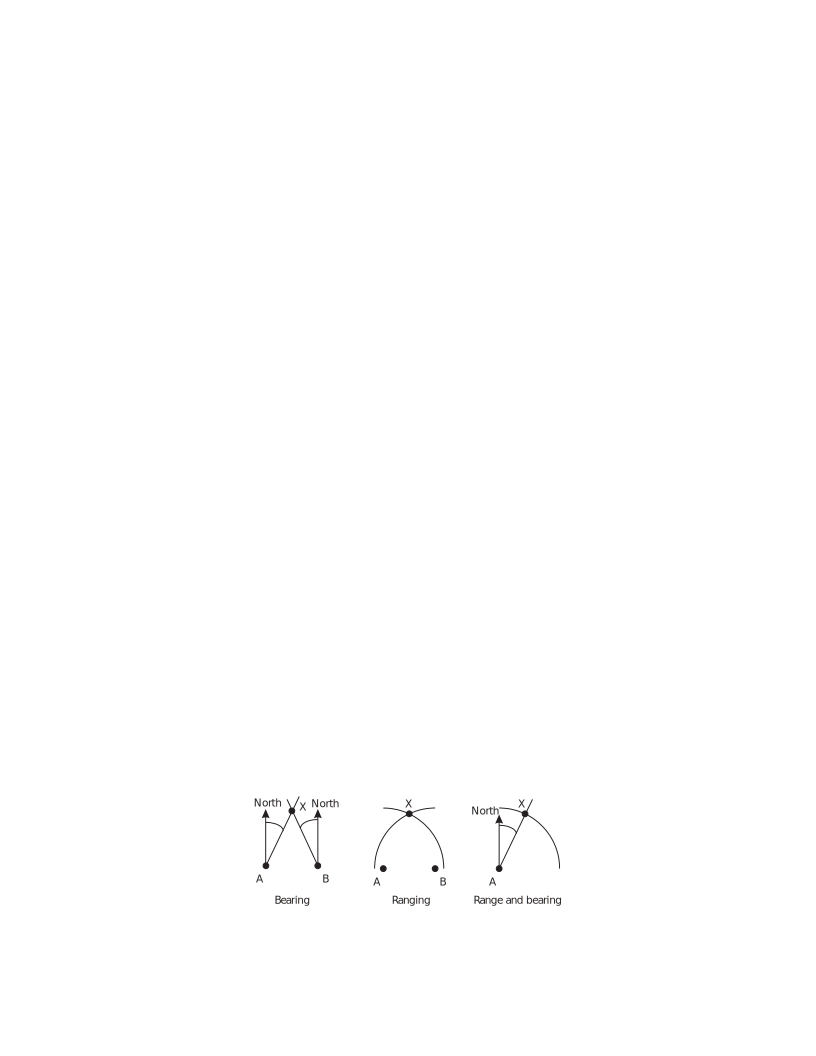
\includegraphics[width=\textwidth]{geometric_methods}    	
	\caption[Geometric positioning methods]{Geometric positioning methods: when the measurements obtained correspond to ranges, range differences or direction angles (bearing), in an ideal error free case, the position could be solved by the intersection of different combinations of the geometric elements defined by those these measurements. Source: Paul D. Groves \cite{groves_principles_2008}.}
	\label{fig:geometric}
\end{figure}
\begin{description}
	\item \textbf{Geometric Methods}
	
	The range, range difference and direction angles values provided by the previously described measurements are not individually enough to know the position of the moving node, as they represent circumferences, hyperboles or lines (spheres, hyperboloids and planes, in the three-dimensional case). 
	However, if several non-redundant measurements are available, a system of equations can be established and the unknown position solved.
	As can seen in the Figure~\ref{fig:geometric} for the two-dimensional case, there are different combinations of the geometrical constraints that can be combined to solve the unknown position: the intersection of three circumferences, of two lines, or a line and a circumference.
	In the three-dimensional case there are a greater number of combinations, being the most common one the intersection of four spheres.
	
	If only one type of geometric constraint is used, specific names are usually used: trilateration for ranges (circumferences or spheres intersections); multilateration for range differences (hyperbolas or hyperboloids intersections); and triangulation for angles (lines or planes intersections).
		
	% Unfortunately, the measurements are not error-free, which generates over-determined systems of equations. 
	% In addition, some of the $\boldsymbol{h}$ functions may be non-linear, so the systems can not commonly be solved analytically. 
	% If the $\boldsymbol{e}$ error is relatively small compared to the $\boldsymbol{z}$ measurements, approximate methods (e.g. least squares), linearized functions and iterative methods can be used.
	
	Unfortunately, since measurements are not usually error-free, the problem becomes an over-determined system of non-linear equations, which cannot commonly be solved analytically.
	If the $\boldsymbol{e}$ error is relatively small compared to the $\boldsymbol{z}$ measurements, iterative methods and approximate closed-form solutions (e.g. least squares) can be applied on linearized functions.
	%%%%%%%%%%%%%%%%%%%%%%%%%%%%%%%%%%%%%%%%%%%%%%%%%%%%%%%%%%%
	\item \textbf{Cost Function Minimization Methods}
	
	%Another approach for the cases where the analytical expression of function $\boldsymbol{h}$ is known and the error $\boldsymbol{e}$ is relatively small is to minimize a cost function such as the following one:
	For cases where the analytical expression of function $\boldsymbol{h}$ is known and the error $\boldsymbol{e}$ is relatively small, one approach is to minimize a cost function such as the following:
	\begin{equation}
	\label{eqn_costFunction}
		V(\boldsymbol{x})=\log p_e(\boldsymbol{z}-\boldsymbol{h}(\boldsymbol{x}))
	\end{equation}	
	where $p_e$ is the probability density function of the error $\boldsymbol{e}$. 	
	This optimization process will maximize the conditional probability $p(\boldsymbol{z}|\boldsymbol{x})$, so maximum likelihood estimators can be obtained for arbitrary error distributions.
	Additionally, it is possible to introduce protections against NLOS situations by converting the optimization problem into a constrained one.
	%%%%%%%%%%%%%%%%%%%%%%%%%%%%%%%%%%%%%%%%%%%%%%%%%%%%%%%%%%%
	\item \textbf{Fingerprinting Methods}
	
	When function $\boldsymbol{h}$ has no analytical expression, or it is difficult to obtain, or if the error $\boldsymbol{e}$ is significant compared to the measurements $\boldsymbol{z}$, methods from the machine learning field are commonly used, often known as fingerprinting.
	
	These methods are based on the previous generation of a map or database and convert the localization problem into a problem of inference or classification.
	Therefore, they consist of two phases: in the first one, known as offline calibration or training, values of the measurements of interest are collected in different positions of the area in which the localization service is to be provided.
	With these measurements, the database is constructed and, subsequently, during the online estimation phase, based on the specific measurements collected by the mobile node, the database is queried and the nearest or most probable position is returned as the estimated one.
	Techniques such as \emph{K-Nearest Neighbors} (KNN), Bayesian decision, \emph{Artificial Neural Networks} (ANN) or \emph{Support Vector Machines} (SVM) are usually applied for the estimation.
	
	These methods are based on relying solely on data collected during the offline phase.
	In this way, they do not need to know more features about the scenario, such as differentiating NLOS and LOS situations, knowing error distributions or even knowing the anchors' positions.
	This allows them to achieve good levels of accuracy.
	%However, their performance depends on the dimensionality of the measurements collected, the granularity with which the training data is done and the environment is not changed.
	However, performance depends on the dimensionality and granularity of the data collected during the offline phase and that the scenario is not modified.
	In addition, that offline calibration phase is often very time-consuming.
\end{description}	
%%%%%%%%%%%%%%%%%%%%%%%%%%%%%%%%%%%%%%%%%%%%%%%%%%%%%%%%%%%%%%%%%%%%%%%%%%%%%%%%%%%%%%%%%%%%
\subsection{Technologies}
\label{sec:2_2_3_technologies}		
The characteristics of signals that can be generated by the technology selected to implement a localization system will determine the type of measurements and estimation methods which are more appropriate, and what performance can be achieved in terms of accuracy, coverage and other requirements.
The following is a brief review of the main technologies used for position fixing based localization systems, focusing on the main strengths, weaknesses and areas of use of each of them.
\begin{description}
	\item \textbf{Global Navigation Satellite Systems}
		
	GNSS is the most widespread type of positioning system, mainly due to its almost global coverage and the availability of receivers integrated in a multitude of devices.
	
	The basis for their operation is the existence of a constellation of satellites whose orbits are known and it is therefore possible to know their position at any given time with good precision.
	The satellites emit electromagnetic signals in the microwave range, which contain modulated pseudo-random codes specifically designed to facilitate the estimation of the ToF between each satellite and receiver.
	Synchronization between the satellites is achieved by means of atomic clocks installed on them.
	On the other hand, the receiver's clock is of poorer quality and contains a certain synchronization error. However, since this error will be common to all satellites that are visible simultaneously, it can be eliminated if at least four satellites are received.
	By obtaining the ranges to at least four satellites, it is possible to compute the three-dimensional position of the receiver by trilateration.	

	The main weaknesses and disadvantages of these systems are:
	\begin{itemize}
		\item The power of the emitted signals is low, making it difficult to receive them with sufficient quality in, for instance, indoor environments or under trees.
		\item The troposphere and the ionosphere affect the propagation velocity of the electromagnetic wave, which results in an error in the estimation of the ranges and, hence, of the position.
		\item The existence of multipaths may also affect the estimation of ranges. This is especially common in NLOS scenarios, such as urban canyons.
		\item The relative geometry between the satellites and the receiver can generate different accuracies in different directions in space. This is usually known as \emph{Dilution of Position} (DoP).
		\item The necessary infrastructure, i.e. satellites, is expensive to produce, install and maintain.
	\end{itemize}	
	In the Table~\ref{table:ch2_GNSS_errors} it can be seen the orders of magnitude of the effect of the different error sources on the position error.
	However, depending on the complexity of the receiver and the amount of corrections applied, it is possible to achieve accuracies of the order of 10 meters for basic receivers to centimeter errors with more advanced solutions such as Differential GNSS or \emph{Real Time Kinematic} (RTK), although its use is mainly limited to outdoors scenarios.	
	\begin{table}[!t]
		%\renewcommand{\arraystretch}{1.3}
		\centering
		%\rowcolors{2}{gray!25}{white}
		\begin{tabular}{c c}
			\hline
			\rowcolor{gray!25}
			\bfseries Source of error & \bfseries Resulting position error\\
			\hline
			Satellites' clock and orbits& 0.5 m – 1 m\\
			\hline
			Atmospheric delays&1 m – 3 m\\
			\hline
			Multipath and NLOS signals&0.1 m – 100 m\\
			\hline
			Receiver thermal noise&0.1 m\\
		\end{tabular}
		\caption[Order of magnitude of the main GNSS position error sources]{Order of magnitude of the main position error sources in GNSS systems. Source:  SaPPART White paper \cite{noauthor_cost_2015}.}	
		\label{table:ch2_GNSS_errors}	
	\end{table}			
	%% Esta figura está bien pero es un poco pequeña %\InsertFig{GNSS.png}{fig:GNSS}{}{}{1}{}	
	%%%%%%%%%%
	\newpage
	\item \textbf{Wireless Local Area Networks}
	
	\emph{Wireless Local Area Networks} (WLAN) is a widely used set of wireless communication protocols (mainly IEEE 802.11) that can also be used for localization. 
	It is precisely this availability of already installed anchors in a multitude of environments and receivers in portable devices such as smartphones or laptops that is its main strength when it comes to being chosen as localization technology.
	%It operates in the ISM (Industrial, Scientific and Medical) bands and its coverage typically ranges 50-100 meters, surpassing other communication technologies.
	
	Propagation delay based measurements are often not used because of the poor results obtained. On the one hand, the off-the-shelf WLAN hardware is not usually ready to measure arrival times and, on the other hand, the usual bandwidth of WLAN systems (typically 20 MHz) implies that any multipath that occurs within 1-2 meters around the receiving node can be indistinguible from the direct path signal. This resolution is not enough for indoor environments with many obstacles in that range.
	
	RSS measurements are usually available on devices, but since WLAN anchors installation is usually designed to optimize communication, not positioning, and its coverage typically ranges 50-100 meters, NLOS situations are common. This makes it difficult to use an analytical propagation model, so fingerprinting-based techniques are the most common.
	
	With these techniques, accuracies between 1 and 10 meters are usually obtained, depending on the number of anchors and the density of calibration points.
	The main disadvantage of using WLAN fingerprinting is the high cost of performing the offline calibration phase, which can be degraded by changes in the environment.
	In addition, RSS values taken by different receiving devices may vary depending on the hardware and the power control strategies performed during data communications, which will also degrade the accuracy of the estimate.
	%%%%%%%%%%
	\item \textbf{Ultra Wideband}
	
	UWB is a communications technology that is defined as having an absolute bandwidth of at least 500 MHz or a relative bandwidth greater than 20\%. 
	It allows short-range communications (less than 100 meters), with high data rate and low power consumption but, thanks to its bandwidth, is especially useful for implementing localization systems based on propagation times. 
	Returning to the equation~\ref{eqn_heisenberg}, a bandwidth of 500 MHz implies a theoretical 5 centimeters range safe against multipaths.
	With these characteristics, position estimation with errors of a few tens of centimeters is achieved.
	However, as this is not a commonly used wireless technology, the systems currently developed are few and more expensive than other adopted technologies such as WLAN.
	
	%%%%%%%%%%
	\item \textbf{Sound}
	
	In contrast to electromagnetic waves, sound is a mechanical wave associated to a pressure oscillation transmitted through a medium, commonly the air.
	In general, signals in the ultrasound range are used, although there are also systems in the audible range to take advantage of the sound cards available in many devices.
	
	The characteristics of these signals involve a number of strengths and weaknesses that result in the use of only propagation delay measurements.
	Regarding their strengths:	
	\begin{itemize}
		\item Since the speed of sound propagation in the air is slow (around 343 m/s at 20°C), it is easy to detect and avoid multipaths, so centimeter-level accuracies can be achieved in indoor scenarios.
		\item This low propagation speed in comparison to the electromagnetic waves also facilitates the synchronization between nodes.
		\item Its hardware components are simple to implement and low cost.		
	\end{itemize}
	As for their weaknesses:
	\begin{itemize}
		\item Its main restriction is the low coverage mainly because of the high attenuation of these waves in the air.
		\item The velocity of sound propagation in the air is highly affected by temperature. This implies the implementation of compensation systems and avoiding environments with large temperature changes, such as outdoors.
		%\item In addition to NLOS and multipath situations, it is also sensitive to the Doppler effect if the nodes are moving at considerable speeds.		
		\item In addition to NLOS and multipath situations, due to the low propagation speed, these systems are also sensitive to the Doppler effect if the nodes are moving at considerable speeds.
	\end{itemize}
		
	%These characteristics mean that sounds are rarely used outdoors, often limited to confined spaces with few NLOS situations, and for applications requiring high levels of accuracy. 
	These characteristics make sound waves rarely be used outdoors, limiting their use to small spaces, avoiding NLOS situations and especially for applications that require great accuracy.
	In addition, the availability of high accuracy implies that the positions of the anchors must be known with at least the same accuracy, which complicates the installation process.
	%%%%%%%%%
	\item \textbf{Bluetooth Low Energy}	
	
	\emph{Bluetooth Low Energy} (BLE) is a wireless communication technology that offers simple devices the ability to exchange small amounts of data with very low power consumption.
	One of the most common operating modes is advertising, which allows a node to broadcast short messages periodically.
	These messages and their RSS measurements can be used to detect the proximity to one of these beacons and to estimate the position of a mobile node.
	
	The main advantages of this technology are the availability of receivers in many electronic devices, their high security, low cost and low consumption.
	The standard allows coverage ranges up to 100 meters but most beacons are usually visible from no more than 10 meters.
	
	This low coverage means that the main estimation technique is proximity and symbolic localization, which may be sufficient for some applications such as shopping centres or museums.
	However, it is also possible to apply fingerprinting techniques that give similar results to those achieved with WLAN and even to use analytical propagation models, which can achieve good results if the mobile node is about one meter away from the transmitter.
	
	In addition to the low coverage, another of its main disadvantages is that the low frequency of advertising can generate a latency in the estimation of the location, which makes real time applications difficult.	
\end{description}
% \InsertFig{tecnologies_comparison_Mautz.png}{fig:Mautz}{Comparison of accuracy and coverage offered by different technologies for position fixing localization method.}{Source: Rainer Mautz \cite{mautz_rainer_indoor_2012}}{1}{}
\begin{figure}[!t]
    \centering
	\includegraphics[width=\textwidth]{tecnologies_comparison_Mautz}    	
	\caption[Comparison of position accuracy and coverage offered by different technologies]{Comparison of accuracy and coverage offered by different technologies for position fixing localization method. Source: Rainer Mautz \cite{mautz_rainer_indoor_2012}.}
	\label{fig:Mautz}
\end{figure}

There are many other technologies that can be used to implement localization systems based on position fixing: cameras, infrared, RFID, visible light, magnetic fields, cellular networks and even television and FM radio signals. 
%The difference in the choice of technology is mainly reflected in the balance between accuracy and coverage, which is shown visually in the Figure~\ref{fig:Mautz}.
%When choosing a technology, one of the first features to consider is their balance between accuracy and coverage provided by the basic installation (obviously, it can always be scaled up to cover bigger areas).
When choosing a technology, one of the first features to consider is their balance between accuracy and coverage.
In Figure~\ref{fig:Mautz} can be seen a comparison of the most common technologies.
%In Figure~\ref{fig:Mautz} can be seen a comparison of this feature for the most common technologies, obviously considering only the installation of the basic infrastructure needed for each of them, since any solution can be scaled up to global coverage.
In addition to this compromise between accuracy and coverage, the main characteristic that summarizes the performance of the position fixing localization methods is that they offer better accuracy in the long-term than in the short-term. 
That is, there may be times when, because of NLOS or multipath situations, or temporary interferences, the position estimation error increases but, on average, it tends to be bounded.
\section{Dead Reckoning Localization Method}
\label{sec:2_3_DR}

The American Practical Navigator \cite{bowditch_originally_by_american_2017} defines DR as “a method for determining the estimated position of a vessel by advancing from a known fix of position along the vessel’s ordered course and speed”. 
In this way, maintaining a known course by using the compass and periodically measuring the forward speed, the boats were able to update their last known position frequently, without having to wait for the midday sun to calculate latitude and longitude with the sextant and chronometer.

Therefore, the fundamental characteristic of the DR method is that it is self-contained, that is, it does not require the existence of landmarks or reference points in the environment. 
It is only necessary to know the starting position and the heading and the speed during the integration period. 
In addition, DR also makes it possible to make future projections of the trajectory and, in this way, plan arrival times or avoid obstacles.

However, its main limitation is that, being a relative positioning method based on the last known position, if no corrective measurements are applied, errors accumulate unbounded over time, as depicted in Figure~\ref{fig:DR_error}.
Thus, although the origin of the term is not entirely clear, some theories indicate that ``Dead'' is due to the dangerousness
of such an accumulation of error. Other theories point to the possibility that it was a misspelling from the abbreviation of the term ``Deduced'' \cite{quinion_world_2007}.
% \InsertFig{deadreckoning_method.png}{fig:DR_error}{The Dead Reckoning Method}{The estimate of the position is obtained by updating an initial position using the course and distance traveled in that period. Being a relative method, there is an unbounded accumulation of errors. Source: Paul D. Groves \cite{groves_principles_2008}}{0.9}{}

\begin{figure}[!t]
    \centering
	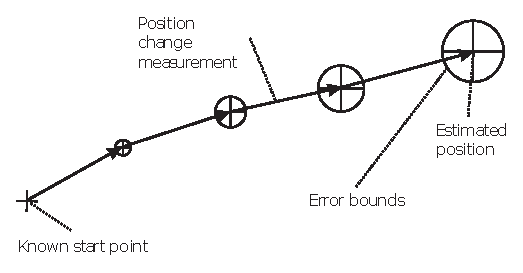
\includegraphics[width=0.8\textwidth]{deadreckoning_method}    	
	\caption[The Dead Reckoning method]{The DR method: the estimate of the position is obtained by updating an initial position using the course and distance traveled in that period. Being a relative method, there is an unbounded accumulation of errors. Source: Paul D. Groves \cite{groves_principles_2008}.}
	\label{fig:DR_error}
\end{figure}
The DR method is not only limited to maritime navigation and can be applied to any mobile element, such as aircraft, land vehicles or mobile robots. In fact, it is known that many mammals use similar path integration techniques to move around the environment.

Depending on the type of moving object, there exist different techniques and technologies for measuring the displacement, speed and course, so diverse as, for example, using a knotted rope for the measuring a boat’s speed  or an odometer for cars and bicycles. 
However, one of the most common technologies nowadays is the use of inertial sensors.
%%%%%%%%%%%%%%%%%%%%%%%%%%%%%%%%%%%%%%%%%%%%%%%%%%%
\subsection{Inertial Navigation Systems}
\label{sec:2_3_1_DR_INS}
Newton's first law of motion defines inertia as the property of bodies to maintain their state of motion, including both the magnitude and direction of their velocity, if no force is applied to them, or if the net force applied to them is null.
Likewise, an inertial reference system is one in which Newton's laws of motion are valid, that is, one that is not accelerated or rotating.

From these concepts arose the idea that, if it were possible to measure the forces acting on a body and trying to change its inertia, it would also be possible to calculate its changes in speed, course and position, regardless of the scenario and condition in which the movement occurs. 
This would be a major advance in the performance of DR-based navigation since, until then, the displacement, speed and course measurements required different techniques and instruments depending on whether the movement was by land, sea or air.

% In the late 19th century, the first inertial sensors capable of measuring angular velocity, known as gyroscopes, appeared. And since the early 20th century, the first accelerometers, capable of measuring linear accelerations.
In the mid-19th century, the first inertial sensors appeared: first, the gyroscopes, capable of measuring angular velocity and, around 70 years later, the accelerometers, capable of measuring linear accelerations.
However, it was not after the World War II, when inertial sensors of sufficient quality became available to construct navigation systems that would enable to track the position, speed and orientation of an object in space for a reasonable period of time and with acceptable accuracy. These systems are known as INS.

% \InsertFig{gimbal.pdf}{fig:gimbal}{Gimbaled INS or stable platform system}{Source: Oliver J. Woodman \cite{woodman_introduction_2007}}{0.5}{}
\begin{figure}[!t]
    \centering
	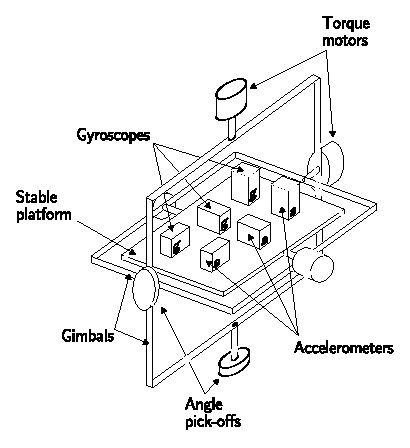
\includegraphics[width=0.6\textwidth]{gimbal}    	
	\caption[Gimbaled INS or stable platform system]{Gimbaled INS or stable platform system. Source: Oliver J. Woodman~\cite{woodman_introduction_2007}.}
	\label{fig:gimbal}
\end{figure}
The early INS used a configuration known as gimbaled INS or stable platform systems: the inertial sensors were mounted on a platform isolated from external rotations by motors that canceled the rotations detected by the gyroscopes, as shown in the Figure~\ref{fig:gimbal}. 
In this way, the accelerometer reference system was kept aligned with the navigation reference system.
%Subsequently, after correcting the value of the gravity on the accelerometers, the speed and position were obtained after successive integrations of the acceleration values.
After correcting the value of the gravity, the speed and position were obtained by successive integrations of the acceleration values.
%(figura~\ref{fig:gimbal_algorithm}).
This architecture was determined by the technological limitation of early gyroscopes and by the need to reduce the computational load that the transformation of accelerations from one reference system to another would imply.
%\InsertFig{gimbal_algorithm.pdf}{fig:gimbal_algorithm}{Gimbaled inertial navigation algorithm}{Source: \cite{woodman_introduction_2007}}{1}{}
Subsequently, with the improved performance of gyroscopes and the availability of increased computing power, a configuration in which inertial sensors were rigidly mounted on the moving object was used. 
This configuration is known as strapdown and, in exchange for greater computational complexity, smaller and mechanically simpler INS are achieved.
Currently, strapdown INS is the most widely used configuration. 

Next, a general description of the implementation of the strapdown INS is presented, introducing the basic types of inertial sensors, an overview of the algorithm formulation and some cumulative error reduction techniques that can be applied so that the system remains self-contained.
There are many references in the literature to these and other aspects of the INS, such as \cite{grewal_global_2001, titterton_strapdown_2004, woodman_introduction_2007, groves_principles_2008, groves_navigation_2015}.
\subsubsection{Inertial Sensors}
\label{sec:2_3_1_1_DR_INS_IMU}
\begin{description}
	\item \textbf{Accelerometers}
	% \InsertFig{accelerometer.pdf}{fig:accelerometer}{Simple mechanical accelerometer}{Source: Paul D. Groves \cite{groves_navigation_2015}}{0.8}{}
	\begin{figure}[!t]
		\centering
		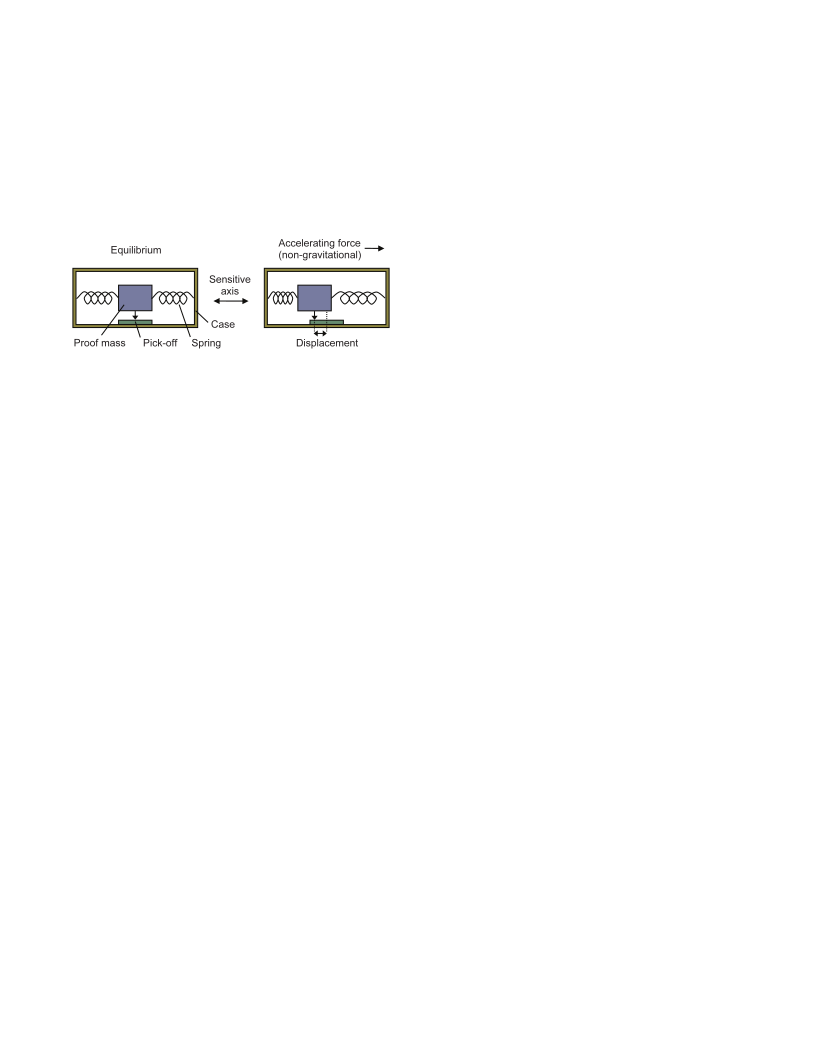
\includegraphics[width=0.8\textwidth]{accelerometer}    	
		\caption[Simple mechanical accelerometer]{Simple mechanical accelerometer. Source: Paul D. Groves \cite{groves_navigation_2015}.}
		\label{fig:accelerometer}
	\end{figure}
	
	In the Figure~\ref{fig:accelerometer} can be seen the structure of a basic mechanical accelerometer.
	The basis of its operation is that the relative position between the test mass of the interior and the case is proportional to the force applied in the direction of the measuring axis. 
	That is, when an acceleration is applied to this axis, the case moves in relation to the test mass through the springs that connect them.
	%Accelerometers only measure non-gravitational accelerations, known as ``specific force'', since accelerations due to gravity affect the entire accelerometer set equally and are not distinguishable.
	%Therefore, if the accelerometer is in free fall, the specific force and, therefore, also the output of the accelerometer will be zero. 	
	Accelerometers only measure non-gravitational accelerations, known as ``specific force''.
	This is because gravity affects the entire sensor and is therefore not distinguishable.
	%This implies that, if the accelerometer is in free fall, the specific force will be zero and therefore the measurement provided by the sensor will also be zero.
	This implies that, if the accelerometer is in free fall, the specific force will be zero and so will be the measurement provided by the sensor.
	On the other hand, if the accelerometer is static and its sensitive axis is parallel to the direction of gravity, the output value of the sensor will be the magnitude of gravity.
	That is why, when integrating accelerations in an INS, it is necessary to know the local value of gravity in order to correct the measurements offered by the accelerometers.	
	Current accelerometers are based on more advanced designs such as pendulums or vibrating beams, built both mechanically and in solid state \cite{titterton_strapdown_2004}.
	
	%%%%%%%%%%%
	%\newpage
	\item \textbf{Gyroscopes}
	
		% \begin{figure}[!t]
			% \centering
			% \subfloat[\textbf{Effect on a ring based gyroscope.}]{
				% 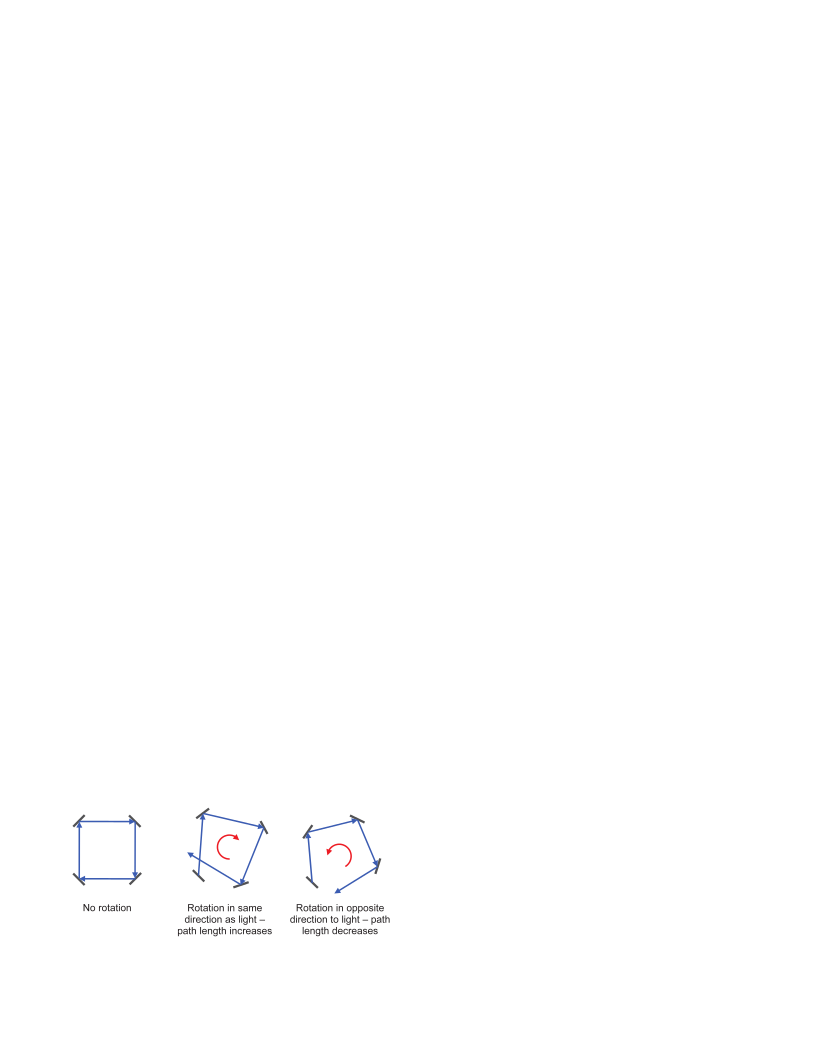
\includegraphics[scale=1.2]{gyro_fiber.pdf}
				% \label{fig:gyro_fiber}}
			% \vfil
			% \subfloat[\textbf{Gyroscope based on a vibrating structure.}]{
				% 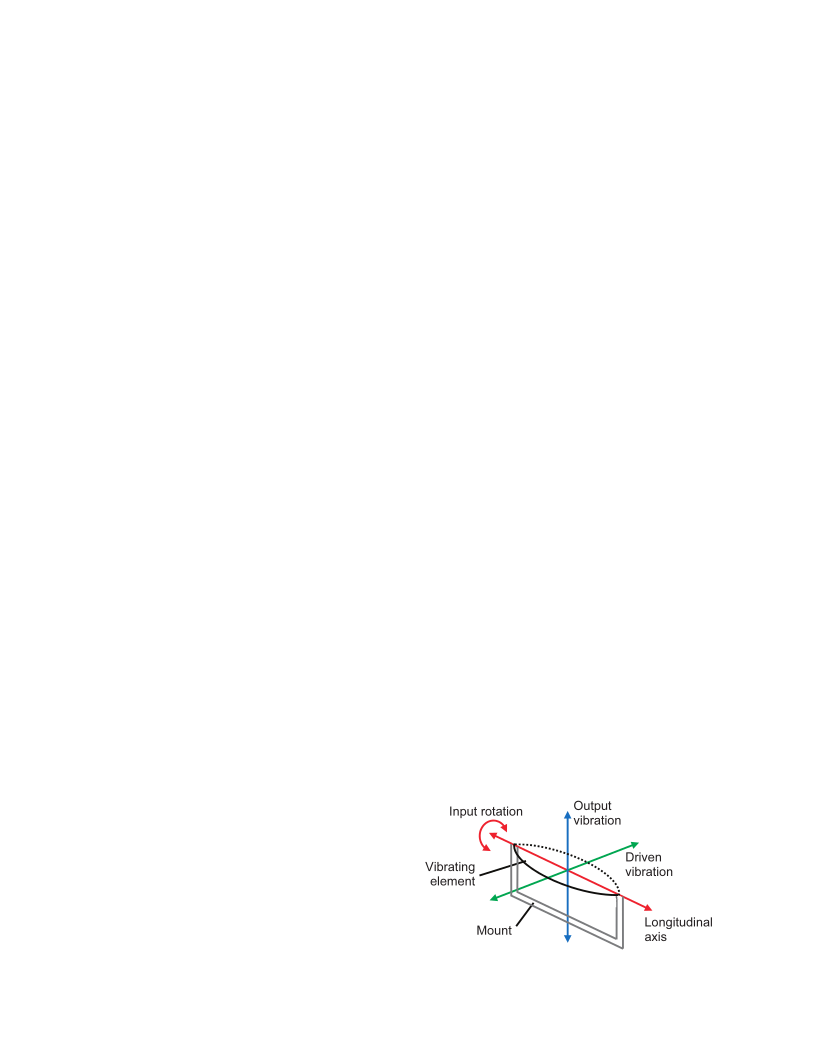
\includegraphics[scale=1]{gyro_vibrating.pdf}
				% \label{fig:gyro_vibrating}}
			% \caption[Working principle of different types of gyroscopes]{Working principle of different types of gyroscopes. Source: Paul D. Groves \cite{groves_navigation_2015}.}
			% \label{fig:MEMS_gyro_types}
		% \end{figure}	
	The first mechanical gyroscopes were based on a spinning wheel mounted on a gimbaled structure, similar to the one shown in Figure~\ref{fig:gimbal}, which allows it to rotate in all three axes.
	Due to the conservation of the angular momentum, the spinning wheel resists to change its orientation and, by reading the pick-offs, the orientation angles can be known.
	%\InsertFig{gyroscope.pdf}{fig:gyroscope}{A conventional mechanical gyroscope}{Source: \cite{woodman_introduction_2007}}{0.5}{}
	
	In contrast, modern gyroscopes offer angular rates instead of orientation angles. 
	They are usually built as fiber optic rings or vibrating structures.
	The former are based on a beam of light emitted through a ring of known length. By measuring the time it takes to go through it, it is possible to know how much the ring turned and in what direction.
	%if the ring has turned, how much it has turned, and in what direction.
	The latter use vibrating elements to measure the Coriolis acceleration and, from it, the angular velocity.
	Diagrams of both types of gyroscopes can be seen in Figure~\ref{fig:MEMS_gyro_types}.	
	%\InsertFig{gyro_fiber.pdf}{fig:gyro_fiber}{Effect on a ring based gyroscope}{Source: \cite{groves_navigation_2015}}{0.8}{}
	%\InsertFig{gyro_vibrating.pdf}{fig:gyro_vibrating}{Gyroscope based on a vibrating structure}{Source: \cite{groves_navigation_2015}}{0.8}{}			
		\begin{figure}[!t]
			\centering
			\subfloat[\textbf{Effect on a ring based gyroscope.}]{
				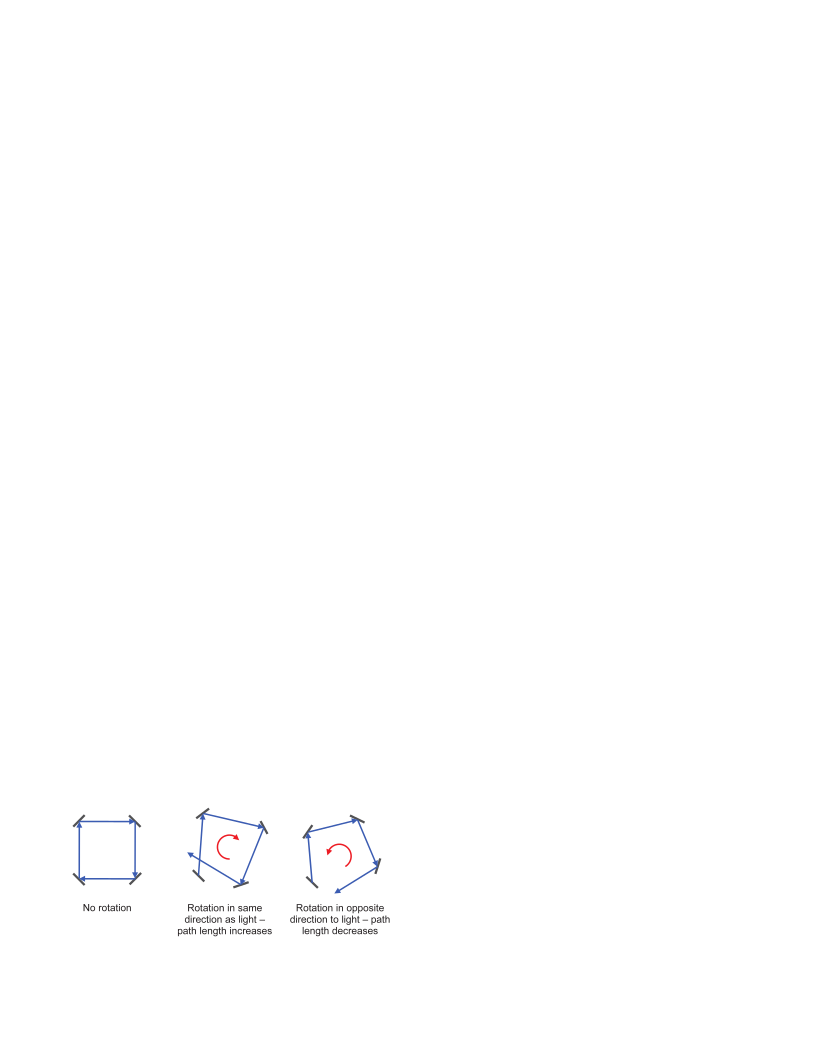
\includegraphics[scale=1.2]{gyro_fiber.pdf}
				\label{fig:gyro_fiber}}
			\vfil
			\subfloat[\textbf{Gyroscope based on a vibrating structure.}]{
				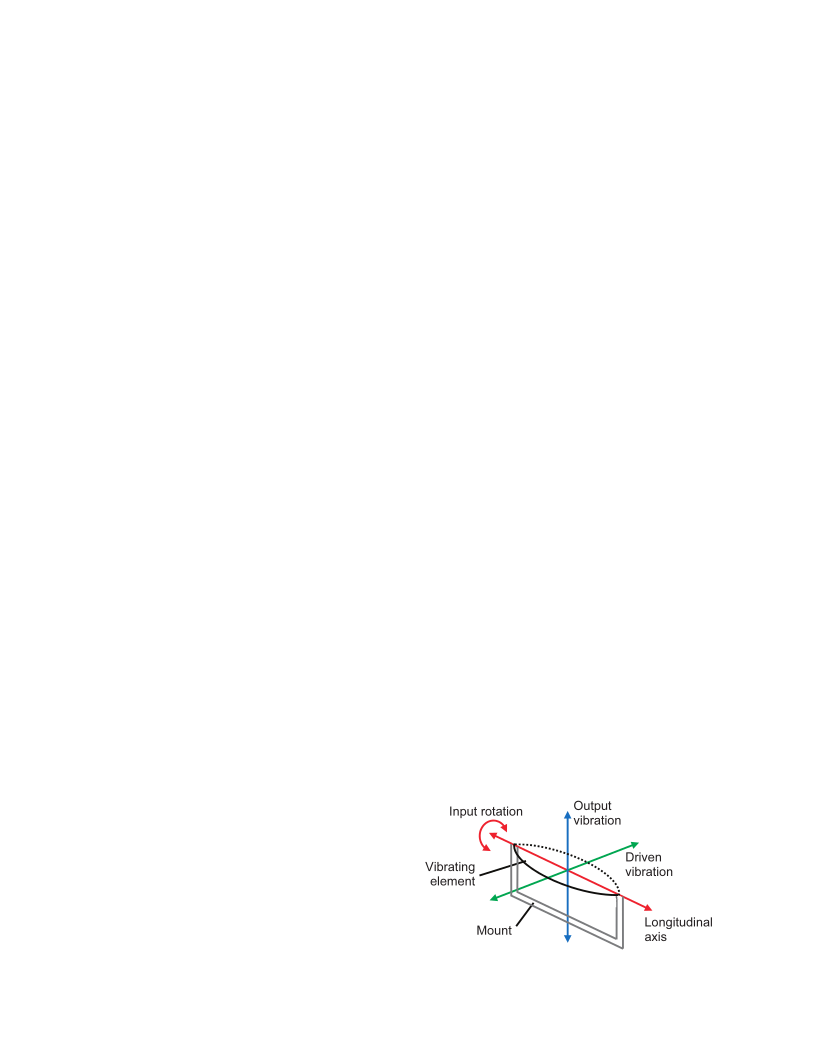
\includegraphics[scale=1]{gyro_vibrating.pdf}
				\label{fig:gyro_vibrating}}
			\caption[Working principle of different types of gyroscopes]{Working principle of different types of gyroscopes. Source: Paul D. Groves \cite{groves_navigation_2015}.}
			\label{fig:MEMS_gyro_types}
		\end{figure}	
	%%%%%%%%%%%
	\item \textbf{Inertial Measurement Units}
	
	A body that can move without restrictions in a three-dimensional space has six degrees of freedom: translations along three perpendicular axes (forward/backward, up/down, left/right) and changes in orientation through rotation about three perpendicular axes.
	Therefore, at least three accelerometers and three gyroscopes will be required to implement an INS in such a scenario.
	
	Accordingly, it is common to group several inertial sensors into a single device, known as \emph{Inertial Measurement Unit} (IMU), which generally contains those three accelerometers and three gyroscopes placed in orthogonal directions.
	In addition, IMUs may contain additional sensors, such as magnetometers and barometers, and signal matching and calibration capabilities, power supply and communication interfaces.	
	%%%%%%%%%%%%
	\item \textbf{Inertial Sensors' Errors}
	
	Inertial sensors are not perfect devices and have different types of errors. These are some of the most important:
	\begin{itemize}
		\item Bias: It is the offset between the measurement and the actual value. It is usually the biggest source of error.
		\item Scale-factor: This is the separation between the ratio of actual to estimated values and the unit slope line. That is, it indicates whether the error is proportional to the value of the measured variable. 
		\item Cross-coupling: This occurs when the physical quantities produced in one axis are ``felt'' on other perpendicular axes of the sensor. This is usually due to misalignment during sensor construction.
		\item Random errors: They are due to mechanical and electrical sources. Usually known as ``random walk'' because of the effect of its integration.
	\end{itemize}	
	
	The first three types of errors are systematic and are made up of four fundamental components:
	\begin{itemize}
		\item Fixed contribution: Present each time the sensor is used.
		\item Effect of temperature: Temperature changes affect sensor response.
		\item Run-to-run variation: It is the variation of each error source between different uses of the sensor.
		\item In-run variation: It is the variation of each error source during one use of the sensor.
	\end{itemize}
	The first two error components can be eliminated or reduced through calibration processes. 
	Not the latter two, which can only be corrected by the use of external information.	
	This way, an error model of the IMU's accelerometers can be written:
	\begin{equation}
	\label{eqn_acc_error}
		\boldsymbol{\hat{f}}=\boldsymbol{b_a}+(\boldsymbol{I_3}+\boldsymbol{M_a})\boldsymbol{f}+\boldsymbol{w_a}
	\end{equation}	
	where $\boldsymbol{\hat{f}}$ is the specific force vector measured by the IMU's accelerometers, $\boldsymbol{b_a}$ the accelerometers' bias vector, $\boldsymbol{I_3}$ is the identity matrix, $\boldsymbol{M_a}$ is the matrix of the coefficients of the accelerometers scale-factor (diagonal elements) and cross-coupling errors (off-diagonal elements), $\boldsymbol{f}$ is the true specific force vector and $\boldsymbol{w_a}$ is the random-noise vector.
	And similarly for gyroscopes:
	\begin{equation}
	\label{eqn_gyr_error}
		\boldsymbol{\hat{\omega}}=\boldsymbol{b_g}+(\boldsymbol{I_3}+\boldsymbol{M_g})\boldsymbol{\omega}+\boldsymbol{G_g}\boldsymbol{f}+\boldsymbol{w_g}
	\end{equation}		
	where $\boldsymbol{\omega}$ is referred to the angular rate, $\boldsymbol{G_g}$ is the matrix of errors dependent on the accelerations suffered by the gyroscopes, and the rest of symbols are analogous to the accelerometer case.
	%%%%%%%%%%%%
	\item \textbf{MEMS Technology}	
	
	Among the different types of gyroscopes and accelerometers available, the best performances are usually associated with those of greater size and mechanical complexity.
	This has consequences in terms of usability, as it impacts on their portability and cost, for example.
		
	Since the end of the 20th century, the development of the MEMS technology has made it possible to develop small, lightweight, low-cost inertial sensors. 
	This has allowed them to be included in a multitude of portable devices, such as smartphones or wearable devices, and, therefore, to be available for pedestrian applications.
	However, although its performance continues to improve, this reduction in size leads to higher levels of error, as shown in Figure~\ref{fig:MEMS_performance}.	
	It is therefore common for inertial sensors to be classified according to their accuracy in categories such as marine, aviation, tactical or consumer.			
	\begin{figure}[!t]
		\centering
		\subfloat[\textbf{Accelerometers}]{
			\includegraphics[]{MEMS_acc}
			\label{fig:MEMS_acc}}
		\vfil
		% \subfloat[\textbf{Accelerometers}]{
			% \includegraphics[width=0.8\textwidth]{MEMS_acc_old.png}
			% \label{fig:MEMS_acc}}
		% \vfil		
		\subfloat[\textbf{Gyroscopes}]{
			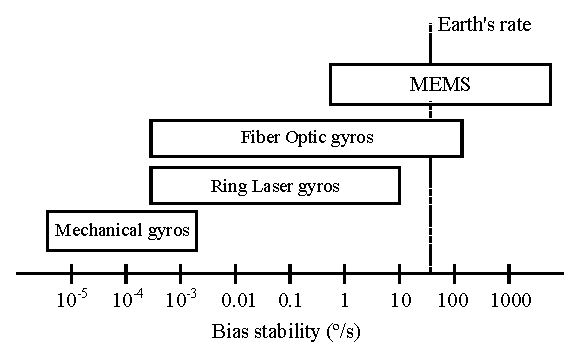
\includegraphics[]{MEMS_gyro}
			\label{fig:MEMS_gyro}}
		% \subfloat[\textbf{Gyroscopes}]{
			% 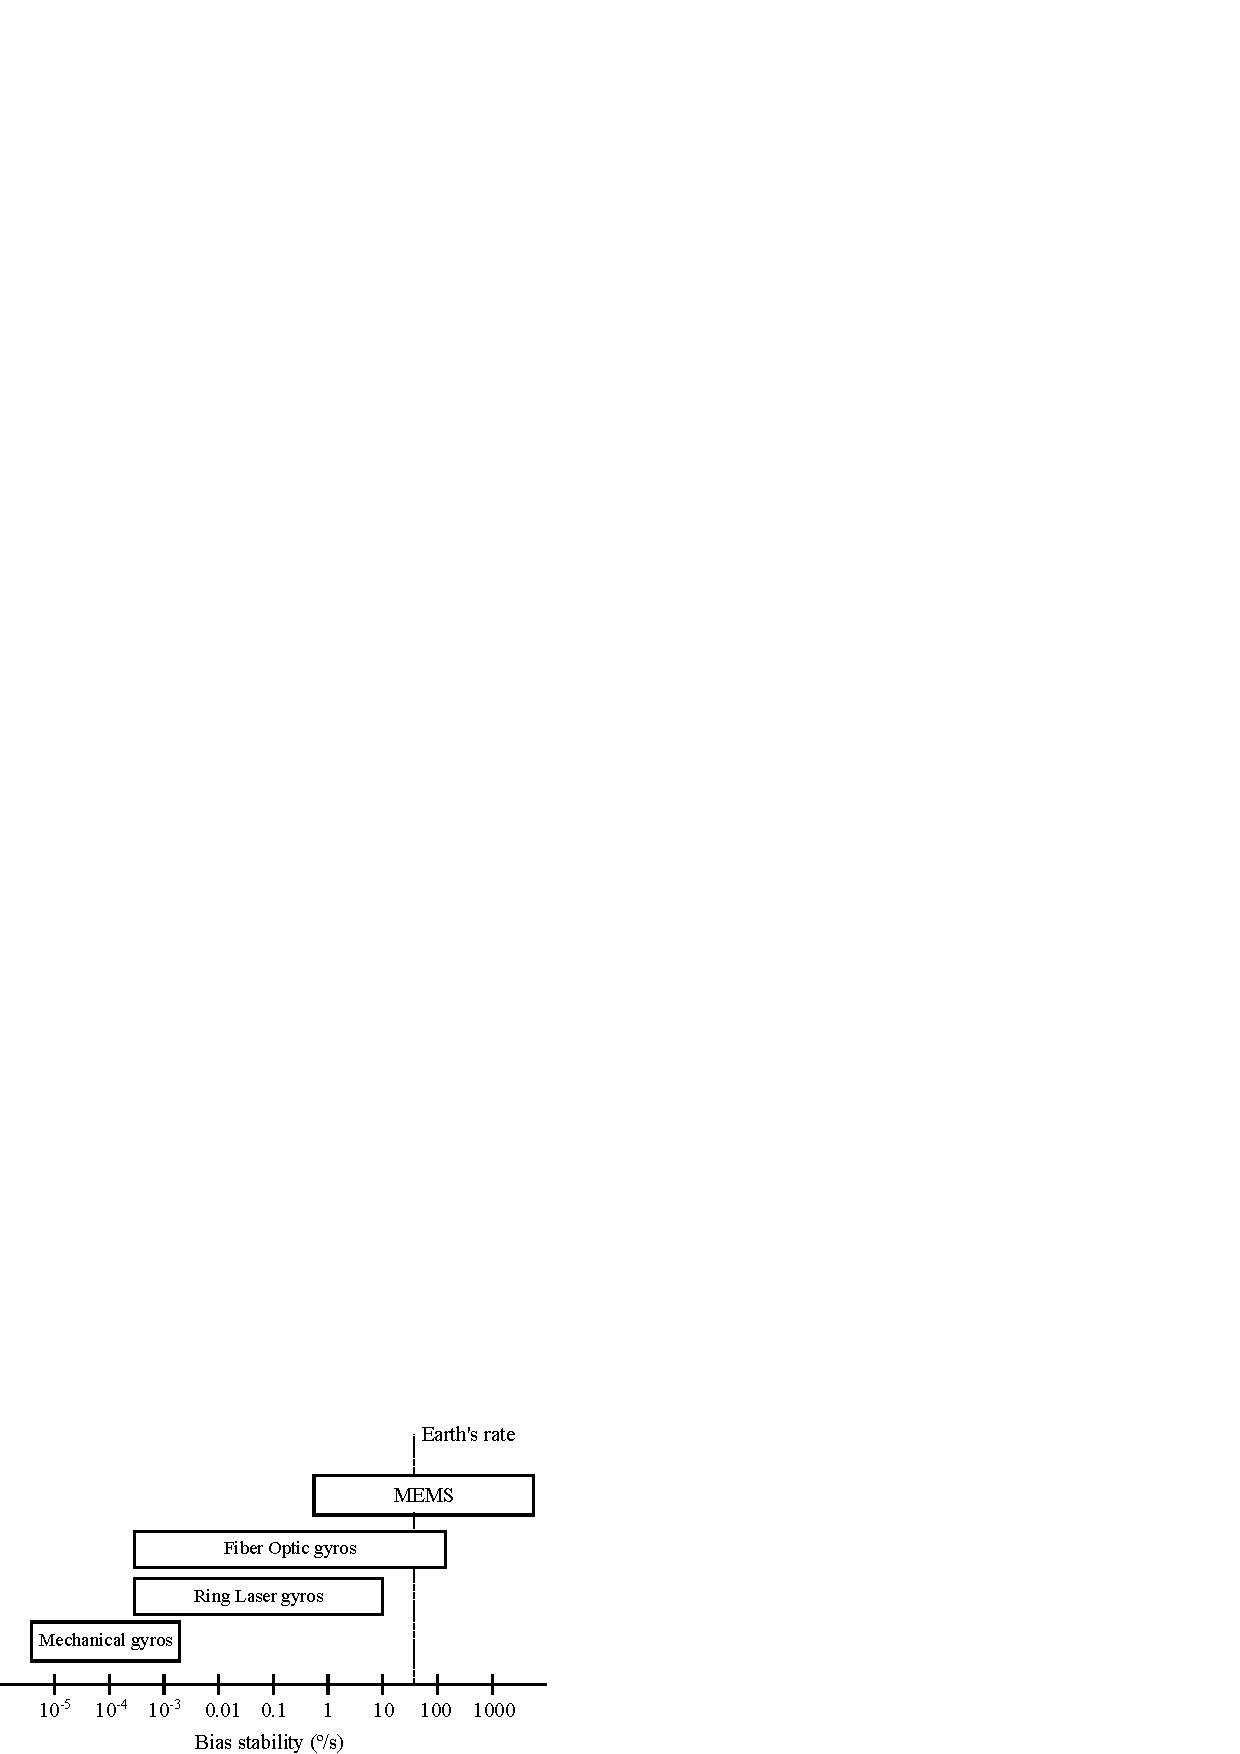
\includegraphics[width=0.8\textwidth]{MEMS_gyro.png}
			% \label{fig:MEMS_gyro}}			
	    \caption[Performance comparison of different types of inertial sensors]{Performance comparison of different types of inertial sensors. Source: D.H. Titterton and Weston\cite{titterton_strapdown_2004}.}
		\label{fig:MEMS_performance}
	\end{figure}	
\end{description}

\subsubsection{Strapdown INS Mechanization}
\label{sec:2_3_1_2_DR_INS_SINS}
The following will briefly explain the fundamental steps of the strapdown INS algorithm. 
There are different variants of this method, known as mechanizations, depending on which system is chosen as reference frame.
In this case it will be considered that navigation is required with respect to a fixed reference frame. That is, an inertial reference system, which is neither rotating nor accelerated.

A fixed reference system in relation to the Earth is not inertial, as the planet rotates and moves through the universe.
Since accelerometers and gyroscopes provide measurements with respect to an inertial system, the rotations and the accelerations associated with the Earth's movement (centripetal, Coriolis and Euler) should be taken into account when navigating with respect to the it.
However, if we limit ourselves to the case of pedestrians and MEMS-based IMUs, the low speed at which we walk and the noise levels of the sensors (as can be seen in the Figure~\ref{fig:MEMS_gyro}) allow to assume that the Earth is a fixed reference frame.

Throughout this section, the subscripts b (body frame) and g (global frame) are used to indicate the frame of reference in which vector quantities are measured, as can be seen in the Figure~\ref{fig:body_reference}.
% \InsertFig{body_reference.pdf}{fig:body_reference}{The body and global frames of reference}{Source: Oliver J. Woodman \cite{woodman_introduction_2007}}{0.5}{}
\begin{figure}[!t]
    \centering
	
\includegraphics[width=0.5\textwidth]{body_reference}    	
	\caption[The body and global frames of reference]{The body and global frames of reference. Source: Oliver J. Woodman~\cite{woodman_introduction_2007}.}
	\label{fig:body_reference}
\end{figure}

The strapdown INS mechanization can be divided into 4 basic steps: orientation update, accelerations projection, gravity correction and integration.

Knowing the orientation of the moving object with respect to the global frame is necessary for several reasons.
On the one hand, because it is essential for later projecting the accelerations from the body frame to the global frame before integrating them;
And, on the other hand, because, in general, orientation cannot be assumed from the direction of traveling. 
Think, for example, of a person walking sideways: the direction in which he looks does not coincide with that of his displacement.

There are different ways to represent orientations.
Some of the most common ones are rotation matrices, Euler angles and quaternions \cite{shuster_survey_1993}. 
In this case, we will use rotation matrices.	
It can be shown that, using the small angle approximation, the variation over time of a rotation matrix can be expressed by the following differential equation (\cite{titterton_strapdown_2004, woodman_introduction_2007}):
\begin{equation}
\label{eqn_dcm_ed}
	\boldsymbol{\dot{C}}(t)=\boldsymbol{C}(t)\boldsymbol{\Omega}(t)
\end{equation}	
which has the solution:
\begin{equation}
\label{eqn_dcm_ed_sol}
	\boldsymbol{C}(t)=\boldsymbol{C}(0)\cdot exp \left( \int_{0}^{t}\boldsymbol{\Omega}(t) dt \right)
\end{equation}		
where
\begin{equation}
\label{eqn_skew_matrix}
	\boldsymbol{\Omega}(t)=
	\begin{pmatrix}
		0&-\omega_{bz}(t)&\omega_{by}(t)\\
		\omega_{bz}(t)&0&-\omega_{bx}(t)\\
		-\omega_{by}(t)&\omega_{bx}(t)&0
	\end{pmatrix}		
\end{equation}	
is the skew symmetric form of the angular rate vector $\omega_b(t)$.

Since most gyroscopes are digital and they provide angular rate values periodically ($\triangle t$), it can be shown that the orientation update equation after each successive gyroscope sample has the following form:
\begin{equation}
\label{eqn_dcm_update}
	\boldsymbol{C}(t+\triangle t)=\boldsymbol{C}(t) \left( \boldsymbol{I}+\frac{\sin \sigma}{\sigma}\boldsymbol{B}+\frac{1-\cos\sigma}{\sigma^2}\boldsymbol{B}^2 \right)
\end{equation}
where $\sigma=|\omega_b\triangle t|$ and the matrix $\boldsymbol{B}$:
\begin{equation}
\label{eqn_skew_matrix_upd}
	\boldsymbol{B}=
	\begin{pmatrix}
		0&-\omega_{bz}\triangle t&\omega_{by}\triangle t\\
		\omega_{bz}\triangle t&0&-\omega_{bx}\triangle t\\
		-\omega_{by}\triangle t&\omega_{bx}\triangle t&0
	\end{pmatrix}		
\end{equation}	

These expressions assume infinitesimal rotations and sampling periods. Therefore, the sampling frequency of gyroscopes should, in general, be as high as possible, so that the angular velocity can be considered as constant between each measurement period.

Once the current orientation of the object is obtained, it is possible to project the accelerations from the IMU's body frame to the global frame:
\begin{equation}
\label{eqn_acc_proy}
	\boldsymbol{a}_g(t)=\boldsymbol{C}(t)\boldsymbol{a}_b(t)
\end{equation}
where $\boldsymbol{a}_b(t)=(a_{bx}(t),a_{by}(t),a_{bz}(t))^T$ are the measurements from the accelerometers.

Finally, the only thing left to do is to correct the gravity, expressed in global frame ($\boldsymbol{g}_g$), and carry out the successive integrations.
In a similar way to gyroscopes, the accelerometers deliver their measurements periodically, so integrating by the rectangular rule, the update equations will be:
\begin{equation}
\label{eqn_acc_int}
	\boldsymbol{v}_g(t+\triangle t)=\boldsymbol{v}_g(t)+\triangle t \cdot (\boldsymbol{a}_g(t+\triangle t)-\boldsymbol{g}_g)
\end{equation}
\begin{equation}
\label{eqn_vel_int}
	\boldsymbol{s}_g(t+\triangle t)=\boldsymbol{s}_g(t)+\triangle t \cdot (\boldsymbol{v}_g(t+\triangle t))
\end{equation}
where $\boldsymbol{v}_g(t)$ y $\boldsymbol{s}_g(t)$ are the velocity and position of the moving body, expressed in the global frame, at time $t$.
A general diagram of the algorithm just explained can be seen in the Figure~\ref{fig:strapdown_algorithm}.
% \InsertFig{strapdown_algorithm.pdf}{fig:strapdown_algorithm}{Strapdown INS mechanization for a fixed reference frame}{Source: Oliver J. Woodman \cite{woodman_introduction_2007}}{1}{}
\begin{figure}[!t]
    \centering
	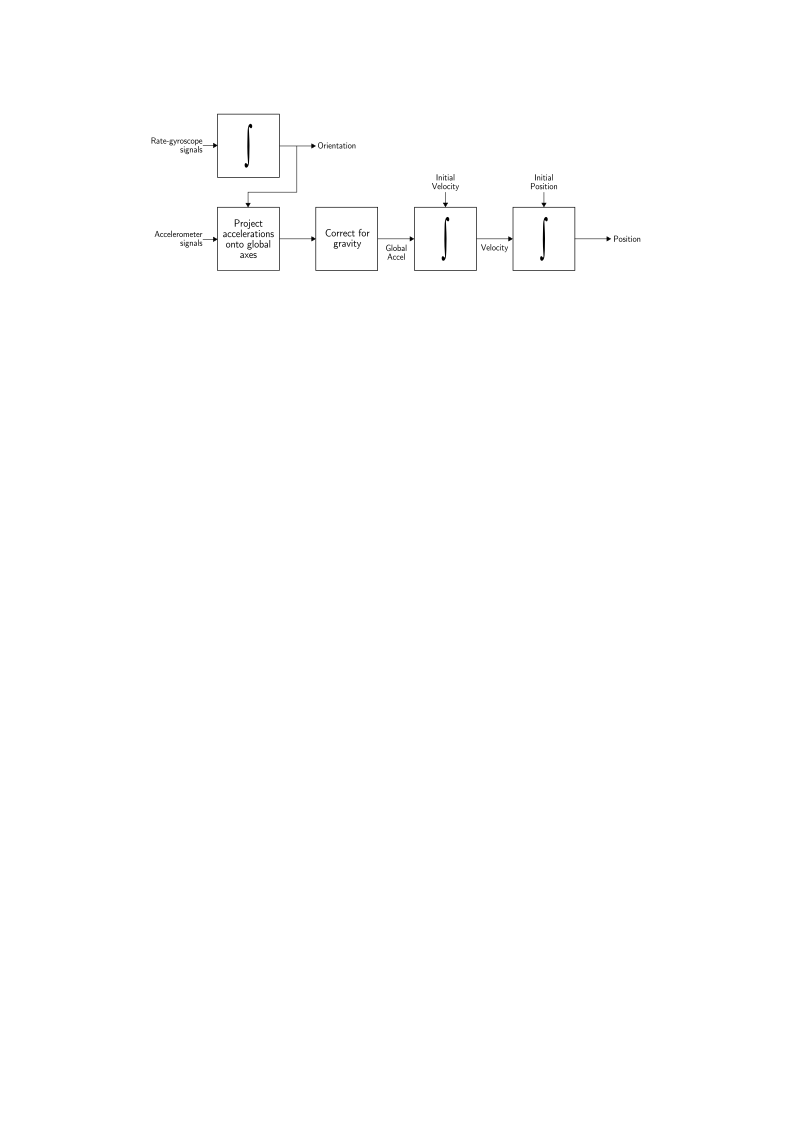
\includegraphics[width=1\textwidth]{strapdown_algorithm}    	
	\caption[Strapdown INS mechanization for a fixed reference frame]{Strapdown INS mechanization for a fixed reference frame. Source: Oliver J. Woodman~\cite{woodman_introduction_2007}.}
	\label{fig:strapdown_algorithm}
\end{figure}
\subsubsection{Drift Reduction Techniques}
\label{sec:2_3_1_3_DR_INS_ZUPT}
As discussed in Section~\ref{sec:2_3_1_1_DR_INS_IMU}, inertial sensors contain errors and, since strapdown INS is an integration-based method, those errors will also be integrated and will accumulate unbounded over time.
On the one hand, the errors of the gyroscopes will propagate as orientation errors when integrated, which will grow proportionally with time.
On the other hand, the errors of the accelerometers will propagate linearly in time as velocity errors and, after the second integration, as position errors in a quadratic rate.
However, the orientation error also propagates as position error since it causes that the projection of the accelerations is done wrongly and, therefore, the correction of gravity as well.
Therefore, the total position error grows cubically in time.
%In fact, for many applications that orientation error is critical, since the magnitude of the gravity can be much greater than the average accelerations that the object undergoes, reason why any small error of orientation will have a great impact in the position error .
%In fact, for many applications, this orientation error is critical: When the magnitude of the gravity can be much greater than the average accelerations that the object undergoes, any small orientation error will have a great impact in the position error .
%De hecho, debido a la magnitud de la gravedad, cualquier pequeño error de orientación puede generar un error de posición mayor que el debido a los errores de los acelerómetros.
In fact, orientation error is critical: due to the magnitude of the gravity on Earth, any small orientation error will have a great impact in the position error.

The position error accumulation is especially evident if inertial sensors based on MEMS technology are used.
In the Figure~\ref{fig:MEMS_error_position} the position error accumulation rate for a static strapdown INS using a medium-low cost IMU is shown.
As can be seen, this position error rate makes navigation unfeasible after a few seconds.
Therefore, the use of INS systems based on MEMS IMUs, which are the most convenient for pedestrians, seems complicated.
And, in general, although high precision inertial sensors are used, the use of INS is limited in time.
% \InsertFig{MEMS_error_position.pdf}{fig:MEMS_error_position}{Average drift position when applying strapdown INS to a static MEMS-based IMU's measurements}{Source: Oliver J. Woodman \cite{woodman_introduction_2007}}{1}{}
\begin{figure}[!t]
    \centering
	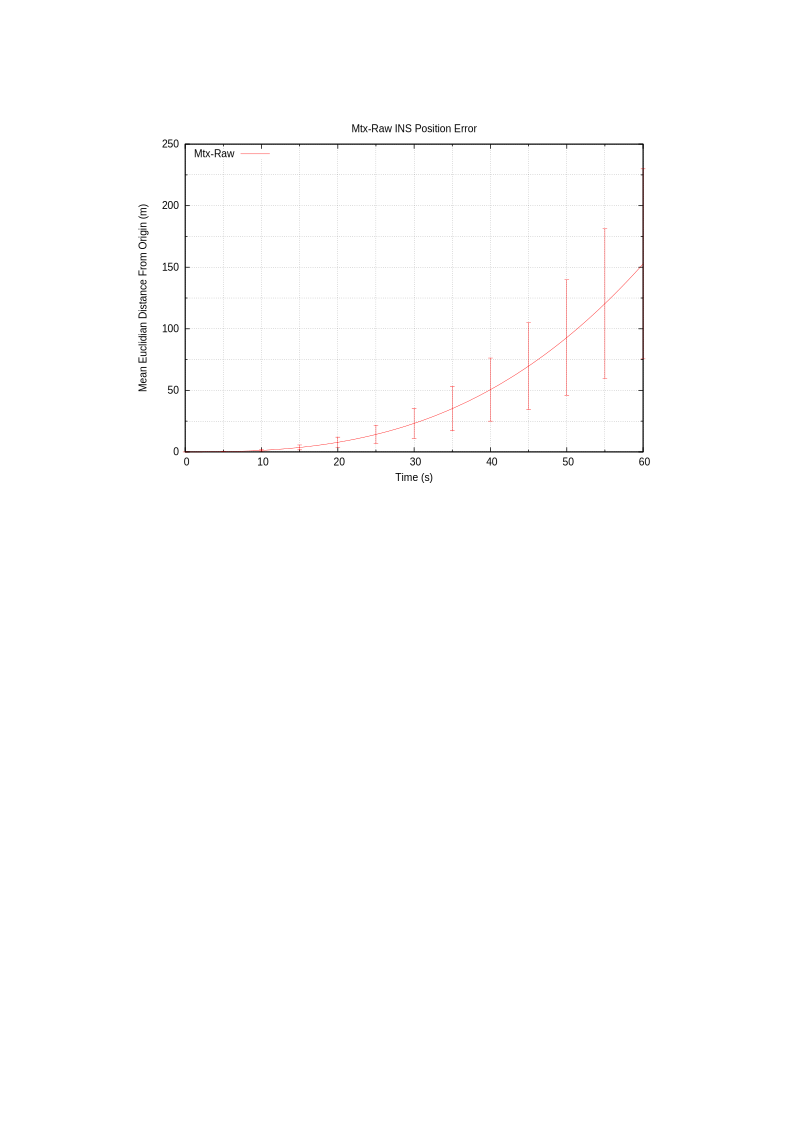
\includegraphics[width=1\textwidth]{MEMS_error_position}    	
	\caption[Average drift position of a static strapdown INS with a MEMS-based IMU]{Average drift position of a static strapdown INS with a MEMS-based IMU. Source: Oliver J. Woodman~\cite{woodman_introduction_2007}.}
	\label{fig:MEMS_error_position}
\end{figure}
However, as will be seen in the following Section~\ref{sec:2_4_fusion}, by merging with other technologies and additional information sources, it is possible to use INS systems in such a way that they are useful for navigation.
%Among the different types of information that can be merged, in this section we will highlight those that allow the system to remain self-contained:
Among the different types of information that can be merged, those that allow the system to remain self-contained are now introduced.
\begin{description}
	\item \textbf{A priori knowledge about object's dynamic}
	
	The knowledge about the characteristics of the movement of an object can give the possibility of identifying scenarios in which the value of some of the variables describing its movement is known a priori and, therefore, some corrections can be applied under that assumption.

	One of the most common corrections are the ZUPT, which consist in detecting the moments in which it is known that the object is still. This allows to correct the value of the estimated velocity at that moment. In this way, the rate of accumulation of the velocity and position error is reduced, providing a longer operation time the INS.

	Another corrective measure is the one known as \emph{Zero-Angular Rate Updates} (ZARU), which, likewise, consists of detecting the static moments of the object but, in this case, to estimate the value of the gyroscopes' bias, since it can be assumed that their output values should be zero at those moments. In this way, the growth rate of the orientation error is reduced, which also impacts the estimation of the velocity and position.
	
	These techniques have been successfully applied to different scenarios, such as underwater navigation \cite{huddle_trends_1998}, oil drilling \cite{ledroz_fog-based_2005} or geographic mapping \cite{grejner-brzezinska_bridging_2001}, and, thanks to the characteristics of the human gait, it can also be applied to pedestrians.
	Through the use of foot-mounted IMUs, it is possible to detect the moments when the foot is still on the ground, which occurs periodically at each footstep.
	In this way, it is possible to periodically correct INS errors and reduce the accumulation of the position error to a rate proportional to the number of strides.
	Furthermore, the detection of the stance periods is possible using only the acceleration and angular rate signals, so the system remains self-contained.
	With this solution, position errors close to 1\% of the traveled distance can be achieved using MEMS IMUs, surpassing even ``pure'' INS systems with higher performance IMUs.
	The work of Eric Foxlin is recognized for being the first to use efficiently the ZUPT technique for foot-mounted IMUs \cite{foxlin_pedestrian_2005}, and a good explanation can also be found in the work of Jiménez \emph{et al.} \cite{jimenez_indoor_2010}.	
	%%%%%%%%%%%%%%%%%%%%%%%%%%%%%%%%%%%
	\item \textbf{Use of magnetometers}
		
	With techniques such as ZUPT and ZARU it is possible to reset velocity and position errors, estimate accelerometer and gyroscope biases and even correct tilt-related orientation errors.
	However, the heading error is not observable and is therefore currently the main limitation of the INS systems.
	
	One of the most common solutions is the use of magnetometers, by means of which it is possible to calculate the direction of the magnetic north and, in this way, the heading error can be corrected. In addition, it also allows the system to remain self-contained.
	
	Unfortunately, their use is restricted to outdoors scenarios, since the presence of metallic and electrical elements in buildings and different constructions cause distortions in the magnetic field, making the use of magnetometers unreliable as a measurement of the actual heading value.		
\end{description}	
%%%%%%%%%%%%%%%%%%%%%%%%%%%%%%%%%%%%%%%%%%%%%%%%%%%
\subsection{Pedestrian Dead Reckoning Systems}
\label{sec:2_3_2_DR_PDR}
\begin{figure}[!t]
	\centering
	\includegraphics[width=\textwidth]{gait_cycle_cut}
	\caption[Functional divisions of the gait cycle]{Functional divisions of the gait cycle: the gait cycle or stride has two phases. The stance phase is that part during which the reference foot remains in contact with the ground. It constitutes 60 percent of the gait cycle and includes five moments: the initial contact (Heel Strike), the loading response (Foot Flat), the mid and terminal stance, and the pre swing (Toe Off). The swing phase is rest of the gait cycle during which the reference foot swings in the air. Source: T. Stöckel \emph{et .al} \cite{stockel_mental_2015}.}
	\label{fig:GaitCycle}
\end{figure}
%\InsertFig{gait_cycle}{fig:GaitCycle}{Functional divisions of the gait cycle}{A gait cycle consists of two main phases – the stance and swing phase – and eight functional periods. Source: \cite{stockel_mental_2015}}{1}{}
Walking is the most common form of human locomotion and is based on the continuous repetition of a series of movements of different parts of the body, especially the lower limbs.
From the different phases through which the foot passes, a pattern known as gait cycle or stride is defined.
As can be seen in the Figure~\ref{fig:GaitCycle}, a stride is defined between two consecutive moments in which a foot (by convention, the right one) begins the contact with the ground.
During the gait cycle, the forward movement basically consists of moving one leg forward while the weight of the body is supported on the opposite leg, which has the foot resting on the ground.

The gait cycle is usually characterized by a set of gait parameters including the stride length and step length.
%These two gait parameters are close related: As can be seen in the Figure~\ref{fig:step_stride_description_2}, the stride length is defined between the positions of two consecutive footfalls of the same foot, while the step length is defined between opposite feet and measured in the forward direction.
These two gait parameters are close related: the stride length is defined between the positions of two consecutive footfalls of the same foot, while the step length is defined between opposite feet and measured in the forward direction.
In fact, when walking straight and without anomalies, the stride lengths of both feet are equal and each stride length is equal to the sum of the last two step lengths.
%\InsertFig{step_stride_description_2}{fig:step_stride_description_2}{Stride length and step length.}{Stride length is defined between the positions of two consecutive footfalls of the same foot, while the step length is the distance between opposite feet and measured in the forward direction.}{1}{}
%\InsertFig{step_stride_description_2}{fig:step_stride_description_2}{Stride length and step length.}{}{0.8}{}

The basic idea of the PDR technique is to adapt the DR method to the human walking fundamental characteristics, that is, to the gait cycle.
Since walking occurs mostly on a usually level plane, PDR systems limit the estimation of the position to the two-dimensional case, expressing the trajectory of a person as a concatenation of stride lengths, as shown in Figure~\ref{fig:PDR_decomposition}.
This way, the position update after the k-th stride can be written as follows:
\begin{equation}
\label{eqn_SHS}
	\begin{aligned}
	X(k)&=X(k-1)+SL(k)\cdot \cos(\psi(k))\\
	Y(k)&=Y(k-1)+SL(k)\cdot \sin(\psi(k))
	\end{aligned}
\end{equation}
where $SL(k)$ y $\psi(k)$ are the stride's length and heading angle, respectively.
Similarly, the position update can also be expressed using steps instead of strides.
%\InsertFig{PDR}{fig:PDR_decomposition}{A pedestrian trajectory expressed as a concatenation of strides, through their length and orientation.}{Figure adapted from \cite{zampella_localizacion_2017}}{0.8}{}
\begin{figure}[!t]
	\centering
	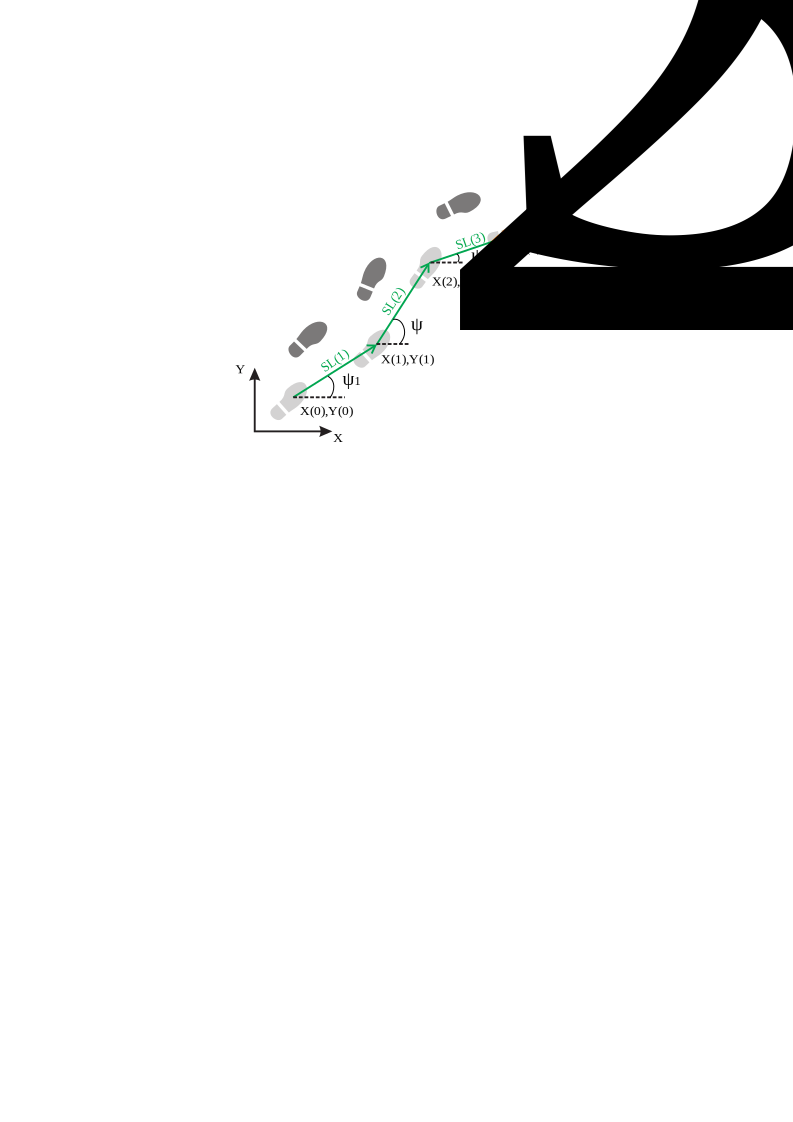
\includegraphics[width=0.8\textwidth]{PDR}
	\caption[A pedestrian trajectory expressed as a concatenation of strides]{A pedestrian trajectory expressed as a concatenation of strides, through their length and orientation. Figure adapted from Francisco Zampella \cite{zampella_localizacion_2017}.}
	\label{fig:PDR_decomposition}
\end{figure}
This formulation based on gait parameters makes the PDR systems to usually be composed of three main blocks: SD, SLE and SHE.
%As it was mentioned in chapter~\ref{cha:1_Introduction}, these systems are also known as step-and-heading systems (SHS) \cite{harle_survey_2013}.

Sometimes, information about the altitude is also necessary. This is the case inside buildings, where knowing the floor may be sufficient. This is usually known as 2.5 dimensional positioning.

% Aunque la definición de muchos de los gait parameters está basada en la posición y movimiento de los pies (entre ellos step length y stride length), la estructura mecánica del cuerpo humano implica que tanto las causas como los efectos del gait cycle estarán distribuidos a lo largo de las diferentes partes del cuerpo.
% Esto significa que deben existir relaciones entre las señales observadas en diferentes partes del cuerpo y los diferentes gait parameters.
% Por tanto, el conocimiento de dichos modelos permitiría diseñar sub-algorithms PDR específicamente diseñados para obtener la longitud y heading de los steps/strides desde  partes del cuerpo específicas.
% Esta es la principal fortaleza de los sistemas PDR: gracias a la naturaleza mecánica del cuerpo humano, los sistemas PDR son flexibles en relación al punto de montaje de los sensores, mejorando así su usabilidad.

% Sin embargo, la obtención de dichos modelos no suele ser sencilla y habitualmente se recurre a modelos biomecánicos o a técnicas de aprendizaje estadístico que obtienen modelos aproximados a partir del análisis previo de un conjunto reducido de instancias del gait cycle.
% Por tanto, la principal debilidad de los sistemas PDR es una falta de generalizabilidad que hace que su rendimiento decrezca cuando las características del movimiento o del subject difieran de los patrones usados durante la creación de los modelos.

Although the definition of many of the gait parameters is based on the position and movement of the feet (including the step length and stride length), the mechanical structure of the human body implies that both the causes and effects of the gait cycle will be distributed throughout different parts of the body.
This means that there must be relationships between the signals observed in different parts of the body and the different gait parameters.
Therefore, the knowledge of such models would allow to design the PDR blocks capable of obtaining the length and heading of the steps/strides from specific body parts.
This is the main strength of PDR systems: thanks to the mechanical nature of the human body, PDR systems are flexible in relation to the mounting point of the sensors, thus improving their usability.

However, obtaining such models is not easy and usually involves biomechanical models or statistical learning techniques. 
In both cases, they obtain approximate models from a previous analysis of a reduced set of instances of the gait cycle.
Therefore, the main weakness of PDR systems is a lack of generalizability that causes their performance to decrease when the characteristics of the motion or the user differ from the patterns used during model creation.

PDR systems can be implemented using different technologies. Some examples include electromyography sensors attached to the calf \cite{wang_novel_2010}, ultrasonic ranging between the feet \cite{saarinen_personal_2004} or the combination of force sensor and ultrasonic transceivers \cite{yeh_geta_2007}.
However, inertial sensors remain the most common technology for the implementation of PDR systems. 
Especially those based on MEMS technology, thanks to their cost, size, weight and their integration in many electronic devices in the market.

% En resumen, para el caso particular de pedestrians y MEMS-based IMUs, INS es el método general y más potentes pero, debido a la calidad de los sensores actuales, la única implementación factible requiere de la utilización de correcciones ZUPT y, por tanto, foot-mounted sensors.
% Por contra, los sistemas PDR ofrecen un interesante compromiso entre usabilidad y adaptabilidad: permiten una mayor flexibilidad en cuanto al punto de montaje del sensor pero su funcionamiento suele estar limitado a un conjunto finito de movimientos (commonly, forward walking and bidimensional positioning) y tipos de usuario.
% Mientras no aumente la calidad de los sensores inerciales para permitir la utilización de INS en más situaciones, los sistemas PDR pueden ser interesantes y suficientes para muchas aplicaciones.

In summary, for the particular case of pedestrians and MEMS-based IMUs, INS is the general and more powerful method but, due to the current quality of that type of sensors, the only feasible implementation requires the use of ZUPT corrections and, therefore, foot-mounted sensors.
In contrast, PDR systems offer a compromise between usability and adaptability: they allow greater flexibility in terms of the sensor's mounting point but their operation is usually optimized to a finite set of motions (commonly, forward walking and two-dimensional positioning) and user's characteristics.
In addition, for both types of systems, the position error is proportional to the number of steps.
For these reasons, as long as the quality of inertial sensors does not increase to allow the use of INS in more situations, PDR systems can be interesting and sufficient for many applications and use cases.

Since inertial PDR systems are the framework for this research work, the following Chapter~\ref{cha:3_pdr_sota} will focus exclusively on reviewing the state of the art of this type of localization systems.
\section{Information Fusion}
\label{sec:2_4_fusion}
In any estimation process, having information from different sources is always positive.
As a general rule, merging several estimates does not always improve the accuracy of the estimate. 
However, the precision of the estimate will always be better than the precisions of the individual estimates.
This may be important for applications that may admit some error in estimation but require certain levels of integrity or confidence in the estimates.
The merging of information can be done from various points of view:
\newpage
\begin{description}
	\item \textbf{Integration of several systems or technologies}
	
	When integrating several localization systems, a first strategy may be to use several systems with similar characteristics, in a redundant manner, such as a foot-mounted INS on each foot \cite{prateek_data_2013} or to combine a foot-mounted INS with a PDR carried in the pocket of the pants \cite{bousdar_ahmed_loose_2017}.
	In this way, the estimation of the position may be improved but the overall system will continue to have the same types of weaknesses.
	
	A fusion strategy that seems more interesting is to combine systems or technologies that have complementary characteristics.
	A simple example in relation to the coverage requirement could be the use of GNSS for outdoors scenarios and WLAN access points for indoors.
	
	However, the most powerful strategy is to merge localization systems based on different methods, i.e. position fixing and DR.
	Remembering the main strengths and weaknesses of each type of method, it can be seen that they complement each other perfectly.
	DR based methods are scenario independent, have a good short-term accuracy but their errors accumulate unbounded over time.
	Meanwhile, position fixing based methods have bounded errors in the long-term but with a risk of temporary higher errors due to interferences or complicated scenarios. In addition, they depend on the infrastructure installed on the scenario.
	
	The most common example of this strategy is the fusion of GNSS and INS systems.
	Furthermore, this integration can be done at different levels, depending on whether only the solutions of each systems is fused (loose coupling) or whether the fusion occurs during the estimation process (tight coupling and deep integration). 
	Detailed descriptions can be found in references \cite{grewal_global_2001, titterton_strapdown_2004, groves_principles_2008}.		

	\item \textbf{Prior knowledge}
		
	Another source of information that can be merged to improve estimates is the available a priori knowledge about the use case, which can be of different types:	
	\begin{itemize}
		\item Information about movement restrictions:
				As previously discussed in Section~\ref{sec:2_3_1_3_DR_INS_ZUPT}, it is possible to use the knowledge about the characteristics of the motion to correct the estimation errors, being two of the best known techniques ZUPT and ZARU, which both make use of the moments when the feet are still on the ground.
				
				Another technique, known as \emph{Heuristic Drift Reduction} (HDR) \cite{borenstein_heuristic_2009}, is to assume that people usually walk in a straight line, especially inside buildings, which allows to reduce the drift in the heading.				
		\item Information about the navigation scenario:
				Having information about the spatial distribution of the characteristics of a certain area is not sufficient to localize an object, but it can be useful to improve the estimation obtained by other means.
				The clearest example is having the map of a building. In addition to assisting in visualization, it can be used to apply corrections to the position estimation, both by using the complete building structure, such as in \cite{woodman_pedestrian_2008, xiao_lightweight_2014, bataineh_conditional_2016}, the detection of landmarks of known position such as stairs, elevators, ramps \cite{jimenez_pdr_2011}, or by the detection of activities performed by the user that may be related to a certain position, such as opening a door.
				
				Similar to the HDR technique mentioned in the previous point, in addition to assuming straight sections in a building, it is also possible to use the ``dominant'' directions of the corridors of a building to correct the heading drift \cite{borenstein_heuristic_2010, abdulrahim_aiding_2010, jimenez_improved_2011, jimenez_improved_2012}. 
				%This technique, and its derivatives, are usually known as \emph{Heuristic Drift Elimination} (HDE) \cite{borenstein_heuristic_2010, abdulrahim_aiding_2010, jimenez_improved_2011, jimenez_improved_2012}.				
				Such techniques will be discussed in Chapter~\ref{cha:9_ihde}.
				
				A more advanced technique is to simultaneously generate a landmark map while locating the object on that map. 
				This technique is known as \emph{Simultaneous Localization And Mapping} (SLAM) and has been widely used in robotics \cite{durrant-whyte_simultaneous_2006}.				
	\end{itemize}	
	\item \textbf{Dynamic estimation}	
	
	The estimation methods for position fixing based localization systems seen in Section~\ref{sec:2_2_2_techniques} assumed that the set of measurements received had been generated when the object was in the same position. This is equivalent to the object being static.
	When the object is in motion, fewer measurements will generally be available at each position, so the estimate will tend to be worse.
	However, it is possible to extend the estimation process by trying to use all the measurements received up to that moment. 	
	For this, it is necessary to have information about the dynamics of the moving object, so that it allows ``linking'' the previous measurements and position estimates with the current one, thus improving the estimation of the moving object.
	
	The mathematical tool that is usually used for this type of information fusion is the Bayesian filtering. 
	Given their importance and frequency of use in the field of localization, the following section introduces the main concepts and techniques.	
\end{description}		
%%%%%%%%%%%%%%%%%%%%%%%%%%%%%%%%%%%%%%%%%%%%%%%%%%%
\subsection{Bayesian Filters}
\label{sec:2_4_1_fusion_bayesian}
The basic idea is to propose that the probability density function of the estimation of the current position of the object, that is, its uncertainty, can be defined as the probability a posteriori conditioned to all the measurements received up to that moment $t$:
\begin{equation}
\label{eqn_bayes_cond}
	p(\boldsymbol{x}_t)=p(\boldsymbol{x}_t|\boldsymbol{z}_1, \boldsymbol{z}_2,...,\boldsymbol{z}_t)
\end{equation}
In general, the complexity of computing such posterior densities grows exponentially over time, since more measurements will be available.
To reduce that complexity, Bayesian filters assume that the dynamic of the system is a Markov process.
Translated to the localization scope, this means that it is possible to make predictions of future positions based solely on the current position, as it contains all the information about its status. In other words, the positions and measurements of the past do not provide additional information.

Under Markov's process condition, it is possible to convert the equation~\ref{eqn_bayes_cond} into an iterative process, based on two phases.
First, the filter predicts the next position from the current estimate of $\boldsymbol{x}_{t-1}$
\begin{equation}
\label{eqn_bayes_pred}
	p^{-}(\boldsymbol{x}_t)=\int p(\boldsymbol{x}_t|\boldsymbol{x}_{t-1})p(\boldsymbol{x}_{t-1})d\boldsymbol{x}
\end{equation}
where $p(\boldsymbol{x}_t|\boldsymbol{x}_{t-1})$ represents the object's dynamic model, that is, how its position varies over time.

The correction phase then merges the newly obtained prediction with the measurements obtained in the period between $t-1$ and $t$. 
By applying the Bayes rule, the posterior probability is obtained as:
\begin{equation}
\label{eqn_bayes_corr}
	p(\boldsymbol{x}_t)=p(\boldsymbol{x}_t|z_t)=\frac{p(\boldsymbol{z}_t|\boldsymbol{x}_{t})p^{-}(\boldsymbol{x}_t)}{p(\boldsymbol{z}_t)}
\end{equation}
where $p(\boldsymbol{z}_t|\boldsymbol{x}_{t})$ is the observation model and the measurement probability $p(\boldsymbol{z}_t)$ normalizes the product for ensuring that the posterior over the entire state space sums up to one:
\begin{equation}
\label{eqn_bayes_norm}
	p(\boldsymbol{z}_t)=\int p(\boldsymbol{z}_t|\boldsymbol{x}^{-}_{t})p(\boldsymbol{x}^{-}_{t})d\boldsymbol{x^{-}}
\end{equation}

In this probabilistic model, $\boldsymbol{x}_{t}$ represents a state vector, so it may contain additional variables to the position such as velocity, orientation or the inertial sensor biases.
In addition, since its formulation is done considering generic probability density functions, it facilitates the fusion of measurements from different types of sensors in a probabilistic way.

The calculation of the different integrals can be difficult to perform in real time. For this reason, there are different simplified implementations of this Bayesian formulation for certain specific cases:
\begin{description}
	\item \textbf{Kalman Filter}

	The simplest case is the \emph{Kalman Filter} (KF), which is based on a state-space representation of the dynamic system in discrete time, and it can be shown that it is the optimal estimator when the error distributions are Gaussian and the observation and dynamic models are linear function of the state vector.
	Although the original derivation of the KF used the orthogonality principle and iterative updates to find the best linear unbiased estimator, it can also be derived using a Bayesian approach, where ``best'' is interpreted in the maximum a posteriori sense, since for Gaussian errors is the same estimate.
	
	So, since a Gaussian distribution is completely described by the mean and the covariance, the prediction stage has the following form:
	\begin{equation} % El & para que se alineen a nivel del =
	\label{eqn_KF_pred}
		\begin{aligned}
			\boldsymbol{x}^{-}(k)&=\boldsymbol{F} \cdot \boldsymbol{x}(k-1)\\
			\boldsymbol{P}^{-}(k)&=\boldsymbol{F} \cdot \boldsymbol{P}(k-1) \cdot \boldsymbol{F}^T+\boldsymbol{Q}
		\end{aligned}
	\end{equation}		
	where $\boldsymbol{x}^{-}(k)$ and $\boldsymbol{P}^{-}(k)$ are the predicted mean and covariance matrix, respectively, $\boldsymbol{F}$ is the state transition matrix and $\boldsymbol{Q}$ is the covariance matrix of the process noise.
	
	The correction stage will use the observed $\boldsymbol{z}$ measurements with its $\boldsymbol{R}$ covariance matrix for modeling the measurement noise:
	\begin{equation} % El & para que se alineen a nivel del =
	\label{eqn_KF_corr}
		\begin{aligned}
			\boldsymbol{x}(k)&=\boldsymbol{x}^{-}(k)+\boldsymbol{K}\cdot (\boldsymbol{z}-\boldsymbol{H}\cdot \boldsymbol{x}^{-}(k))\\
			\boldsymbol{P}(k)&=(\boldsymbol{I}-\boldsymbol{K}\cdot\boldsymbol{H})\cdot \boldsymbol{P}^{-}(k)
		\end{aligned}
	\end{equation}		
	where $\boldsymbol{H}$ is the observation matrix and $\boldsymbol{K}$ is the Kalman constant:
	\begin{equation}
	\label{eqn_KF_K}
		\boldsymbol{K}=\boldsymbol{H}^T \cdot \boldsymbol{P}^{-}(k) \cdot (\boldsymbol{H}^T  \cdot \boldsymbol{P}^{-}(k) \cdot \boldsymbol{H}+\boldsymbol{R})^{-1}
	\end{equation}		
	
	\item \textbf{Extended and Unscented Kalman Filter}	
	
	When some of the KF assumptions, i.e. linearity and normality, are not fully met, modified versions of the KF are usually used which, although sub-optimal, achieve good accuracies.
	
	The first of these is the \emph{Extended Kalman Filter} (EKF), which is based on the linearization of the dynamic and observation models, achieving a similar formulation in which the main difference is the use of the Jacobian matrices of those models, in which only the first terms of their Taylor series are taken.
	
	The other variant is known as \emph{Unscented Kalman Filter} (UKF), which is based on propagating over time a sampling of the mean and covariance of the state vector, which are known as ``sigma'' points. Through this process, states are propagated to the third order terms of their Taylor series, allowing for better estimates and faster convergence.	
	\item \textbf{Particle Filter}
		
	When linearity or normality conditions are not significantly met, non-pa\-ram\-e\-tric filters, such as \emph{Particle Filters} (PF), are often used.
	These filters do not assume any dynamic and observational models and are based on propagating a sampling of the probability distribution of the state vector over time.
	The main objective is to propagate only the most likely points of the sample, eliminating the most unlikely ones in order to reduce the complexity of the calculation.
	This technique is very flexible in terms of the type of measurements that can be used in the observation model, which is why it is usually the technique chosen to include highly non-linear information, such as map-matching information.	
	
\end{description}
There are good references explaining these techniques in detail (KF/EKF \cite{kalman_new_1960,bishop_introduction_2001}; UKF \cite{julier_new_1997};PF\cite{arnaud_tutorial_2008}) and their use in localization \cite{fox_bayesian_2003, seco_survey_2009}.
%%%%%%%%%%%%%%%%%%%%%%%%%%%%%%%%%%%%%%%%%%%%%%%%%%%
\section{Attitude and Heading Reference Systems}
\label{sec:2_5_AHRS}
An \emph{Attitude and Heading Reference System} (AHRS) is like a sub-module of an INS: it only tracks the orientation of the object by integrating the angular rates provided by a set of gyroscopes.
Therefore, in the same way, the orientation error also accumulates over time and information from other type of sensors is usually fused to reduce or reset the error.
Early AHRS designs were based on deterministic fusion strategies and they commonly used accelerometers for reseting the object's tilt, provided that it is static, and magnetometers for the heading \cite{mahony_nonlinear_2008, madgwick_efficient_2010}.
%However, since the use of the values provided by the magnetometers as true heading is mainly restricted to outdoors, last AHRS proposals tend to choose probabilist fusion strategies and limit the use the magnetometers for estimating the gyroscopes bias whenever a constant magnetic field is detected \cite{munoz_diaz_use_2017}.
However, since the use of magnetometers to calculate the actual heading can only be reliably performed outdoors, more recent AHRS tend to choose probabilist fusion strategies and only use such sensors to estimate the bias of the gyroscopes whenever a constant magnetic field is detected \cite{munoz_diaz_use_2017}.

As mentioned in a previous section, the orientation of an object with respect to a reference frame can be represented in several ways: rotation matrix, Euler angles and quaternions.
% Las representaciones son equivalentes pero cada una tiene sus pros y sus contras: 
% \begin{itemize}
	% \item Las matrices de rotación, también llamadas direction cosine matrices, son una matriz de 3x3 cuyas columnas representan la proyección del body reference sobre el global reference. Su principal ventaja es que la matemática de matrices es bien conocida y, además, facilita realizar transformaciones como proyecciones, escalados o traslaciones. Por contra, sus principales desventajas es que no permite visualizar intuitivamente la rotación y que es una representación redundante, ya que utiliza nueve valores para representar tres grados de libertad.
	% \item Leonard Euler demonstrated that the orientation of a rigid body with respect to a fixed reference system can be defined as a sequence of three elementary rotations. Su principal ventaja es que sólo es necesario almacenar esos tres valores y que, conociendo la secuencia de rotación, es sencillo visualizar la rotación total. Por contra, sus mayores problemas son que para operar matemáticamente se deben transformar a matrices de rotación y que algunas secuencias de rotaciones pueden generar una singularidad en la que se pierde un grado de libetad. Esta situación es llamada gimbal lock.
	% \item Los quaternions son una extensión de los números complejos definidos por cuatro parámetros y que permiten representar una orientación como una única rotación alrededor de un eje concreto. Sus ventajas es que son más eficientes que las matrices de rotación y no sufren el problema de gimbal lock de los Euler angles. Sin embargo, tampoco es intuitivo visualizar la rotación a partir de ellos.
% \end{itemize}
These three representations are equivalent as it is possible to convert each one into the others. However, each one has its pros and cons \cite{shuster_survey_1993}: 
\begin{itemize}
	\item The rotation matrices, also called direction cosine matrices, are a three-by-three matrix whose columns represent the projection of the body reference vectors on the global reference. Its main advantages are that matrix mathematics is well known and that it is easy to perform transformations such as projections, scaling or translations. 
	On the other hand, its main disadvantages are that it is not intuitive to visualize the orientation from the matrix expression. Additionally, it is a redundant representation, since it uses nine values to represent three degrees of freedom.
	\item Leonard Euler demonstrated that the orientation of a rigid body with respect to a fixed reference system can be defined as a sequence of three elementary rotations, the so-called Euler angles. 
	The main advantage of this representation is that it is very efficient since only three values are necessary and that, knowing the rotation sequence, it is easy to visualize the orientation. 
	On the other hand, the main problems are that to operate mathematically they must be transformed into rotation matrices and that some rotation sequences can generate a singularity in which a degree of freedom is lost. This situation is called gimbal lock.
	\item The quaternions are an extension of the complex numbers, defined by four parameters.
	They allow to represent an orientation as a single rotation around a particular axis. 
	Their advantages are their numerical efficiency with respect to the rotation matrices and that they do not suffer from Euler angles' gimbal lock problem. 
	However, it is also not intuitive to visualize the orientation from its values.
\end{itemize}
\begin{figure}[!t]
	\centering
	\includegraphics[scale=1]{Yaw_Axis_Corrected_human}
	\caption[Definition of roll, pitch and yaw angles]{Definition of roll, pitch and yaw angles: although there may be variations depending on the definition of the body and global reference systems, in general, the yaw is measured in relation to the vertical axis and indicates the direction that the body faces, the pitch is measured in relation to the lateral axis and indicates the body's elevation, and the roll is measured in relation to the anteroposterior axis.}
	\label{fig:Euler}
\end{figure}
For these reasons, during the mathematical formulation of INS strapdown mechanization, rotation matrices were used.
In contrast, AHRS systems usually use Euler angles when their estimation is to be shown to the user.
So, back to the Euler angles, there are 12 possible rotation sequences, defined with respect to the axes of the body's reference system. 
One of the most common one is the ``ZYX'' sequence, whose three angles are usually known as yaw, pitch and roll \cite{noauthor_ieee_2009}.
As can be seen in the Figure~\ref{fig:Euler}, yaw is the rotation angle around the vertical ``Z'' axis of the body. The term heading is sometimes used as a synonym but it is the angle to the north direction, while yaw is with respect to a reference frame which may not be north-facing.
Pitch, also called elevation, indicates the rotation around the lateral axis ``Y''.
And, finally, the roll angle, also called bank, is around the anteroposterior axis ``X''.
%A visual example of these three Euler angles can be seen in the Figure~\ref{fig:Euler}.
%For this sequence, and as can be seen in the Figure~\ref{fig:Euler}, these 3 angles are usually known as \cite{noauthor_ieee_2009}:
% \begin{itemize}
	% \item Yaw: rotation around the vertical ``Z'' axis. The term heading is sometimes used as a synonym but there is a small difference. Heading is the angle to the north direction. Yaw, on the other hand, is the angle to longitudinal axis of the reference system, which may not be north-facing.
	% \item Pitch: rotation around the lateral axis ``Y''. Also called elevation.
	% \item Roll: rotation around the lateral axis ``X''. Also called bank.	
% \end{itemize}
%\InsertFig{Yaw_Axis_Corrected.pdf}{fig:Euler}{Definition of roll, pitch and yaw angles}{Source: \cite{jrvz_english:_2010}}{0.75}{}
%\InsertFig{Yaw_Axis_Corrected_human.pdf}{fig:Euler}{Definition of roll, pitch and yaw angles}{}{1}{}

PDR systems usually have an AHRS to have a continuous estimation of the heading and, from it, to determine the heading of each step or stride.
In addition, there are also systems that use the Euler angles signals as a source of information for detecting the steps or estimating their length. This is because, depending on where the IMU is mounted, these angles can provide a lot of information about the position of some segments of the human body.
\section{Summary}
\label{sec:2_6_summary}
In this chapter we have reviewed the bases of the two main localization methods: position fixing and dead reckoning.
As explained throughout the different sections, neither is able to offer a perfect solution but, fortunately, their strengths and weaknesses are complementary.
Position fixing methods offer absolute positioning but require the installation of infrastructure, which limits their coverage, and their accuracy will be affected by sporadic interference and complex scenarios.
The DR method is infrastructure-less, which makes it independent of the scenario. However, it only offers relative positioning and its great limitation is the unbounded accumulation of error over time.

\begin{figure}[!t]
	\centering
	
\includegraphics[width=0.8\textwidth]{seamless_architecture_2}	
	\caption{Conceptual architecture of a seamless localization system}
	\label{fig:architecture}
\end{figure}
The techniques of information fusion, besides allowing to combine both methods of localization, also allow to merge a priori known information about the scenario or the nature of the movements of the object to be positioned.
It is even possible to merge the position estimates of other mobile nodes, in what is known as cooperative or network localization \cite{wymeersch_cooperative_2009}.
Therefore, it seems logical to think that the architecture of a system capable of providing localization information seamlessly should integrate all these elements, as represented in the Figure~\ref{fig:architecture}.
However, the cooperative localization, the a priori information and the position fixing methods should be considered as opportunistic, as it cannot be assumed that they will always be available.
This does not happen with DR based methods, which will work continuously, so they should be considered as the basis of a seamless localization system.

Therefore, when implementing a system with these characteristics for pedestrians, the use of wearable devices that include inertial sensors seems mandatory.
Among them, wrist-worn wearables, such as smartwatch and smartbands, stand out for their availability on the market and their convenience for users.
%\InsertFig{seamless_architecture.pdf}{fig:architecture}{Conceptual architecture of a seamless localization system}{}{1}{}


% background
% this file is called up by thesis.tex
% content in this file will be fed into the main document



% this file is called up by thesis.tex
% content in this file will be fed into the main document

%: ----------------------- introduction file header -----------------------


\begin{savequote}[50mm]
The good thing about science is that it's true whether or not you believe in it. 
\qauthor{Neil deGrasse Tyson}
% The beginning is the most important part of the work.
% \qauthor{Plato}
\end{savequote}


\chapter{Background}
\label{cha:2_background}

Amidst the surge of vast streaming data, governments and businesses find themselves in an urgent need for sophisticated data analysis and machine learning analytics approaches. These tools are indispensable for anticipating future trends and making well-informed decisions. However, the perpetual emergence of new goods, markets, and consumer behaviors introduces a formidable challenge known as concept drift [24]. This phenomenon involves the variation of statistical parameters of the target variable over time in unexpected ways, posing a substantial obstacle to accurate forecasting and optimal decision-making. The patterns derived from historical data may become obsolete when applied to new and evolving datasets.
The impact of concept drift extends across data-driven information systems, including decision support and early warning systems, diminishing their overall effectiveness. In the dynamic realm of big data, where data types and distributions are inherently unpredictable, the challenge of concept drift becomes even more pronounced. In response to this challenge, the field introduces a new subject: adaptive data-driven prediction/decision systems.

\section{Data Preprocessing}
\label{sec:2_1_DP}

Data preprocessing \cite{garcia2015} includes data preparation; (e.g., integration, cleaning, normalization, transformation) and data reduction; (e.g., instance selection, feature selection, discretization). The desired result is to get a cleaned, relevant, manageable, and meaningful dataset ready for analysis. Usually, there is a trade-off between time-complexity and accuracy to get the prepared data, which keeps the research ongoing for this area. 
\vspace{7mm}

\noindent \textbf{Data Preparation:}
Refers to a set of techniques to prepare data as an input for a certain DM algorithm. Usually, it is ignored by inexperienced practitioners, which may cause the model runtime crash. Even if the algorithm works, the expected results will not be optimistic. A set of preliminary steps can be followed before model training as described in \cite{garcia2015}: 
\begin{itemize}
    \item[-] \textbf{Data Cleaning:} The process of detecting and correcting (or removing) inaccurate records from data. Other tasks could be to detect irrelevant data fragments that do not make sense. The result will be a consistent, accurate, meaningful dataset \cite{rahm2000d}.
    
    \item[-] \textbf{Data Transformation and Data Integration:} Data transformation is the process to convert and consolidate the data to another format to improve model efficiency. This process is composed of sub-tasks; feature construction, feature aggregation, normalization, and more. While data integration is recommended for merging data that come from multiple data sources. The aim is to detect conflicts and to remove redundant and inconsistent data \cite{lenzerini2002,doan2012}. 
    \item[-] \textbf{Data Normalization:} This process is dedicated to unify the measurement unit to all the attributes. Under this schema, all the attributes are equally weighted. Statistically, to align the entire probability distribution of the adjusted values, to reduce the effects of certain gross influences \cite{pochon2008,pyle1999}.
    
   \item[-] \textbf{Missing Data Imputation and Noise Identification:} Training a model with a dataset that has many missing values can have a dramatic effect on the quality of the machine learning model. The imputation strategies can be (Mean/Median values, most frequent value, k-nearest neighbors, using deep learning, multivariate imputation by Chained Equation) \cite{buuren2010}. Noise identification is known as smoothing, to detect variances or random errors in a measured variable \cite{wang2010}. 
\end{itemize}


\noindent \textbf{Data Reduction:}
Not like data preparation, data reduction is an optional step. It provides a set of methods for obtaining a reduced version of the original data. It is the process of downsizing the data while maintaining the integrity of the complete dataset. However, it could be a crucial step as data preparation, to enable the DM algorithm when the data size exceeds. Following are some representative approaches: 

\begin{itemize}
    \item[-] \textbf{Feature Selection:} Data reduction can be accomplished by removing irrelevant or redundant attributes. The aim is to use the least number of features while keeping the output of the classification as similar as possible as if we were using the full feature set. Regarding that, the training speed can be boosted and the model performance can be elevated \cite{li2017, dash1997}. 
    \item[-] \textbf{Feature Extraction:} Lessening the amount of resources required for the representation of a large array of data. Analysis with a wide range of variables usually involves a large amount of memory and computational resources. In addition,  the classification algorithm could generalize to new samples badly. Feature extraction is a set of techniques that create combinations of variables to fix these issues, but also reflecting the data with sufficient precision. Many machine learning specialists believe that the properly configured extraction of features is the key to a successful model building \cite{geron2019}. 
    
    \item[-] \textbf{Instance Selection:} The process of reducing or eliminating samples intelligently without affecting the DM application. This process can be guided by heuristic rules to select horizontal subsets of data \cite{olvera2010,fu2013}. In addition, the process can be applied to adapt with a particular DM algorithm; like "selection of support vectors for support vector machine algorithm" \cite{liu2017}.   
      \item[-] \textbf{Discretization:} The mechanism by which quantitative data is converted into qualitative data; via converting numerical variables into discrete or nominal variables. For that, a huge spectrum of numeric values can be compacted or reduced into a subset of discrete values \cite{ding2010}.  
\end{itemize}

Finally, the benefits of data preprocessing can be among the following; (1) Adaptation to a particular machine learning algorithm. (2) Increasing predictive accuracy. (3) Enabling: data mining algorithms are negatively affected by the data size, and data reduction provides a solution for data choking. (4) Cleaning noisy, missing, and redundant data to improve data quality. (5) Focusing: to focus on relevant data instead of all available information.


%%%%%%%%%%%%%%%%%%%%%%%%%%%%%%%%%%%%%%%%%%%%%%%
%
%   Brief history of TF
%
%%%%%%%%%%%%%%%%%%%%%%%%%%%%%%%%%%%%%%%%%%%%%%%
\section{Data Mining}
\label{sec:2_2_SML}
A closely related field to machine learning is Data Mining, which is defined in \cite{lantz2013} as, "\textit{the generation of novel insights from large databases}". While in \cite{garcia2015}; data mining is defined as, "\textit{solving problems by analyzing data present in real databases}". While others \cite{chakrabarti2006,han2011,nisbet2009,clifton2010} view DM as, "\textit{the main steps of knowledge discovery in databases}". The main distinction between ML and DM is that; ML is dedicated to teach computers how to use data to solve problems, while DM is dedicated to teach computers how to identify patterns like a human to solve problems. It is interesting to mention that every DM involves the use of ML, but not all ML involves DM. Next, a brief description of data mining categories is presented:
 
\begin{itemize}
    \item [-] \textbf{Unsupervised Learning}: Those techniques deal with an unlabeled dataset, with a minimum of human intervention \cite{fisher2014}. Data with no pre-existing labels at our disposal and the purpose is to find associations, relationships, regularities, and similarities in the data. Cluster analysis is among the common models used in unsupervised learning. Cluster analysis is the process to segment/group datasets with shared attributes \cite{kaufman2009}. Unlabeled examples are given an implied cluster label from the relationships within the data entirely. Sometimes, the clustering task is referred to as "unsupervised classification", because it classifies unlabeled examples.   
    
    
\item[-] \textbf{Supervised Learning:}   Supervised learning is popular in the field of DM, commonly knows as prediction methods. In supervised learning, a relationship is to be learned between input space and target space. Based on the predicted target type, there are two common tasks; regression and classification. In regression, the numerical output to be predicted falls in a certain interval. Contrary to classification, the domain of the target is finite and categorical.   
\end{itemize}

    



Next, all the subsequent sections will be dedicated to the classification task in matching with the core of this thesis. In the classification problem, the input attributes (features) and the target attribute (class) are transparent. The aim is to learn a function that maps inputs to outputs. The learned function is called a model, and it is inferred from labeled training data. Let, 

\begin{equation}\label{eq:classification}
\textbf{x}=\left[x^{(1)},..., x^{(d)}\right]^T,\textrm{ and } \textbf{x}\in \mathcal{X}=\mathcal{X}^{(1)}\times ... \times \mathcal{X}^{(d)}
\end{equation}
 
\noindent where $\mathcal{X} $ denotes feature space and \textbf{x} is the sample, i.e., \textbf{x} is the so-called feature vector which informs about attribute values. We will assume that we have $d$ attributes at our disposal. The supervised classification model will assign a given object described by its features, \textbf{x}, into one of the predefined categories, also called labels. Let $\mathcal{M}=\{1,..., M\}$ stands for the set of class labels (decision regions). The classification algorithm (discrimination algorithm) is any learned function $\Psi$ with domain $\mathcal{X}$ and codomain $\mathcal{M}$ as clarified in Equation (\ref{mapper}). Where the target values in codomain are finite and categorical.  

\begin{equation}\label{mapper}
\Psi\: :\: \mathcal{X} \to \mathcal{M}.
\end{equation}

\begin{figure}[!ht]
    \centering
    \includegraphics[width=\textwidth]{2_Background/figures/fig_SML_models.pdf}
    \caption{Supervised classification algorithms.}
    \label{ch2:cl.sml}
\end{figure}

There is a large number of models with different inferring strategies to discover the hidden patterns from data. Next, I provide a short review of popular classification algorithms according to the division in Figure \ref{ch2:cl.sml}, inspired by \cite{garcia2015}.  

\begin{itemize}
    \item Regression Models: Logistic Regression (LR) is a statistical model, that returns a probability for each class level. The cutoff value is embedded to separate the upper and the lower probabilities to work as a binary classifier (binomial LR). While multinomial LR deals with more than two classes. In order to be enabled, the missing values should be handled. In addition, the high correlation among the predictors (variables) should be minimized. LR has been praised for its robustness and simplicity \cite{friedman2001}.  \item Artificial Neural Networks (ANNs): The excessive and growing formulations of ANNs from the theoretical and algorithmic depth \cite{carlini2017}, made them more influence on the field of pattern recognition. ANNs handle large and complex tasks due to their nested non-linear structure. While non-explanation is one of the pitfalls of those black-box models.  The computations of those models are based on the definition of neurons. ANNs are unstable and more sensitive to small changes in training data. Similar to LR, they require no missing values.  
    \item Bayesian Learning: Based on the probability theory to get rational decisions \cite{saritas2019}. The Na\"ive Bayes is the most popular algorithm in this category. The posterior probability for each class label is calculated, then the decision is promoted upon the maximum probability returned. Those methods only work with categorical attributes, cannot work with missing values, and are very sensitive to redundancy. The "Na\"ivety" comes from the assumption of the conditional independence between features. It can be viewed as an explainable model to give reasoning about the decisions. 
    \item Instance-based Learning: The prediction of a new unknown sample is based on a distance function with the past stored samples. Also called memorization techniques and lazy learners \cite{lopes2015}. The performance of those methods is affected by the used distance function, neighborhood size, and decision aggregation mechanism. K-Nearest Neighbor (KNN) is the most popular method in this category. Pitfalls of those methods can be mentioned as: high memory space for storage, delayed prediction response, sensitivity to noise.
    \item Support Vector Machines (SVM): Learning algorithms which are based on maximizing gab separation (margin) between different class samples to get correct decisions. They are suitable to work as linear and non-linear data separation. Only the class borders (support vectors) are important to optimize the margin where internal points can be removed to improve the efficiency \cite{nalepa2019}. They require no missing values and are commonly robust against noise. \item Rule Learning: Called divide-conquer algorithms \cite{furnkranz2012}. The data parts are divided based on one rule, then recursively conquer the divided parts. Those models are transparent or explainable to nonexperts in the form of logical structures. Available features are analyzed to find homogeneous groups, then an additional rule is built to drill down more. Small changes in the training data results in decision change. Rule learning techniques are affected by missing values, noisy samples, and outliers.
    \item Decision Trees (DT): This is a kind of indirect rule learning. Uses structure branching decisions to model the relationships among the features and the predicted class value. They are widely used and can model any type of data. The human-readable model is appropriate in applications where legal reasoning is required. Those models are vulnerable to overfitting, and the internal parameters should be tuned \cite{geron2019}. Unstable like ANNs and sensitive to change in the training data. Usually, they are biased towards the splits on features.               
\end{itemize}

For unseen pattern $\textbf{x}$, a class membership values are calculated as in Equation (\ref{membership}), then the labeling choice will be connected to the highest score.
\begin{equation}\label{membership}
\Psi(\textbf{x})=\text{Max}\{g_1(\textbf{x}),g_2(\textbf{x}),\dots,g_M(\textbf{x})\}
\end{equation}


 The decision region $R_1$ for the $1^{st}$ class, is the set of points for which $g_1(\textbf{x})$ has the highest score \cite{kuncheva2014}. While the \textit{classification boundaries} contain data points for which the membership values tie. If the decision region $R_1$ contains data points from the $2^{nd}$ class, then we have overlapped classes. From Figure \ref{ch2:overlapping}. (c) and as shown in \cite{galbusera2019}, the regions are nonoverlapping as the model learns all the details about the data. This case is known as overfitting, and the model will not perform properly to predict unseen samples. While  Figure \ref{ch2:overlapping}. (a) shows the optimal class separation boundary that guarantees minimum possible error with the future samples. Finally,  Figure \ref{ch2:overlapping}. (b) shows the the underfitting case when the model fails to capture relationships between a dataset’s features and a target variable during training. 
 
 
 \begin{figure}[!ht]
    \centering
    \includegraphics[width=\textwidth]{2_Background/figures/fig_overlapping.pdf}
    \caption{Trade-off between overlapping and overfitting, taken from \cite{galbusera2019}.}
    \label{ch2:overlapping}
\end{figure}


Each model has an accompanied error, we need to understand the different sources that cause this error. Equation (\ref{Gen.error}) represents the compound generalization error $E_G$ of a classifier $\Psi$ that is trained on dataset $D$. 


\begin{equation}\label{Gen.error}
E_G(\Psi,D)=E_A(D)+ E_M+E_B
\end{equation}

\noindent where $E_A(D)$ is the "approximation error" represents the variance due to using different training data, or non-deterministic training algorithm. Clarified as, the hyper-parameters of the model that affect its performance. The second term $E_M$ is the "model error" which represents the bias due to selecting a model in preference of another. The last term $E_B$ is the "irreducible error" coming from the insufficient representation of the data. This is commonly known as Bias/Variance Tradeoff \cite{geron2019,kuncheva2014}. Increasing a model’s complexity will typically increase its variance and reduce its bias.
Conversely, reducing a model’s complexity increases its bias and reduces its variance.
This is why it is called a tradeoff.    
%%%%%%%%%%%%%%%%%%%%%%%%%%%%%%%%%%%%%%%%%%%%%%%
%
%   Machine Learning Modelling Approaches of Traffic Forecasting
%
%%%%%%%%%%%%%%%%%%%%%%%%%%%%%%%%%%%%%%%%%%%%%%%
\section{Ensemble Data Mining}
\label{sec:2_3_EDM}

Ensemble learning is the strategy of using multiple learning algorithms in order to obtain greater predictive precision than all of the constituent learning algorithms alone \cite{polikar2006,polikar2012,rokach2010,dietterich2002,zhang2012,opitz1999,sagi2018,oza2001,krawczyk2017}. In addition, Wozniak. et al. defined ensemble models as hybrid intelligent systems \cite{wozniak2014} with the potentiality to cope with ambiguity, uncertainty, and complex problems. Thanks to their capabilities, ensembles received great attention in the applications related to data mining. For unsupervised learning, clustering performance could be significantly improved by ensemble methods \cite{zhou2006,vega2011,cornuejols2018}. Furthermore, ensembles are employed for unsupervised anomaly detection \cite{zhao2015}. While, for supervised learning, those systems are widely popular for regression tasks \cite{mendes2012,ren2015} and for classification tasks \cite{wozniak2014,sagi2018}.


Ensemble systems for pattern classification have been expanded in the literature under creative names as: consensus aggregation \cite{benediktsson1992}, stacked generalization \cite{naimi2018}, committees of neural networks \cite{cirecsan2011}, mixture of experts \cite{jacobs1991,jordan1994}, classifier ensembles \cite{yu2014,rodriguez2006}, classifier selection \cite{ruta2005,cruz2018}, multiple classifier systems \cite{wozniak2014, catal2017}, classifier fusion \cite{liu2017cl} and more.  Theoretical and empirical studies prove that ensemble systems are more accurate than any random classifier \cite{catal2017, tahir2012,polikar2006,fernandez2014}. The final decision is the accumulative decisions of all the classifier set. Let $\Pi$ denotes a pool of $T$ base classifiers $\Pi=\{\Psi_1, \Psi_2,\Psi_k ..., \Psi_T\}$ to be grouped by a combination function. The ensemble output $\hat{\Psi}$ is determined on the basis of the outputs of the base classifiers, i.e.,

\begin{equation}
\label{eq-generalfusion}
\hat{\Psi}(\textbf{x})=F(\Psi_1(\textbf{x}), \Psi_2(\textbf{x}), ..., \Psi_T(\textbf{x}))
\end{equation}

\textit{Intuitively, any classifier ensemble is in fact a classifier} (L. Kuncheva \cite{kuncheva2014}).


% \begin{figure}[!ht]
%    \centering
%    \includegraphics[width=.7\textwidth]{2_Background/figures/fig_ensemble-top.pdf}
 %   \caption{The simple topology for combining classifiers, taken from \cite{kuncheva2014}.}
  %  \label{ch2:ensemble-topology}
%\end{figure}










Each learning algorithm, Section \ref{sec:2_2_SML}, has a limit to discovering the hidden pattern. According to Wolpert's \emph{no free lunch} theorem \citep{wolpert2002}, there is no best classifier suitable for all problems, but each model has its own area of competence giving the design assumptions. For that, a set of learning models solving the same problem can be consolidated to generate a better composite global model \cite{ksieniewicz2018}. L. Kuncheva \cite{kuncheva2014} stated \textit{"the improvement of the ensemble over the single best classifier or even on the average of individual classifier accuracies is not guaranteed"}. From our perspective, the proper design of ensemble is conditioned by outperformance over the best individual classifier in the group.  



\subsection{Are we pursuing complexity?}
Why we accept complex systems instead of depending on a single classification algorithm?. The answer to this question is highlighted in the following points.
\begin{itemize}[nosep]
    \item[-] Ensemble models are the solution to deal with uncertainty. A solution from a single classifier can be boosted and trusted by aggregating a group of predictors (\textit{wisdom of crowds} \cite{rokach2010}).
    \item[-] There is no guide to design universal approximators, perfect model, i.e. it is difficult to set up ANNs or reaching their optimistic parameters.

    \item[-] Ensemble selection or pruning is an interesting research topic that aims to reduce ensemble complexity without deterioration in the performance.
\end{itemize}

In addition, a promising solution via ensemble learning can be achieved for the following scenarios:

\begin{itemize}[nosep]
    \item Imperfect Learning: Non-deterministic classifier can be considered as a local optimizer in terms of the training error, a safer option is to group several models that cover the solution space properly.
    \item Too much data: We are surrounded by too much data. In this case, data is split into chunks where similar or different learning algorithms can be trained on each part independently. Ensemble learning support parallelization and distributed computing for handling this scenario efficiently.
    \item Small-size data: In data shortage, stratified sampling with replacement can be applied, where several data replications will be obtained to train individual classifiers inside the ensemble. 
    \item Data fusion: The data pattern can be identified differently based on the data source. The availability of sensors strengthens decision making by analyzing different features. Instead of fusing all features and building a single classifier, it could be better to build a single classifier for each feature space and combine their decisions.  
    \item Complex hypothesis: Complex classification boundary can be approximated by combining several base classifiers.
    
\end{itemize}


\subsection{A Taxonomy of Classifier Ensemble Methods } \label{ch2.taxonomy}

A comprehensive review of the classifier ensemble methods, thorough discussion, and the development of further knowledge in this area was the core of many articles \cite{gonzalez2020,polikar2006,cruz2018, britto2014,re2012,sewell2008}, with a proposed taxonomy by L. Rokach \cite{rokach2009} who indicated the five dimensions to design this kind of powerful models. Figure \ref{ch2:ensemble-taxonomy} shows our perspective for the Multiple Classifier System (MCS) taxonomy as it has been proposed by L. Kuncheva \cite{kuncheva2014}, R. Cruz et al. \cite{cruz2018}, and L. Rokach \cite{rokach2009}. The two main phases in classifier ensembles are; Generation and Integration, while the selection is an intermediate/optional phase.   

\begin{figure}[!ht]
    \centering
    \includegraphics[width=.95\textwidth]{2_Background/figures/fig-taxonomy.pdf}
    \caption{The Taxonomy of Multiple Classifier System (MCS).}
    \label{ch2:ensemble-taxonomy}
\end{figure}



\subsubsection{Generation} \label{sub.generation}
The goal in this phase is to generate a pool of classifiers that are both diverse and accurate. This phase discusses strategies to handle data horizontally/vertically. In addition, what classifier type to accommodate, how to build the classifiers: dependent/independent manner, and how many classifiers to train (ensemble pool size). 

 \textbf{1) Diversity:}
Diversity is one of the main reasons for the effectiveness of ensemble methods \cite{zhou2012,gonzalez2020}. Diversified classifiers cause uncorrelated errors, which lead to improved classification accuracy \cite{hu2001}. In general, this can be achieved through the following six wide subcategories to promote diversity during the generation phase.
\begin{itemize}
    \item[-] \textbf{Different Parameters/Initialization:} \textit{Algorithm-level diversity}; via different parameters, the base classifiers can be generated by modifying the hyper-parameters of the learning algorithm; for example, controlling the number of $k$ neighbors, distance function in KNN model, and controlling the confidence level parameter in the decision tree. While, via different initialization and if the training process is initialization dependent, the model will be sensitive. In neural networks, different initial configurations of weights result in different decisions \cite{hansen1990}.        
  \item[-] \textbf{Different Architectures:}  \textit{Algorithm-level diversity}; this strategy is more suitable to multi-layer perceptron neural networks, where the number of hidden layers, the number of neurons, and the network topology affect the classifier domain space. For example; in the Addemup algorithm \cite{opitz1996}, the genetic algorithm is used to choose the required network topology to compose the ensemble according to a measure of diversity.     
  \item[-]\textbf{Different Classifier types:} \textit{Algorithm-level diversity}; each classifier model build its inference with a capability to discover a hidden pattern differently. Each model, Section \ref{sec:2_2_SML}, contains explicit or implicit bias that leads to a better generalization accuracy through combination. In addition, as in \cite {woods1997}, the divide and conquer mechanism is best implemented by calculating the local accuracy in the feature space to choose between four different classifier types.  
  \item[-]\textbf{Data Partitioning:} \textit{Data-level diversity}; Partitioning means the division into smaller disjoint components of the initial training. A different classifier will be trained on each part to gain different and accurate decision \cite{maimon2005}. This mechanism enables data mining algorithms to handle massive datasets by managing memory size and computational resources perfectly. The data can be partitioned horizontally or vertically. \textit{In horizontal partitioning}, several parts will be formed; each part will contain sub-samples while sharing the complete feature set. Sub-samples can reflect the entire dataset by selecting the instances from all the formed clusters of the dataset; known as cluster-based concurrent decomposition (CBCD) \cite{rokach2005}. The mixture of experts (ME) \cite{nowlan1991}   splits the input space into several subspaces and assign an expert, classifier, to each subspace. In \cite{cohen2007} a decision tree framework is employed to divide the input space into mutual exclusive partitions, then a new unseen pattern will be classified by a dedicated classifier that is learned from the space to which the instance belongs. \textit{In vertical partitioning}, The feature space is partitioned into several subsets keeping the same number of samples, then each classifier can be trained on a different projection. This mechanism is more suitable for a high-dimensional dataset without affection by the feature selection drawbacks \cite{tumer2003}, and the accuracy could be improved by the less correlation among classifiers. This division results in a high-speed classification algorithm \cite{bryll2003}, and solves the problem of class under-representation that exist with instance-based sampling.      
  
  \item[-]\textbf{Resampling:} \textit{Data-level diversity}; the diversity could be promoted by manipulating the training set. Each base model is trained over a different sample from the training. Bagging \cite{breiman1996,skurichina1998} and Boosting \cite{freund1997,freund1999} are the popular strategies in that paradigm. Bagging ensembles achieve a reasonable diversity level by creating different bootstrap samples to train each base model independently, then the final decision is adopted by a simple majority voting-based aggregation. Moreover, the non-sensitivity of bagging and robustness under diverse noise conditions makes it more attractive \cite{dietterich2000}. Contrary to sequential ensembles, \textit{Boosting}, the individual members are generated in the sequential schema by the learning algorithm \cite{freund1997}. The sequential mechanism of boosting encourages the complementariness between ensemble members, by focusing on previously misclassified samples. However, the performance in boosting is more sensitive to noisy samples \cite{dietterich2000,caruana2006} and sometimes overfitting can be observed for large pool size \cite{ratsch2001}. 
  
  \item[-]\textbf{Differnet label targets:} \textit{Data-level diversity}; manipulating the target attribute is very interesting mechanism to promote diversity. Instead of building complex classifier, several classifiers with usually simpler representations, about the target attribute, will be trained. For instance, to handle the multi-class dataset, the original target attribute can be replaced by a simpler and smaller target domain. Among those strategies, One versus all (OVA) \cite{anand1995} which divides the $M$-class classification problem into $M$ two-class classification tasks. While one versus one (OVO) \cite{lu1999} divides the $M$-class classification problem into $M(M-1)/2$ two-class classification tasks, so the complex decision boundary can be simplified. Minimal classification method (MCM) \cite{sivalingam2005} converts the $M$-class classification task to the minimal binary classification tasks. MCM requires $\log_2(M)$ classification tasks in the form of a separation between groups of multiple classes. Furthermore, the error-correcting output coding (ECOC) algorithm, uses a code matrix to decompose the multiclass problem into multiple binary problems \cite{dietterich1994}. In addition, label switching algorithms \cite{breiman2000,martinez2005} change the labels of samples picked randomly. 
\end{itemize}


\textbf{2) Building:}
This part discusses the building schema to generate a pool of classifiers, whether to be dependent or independent. In the dependent framework (sequential/incremental), the performance of a classifier affects the creation of the next classifier in the chain. Instead, in the independent framework (simultaneous), the classifiers are generated independently. 

\begin{itemize}
    \item[-]\textbf{Simultaneous:} The independent methods to generate a set of classifiers mainly depends on forming different training samples from the original training set. The training samples could be mutually exclusive (disjointed) or overlapping. The reason behind preferring this schema is to improve the predictive accuracy or to speed up the generation step as this schema supports parallel implementation. \textit{Bagging} (Bootstrap AGGregatING) \cite{breiman1996} is the popular method in this category, with a replacement from the original training set, each classifier is trained on data samples. The sample size will be equivalent to the original training size; randomly some samples will be duplicated and some samples will be ignored.  
     \item[-]\textbf{Incremental:} Sometimes called dependent, there is a kind of interconnection during the learning process. The model generation depends on the accuracy of the previous model/committee. The training process is done in iterative form, where the learning process will be directed to focus on the previously misclassified samples. \textit{Boosting} \cite{freund1996} (also known as arcing- Adaptive Resampling and Combining) is the popular method in this category. The training process mainly depends on assigning weights to all the training samples. In the beginning, all the samples will be equally weighted (having the same importance), but throughout the iterations, the weights of correctly classified samples are lowered while the weights of misclassified samples are raised. As a consequence, the base model is directed to focus on the hard samples in the training set.          
\end{itemize}


\textbf{3) Universality:}
This part discusses the universality of the ensemble model. Some ensembles techniques could be designed to work for any classifier, while other ensembles have been designed to work with specific classifiers. In other meaning, the relation between the ensemble technique and the used classifier type. 

\begin{itemize}
    \item[-]\textbf{Specific Inducer:} Known as inducer-dependent ensembles, where the effectiveness of the ensemble could be degraded if applied for other classifier types. For example, \cite{hansen1990,lu1999} those ensembles are explicitly designed for neural networks. Additional schemas \cite{tao2006} are perfectly suited for SVM.
    
     \item[-]\textbf{Any Inducer:} Known as inducer-independent ensembles, Those implementations can be extended to a wide variety of classifier types without affecting the generalization accuracy. 
    
\end{itemize}


\textbf{4) Ensemble Size:}
This part discusses the aspect of pool size. How many classifiers should be trained?. The main four factors that concern the ensemble size as determined by L. Rokach \cite{rokach2009} are; (A) \textit{Sufficient Accuracy}; the appropriate accuracy of the ensemble could be reached by aggregating 10 models \cite{hansen1990}, while other empirical studies show that this level of accuracy is correlated with large-size ensembles containing 25 models \cite{opitz1999}. (B) \textit{Computational Cost}; the more classifiers are generated the more computational resources are consumed. As a consequence, the user may predetermine the pool size to match the computational cost limits. (C) \textit{Nature of Task}; the ensemble size could be problem-dependent, as we stated before with the ensemble size of OVO and OVA strategies for handling multi-class classification tasks. (D) \textit{Number of processor cores}; for independent ensembles, the number of internal cores can be the upper bound to control how many classifiers can be trained in parallel mode.                      

\begin{itemize}
    \item[-]\textbf{Fixed in Advance:} This is the simple form to predetermine how many iterations should be considered. Most Bagging and Boosting software packages give the flexibility to control the number of iterations.  
    
     \item[-]\textbf{Determined during Training:} The best ensemble size can be determined during train time. The contribution of a new classifier to the ensemble performance is to be checked if it is significant or not. To estimate the unbiased error of the test sample, Random Forests uses the out-of-bag (OOB) procedure. The OOB error estimation is used in \cite{banfield2006} to determine the sufficient number of classifiers. As the maximum accuracy no longer increases, the training procedure stops.       
    
\end{itemize}



\subsubsection{Selection}
There is no value from combining similar classifiers' decisions. The effectiveness of the ensemble is conditioned by the diversity and the correctness of the base classifiers. Ensemble Selection is one of the strategies that can be used to handle this challenge. Ensemble Selection has been known in the literature as ensemble pruning \cite{lu2010,zhang2006,ykhlef2017}, ensemble thinning \cite{banfield2005} and ensemble reduction \cite{diao2013,zhang2018}. ES can be considered as an intermediate process between building the ensemble and aggregating the decisions. Specifically, ES is the strategy of optimizing and selecting the number and the type of individual classifiers in-advance. Collecting the decisions from a reduced number of models speeds up the classification systems and relieves memory storage. In the literature, the selection process can be performed offline, static selection \cite{tsoumakas2009}, or online, dynamic selection \cite{cruz2018}.
 
 
 \begin{itemize}
    \item[-]\textbf{Static Ensemble Selection:} Known in the literature review as ensemble pruning. This process is done during the training and before the real test. A subset of classifiers that optimize a predefined function/metric are selected, and the estimation of that metric is done over a pruning set. The most common metrics/selection criteria are; diversity \cite{aksela2003,brown2010}, classification accuracy \cite{dos2009,ruta2005}, instance margin \cite{yang2012, guo2013,hernandez2008}. However, it is not trivial to find the optimal subset of classifiers from a large ensemble as the complexity increases exponentially with the pool size. Researchers agreed in common that ES is a combinatorial search problem with $2^{T}-1$ nonempty subsets to be evaluated from pool size, $T$, to find the best subset \cite{tamon2000, tsoumakas2009}. To handle this complexity, several attempts ranging from optimized search \cite{diao2013,adnan2016,ruta2001b}, clustering techniques \cite{onan2017,zyblewski2020}, and greedy algorithms \cite{cao2018,martinez2009,margineantu1997, partalas2010, mao2011} have been applied over decades. More details about ordering-based pruning will be discussed in Section \ref{ch5_ordering_pruning}.        
    
     \item[-]\textbf{Dynamic Ensemble Selection:} This process is done during the test time. A single classifier or subset of classifiers are selected based on the unseen sample. In addition, dynamic weights are assigned according to the competition among individual classifiers over the local region of an unknown sample $\textbf{x}$. As a consequence, the selected subset is changeable for each test pattern \cite{KO2008}. This process consists of three steps; (1) Definition of the local region surrounding the query sample $\textbf{x}$, (2) Determination of the selection criteria to estimate the competence level of the classifiers, and (3) Determination of the selection mechanism, whether to select a single classifier or ensemble of classifiers. Without debate, dynamic selection techniques can outperform the static selection methods as experimentally been proved in \cite{cruz2018} since the selection is optimized for each test sample independently. The rationale in dynamic selection is that each classifier is an expert in a different local region within the feature space. However, in the dynamic selection, there is a computational overhead for selecting subensemble for each test sample. Besides, those techniques flood the memory space as all individual classifiers have to be retained in memory. Additionally, the dynamic selection is affected by the outlier instances around the query sample in the feature space \cite{CRUZ2015}.
    
\end{itemize}

Cluster and pick \cite{kuncheva2000} is a poor variant of dynamic selection. Initially, the input space is split into disjoint regions via clustering the training samples. The best classifier is then defined and chosen for each cluster. Cluster and select is in-between static and dynamic strategies; the classifiers are selected dynamically depending on which region the input sample belongs to, but the regions are static, determined in advance during the training \cite{ruta2005}.

 
 
 
\subsubsection{Integration}
Also known as the combiner function. The combiner balances the deviation between the diversity and the bias, also alleviates the errors that certain models have made \cite{SOARES2013}. This process concerns the methodology by which the outputs of the base classifiers will be aggregated.  A vital phase in building a group of classifiers is the use of a suitable fusion strategy to aggregate response decisions \cite{zhou2012,kuncheva2014}. The responses of individual classifiers restrict the fusion method and enhance or degrade the composite prediction. Those responses may be on the \textit{abstract level} \cite{xu1992}, where each classifier specifies a class name as a decision. Additionally, the responses may be \textit{ranked levels} \cite{PARKER2001}, where each classifier outputs a ranked subset of class labels, or even  \textit{measurement values} \cite{kuncheva2014a,niu2007}, where each classifier specifies a posterior probability.


\begin{itemize}
    \item[-]\textbf{Non-trainable:} 
    The combination function does not require any training from the classifiers' decision space. Many combination rules have been proposed; for measurement values (Sum, Product, Maximum, Minimum, Median, and Decision Templates \cite{Kuncheva2001}), for abstract level (Majority voting \cite{Kittler1998}, Behavior Knowledge Space \cite{Huang1995}, and Naive Bayes \cite{xu1992}), and for ranked levels (Borda count \cite{Ho1994}). The majority voting, Equation(\ref{majority}), will be effective if the base classifiers are independent. While, the weighted sum rule, Equation(\ref{weighted.sum}), produces good results if the classifiers perform the same task and have comparable success or when we would like to avoid over-fitting or long training time \cite{rokach2009}. The weights, $w_k$, are calculated to be proportional to the individuals' performance over a validation dataset.  In addition, weighted voting is preferred for highly imbalanced datasets \cite{kuncheva2014a,krawczyk2014}.  
    
\begin{equation}
\label{majority}
\hat{\Psi}(\textbf{x})=\mathop{\arg\max}\limits_{c \in \mathcal{M}} \mathop{\sum}\limits_{k=1}^T \left[\Psi_k(\textbf{x})=c\right] 
\end{equation}    

\begin{equation}
\label{weighted.sum}
\hat{\Psi}(\textbf{x})=\mathop{\arg\max}\limits_{c \in \mathcal{M}} \mathop{\sum}\limits_{k=1}^T \left[\Psi_k(\textbf{x})=c\right]w_k
\end{equation}
    
    
     \item[-]\textbf{Trainable:}  
The combination function is to be configured specifically to the classification task. The aggregation function will be trained over a validation dataset from the domain, \textit{base classifiers outputs}, and co-domain, \textit{real attribute output}. For example; the classifiers' fusion weights can be optimized by evolutionary algorithms (EA).  In \cite{krawczyk2014}, the authors tuned the weights for the selection and fusion of multiple cost-sensitive decision trees to handle imbalanced data using the evolutionary genetic algorithm (GA) \cite{mitchell1998}. Each chromosome from the genetic population simulates a weighted ensemble as $\left[w_1, w_2, \ldots, w_k, \ldots w_T\right]^T$, $ \forall w_k \in [0,1]$. The ensemble performance is estimated for each chromosome, and genetic operators evolve the next generations. In addition, GA has been applied in \cite{sikora2015} to tune the weights of heterogeneous classifiers in consideration of the above chromosome encoding. While, a bird-flock based optimization algorithm has been applied in \cite{cordeiro2011, kausar2010} to enhance the fusion process.          
      
\item[-]\textbf{Meta-classifier:}   
Meta-learner is another important fusion mechanism. It is a trainable method, where the aggregation function is to be learned based on the base classifiers outputs. \textit{Stacking} \cite{Wolpert1992} is the most popular meta-learning method, where the predictions from the base classifiers become meta-features/inputs to a new classifier. The original target attribute from the training set remains as it is. Stacking
is generally used to combine heterogeneous models, the term refers to stacking layers of classifiers. In stacking, the correctness of the base classifiers will be learned indirectly through the meat-learner. In \textit{Grading} \cite{seewald2001}, the predictions of base classifiers are transformed into true or false. After that, one meta-classifier will be trained on the transformed decisions of one base model to learn when it errors. Therefore, grading can be seen as a generalization of cross-validation selection, by using only those classifiers that correctly predict specific instances. 



\item[-]\textbf{Dynamic weighting:} Similar to dynamic ensemble selection. The classifiers' fusion weights are determined dynamically based on the local competence of the classifier in the region where the unknown $\textbf{x}$ is located. A higher weight value is assigned to the most competent classifier  \cite{cruz2018}. For example, dynamic integration of classifiers in \cite{Tsymbal2008}. In addition, the dynamic ensemble selection and the dynamic ensemble weighting can be hybrid as in \cite{KO2008}.       
\end{itemize}


Finally, Figure \ref{ch2:four-levels} shows the questions that should be answered during the four levels of constructing MCS \cite{kuncheva2014}.     

\begin{figure}[!ht]
    \centering
    \includegraphics[width=\textwidth]{2_Background/figures/fig-four-levels.pdf}
    \caption{ Four level questions while building MCS.}
    \label{ch2:four-levels}
\end{figure}


\subsection{Diversity and Uncorrelated Errors}
Indeed the two basic facets of enhancing the efficacy of the committee are often referred to as decision optimization and coverage optimization \cite{ho2002}. \textit{Decision optimization} refers to methods for choosing and optimizing the combination method. \textit{Coverage optimization} refers to the techniques used to construct a diverse classifier set, assuming a fixed combiner. In Section \ref{sub.generation}, the prospective methods to generate diverse base models were reviewed. 
If a classifier makes errors on some objects, then it is better to complement it with another classifier that compensates that error. The ensemble performance is restricted by a compromise between an individual's accuracy and group diversity. Confirmed as, neither the individual's accuracy \cite{rogova1994} nor the diversity \cite{ruta2001a} on their own provide reliable ensemble to outperform the best individual classifier. Here, we agree with  L. Kuncheva \cite{kuncheva2014}, ''\textit{good estimate can be obtained from arbitrarily inaccurate estimators as long as their deviations cancel one another}''. However, it is so difficult to engineer this ensemble design.   


There is no benefit from combining redundant classifiers, and the system will be more complex. A large number of classifiers increase the ambiguity, risk, and add more complexity to the selection procedure which could lead to weak generalization \cite{ruta2005}. While for critical systems the useful evidence is so important and should not be wasted. Regarding that, more attempts have been made to select classifiers based on diversity measures. In \cite{giacinto2001}, the authors used a double fault measure to cluster classifier outputs, then they picked a single classifier from each cluster. While in \cite{kim1997} a similarity measure is used to pick a classifier from a pool of five classifiers. Many diversity measures have been presented \cite{kuncheva2003,ruta2001a} with the conclusion that diversity guided search could be invaluable. In addition, the diversity has been intensively used with the combiner performance \cite{ruta2005,li2012,brown2010} to improve the efficiency. The system design does not end with the selection process, as the selected classifiers should be next combined. For that, there should be a correlation between diversity measure value and committee performance. Diversity initiatives that represent at least some clear association trends, with generalization, have the potential to become appropriate criteria for selection. Diversity measurement is not a trivial task in ensemble methods. 


Matti et.al \cite{aksela2006} stated that diversity can be measured from two perspectives, Figure \ref{ch2:diversity-measures}, based on the population. (a) \textit{The data-based approach:} we have $N$ populations with $T$ objects. The ensemble diversity of the $T$ classifiers is calculated for each sample $\textbf{x}_i$, then the overall average is considered over $N$ samples. Here the diversity of all member classifiers is evaluated simultaneously (Non-Pairwise measurement). (b) \textit{The classifier-based approach:} in this case we have $T$ populations each contain $N$ objects. The diversity is to be calculated based on the classifiers' outputs for all input data. Each pair of classifiers are considered for measuring the diversity, then the overall diversity is computed by averaging over the number of pairs (Pairwise measurement).       

\begin{figure}[!ht]
    \centering
    \includegraphics[width=.5\textwidth]{2_Background/figures/fig-diveristy-measure.pdf}
    \caption{Diversity measure approaches for MCS: (a) data-based, and (b) classifier-based, taken from \cite{aksela2006}.}
    \label{ch2:diversity-measures}
\end{figure}




Next, a set of popular measures are presented based on the correct/incorrect outputs. First, the output of $\Psi_k$ can be represented as N-dimensional binary vector $y_k= \left[y_{1k}, y_{2k}, \ldots, y_{Nk}\right]^T$, such that $y_{ik}$=1, if $\Psi_k$ recognizes $\textbf{x}_i$ correctly, and 0 otherwise, $k=1,2,\dots,T$. Moreover, the relationship between a pair of classifiers ( $\Psi_j$, $\Psi_{k}$ ) can be represented as in Table \ref{classifier.relation}. 

  \begin{table}[!ht]
 \centering \scriptsize
 \caption{2 $\times$ 2 table of the relationship between a pair of classifiers.}
\label{classifier.relation}
\begin{tabular}{l|cc}
\hline
 & $\Psi_k$ correct (1) & $\Psi_k$ wrong (0)  .\\ \hline

$\Psi_{j}$ correct (1)  & $N^{11}$ & $N^{10}$  \\
$\Psi_{j}$ wrong (0)  & $N^{01}$& $N^{00}$ \\ \hline
\multicolumn{2}{c}{Total, $N=N^{00} + N^{01} + N^{10}+ N^{11} $} & \\

\hline
\end{tabular}
\end{table}   


\subsubsection{Pairwise diversity measures}

\begin{enumerate}
    \item \textit{The Q statistics :} Is a various statistic measure to measure the similarity of two classifier outputs. The \textit{Q} statistics for two classifiers, $\Psi_j$ and $\Psi_{k}$ is: 

\begin{equation}
\label{Q.statistics}
 Q_{j,k}=\frac{N^{11}N^{00}-N^{01}N^{10}}{N^{11}N^{00}+N^{01}N^{10}}
\end{equation}

Symbols are explained in Table \ref{classifier.relation}. \textit{Q} varies between -1 and 1. Classifiers that agree on the same objects will have positive \textit{Q} values, and those that make mistakes on different objects will have negative \textit{Q} values. The averaged statics over all pairs of classifiers is:


\begin{equation}
\label{averaged.qstatistics}
Q_{avg}=\frac{2}{T(T-1)} \mathop{\sum}\limits_{j=1}^{T-1} \mathop{\sum}\limits_{k=j+1}^T Q_{j,k}   \end{equation}
    
 \item \textit{The correlation coefficient 	$\rho$ :}  
 The correlation between two binary classifier outputs can be calculated as:   
   

\begin{equation}
\label{correlation.cofficient}
 \rho_{j,k}=\frac{N^{11}N^{00}-N^{01}N^{10}}{\sqrt{(N^{11} + N^{10})(N^{01} + N^{00})(N^{11} + N^{01})(N^{10} + N^{00})}}
\end{equation}    
    
For any two classifiers, $Q$ and $\rho$ have the same sign, and it can be proved that $|\rho|$ $\le |Q|$. 
  
  
\item \textit{The disagreement measure :}    
This measure has been used by HO \cite{ho1998} to measure the diversity in decision forests. It is the ratio between the number of samples on which one classifier disagree with another, to the total number of samples.

\begin{equation}
\label{disagreement.metr}
 Dis_{j,k}=\frac{N^{01} + N^{10}}{N^{11}+ N^{10}+N^{01}+N^{00}}
\end{equation}  
    
    
\item \textit{The double-fault measure :}     
It is defined as the proportion of samples on which both classifiers makes error, i.e.,

\begin{equation}
\label{default.measure}
 DF_{j,k}=\frac{N^{00}}{N^{11}+ N^{10}+N^{01}+N^{00}}
\end{equation}  

    
For all pairwise measures, the averaged values are calculated similarly to Equation (\ref{averaged.qstatistics}).       
\end{enumerate}
 
 
 
 
\subsubsection{Non-Pairwise diversity measures}

\begin{enumerate}
   
 \item \textit{The entropy measure E :}    The highest diversity among classifiers for a particular $\textbf{x}_i \in \textbf{X}$ is proved by $\floor{T/2}$ of the votes for $\textbf{x}_i$ with the same value (0 or 1) and the other $T - \floor{T/2}$ with the alternative value. If all decisions are 0's or all are 1's, then there is no diverse. Denote by $t(\textbf{x}_i$) the number of classifiers that correctly classify $\textbf{x}_i$, i.e,  $t(\textbf{x}_i$)=$\sum_{k=1}^{T} \Psi_{ik}$. On the basis of this concept, the diversity can be measured as:
    
   \begin{equation}
\label{Entropy.measure}
 E=\frac{1}{N} \sum_{i=1}^{N} \frac{1}{(T-\ceil{T/2})} \text{min}\{t(\textbf{x}_i),T-t(\textbf{x}_i)\}
\end{equation}   
  
$E$ ranges between 0 and 1, where 0 implies no difference, whereas high diversity is measured by 1.  
  
\item \textit{Kohavi-Wolpert variance :} It measures the average variance between the binomial distributions of the outputs of each classifier. This measure can be simply calculated by :
 
   \begin{equation}
\label{Kohavi.measure}
 KW=\frac{1}{NT^2} \sum_{i=1}^{N} t(\textbf{x}_i)(T-t(\textbf{x}_i))
\end{equation}   
  
  
 \item \textit{Measurement of interrater agreement $\kappa$ :} It is used to measure the level of agreement while correcting the chance. let's denote $\Bar{p}$ as the average individual classification accuracy, i.e.,
 
\begin{equation}
\label{individual.accuracy}
 \Bar{p}=\frac{1}{NT} \sum_{i=1}^{N}\sum_{k=1}^{T} \Psi_{ik}
\end{equation}   
  
 
 then, the interrater agreement could be formulated as:
 
\begin{equation}
\label{interrater.agreement}
 \kappa=1-\frac{\sum_{i=1}^{N}t(\textbf{x}_i)(T-t(\textbf{x}_i))}{NT(T-1)\Bar{p}(1-\Bar{p})} 
\end{equation} 
    
\end{enumerate}





 
\subsubsection{Uncorrelated Errors } \label{ch2_uncorrelated}

Standard diversity measures do not take into account that for classification purposes, identical correct decisions are preferred over identical erroneous decisions. It may be useful to analyze, in particular, the errors made by committee members. In this case, we will focus on the error types and whether this error occurs or not by the base models. If two classifiers incorrectly classify a sample into two separate categories, then this case is known as \textit{uncorrelated errors/diversity of errors}, as the predicted class is not the same despite the fact that both make mistake. The most difficult samples are the cases where all classifiers agree to the same incorrect class. Diversity measures that capture the type of error are initiatives and powerful as they can solve the following challenges:


    


\begin{itemize}[nosep]
\item[-] There are a few correct recognition results in most recognition tasks, while it is hard for the combination function to predict the correct output from this whole set of incorrect predictions. This can be solved by knowing the class of error.
\item[-] Classifiers that agree on the correct outcome should be credited rather than eliminated when selecting classifiers, however, this is conflicting with the principle of diversity maximization. 
\end{itemize}
 
\noindent Naturally, It is best if all classifiers make a correct prediction and it is better if we have fewer classifiers make a mistake. Even, for those mistakes, it is exceedingly helpful if the errors are different as often as possible, i.e. maximum diverse errors. Hence, the oracle-level (binary) classifier outputs should be interconnected with the predicted class category to identify the diversity of errors.


As stated in the introduction of this part, the difference in the mistakes made by the member classifiers really affects the performance. Given the following notations; $N_{same}^{00}$ indicates the number of samples when both classifiers are inaccurate and suggest the same decision. $N_{diff}^{00}$ stands for the number of samples when both classifiers are incorrect, but suggest different decisions. Next, let's present metrics \cite{aksela2006} that could be used to measure the diversity of errors: 

\begin{enumerate}
   
 \item \textit{Same-fault measure :} In an extension of the Double-Fault measure, the simultaneous fault could be restricted to measure when both classifiers are inaccurate  and suggest the same output. This can be measured for two classifiers $\Psi_j$ and $\Psi_{k}$ as:
 
 
 \begin{equation}
\label{samefault.measure}
 SF_{j,k}=\frac{N_{same}^{00}}{N^{11}+ N^{10}+N^{01}+N^{00}}
\end{equation}  
 
Then the averaged pairwise measures could be calculated similarly to Equation (\ref{averaged.qstatistics}). The optimal classifier set is picked based on the minimum measure.


\item \textit{Weighted count of errors and correct results:} It is designed to consider information about correct prediction. The number of samples that match specific cases can be weighted; based on classifier outputs, "both correct" is favorable and classifiers of this type are highly selected via increasing the weights. While "both incorrect and same" are highly penalized by assigning high negative weight, this can be defined for two classifiers $\Psi_j$ and $\Psi_{k}$ as: 
 
 
 \begin{equation}
\label{weighted.count.errors}
WCEC_{j,k}=N^{11}+\frac{1}{2}(N^{10}+N^{01}) -N_{diff}^{00}-5N_{same}^{00}
\end{equation}   
 
Moreover, based on the combiner's performance over the training set, the weights above could be optimized. The averaged pairwise measures are calculated similarly to Equation (\ref{averaged.qstatistics}), and the optimal classifier set is picked based on the maximum measure.  

\item \textit{Exponential error count :} As more errors are encountered the classifier capability will be hindered. Here, this concept is emphasized by counting the number of errors and assigning a weight in an exponential fashion. Assume $\Psi_{same}^{k \times 0}$ denote the number of errors made by $k$ classifiers to the same class, then the measure can be defined as:

\begin{equation}
\label{exponential.error.count}
EEC_{(\Psi_1,\dots,\Psi_T)}= \frac{\sum_{k=1}^{T} (\Psi_{same}^{k \times 0})^k }{N^{T \times 1}+1}
\end{equation} 
 
This measure considers all classifiers set. In addition, the correct classification is considered by scaling the exponential sum with $N^{T \times 1}$ (the number of samples for which every member classifier was correct). The optimal classifier set is picked based on the minimum measure.    
 
 \end{enumerate}






%%%%%%%%%%%%%%%%%%%%%%%%%%%%%%%%%%%%%%%%%%%%%%%
%
%   Machine Learning Modelling Approaches of Traffic Forecasting
%
%%%%%%%%%%%%%%%%%%%%%%%%%%%%%%%%%%%%%%%%%%%%%%%
\section{Soft Computing}
\label{sec:2_4_soft-computing}
Soft computing is one of the pioneer computing paradigms which resembles the human mind's remarkable capacity to think, understand, and solve difficult real-life problems \cite{das2013,konar2018}. Soft computing exploits the tolerance for imprecision, partial truth, and uncertainty to achieve robustness, tractability, low solution cost, and very high-performance \cite{zhu2015}. Modern machinery is more complex to be controlled and stabilized. The reasons for this difficulty is the lack of numerical models that describe exactly how they work, and the existence of many nonlinear and time-variant plants. Soft computing methods support intelligent control, nonlinear programming, optimization, and decision making support. Among those methods; fuzzy logic, genetic algorithms, artificial neural network. Soft computing has become popular with their wide applications to many research fields as speech recognition, communication, pattern recognition, signal processing, automatic control engineering. In their connectivity with the area of MCS, we present several soft computing methods that have been used to improve efficiency:


 \textbf{Fuzzy Logic:}
In domains and environments that are realistic, incomplete evidence inevitably emerges. During experiments, noise corruption or instrument errors may give rise to data when a certain value is measured, leading to incomplete data. In other scenarios, collecting the correct information can be excessively costly or unviable. In addition, using extra information from an expert, which is usually given by fuzzy logic and fuzzy sets, can be useful. Typically, data has a certain degree of vagueness. If the imprecision is significant, then the imprecise values must be handled in all the phases of learning and classification. To address the uncertainty of decision trees with minor disruptions, fuzzy sets and their underlying approximate reasoning capacities have been paired with decision trees in \cite{yuan1995,olaru2003}. The resulting trees exhibit increased tolerance to noise, and extend applicability to ambiguous or unclear circumstances. In \cite{bonissone2010}, a fuzzy random forest was suggested to increase the diversity of the trees through randomness, with the versatility of handling incomplete data. The numeric attributes are discretized through a fuzzy partition, so each internal node in the fuzzy decision tree constructs a child node for each fuzzy set of the partition. Then the membership degree of the examples to different fuzzy sets is determined to optimize the node-split attribute. In addition, a fuzzy combination method for one-class classifiers has been proposed in \cite{wilk2012}.             

\textbf{Evolutionary Algorithms:} Evolutionary algorithms uses mechanisms inspired by biological evolution, such as reproduction, mutation, recombination, and selection to solve complex problems. For example, genetic algorithm (GA) \cite{Holland1992} emulates the natural and human evolution, where common genes from parents can be transferred to their children. GA evolves an initial population of chromosomes; each chromosome represents one solution in the search space. The algorithm depends on applying crossover and mutation operators to explore and exploit different regions from the search space, which probably contains promising solutions. The process continues for a specific number of generations or till reaching threshold error or if the algorithm is trapped in a local minimum without the ability to find more accurate solutions. Ensemble systems are very complex architectures that need to be optimized. GA has been applied in \cite{ruta2005} to control the ensemble size (classifier subset selection) via optimizing several criterias. While in \cite{sikora2015} GA has been considered as a trainable combiner to tune the classifiers' weights for the fusion process. Furthermore,  Kuncheva et al. \cite{kuncheva2000d} applied two versions of GA for selecting feature subsets to be used by base models. While tsymbal et al. \cite{tsymbal2005} applied GA to optimize the diversity of the best-collected feature subsets.            

\textbf{Artificial Neural Networks:}
Neural networks were proved to be universal approximators with unlimited flexibility.  In any number of dimensions, they could approximate any classification boundary. However, this capability comes at a price. There is a need to train large systems with a huge number of parameters. Then, an acceptable architecture with the tuned parameters will be trusted for all future classifications. In the face of several local minima, all global optimization methods yield "optimal" parameters ($w$) that differ significantly from one run of the algorithm to the next. This reveals a great deal of randomness arising from various initial weights ($w^0$) and various sequencing of training examples. This randomness appears to distinguish between network errors. The final weights correspond to various ways of identifying the training pattern. Hence, the collective decision created by several ANNs may, therefore, be much less fallible than any network. In \cite{kim2010}, the ANNs in the form of base classifiers were generated to form bagging and boosting ensembles to predict the bankruptcy. While in \cite{plesinger2018} a convolutional neural network is linked to a shallow neural network to classify arrhythmia in a Holter ECG signal.


\textbf{Swarm Intelligence:}  SI algorithms are defined as \textit{"nature-inspired algorithms that concern the collective, emerging behavior of multiple, interacting agents that follow some simple rules"} \cite{hassanien2018}. These algorithms mimic the social behavior of swarms/groups of creatures in nature.  In \cite{mirjalili2014}, the authors discussed the benefits of SI over evolutionary algorithms.  Most SI methods consider exploration and exploitation in their working mechanisms \cite{mirjalili2010}. The popularity of those algorithms returns to; the simplicity of inspiration, flexibility, derivative-free mechanism, and local optimum avoidance \cite{mirjalili2014}. Firefly algorithm has been applied in \cite{krawczyk2015} to combine the ensemble pruning with a weighted classifier fusion module. In addition, the Ant colony algorithm has been incorporated to optimize the decision forest \cite{kozak2015} to provide self-adaptability with the classification task. Recent SI algorithms will be discussed in Sections \ref{Sec:4_3_5-MFO}, \ref{GWOalgo}, and \ref{Sec:4_3_5-WOA}.










% state-of-the-art
\chapter{State-of-the-art}
\label{cha:3_State-of-the-art}

This chapter provides an in-depth review of recent advancements in stream classification, addressing key challenges in dynamic data environments, such as concept drift, imbalanced multiclass scenarios, class overlap, ensemble selection, new class emergence, and transfer learning. Section \ref{sec:3_1_concept_drift} explores methodologies for real-time concept drift detection and adaptation to maintain classification accuracy. Section \ref{sec:3_2_ensemble} focuses on dynamic classifier ensemble selection strategies to enhance performance in evolving data streams. Section \ref{sec:3_3_imbalanced} tackles imbalanced multiclass problems, discussing oversampling techniques to balance minority classes in drifted streams. Section \ref{sec:3_4_emergence} examines methods for integrating new classes into existing systems to improve adaptability, while Section \ref{sec:3_5_transfer_learning} highlights the role of transfer learning in leveraging knowledge from related tasks to improve performance, particularly in scenarios with limited labeled data. Section \ref{sec:3_6_comparsion} provides a comparative analysis of recent works, evaluating contributions, limitations, and research gaps, and Section \ref{sec:3_7_remartks} concludes the chapter by outlining critical challenges and directions for future research.



%%%%%%%%%%%%%%%%%%%%%%%%%%%%%%%%%%%%%%%%%%%%%%%
%
%   Taxonomies in the Traffic Forecasting Field
%
%%%%%%%%%%%%%%%%%%%%%%%%%%%%%%%%%%%%%%%%%%%%%%%
\section{Concept Drift}
\label{sec:3_1_concept_drift}
Concept drift refers to changes in the underlying data distribution over time, which can reduce the accuracy of previously trained machine learning models \cite{baena2006early, madkour2023historical, tan2022information}. Detecting and responding to concept drift is crucial for maintaining model performance. Several detection methods have been proposed to address this challenge. The Drift Detection Method (DDM) \cite{gama2004learning, bifet2009new} uses a statistical test to identify significant error rate increases, signaling concept drift. The Early Drift Detection Method (EDDM) \cite{gama2004learning, adams2023explainable} extends DDM by considering a moving window of recent data. ADWIN \cite{gama2004learning, adams2023explainable} employs a sliding window to monitor statistical differences and adjusts the window size to adapt to drift patterns. The Kolmogorov-Smirnov windowing method (KSWIN) \cite{adams2023explainable} calculates the Kolmogorov-Smirnov distance to detect drift, while Hoeffding's bounds with moving average test (HDDMA) and its variant HDDMW \cite{gama2004learning, bifet2009new} compute bounds for the true mean to detect distribution changes. Lastly, the Page-Hinkley method \cite{page1954continuous} tracks the cumulative sum of errors, detecting drift when the sum exceeds a threshold. These methods enable machine learning models to adapt to evolving data streams, enhancing model performance and robustness.

%%%%%%%%%%%%%%%%%%%%%%%%%%%%%%%%%%%%%%%%%%%%%%%
%
%   General-purpose Automated Machine Learning
%
%%%%%%%%%%%%%%%%%%%%%%%%%%%%%%%%%%%%%%%%%%%%%%%
\section{Classifier Ensemble Selection}

\label{sec:3_2_ensemble}
This study focuses on the overproduce-and-select approach for classifier ensemble selection methods [23] [88] [20]. The primary objective of classifier ensemble selection is to identify the optimal subset of classifiers from a larger ensemble, considering various criteria such as performance measures, diversity metrics, meta-learning techniques, and performance estimation approaches. This selection process aims to reduce computational complexity, enhance efficiency, and improve overall ensemble performance, making it highly valuable for real-world applications. By carefully selecting a smaller subset of classifiers, ensemble selection strikes a balance between accuracy and computational resources, adapting to the evolving nature of the data stream. This approach leverages the strengths of different classifiers and adjusts the ensemble composition to handle changing conditions effectively. The goal is to enhance the accuracy, robustness, and overall performance of classification models in dynamic and challenging scenarios. There are two main approaches to the selection process: static and dynamic selection. Static selection assigns classifiers to specific partitions of the feature space, while dynamic selection chooses a classifier specifically for each unknown data sample based on its local competencies. Dynamic Ensemble Selection (DES) is a widely recognized approach that selects the best classifiers for each test instance, considering their competence within the local region of competence. The Randomized Reference Classifier proposed by Woloszynski and Kurzynski [21] stands out among various approaches. This classifier introduces randomness through beta distribution, enhancing adaptability and robustness. By considering the stochastic nature of class supports, the Randomized Reference Classifier can potentially improve classification performance in concept drift scenarios. However, it is important to note that employing diversity measures during the classifier selection process, as demonstrated by Lysiak [22], may lead to smaller ensembles but does not necessarily enhance classification accuracy. Overall, the overproduce-and-select approach for classifier ensemble selection methods offers a comprehensive framework for addressing the challenges associated with concept drift. By dynamically adapting the ensemble composition and leveraging the competencies of individual classifiers, this approach aims to improve classification performance, efficiency, and adaptability in dynamic and challenging scenarios.
%%%%%%%%%%%%%%%%%%%%%%%%%%%%%%%%%%%%%%%%%%%%%%%
%
%   Machine Learning for Traffic Forecasting
%
%%%%%%%%%%%%%%%%%%%%%%%%%%%%%%%%%%%%%%%%%%%%%%%
\section{Imbalanced data Streams}
\label{sec:3_3_imbalanced}
In imbalanced data classification, three main approaches have been identified \cite{yin2022graph}, with this study emphasizing the first category, which addresses imbalanced data streams through sampling methods, particularly oversampling \cite{ren2023grouping}. This technique creates synthetic instances to achieve balanced class distributions \cite{nitesh2002smote, han2005borderline, bunkhumpornpat2009safe, maciejewski2011local}. Imbalances can arise in both binary and multi-class settings, with this research concentrating on multi-class oversampling strategies.

To address multi-class imbalances, Multi-Label SMOTE (MLSMOTE) \cite{charte2015mlsmote} extends SMOTE to multi-class learning by generating synthetic examples for minority class labels and ensuring their proper assignment. A more recent technique, Multi-Label Synthetic Oversampling based on Local Label Imbalance (MLSOL) \cite{yin2022graph}, improves upon MLSMOTE by targeting local imbalances within multi-class classification. MLSOL uses distinct sampling strategies for each label, offering superior performance in classification accuracy and other metrics. It generates synthetic samples from minority class instances in a restricted neighborhood, improving computational efficiency and reducing overfitting, making it a promising technique that outperforms MLSMOTE in several areas.
\section{Streams with Emerging New Classes (SENC)}
\label{sec:3_4_emergence}
Existing approaches have been proposed to detect and handle the emergence of new classes in streaming data. Clustering-based methods, such as SACCOS \cite{gao2020saccos}, ECSMiner \cite{masud2010classification}, and SAND \cite{haque2016sand}, employ clustering techniques to identify new class emergence. However, these methods require access to true labels for either parts or all instances, limiting their practical applicability. Similarly, SENC-MaS \cite{mu2017streaming} uses matrix sketches for detecting emerging new classes but assumes the availability of true label information for all instances. In contrast, tree-based methods like SENCForest \cite{mu2017classification} and SEEN \cite{zhu2020semi} utilize anomaly detection techniques to identify new classes, often with limited or no label information. However, these methods often suffer from high false positive rates and runtime inefficiencies. Another approach, SENNE \cite{cai2019nearest}, focuses on exploiting local information using the nearest neighbor ensemble for improved detection performance.  Nevertheless, the absence of an effective model retirement mechanism in SENNE results in longer runtimes than alternative methods. The k-nearest Neighbor Ensemble-based method (KNNENS) \cite{zhang2022knnens} method emerges as a promising solution for the challenges of streaming emerging new class problems. By effectively utilizing a k-nearest neighbor-based hypersphere ensemble and incorporating model updates, the KNNENS approach tackles the issues of new class detection and known class classification within a unified framework. It is worth noting that an explicit limitation of existing methods is their lack of utilization of concept drift techniques for detecting emerging new classes and retraining the classification model. This limitation highlights the need for approaches that can effectively handle concept drift while addressing the emergence of new classes in streaming data.

\section{Transfer Learning} 
\label{sec:3_5_transfer_learning}
Transfer learning has gained significant attention for addressing distribution disparities between source and target domains, with methods falling into two categories: instance re-weighting and feature matching \cite{long2013transfer}. Instance re-weighting methods, such as Kernel Mean Matching (KMM) \cite{long2014transfer}, Kullback-Leibler Importance Estimation Procedure (KLIEP) \cite{sun2011two}, and TrAdaBoost \cite{freund1996experiments}, adjust the weights of source instances to align with the target domain. These methods have been extended to multisource transfer learning (e.g., MsTrAdaBoost \cite{sun2016return}). Feature matching approaches, including Transfer Component Analysis (TCA) \cite{sun2016return} and CORAL \cite{rahman2020correlation}, focus on aligning feature representations between domains, often through transformations that minimize distribution differences. However, negative transfer, where transferred knowledge harms performance, is a challenge addressed by techniques like Transfer Joint Matching (TJM) \cite{zhong2009cross}. Additionally, methods such as HE-CDTL \cite{powers2020evaluation} handle concept drift in transfer learning by incorporating historical knowledge and class-wise weighted ensembles. Finally, online transfer learning techniques like Melanie \cite{sun2016return} manage non-stationary environments by dynamically adjusting model weights to accommodate concept drift.

% Define colors
\definecolor{headerColor}{HTML}{4F81BD}
\definecolor{rowColor1}{HTML}{B8CCE4}
\definecolor{rowColor2}{HTML}{DCE6F1}
\definecolor{textColor}{HTML}{000000}
\definecolor{highlightColor}{HTML}{00B0F0}
\section{Comparsion} 
\label{sec:3_6_comparsion}

This section presents a critical comparison of closely related works addressing the challenges of imbalanced multiclass streams \ref{sec:3_6_1_related_work_imbalanced}, the emergence of new classes \ref{sec:3_6_2_related_work_emergence}, and the integration of transfer learning \ref{sec:3_6_2_related_work_transfer} within streaming environments. The increasing complexity of real-world data streams necessitates advanced methodologies that can effectively manage the intricacies of these challenges. By examining various approaches in the literature, the goal is to highlight their contributions, strengths, and limitations in dealing with imbalanced data distributions, adapting to new class occurrences, and leveraging transfer learning techniques. This comparative analysis highlights the current state of research while emphasizing specific gaps and unresolved challenges, paving the way for more robust and adaptive solutions in streaming data classification.


\subsection{Imbalanced Stream}
\label{sec:3_6_1_related_work_imbalanced}

Addressing class imbalances is critical in multi-class classification. Multi-Label SMOTE (MLSMOTE) \cite{charte2015mlsmote} enhances classifier performance by generating synthetic examples for minority class labels using neighboring examples in the feature space. However, Multi-Label Synthetic Oversampling based on Local label imbalance (MLSOL) \cite{liu2022multi} improves upon this by employing tailored sampling strategies for each label to address local imbalances. Research shows that MLSOL outperforms MLSMOTE in classification accuracy and computational efficiency by generating synthetic samples from minority instances within restricted neighborhoods, resulting in a more compact and efficient dataset while reducing overfitting. Figure \ref{fig:mlsmote_mlsol} illustrates that MLSOL is more likely to select $x1$ as a seed instance because it is surrounded by more neighbors of the opposite class for $l3$. MLSMOTE assigns the label vector [0,1,0] to all synthetic instances based on their neighbors. In contrast, MLSOL creates more diverse instances by assigning labels according to their location. Moreover, synthetic instances $c2$ and $c3$ generated by MLSMOTE introduce noise, whereas MLSOL copies the labels of the nearest instance to the new examples. In summary, MLSMOTE tends to generate new instances biased toward the dominant class in the local area, whereas MLSOL effectively explores and exploits both the feature and label space.
\begin{figure*}[!ht]

    \begin{center}
      \includegraphics[width=1\textwidth]{3_State-of-the-art/fig/mlsmote_mlsol.png}
    \end{center}

    \caption{Comparsion of MLSMOTE and MLSOL Generated Instances \cite{liu2022multi}.\\ \textcolor{gray}{\fontsize{10}{0}\selectfont DOI: 110.1016/j.patcog.2021.108294}}
    \label{fig:mlsmote_mlsol}

    \end{figure*}
    
    Table \ref{table:imbalanced} compares MLSMOTE and MLSOL, two methods for addressing imbalanced data in multi-class classification. MLSMOTE generates synthetic examples for minority classes to balance distributions but may blur class distinctions and struggles with overlapping classes, leading to misclassification. MLSOL improves upon this by using localized sampling strategies to address local imbalances more effectively. However, both methods face limitations with overlapping class boundaries, which impact their overall classification accuracy. Despite MLSOL's precision in handling local imbalances, the challenge of overlapping classes remains significant for both approaches.
\begin{table*}[!ht]

    \centering
    \caption{Comparison of the MLSMOTE and MLSOL Methods.}
    \label{table:imbalanced}

    \small % Reduce font size
    \renewcommand{\arraystretch}{1} % Reduce cell padding
    \setlength{\tabcolsep}{4pt} % Reduce cell padding
    \setlength{\arrayrulewidth}{0.15mm}

    \begin{tabularx}{\textwidth}{|>{\centering\arraybackslash\bfseries}p{2cm}|
                                       >{\raggedright\arraybackslash}X|
                                       >{\raggedright\arraybackslash}X|
                                       >{\raggedright\arraybackslash}X|}
    \hline
    \textbf{Method} & \textbf{Theory} & \textbf{Advantages} & \textbf{Limitations} \\ 
    \hline
    \textbf{MLSMOTE \cite{charte2015mlsmote}} & 
    MLSMOTE significantly enhances classifier performance by generating synthetic examples for each minority class label. & 
    Generating synthetic examples for each minority class label. & 
    \begin{itemize}[leftmargin=*]
        \item Random synthetic samples may be related to the majority class.
        \item Overlapping classes.
    \end{itemize} \\ 
    \hline
    \textbf{MLSOL \cite{liu2022multi}} & 
    MLSOL systematically combats local imbalances within the domain of multi-class classification by employing distinct sampling strategies for each label. & 
    Generating synthetic examples for each minority class label within a restricted neighborhood. & 
    \begin{itemize}[leftmargin=*]
        \item Overlapping classes.
    \end{itemize} \\
    \hline
    \end{tabularx}
    \end{table*}

\subsection{Emergence of new classes}
\label{sec:3_6_2_related_work_emergence}


Detecting and adapting to new classes in streaming data is essential for maintaining classification accuracy. Tree-based methods like SENCForest \cite{mu2017classification} and SEEN \cite{zhu2020semi} use anomaly detection but suffer from high false positive rates and inefficiencies. SENNE improves detection using a nearest neighbor ensemble but has longer runtimes due to ineffective model retirement. The k-Nearest Neighbor Ensemble-based method (KNNENS) \cite{zhang2022knnens} enhances new class detection and known class classification through hypersphere ensembles and dynamic model updates. However, all these methods struggle to handle concept drift effectively, which is critical for detecting new classes and updating classification models.

Figures \ref{fig:SENCForest}, \ref{fig:SENNE}, and \ref{fig:KENNE} illustrate key approaches for classifying emerging and known classes. SENCForest divides the space into three regions (normal, outlying, and anomaly) and detects new classes using threshold path lengths. SENNE uses hyperplanes in three dimensions ($x1$, $x2$, and $x3$) to classify instances as emerging or known based on class rankings. KNNENS employs hyperplanes for all class samples and uses a voting mechanism to classify instances as emerging or known. These visualizations emphasize the differences in how SENNE and KNNENS handle class classification.

\begin{figure*}[!ht]
    \centering
    \includegraphics[width=0.80\textwidth]{3_State-of-the-art/fig/SENCForst.png}
    \caption{Overview of SENCForest Detection Flow Diagram \cite{mu2017classification}. \\
    \textcolor{gray}{\fontsize{10}{0}\selectfont DOI: 10.1109/TKDE.2017.2691702}}
    \label{fig:SENCForest}
\end{figure*}
    

\begin{figure*}[!ht]
    \begin{center}
        \includegraphics[width=.45\textwidth]{3_State-of-the-art/fig/senne0.png} 
        \includegraphics[width=.45\textwidth]{3_State-of-the-art/fig/senne.png} 
        (a)\hspace{6.5cm}(b)
    \end{center}
    \caption{Overview of the Stream Emerging Nearest Neighbor Ensemble (SENNE) \cite{zhu2020semi}.}
    \label{fig:SENNE}
    \end{figure*}
    \vline
    \begin{figure*}[!ht]    
        \begin{center}
            \includegraphics[width=.45\textwidth]{3_State-of-the-art/fig/kenne0.png} 
            \includegraphics[width=.45\textwidth]{3_State-of-the-art/fig/kenne.png}
            (a)\hspace{6.5cm}(b)
            \end{center}
    
        \caption{Overview of the k-nearest Neighbor Ensemble-based \cite{zhang2022knnens} (KENNE).}
        \label{fig:KENNE}
        \end{figure*}
        
        Table \ref{table:emerging} compares three emerging class detection methods: SENCForest, SENNE, and KNNENS. SENCForest uses iForest \cite{wang2010negative} for anomaly detection and a threshold path for identifying new classes, serving as both an unsupervised detector and supervised classifier, but it is prone to false positives and relies on a complex threshold mechanism. SENNE utilizes a nearest neighbor-based hypersphere ensemble to analyze local neighborhood information, effectively handling varying geometric distances between classes, though it assumes static class distributions and has lengthy update times. KNNENS improves by using a hypersphere ensemble for all classes, reducing false positives and enabling updates without true labels, but it shares SENNE's limitation of assuming unchanged known class distributions.
\begin{table*}[!ht]

    \centering
    \caption{Comparison of the SENCForest, SENNE, and KENNE methods.}
    \label{table:emerging}
    \small % Reduce font size
    \renewcommand{\arraystretch}{1} % Reduce cell padding
    \setlength{\tabcolsep}{4pt} % Reduce cell padding
    \setlength{\arrayrulewidth}{0.15mm}
    \begin{tabularx}{\textwidth}{|>{\centering\arraybackslash\bfseries}p{2cm}|
                                       >{\raggedright\arraybackslash}X|
                                       >{\raggedright\arraybackslash}X|
                                       >{\raggedright\arraybackslash}X|}
    \hline
    \textbf{Method} & \textbf{Theory} & \textbf{Advantages} & \textbf{Limitations} \\ 
    \hline
    \textbf{SENCForst \cite{mu2017classification}} & 
    employs anomaly detection method iForest for a new class detection and then applies threshold path to detect the anomalies. & 
    SENCForest serves as both an unsupervised anomaly detector and a supervised classifier.&
    \begin{itemize}[leftmargin=*]
        \item Potential for High false positives.
        \item Dependency on path length threshold (more complexity).
    \end{itemize} \\ 
    \hline
    \textbf{SENNE \cite{zhu2020semi}} & 
    nearest neighbor-based hypersphere of one class ensemble to explore local neighborhood information and sort distance to calculate distance. & 
    SENNE is able to handle both the low and high geometric distance between two classes in the feature space. & 
    \begin{itemize}[leftmargin=*]
        \item Assumes that the distribution of known classes remains unchanged.
        \item Take long time for update.
    \end{itemize} \\ 
    \hline
    \textbf{KENNE \cite{zhang2022knnens}} & 
    nearest neighbor-based hypersphere of all class ensemble to explore local neighborhood information. & 
    KNNENS to reduce false positives for the new class. KNNENS does not require true labels to update the model. & 
    \begin{itemize}[leftmargin=*]
        \item Assumes that the distribution of known classes remains unchanged.
    \end{itemize} \\
    \hline
    \end{tabularx}
    \end{table*}



\subsection{Transfer Learning}
\label{sec:3_6_2_related_work_transfer}

In transfer learning, CORAL, Melanie, and HE-CDTL are key approaches related to the third proposed method \ref{chapter:6_transfer_learning}. CORAL \cite{sun2016return} aligns sub-space bases through second-order statistics using a learned transformation matrix, minimizing domain discrepancies and negative transfer. Melanie \cite{dong2019multistream} employs an online ensemble learning strategy to address non-stationary environments by incrementally training models from source and target domains, dynamically adjusting weights, and combining models via a weighted-sum approach. HE-CDTL extends these concepts specifically for Concept Drift Transfer Learning (CDTL), leveraging historical and source domain knowledge through a class-wise weighted ensemble and AW-CORAL to reduce domain disparities. Experiments show HE-CDTL outperforms baseline methods, demonstrating its efficacy in managing transfer learning under concept drift.
Table \ref{table:transfer} compares CORAL, Melanie, and HE-CDTL for transfer learning. CORAL minimizes domain discrepancies and reduces negative transfer by projecting source data into the target domain using a transformation matrix and Singular Value Decomposition (SVD) but struggles with non-stationary and heterogeneous data. Melanie addresses non-stationary environments in online learning by dynamically training and combining models from source and target domains, yet faces challenges with the complexity of online learning and data heterogeneity. HE-CDTL reduces domain shifts by aligning second-order statistics and leveraging historical knowledge but depends on source domain quality and also encounters issues with heterogeneous data.
\begin{figure*}[!ht]

    \begin{center}
        \includegraphics[width=.80\textwidth]{3_State-of-the-art/fig/coral.png} 
    \end{center}
    \caption{Overview of CORrelation ALignment (CORAL)\cite{sun2016return}.}
    \label{coral_fig}
    \end{figure*}
    \begin{figure*}[!ht]    
        \begin{center}
            \includegraphics[width=.80\textwidth]{3_State-of-the-art/fig/cdtl.png} 
        \end{center}
        \caption{Overview of Concept Drift Transfer Learning (CDTL) \cite{sun2016return}.}
        \label{cdtl_fig}

        \end{figure*}

\begin{table*}[!ht]
    \centering
    \caption{Comparison of the CORAL, Malanie, and CDTL Methods.}
    \label{table:transfer}
    \small % Reduce font size
    \renewcommand{\arraystretch}{1} % Reduce cell padding
    \setlength{\tabcolsep}{4pt} % Reduce cell padding
    \setlength{\arrayrulewidth}{0.15mm}
    \begin{tabularx}{\textwidth}{|>{\centering\arraybackslash\bfseries}p{2cm}|
                                       >{\raggedright\arraybackslash}X|
                                       >{\raggedright\arraybackslash}X|
                                       >{\raggedright\arraybackslash}X|}
    \hline
    \textbf{Method} & \textbf{Theory} & \textbf{Advantages} & \textbf{Limitations} \\ 
    \hline
    \textbf{CORAL \cite{sun2016return}} & 
    Correlation Alignment (CORAL) uses a learned transformation matrix and Singular Value Decomposition (SVD)  to project the source instances into the target domain. & 
    CORAL can minimize domain discrepancy across
source and target domains, meanwhile reducing the negative
knowledge transfer. & 
    \begin{itemize}[leftmargin=*]
        \item Non-stationary environments.
        \item Heterogenous multisource.
    \end{itemize} \\ 
    \hline
    \textbf{Melanie \cite{dong2019multistream}} & 
    Multi-sourcE onLine TrAnsfer
learning for Non-statIonary Environments (Melanie). utilize the class-wise weighted . & 
It considers
an online problem in which the data in source and target
domains are generated from non-stationary environments. & 
    \begin{itemize}[leftmargin=*]
        \item Based on the online learning  only.
        \item Heterogenous multisource.
    \end{itemize} \\
    \hline
    \textbf{HE-CDTL \cite{sun2016return}} & 
    HE-CDTL uses the class-wise weighted and domain wise ensemble for historical knowledge and reduce the disparities between the source and target domains . & 
    HE-CDTL minimizes domain shift by aligning the second-order statistics of source and target distributions. & 
    \begin{itemize}[leftmargin=*]
        \item Depend on source domain quality.
        \item Heterogenous multisource.
    \end{itemize} \\
    \hline
    \end{tabularx}
    \end{table*}

\section{Related Works Challenges} 
\label{sec:3_7_remartks}

By comparing the literature on ensemble learning for classification tasks, the proposals in this thesis differ from other studies in several ways:

\begin{enumerate}
    
    \item [-] As evident from our literature review on imbalanced streams, most studies have concentrated on generating synthetic samples while ignoring class overlap. \textit{To address this challenge}, we propose an approach to generate non-overlapping classes in imbalanced streams.

    \item [-] Oversampling techniques often perform inefficiently in the presence of concept drift. \textit{To tackle this issue}, we introduce a methodology that selects the oversampling technique based on the current and historical distribution of the stream chunks.
    
    \item [-] Our literature review on non-stationary environments reveals that most works focus on detecting emerging new classes while overlooking distribution changes. \textit{To overcome this challenge}, we propose a combined approach utilizing Dynamic Ensemble Selection (DES) to select the best classifier for each chunk based on stream distribution, k-means clustering, and concept drift to address both emerging new class detection and distribution changes.
    
    \item [-] In our literature review on transfer learning, we observed that most studies focus on homogeneous multisource transfer and neglect heterogeneous multisources in non-stationary environments. \textit{To resolve this issue}, we propose a combined approach integrating Dynamic Ensemble Selection (DES), Concept Drift Transfer Learning (CDTL), eigenvector techniques, and concept drift to address heterogeneous transfer learning in non-stationary environments.

\end{enumerate}



% taxonomy
% this file is called up by thesis.tex
% content in this file will be fed into the main document


\chapter{Dynamic Classification Ensembles for Handling Imbalanced
  Multiclass Drifted Data Streams}
  \label{chapter:4_Imbalanced_Multiclass}
  
  In recent years, the explosion of high-speed data streams has presented new challenges for machine learning models. Three critical
  issues that have emerged are concept drift, class imbalance, and class overlap. Concept drift refers to the phenomenon where the
  statistical properties of a data generation process change over time \cite{yang2021concept, dong2019multistream}. This signifies that the underlying concepts, relationships
  between variables, or data distribution can change, leading to a fundamental shift in the nature of data. Dealing with concept drift
  poses a fundamental challenge in machine learning and data mining. This can cause models trained on historical data to become
  inadequate when applied to new data affected by concept drift, leading to a decline in the model performance \cite{dong2019multistream}. To address this issue,
  concept drift detectors are used to identify changes in data stream distributions by leveraging information associated with classifier
  performance or the incoming data items themselves. These signals frequently prompt model updates, retraining, or substitution of an
  old model with a new one.
  In addition, class imbalance \cite{dong2019multistream, pan2009survey}, which is characterized by uneven class distribution, poses a challenge for traditional classifiers
  \cite{zhuang2020comprehensive}, particularly in multiclass scenarios where minority class samples are at risk of misclassification owing to their limited representation \cite{wang2018systematic}. Addressing imbalanced data classification requires specialized techniques to ensure accurate minority class classification without compromising the performance of the majority class \cite{sun2009classification, charte2015addressing, charte2015mlsmote}. This challenge becomes more daunting when minority class instances are scattered in unknown configurations, thereby increasing the likelihood of overfitting during the learning process. To
  address this issue, three primary methods are employed in the context of imbalanced data classification, which are effective in both
  binary and multiclass imbalance scenarios \cite{daniels2017addressing}. The first approach involves sampling methods that address class imbalance by either
  reducing the number of majority class instances (undersampling) or generating artificial minority class instances (oversampling)
  \cite{liu2018making,lopez2012analysis}. The second and third groups encompass adaptive algorithms and hybrid methods, respectively. Adaptive algorithms include
  one-class and cost-sensitive classification \cite{zhang2020towards}. Hybrid methods merge data preprocessing with classification techniques, often utilizing ensemble classifiers to effectively mitigate class imbalance and enhance classifier performance \cite{chawla2003smoteboost, wang2010negative, bhowan2012evolving}.
  Class overlap occurs when instances from different classes inhabit the same region in the data space \cite{galar2011review, cruz2018dynamic}. This overlap complicates the task of distinguishing between representative instances of various classes and posing performance challenges for traditional classifiers. This issue is commonly referred to as class overlap. Researchers have proposed class overlap undersampling
  techniques to address class imbalance problems \cite{kuncheva2000clustering}. These techniques aim to leverage local similarities among minority instances to
  identify potentially overlapping majority instances. Although these methods have demonstrated promising results in improving model
  performance on specific datasets, many of them rely heavily on nearest-neighbor approaches to detect overlapping regions around
  minority instances. This approach often neglects the global similarity within the overlapping domain, which can lead to local optimal
  values getting stuck during calculations. Furthermore, determining appropriate parameters for these models poses a significant
  challenge. If the parameter selection is too extensive, it may lead to the exclusion of valuable instances, while conservative parameters
  may overlook instances with overlap. This issue can significantly affect classifier performance, particularly when handling streams
  containing both a minority class and instances with class overlap. Therefore, both class imbalance and class overlap present significant
  challenges in the realm of data stream analyses. Consequently, addressing class imbalance is crucial in multiclass learning, leading to
  research efforts that focus on both concept drift and class imbalance challenges. Researchers have explored techniques such as DES and
  multiclass oversampling to address these issues.
  Dynamic classifier ensembles offer the unique ability to adapt their composition based on data characteristics, making them
  valuable in situations with evolving data conditions \cite{woloszynski2011probabilistic}. The aim of classifier ensemble selection is to identify the optimal subset of
  classifiers from a larger ensemble. A prominent approach in classifier ensemble selection is the overproduce-and-select strategy. This
  selection process is guided by diverse criteria, including individual performance measures, diversity metrics, meta-learning techniques,
  and performance-estimation approaches. Such optimization is particularly crucial in scenarios in which striking a balance between
  accuracy and computational resource constraints is paramount. There are two distinct approaches: static and dynamic approaches.
  Static selection involves assigning classifiers to predefined feature partitions, whereas dynamic selection adaptively selects classifiers
  based on their competency \cite{lysiak2014optimal}. Dynamic selection offers two choices: Dynamic Classifier Selection (DCS) and Dynamic Ensemble
  Selection (DES). DCS algorithms enable the selection of the most appropriate classifier for each data point, based on its local competencies. In contrast, DES focuses on selecting the optimal classifiers for each instance based on their competence within localized
  regions \cite{cruz2017meta, widmer1996learning, lu2016concept}. Competency assessment relies on a Dynamic SELection dataset (DSEL) containing labeled samples. Moreover,
  innovative techniques, such as the randomized reference classifier, introduce randomness into class supports to enhance adaptability
  in addressing the challenges related to imbalanced data.
  The main goal of this study is to formulate a precise classification approach that addresses changing conditions. Specifically, the
  proposed approach aims to address scenarios where there is an uneven distribution among several classes, overlapping instances of
  classes, and instances where the fundamental concept of data evolves. To address these challenges, we employed dynamic classifier
  ensembles. These ensembles utilize oversampling techniques, implemented either on a global or local scale, as a preprocessing step to
  address class imbalance. Furthermore, we enhanced multiclass learning techniques to counteract class imbalance through method
  adaptation. 
  
  The remainder of this chapter is organized as follows: In Section \ref{sec:4_2_motivation}, we present the motivations and the contributions. The proposed framework are discussed in detail in Section \ref{sec:4_first_proposed_approach}. The  experimental results and the discussion are presented in Sections \ref{sec:4_5_Expsetup}. Finally, the conclusions of this study and future research are discussed in Section \ref{sec:4_8_Conclusions}. 
  
  
  \section{Motivations and Contributions} \label{sec:4_2_motivation}
  \begin{enumerate}[nosep]
    \item We introduce a classification approach that dynamically adjusts to multiclass imbalanced data, incorporates mechanisms for
    detecting concept drift, and optimizes classifier ensemble selection. The objective is to enhance the classification accuracy, specifically for multiclass imbalanced non-stationary streams.
   \item Additionally, we propose an adaptive method for the class imbalance issue, considering the data distributions and historical instances of class imbalance. This is particularly relevant in cases where class overlap occurs within the multiclass and drifted datan performance by selecting the most suitable oversampling method based on the unique characteristics of the data stream. 
    \end{enumerate}
\section{Proposed Methodology}
\label{sec:4_first_proposed_approach}

In this section, we present the primary phases of our study, comprising three distinct stages. Following this introduction, we delve into the synthetic data-generator method, providing a comprehensive breakdown of the four essential steps. Our proposal aims to develop a robust approach designed to overcome the challenging domain of multiclass classification for imbalanced and drifting data streams. In pursuit of this goal, our proposal addresses the four primary challenges inherent in constructing our approach.
\begin{itemize}
	\item \textbf{Multi-class imbalanced streams:} This study focuses on addressing the widespread problem of imbalanced data streams in the context of multiple classes. We aim to address this issue using well-known techniques, notably MLSMOTE and MLSOL.
	\item \textbf{Overlapping class:} We also address a critical challenge involving class overlapping, a factor known to substantially affect model performance \cite{cruz2017meta, widmer1996learning}. To address this issue, we introduce an adaptive method that generates nonoverlapping synthetic instances, thereby enhancing the overall performance of the model.
	\item \textbf{Drifted streams:} First proposed approach integrates a concept drift detector to identify shifts in the underlying data distribution. This dynamic detection mechanism enables the model to promptly recognize changes and adjust its classifiers, thereby ensuring its effectiveness in handling drifting stream.
	\item \textbf{Classifier performance:} To enhance the classifier performance, our approach employs Dynamic Ensemble Selection (DES). This technique creates a pool of classifiers and dynamically selects the most suitable classifier for each incoming data point, further improving classification accuracy and robustness.
\end{itemize}

\subsection{Approach Overall Details}

First proposed approach is designed with three distinct phases that work together to improve its performance in managing multiclass imbalanced and drifting data streams. 
\begin{itemize}
	\item \textbf{DES phase (dynamic ensemble selection phase):} The first phase, known as the dynamic ensemble selection (DES) phase, is responsible for selecting the most appropriate classifier for the incoming data. This ensures that the selected classifier is well-suited for the current data chunk.
	\item \textbf{Drift detector phase:} The second phase of our approach is the drift detector phase, which operates in real-time to continuously monitor the data stream. Its primary function is to identify any signs of concept drift, which indicates shifts in the underlying data distribution over time.
	\item \textbf{Synthetic data generator phase:} The final phase of our approach is the synthetic data generator phase, which is dedicated to generating synthetic data for the minority classes. This step is crucial for addressing class imbalance by producing additional samples for underrepresented classes, thereby significantly enhancing the model's ability to accurately classify instances from minority classes.
\end{itemize}

Specifically, as shown in Fig. \ref{fig:4_first_proposal_step_1}, the DES phase retrieves the current data chunk from the stream and applies the DES technique to select the most suitable classifiers for the received chunk. The selected classifiers were then passed to the second phase, where they were employed to predict the class of each instance within the received data chunk. Simultaneously, detectors like ADWIND or DDM are employed to monitor any occurrence of concept drift. If the discrepancy between the class frequency and standard deviation of the current chunk is significant, as described in reference \cite{gama2004learning}, and the imbalance ratio exceeds the average imbalance ratio, the current chunk is forwarded to the third phase, as indicated by the red rectangle in Fig. 1. In the third phase, first proposed method uses a set of equations \ref{eq:4_first_proposal_1}\ref{eq:4_first_proposal_2}\ref{eq:4_first_proposal_3}
to identify minority classes. The initial equation computes the frequency of each class within the current chunk, where $i$ represents the current chunk, $c$ denotes the input class, and $y_i$ refers to the predicted class. The second equation determines the optimal frequency for each class based on the size of the chunk ($n$) and the number of classes in the current chunk($C$). Finally, the third equation identifies the classes as minority classes if their frequency deviates significantly from the standard deviation of the current chunk, where $sd_c$ represents the standard deviation of the class instances, and $frq_i$ refers to the standard deviation of the current chunk.
As shown in Fig. \ref{fig:4_first_proposal_step_2}, phase These identified minority classes are then fed into the synthetic data generator phase, which increases the minority class samples to balance any imbalanced chunks. This ensures optimal performance for the new classifiers. Algorithm  \ref{alg:4_alg_1} provides a comprehensive outline of the process of the first proposed approach, which is the main contribution of our study and is designed to effectively address multiclass imbalanced and drifting data streams, uses streaming data as input, and systematically executes each step within the approach. The outcome of this process is the classification prediction generated using the first proposed approach.


\subsection{Synthetic Data Generator}

Fig. \ref{fig:4_first_proposal_step_2} presents a comprehensive overview of the synthetic data generator phase, which is an essential component responsible for generating synthetic samples by considering both data distribution and historical chunk behaviors. This phase has several advantages and can perform a wide range of tasks.
\begin{itemize}
	\item \textbf{Similar chunk analysis:} Initially, the phase analyzes the current chunk distribution and identifies a similar chunk from historical data. This analysis forms the basis for generating synthetic samples that align with prevailing distribution patterns.
	\item \textbf{Oversampling method selection:} This phase utilizes the knowledge of the oversampling technique applied to the identified similar chunk. Consequently, it employs an alternative oversampling technique, using MLSMOTE and MLSOL, to create the most effective synthetic data. This step is designed not only to optimize the current classification but also to preemptively address potential drifts in similar future chunks.
	\item \textbf{Class overlap validation:} This step involves generating synthetic samples for the minority classes to effectively address the issue of minority classes and consequently enhance the classifier performance. The process utilizes the K-Nearest Neighbor (KNN) algorithm, as applied in \cite{lu2016concept}, to identify overlaps between newly generated data instances and existing instances. If overlaps are detected, the first proposed approach iteratively removes these samples because their presence can potentially diminish the overall classifier performance \cite{cruz2017meta, widmer1996learning}. Consequently, the first proposed approach generates alternative samples to address this challenge and preserve the primary objectives of the synthetic data generator step.
	\item \textbf{Continuous refinement:} This process iterates until it successfully generates high-quality synthetic data that aligns with the data distribution, minimizes overlap, and mitigates potential concept drift. The generated data were subsequently utilized in the training phase to improve classifier accuracy.
\end{itemize}

\begin{figure}[!ht]
	\centering
	\includegraphics[width=1\linewidth]{4_Imbalanced/figures/approach_step_1.png}
	\caption{First Proposed Approach (PA1) for imbalanced multi-class drifted data streams.}
	\label{fig:4_first_proposal_step_1}
\end{figure}
\begin{figure}[!ht]
	\centering
	\includegraphics[width=1\linewidth]{4_Imbalanced/figures/approach_step_2.png}
	\caption{Flow of the synthetic data generator.}
	\label{fig:4_first_proposal_step_2}
\end{figure}

\begin{equation}
	\label{eq:4_first_proposal_1}
    frq_{c} = \sum_{i=1}^{\text{chunk size}} \begin{cases} 
    1, & \text{if } y_i = c \\
    0, & \text{otherwise}
    \end{cases}, \quad i = 1, 2, 3, \dots \text{chunk size}\;
\end{equation}

\begin{equation}
	\label{eq:4_first_proposal_2}
    \text{best } freq_{n} = \frac{|n|}{|C|}
\end{equation}

\begin{equation}
	\label{eq:4_first_proposal_3}
    \text{classes type}{\text{chunk}} = \sum{c=1}^{C} \begin{cases} 
    \text{Minority,} & \text{if } diff(sd_c - frq_i) > \text{best } freq_{\text{chunk}} \\
    \text{Majority,} & \text{otherwise}
    \end{cases}
\end{equation}


\begin{algorithm}[H]
\caption{First proposed approach algorithm for imbalanced multi-class drifted data streams.}
\label{alg:4_alg_1}
\KwIn{data stream, maximum classifiers pool size $\kappa$}
% \Parameter{current chunk $a$, synthetic data $b$, classifiers pool $\Psi$, drifted pool $\psi$, classes frequency $\Omega$, best frequency $\omega$, minority classes $\mu$}
\KwOut{Prediction $P$}
\BlankLine
$\psi, \Psi, \Omega, \mu \gets \emptyset$\;
$\omega \gets 0$\;
\For{stream have chunk}{
    \eIf{$a$ is the First chunk}{
        $k \gets$ \texttt{trainingNewClassifier}($a$)\;
        $P \gets$ \texttt{getPrediction}($a, k$)\;
    }{
        $k \gets$ \texttt{DES}($a, \Psi$)\;
        $P \gets$ \texttt{getPrediction}($a, k$)\;
        $\psi \gets$ \texttt{conceptDriftDetector}($P$)\;
        \If{$\psi > 0$}{
            $\Omega \gets$ get classes frequency according to Eq.1\;
            $\omega \gets$ best frequency according to Eq.2\;
            $\mu \gets$ get minority classes according to Eq.3\;
            $b \gets$ utilize $a$ and $\mu$ to get the synthetic data according to Algorithm \ref{alg:4_alg_2}\;
            trainingData $\gets a + b$\;
            $k \gets$ \texttt{trainingNewClassifier}(trainingData)\;
            $\Psi \gets \Psi + k$\;
            \If{$\Psi > \kappa$}{
                \texttt{removeWorstClassifier}($\Omega$)\;
            }
        }
        $P \gets$ \texttt{getPrediction}($a, k$)\;
    }
}
\Return{$P$}
\end{algorithm}

\vspace{1cm}

In Algorithm \ref{alg:4_alg_2}, also known as the Synthetic Data Generator, we input three essential elements: the minority class samples, the current data chunk, and the desired size for generating synthetic data. The primary objective of this algorithm is to produce synthetic data samples. To achieve this, we employ the KNN algorithm to identify any overlapping instances within the current chunk (Line 3). This algorithm utilizes two specific techniques, MLSMOTE \cite{gama2004learning} and MLSOL \cite{liu2017regional}. MLSMOTE was chosen for its introduction of randomness during instance generation, reducing its reliance on the local characteristics and distribution of the minority class. This randomization diminishes the likelihood of producing overlapping instances, particularly in cases where minority class instances are situated in overlapping regions. In contrast, MLSOL considers the local behavior of minority classes, resulting in synthetic points that closely resemble the minority class. This approach significantly improves the accuracy of the classifier (lines 4-10). Additionally, in this algorithm, specifically from lines 11 to 17, these lines are dedicated to generating synthetic instances that ensure non-overlap with existing classes. This procedure depends on the selected oversampling method and utilizes the KNN algorithm to guarantee that the generated instances do not overlap with the existing ones.
\vspace{1cm}

\begin{algorithm}[H]
	\caption{Synthetic data generator.}
	\label{alg:4_alg_2}
	\KwIn{Minority classes $\mu$, current chunk $a$, sample size $\eta$, historical chunks $h$}
	\KwOut{Generated data $b$}
	$b \gets \emptyset$\;
	$f \gets \text{MLSMSOTE}$\;
	$knn \gets \text{kNearestNeighbor}(a)$\;
	$chunk \gets \text{similarChunk}(a, h)$\;
	$f \gets \text{similarChunkOverSamplingMethod}(chunk)$\;
	\If{$f = \text{MLSMSOTE}$}{
		$f \gets \text{MLSOL}$\;
	}
	\Else{
		$f \gets \text{MLSMSOTE}$\;
	}
	\While{$|b| < \eta$}{
		$p \gets \text{generateSyntheticPoint}(\mu, f)$\;
		$similarPointsClass \gets \text{KNN.getKneighbor}(b)$\;
		\If{$similarPointsClass = \mu$}{
			$b \gets b \cup \{p\}$\;
		}
	}
	\Return $b$\;
	\end{algorithm}

%%%%%%%%%%%%%%%%%%%%%%%%%%%%%%%%%%%%%%%%%%%%%%%
%
%   Families of Traffic Forecasting Problems
%
%%%%%%%%%%%%%%%%%%%%%%%%%%%%%%%%%%%%%%%%%%%%%%%

%\usepackage{cite}
%\usepackage{multirow}
%\usepackage{rotating} 
%\usepackage[table,xcdraw]{xcolor}
%\usepackage{float}
%\usepackage[utf8]{inputenc}
%\usepackage{amsmath,amssymb,amsfonts}
%\usepackage{algorithmic}
%\usepackage{graphicx}
%\usepackage{textcomp}
%\usepackage{rotating}
%\usepackage{verbatim}


\section{Experimental Results}
\label{sec:4_5_Expsetup}

The objective of the experiments conducted in this study was to evaluate the efficacy of multiclass oversampling techniques in enhancing the performance of the proposed method in imbalanced drifted multiclass classification streams. Our primary goal was to develop a novel approach that combines Dynamic Ensemble Selection (DES) to improve classification accuracy and robustness in such streams. These experiments yielded valuable insights that could further refine the performance of the proposed approach and its ability to effectively handle imbalanced data streams. These findings provide a better understanding of the capabilities of the proposed approach and offer insights into an optimal strategy for tackling minority class issues and concept drift in imbalanced data streams. This study contributes to the advancement of stream mining techniques for generating more accurate and robust classification models in dynamic data stream environments. By addressing the challenges posed by minority classes and concept drift, this study offers valuable insights for improving the performance of the proposed approach and enhancing the overall efficiency of stream mining. The two main questions to be answered are:

\begin{itemize}
  \setlength{\itemindent}{-.5in}
  
      \item $\pmb{Q_1}$: What is the impact of reduced and consistent data on the performance of ensemble learning?
      \item  $\pmb{Q_2}$: Is it possible with the search capability of swarm intelligence to enhance the combination of classifiers? 
  \end{itemize}

\subsection{Experimental setup}
The evaluation of the proposed method incorporated the utilization of various metrics such as recall, precision, specificity, f1 score, balanced accuracy score (BAC), and geometric mean score (G-mean) \cite{bu2016pdf}. The experimental protocol utilized for evaluation was the test-then-train approach \cite{venkatasubramanianinformation}, where the classification classifier was trained on a specific data chunk and subsequently evaluated on the subsequent one. The chunk size was standardized for all utilized data streams to 2,000 instances. We employed four classification classifiers as base estimators: K-Nearest Neighbor (KNN), Support Vector Machine (SVM), Gaussian Naive Bayes (GNB), and Hoeffding Tree (HT), as implemented in scikit-learn \cite{frias2014online}. A pool of classifiers was constructed with a maximum size of L = 8, where the DES selected the best classifier for each chunk. If the pool surpassed the set threshold (L), the classifier with the lowest performance was eliminated. The experiments were conducted using Python programming language, and the source code was publicly available on GitHub\footnote{\url{https://github.com/Amadkour/dynamic__classification_ensembles_for_handling_imbalanced_multi-class_drifted_data_streams.git}} . We conducted a comparison between multiclass oversampling techniques (MLSMOTE and MLSOL) and our proposed approach to demonstrate the effectiveness of our contribution. Additionally, we conducted these experiments using two different concept drift detectors, ADWIN \cite{storkey2008training} and DDM \cite{losing2016knn}, to demonstrate the adaptability and robustness of our proposed approach across varying drift detectors.

\subsection{Data Streams}
In this study, the proposed approach was assessed using various datasets including benchmark datasets, a real application stream dataset, and synthetic data streams. The Stream-learn Python library was used to conduct the evaluations \cite{dries2009adaptive}. Table \ref{tab:4_first_proposal_result_table_1} illustrates the benchmark dataset employed in this study, which consists of the Covertype dataset containing 40 features, seven classes, and 581,010 instances. For real application stream evaluation, the Sensor stream dataset was used, which consisted of five features, 58 classes, and 392,600 instances. This represents a real-world application scenario and provides valuable insights into the performance of the proposed approach in practical settings. Synthetic datasets were generated using Scikit-learn Python library to evaluate the performance of the proposed approach. The synthetic dataset was designed to simulate data streams and comprised 10 features and four classes divided into 200 chunks of 2,000 instances each. The performance of the proposed approach was systematically evaluated using these datasets and a stream-learn library. These evaluations provided insights into the effectiveness of the proposed approach in handling different types of data streams, including benchmark datasets, real application streams, and synthetic data streams.

\begin{table}[h!]
  \centering
  \resizebox{\textwidth}{!}{
  \begin{tabular}{|l|c|c|c|}
  \hline
  \textbf{Dataset} & \textbf{Number of Features} & \textbf{Number of Classes} & \textbf{Number of Instances} \\ \hline
  Covertype dataset\footnote{\url{http://archive.ics.uci.edu/dataset/31/covertype}} & 40 & 7 & 581,010 \\ \hline
  Sensor Stream dataset\footnote{\url{https://www.cse.fau.edu/~xqzhu/Stream/sensor.arff}} & 5 & 58 & 392,600 \\ \hline
  Synthetic stream & 8 & 3 & 200,000 \\ \hline
  \end{tabular}
  }
  \caption{Characteristics of the datasets used in the experimentation.}
  \label{tab:4_first_proposal_result_table_1}
  \end{table}

\subsection{Analysis of Experimental Results}
The performance of the proposed framework was comprehensively assessed on multiple data streams, considering two distinct concept drift detectors, ADWIN and DDM. To ensure thorough evaluation, six key performance metrics—F1 score, recall, precision, G-mean, specificity, and balanced accuracy—were carefully presented using two visualization diagrams: radar and line. A radar diagram was strategically utilized to provide an overview that effectively depicted the performance of each algorithm across the six metrics. The mean value of each metric was calculated to present the overall performance of each method (MLSMOTE, MLSOL, PA). It is important to note that the PA is represented by red lines.
\subsubsection{Results on the Benchmark Stream}
The results of the mentioned methods (MLSMOTE, MLSOL, PA) applied to the Covertype dataset are presented in Fig. \ref{fig:4_first_proposal_result_exp_1}
, utilizing ADWIN as the drift detector. The radar diagram shows that the metric values were between 0.8 and 1.0. MLSOL exhibited the highest precision, whereas MLSOTE and PA had nearly identical values. However, PA excels in other metrics, whereas MLSMOTE has the lowest values. The line diagram in Fig. \ref{fig:4_first_proposal_result_exp_1}
shows the classification accuracy across 100 data chunks using the specificity metric for the methods in each chunk. Notably, all methods exhibit suboptimal accuracy during the first 20 chunks. However, a noticeable improvement was observed beyond this initial phase. The key factor driving this improvement was the expansion of the classifier pool, which now encompasses a growing number of classifiers. This expansion enables the Dynamic Ensemble Selection (DES) technique to become more proficient in selecting the most suitable classifier for each incoming chunk. Consequently, accuracy experienced a significant boost in later chunks, reflecting the adaptability and effectiveness of the ensemble approach. From chunk 20 to the last chunk, PA achieved the highest accuracy, whereas MLSMOTE recorded the lowest accuracy. PA's superior performance of the PA is credited to its use of historical chunks to generate optimal nonoverlapping samples, thereby effectively training the pool classifiers. In Fig. \ref{fig:4_first_proposal_result_exp_2}
, the same dataset is employed with the DDM functioning as the drift detector. The radar plot illustrates results comparable to those of the prior experiment, whereas the line diagram underscores PA's supremacy in most chunks. However, it also reveals that all approaches demonstrate diminished performance, in contrast to Fig. \ref{fig:4_first_proposal_result_exp_1} (ADWIN), suggesting that ADWIN surpasses DDM when utilized in the Covertype data stream.


\begin{figure}[!ht]
	\centering
	\includegraphics[width=1\linewidth]{4_Imbalanced/figures/exp_1.png}
	\caption{Synthetic Data Generator Flow.}
	\label{fig:4_first_proposal_result_exp_1}
\end{figure}

\begin{figure}[!ht]
	\centering
	\includegraphics[width=1\linewidth]{4_Imbalanced/figures/exp_2.png}
	\caption{Synthetic Data Generator Flow.}
	\label{fig:4_first_proposal_result_exp_2}
\end{figure}

\subsubsection{Results on the Real Application Stream}
Fig. \ref{fig:4_first_proposal_result_exp_3} illustrates the outcomes of employing the three methods on the Sensor data stream using ADWIN as the drift detector. The radar graph depicts metric values ranging from 0.6 to 0.8, which indicate the pronounced drift and imbalance of the Sensor stream. In terms of the precision and recall metrics, the three methods exhibited almost identical values, whereas PA stood out in the other metrics. In contrast, MLSMOTE and MLSOL displayed similar values. By examining the line graph in Fig. \ref{fig:4_first_proposal_result_exp_3}
, it is evident that during the initial 30 chunks, PA's performance of PA might be suboptimal in some instances because of the limited number of classifiers in the pool. However, after the first 30 chunks, the performance significantly improved with the addition of more classifiers. In the same graph, PA consistently achieved the highest performance across all chunks, whereas MLSMOTE exhibited lower performance in certain chunks, and MLSOL exhibited lower performance in the other chunks. In Fig. \ref{fig:4_first_proposal_result_exp_4}, using the same dataset with the DDM as the drift detector, the radar plot metrics indicate lower results compared to the previous experiment. Nonetheless, the line graph underscores PA's dominance of PA in most chunks, although all methods exhibit nearly identical performance across the entire set of chunks. Overall, the performance of all the methods in Fig. \ref{fig:4_first_proposal_result_exp_4} is inferior to that in Fig. \ref{fig:4_first_proposal_result_exp_3} (ADWIN), which highlights ADWIN's superiority of ADWIN over DDM when applied to the Sensor data stream. 


\begin{figure}[!ht]
	\centering
	\includegraphics[width=1\linewidth]{4_Imbalanced/figures/exp_3.png}
	\caption{Synthetic Data Generator Flow.}
	\label{fig:4_first_proposal_result_exp_3}
\end{figure}

\begin{figure}[!ht]
	\centering
	\includegraphics[width=1\linewidth]{4_Imbalanced/figures/exp_4.png}
	\caption{Synthetic Data Generator Flow.}
	\label{fig:4_first_proposal_result_exp_4}
\end{figure}


\subsubsection{Results on the Synthetic Stream}
The results of applying the same methods on the synthetic data stream using ADWIN as the drift detector are presented in Fig. \ref{fig:4_first_proposal_result_exp_5}. The radar diagram indicates metric values ranging from 0.6 to 0.8, suggesting that the synthetic stream is prone to frequent drifts. While MLSOL exhibited the highest precision, MLSOTE exhibited the lowest values. Conversely, PA performed well in other metrics, and MLSMOTE demonstrated the least favorable values. Upon examining the line diagram in Fig. \ref{fig:4_first_proposal_result_exp_5}, it becomes evident that during the initial ten chunks, the PA's performance might be suboptimal because of the limited number of classifiers in the pool. However, after the first ten chunks, the performance improved significantly with the inclusion of more classifiers. In the same diagram, PA consistently achieves the highest performance across all chunks, whereas MLSOL maintains satisfactory performance, and MLSMOTE exhibits lower performance throughout. In Fig. \ref{fig:4_first_proposal_result_exp_6}, using the same synthetic data stream but with the DDM as the drift detector, the radar plot metrics produce similar results to the previous experiment. However, the line diagram emphasizes the same outcomes as those in the previous experiment. Nevertheless, MLSOL and MLSMOTE achieved lower values than the previous experiment. These findings confirmed ADWIN's superiority of ADWIN over DDM when applied to synthetic data streams. These results highlight the versatility and robustness of the algorithm, demonstrating its effectiveness in handling concept drift across diverse datasets, including the challenging synthetic dataset, Covertype dataset, and Sensor dataset, regardless of whether ADWIN or DDM is used as the concept drift detector.

\begin{figure}[!ht]
	\centering
	\includegraphics[width=1\linewidth]{4_Imbalanced/figures/exp_5.png}
	\caption{Synthetic Data Generator Flow.}
	\label{fig:4_first_proposal_result_exp_5}
\end{figure}

\begin{figure}[!ht]
	\centering
	\includegraphics[width=1\linewidth]{4_Imbalanced/figures/exp_6.png}
	\caption{Synthetic Data Generator Flow.}
	\label{fig:4_first_proposal_result_exp_6}
\end{figure}


\subsection{Analysis of Class Overlap Factor between Proposed Approach (PA), MLSMOTE, and MLSOL Techniques.}
In our experimental study, we aimed to identify the critical factors that influence the selection of an optimal approach for minority classes in imbalanced drifted streams. These factors include various aspects, such as dataset characteristics, the choice of concept drift detectors, and the effectiveness of the algorithm in handling class overlap. To compare the overlapping class behavior of our proposed approach (PA) with MLSMOTE and MLSOL, we systematically designed experiments organized into groups of ten chunks. The results were visualized in bar diagrams, contrasting PA with other methods (MLSMOTE and MLSOL). Figures \ref{fig:4_first_proposal_result_exp_7}\ref{fig:4_first_proposal_result_exp_8}\ref{fig:4_first_proposal_result_exp_9} present ten groups, each with three bars representing MLSOTE, MLSOL, and PA, respectively. Each bar visually represents overlapped samples for ten chunks of several data streams, considering distinct concept drift detectors, specifically ADWIN and DDM.
Fig. \ref{fig:4_first_proposal_result_exp_7} shows two diagrams for the ADWIN and DDM detectors. In the ADWIN diagram, the third bar group (chunks 20-30) lacks overlapping samples because this chunk range does not have drifts, and no synthetic samples are generated for the training step. The sixth and tenth groups have the highest overlapped samples because these groups experience many drifts, leading to the generation of several samples and, consequently, the data indicates that MLSMOTE displays the highest number of overlapping samples across all groups, while PA exhibits very few, except for the last group (90-100), which has a small number of overlapping samples. However, the DDM diagram has more overlapping samples than the ADWIN diagram because the DDM detector detects fewer drifts than ADWIN. Specifically, the last value on the Y-axis of the ADWIN diagram is 3,000 samples, while the last value on the Y-axis of the DDM diagram is 2,000 samples. Fig. \ref{fig:4_first_proposal_result_exp_8} and Fig. \ref{fig:4_first_proposal_result_exp_9} display the overlapping samples of the three methods on the Sensor and synthetic data streams, respectively. In Fig. \ref{fig:4_first_proposal_result_exp_8}, the ADWIN diagram demonstrates fewer overlapped samples than in Fig. \ref{fig:4_first_proposal_result_exp_8}, indicating a lower number of drifts in the Sensor stream. The overall diagram indicates that our proposed approach achieves fewer overlapped samples than MLSOL and MLSMOTE, with MLSMOTE having the highest number of overlapped samples. In the DDM diagram of Fig. 10, the number of overlapped samples is lower than in Fig. \ref{fig:4_first_proposal_result_exp_7}, with our proposed approach consistently achieving the lowest number of overlapped samples across most group bars.
In Fig. \ref{fig:4_first_proposal_result_exp_9}, the ADWIN and DDM diagrams exhibit the greatest number of overlapped samples compared to the earlier figures. This suggests that the synthetic stream underwent frequent drifts and was more susceptible to noise. Consequently, the last value on the Y-axis in both the ADWIN and DDM diagrams was recorded for 7,000 samples. Our proposed approach consistently achieves the lowest number of overlapped samples, whereas MLSMOTE consistently attains the highest number of overlapped samples across most group bars in both the ADWIN and DDM diagrams. In conclusion, our thorough examination of overlapping class instances across MLSMOTE, MLSOL, and our proposed approach consistently reveals minimal overlapped samples compared to other methods, regardless of whether DDM or ADWIN is employed as drift detectors

\begin{figure}[!ht]
	\centering
	\includegraphics[width=1\linewidth]{4_Imbalanced/figures/exp_7.png}
	\caption{Synthetic Data Generator Flow.}
	\label{fig:4_first_proposal_result_exp_7}
\end{figure}

\begin{figure}[!ht]
	\centering
	\includegraphics[width=1\linewidth]{4_Imbalanced/figures/exp_8.png}
	\caption{Synthetic Data Generator Flow.}
	\label{fig:4_first_proposal_result_exp_8}
\end{figure}

\begin{figure}[!ht]
	\centering
	\includegraphics[width=1\linewidth]{4_Imbalanced/figures/exp_9.png}
	\caption{Synthetic Data Generator Flow.}
	\label{fig:4_first_proposal_result_exp_9}
\end{figure}

\subsection{Analyzing Runtime Factor Between the Proposed Approach, MLSMOTE, and MLSOL Techniques}
The results of our experiments indicate that the choice of the best algorithm for multiclass imbalanced streams depends on various factors, including dataset characteristics, the concept drift detector used, the presence of an overlapping class problem, and the algorithm's runtime demands. To investigate the runtimes of MLSMOTE, MLSOL, and our proposed approach, we conducted experiments, as shown in Table \ref{tab:4_first_proposal_result_table_2}. Our findings reveal that our proposed approach is highly efficient, regardless of whether ADWIN or DDM is used as the concept drift detector. Specifically, when ADWIN was used, the proposed approach algorithm took 8344 s to train and predict the Covertype stream for ensemble classifiers, whereas it took 8019 s when using the DDM detector. In contrast, MLSMOTE and MLSOL require more time for the same task. Notably, our proposed approach maintains efficiency, even when using the DDM concept detector. Additionally, our proposed approach demonstrates shorter processing times in the Sensor stream and synthetic data compared with other methods. Consistently, the DDM detector achieved less time across all experiments owing to its lower detection of drifts compared to the ADWIN detector. This is because there are fewer instances that trigger training for pool classifiers when using the DDM. The bold highlighting in Table \ref{tab:4_first_proposal_result_table_2} further emphasizes the efficiency of our proposed approach with both the ADWIN and DDM detectors across all dataset streams. Because our proposal generates fewer overlapped samples, leading to an overall decrease in the running time.

\begin{table}[h!]
  \centering
  \resizebox{\textwidth}{!}{
  \begin{tabular}{|l|l|c|c|c|}
  \hline
  \textbf{Stream} & \textbf{Concept Drift Detector} & \textbf{MLSMSOTE} & \textbf{MLSOL} & \textbf{PA} \\ \hline
  \multirow{2}{*}{Benchmark} & ADWIN & 9559 & 8655 & \textbf{8344} \\ \cline{2-5} 
   & DDM & 8388 & 8031 & \textbf{8019} \\ \hline
  \multirow{2}{*}{Real Application} & ADWIN & 1291 & 1310 & \textbf{1102} \\ \cline{2-5} 
   & DDM & 585 & 607 & \textbf{521} \\ \hline
  \multirow{2}{*}{Synthetic} & ADWIN & 12870 & 4866 & \textbf{4834} \\ \cline{2-5} 
   & DDM & 12397 & 4958 & \textbf{4687} \\ \hline
  \end{tabular}
  }
  \caption{Runtime of MLSMOTE, MLSOLE, and Proposed Approach (PA)}
  \label{tab:4_first_proposal_result_table_2}
  \end{table}

\subsection{Analyzing Non-parametric Tests between the Proposed Approach, MLSMOTE, and MLSOL Techniques}
We conducted a thorough series of statistical analyses encompassing 12 comparisons across three diverse datasets, three methods, and two drift detectors. These analyses were rigorously evaluated using a non-parametric test, specifically the Kruskal-Wallis test. The results of this test were striking, revealing substantial variations in the G-mean measurements across most experiments. Importantly, these differences were not due to random chance \cite{yamada2013change}. Upon closer examination of the assessments for the three methods, PA, MLSMOTE, and MLSOTE, as detailed in Table \ref{tab:4_first_proposal_result_table_3}, we found compelling evidence supporting the acceptance of the null hypothesis (H0).
This implies that the expected and observed data exhibited statistically significant disparities. H0 is rejected when significant differences are not observed and H0 is accepted if the P-value falls below the critical value. Underlining the significance of our analysis, the Kruskal-Wallis test was conducted with a 95\% confidence level, and the P-value was rounded to the first three digits after the decimal point. Nevertheless, it is important to note that a similarity in the performances of the methods emerged in the third and fourth experiments, resulting in the rejection of H0. This similarity can be attributed to the fact that the DDM detected fewer drifts in these experiments.


\begin{table}[h!]
  \centering
  \resizebox{\textwidth}{!}{
  \begin{tabular}{|c|c|c|c|c|c|}
  \hline
  \multirow{2}{*}{Dataset} & \multirow{2}{*}{Drift detector} & \multirow{2}{*}{Comparison} & \multirow{2}{*}{P-value} & \multirow{2}{*}{Critical value} & \multirow{2}{*}{H0} \\ 
                           &                                 &                             &                           &                                 &  \\
  \hline
  \multirow{4}{*}{Covertype stream} & \multirow{2}{*}{ADWIN} & PA - MLSSMOTE & 0.001 & 0.05 & Accept \\ \cline{3-6}
                                    &                        & PA - MLSOL    & 0.014 & 0.05 & Accept \\ \cline{2-6}
                                    & \multirow{2}{*}{DDM}   & PA - MLSSMOTE & 0.361 & 0.05 & Rejected \\ \cline{3-6}
                                    &                        & PA - MLSOL    & 0.401 & 0.05 & Rejected \\ 
  \hline
  \multirow{4}{*}{Sensor stream} & \multirow{2}{*}{ADWIN} & PA - MLSSMOTE & 0.001 & 0.05 & Accept \\ \cline{3-6}
                                 &                        & PA - MLSOL    & 0.001 & 0.05 & Accept \\ \cline{2-6}
                                 & \multirow{2}{*}{DDM}   & PA - MLSSMOTE & 0.001 & 0.05 & Accept \\ \cline{3-6}
                                 &                        & PA - MLSOL    & 0.001 & 0.05 & Accept \\ 
  \hline
  \multirow{4}{*}{Synthetic stream} & \multirow{2}{*}{ADWIN} & PA - MLSSMOTE & 0.001 & 0.05 & Accept \\ \cline{3-6}
                                    &                        & PA - MLSOL    & 0.001 & 0.05 & Accept \\ \cline{2-6}
                                    & \multirow{2}{*}{DDM}   & PA - MLSSMOTE & 0.001 & 0.05 & Accept \\ \cline{3-6}
                                    &                        & PA - MLSOL    & 0.001 & 0.05 & Accept \\ 
  \hline
  \end{tabular}
  }
  \caption{Kruskal-Wallis test between MLSMOTE, MLSOLE, and Proposed Approach (PA)}
  \label{tab:4_first_proposal_result_table_3}
  \end{table}
% %%%%%%%%%%%%%%%%%%%%%%%%%%%%%%%%%%%%%%%%%%%%%%%
%
%   Conclusions
%
%%%%%%%%%%%%%%%%%%%%%%%%%%%%%%%%%%%%%%%%%%%%%%%

%%%%%%%%%%%%%%%%%%%%%%%% Here it is needed to re-frame the conclusions

\section{Conclusion and Future Works}
\label{sec:4_8_Conclusions}

Our study in this chapter presents a comprehensive methodology designed to facilitate incremental learning in drifted streams, with a particular focus on addressing the challenges associated with imbalanced data streams including minority and overlapping classes. The proposed methodology integrates our proposed oversampling method, concept drift detection strategies, and Dynamic Ensemble Selection (DES) to select the most suitable ensemble classifier. Extensive experimentation across various datasets, including benchmark datasets, real application streams, and synthetic data, validated the effectiveness of this contribution. The critical role of the concept drift detector in our approach lies in its capacity to promptly detect concept drifts, allowing our methodology to adapt by training new base classifiers to maintain relevance and performance in real-time scenarios. Oversampling techniques were utilized to mitigate the minority class problem, and the KNN algorithm was employed to prevent the generation of overlapped class instances. The DES technique was utilized to intelligently select the best base classifiers to ensure optimal performance. Our evaluation approach employs various performance measures, showcasing its proficiency in addressing multiclass imbalanced stream problems, particularly its exceptional performance in classifying data streams with evolving class distributions. In addition to its performance and performance, our approach has several advantages, including adaptability, efficiency, and scalability. Dynamic model updates driven by incoming data instances enable continuous adaptation to changing data distributions, thereby ensuring reliability and relevance in real-time scenarios. However, it is essential to recognize the specific limitations of the proposed approach. One limitation is the extended time required to generate nonoverlapping synthetic instances. Moreover, the efficacy of our contribution depends on the performance of the MLSMOTE and MLSOL techniques. Consequently, future research efforts should be directed toward enhancing our contributions. Potential avenues for improvement include the development of advanced oversampling techniques to avoid generating overlapping synthetic instances. Additionally, meta-learning methods have been explored to calculate imbalanced multiclass ratios and minority classes.


% this file is called up by thesis.tex
% content in this file will be fed into the main document
 
% this file is called up by thesis.tex
% content in this file will be fed into the main document

%: ----------------------- introduction file header -----------------------


\begin{savequote}[50mm]
  You cannot teach a man anything; you can only help him discover it in himself.
  \qauthor{Galileo}
  % The beginning is the most important part of the work.
  % \qauthor{Plato}
  \end{savequote}
  
  
  \chapter{Dynamic Classification Ensembles for Handling Imbalanced
  Multiclass Drifted Data Streams}
  \label{chapter:4_Imbalanced_Multiclass}
  
  In various real-world applications, data streams have introduced new challenges to learning algorithms. Data streams are continuous with high volumes of data arriving rapidly and dynamically. This data deluge poses unprecedented challenges for learning algorithms because they must adapt to the dynamic nature of the data environment [1], [2], [3]. Among the various research areas in machine learning, incremental learning under data Streams with Emerging New Classes (SENC) has garnered considerable attention because of its practical relevance and unique challenges [4], [5], [6]. SENC refers to a scenario in which new classes that were not present during the initial training of a learning model emerged in the data stream. This poses a significant challenge for traditional learning approaches that are typically designed to handle fixed or predefined class distributions. The ability to effectively recognize and adapt to these novel classes in real-time is crucial for maintaining accurate and up-to-date models. Furthermore, the inherent limitations of data streams, such as limited memory and storage constraints, impose additional complexities in the learning process. Learning algorithms must operate efficiently within these resource constraints to ensure real-time processing and to avoid overwhelming computational overhead.
  To address the challenges presented by data streams containing emerging new classes, dynamic ensemble selection (DES) [7], [8], [9]. Dynamic ensemble selection involves utilizing multiple classifiers in machine learning to make collective predictions or classifications of data. Dynamic ensemble selection is distinguished by its ability to dynamically adapt the ensemble based on the characteristics of the data. Instead of relying on a fixed ensemble of classifiers, dynamic ensemble selection continuously assesses the performance of individual classifiers and selects the subset that demonstrates the highest competence for the current data. This adaptability enables the ensemble to enhance its performance over time by incorporating the most suitable classifiers for prevailing data conditions. Furthermore, if a classifier becomes ineffective owing to concept drift or the emergence of new classes, it can be excluded from the ensemble to prevent it from negatively affecting the overall performance.
   Adaptive Windowing (ADWIN) is another widely employed method to address concept drift. Concept drift refers to the phenomenon in which the statistical properties of data change over time, leading to a decline in the learning algorithm performance [10], [11], [12]. ADWIN continuously monitors incoming data and detects changes or drifts in data distribution. It achieves this by maintaining sliding windows of variable sizes and monitoring statistical measures such as the mean or variance within these windows. Upon detecting a significant change or drift, the ADWIN triggers an update in the ensemble or classifier configuration. This update may involve retraining the classifiers with new data or incorporating new classifiers that are better suited to the updated data distribution. By adapting the ensemble to changing data conditions, ADWIN ensures that the classifier system remains accurate and up-to-date even in the presence of concept drift or the emergence of new classes. The primary objective of utilizing these approaches, such as dynamic ensemble selection and ADWIN, is to establish a flexible and effective classification system that is capable of handling data streams containing emerging new classes. By dynamically adjusting the ensemble based on the data characteristics and detecting and adapting to concept drift, these approaches enable the system to maintain accurate predictions over time. Adaptability and responsiveness are crucial for addressing the unique challenges posed by the dynamic nature of data streams and the emergence of new classes within them.  
  This research proposes efficient algorithms for classifying data streams in real-time scenarios, focusing on addressing the challenges posed by emerging new classes in data distributions. 
  The subsequent sections of this paper adhere to a well-structured organization. Section 2 presents a comprehensive review of the relevant literature encompassing concept drift, dynamic classifier ensembles, and emergency class detection methods. Section 3 introduces the proposed framework, providing intricate explanations of its constituents, including dynamic classifier ensembles, concept drift handling, and emergency class identification, and the adaptive proposed method of the emerging pool size. Section 4 outlines the experimental setup and presents the results, providing details regarding the employed datasets, evaluation metrics, and procedures. Finally, in Section 5, we offer concluding remarks, summarizing the key findings, discussing their implications, and proposing potential avenues for future research.
  
  
  The remainder of this chapter is organized as follows: In Section \ref{sec:5_2_motivation}, we present the motivations and the contributions. The proposed framework and combination via SI algorithms are discussed in detail in Section \ref{sec:5_4_proposed}. The  experimental results and the discussion are presented in Sections \ref{sec:5_5_Expsetup} and \ref{sec:5_7_Discussion}, respectively. Finally, the conclusions of this study and future research are discussed in Section \ref{sec:5_8_Conclusions}. 
  
  
  \section{Motivations and Contributions} \label{sec:5_2_motivation}
  We aim to develop novel algorithms that can effectively handle the emergence of new classes issue in nonstationary data streams, achieve high classification accuracy, and minimize computational complexity. The key contributions of this study are outlined as follows:
   
  \begin{enumerate}[nosep]
    \item Our first contribution involves utilizing the ADWIN, DES, and K-means techniques in combination with the ensemble stratified bagging technique to detect and adapt to emerging new classes. This approach allows us to dynamically update the classification model to accommodate an evolving data environment.
   \item The second contribution is the introduction of an adaptive method to adapt the emerging pool size depend on the stream distribution.
    \end{enumerate} 
   
     
  
  
 
   



\section{Proposed Methodology}\label{sec:5_first_proposed_approach}

In this section, we present the primary phases of our study, which consist of three distinct steps designed to address the challenges of handling emerging new classes in drifted streams. Our proposed approach aims to develop a robust framework capable of tackling these complex challenges through a comprehensive, three-step methodology.
\begin{itemize}
	\item \textbf{Emerging New Classes:} Our study addresses the widespread issue of emerging new classes in drifted streams using well-known techniques, including concept drift detection and K-means clustering.
	\item \textbf{Drifted Streams: } To handle changes in the data distribution, our approach integrates a concept drift detector that dynamically identifies shifts, allowing the model to promptly adapt its classifiers to maintain effectiveness.
	\item \textbf{Classifier Performance:} The final phase identifies unknown classes in drifted streams, creating new classifiers for emerging classes to improve the model's ability to classify new instances accurately.
\end{itemize}

\subsection{THE PROPOSED APPROACH Flow}

Our proposed approach is designed with three distinct phases that work together to improve its performance in managing multiclass imbalanced and drifting data streams. 
\begin{itemize}
	\item \textbf{DES Phase (dynamic ensemble selection phase):} The first phase, known as the dynamic ensemble selection (DES) phase, is responsible for selecting the most appropriate classifier for the incoming data. This ensures that the selected classifier is well-suited for the current data chunk.
	\item \textbf{Drift detector phase:} The second phase of our approach is the drift detector phase, which operates in real-time to continuously monitor the data stream. Its primary function is to identify any signs of concept drift, which indicates shifts in the underlying data distribution over time.
	\item \textbf{Emerging New Class Identifier Phase:} The final phase of our approach is the synthetic data generator phase, which is dedicated to generating synthetic data for the minority classes. This step is crucial for addressing class imbalance by producing additional samples for underrepresented classes, thereby significantly enhancing the model's ability to accurately classify instances from minority classes.
\end{itemize}

As depicted in Fig. \ref{fig:5_first_proposal_step_1}, the DES phase retrieves the current data chunk and applies the DES technique to select the best classifiers for the chunk (black box of Fig.  \ref{fig:5_first_proposal_step_1}). These classifiers are used in the second phase to predict class labels, while drift detectors like ADWIN or DDM monitor for concept drift. If a drift is detected (highlighted by the red rectangle), the chunk is forwarded to the third phase, where new classes are identified (see Fig.  \ref{fig:5_first_proposal_step_2}). The overall approach is implemented in Algorithm  \ref{alg:5_first_proposal_1}, which takes a data stream and a DES Pool threshold as inputs. Key components include training the initial ensemble (Lines 4-6), using DES to select the best classifier for the current chunk (Line 8), detecting drifted chunks (Line 10), creating new classifiers for emerging classes (Line 12), and removing the worst classifier if the DES Pool threshold is exceeded (Lines 14-16).


\subsection{Emerging New Classes Phase Details}

In this section we present the Emerging new classes phase details. As shown in Fig.2, The emerging phase contains two primary steps: 
\begin{itemize}
	\item aaa 
	\item ee
	The Emerging New Classes phase is implemented in Algorithm  \ref{alg:5_first_proposal_2}, which utilizes drifted instances and current changes as inputs. Key steps include applying K-means (Line 1), calculating cosine similarity between centroids (Line 2), determining the maximum centroid distance (Line 3), setting the adaptive pool threshold (Lines 4-7), using KNN to find the nearest neighbor (Line 9), storing instances in the emerging pool if the distance exceeds the threshold (Lines 11-12), and creating a new classifier if the pool size surpasses the adaptive limit (Lines 14-17). A simulated scenario is illustrated in Figures 3 and 4. In Fig. \ref{fig:5_scenario1}(a), the drifted chunk is divided into three clusters using the K-means algorithm. Fig. \ref{fig:5_scenario1}(b) shows the calculation of the maximum distance between cluster centroids, which serves as a threshold for identifying new classes. The procedure for classifying instances is as follows: when a drifted instance is detected, it is considered a new class if the distance between the instance and its nearest centroid exceeds the maximum inter-centroid distance (Fig. \ref{fig:5_scenario2} a). If the distance is within the threshold, the instance is classified as a known class (Fig. \ref{fig:5_scenario2} b).
\end{itemize}

\begin{figure}[!ht]
	\centering
	\includegraphics[width=1\linewidth]{5_Emerging/figures/algorithm1.png}
	\caption{Proposed Approch Flow}
	\label{fig:5_first_proposal_step_1}
\end{figure}
\begin{figure}[!ht]
	\centering
	\includegraphics[width=1\linewidth]{5_Emerging/figures/algorithm2.png}
	\caption{Emerging Phase Flow}
	\label{fig:5_first_proposal_step_2}
\end{figure}
\begin{figure}[!ht]
	\centering
	\includegraphics[width=1\linewidth]{5_Emerging/figures/scenario1.png}
	\caption{Proposed Approch Flow}
	\label{fig:5_scenario1}
\end{figure}
\begin{figure}[!ht]
	\centering
	\includegraphics[width=1\linewidth]{5_Emerging/figures/scenario2.png}
	\caption{Emerging Phase Flow}
	\label{fig:5_scenario2}
\end{figure}

\begin{equation}
	\label{eq:5_first_proposal_1}
    d_c = \arg\max_d \sum_{i=1}^{i} \sum_{j=i+1}^{i} d = ED(c_i, c_j)
\end{equation}

\begin{equation}
	\label{eq:5_first_proposal_2}
	d_x = \arg\min_i \sum_{i=1}^{i} ED(x, c_i)
\end{equation}

\begin{equation}
	\label{eq:5_first_proposal_3}
    \begin{cases}
		EC & \text{if } d_x > d_c \\
		P_{DES} & \text{otherwise}
	\end{cases}
\end{equation}

\begin{algorithm}[H]
	\caption{Proposed Framework Algorithm for Imbalanced Multi-Class Drifted Data Streams}
	\KwIn{data stream, maximum classifiers pool size $\kappa$}
	% \Parameter{current chunk $a$, synthetic data $b$, classifiers pool $\Psi$, drifted pool $\psi$, classes frequency $\Omega$, best frequency $\omega$, minority classes $\mu$}
	\KwOut{Prediction $P$}
	\BlankLine
	$\psi, \Psi, \Omega, \mu \gets \emptyset$\;
	$\omega \gets 0$\;
	\For{stream have chunk}{
		\eIf{$a$ is the First chunk}{
			$k \gets$ \texttt{trainingNewClassifier}($a$)\;
			$P \gets$ \texttt{getPrediction}($a, k$)\;
		}{
			$k \gets$ \texttt{DES}($a, \Psi$)\;
			$P \gets$ \texttt{getPrediction}($a, k$)\;
			$\psi \gets$ \texttt{conceptDriftDetector}($P$)\;
			\If{$\psi > 0$}{
				$\Omega \gets$ get classes frequency according to Eq.1\;
				$\omega \gets$ best frequency according to Eq.2\;
				$\mu \gets$ get minority classes according to Eq.3\;
				$b \gets$ utilize $a$ and $\mu$ to get the synthetic data according to Algorithm 2\;
				trainingData $\gets a + b$\;
				$k \gets$ \texttt{trainingNewClassifier}(trainingData)\;
				$\Psi \gets \Psi + k$\;
				\If{$\Psi > \kappa$}{
					\texttt{removeWorstClassifier}($\Omega$)\;
				}
			}
			$P \gets$ \texttt{getPrediction}($a, k$)\;
		}
	}
	\Return{$P$}
	\end{algorithm}
	
	\vspace{1cm}
	
	\begin{algorithm}[H]
		\caption{Synthetic data generator}
		\label{alg:4_first_proposal_2}
		\KwIn{Minority classes $\mu$, current chunk $a$, sample size $\eta$, historical chunks $h$}
		\KwOut{Generated data $b$}
		$b \gets \emptyset$\;
		$f \gets \text{MLSMSOTE}$\;
		$knn \gets \text{kNearestNeighbor}(a)$\;
		$chunk \gets \text{similarChunk}(a, h)$\;
		$f \gets \text{similarChunkOverSamplingMethod}(chunk)$\;
		\If{$f = \text{MLSMSOTE}$}{
			$f \gets \text{MLSOL}$\;
		}
		\Else{
			$f \gets \text{MLSMSOTE}$\;
		}
		\While{$|b| < \eta$}{
			$p \gets \text{generateSyntheticPoint}(\mu, f)$\;
			$similarPointsClass \gets \text{KNN.getKneighbor}(b)$\;
			\If{$similarPointsClass = \mu$}{
				$b \gets b \cup \{p\}$\;
			}
		}
		\Return $b$\;
		\end{algorithm}
\section{Experimental Results}
\label{sec:results}
The experiments conducted in this study were designed to assess the effect of concept drift on the performance of the proposed framework in detecting emerging new classes. The primary goal was to identify the machine learning algorithm in conjunction with DES, Dynamic Ensemble Selection technique, which improves the performance of classification when faced with the emergence of new classes. By conducting these experiments, valuable insights were gained, leading to potential enhancements in the effectiveness of the proposed approach in managing imbalanced data streams and its overall performance. These experiments provide valuable insights into the capabilities of the framework and shed light on the optimal approach for handling emerging new classes in the presence of concept drift. The results provide valuable guidance for selecting the most suitable classification machine learning algorithm and DES configuration aims to enhance both classification accuracy and robustness. The experiments detailed in this study offer crucial insights into improving the proposed approach's performance and tackling challenges related to emerging new classes and concept drifts in incremental drifted streams. These insights are instrumental in advancing stream mining techniques and developing more precise and resilient classification models for dynamic and evolving data-stream environments. The two main questions to be answered are:

\begin{itemize}
  \setlength{\itemindent}{-.5in}
  
  \item $\pmb{Q_1}$.How does the emergence of new classes in data streams affect the stability and performance of ML models?
  \item $\pmb{Q_2}$. how can ML models be adapted to accommodate such changes?
  \item $\pmb{Q_3}$. how to employee concept drift to solve the emerging new classes problem? 
  \end{itemize}

\subsection{Experimental Setup}
\label{sec:setup}
The evaluation of the proposed approach involves a comparison with SENCForest \cite{mu2017classification}, SENNE \cite{yang2021concept}, and KENNES \cite{zhang2022knnens}. The evaluation utilizes several metrics, including recall, precision, F1 score \cite{sasaki2007truth}, BAC \cite{brodersen2010balanced}, and G-mean \cite{kubat1997addressing}. The procedure for experimentation followed a test-then-train technique \cite{krawczyk2017ensemble}, where the classifier is first trained on a specific chunk and then evaluated on the subsequent chunk. Each chunk was standardized to 2000 instances. Four different classification models served as base estimators: Gaussian Naive Bayes (GNB) technique, K-Nearest Neighbors (KNN), the Support Vector Classifier (SVC), and the Hoeffding Tree (HT), all features are implemented using scikit-learn \cite{ksieniewicz2022stream}. We establish an ensemble classifier pool with a set limit of L = 8, wherein each ensemble consists of N = 4 base models. While these constraints remained fixed across all our experiments, the threshold for the pool classifier in each approach was maintained at eight. Consequently, if the threshold is surpassed, the least-performing classifier is systematically eliminated. ADWIN \cite{adams2023explainable} and DDM \cite{gama2004learning} are employed as concept drift detectors as implemented in the River library \footnote{\url{https://riverml.xyz/0.21.0/introduction/basic-concepts/}} , to identify concept drifts, as they are considered more accurate techniques for use in incremental data streams \cite{gama2004learning}\cite{adams2023explainable}\cite{madkour2023historical}\cite{baena2006early}. This configuration was applied consistently across all approaches to ensure fair engagement. The experiments were conducted using Python, and the source code is available publicly on GitHub \footnote{\url{https://github.com/Amadkour/transfer_learning_with_concept_drift.git}}.
\subsection{Data Streams}
\label{sec:data_stream}
In this section, the performance of the proposed approach (PA), was evaluated using several datasets, including synthetic data streams, a real-world application stream, and benchmark datasets. To conduct the evaluations, the stream-learn and River python libraries \cite{ksieniewicz2022stream} were used. As detailed in Table \ref{table:table_1}, the Covertype dataset stream is used as the benchmark dataset in the study. This dataset comprises 52 features, 7 classes, and a total of 581,010 instances. It serves as a standard benchmark dataset widely used in stream mining research. For the evaluation of real application streams, the Sensor stream dataset was utilized. This dataset includes 5 features, 58 classes, and 392,600 instances in total, reflecting a real-world application scenario. Synthetic dataset stream was generated using the scikit-learn Python package \cite{ksieniewicz2022stream}. This synthetic stream was generated to mimic data streams and assess the performance of the proposed method. It included 10 features and four classes, divided into 200 chunks, each with a size of 2,000. The effectiveness of the proposed method was rigorously assessed using these datasets along with a stream-learn library. This thorough evaluation offered important insights into how well the approach manages various types of data streams, encompassing benchmark datasets, synthetic data streams, and real-world application streams.

\begin{table}[t]
	\centering
  \resizebox{\textwidth}{!}{
	\begin{tabular}{|l|c|c|c|c|}
	\hline
	\textbf{Data stream}     & \textbf{Features} & \textbf{Classes} & \textbf{Instances} & \textbf{Chunk Size} \\ \hline
	Sensor stream \footnote{\url{https://www.cse.fau.edu/~xqzhu/Stream/sensor.arff}}    & 5               & 58            & 392600            & 2000                \\ \hline
	Covertype stream\footnote{\url{http://archive.ics.uci.edu/dataset/31/covertype}.} & 52              & 7             & 581010            & 2000                \\ \hline
	Synthetic stream      & 10              & 4             & 200000            & 2000                \\ \hline
	\end{tabular}
  }
  \caption{The datasets utilized in the experimentation exhibited various characteristics.}
	\label{table:table_1}
	\end{table}

\subsection{Compared Approaches}
\label{sec:compared_approaches}
In the following section, we present a comparative analysis between our proposed GNB methodology and three established benchmark techniques, detailed as follows:
\begin{enumerate}
	\item \textbf{SENCForest \cite{mu2017classification}:} The SENCForest method employs anomaly detection techniques to identify new classes and is founded on entirely random trees. It constructs isolation trees for both classification and detection by subsampling from each class, utilizing 20 random trees and a subsample size of 20. Although it can operate with incomplete or no label information, it frequently suffers from elevated false positive rates and suboptimal runtime efficiency in practical applications.
	\item \textbf{SENNE \cite{zhu2020semi}:} Utilizing a hypersphere ensemble mechanism, SENNE calculates scores to identify both new and known classes. It operates with a buffer capacity of 100 and sets a new class-score threshold of 0.5.
	\item \textbf{KENNES \cite{zhang2022knnens}:} The KNNENS method addresses the dual challenge of detecting new classes and classifying known classes within a unified framework. It was configured with a buffer size of 100 and a new class score threshold of 0.5.
\end{enumerate}



\subsection{Examination of Experimental Findings}
\label{sec:finding}
This section offers an in-depth analysis of the proposed approach's (PA) performance across various data streams. To ensure a thorough evaluation, five performance metrics— recall, F1 score, precision, recall, G-mean, and BAG—are displayed through two types of visual diagrams: radar and line charts. The radar chart effectively summarizes the performance of each algorithm by highlighting their performance across the six key metrics. Additionally, to evaluate the overall performance of each method—including PA, SENCForest, SENNE, and KENNES—the average value for each metric was computed. Additionally, a line diagram using the G-mean metric was used to compare these methods for each chunk across 200 chunks. A radar diagram provided a detailed and nuanced evaluation of the proposed approach’s performance across various experimental scenarios.

\subsubsection{Results On The Benchmark Dataset}
\label{sec:covertype}
This experiment aimed to evaluate the performance of the proposed framework on the Covertype data stream using different buffer sizes with ADWIN as the concept drift detector. The findings are visually represented using scatter plots in Fig. \ref{fig:res1}, which contains four subplots for emerging buffer sizes of 5, 10, 20, and adaptive sizes, respectively. In Fig. \ref{fig:res1}(b), the G-mean accuracy of SENCForest, SENNE, KENNES, and PA is shown across 200 chunks, specifically focusing on a buffer size of 5 instances for emerging new classes. At first, all methods exhibit less-than-ideal accuracy in the initial 20 chunks. However, a marked improvement is observed after this period, as the classifier pool grows. This growth bolsters the DES, dynamic ensemble selection, technique, allowing it to choose the most suitable classifiers for subsequent chunks. Consequently, there are significant gains in accuracy from chunk 20 onward, PA consistently achieved the highest accuracy, while KENNES and SENNE recorded the lowest. Additional experiments with buffer sizes of 10 and 20, shown in Fig. \ref{fig:res1}(b) and Fig. \ref{fig:res1}(c), revealed slightly lower accuracy compared to the buffer size of 5, likely due to fewer updates when using larger buffer sizes. Finally, the adaptive buffer size experiment in Fig. \ref{fig:res1}(d) highlights the PA algorithm's superior performance across all chunks, with the adaptive emerging pool size delivering the best results.

\begin{figure}[!ht]
	\centering
	\includegraphics[width=1\linewidth]{5_Emerging/images/res1.png}
	\caption{Covertype stream for various emerging buffer sizes: (a) buffer size of 5, (b) buffer size of 10, (c) buffer size of 20, and (d) our adaptive buffer size.}
	\label{fig:res1}
\end{figure}				

\subsubsection{Results On Real Application Stream}
\label{sec:sensor}
This experiment focused on assessing the accuracy of SENCForest, SENNE, KENNES, and PA across 200 chunks of a sensor data stream, utilizing varying buffer sizes similar to the previous experiment. The results, shown in Fig. \ref{fig:res2}, were visualized using scatter plots. Fig. \ref{fig:res2} (a) displays the classification accuracy for each algorithm with a buffer size of 5. The PA algorithm achieved the highest performance overall, except for chunks 43 to 48, where some instances were incorrectly assumed as outliers rather than emergent. In contrast, SENCForest and SENNE had the lowest accuracy. Additional experiments with buffer sizes of 10 and 20 (Fig. \ref{fig:res2}(b) and Fig. \ref{fig:res2}(c)) demonstrated reduced accuracy compared to the buffer size of 5, attributed to fewer updates with larger buffer sizes. The adaptive buffer size experiment in Fig. \ref{fig:res2}(d) reaffirmed the effectiveness of the PA algorithm, which outperformed others across all chunks, with the adaptive emerging pool size providing optimal results.

\begin{figure}[!ht]
	\centering
	\includegraphics[width=1\linewidth]{5_Emerging/images/res2.png}
	\caption{Sensor stream for various emerging buffer sizes: (a) buffer size of 5, (b) buffer size of 10, (c) buffer size of 20, and (d) our adaptive buffer size.}
	\label{fig:res2}
\end{figure}				

\subsubsection{Results On Synthetic Stream}
\label{sec:synthetic}
This experiment aimed to assess the performance of the previously tested methods on a synthetic data stream. Results, depicted in Fig. \ref{fig:res3}, were analyzed using radar and scatter plots. Fig. \ref{fig:res3}(a) shows the performance of various algorithms using a buffer size of 5, with the radar plot highlighting PA's superior performance. Scatter plots illustrate that PA consistently delivered the highest accuracy when applied to the synthetic stream with buffer sizes of 5, 10, and 20, as shown in Fig. \ref{fig:res3}(a), Fig. \ref{fig:res3}(b), and Fig. \ref{fig:res3}(c), respectively. Fig. \ref{fig:res3}(d) demonstrates that the adaptive pool size yielded the best accuracy on the synthetic stream, underscoring the adaptability and efficiency of the PA algorithm.

\begin{figure}[!ht]
	\centering
	\includegraphics[width=1\linewidth]{5_Emerging/images/res3.png}
	\caption{Synthetic stream for various emerging buffer sizes: (a) buffer size of 5, (b) buffer size of 10, (c) buffer size of 20, and (d) our adaptive buffer size.}
	\label{fig:res3}
\end{figure}				

\subsection{Runtime Analysis Of The Best Algorithms}
\label{sec:running}
Our experimental results revealed that selecting the optimal algorithm for detecting emerging new classes is influenced by various factors, including dataset characteristics, buffer length, and the algorithm's runtime requirements. We conducted a series of experiments to evaluate the runtime performance of different algorithms and observed that the PA algorithm demonstrated outstanding efficiency. Specifically, with the adaptive pool size approach, the PA algorithm trained bagging classifiers 150 times within 2131 seconds when using the Covertype stream, outperforming others despite SENCForest achieving the lowest runtime but with fewer updates compared to PA as shown in Table \ref{table:table_2}. On the Sensor stream, PA delivered the best runtime for 66 updates, while SENCForest, KENNES, and SENNE required more time to complete the same or fewer iterations. Similarly, PA exhibited superior runtime performance on the Synthetic stream. These results underscore the PA algorithm’s efficiency, making it an ideal choice for time-constrained scenarios. The superior runtime performance of PA is further highlighted in bold in Table \ref{table:table_2}.
	
\begin{table}[t]
	\centering
  \resizebox{\textwidth}{!}{
	\begin{tabular}{|l|l|c|c|}
	\hline
	\textbf{Stream}    & \textbf{Algorithm} & \textbf{Training Times} & \textbf{Time (seconds)} \\ \hline
	Covertype          & SENCForest         & 142                     & \textbf{1997}           \\ \cline{2-4} 
					   & SENNE              & 5                       & 2167                    \\ \cline{2-4} 
					   & KENNES             & 3                       & 1742                    \\ \cline{2-4} 
					   & PA                 & 150                     & 2131                    \\ \hline
	Sensor             & SENCForest         & 23                      & 1244                    \\ \cline{2-4} 
					   & SENNE              & 17                      & 3825                    \\ \cline{2-4} 
					   & KENNES             & 152                     & 2109                    \\ \cline{2-4} 
					   & PA                 & 66                      & \textbf{1075}           \\ \hline
	Synthetic          & SENCForest         & 12                      & 107                     \\ \cline{2-4} 
					   & SENNE              & 26                      & 224                     \\ \cline{2-4} 
					   & KENNES             & 149                     & 202                     \\ \cline{2-4} 
					   & PA                 & 47                      & \textbf{91}             \\ \hline
	\end{tabular}
  }
  \caption{Running time of SENCForest, SENNE, KENNES, and PA.}
	\label{table:table_2}
	\end{table}

\subsection{Comparison between GNB, KNN, and HT, SVC}
\label{sec:compared_base_calssfier}
In this section, we compare various algorithms (KNN, SVC, GNB, and HT) as base classifiers for the bagging technique. The comparison, illustrated in Fig.\ref{fig:res4}, focuses on the Covertype dataset stream, where GNB (blue line) and HT (red line) consistently achieve the highest scores across most chunks. Both classifiers also excel in radar plots across key performance metrics, including accuracy, precision, recall, and F1-score. Based on these results, GNB and HT emerge as the most suitable base classifiers for the bagging technique. We further compared GNB and HT in terms of runtime and update frequency, as shown in Table \ref{table:table_3}. The results indicate that GNB has the best runtime performance, while HT demonstrates superior accuracy, likely due to its higher number of updates compared to GNB, as reflected in Table \ref{table:table_3} and Fig. \ref{fig:res4}.

\begin{figure}[t]
	\centering
	\includegraphics[width=1\linewidth]{5_Emerging/images/res4.png}
	\caption{Covertype stream for concept drift detector (ADWIN, DDM) via several metrics (recall, precision, balanced accuracy, -mean, and $f1_score$)}
	\label{fig:res4}
\end{figure}				

	
\begin{table}[t]
	\centering
	\begin{tabular}{|l|c|c|c|c|}
	\hline
	\textbf{Algorithm}     & \textbf{KNN} & \textbf{SVC} & \textbf{GNB} & \textbf{HT} \\ \hline
		Training Times         & 140          & 150          & \textbf{139} & 148         \\ \hline
		Time (seconds)         & 586          & 878          & \textbf{291} & 1169        \\ \hline
	\end{tabular}
  \caption{Running time of KNN, SVC, GNB, and HT as a base classifier.}
	\label{table:table_3}
	\end{table}


\subsection{Comparison between ADWIN and DDM}
\label{sec:compared_drift_detector}
In this section, we compare two concept drift detection methods: the Drift Detection Method (DDM) \cite{gama2004learning} and the Adaptive Window (ADWIN) \cite{gama2004learning} \cite{adams2023explainable}. These methods are widely recognized for their excellent performance in handling incremental drifted streams \cite{gama2004learning}\cite{adams2023explainable}\cite{madkour2023historical}\cite{baena2006early}. As shown in Fig. \ref{fig:res5}, using the Covertype stream with GNB as the base classifier, ADWIN consistently outperforms DDM in both radar and line plots across all performance metrics, including accuracy. Furthermore, when comparing their runtime and update frequency, as presented in Table \ref{table:table_4}, ADWIN proves to be the superior detector for drifted streams. It identifies the highest number of drifts (139) in the least amount of time (272 seconds), demonstrating its efficiency and effectiveness.
\begin{figure}[!ht]
	\centering
	\includegraphics[width=1\linewidth]{5_Emerging/images/res4.png}
	\caption{Covertype stream for concept drift detector (ADWIN, DDM) via several metrics (recall, precision, balanced accuracy, mean, and $f1_score$)}
	\label{fig:res5}
\end{figure}
	
\begin{table}[!ht]
	\centering
	\begin{tabular}{|l|c|c|}
		\hline
	\textbf{Algorithm}     & \textbf{ADWIN} & \textbf{DDM}  \\ \hline
Training Times         & 139          & 55                   \\ \hline
Time (seconds)         & 272          & 545                   \\ \hline
	
	\end{tabular}

  \caption{RUNNING TIME ADWIN and DDM as a drift detector.}
	\label{table:table_4}
	\end{table}
% Conclusion
\section{Conclusion And Future Directions}
\label{sec:5_8_Conclusions}
Our research introduces an extensive framework designed for incremental learning within data streams with emerging new classes. By integrating concept drift detection using the ADWIN algorithm, the K-means technique, Gaussian Naive Bayes (GNB) as the base classifier, and ensemble stratified bagging, our approach effectively addresses the challenges associated with this problem. Comprehensive testing on real-world application streams, benchmark datasets, and synthetic data demonstrates the effectiveness of our approach. The ADWIN algorithm is crucial in our approach, enabling timely detection of concept drifts and new classes, making it highly recommended for incremental streams due to its superior performance and lower runtime. This feature enables the proposed method to develop new base classifiers, maintaining their relevance and precision in real-time situations. The use of ensemble stratified bagging further enhances predictive performance and robustness by combining the outputs of various base classifiers. Dynamic Ensemble Selection (DES) is employed to select the best classifiers, ensuring optimal performance. Evaluated through various performance metrics, our approach effectively addresses SENC challenges, demonstrating exceptional performance in the precise classification of changeable streams with changing class distributions, especially when employing GNB as the base classifier. Beyond its notable performance, our approach provides key benefits such as adaptability, efficiency, and scalability. By updating the model dynamically in response to incoming data instances, our approach can continuously adjust to evolving data distributions, thereby maintaining its reliability and relevance in real-time situations. The integration of concept drift detection and ensemble stratified bagging techniques strengthens the framework’s ability to handle dynamic data environments and emerging new classes. Future work can explore further enhancements, such as investigating advanced concept drift detection algorithms, exploring alternative ensemble strategies, and incorporating deep learning techniques. Additionally, our framework can be expanded to address a broader range of real-world applications.




% automl_evaluation
% % this file is called up by thesis.tex
% content in this file will be fed into the main document

% this file is called up by thesis.tex
% content in this file will be fed into the main document

%: ----------------------- introduction file header -----------------------


\begin{savequote}[50mm]
It is strange that only extraordinary men make the discoveries, which later appear so easy and simple.
\qauthor{Georg C. Lichtenberg}
% The beginning is the most important part of the work.
% \qauthor{Plato}
\end{savequote}


\chapter{A Guided Search for MCS pruning}
\label{ch5_GUided_MCS_Pruning}

In chapter \ref{chapter4_training-set}, two intelligent paradigms have been discussed to enhance the performance of MCS. First, \textit{on data level} via applying IS techniques to learn from representative samples. Second, \textit{on the fusion level} via applying SI algorithms to combine a set of classifiers. However, the complexity of the investigated MCS is proportional to both the number of classes and the number of individual models. For example, to solve a 10-class problem using 200 classifiers, each candidate from the population of SI will be composed of 2000 elements (matrix of 10 $\times$ 200). This chapter discusses the alternative procedure to tackle this challenge. First, to keep on applying the IS techniques in the first part. Second. to perform a guided search for pruning the generated MCS. 

Building ensemble models, in general, requires an answer to the following questions \cite{xu1992} (1) How many classifiers should we use? (2) What type of classifiers should be chosen? (3) Which feature subset should be presented to each classifier? (4) Which combination rules to be used?. To answer the above questions, the authors in \cite{kuncheva2003,dietterich2000}  argued that ensemble members should have both high accuracy and high diversity to gain more. Hence, manipulation of algorithms \cite{sesmero2015} and manipulation of the features \cite{rodriguez2006}  are answers to 2nd and 3rd questions, to obtain different model structures that are trained from diverse feature spaces. Regarding the combination methods; many strategies, which vary between trained \cite{sesmero2015,wozniak2010} or untrained \cite{krawczyk2016,kuncheva2014}, have been applied and also been analyzed in  \cite{kuncheva2014a}. In this chapter, we concentrate on answering the 1st question via overproducing many learning models followed by ensemble pruning. The general objective is to improve the overall accuracy, speed up the classification process, and to save the computational and storage resources.


Despite the remarkable performance of the ensemble methods, a large-size ensemble can be considered as a drawback. In \cite{margineantu1997} and related to the investigated classification tasks, it has been noticed that the ensemble size can be reduced up to 60-80\% without significant deterioration to its performance. Therefore, it is practically useless to keep all the ensemble members for the prediction process. In addition, when the models are distributed over a network, the reduction of models leads to the reduction of communication costs \cite{tsoumakas2009}. A possible solution to downsize/prune MCS can be broadly divided into the following five solutions \cite{onan2017,mendes2012}:
 

 \begin{itemize}[noitemsep]
     \item \textbf{Exhaustive search:} Requires an evaluation to all the possible $2^{T}-1$ nonempty subsets of classifiers. However, this is an NP-combinatorial search problem as the complexity grows exponentially with the ensemble size. Exhaustive search methods are only applicable when the number of classifiers is small \cite{sharkey2000}, while they are unfeasible for typical large-size ensembles \cite{martinez2009}.
     \item \textbf{Optimization-based search:} Meta-heuristic search methods are the alternative to offer huge computational savings. All the search methods in this category optimize an evaluation metric. The metric can be diversity \cite{shipp2002} in an attempt not to select similar classifiers and to obtain complementary subsets. Another popular metric is to reduce the ensemble error of a particular combination rule. Genetic Algorithms have been shown to find near-optimal solutions \cite{adnan2016}. Other evolutionary-based search methods showed comparable performance with faster convergence rate such as: Tabu search \cite{roli2002} and population-based incremental learning \cite{ruta2001b}. In general, the computational costs of these techniques are still rather large.
     \item \textbf{Sequential search:} The following strategies can be applied to find the preferred ensemble subset;
     \begin{enumerate}[nosep]
         \item [-] \textit{Forward Search}: Starts with an empty set followed by sequential addition, one classifier at a time, and conditioned by enhancing specific metrics; otherwise, the search stops. There is no guarantee to find the optimal subensemble.
         \item[-] \textit{Backward Search}: The algorithm starts with the whole ensemble size, and one classifier is removed iteratively without affecting the evaluation metric. The complexity of this algorithm is the same as in forward search. 
     \end{enumerate}

    \item \textbf{Clustering-based pruning:} Clustering techniques, non-supervised methods, are used to group similar classifiers together. The formed clusters are separately pruned to select a high diversity classifiers' subset. This methodology could suffer from cluster instability as mentioned in \cite{lin2014}, whereas an alternative solution is in using hybrid clustering techniques, consensus clustering, to aggregate different clustering results \cite{onan2017,ghosh2011}.    
       \item \textbf{Ranking-based pruning} (Ordering-based pruning): Firstly, the classifiers are ranked based on an evaluation criteria, then the top set in the list is selected. The computational costs of these methods are less in comparison with the aforementioned solutions. In addition, these methods are more efficient to work with parallel ensembles where individual classifiers can be built independently.
 \end{itemize}
 
 
 In this chapter, a guided search-based pruning method is proposed to consider both the individual's accuracy and the ensemble diversity to improve the overall accuracy, in the light of reduced data in advance. The remainder of this chapter is organized as follows: In Section \ref{ch5_motivations},
the motivations and the contributions are presented. While in Section \ref{ch5_ordering_pruning}, the concept of ensemble pruning via reordering the classifiers is explained. The proposed framework is to be presented in detail in Section \ref{ch5_methodology}. The experimental results are presented in Sections \ref{ch5_expsetup}. Finally, Section \ref{ch5_conclusions}  will be dedicated for the conclusions and future work.



\section{Motivations and Contributions} \label{ch5_motivations}
The main contributions of this chapter can be highlighted in the following points:

\begin{enumerate}[nosep]
    \item  Forming small-size ensembles with less complex individual models.
    \item  Proposing a guided search-based ensemble pruning method.
     \item Analyzing how the proposed method can be an alternative to large-size ensembles.
    
    \item Getting out more accuracy from the reduced data and comparing it with state-of-art ensembles (Random Forest \cite{breiman2001}, SAMME \citep{hastie2009}, and XGBoost \citep{chen2016}) that are trained from nonreduced data. 
\end{enumerate}

\section{Ordering-based Pruning} \label{ch5_ordering_pruning}

As mentioned before, those strategies are more promising to select an efficient subensemble in less computational time. In bagging, the base classifiers are generated independently based on different bootstrap samples from the training data. The prediction accuracy of the ensemble is positively correlated with the number of aggregated models. Notwithstanding, the accuracy of the ensemble levels off after some point. After this point the inclusion of further models becomes useless. As shown in \cite{martinez2004,martinez2009}, the general accuracy (error) can be maximized (minimized) by changing the order in which the classifiers are aggregated. The authors proved that the first 20\% from the modified ordered bagging ensemble was sufficient to speed up the classification decision, to save memory storage, and to get an improved composite prediction. The core component in the ordering strategies is the heuristic metric used to give the ordering process. That metric exploits the aggregation relationship between the classifiers based on maximizing (minimizing) specific measure as in greedy search \cite{cao2018,martinez2004,margineantu1997} or rank the significance of each base classifier in one batch as in \cite{guo2013,guo2018,lu2010}. These ordering metrics require a selection or pruning set composed of labeled samples, $D_{pr}$, to validate and guide the ordering process. For that, the pruning set can be an independent part, not used for training, or can be sampled from the original training. After that, the predictions of the selected classifiers are aggregated by unweighted voting as: 

\begin{equation}
\label{consensus}
\hat{\Psi}(\textbf{x}_i)=\mathop{\arg\max}\limits_{y_i \in {M}} \mathop{\sum}\limits_{k=1}^{\hat{T}} \left[\Psi_{k}(\textbf{x}_i)=y_i\right] \; 
\end{equation}
%in Eq. (\ref{consensus}), 
where $[\;]$ denotes Iverson's bracket and $\hat{T}$ represents the subensemble size. As a promising strategies, we concentrate on common ordering-based pruning methods from the literature review with the discovered challenges. 




\subsection{Diversity Contribution of Individuals} \label{ch5_EPIC.div}
Ensemble Pruning via Individual Contributions (EPIC) is introduced in \cite{lu2010}. The appropriate handling of the trade-off between diversity and the accuracy of the ensemble members is the key to gain efficient ensemble models \cite{kuncheva2003,zhang2006,barak2017}. Increasing the accuracy of individual models leads to producing similar classifiers, in their decisions, with less integration in-between \cite{lu2010} due to lack of diversity. Two research assumptions have been mentioned in \cite{lu2010} with deep analysis of the first one: (1) When two ensembles have individual models with the same accuracy, the more diverse ensemble should perform better. (2) When two ensembles are similarly diverse, the one which has more accurate individuals should perform better. These two assumptions represent the balance between ensemble diversity and the individual's accuracy, respectively. The classifier’s rank shouldn’t be assigned  based on its accuracy alone, but further on how it is more diverse with the majority voting of the ensemble (\textit{different from peer members}).

During the simple majority voting over a specific sample $\textbf{x}_i$, the classifier's prediction can be categorized into one of four cases (a) Correct Prediction, but ensemble prediction is incorrect (b) Correct Prediction and ensemble prediction is also correct (c) Incorrect Prediction, but ensemble prediction is correct (d) Incorrect Prediction and ensemble prediction is incorrect. The classifiers belong to case (a) are more critical to change the ensemble decision by giving them higher priority to be selected, hence reducing the effect of negative voting. While classifiers in the category (c) receive a lower rank, even their presence in the ensemble is less harmful.


EPIC \cite{lu2010} measures the diversity contribution of each individual  via Equation (\ref{ch5_EPIC}), where $\nu_{max}^{(i)},\nu^{(i)}_{sec}$ are the number of votes for the top two classes over sample $\textbf{x}_i$ respectively. While $\nu_{\Psi_{k}(\textbf{x}_i)}^{(i)}$ denotes the number of classifiers that agree with the prediction $\Psi_{k}(\textbf{x}_i)$ (including itself), and $\nu_{correct}^{(i)}$ denotes number of votes of the correct prediction over sample $\textbf{x}_i$. 


\begin{equation}
\label{ch5_EPIC}
\scalemath{0.92}{
    \begin{aligned}
     IC_{k}=\mathop{\sum}\limits_{i=1}^{N} \Bigg(\alpha_{ki}\ (2\nu_{max}^{(i)}-\nu_{\Psi_{k}(\textbf{x}_i)}^{(i)})   + \beta_{ki}\ \nu^{(i)}_{sec}
      + \theta_{ki}\ (\nu_{correct}^{(i)}-\nu_{\Psi_{k}(\textbf{x}_i)}^{(i)}-\nu_{max}^{(i)})  \Bigg) \\
      \end{aligned}
      }
      \end{equation}
      \textit{Where:} 
    \begin{align*}
      \alpha_{ki}&= \begin{cases} 
      1 & \text{if} \ \Psi_{k}(\textbf{x}_i)=y_i \ \land \Psi_{k}(\textbf{x}_i)\ \text{is in the minority voting\ssep}\\
      0 & \text{otherwise}. 
   \end{cases}   \\
   \beta_{ki}&=\begin{cases} 
      1 & \text{if} \ \Psi_{k}(\textbf{x}_i)=y_i \ \land \Psi_{k}(\textbf{x}_i)\ \text{is in the majority voting\ssep}\\
      0 & \text{otherwise}. 
   \end{cases}   \\ 
    \theta_{ki}&=\begin{cases} 
      1 & \text{if} \ \Psi_{k}(\textbf{x}_i)\neq y_i \ssep\\
      0 & \text{otherwise}. 
   \end{cases}\\
   \end{align*}
   
In \cite{lu2010}, the authors concluded that classifiers that have more votes in the minority groups bring more diversity contributions to the ensemble and contain more useful knowledge for constructing subensembles. Those classifiers are assigned a higher positive degree of contribution for their correct prediction and less negative degree of contribution for their incorrect prediction.      
   
   
   

\subsection{Unsupervised Ensemble Margin}
\label{ch5_UMEP}
Unsupervised Margin based Ensemble Pruning (UMEP) has been proposed in \cite{guo2013} with the focus on classifier properties to  classify the hard patterns correctly. The innovation of this metric is based on measuring the margin of $\textbf{x}_i$. The larger the margin of $\textbf{x}_i$ the more certain its classification is. As in boosting \cite{freund1997}, the idea of this method is to focus on low margin instances. The absolute margin of $\textbf{x}_i$ can be measured from ensemble decisions as:
 \begin{equation}
\label{margin.x}
\text{Margin}(\textbf{x}_i)=(\nu_{max}-\nu_{sec}) \bigg/{\mathop{\sum}\limits_{i=1}^M (\nu_{c_i})} 
\end{equation}


This measure considers only the difference between the votes of the top two classes $(\nu_{max},\nu_{sec})$ over the sample $\textbf{x}_i$. For that, it is an unsupervised measure that does not require the true class label. Here the margin takes a value in the interval $[0,1]$. The set of samples, $\textbf{x}_i$ $\in D_{pr}$, that are classified correctly by each classifier will be considered for calculating it's margin-based information quantity as:
\begin{equation}
\label{psi.margin}
\Psi_k(D_{pr})=\frac{-1}{N}{\mathop{\sum}\limits_{i=1}^N    \log{}(\text{Margin}(\textbf{x}_i)) \quad \Big|  \Psi_k(\textbf{x}_i)=y_i } 
\end{equation}
Then, the classifiers are ranked based on descending the measured values from Equation (\ref{psi.margin}). The more hard samples which are predicted correctly by the classifier, the more rank it receives to be included in the subensemble.

\subsection{Margin \& Diversity} \label{ch5_MDEP}
Margin and Diversity-based Ensemble Pruning (MDEP) \cite{guo2018} considers two aspects to better reorder the set of classifiers: (1) focusing on examples with small absolute margin and (2) focusing on classifiers with large diversity contribution to the ensemble. The MDEP measures the rank of each classifier via Equation (\ref{MDEP}) $\forall \textbf{x}_i \in D_{pr}\big| \Psi_{k}(\textbf{x}_i)=y_i$. 

 \begin{equation}
\label{MDEP}
\text{MDEP}(\Psi_{k})= \sum_{\textbf{x}_i \in D_{pr}}^{}\Bigg[\alpha f_m(\textbf{x}_i)+ (1-\alpha) f_d(\Psi_{k},\textbf{x}_i)
\Bigg]  
\end{equation}


Where $\alpha \in [0,1]$ represents the balance of importance between the margin of examples and the ensemble diversity. $f_m(\textbf{x}_i)$ and $f_d(\Psi_{k},\textbf{x}_i)$ are the $\log{}$ functions of $\textbf{x}_i$'s margin and $\Psi_{k}$'s diversity contribution on $\textbf{x}_i$, are calculated via Equation (\ref{MDEP.margin}) and Equation (\ref{MDEP.diversity}), respectively. Where $\Bar{y_i} \neq y_i$ is the class that receives the maximum number of votes on $\textbf{x}_i$. The challenge of the MDEP metric is the dependence on the predefined value of $\alpha$ that controls the trade-off between focusing on classifiers that correctly predict hard samples or focusing on classifiers that increase ensemble's diversity.    




 \begin{equation}
\label{MDEP.margin}
f_m(\textbf{x}_i)= \log{}\Bigg(\Biggl| {\frac{\nu_{y_i}^{(i)}-\nu_{\bar{y}_i}^{(i)}}{{M}}} \Biggl|   \Bigg)
\end{equation}   
 
 \begin{equation}
\label{MDEP.diversity}
f_d(\Psi_{k},\textbf{x}_i)=  \log{}\Bigg( \frac{\nu_{y_i}^{(i)}}{M}    \Bigg)
\end{equation}      
 


Determining the value of $\alpha$ is not a trivial task and should be analyzed for each dataset separately. It can be tuned by searching for the best value in the range [0,1] through the cross-validation process, which is a time-consuming procedure.  Increasing the value of $\alpha$ directs the search process to select a subensemble that better classifies low margin samples. While reducing the value of $\alpha$ enforces the search process to select a subensemble with high diversity. We praise with the effect of $\alpha$ that has been discussed in \cite{guo2018}, in an attempt to capture this conflict, but restricted with parameter tuning.  





Our contribution related to this part is to propose a guided search pruning method that handles the bias in the subensemble search strategy. We prove how our proposed method is stable with different datasets without assuming any parameters in advance. Furthermore, this chapter discusses the importance of the instance selection method to form simpler ensembles. Moreover, in the literature review; the performance of the pruned ensemble often compared with the unpruned one. Here we extend this level of comparisons to include several baseline and efficient ensemble models as: Random Forest \cite{breiman2001}, SAMME \citep{hastie2009}, and XGBoost \citep{chen2016}. The next section discusses the proposed method to introduce a dual reduction to the formed ensemble.  





















%%%%%%%%%%%%%%%%%%%%%%%%%%%%%%%%%%%%%%%%%%%%%%%
%
%   Methodology
%
%%%%%%%%%%%%%%%%%%%%%%%%%%%%%%%%%%%%%%%%%%%%%%%
\section{Proposed Framework}
\label{ch5_methodology}

The proposed framework is graphically presented in Figure \ref{topology}. The training fold is reduced by AllKNN \cite{tomek1976} as an instance selection method to select representative samples. The selected data by AllKNN will be the source to build a group of heterogeneous classifiers. A pruning set is formed using stratified sampling with 70\% from the train. The pruning set will be the source to rank the individual classifiers during ensemble selection. Using this methodology, the following state-of-art ensembles will be trained for comparison purposes:

\begin{itemize}[nosep]
   \item[-] RFSM: Random Forest \cite{breiman2001} is learned from the selected data.
   \item[-] UNP: The proposed heterogeneous classifiers, Section (\ref{proposed.mcs}), without pruning  learned from the selected data.
   \item[-] RFCOM: Random Forest is learned from the whole training data.
   \item[-] SAMME: (Stagewise Additive Modeling
using a Multi-class Exponential loss function \cite{hastie2009}), which is trained from whole training data and extends the AdaBoost algorithm to the multiclass case.
\item[-] XGBoost: eXtreme Gradient Boosting decision tree \citep{chen2016} which is trained from the whole training data.
\vspace*{.3cm}

\end{itemize}
  \begin{figure*}[!ht]
\centering
\includegraphics[width=.9\textwidth]{5_Guided_Search/fig/final-topology.pdf}
\caption{ The proposed ensemble selection in the presence of selected samples.}
\label{topology}
\end{figure*}


The two phases for cleaning noisy border samples, Section \ref{Training-set-selection}, and building heterogeneous MCS, Section \ref{proposed.mcs}, will not be changed. While we propose a guided search to prune the proposed ensemble. Therefore, we benefit from IS techniques and ensemble selection, rather than training large-size ensembles from large-size training data. 
   



\textbf{The Proposed Guided Search for Ensemble Pruning}: Having a large-size ensemble will limit the search capability of the well-known pruning metrics. As each pruning metric puts pressure to select a subset of classifiers with a specific property. For example, EPIC \cite{lu2010} concentrates on the classifier's diversity with the peer members. While UMEP \cite{guo2013} focuses more to select classifiers that behave well with low-margin samples. Regarding that, and with the large pool size of classifiers, the performance of the current pruning methods could vanish. Experimentally, Fig. \ref{conflicting} shows the generalized accuracy of the identified subensemble via different pruning methods, UMEP and EPIC, from different ensemble sizes. From Fig. \ref{conflicting}, we confirm that each metric is more important to a particular dataset. We conclude that paying no attention to other heuristic information affects the search process badly, and returns a subensemble with a limited accuracy.  

\vspace*{.3cm}
\begin{figure*}[h]
\begin{center}\scriptsize
  \includegraphics[width=.497\textwidth]{5_Guided_Search/fig/UMEP-EPIC-Australian.pdf}
  \includegraphics[width=.497\textwidth]{5_Guided_Search/fig/UMEP-EPIC-Cleveland.pdf}\\ 
  \includegraphics[width=.497\textwidth]{5_Guided_Search/fig/UMEP-EPIC-Heart-c.pdf}
   \includegraphics[width=.497\textwidth]{5_Guided_Search/fig/UMEP-EPIC-Penbased.pdf}\\
\end{center}
\caption{The conflict between both EPIC and UMEP, to be handled in this chapter.}
\label{conflicting}
\end{figure*}


Inspired by the above analysis, we can narrow the original search space by directing the search to promising areas. This is what EPIC and UMEP  return, each metric recommends a subspace according to their heuristic measures. Preferring one metric over the other will blinds a subspace that could contain crucial information. The two ordering-based pruning techniques, EPIC \cite{lu2010} and UMEP \cite{guo2013}, will be applied to determine the promising subspaces in advance. After that, the search process can be started. The details are as follows: 
 
 \begin{itemize}[nosep]
\item Each metric will rank the set of classifiers differently, but at least there will be common classifiers in-between.
 \item After ranking, a predetermined percentage, $P$, will be used to select a subset of classifiers. 
 \item A narrow space carrying the properties of both metrics will be formed via merging their output subsets, \textit{as in Fig. \ref{topology}}.
 \item The new subspace will be searched via Forward Search (FS) \footnote{Package Fselector:https://cran.r-project.org/web/packages/FSelector\label{fselect}}, Backward Search (BS)\textsuperscript{\ref{fselect}}, Hill Climbing (HC) \cite{cortez2014}, Simulated Annealing (SA) \cite{cortez2014}, Binary Grey Wolf Optimizer (BGWO) \cite{emary2016}, and Binary Genetic Algorithm (GA)\footnote{Package genalg:https://cran.r-project.org/web/packages/genalg}.    
 \end{itemize} 


Via guided search, we try to alleviate the randomness of the search process that could increase with large-size ensembles. To the best of our knowledge, this work is the first to handle the conflict between EPIC and UMEP. Moreover, it can be categorized as ensembling the pruning metrics themselves to get better performance than each of them.
%%%%%%%%%%%%%%%%%%%%%%%%%%%%%%%%%%%%%%%%%%%%%%%
%
%   Results
%
%%%%%%%%%%%%%%%%%%%%%%%%%%%%%%%%%%%%%%%%%%%%%%%
\section{Experimental Results}
\label{ch5_expsetup}
The experiments are dedicated to achieving objective 2, to increase the efficiency of MCS, and to go beyond what can be achieved from ensemble pruning methods. The two main questions to be answered are:
\begin{itemize}[nosep]
\setlength{\itemindent}{-.5in}
    \item $\pmb{Q_3}$. What is the effect of combining multiple pruning metrics together? 
    \item $\pmb{Q_4}$. What is the effect of downsizing data and downsizing the number of classifiers simultaneously? 
\end{itemize}

\subsection{Setup of Experiments}
During setup and validation, all datasets are preprocessed by unifying the scale of the features via normalization. For each dataset, 20 repetitions with 5 fold cross-validation procedure are considered. Thus, a total of 100 runs per dataset. The accuracy metric is calculated by the majority voting of all ensemble members. In addition, MDEP depends on an internal parameter $\alpha$; three values for MDEP with different $\alpha \in \{0.1, 0.5,0.9\}$ are considered, and the best-optimized alpha according to the in train-validation is used to report the test for each dataset separately.

A total number of 25 datasets captured from OpenML\footnote{ Machine Learning Repository: https://www.openml.org} and KEEL \footnote{KEEL Repository: http://www.keel.es/} are used in this work in order to provide experimentation. The characteristics of data can be found in Table \ref{ch5_data}, where \#S, \#F, \#C, and R represent the number of samples, the number of features, the number of classes, and the ratio between the smallest and the largest class for each dataset respectively. 


\vspace*{.3cm}
\begin{table}[!ht]
\centering\scriptsize
\caption{Characteristics of the selected datasets for experimentation, \textit{sorted by samples and classes}.}
 \label{ch5_data}
\resizebox{\textwidth}{!}{\begin{tabular}{l|cccc||l|cccc}
  \hline
\multicolumn{1}{c|}{DataSet} & \#S & \#F &  \#C & R  &DataSet & \#S & \#F &  \#C & R \\ 
  \hline
  Heart-statlog & 270 & 13 & 2 & 0.8 & Waveform & \numprint{4999} & 21 & 3 &  0.972 \\
   Heart-c & 303 & 13 & 2 & 0.836 & Cleveland & 297 & 13 &  5 & 0.081 \\ 
Ionosphere & 351 & 33 & 2 & 0.56 & Dermatology & 358 & 34 & 6 & 0.18 \\ 
  Sa-heart & 462 & 9 & 2 & 0.529 & Satimage & \numprint{6435} & 36 & 6 &  0.408 \\ 
  Wdbc & 569 & 30 & 2 &  0.594 & Segment & \numprint{2310} & 18 & 7 &  1.0 \\ 
  Breast-w & 699 & 9 & 2 &  0.526 & Mfeat-fourier & \numprint{2000} & 76 & 10  & 1.0 \\  
  Australian & 690 & 14 &  2 & 0.802 &  Mfeat-karh & \numprint{2000} & 64 & 10  & 1.0\\
  Blood-transfusion & 748 & 4 & 2 & 0.312  &Mfeat-zernike & \numprint{2000} & 47 & 10 & 1.0 \\   
  Mammographic & 830 & 5 & 2 & 0.944  & Led24 & \numprint{3200} & 24 & 10 & 0.878 \\  
 Diabetic Retinopathy & \numprint{1151} & 19 & 2 & 0.884  & Optdigits & \numprint{5620} & 62 & 10  & 0.969 \\
 Abalone & \numprint{4177} & 8 & 2 & 0.464   & Penbased & \numprint{10992} & 16 & 10  & 0.922 \\
 Ringnorm & \numprint{7400} & 20 & 2 & 0.981   & Texture & \numprint{5500} & 40 & 11 & 1.0 \\ 
 Twonorm &\numprint{7400} & 20 & 2 & 0.998 &  & & & & \\  
\hline
\end{tabular}
}
\label{dataset}
\end{table}







\subsection{Analysis of Guided Search} 
In this section, we concentrate on the performance of the proposed ensemble selection strategy. Table \ref{perAcc} shows the accuracy of subensemble related to percentage $P$ from the ensemble size $T$. Each row in Table \ref{perAcc} represents the average of 5,000 records of experiments (dataset=25 $\cdot$ runs=100 $\cdot$ $P$=2). From this table, the highest accuracy can be obtained by XGBoost, and  BS which merges EPIC and UMEP subspaces to exploit efficient classifiers. Moreover, the general accuracy is elevated as more classifiers are selected ($P$=20\%). It is interesting to observe that for $T=200$, SAMME, RFCOM, RFSM, and UNP realize an accuracy lower than 85.99\% that is reported by BS when it uses 12 classifiers. Regarding that, the proposed guided search from a low-size ensemble, $T=50$, cancels the necessity to initialize large-size ensembles. This could save huge training costs without losing the accuracy. 


The average subensemble size related to the predetermined $P$ value is shown in Table \ref{perSize}. Where FS guarantees to return a small-size subensemble, but unfortunately not accurate as shown in Table \ref{perAcc}. Furthermore, we can notice the performance of HC, SA, and BGWO according to both the accuracy and the subensemble size. The statistical analysis of the proposed pruning strategies shows that BS significantly outperforms the other five search methods (FS, HC, SA, BGWO, and GA) to identify a high accurate subensemble. Therefore, it is interesting to compare BS with EPIC, UMEP, and MDEP.
 
\vspace*{.3cm}






\begin{table}[!ht]
\centering\scriptsize
\caption{The average accuracy of subensemble related to selection percentage ($P$) of EPIC and UMEP, results over all datasets.}
\resizebox{\textwidth}{!}{\begin{tabular}{lccccc|ccccccccc|c}
  \hline
 \multicolumn{1}{c} { $T$} &\multicolumn{1}{c} {XGBoost} & SAMME & RFCOM & RFSM & UNP & EPIC & UMEP & MDEP &\multicolumn{1}{c} {FS} & BS & HC & SA & BGWO & GA & $P$ \\ 
  \hline   
\rule{0pt}{15pt}\multirow{2}{*}{50} & \multirow{2}{*}	{\textbf{ 86.60}} & \multirow{2}{*} {84.46} & \multirow{2}{*}{85.67} & \multirow{2}{*}{85.10} & \multirow{2}{*}{85.00} & 84.41 & 85.32 & 84.49 & 84.17 &\textbf{85.55} &85.34 & 85.29 & 85.40 & 83.38 & 10\% \\
&&&&&& 85.34 & 85.78 & 85.34 & 84.30 &\textbf{85.99} & 85.74 & 85.72 & 85.78 & 84.88 & 20\% \\ \hline
\rule{0pt}{15pt} \multirow{2}{*}{100}& \multirow{2}{*}	{\textbf{ 86.60}} & \multirow{2}{*}{84.88  } & \multirow{2}{*}{85.86} & \multirow{2}{*}{85.23} & \multirow{2}{*}{85.15} & 85.14 & 85.75 & 85.40 & 84.50 &\textbf{86.11} & 85.85 & 85.87 & 85.85 & 85.17 & 10\% \\
&&&&&& 85.94 & 86.12 & 85.97 & 84.61 & \textbf{86.33} & 86.14 & 86.14 & 86.15 & 85.65 & 20\% \\
    \hline   
    
\rule{0pt}{15pt}\multirow{2}{*}{150}& \multirow{2}{*}	{\textbf{ 86.53}} & \multirow{2}{*}{84.99 } & \multirow{2}{*}{85.95} & \multirow{2}{*}{85.28} & \multirow{2}{*}{85.23} & 85.46 & 86.13 & 85.81 & 84.72 &\textbf{86.28} & 86.11 & 86.12 & 86.09 & 85.47 & 10\%\\ 
&&&&&& 86.06 & 86.34 & 86.16 & 84.76 &\textbf{86.47} & 86.33 & 86.31 & 86.31 & 85.83 & 20\%\\ 
    \hline  
\rule{0pt}{15pt}\multirow{2}{*}{200} &\multirow{2}{*}	{\textbf{ 86.57}} & \multirow{2}{*}{85.06 } & \multirow{2}{*}{85.96} & \multirow{2}{*}{85.27} & \multirow{2}{*}{85.26} & 85.57 & 86.29 &85.93 & 84.68 &\textbf{86.41} & 86.28 & 86.24 & 86.18 & 85.71 & 10\% \\ 
&&&&&& 86.18 & 86.46 & 86.30 & 84.75 &\textbf{86.56} & 86.46 & 86.42 & 86.33 & 85.95 & 20\% \\ 
    \hline    
\end{tabular}}
\label{perAcc}
\end{table}

\vspace*{.3cm}
\begin{table}[!ht]
\centering\scriptsize
\caption{The average size of subensemble related to selection percentage ($P$) of EPIC and UMEP, results over all datasets.}
\resizebox{\textwidth}{!}{\begin{tabular}{lllll|ccccccccc|c}
  \hline
XGBoost &  SAMME & RFCOM & RFSM & UNP & EPIC &UMEP&MDEP &\multicolumn{1}{c} {FS} & BS & HC & SA & \multicolumn{1}{c} {BGWO} & GA & $P$ \\ 
 \cmidrule{1-6} \cmidrule(lr){6-8} \cmidrule(lr){9-15} 
\multicolumn{5}{c|}{\multirow{2}{*}{50}} & \multicolumn{3}{c}{5}  & \textbf{1.83} & 6.62 & 5.06 & 5.03  & 5.22  & 2.74  & 10\% \rule{0pt}{15pt} \\
\multicolumn{5}{c|}{}& \multicolumn{3}{c}{10} &\textbf{2.06} & 12.37  & 8.00 & 7.89 &7.89 & 4.77 & 20\% \\ \hline

\multicolumn{5}{c|}{\multirow{2}{*}{100}} & \multicolumn{3}{c}{10}  &\textbf{2.13} & 13.69 & 8.55 & 8.48  & 8.41 & 5.03  & 10\% \rule{0pt}{15pt} \\
\multicolumn{5}{c|}{}  & \multicolumn{3}{c}{20} &\textbf{2.31}  & 25.90 & 14.30 & 14.42 & 13.19 & 6.74 & 20\%  \\ \hline

\multicolumn{5}{c|}{\multirow{2}{*}{150}} & \multicolumn{3}{c}{15}  & \textbf{2.32} & 20.99 & 12.01 & 12.06  & 11.35  & 6.13  & 10\% \rule{0pt}{15pt} \\
\multicolumn{5}{c|}{} & \multicolumn{3}{c}{30} &\textbf{2.50}  &39.69 & 20.94 & 20.84 & 18.54 & 7.95  & 20\%  \\ \hline

\multicolumn{5}{c|}{\multirow{2}{*}{200}} & \multicolumn{3}{c}{20}  & \textbf{2.41} & 28.54 & 15.56 & 15.59  & 12.49  & 6.86  & 10\%  \rule{0pt}{15pt}\\
\multicolumn{5}{c|}{}  & \multicolumn{3}{c}{40} &\textbf{2.55} &53.55 & 27.54 & 27.65 & 19.37 & 8.98 & 20\% \\ \hline

\end{tabular}}
\label{perSize}
\end{table}





\afterpage{
\begin{landscape}
\begin{table}[!ht]
\caption{Classification accuracy of BS, EPIC, UMEP, and MDEP for selecting subensemble from $T=200$ model, the best value is in bold.}
\label{BS-EPIC-UMEP}
\centering\scriptsize
\renewcommand{\arraystretch}{1.3}
\begin{adjustbox}{max width=1.5\textwidth}
\begin{tabular}{llcccc|cccc}
\hline
 \#& Dataset & \multicolumn{1}{c}{BS-10} & EPIC-10\% & UMEP-10\% & MDEP-10\% & \multicolumn{1}{c}{BS-20} & EPIC-20\% & UMEP-20\% & MDEP-20\% \\ 
  \hline
\rule{0pt}{10pt}  $D_{1}$ & Abalone & 69.88 $\pm$ 1.21 & 66.73 $\pm$ 2.39 & 69.83 $\pm$ 1.04 &69.78 $\pm$ 1.12& \textbf{70.04 $\pm$ 1.14} & 68.11 $\pm$ 1.80 & 69.85  $\pm$ 1.00 & 69.96 $\pm$ 1.12\\
\rule{0pt}{10pt}  $D_{2}$ & Australian & 86.58 $\pm$ 2.47 & 84.60 $\pm$  3.17 & \textbf{86.59 $\pm$ 2.65} &86.37 $\pm$ 2.76& 86.50  $\pm$ 2.60 & 85.47  $\pm$ 2.62 & 86.43  $\pm$ 2.65 & 86.25 $\pm$ 2.80 \\ 
\rule{0pt}{10pt}  $D_{3}$ & Blood-transfusion & 77.19 $\pm$ 2.30 & 73.88 $\pm$ 4.73 & 77.00 $\pm$ 2.40 &76.51 $\pm$ 2.61& \textbf{77.64  $\pm$ 2.22}& 76.22  $\pm$ 3.65& 77.17  $\pm$ 2.08&77.22 $\pm$ 2.08 \\ 
\rule{0pt}{10pt}  $D_{4}$ & breast-w & 96.99 $\pm$ 1.20 & 96.63 $\pm$ 1.39 &96.99 $\pm$ 1.28 &97.00 $\pm$ 1.40& 97.12 $\pm$ 1.23& 96.87 $\pm$ 1.30& \textbf{97.13 $\pm$ 1.25}& \textbf{97.13 $\pm$ 1.31}\\ 
\rule{0pt}{10pt}  $D_{5}$ & Cleveland & 57.25 $\pm$ 4.27 & 54.98 $\pm$ 5.84 & 57.52 $\pm$ 3.41 &57.06 $\pm$ 3.43& \textbf{57.96 $\pm$ 3.66}&57.41 $\pm$ 4.27& 57.84 $\pm$ 3.12& 57.56 $\pm$ 3.10\\ 
\rule{0pt}{10pt}  $D_{6}$ & Dermatology & \textbf{97.63 $\pm$ 1.69} & 97.40 $\pm$ 1.79 & 97.50 $\pm$ 1.80&97.49 $\pm$ 1.74 & 97.53  $\pm$ 1.72 & 97.32 $\pm$ 1.89 & 97.56 $\pm$ 1.62& \textbf{97.63 $\pm$ 1.65} \\ 
\rule{0pt}{10pt}  $D_{7}$ & Diabetic  & 70.77 $\pm$ 2.99 & 69.71 $\pm$ 2.59 &\textbf{70.89 $\pm$ 3.28} &70.71 $\pm$ 2.96&69.81 $\pm$ 3.10& 69.63 $\pm$ 2.75& 70.26 $\pm$ 3.20&70.49 $\pm$ 3.00\\ 
\rule{0pt}{10pt}  $D_{8}$ & Heart-c & 82.83 $\pm$ 4.55& 82.75 $\pm$ 4.38 & 82.25 $\pm$ 4.76 &82.06 $\pm$ 4.68& \textbf{83.61 $\pm$ 4.26}& 83.53 $\pm$ 4.25& 82.72 $\pm$ 4.58& 83.12 $\pm$ 4.33\\  
\rule{0pt}{10pt}  $D_{9}$ & Heart-statlog & 83.02 $\pm$ 4.29 & 81.13 $\pm$ 4.14& 82.94 $\pm$ 4.21 &83.24 $\pm$ 4.29&83.46 $\pm$ 4.27& 82.57 $\pm$ 4.45& 83.11 $\pm$ 4.07&\textbf{83.70 $\pm$ 4.26}\\ 
\rule{0pt}{10pt}  $D_{10}$ & Ionosphere & \textbf{92.54 $\pm$ 2.85}& 92.07 $\pm$ 2.83& 91.67 $\pm$ 3.09 &92.14 $\pm$ 2.59& 92.34 $\pm$ 2.75& 92.41 $\pm$ 2.61& 91.93 $\pm$ 2.89&92.49 $\pm$ 2.74\\ 
\rule{0pt}{10pt}  $D_{11}$ & Led24 & 71.62 $\pm$ 1.54& 71.16 $\pm$ 1.74& 71.58 $\pm$ 1.51&65.89 $\pm$ 4.76& \textbf{71.89 $\pm$ 1.45}& 71.75 $\pm$ 1.46& 71.78 $\pm$ 1.45&68.66 $\pm$ 3.79\\ 
\rule{0pt}{10pt}  $D_{12}$ & Mammographic & 83.76 $\pm$ 2.51& 83.05 $\pm$ 2.55& 83.72 $\pm$ 2.54 &83.56 $\pm$ 2.47& 83.89 $\pm$ 2.36& 83.37 $\pm$ 2.64&84.00 $\pm$ 2.32&\textbf{84.05 $\pm$ 2.27}\\  
\rule{0pt}{10pt}  $D_{13}$ & Mfeat-fourier & \textbf{81.41 $\pm$ 1.55}& 80.34 $\pm$ 1.76& 80.97 $\pm$ 1.62&80.41 $\pm$ 1.67& \textbf{81.41 $\pm$ 1.62}& 80.89 $\pm$ 1.65& 81.34 $\pm$ 1.56&81.12 $\pm$ 1.63\\ 
\rule{0pt}{10pt}  $D_{14}$ & Mfeat-karh &96.08 $\pm$ 0.88& 95.67 $\pm$ 0.99& 96.05 $\pm$ 0.86 &95.99 $\pm$ 1.13&\textbf{96.31 $\pm$ 0.89}& 96.19 $\pm$ 0.86& 96.27 $\pm$ 0.85&96.28 $\pm$ 0.96\\ 
\rule{0pt}{10pt}  $D_{15}$ & Mfeat-zernike & 82.05 $\pm$ 1.47& 81.94 $\pm$ 1.58&82.08 $\pm$ 1.49 &81.49 $\pm$ 1.58& 82.38 $\pm$ 1.39& 82.19 $\pm$ 1.52& \textbf{82.48 $\pm$ 1.44}&82.20 $\pm$ 1.41\\ 
\rule{0pt}{10pt}  $D_{16}$ & Optdigits & 98.53 $\pm$ 0.32& 98.50 $\pm$ 0.34& 98.54 $\pm$ 0.34 &98.53 $\pm$ 0.34&\textbf{ 98.61 $\pm$ 0.32}& \textbf{98.61 $\pm$ 0.31}& 98.60 $\pm$ 0.31&98.59 $\pm$ 0.30\\ 
\rule{0pt}{10pt}  $D_{17}$ & Penbased & 99.15 $\pm$ 0.19& 99.15 $\pm$ 0.18& 99.10 $\pm$ 0.19 &99.03 $\pm$ 0.71& 99.20 $\pm$ 0.16& \textbf{99.21 $\pm$ 0.16}& 99.19 $\pm$ 0.17&99.10 $\pm$ 0.69\\ 
\rule{0pt}{10pt}  $D_{18}$ & Ringnorm & 96.36 $\pm$ 0.54& 95.94 $\pm$ 0.55& 95.92 $\pm$ 0.56 &96.00 $\pm$ 0.51& \textbf{96.50 $\pm$ 0.48}& 96.33 $\pm$ 0.51& 96.33 $\pm$ 0.51&96.37 $\pm$ 0.49\\ 
 \rule{0pt}{10pt} $D_{19}$ & Sa-heart &70.49 $\pm$ 4.17& 69.44 $\pm$ 4.33& 70.64 $\pm$ 3.90 &70.47 $\pm$ 3.53& 70.98 $\pm$ 4.06& 70.50 $\pm$ 4.30& 70.98 $\pm$ 3.86&\textbf{71.25 $\pm$ 3.65}\\ 
 \rule{0pt}{10pt} $D_{20}$ & Satimage & 90.12 $\pm$ 0.78& 90.04 $\pm$ 0.80& 90.00 $\pm$ 0.81&89.70 $\pm$ 1.46& 90.16 $\pm$ 0.72& \textbf{90.17 $\pm$ 0.75}& 90.05 $\pm$ 0.77&89.81 $\pm$ 1.39\\ 
 \rule{0pt}{10pt} $D_{21}$ & Segment & 96.56 $\pm$ 0.74& 96.34 $\pm$ 0.74& 96.41 $\pm$ 0.69 &96.20 $\pm$ 1.02& \textbf{96.61 $\pm$ 0.77}& \textbf{96.61 $\pm$ 0.77}& 96.54 $\pm$ 0.74&96.51 $\pm$ 0.87\\ 
\rule{0pt}{10pt}  $D_{22}$ & Texture & 99.62 $\pm$ 0.20& 99.61 $\pm$ 0.20& 99.60 $\pm$ 0.19 &99.62 $\pm$ 0.18&\textbf{99.63 $\pm$ 0.18}& \textbf{99.63 $\pm$ 0.19}&\textbf{99.63 $\pm$ 0.19}&\textbf{99.63 $\pm$ 0.16}\\  
\rule{0pt}{10pt}  $D_{23}$ & Twonorm &97.31 $\pm$ 0.40& 97.04 $\pm$ 0.42& 97.14 $\pm$ 0.41 &97.09 $\pm$ 0.45& \textbf{97.55 $\pm$ 0.35}& 97.38 $\pm$ 0.39& 97.46 $\pm$ 0.38&97.47 $\pm$ 0.42\\ 
\rule{0pt}{10pt}  $D_{24}$ & Waveform & 85.04 $\pm$ 0.94& 83.82 $\pm$ 0.98& 84.95 $\pm$ 1.0 &84.82 $\pm$ 1.13& \textbf{85.42 $\pm$ 0.93} & 84.59 $\pm$ 1.00&85.41 $\pm$ 0.95&85.34 $\pm$ 1.07\\ 
 \rule{0pt}{10pt} $D_{25}$ & Wdbc & 97.42 $\pm$ 1.66& 97.34 $\pm$ 1.68& 97.35 $\pm$ 1.68 &97.16 $\pm$ 1.58& 97.49 $\pm$ 1.56& \textbf{97.52 $\pm$ 1.46}&97.48 $\pm$ 1.63&97.34 $\pm$ 1.58\\ 
   \hline
  \multicolumn{2}{c}{\textbf{AR-Friedman}}&\multicolumn{1}{c}{\textbf{3.92}}&\multicolumn{1}{c} {7.16} &\multicolumn{1}{c}{5.32} &\multicolumn{1}{c}{ 6.36} & \multicolumn{1}{c}{\textbf{2.06}}&\multicolumn{1}{c}{ 4.56} &\multicolumn{1}{c}{ 3.32} &\multicolumn{1}{c}{ 3.3}  \rule{0pt}{10pt} \\ 
   \hline

\end{tabular}
\end{adjustbox}
\end{table}
\end{landscape}
}


\textbf{To answer} $\pmb{Q_3}$, Table \ref{BS-EPIC-UMEP} illustrates the average accuracy and standard deviation via BS, EPIC, UMEP, and MDEP for 100 runs per dataset. As shown, BS obtains the best average rankings by Friedman Test \cite{demsar2006}, \textit{AR-Friedman}, to select an effective subensemble. EPIC-10\%, UMEP-10\%, and MDEP-10\% return a subensemble with 20 classifiers, while BS-10 returns a large-size subensemble, as demonstrated in Table. \ref{perSize}. While the size and the accuracy of the subensemble are important, Table \ref{Acc-size} shows the pairwise statistical analysis \cite{wilcoxon1945} for calibration between them. From Table \ref{Acc-size}, BS-10 is comparable with EPIC-20\%, UMEP-20\%, and MDEP-20\% in terms of accuracy, however, it significantly outperforms them regarding the subensemble size. Furthermore, the obtained subensemble's accuracy by BS-20 significantly outperforms all the pruning methods, this is marked by ($\blacktriangle$). The user has more flexibility to prefer a high accurate subensemble ($\blacktriangle$), the lower part of the table, or to prefer a small-size subensemble (\textbullet) as in the upper part. 
\vspace*{.3cm}


\begin{table*}[!ht]
\centering\scriptsize
\caption{Summary of the Wilcoxon test. Shape denotes the measure used, accuracy ($\blacktriangle$ $\triangle$) and size (\textbullet \textopenbullet). The filled shape ($\blacktriangle$ \textbullet) represents if the method in the row outperforms the one in the column or vice versa for ($\triangle$ \textopenbullet). Upper diagonal of level significance $\alpha=0.9$, lower diagonal level of significance $\alpha=0.95$.}

\renewcommand{\arraystretch}{1.3}
\begin{tabular}{
|l|c|c|c|c|c|c|c|c|}
\hline
&(1) &(2) &(3) & (4)&(5) &(6) &(7)&(8) \\
\hline
BS-10 (1)& - -& $\blacktriangle $ \textopenbullet & $\blacktriangle$ \textopenbullet &$\blacktriangle$ \textopenbullet & $\triangle$ \textbullet & \textbullet & \textbullet& \textbullet\\
\hline
EPIC-10\% (2)& $\triangle$ \textbullet & - - & $\triangle$ &$\triangle$ & $\triangle$ \textbullet& $\triangle$ \textbullet& $\triangle$ \textbullet&$\triangle$ \textbullet \\
\hline
UMEP-10\% (3)& $\triangle$ \textbullet & $\blacktriangle$ &- -&$\blacktriangle $ & $\triangle$ \textbullet & \textbullet & $\triangle$ \textbullet & $\triangle$ \textbullet\\
\hline
MDEP-10\% (4)& $\triangle$ \textbullet &  &$\triangle$ &- - & $\triangle$ \textbullet &  \textbullet&$\triangle$ \textbullet  &$\triangle$ \textbullet \\
\hline
BS-20 (5)& $\blacktriangle$ \textopenbullet & $\blacktriangle$ \textopenbullet & $\blacktriangle$ \textopenbullet&$\blacktriangle$ \textopenbullet &- -& $\blacktriangle$ \textopenbullet & $\blacktriangle$ \textopenbullet& $\blacktriangle$ \textopenbullet\\
\hline
EPIC-20\% (6)& \textopenbullet & $\blacktriangle$ \textopenbullet& \textopenbullet & \textopenbullet& $\triangle$ \textbullet &- -& $\triangle$ &$\triangle$\\
\hline
UMEP-20\% (7)& \textopenbullet & $\blacktriangle$ \textopenbullet & $\blacktriangle$ \textopenbullet &$\blacktriangle$ \textopenbullet&$\triangle$ \textbullet &$\blacktriangle$  &- -&\\
\hline
MDEP-20\% (8)& \textopenbullet & $\blacktriangle$ \textopenbullet & $\blacktriangle$ \textopenbullet& $\blacktriangle$\textopenbullet& \textbullet &$\blacktriangle$  &  &- - \\
\hline
\end{tabular}
\label{Acc-size}
\end{table*}

 
\subsection{Classification Performance of the Proposed Method}\label{LFRD}



\afterpage{
\begin{landscape}
\begin{table}[!ht]
        \centering \scriptsize
\caption{Average accuracy and standard deviation of NRD-NSE, RD-NSE, and RD-SE from ensemble size $T= 200$. The best value is in bold, while the second best is underlined.}
\label{ch5_complete-table}
\renewcommand{\arraystretch}{1.9}
\begin{adjustbox}{max width=1.5\textwidth} \begin{tabular}{llccccccccccccccc}
  \hline
   & & AllKNN &\multicolumn{3}{c}{NRD-NSE}&\multicolumn{2}{c}{RD-NSE}&\multicolumn{9}{c}{RD-SE}\\
 \cmidrule(lr){3-3} \cmidrule(lr){4-6} \cmidrule(lr){7-8} \cmidrule(lr){9-17}
 \#&  Dataset & Red\_Rate & XGBoost &SAMME & RFCOM & \multicolumn{1}{c}{RFSM} & \multicolumn{1}{c}{UNP} & \multicolumn{1}{c}{EPIC} & \multicolumn{1}{c}{UMEP} &
 \multicolumn{1}{c}{MDEP} &
 \multicolumn{1}{c}{FS} & \multicolumn{1}{c}{BS} & \multicolumn{1}{c}{HC} & \multicolumn{1}{c}{SA} & \multicolumn{1}{c}{BGWO} & \multicolumn{1}{c}{GA} \\ 
\hline
$D_1$ & Abalone & 0.47 & 69.05$\pm$ 1.29 & 69.67 $\pm$ 1.21 & 69.11 $\pm$ 1.27 & 69.99 $\pm$ 1.07  & 69.52 $\pm$ 0.64 & 68.11 $\pm$ 1.80 & 69.85 $\pm$ 1.00 & 69.96 $\pm$ 1.12 & 68.60 $\pm$ 1.46   & \textbf{70.04 $\pm$ 1.14} & 69.90 $\pm$ 1.12 & \underline{70.00 $\pm$ 1.19} & 69.81 $\pm$ 1.10 & 69.58 $\pm$ 1.12 \\ 
  $D_2$ & Australian & 0.26 &\textbf{ 87.22 $\pm$ 2.60} & 86.50 $\pm$ 2.36 &\underline{87.12 $\pm$ 2.56} & 86.33 $\pm$ 2.58  & 86.05 $\pm$ 2.46 & 85.47 $\pm$ 2.62 & 86.43 $\pm$ 2.65 & 86.25 $\pm$ 2.80 & 86.17 $\pm$  2.53  & 86.50 $\pm$ 2.60 & 86.64 $\pm$ 2.42  & 86.60 $\pm$ 2.45 & 86.44 $\pm$ 2.51 & 86.10 $\pm$ 2.68 \\ 
  $D_3$ & Blood-transfusion & 0.49 &77.55 $\pm$ 2.25 & 74.50 $\pm$ 2.60 & 75.51 $\pm$ 2.43 & 77.22 $\pm$ 2.60 & 76.90 $\pm$ 1.45 & 76.22 $\pm$ 3.65 & 77.17 $\pm$ 2.08 &77.22 $\pm$ 2.08 & 77.23 $\pm$ 2.35  & 77.64 $\pm$ 2.22 & \textbf{77.79 $\pm$ 2.16} & \underline{77.75 $\pm$ 2.19} & 77.51 $\pm$ 1.97 & 77.31 $\pm$ 2.36 \\ 
  $D_4$ & Breast-w & 0.06 & 96.55 $\pm$ 1.38 & 96.88 $\pm$ 1.19 & 97.09 $\pm$ 1.22 & 96.61 $\pm$ 1.39 & \textbf{97.42 $\pm$ 1.17}  & 96.87 $\pm$ 1.30 & \underline{97.13 $\pm$ 1.25} &\underline{97.13 $\pm$ 1.31} & 96.11 $\pm$ 1.55  & 97.12 $\pm$ 1.23  & 97.07 $\pm$ 1.28  & 97.09 $\pm$ 1.24  & 97.02 $\pm$ 1.17 & 96.78 $\pm$ 1.35 \\ 
  $D_5$ & Cleveland & 0.55 &56.15 $\pm$ 4.30 & 53.02 $\pm$ 5.11 & 57.14 $\pm$ 3.75 & 56.49 $\pm$  2.79 & 56.50 $\pm$ 2.88 &57.41 $\pm$ 4.27 & 57.84 $\pm$ 3.12 & 57.56 $\pm$ 3.10 & 56.39 $\pm$ 3.82 &\textbf{57.96 $\pm$ 3.66}  & 57.74 $\pm$ 3.60 & 57.51 $\pm$ 3.72 & \underline{57.86 $\pm$ 3.30} & 57.20 $\pm$ 3.85 \\ 
  $D_6$ & Dermatology & 0.07 &\textbf{97.96 $\pm$ 1.57} & 96.69 $\pm$ 1.77 & 97.45 $\pm$ 1.55 & 97.44 $\pm$ 1.46 & 97.46 $\pm$ 1.65 & 97.32 $\pm$ 1.89 & 97.56 $\pm$ 1.62 & \underline{97.63 $\pm$ 1.65} & 96.00 $\pm$ 2.22 & 97.53 $\pm$ 1.72& 97.53 $\pm$ 1.61 & 97.61 $\pm$ 1.76 & 97.26 $\pm$ 1.80 & 96.64 $\pm$ 1.95 \\ 
  $D_7$ & Diabetic & 0.55 &68.99 $\pm$ 2.55 & 69.14 $\pm$ 2.76 & 67.86 $\pm$ 2.82 & 65.83 $\pm$ 2.82 & 66.38 $\pm$ 2.94 & 69.63 $\pm$ 2.75  & 70.26 $\pm$ 3.20 &\underline{70.49 $\pm$ 3.00}&\textbf{ 70.90 $\pm$ 3.15} & 69.81 $\pm$ 3.10 & 69.97 $\pm$ 3.13 & 69.80 $\pm$ 3.02 & 70.08 $\pm$ 3.07 & 70.19 $\pm$ 3.34 \\ 
  $D_8$ & Heart-c & 0.32 & \textbf{83.85 $\pm$ 4.96} & 79.88 $\pm$ 4.75 & 83.00 $\pm$ 4.60 & 82.18 $\pm$ 4.35  & 83.22 $\pm$ 4.49 & 83.53 $\pm$ 4.25 & 82.72 $\pm$ 4.58 & 83.12 $\pm$ 4.33 & 79.91 $\pm$ 4.99 & \underline{83.61 $\pm$ 4.26} & 83.59 $\pm$ 4.37 & 83.22 $\pm$ 4.64 & 83.39 $\pm$ 4.24 & 82.21 $\pm$ 4.62 \\ 
  $D_9$ & Heart-statlog & 0.34 & \textbf{83.93 $\pm$ 4.40}& 79.28 $\pm$ 5.02 & 82.78 $\pm$ 4.34 & 81.30 $\pm$ 4.99 & 83.07 $\pm$ 4.71 & 82.57 $\pm$ 4.45 & 83.11 $\pm$ 4.07 &\underline{83.70 $\pm$ 4.26}& 80.35 $\pm$ 5.14 & 83.46 $\pm$ 4.27 & 83.31 $\pm$ 4.32 & 83.33 $\pm$ 4.24 & 82.78 $\pm$  4.42 & 82.67 $\pm$ 3.92 \\ 
  $D_{10}$ & Ionosphere & 0.19 &92.95 $\pm$ 3.02& \textbf{93.70 $\pm$ 2.26} & \underline{93.26 $\pm$ 2.53} & 91.08 $\pm$ 2.75 & 89.67 $\pm$ 2.98 & 92.41 $\pm$ 2.61  & 91.93 $\pm$ 2.89 &92.49 $\pm$ 2.74& 90.69 $\pm$ 3.53 & 92.34 $\pm$ 2.75 & 92.44 $\pm$ 2.94 & 92.25 $\pm$ 2.75 & 92.34 $\pm$ 2.88 & 92.21 $\pm$ 2.86 \\ 
  $D_{11}$ & Led24 & 0.68 &\textbf{72.56 $\pm$ 1.43}& 66.40 $\pm$ 1.41 &\underline{72.21 $\pm$ 1.40} & 71.55 $\pm$ 1.63 & 70.02 $\pm$ 1.76 & 71.75 $\pm$ 1.46 & 71.78 $\pm$ 1.45 &68.66 $\pm$ 3.79& 70.38 $\pm$ 2.23 & 71.89 $\pm$ 1.45 & 71.75 $\pm$ 1.58 & 71.73 $\pm$ 1.51 & 71.72 $\pm$ 1.55 & 71.29 $\pm$ 1.58 \\ 
  $D_{12}$ & Mammographic & 0.35 &82.56 $\pm$ 2.66& 79.81 $\pm$ 2.36 & 81.76 $\pm$ 2.49 & 82.20 $\pm$ 2.43 & 82.06 $\pm$ 2.51 & 83.37 $\pm$ 2.64 & \underline{84.00 $\pm$ 2.32} &\textbf{84.05 $\pm$ 2.27}& 82.96 $\pm$ 2.77 & 83.89 $\pm$ 2.36 & 83.67 $\pm$ 2.45 & 83.73 $\pm$ 2.44 & 83.57 $\pm$ 2.45 & 83.39 $\pm$ 2.39 \\ 
  $D_{13}$ & Mfeat-fourier & 0.28 &\textbf{83.47 $\pm$ 1.86}& 82.33 $\pm$ 1.64 &\underline{ 83.07 $\pm$ 1.53} & 80.45 $\pm$  1.52 & 80.14 $\pm$ 1.50 & 80.89 $\pm$ 1.65 & 81.34 $\pm$ 1.56 &81.12 $\pm$ 1.63& 76.67 $\pm$ 2.46 & 81.41 $\pm$ 1.62 & 80.91 $\pm$ 1.63 & 80.96 $\pm$ 1.77 & 80.68 $\pm$ 1.57 & 79.89 $\pm$ 1.88 \\ 
  $D_{14}$ & Mfeat-karh & 0.07 &95.28 $\pm$ 0.99& 96.09 $\pm$ 0.95 & 96.25 $\pm$ 0.87& 95.46 $\pm$ 0.94 & 96.13 $\pm$ 0.88 & 96.19 $\pm$ 0.86 & 96.27 $\pm$ 0.85 &\underline{96.28 $\pm$ 0.96}&92.14 $\pm$ 2.14 &\textbf{96.31 $\pm$ 0.89}& 96.06 $\pm$ 0.87 & 96.06 $\pm$ 0.86 & 95.77 $\pm$ 1.00 & 95.23 $\pm$ 0.98 \\ 
  $D_{15}$ & Mfeat-zernike & 0.26 &81.73 $\pm$ 1.52& 80.12 $\pm$ 1.65 & 77.87 $\pm$ 1.49 & 76.20 $\pm$ 1.45 & 80.72 $\pm$ 1.24 & 82.19 $\pm$ 1.52 & \textbf{82.48 $\pm$ 1.44} &82.20 $\pm$ 1.41& 78.22  $\pm$ 2.28 &\underline{ 82.38 $\pm$ 1.39}& 82.20 $\pm$ 1.37 & 82.14 $\pm$ 1.35 & 81.92 $\pm$ 1.40 & 81.58 $\pm$ 1.57 \\ 
  $D_{16}$ & Optdigits & 0.02 &98.13 $\pm$ 0.39& 98.14 $\pm$ 0.36 & 98.32 $\pm$ 0.35 & 98.00 $\pm$ 0.38 & 98.09 $\pm$ 0.38 & \textbf{98.61 $\pm$ 0.31} &\underline{98.60 $\pm$ 0.31} &98.59 $\pm$ 0.30& 97.14 $\pm$ 0.66 & \textbf{98.61 $\pm$ 0.32} & 98.51 $\pm$ 0.34 & 98.51 $\pm$ 0.34 & 98.42 $\pm$ 0.41 & 98.10 $\pm$ 0.49 \\ 
  $D_{17}$ & Penbased & 0.01 &99.13 $\pm$ 0.20& 98.73 $\pm$ 0.26 & 99.16 $\pm$ 0.19 & 99.01 $\pm$ 0.20 & 98.22 $\pm$ 0.27 & \textbf{99.21 $\pm$ 0.16} & 99.19 $\pm$ 0.17 &99.10 $\pm$ 0.69& 97.57 $\pm$ 0.62 & \underline{99.20 $\pm$ 0.16} & 99.14 $\pm$ 0.18 & 99.15 $\pm$ 0.16 & 99.12 $\pm$ 0.19 & 98.93 $\pm$ 0.25 \\ 
  $D_{18}$ & Ringnorm & 0.32 &\underline{96.67 $\pm$ 0.41}& \textbf{97.24 $\pm$ 0.36} & 95.04 $\pm$ 0.56 & 93.09 $\pm$ 0.78 & 86.69 $\pm$ 1.15 & 96.33 $\pm$ 0.51 & 96.33 $\pm$ 0.51 &96.37 $\pm$ 0.49& 92.89 $\pm$ 0.63 & 96.50 $\pm$ 0.48 & 96.43 $\pm$ 0.48 & 96.32 $\pm$ 0.49 & 96.43 $\pm$ 0.49 & 95.89 $\pm$ 0.80 \\ 
  $D_{19}$ & Sa-heart & 0.49 &\textbf{72.82 $\pm$ 3.75}& 64.57 $\pm$ 4.28 & 68.83 $\pm$ 4.14 & 70.57 $\pm$ 4.03 &\underline{71.41 $\pm$ 3.77} & 70.50 $\pm$ 4.30 & 70.98 $\pm$ 3.86 &71.25 $\pm$ 3.65&69.29 $\pm$ 4.29 & 70.98 $\pm$ 4.06 & 70.67 $\pm$ 3.91 & 70.72 $\pm$ 4.05 & 70.38 $\pm$ 4.13 & 70.07 $\pm$ 4.24 \\ 
  $D_{20}$ & Satimage & 0.14&\textbf{92.08 $\pm$ 0.67}& 88.72 $\pm$ 0.78 &\underline{ 91.71 $\pm$ 0.71} & 89.84 $\pm$ 0.71 & 88.70 $\pm$ 0.78 & 90.17 $\pm$ 0.75 & 90.05 $\pm$ 0.77 &89.81 $\pm$ 1.39& 89.76 $\pm$ 0.80 & 90.16 $\pm$ 0.72 & 90.10 $\pm$ 0.74 & 90.12 $\pm$ 0.74 & 89.96 $\pm$ 0.77 & 89.67 $\pm$ 0.72 \\ 
  $D_{21}$ & Segment & 0.06 &\underline{98.08 $\pm$ 0.67}& \textbf{98.43 $\pm$ 0.60} & 97.89 $\pm$ 0.69 & 96.53 $\pm$ 0.83 & 95.94 $\pm$ 0.90 & 96.61 $\pm$ 0.77 & 96.54 $\pm$ 0.74 &96.51 $\pm$ 0.87& 94.92 $\pm$ 1.38 & 96.61 $\pm$ 0.77 & 96.57 $\pm$ 0.80 & 96.59 $\pm$ 0.84 & 96.69 $\pm$ 0.87 & 96.44 $\pm$ 0.90 \\ 
  $D_{22}$ & Texture & 0.02 &98.37 $\pm$ 0.38& 98.56 $\pm$ 0.40 & 97.77 $\pm$ 0.47 & 97.14 $\pm$ 0.50 & 98.40 $\pm$ 0.35 & \textbf{99.63 $\pm$ 0.19} & \textbf{99.63 $\pm$ 0.19} &\textbf{99.63 $\pm$ 0.16}& 99.27 $\pm$ 0.39 & \textbf{99.63 $\pm$ 0.18} & 99.59 $\pm$ 0.21 & \underline{99.60 $\pm$ 0.21} & \underline{99.60 $\pm$ 0.21} & 99.52 $\pm$ 0.25 \\ 
  $D_{23}$ & Twonorm & 0.08 &97.29 $\pm$ 0.38& 97.31 $\pm$ 0.38 & 97.23 $\pm$ 0.41 & 97.12 $\pm$ 0.39 &\textbf{ 97.69 $\pm$ 0.37}& 97.38 $\pm$ 0.39 & 97.46 $\pm$ 0.38 &97.47 $\pm$ 0.42& 94.85 $\pm$ 1.41 &\underline{ 97.55 $\pm$ 0.35} & 97.38 $\pm$ 0.40 & 97.35 $\pm$ 0.41 & 97.25 $\pm$ 0.43 & 96.86 $\pm$ 0.48 \\ 
  $D_{24}$ & Waveform & 0.32 &85.24 $\pm$ 1.05& 83.43 $\pm$ 1.05 & 85.39 $\pm$ 0.99 & 84.78 $\pm$ 1.06 & 84.87 $\pm$ 1.16 & 84.59 $\pm$ 1.00 & \underline{85.41 $\pm$ 0.95} &85.34 $\pm$ 1.07& 83.80 $\pm$ 1.12 & \textbf{85.42 $\pm$ 0.93} & 85.16 $\pm$ 0.89 & 85.10 $\pm$ 1.04 & 84.90 $\pm$ 1.03 & 84.22 $\pm$ 1.19 \\ 
  $D_{25}$ & Wdbc & 0.07 &96.74 $\pm$ 1.66& 97.29 $\pm$ 1.60 & 96.23 $\pm$ 1.52 & 95.28 $\pm$ 1.75 & 96.17 $\pm$ 1.85 & \textbf{97.52 $\pm$ 1.46} & 97.48 $\pm$ 1.63 &97.34 $\pm$ 1.58&96.46 $\pm$ 2.00 & \underline{97.49 $\pm$ 1.56} & 97.35 $\pm$ 1.51 & 97.34 $\pm$ 1.49 & 97.48 $\pm$ 1.49 & 96.80 $\pm$ 1.72 \\ 
   \hline
 & \multicolumn{2}{c}{\textbf{AR-Friedman}}& \multicolumn{1}{c}{6.04} &\multicolumn{1}{c}{9.62}&\multicolumn{1}{c}{7.76} &\multicolumn{1}{c} {10.82} &\multicolumn{1}{c}{9.86} &\multicolumn{1}{c} {7.08} & \multicolumn{1}{c}{\underline{4.98}}& \multicolumn{1}{c}{5.3} &\multicolumn{1}{c}{ 11.84} &\multicolumn{1}{c}{\textbf{3.22}} &\multicolumn{1}{c}{ 5.42} &\multicolumn{1}{c}{5.84} &\multicolumn{1}{c}{ 7.02} &\multicolumn{1}{c}{ 10.2}  \\ 
\hline
\end{tabular}
\end{adjustbox}
\end{table}
\end{landscape}
}



\textbf{To answer} \pmb{$Q_4$}, we focus on the effectiveness of the proposed method to learn from representative samples and to reduce the bias of the pruning method via integrating both EPIC and UMEP. Both $T$, $P$ will be 200 and 20\% respectively to realize higher accuracy as demonstrated in Table \ref{perAcc}. The results are shown in Table \ref{ch5_complete-table} to report the performance of fourteen ensemble/subensemble models:  
\begin{itemize}[nosep]
    \item[-] RFCOM, SAMME, and XGBoost, \textit{ large-size ensembles which are trained from non-reduced datasets}. They are called Non-Reduced Data Non-Selected Ensembles (NRD-NSE).
    \item[-] RFSM and UNP, \textit{ large-size ensembles which are trained from reduced datasets}. They are called Reduced Data Non-Selected Ensembles (RD-NSE).
    \item[-] EPIC, UMEP, MDEP, FS, BS, HC, SA, BGWO, and GA, \textit{ small-size ensembles which are trained from reduced datasets}. They are called Reduced Data Selected Ensembles (RD-SE).
\end{itemize}


The percentage of instances removed from the training set is represented by the reduction rate, Red\_Rate, of AllKNN \cite{tomek1976}. The reduction rate shows the possibility of forming simpler ensembles. Especially here, where the instance selection method is applied once, regardless of how many classifiers could be generated. The reduction reaches around 35\% for \textit\{$D_{8}$, $D_{9}$, $D_{12}$, $D_{24}$\}. While it reaches around 50\% for \textit\{$D_{1}$, $D_{3}$, $D_{5}$, $D_{7}$, $D_{19}$\}. BS outperforms both RFCOM and SAMME in 18 datasets. The marked performance of BS is realized while depending on 54 classifiers, on average, instead of 200 classifiers by RFCOM and SAMME. Furthermore, BS is comparable with XGBoost where BS wins in 14 out of 25 datasets. 

The average rankings of Friedman Test \cite{demsar2006}, \textit{AR-Friedman}, are presented in the last row of Table \ref{ch5_complete-table}. The best ranks are scored sequentially by BS, UMEP, MDEP, and HC respectively. Those ranks prove the superiority of RD-SE to identify a high accurate subensemble. The results of the 25 datasets in Table \ref{ch5_complete-table} are illustrated in Fig. \ref{BS-scatter}. Notably, there are more points under the diagonal, furthermore, the distance of these points from the diagonal is larger. Moreover, the figure shows a limited accuracy when we only couple the instance selection method with the unpruned proposed ensemble (UNP). Ensemble pruning via guided search, BS, proves its superiority over UNP in 22 out of 25 datasets.    


\begin{figure*}[p]
\begin{center}\scriptsize
  \includegraphics[width=.497\textwidth]{5_Guided_Search/fig/BS-Xgboost.pdf}
  \includegraphics[width=.497\textwidth]{5_Guided_Search/fig/BS-RFCOM.pdf}\\
  \includegraphics[width=.497\textwidth]{5_Guided_Search/fig/BS-SAMME.pdf}
  \includegraphics[width=.497\textwidth]{5_Guided_Search/fig/BS-RFSM.pdf}\\
  \includegraphics[width=.497\textwidth]{5_Guided_Search/fig/BS-UNP.pdf}
\end{center}
\caption{The performance of the proposed method against the defined ensembles NRD-NSE and RD-NSE.}
\label{BS-scatter}
\end{figure*}




\begin{figure*}[!ht]
\begin{center}\scriptsize
\includegraphics[width=.494\textwidth]{5_Guided_Search/fig/S-ENS-Abalone.pdf}
\includegraphics[width=.494\textwidth]{5_Guided_Search/fig/S-ENS-Blood-transfusion.pdf}\\
\includegraphics[width=.494\textwidth]{5_Guided_Search/fig/S-ENS-Breast-w.pdf} 
\includegraphics[width=.494\textwidth]{5_Guided_Search/fig/S-ENS-Cleveland.pdf}\\
\includegraphics[width=.494\textwidth]{5_Guided_Search/fig/S-ENS-Heart-c.pdf}
\includegraphics[width=.494\textwidth]{5_Guided_Search/fig/S-ENS-Heart-statlog.pdf}\\
\includegraphics[width=.494\textwidth]{5_Guided_Search/fig/S-ENS-Ringnorm.pdf}
\includegraphics[width=.494\textwidth]{5_Guided_Search/fig/S-ENS-Sa-Heart.pdf}\\
\includegraphics[width=.495\textwidth]{5_Guided_Search/fig/S-ENS-Twonorm.pdf}
\includegraphics[width=.495\textwidth]{5_Guided_Search/fig/S-ENS-Wdbc.pdf}\\
\end{center}
\caption{The performance of ensemble pruning via guided search, a comparison with RFCOM, EPIC, and UMEP.}
\label{ch5:comparison.nonreduced}
\end{figure*}



It is interesting to analyze the performance of ensemble pruning via guided search for different ensemble sizes. This is important to check if its performance is consistent and not obtained due to randomness. Random Forest which is trained from whole training data, RFCOM, will be the baseline to compare against.  Figure \ref{ch5:comparison.nonreduced} shows the average accuracy of the pruned ensemble by (BS, UMEP, EPIC) and the unpruned one by RFCOM. Each point, in the figure, represents an average of 100 runs, and a percentage of $P=20\%$ is determined in advance to control the subensemble size. From Fig. \ref{ch5:comparison.nonreduced}, the behavior of BS dominates RFCOM according to both the accuracy and the ensemble size. Furthermore, the performance of BS over RFCOM can be reached, even, by pruning a low-size ensemble, the vertical dashed-line, regardless of what the size of RFCOM is. This shows how the proposed method can be an alternative to large-size ensembles, and a lot of computational resources could be saved by not overproducing models. However, this property could be different based on the classification task. We observe from Fig. \ref{ch5:comparison.nonreduced}, when EPIC and UMEP are ensembled together, via guided search, the subensemble realized a higher accuracy that was unreachable before. The statistical analysis will be discussed in Section \ref{statistical} to determine whether there is a significant improvement or not.







\subsection{Statistical Analysis}\label{statistical}
 To show if there is a significant improvement or not, Wilcoxon Signed Ranks Test \cite{wilcoxon1945} for pairwise comparison has been used. Table \ref{wilcoxontable} shows Wilcoxon Test \cite{wilcoxon1945} for the averages of the subensemble accuracy and subensemble size. The analysis from this table is as follows:
\begin{itemize}[nosep]
    \item[-] From the upper two parts (NRD-NSE, RD-NSE) which is a matrix 5 $\times$ 5: RFCOM significantly outperforms SAMME and RFSM by 90\% and 95\%, respectively. In addition, XGBoost is the best ensemble to learn from complete training data.
    \item[-] The proposed ensemble without pruning, UNP, is competitive with SAMME and RFCOM.
    
    \item[-] All RD-SE are significantly better than UNP in terms of accuracy and ensemble size, except FS and GA are only significantly better in terms of size. This proves the limitation of the proposed ensemble without pruning. 
    \item[-] HC and SA are comparable with UMEP, MDEP, and RFCOM in terms of accuracy, while HC and SA are significantly better in terms of subensemble size.
    \item[-] MDEP is comparable with RFCOM and UMEP in terms of accuracy. While it is better than RFCOM in terms of the ensemble size.
   
    \item[-] All RD-SE except FS and GA are comparable with XGBoost in terms of accuracy, while all RD-SE significantly outperform XGBoost in terms of ensemble size.  
    
     \item[-] BS is the only selection strategy under the proposed method that scores many ($\blacktriangle$). While it significantly outperforms the recent MDEP by 90\%.
     
    \item[-] In general, the lower part of Table \ref{wilcoxontable}, RD-SE,  includes subensembles with many ($\blacktriangle$) and many (\textbullet) where we have more flexibility to choose, according to the rigor of prediction and the computational resources.   
\end{itemize}

\vspace*{.3cm}
       

\begin{table*}[!ht]
\centering\scriptsize
\caption{Summary of the Wilcoxon test. Shape denotes the measure used, accuracy ($\blacktriangle$ $\triangle$) and size (\textbullet \textopenbullet). The filled shape ($\blacktriangle$ \textbullet) represents if the method in the row outperforms the one in the column or vice versa for ($\triangle$ \textopenbullet). Upper diagonal of level significance $\alpha=0.9$, lower diagonal level of significance $\alpha=0.95$.}

\resizebox{\textwidth}{!}{\begin{tabular}{|c
|l|c|c|c|c|c|c|c|c|c|c|c|c|c|c|}
\hline
& &(1) &(2) &(3) &(4) &(5) &(6) &(7) &(8) &(9) &(10) &(11) &(12)& (13)& (14) \\
\hline
\multirow{3}{*}{ NRD-NSE} & XGBoost(1) & - -& $\blacktriangle$ & $\blacktriangle$ & $\blacktriangle$ & $\blacktriangle$ & \textopenbullet & \textopenbullet  &\textopenbullet & $\blacktriangle$ \textopenbullet  &  \textopenbullet& \textopenbullet & \textopenbullet& \textopenbullet & $\blacktriangle$ \textopenbullet  \\
\cline{2-16}
 & SAMME(2) & $\triangle$ &- -& $\triangle$ &  &  & $\triangle$ \textopenbullet& $\triangle$ \textopenbullet &$\triangle$ \textopenbullet & \textopenbullet & $\triangle$ \textopenbullet & $\triangle$ \textopenbullet & $\triangle$  \textopenbullet& $\triangle$ \textopenbullet &  \textopenbullet \\
\cline{2-16}
&RFCOM (3)& $\triangle$ &  &- -& $\blacktriangle$ &  & \textopenbullet & $\triangle$ \textopenbullet &  \textopenbullet & $\blacktriangle$ \textopenbullet& $\triangle$\textopenbullet &  \textopenbullet &\textopenbullet  & \textopenbullet & \textopenbullet \\
\hline
\multirow{2}{*}{RD-NSE} &RFSM (4)&$\triangle$ &  & $\triangle$ &- -&  & $\triangle$ \textopenbullet & $\triangle$ \textopenbullet & $\triangle$ \textopenbullet & $\blacktriangle$ \textopenbullet & $\triangle$ \textopenbullet & $\triangle$ \textopenbullet & $\triangle$ \textopenbullet & $\triangle$ \textopenbullet & \textopenbullet  \\
\cline{2-16}
&UNP (5)&$\triangle$ &  &  &  &- -& $\triangle$ \textopenbullet & $\triangle$ \textopenbullet &$\triangle$ \textopenbullet &\textopenbullet & $\triangle$ \textopenbullet & $\triangle$ \textopenbullet  & $\triangle$ \textopenbullet & $\triangle$ \textopenbullet &  \textopenbullet \\
\hline
\multirow{8}{*}{RD-SE} &EPIC (6)& \textbullet& $\blacktriangle$\textbullet & \textbullet & $\blacktriangle$ \textbullet & $\blacktriangle$ \textbullet &- -& $\triangle$ &$\triangle$ &$\blacktriangle$ \textopenbullet & $\triangle$ \textbullet & $\triangle$ \textopenbullet & \textopenbullet & \textopenbullet & $\blacktriangle$ \textopenbullet \\
\cline{2-16}
&UMEP (7)&\textbullet & $\blacktriangle$ \textbullet & \textbullet  & $\blacktriangle$ \textbullet & $\blacktriangle$ \textbullet &$\blacktriangle$  &- -&  & $\blacktriangle$ \textopenbullet & $\triangle$ \textbullet &\textopenbullet  & \textopenbullet & $\blacktriangle$ \textopenbullet & $\blacktriangle$ \textopenbullet \\
\cline{2-16}
& MDEP(8) &\textbullet  & $\blacktriangle$\textbullet&  \textbullet&$\blacktriangle$ \textbullet  &$\blacktriangle$ \textbullet&$\blacktriangle$  &   &- -&$\blacktriangle$ \textopenbullet &$\triangle$  \textbullet& \textopenbullet & \textopenbullet & \textopenbullet  &$\blacktriangle$ \textopenbullet   \\
\cline{2-16}
&FS (9)& $\triangle$ \textbullet & \textbullet & $\triangle$ \textbullet & $\triangle$ \textbullet  & \textbullet  & $\triangle$ \textbullet & $\triangle$ \textbullet& $\triangle$ \textbullet &- -& $\triangle$ \textbullet & $\triangle$ \textbullet & $\triangle$ \textbullet & $\triangle$ \textbullet & $\triangle$ \textbullet \\
\cline{2-16}
&BS (10)& \textbullet& $\blacktriangle$ \textbullet & $\blacktriangle$ \textbullet & $\blacktriangle$ \textbullet & $\blacktriangle$ \textbullet & $\blacktriangle$ \textopenbullet& $\blacktriangle$ \textopenbullet & \textopenbullet & $\blacktriangle$ \textopenbullet &- -& $\blacktriangle$ \textopenbullet & $\blacktriangle$ \textopenbullet & $\blacktriangle$ \textopenbullet & $\blacktriangle$ \textopenbullet \\
\cline{2-16}
&HC (11)& \textbullet& $\blacktriangle$ \textbullet & \textbullet & $\blacktriangle$ \textbullet & $\blacktriangle$ \textbullet &$\blacktriangle$ \textbullet  & \textbullet &\textbullet & $\blacktriangle$ \textopenbullet & $\triangle$ \textbullet &- -&  & $\blacktriangle$ \textopenbullet & $\blacktriangle$ \textopenbullet \\
\cline{2-16}
&SA (12) & \textbullet& $\blacktriangle$ \textbullet & \textbullet & $\blacktriangle$ \textbullet & $\blacktriangle$ \textbullet & \textbullet  & \textbullet & \textbullet & $\blacktriangle$ \textopenbullet & $\triangle$ \textbullet&  &- -& $\blacktriangle$ \textopenbullet& $\blacktriangle$ \textopenbullet \\
\cline{2-16}
&BGWO (13) & \textbullet& $\blacktriangle$ \textbullet &  \textbullet & $\blacktriangle$ \textbullet & $\blacktriangle$ \textbullet& \textbullet  & $\triangle$ \textbullet &  \textbullet &$\blacktriangle$ \textopenbullet & $\triangle$ \textbullet& $\triangle$ \textbullet  &  \textbullet &- -& $\blacktriangle$ \textopenbullet\\
\cline{2-16}
&GA (14) & $\triangle$ \textbullet& \textbullet & \textbullet & \textbullet &  \textbullet & $\triangle$ \textbullet& $\triangle$ \textbullet &$\triangle$ \textbullet & $\blacktriangle$\textopenbullet & $\triangle$  \textbullet& $\triangle$ \textbullet  & $\triangle$ \textbullet& $\triangle$ \textbullet&- -\\
\hline
\end{tabular}}
\label{wilcoxontable}
\end{table*}



\afterpage{
\begin{landscape}
\begin{table}[!ht]
        \centering \scriptsize
\caption{Average accuracy and standard deviation of the proposed method with and without instance selection, ensemble size $T= 200$, $P$=20\%. The best value is in bold, while the second best is underlined.}
\label{wIS-complete-table}
\renewcommand{\arraystretch}{1.3}
\begin{adjustbox}{max width=1.5\textwidth} \begin{tabular}{llccccccccccccccc}
  \hline
   & & \multicolumn{5}{c}{Without Instance Selection}&\multicolumn{5}{c}{Instance Selection (Proposed)}\\
 \cmidrule(lr){3-7} \cmidrule(lr){8-12} 
 \#&  Dataset &  wIS-UNP & wIS-EPIC & wIS-UMEP & wIS-MDEP & \multicolumn{1}{c}{wIS-BS} & \multicolumn{1}{c}{UNP} & \multicolumn{1}{c}{EPIC} & \multicolumn{1}{c}{UMEP} &
 \multicolumn{1}{c}{MDEP} &
 \multicolumn{1}{c}{BS} \\ 
\hline
$D_1$ & Abalone &  \textbf{70.41$\pm$1.02}  & 69.31 $\pm$ 1.00  & 69.56 $\pm$ 1.14  & 69.48 $\pm$ 1.08  & 69.47 $\pm$ 1.08  &  69.52 $\pm$ 0.64 & 68.11 $\pm$ 1.80 & 69.85 $\pm$ 1.00 & 69.96 $\pm$ 1.12   & \underline{70.04 $\pm$ 1.14}\\ 

  $D_2$ & Australian &  87.00$\pm$ 3.10  & \textbf{87.18 $\pm$ 2.92}  & 86.89 $\pm$ 2.93  & 87.13 $\pm$ 2.91  & \underline{87.14 $\pm$ 2.88}  & 86.05 $\pm$ 2.46 & 85.47 $\pm$ 2.62 & 86.43 $\pm$ 2.65 & 86.25 $\pm$ 2.80 &  86.50 $\pm$ 2.60 \\ 
  
  $D_3$ & Blood-transfusion &  \underline{77.24$\pm$ 1.38}  & 77.20 $\pm$ 2.16  & 76.92 $\pm$ 2.14 & 77.19 $\pm$ 2.09   & 77.03 $\pm$ 2.10 &  76.90 $\pm$ 1.45 & 76.22 $\pm$ 3.65 & 77.17 $\pm$ 2.08 &77.22 $\pm$ 2.08  & \textbf{77.64 $\pm$ 2.22}\\ 
  
  $D_4$ & Breast-w &  \underline{97.25$\pm$ 1.43} & 96.96 $\pm$ 1.56 & 97.17 $\pm$ 1.41 & 97.19 $\pm$ 1.48	  & 97.20 $\pm$ 1.47
 &   \textbf{97.42 $\pm$ 1.17}  & 96.87 $\pm$ 1.30 & 97.13 $\pm$ 1.25 &97.13 $\pm$ 1.31   & 97.12 $\pm$ 1.23  \\ 
  
  $D_5$ & Cleveland &  57.47$\pm$ 3.04  & 57.58 $\pm$ 3.46 & 57.43 $\pm$ 3.08  & 57.60 $\pm$ 3.02  & 57.40 $\pm$ 3.57  &  56.50 $\pm$ 2.88 &57.41 $\pm$ 4.27 & \underline{57.84 $\pm$ 3.12} & 57.56 $\pm$ 3.10 & \textbf{57.96 $\pm$ 3.66} \\ 
  
  $D_6$ & Dermatology &  97.75$\pm$ 1.45  & 97.86 $\pm$ 1.58  & \textbf{97.93 $\pm$ 1.47}  & \textbf{97.93 $\pm$  1.49}	 & \underline{97.92 $\pm$ 1.47}
  &  97.46 $\pm$ 1.65 & 97.32 $\pm$ 1.89 & 97.56 $\pm$ 1.62 & 97.63 $\pm$ 1.65  & 97.53 $\pm$ 1.72 \\ 
  
  $D_7$ & Diabetic &  \textbf{71.08$\pm$ 2.79}  & 68.64 $\pm$ 2.46  & 68.68 $\pm$ 2.52  & 68.71 $\pm$  2.33  & 68.59 $\pm$ 2.44  &  66.38 $\pm$ 2.94 & 69.63 $\pm$ 2.75  & 70.26 $\pm$ 3.20 &\underline{70.49 $\pm$ 3.00}& 69.81 $\pm$ 3.10 \\ 
  
  $D_8$ & Heart-c &  \textbf{84.02 $\pm$ 4.38} & 82.65 $\pm$ 4.28 & 82.64 $\pm$ 4.19  & 82.60 $\pm$ 4.17  & 82.97 $\pm$ 4.05 &  83.22 $\pm$ 4.49 & 83.53 $\pm$ 4.25 & 82.72 $\pm$ 4.58 & 83.12 $\pm$ 4.33 & \underline{83.61 $\pm$ 4.26}\\ 
  
  $D_9$ & Heart-statlog &  \textbf{83.98$\pm$ 4.09} & 82.69 $\pm$ 4.13 & 82.50 $\pm$ 4.45 & 82.83 $\pm$ 4.28  & 82.72 $\pm$ 4.26 & 83.07 $\pm$ 4.71 & 82.57 $\pm$ 4.45 & 83.11 $\pm$ 4.07 &\underline{83.70 $\pm$ 4.26}&  83.46 $\pm$ 4.27 \\ 
  
  $D_{10}$ & Ionosphere &  93.32$\pm$ 2.98  & 93.85 $\pm$ 2.77 &  \textbf{93.96 $\pm$ 2.67}  & \underline{93.93 $\pm$ 2.79}   & \underline{93.93 $\pm$ 2.76} & 89.67 $\pm$ 2.98 & 92.41 $\pm$ 2.61  & 91.93 $\pm$ 2.89 &92.49 $\pm$ 2.74&  92.34 $\pm$ 2.75 \\ 
  
  $D_{11}$ & Led24 &  \underline{71.99 $\pm$ 1.61}  & 70.37 $\pm$ 1.78  & \textbf{72.04 $\pm$ 1.47} & 69.84 $\pm$ 2.67  & 67.84 $\pm$ 2.82 &  70.02 $\pm$ 1.76 & 71.75 $\pm$ 1.46 & 71.78 $\pm$ 1.45 & 68.66 $\pm$ 3.79&  71.89 $\pm$ 1.45 \\ 
  
  $D_{12}$ & Mammographic &  82.85 $\pm$ 2.67  & 83.32 $\pm$ 2.63	  & 83.57 $\pm$ 2.13	 & 83.66 $\pm$ 2.21	& 83.84 $\pm$ 2.34
 & 82.06 $\pm$ 2.51 & 83.37 $\pm$ 2.64 & \underline{84.00 $\pm$ 2.32} &\textbf{84.05 $\pm$ 2.27}& 83.89 $\pm$ 2.36 \\ 
  
  $D_{13}$ & Mfeat-fourier &  82.81 $\pm$ 1.44  & 83.24 $\pm$ 1.32  & 83.32 $\pm$ 1.40 & \textbf{83.48 $\pm$ 1.42}  & \underline{83.38 $\pm$ 1.48}  & 80.14 $\pm$ 1.50 & 80.89 $\pm$ 1.65 & 81.34 $\pm$ 1.56 &81.12 $\pm$ 1.63 &  81.41 $\pm$ 1.62 \\ 
  
  $D_{14}$ & Mfeat-karh &  \textbf{96.80$\pm$ 0.86} & 95.82 $\pm$ 0.83	  & 95.84 $\pm$ 0.86 & 95.98 $\pm$ 0.89  & 95.96 $\pm$ 0.86 & 96.13 $\pm$ 0.88 & 96.19 $\pm$ 0.86 & 96.27 $\pm$ 0.85 &96.28 $\pm$ 0.96 &\underline{96.31 $\pm$ 0.89} \\ 
  
  $D_{15}$ & Mfeat-zernike &  80.06$\pm$ 1.22  & 78.15 $\pm$ 1.48  & 78.83 $\pm$ 1.35 & 79.37 $\pm$ 1.39  & 78.89 $\pm$ 1.37  &  80.72 $\pm$ 1.24 & 82.19 $\pm$ 1.52 & \textbf{82.48 $\pm$ 1.44} &82.20 $\pm$ 1.41 &\underline{ 82.38 $\pm$ 1.39} \\ 
  
  $D_{16}$ & Optdigits &  98.29$\pm$ 0.35 & 98.79 $\pm$ 0.33 & \underline{98.80 $\pm$ 0.32}  & \underline{98.80 $\pm$ 0.32}  & \textbf{98.81 $\pm$ 0.32}  &  98.09 $\pm$ 0.38 & 98.61 $\pm$ 0.31 & 98.60 $\pm$ 0.31 &98.59 $\pm$ 0.30 & 98.61 $\pm$ 0.32 \\ 
  
  $D_{17}$ & Penbased &  98.31$\pm$ 0.27 & \textbf{99.32 $\pm$ 0.16}	 & 99.30 $\pm$ 0.17 & 99.29 $\pm$  0.17 & \underline{99.31 $\pm$ 0.16}  &  98.22 $\pm$ 0.27 & 99.21 $\pm$ 0.16 & 99.19 $\pm$ 0.17 &99.10 $\pm$ 0.69 &  99.20 $\pm$ 0.16  \\ 
  
  $D_{18}$ & Ringnorm &  \textbf{96.66$\pm$ 0.46}  & 96.62 $\pm$ 0.47 & 96.64 $\pm$ 0.49 & 96.64 $\pm$ 0.49  & \underline{96.65 $\pm$ 0.47}  &  86.69 $\pm$ 1.15 & 96.33 $\pm$ 0.51 & 96.33 $\pm$ 0.51 & 96.37 $\pm$ 0.49 &  96.50 $\pm$ 0.48 \\ 
  
  $D_{19}$ & Sa-heart &  71.23$\pm$ 3.38 & 69.06 $\pm$ 3.56	 & 69.13 $\pm$ 3.56 & 69.44 $\pm$ 3.39  & 69.35 $\pm$ 3.19
 & \textbf{71.41 $\pm$ 3.77} & 70.50 $\pm$ 4.30 & 70.98 $\pm$ 3.86 & \underline{71.25 $\pm$ 3.65} & 70.98 $\pm$ 4.06 \\ 
  
  $D_{20}$ & Satimage &  89.45$\pm$ 0.74  & 91.33 $\pm$ 0.73  & 91.33 $\pm$ 0.73 & \underline{91.34 $\pm$ 0.72}   & \textbf{91.39 $\pm$ 0.75}
 & 88.70 $\pm$ 0.78 & 90.17 $\pm$ 0.75 & 90.05 $\pm$ 0.77 & 89.81 $\pm$ 1.39 &  90.16 $\pm$ 0.72  \\
 
  $D_{21}$ & Segment &  96.87$\pm$ 0.89	 & \textbf{98.05 $\pm$ 0.68}  & 98.00 $\pm$ 0.68 & 98.01 $\pm$ 0.69 & \underline{98.03 $\pm$ 0.65}  &  95.94 $\pm$ 0.90 & 96.61 $\pm$ 0.77 & 96.54 $\pm$ 0.74 & 96.51 $\pm$ 0.87 & 96.61 $\pm$ 0.77  \\ 
  
  $D_{22}$ & Texture &  98.80$\pm$ 0.33	  & \textbf{99.71 $\pm$ 0.17} & \textbf{99.71 $\pm$ 0.17} & \textbf{99.71 $\pm$ 0.17}  & \textbf{99.71 $\pm$ 0.17} &  98.40 $\pm$ 0.35 & \underline{99.63 $\pm$ 0.19} & \underline{99.63 $\pm$ 0.19} &\underline{99.63 $\pm$ 0.16} & \underline{99.63 $\pm$ 0.18} \\ 
  
  $D_{23}$ & Twonorm &  \textbf{97.69$\pm$ 0.36}	  & 96.61 $\pm$ 0.45 & 96.62 $\pm$ 0.44  & 96.62 $\pm$ 0.44   & 96.68 $\pm$  0.41 & \textbf{ 97.69 $\pm$ 0.37}& 97.38 $\pm$ 0.39 & 97.46 $\pm$ 0.38 &97.47 $\pm$ 0.42 &\underline{ 97.55 $\pm$ 0.35} \\ 
  
  $D_{24}$ & Waveform &  \textbf{85.66 $\pm$ 1.04}	 & 84.42 $\pm$ 1.11	 & 84.39 $\pm$ 1.15  & 84.40 $\pm$ 1.17  & 84.46 $\pm$ 1.11
  &  84.87 $\pm$ 1.16 & 84.59 $\pm$ 1.00 & 85.41 $\pm$ 0.95 &85.34 $\pm$ 1.07 & \underline{85.42 $\pm$ 0.93} \\ 
  
  $D_{25}$ & Wdbc &  96.81$\pm$ 1.44  & \underline{97.57 $\pm$ 1.21}  & 97.46 $\pm$ 1.29  & 97.56 $\pm$ 1.22  & \textbf{97.66 $\pm$ 1.16} &  96.17 $\pm$ 1.85 & 97.52 $\pm$ 1.46 & 97.48 $\pm$ 1.63 &97.34 $\pm$ 1.58 & 97.49 $\pm$ 1.56 \\ 
  
   \hline
  \multicolumn{2}{c}{\textbf{AR-Friedman}}& \multicolumn{1}{c}{\textbf{4.3}} &\multicolumn{1}{c}{5.76}&\multicolumn{1}{c}{5.6} &\multicolumn{1}{c} {4.84} &\multicolumn{1}{c}{4.88} &\multicolumn{1}{c} {7.54} & \multicolumn{1}{c}{6.84}& \multicolumn{1}{c}{5.44} &\multicolumn{1}{c}{5.4} &\multicolumn{1}{c}{\underline{4.4}}  \\ 
\hline
\end{tabular}
\end{adjustbox}
\end{table}
\end{landscape}
}


\subsection{Validation of the Methodology}
We have shown the superiority of the proposed ensemble in the previous sections. However, it is necessary to validate its components (instance selection, proposed ensemble, and guided search-based pruning). Thus, we performed additional experiments to validate our method.  

\textit{The effect of instance selection to the constructed ensemble}, we compared the obtained results without instance selection (wIS) and with instance selection (proposed). Table \ref{wIS-complete-table} shows the complete results of the 25 datasets. The worst average rank via Friedman Test \cite{demsar2006} is scored by UNP. Hence, coupling instance selection with the unpruned proposed ensemble has a limited accuracy in comparison with wIS-UNP. This means that IS contributed to form simpler, less space complexity, ensembles rather than more accurate ensembles. Table \ref{wIS-wilcoxon-table} shows the Wilcoxon Test \cite{wilcoxon1945} for the results from Table \ref{wIS-complete-table}. The results confirm that the proposed ensemble without pruning, UNP, is not effective. However, it is comparable with ensembles that are trained from whole training data, RFCOM and SAMME.

\textit{The validation of the proposed ensemble}, we show how the proposed ensemble, Section \ref{proposed.mcs}, is effective. Table \ref{wIS-wilcoxon-table} confirms that wIS-UNP which uses the same amount of training data is significantly better than SAMME and RFCOM at a 95\% confidence level. Furthermore, there is no ensemble, among the thirteen models, that is significantly higher than wIS-UNP.   


\textit{The validation of guided search-based pruning}, we prove how guided search is more effective whether an instance selection is applied or not. From Table \ref{wIS-wilcoxon-table}, when instance selection is performed, BS shows a significant difference at a 95\% confidence level better than EPIC and UMEP. In addition, MDEP is significantly worse than BS at a 90\% confidence level. Moreover, BS is able to compensate for the error of UNP, confirmed by the significant difference between BS and RFCOM. Without applying instance selection, wIS-BS is still outperforming wIS-EPIC and wIS-UMEP at a 95\% confidence level. This shows the limited performance of the existing pruning methods in comparison with the proposed guided search-based pruning. 


As a summary, with the experiments of this section. We have separately validated the different parts of our method, showing their usefulness. We proved that simpler and better ensembles could be properly designed when all the parts are used together.  
\vspace*{.3cm}

\begin{table}[!ht]
\centering\scriptsize
\caption{Summary of the Wilcoxon test. $\blacktriangle$ = the method in the row improves the method of the column. $\triangle$ = the method in the column improves the method of the row. Upper diagonal of level significance $\alpha=0.9$, Lower diagonal level of significance $\alpha=0.95$}
\label{wIS-wilcoxon-table}
{\begin{tabular}{
|l|c|c|c|c|c|c|c|c|c|c|c|c|c|}
\hline
&(1) &(2) &(3) &(4) &(5) &(6) &(7) &(8) &(9) &(10) &(11) &(12) &(13) \\
\hline
XGBoost (1)& -& $\blacktriangle$ & $\blacktriangle$ &  &  &  &  &  & $\blacktriangle$ &  &  &  &  \\
\hline
SAMME (2)& $\triangle$ & -& $\triangle$ & $\triangle$ & $\triangle$ & $\triangle$ & $\triangle$ & $\triangle$ &  & $\triangle$ & $\triangle$ & $\triangle$ & $\triangle$ \\
\hline
RFCOM (3)& $\triangle$ &  & -& $\triangle$ & $\triangle$ & $\triangle$ & $\triangle$ & $\triangle$ &  &  & $\triangle$ &  & $\triangle$ \\
\hline
wIS-UNP (4)&  & $\blacktriangle$ & $\blacktriangle$ & -&  &  &  &  & $\blacktriangle$ & $\blacktriangle$ &  &  &  \\
\hline
wIS-EPIC (5)&  & $\blacktriangle$ &  &  & -&  & $\triangle$ & $\triangle$ & $\blacktriangle$ &  &  &  &  \\
\hline
wIS-UMEP (6)&  & $\blacktriangle$ & $\blacktriangle$ &  &  & -& $\triangle$ & $\triangle$ & $\blacktriangle$ &  &  &  &  \\
\hline
wIS-MDEP (7)&  & $\blacktriangle$ & $\blacktriangle$ &  & $\blacktriangle$ & $\blacktriangle$ & -&  & $\blacktriangle$ &  &  &  &  \\
\hline
wIS-BS (8)&  & $\blacktriangle$ & $\blacktriangle$ &  & $\blacktriangle$ & $\blacktriangle$ &  & -& $\blacktriangle$ &  &  &  &  \\
\hline
UNP (9)& $\triangle$ &  &  & $\triangle$ &$\triangle$ & $\triangle$ & $\triangle$ &  & -& $\triangle$ & $\triangle$ & $\triangle$ & $\triangle$ \\
\hline
EPIC (10)&  & $\blacktriangle$ &  &  &  &  &  &  & $\blacktriangle$ & -& $\triangle$ & $\triangle$ & $\triangle$ \\
\hline
UMEP (11)&  & $\blacktriangle$ &  &  &  &  &  &  & $\blacktriangle$ & $\blacktriangle$ & -&  & $\triangle$ \\
\hline
MDEP (12)&  & $\blacktriangle$ &  &  &  &  &  &  & $\blacktriangle$ & $\blacktriangle$ &  & -& $\triangle$ \\
\hline
BS (13)&  & $\blacktriangle$ & $\blacktriangle$ &  &  &  &  &  & $\blacktriangle$ & $\blacktriangle$ & $\blacktriangle$ &  & -\\
\hline
\end{tabular}}
\end{table}





\subsection{Advantages of the proposed method}

Among the advantages of the proposed method are: (1) The instance selection method is applied only once from the whole training data. (2) The individual models are independent, and the generation step could be accelerated by a parallel implementation. (3) The reduced data helps to generate less complex models with a fast prediction time. (4) The guided search preserves promising search areas to identify a subensemble properly. (5) The proposed methodology proved its capability to maximize learning from the reduced data. Regarding that, it can be used to improve the precision of IS method. (6) The ease of implementation with wide flexibility to apply different IS methods and different classifier types.



\subsection{Time Complexity} \label{complex}
The classification speed as determined in \citep{martinez2009} mainly depends on (1) the ensemble size and (2) the complexity of individual classifiers. While Table \ref{complecity} summarize the time complexity of the applied ensemble pruning methods. For GA \& BGWO, ($\hat P$) represents population size, and ($E$) represents the number of epochs. While $\hat{T}$ denotes the size of the preselected classifiers, \textit{New subset in Fig. \ref{topology}}, that is formed by both EPIC \& UMEP.
\vspace*{.3cm}

\begin{table}[!ht]
\centering
 \caption{Time complexity of ensemble selection}
\label{complecity}
\renewcommand{\arraystretch}{1}
\begin{adjustbox}{max width=1\textwidth}
\begin{tabular}{l|l}
\hline
Ensemble selection & Time complexity\\ \hline
MDEP & $\mathcal{O}( T \cdot  \log{T})$\\
UMEP & $\mathcal{O}(T \cdot N) \rightarrow$  \circled{1}\\
EPIC & $\mathcal{O}( T \cdot\log{T}) \rightarrow$ \circled{2}\\
FS \& BS   &\circled{1}+\circled{2}+ $\mathcal{O}({\hat{T}}^3)$\\
HC - SA & \circled{1}+\circled{2}+ $\mathcal{O}( \hat{T} \cdot N \cdot M)$ \\
GA - BGWO & \circled{1}+\circled{2}+ $\mathcal{O}(E \cdot \hat P \cdot \hat{T} \cdot N \cdot M)$\\
\hline
\end{tabular}
\end{adjustbox}
\end{table}
  
%%%%%%%%%%%%%%%%%%%%%%%%%%%%%%%%%%%%%%%%%%%%%%%
%
%   Conclusions
%
%%%%%%%%%%%%%%%%%%%%%%%%%%%%%%%%%%%%%%%%%%%%%%%
\subsection{Exploration of the Research Questions} 

In this part, we determine whether the research questions of the second objective are answered or not. 

\textit{\textbf{($\pmb{Q_3}$)} The effect of combining multiple pruning metrics} is so promising to go beyond, in terms of accuracy, what can be achieved from each metric alone. This has been confirmed by the outperformance of BS over both EPIC and UMEP in many datasets. In addition, the proposed method significantly outperforms MDEP by 90\% without any dependence on assuming parameters in advance. Furthermore, new promising solutions can be reached in terms of both subensemble size and subensemble accuracy, i.e. (HC, SA, and BGWO). 

\textit{\textbf{($\pmb{Q_4}$)} The effect of downsizing data and downsizing the number of classifiers simultaneously} has been confirmed experimentally and statistically. The RD-NSE represented by RFSM and UNP have a limited accuracy while depending on the whole ensemble members. In contrast, RD-SE represented by the lower part of Table \ref{wilcoxontable} has many ($\blacktriangle$) and many (\textbullet) where we have more flexibility to choose among them, according to the rigor of prediction and the ensemble size. Furthermore, the best investigated RD-SE represented by BS proved its significant superiority over state-of-art ensembles that are trained from non reduced data. 

\section{Conclusions}
\label{ch5_conclusions}
In this chapter,  we have proposed a new method to alleviate the drawbacks while building and pruning an ensemble of classifiers. The objective was to generate less complex and small-size ensembles. Thus, a dual reduction on the data level and ensemble level has been considered. An instance selection method is applied to downsize the training set. After that, a bagging-like ensemble is proposed to train a set of classifiers from the reduced data. The advantage of this step is to form ensemble models quickly, especially when we generate a large number of models. In addition, the complexity of ensemble members will be reduced. 

The ensemble accuracy and the ensemble size are so important and both of them can be improved through ensemble selection strategies. However, the pruning method could be biased by the selection criteria. Therefore, we have proposed a guided search that captures the properties of ensemble diversity and the individual's accuracy simultaneously. The proposed pruning strategy is capable to compensate for the limited accuracy of the unpruned ensemble. Furthermore, we showed, graphically, how the proposed method could be an alternative to large-size ensembles. The statistically significant difference is conducted by rank-based transformations to show the superiority of the proposed methodology. The second set of experiments were conducted to validate the connected components. Notably, the superiority of the system was endowed via guided search. Moreover, the proposed method was able to maximize the learning from the reduced data.


Regarding future research, the framework can be enhanced by applying different training set selection methods. In addition, multi-objective optimization will be applied to capture the conflict between the ordering-based ensemble pruning methods that have been discussed.  Furthermore, a weighted sum voting will be applied to fuse the pruned classifiers. 





% our_proposal
% % this file is called up by thesis.tex
% content in this file will be fed into the main document


% this file is called up by thesis.tex
% content in this file will be fed into the main document

%: ----------------------- introduction file header -----------------------


\begin{savequote}[50mm]
As long as I have a want, I have a reason for living. Satisfaction is death.  
\qauthor{George Bernard Shaw}
% The beginning is the most important part of the work.
% \qauthor{Plato}
\end{savequote}


\chapter{An Analysis of Heuristic Metrics for MCS Pruning}
\label{cha:6_our_proposal}

Including more classifiers in the classification task may provide more discriminating power with an equal or weighted contribution of each classifier to the final decision \cite{cao2018}. However, the increasing size of the ensemble hardly copes with the increasing demand to speed up the decision and to save computational resources. In bagging \cite{breiman1996}, an independent set of classifiers are generated in random order, then the final decision is adopted by a simple majority voting-based aggregation. While, it has been demonstrated that reordering the generated pool and selecting the first subset of classifiers impacts the ensemble size and the composite accuracy positively \cite{cao2018,martinez2004,martinez2009, guo2013, guo2018,lu2010}. The first subset of classifiers from the ordered list is expected to perform better than aggregating the whole list. 

It has been proved that the generalization performance of a subensemble reports superior results over the traditional combination approaches, such as majority voting of the whole ensemble \cite{martinez2009,zhou2002}.
Moreover, pruning down the redundant models reduces the memory burden \cite{diao2013}. Regarding that, MCS pruning is a proven mechanism to enhance the efficiency and elevate the efficacy of classification ensemble systems \cite{cao2018,martinez2009,guo2013, lu2010}. From the review of the different pruning strategies in chapter \ref{ch5_GUided_MCS_Pruning}, ordered-based pruning is a fast strategy with proven accuracy. Those strategies
have the following merits: (1)           return subsets that are close to optimal solution (\textit{Efficacy}) \cite{martinez2009}.
   (2)  easy adaptation to any given storage and computational restrictions \cite{cao2018,guo2018}.
    (3) the time complexity of those strategies is low, in comparison with exhaustive or optimization-based search methods (\textit{Efficiency}) \cite{martinez2009}.
 

The classifiers can be reordered via a greedy search, where the set of classifiers that are expected to perform better are aggregated first. Sequentially a new subset $S_u$ is constructed from $S_{u-1}$ by incorporating a single classifier from $L_{u-1}$; $S_{u}=S_{u-1}\cup \Psi_{k} \Big| \Psi_{k} \in L_{u-1}$, where $T= S_u \cup L_u$ and $u=\{1,2,3,\dots,T\}$. Such that the single classifier selection from $L_{u-1}$ is guided upon \textit{a heuristic metric} to optimize the augmented ensemble $S_u$. The number of iterations or subensemble size, $\hat{T}$, can be controlled in advance to meet the computational restrictions. Furthermore, some metrics were proposed to rank all the classifiers in one batch without the sequential search. While, the property of the base classifier, an individual's accuracy, is not effective to determine this rank \cite{martinez2004}. The generated ensemble needs to consider the hybrid between an individual's performance and an individual contribution to the ensemble diversity \cite{guo2018,lu2010}. Where it has been confirmed that the weakness of individuals can be compensated by the consensus of correct peers over different samples. 

Since the practical analysis of the power of greedy search methods in \cite{martinez2009}, many research efforts have been directed to propose new heuristic measures to guide the selection of subensemble  \cite{cao2018,guo2013,guo2018,lu2010}. Till now and related to our best knowledge, no work has considered the analysis of all those promising metrics together. This chapter fills that gap by comparing all these new techniques with the best performing techniques found in \cite{martinez2009}, and against other popular baseline metrics \cite{martinez2004,margineantu1997}.

In this chapter, we shed light on the importance of ordering-based ensemble pruning metrics. Reviewing and analyzing popular and recent metrics that work for bagging-based ensembles. We present a sophisticated analysis of how the pruning metrics can be affected by; the initial ensemble size ($T$), the required subensemble size ($\hat{T}$), the individual classifier type, and the binary or multiclass classification task.  In addition, this study can be considered as a secure methodology to elevate the performance of bagging-like ensembles. This analysis is promising due to the precision, prediction consistency, time-complexity, and space complexity of the investigated metrics to meet different computational restrictions. 


Finally, this chapter is organized as follows: In Section \ref{ch6_motivations}, we present the main motivations to conduct this research and our contributions. The heuristic metrics in detail are to be introduced in Section \ref{ch6_heuristic-met}. The experimental results and the statistical analysis are presented in Section \ref{sec:6_2_methodology}.  Finally, the conclusions are presented in Section \ref{ch6_Conclusion}.


  


\section{Motivations and Contributions} \label{ch6_motivations}

The contribution of this proposal can be highlighted in the following points:
\begin{enumerate}[nosep]
    \item Focusing on static ensemble selection as an active research topic in multiple classifier systems.
    \item Analyzing the effectiveness of different heuristic metrics to reorder the randomly bagging ensembles.
    \item Separate analysis of those metrics over binary and multiclass classification tasks.
    \item As far as we know, we are the first to group recent and efficient heuristic metrics for reordering bagging ensembles since they were analyzed by Martínez-Muñoz et al. \citep{martinez2009} in 2009.    
    
\end{enumerate}

\section{Heuristic Metrics} \label{ch6_heuristic-met}

The investigated metrics are based on modifying the order of the classifiers in the bagging algorithm with the selection of the first set in the queue. Those techniques comprise dissimilar heuristic measures as: ensemble diversity \cite{lu2010}, ensemble margin \cite{martinez2004,guo2013}, margin hybrid diversity \cite{guo2018}, discriminating classifiers \cite{cao2018}, ensemble error \cite{margineantu1997}, Complementariness of misclassification \cite{martinez2004}, and relative accuracy with minimum redundancy \cite{cao2018}. Table \ref{metrics} shows the heuristic metrics to be analyzed in this chapter over 30 datasets, divided into two parts as 15 binary datasets and 15 multiclass datasets.      
          
\begin{table}[!ht]
 \centering \scriptsize
 \caption{Heuristic metrics to guide the ordered bagging ensembles.}
\label{metrics}
\begin{tabular}{l|c|l|l|l}
\hline
Name & Section &Heuristic Measure & Year & Ref.\\ \hline
RE & \ref{ch6_RE} & Reduced Ensemble Error & 1997 & \cite{margineantu1997} \\
CC & \ref{ch6_CC} & Complementary of Misclassification & 2004 & \cite{martinez2004}\\
MDSQ  & \ref{ch6_MDSQ} & Supervised Ensemble Margin & 2009 & \cite{martinez2009}\\
EPIC & \ref{ch5_EPIC.div} &Diversity Contribution of Individuals & 2010 & \cite{lu2010}\\
UMEP & \ref{ch5_UMEP} &Unsupervised Ensemble Margin & 2013 & \cite{guo2013}\\
MDEP &\ref{ch5_MDEP} &Margin \& Diversity & 2018 & \cite{guo2018}\\
MRMR & \ref{ch6_MRMR} &Max. Relevance \&  Min. Redundancy & 2018 & \cite{cao2018}\\
DISC &\ref{ch6_DISC} &Discriminant Classifiers & 2018 & \cite{cao2018}\\
\hline
\end{tabular}
\end{table}     


\subsection{Reduce-Error Pruning} \label{ch6_RE}
Reduce error pruning (RE) was firstly proposed in \cite{margineantu1997}. The classifier with the highest (lowest) accuracy (error), as estimated on the pruning set $D_{pr}$, is stored in $S_1$ as the initial subset to be extended. The sequential addition of more classifiers, one at a time, is performed to get as much (less) accuracy (error) as possible. This heuristic incorporates into the subensemble the classifier $s_u$ as:  

\begin{equation}
\label{Reduced.err}
s_u=\mathop{\arg\max}\limits_{k} \mathop{\sum}\limits_{(\textbf{x}_i,y_i) \in D_{pr}} \left[\hat{\Psi}_{S_{u-1}\cup \Psi_k} (\textbf{x}_i) =y_i\right] 
\end{equation}

\noindent where the index $k \in L_{u-1}$ and $S_u=S_{u-1} \cup \{s_u\}$. That metric has been applied in many articles as a baseline for the comparison purpose \cite{cao2018,guo2013} with superior performance over the unpruned ensemble \cite{martinez2009}.


\subsection{Complementariness measure} \label{ch6_CC}

Complementariness measure (CC) was proposed in \cite{martinez2004} and it considers the complementariness between the incorporated models. The first subset, $S_1$, is initialized by selecting the classifier with the highest accuracy on $D_{pr}$. Then, the classifier to be nominated is the one with the highest prediction accuracy over the set of instances that are misclassified by $S_{u-1}$: 

\begin{equation}
\scalemath{0.95}{
\label{complementary.miss}
s_u=\mathop{\arg\max}\limits_{k} \mathop{\sum}\limits_{(\textbf{x}_i,y_i) \in D_{pr}} \left[\hat{\Psi}_{S_{u-1}} (\textbf{x}_i) \neq y_i  \wedge \Psi_{k}(\textbf{x}_i)=y_i\right] 
}
\end{equation}

\noindent where $k \in L_{u-1}$ and $S_u=S_{u-1} \cup \{s_u\}$. With this heuristic, the ensemble decision is expected to be shifted towards the correct classification. However, this metric concentrates only on the misclassified samples with no restriction to preserve the previous correct decisions.

\subsection{Supervised Ensemble Margin} \label{ch6_MDSQ}
Margin distance minimization (MDSQ) is introduced in \cite{martinez2004,martinez2009}, where the decision space of the individual members over the selection set, $D_{pr}$, is transformed into signature vectors. The signature vector of $\Psi_k$, $r^{(k)}$, is defined by an N-dimensional vector whose $i$th component is calculated as: 

\begin{equation}
\label{sign.vect}
r_{i}^{(k)}=2 \left[\Psi_{k}(\textbf{x}_i)=y_i\right]-1 \quad (\textbf{x}_i,y_i) \in D_{pr}
\end{equation}

 The quantity $r_{i}^{(k)}$ will be 1, if the $k$th classifier correctly classifies the $i$th example in $D_{pr}$, otherwise it will be -1. The ensemble signature vector, $\langle R \rangle$, is defined as the average sum of all $r^{(k)}$ as: 

\begin{equation}
\label{ens.sign}
\langle R \rangle=T^{-1} \mathop{\sum}\limits_{k=1}^{T} r^{(k)} 
\end{equation}

The subensemble whose average signature vector $\langle R \rangle$ is in the first quadrant, that is all the components are positive, correctly classifies all the examples in $D_{pr}$. The objective is to select a subensemble whose $\langle R \rangle$ is as close as possible to a reference vector, $O$, placed somewhere in the first quadrant. Hence, the reference vector is mathematically represented as: 
\begin{equation}
\label{reference.vec}
O_i= q\quad ,i=\{1,2,\dots,N\} \quad  and \quad 0<q<1  
\end{equation}

The promoted classifiers are the ones with the minimum distance between their $\langle R \rangle$ and $O$ and can be selected sequentially by minimizing:

\begin{equation}
\label{margin.distance}
s_u=\mathop{\arg\min}\limits_{k}\:  d\Bigg(O, T^{-1}\Bigg(r^{(k)}+ \mathop{\sum}\limits_{t=1}^{u-1} r^{(t)}\Bigg) \Bigg)
\end{equation}

\noindent where $k \in L_{u-1}$ and $d$(O,$\langle R \rangle$) is the usual Euclidean distance. The constant $q$ should be sufficiently small, $0.075$, to progressively focus on hard samples to be classified. Therefore, a subensemble with a large number of small positive values in $\langle R \rangle$  is preferred. By contrast, if the value of $q$ is close to 1 the effectiveness of the method will be diminished as the selection will be guided upon the easy samples. In this chapter, the modified version of this metric is applied with a moving reference point $q^{(u)}=2 \sqrt{2u}\big/T$ as it was discussed in \cite{martinez2009}. 
 
 \subsection{Maximum Relevance \&  Minimum Redundancy} \label{ch6_MRMR}
Maximum Relevance \& Minimum Redundancy pruning (MRMR) was recently proposed in \cite{cao2018}. It is inspired by the popular algorithm mRMR \cite{sakar2012,unler2011} for reducing redundancy in feature selection problem. The metric involves two relationships; one is between the candidate class and the component class, and the other is between the candidate class and the target class. The candidate class represents the class label output of the $k$th classifier to be included, while the component class represents the class label output of the composite ensemble. The classifier with the highest accuracy, estimated on the pruning set $D_{pr}$, is stored in $S_1$ as the initial subset to be extended. The next $k$th classifier to be incorporated, $s_u$, is selected according to:        


\begin{equation}
\label{MRMR.eq}
s_u=\mathop{\arg\max}\limits_{k} \left[ I(\Psi_k;Y)  - \frac{1}{u-1} \mathop{\sum}\limits_{\Psi_i\in{S_{u-1}}}  I(\Psi_k;\Psi_i)  \right]
\end{equation}

\noindent where $I(m,n)$ is the mutual information of variable $m$ and $n$; Y is the target class; $k \in L_{u-1}$ and $S_u=S_{u-1} \cup \{s_u\}$. The classifier to be selected is the one with the maximum relevance with the target class,  $I(\Psi_k;Y)$, and simultaneously with minimum redundancy with $S_{u-1}$, $\frac{1}{u-1} \mathop{\sum}_{\Psi_i\in{S_{u-1}}}  I(\Psi_k;\Psi_i)$.  

\subsection{Discriminant Classifiers} \label{ch6_DISC}
Discriminant classifiers pruning (DISC) has also been proposed in \cite{cao2018}. The good classifier to be incorporated is the one to compensate the current subensemble, $S_{u-1}$, taking into account the following two assumptions.
\begin{itemize}[nosep]
    \item[-] \textit{Assumption (1)}: Regarding the samples correctly classified by $S_{u-1}$, a good candidate is expected to do the same decisions on as many of such samples as possible.
    \item[-] \textit{Assumption (2)}: In relation to the samples misclassified by $S_{u-1}$, a good candidate is expected to classify correctly as many of those instances as possible. 
\end{itemize}
The first assumption relates to the candidate classifier and the composite ensemble, while the second assumption represents how the candidate classifier relates to the target. This metric concentrates on finding the most discriminant classifier, which is relative to both $S_{u-1}$ and $Y$. The instances are divided into two parts; $\{mis\}$ represents the misclassified set by $S_{u-1}$, while $\{cor\}$ represents the set which is correctly classified by $S_{u-1}$. The incorporated classifier is selected as:         

\begin{equation}
\scalemath{0.87}{
\label{DISC.eq}
s_u=\mathop{\arg\max}\limits_{k} \left[ I({\Psi_k}^{mis};Y^{mis})  + \frac{1}{u-1} \mathop{\sum}\limits_{\Psi_i\in{S_{u-1}}}  I({\Psi_k}^{cor};\Psi_i^{cor})  \right]
}
\end{equation}

\noindent where $k \in L_{u-1}$ and $S_u=S_{u-1} \cup \{s_u\}$. The first term $I({\Psi_k}^{mis};Y^{mis})$ is the mutual information that $\Psi_k$ can gain from the true labels $Y$ according to the mislabeled instances by $S_{u-1}$. Whereas the second term $\frac{1}{u-1} \mathop{\sum}_{\Psi_i\in{S_{u-1}}}  I({\Psi_k}^{cor};\Psi_i^{cor})$ is the average mutual information that $\Psi_k$ can gain from all $\Psi_i$ members of $S_{u-1}$ related to the correct classified samples.  



%%%%%%%%%%%%%%%%%%%%%%%%%%%%%%%%%%%%%%%%%%%%%%%
%
%   Methodology
%
%%%%%%%%%%%%%%%%%%%%%%%%%%%%%%%%%%%%%%%%%%%%%%%
\section{Experimental Results}
\label{sec:6_2_methodology}

The experiments are dedicated to achieve objective 3, to group and analyze fast and accurate heuristic metrics for MCS pruning. The five main questions to be answered are:

\begin{itemize}[nosep]
\setlength{\itemindent}{-.5in}
    \item $\pmb{Q_5}$. How the initial classifier pool size and the required subensemble size affect the performance of heuristic pruning metrics?
    \item  $\pmb{Q_6}$. How the heuristic pruning metrics are affected by the individual classifier type? 
    \item $\pmb{Q_7}$. How the efficacy of the pruning metrics could be affected by binary and multiclass datasets?   
     \item $\pmb{Q_8}$. How the pruning metrics are effective to reduce the performance variance?
     \item $\pmb{Q_9}$. How the efficiency of the heuristic pruning metrics differs, in terms of time and space complexities?
\end{itemize}


\subsection{Set Up} \label{ch6_setup}
The design of experiments has considered the recommendations from \cite{martinez2009} according to the following two issues: (A) The influence of training conditions (B) The influence of the initial pool size. \textit{For training conditions}; the whole training data has been used, for both, to train the bagged ensemble and to prune it. \textit{For the initial pool size}; the initial pool should contain a sufficient number of classifiers. However, the gained accuracy is not worthing the added complexity resulting from expanding the pool. In this chapter, two ensemble systems have been constructed as a part of the analysis. 
 
\begin{enumerate}[nosep]
    \item Heterogeneous  (\textit{Different Classifier types-DC})
       \begin{itemize}[nosep]
           \item[-] \textit{Samples}: Bootstrap samples, with replacement, are generated from the training data.
           \item[-] \textit{Features}: Sixty percent of features are selected randomly for each classifier.
           \item[-] \textit{Classifiers}: Five different classifier models, with their default setup parameters, have been used  ( \textit{DT}\footnote{Package C50 :https://cran.r-project.org/web/packages/C50\label{Decisiont}}, \textit{NB}\footnote{Package e1071:https://cran.r-project.org/web/packages/e1071}, \textit{JRip}\footnote{Package RWeka:https://cran.r-project.org/web/packages/RWeka}, \textit{Multinom}\footnote{Package nnet:http://cran.r-project.org/web/packages/nnet} and \textit{KNN}\footnote{Package caret:https://cran.r-project.org/web/packages/caret}) with 20\% as a proportional representation by each model  from the whole pool size.
       \end{itemize}
    \item Homogeneous  (\textit{Similar Classifiers-SC})
     \begin{itemize}[nosep]
         \item[-] Similar to the previous, while the difference is that all individual members are of type \textit{DT}\textsuperscript{\ref{Decisiont}}. 
     \end{itemize}
\end{enumerate} 




Finally, all the datasets are preprocessed by unifying the scales of the features via normalization. For each dataset, 10 repetitions of 10 fold cross-validation procedure have been tested to get 100 runs per dataset. In addition, MDEP depends on an internal parameter $\alpha$; three values for MDEP with different $\alpha \in \{0.1, 0.5,0.9\}$ are considered, and the best-optimized alpha according to the in train-validation is used to report the test for each dataset separately. The results for Random Forest (RF) \cite{breiman2001}, Adaboost (AdaB) \cite{freund1997}, and the single best model (SBM)  from the pool, \textit{according to the measured accuracy of the models on the pruning set}, are included as references in the comparison.     

The default set-up for the individual classifiers types, RF, and AdaB are as follows: DT uses C5.0 decision trees of Quinlan \cite{quinlan2014} in its pruned version. NB uses Naïve Bayes with Laplace smoothing to solve the problem of zero probability. KNN applies $k$-nearest neighbor classification with $k=3$ as the number of neighbors. RF\footnote{randomForest:https://cran.r-project.org/web/packages/randomForest} implements Breiman’s random forest algorithm with ntrees=$T$, number of variables that are randomly sampled at each split=$sqrt(ncol(\textbf{x}))$. AdaB\footnote{Adaboost:https://cran.r-project.org/web/packages/adabag} fits the AdaBoost.M1 using classification trees as base classifiers with iterations=$T$.


A total of 30 datasets that were obtained from OpenML\footnote{ Machine Learning Repository: https://www.openml.org} and KEEL \footnote{KEEL Repository: http://www.keel.es} are used in this study for experimentation. The characteristics of the data are presented in Table \ref{ch6_table_data}, where \#S, \#F, \#C, and R represent the number of samples, the number of features, the number of classes, and the ratio between the smallest, and the largest class for each dataset respectively. The number of classes varies from 2 to 10, while the maximum number of features is 100. 



\vspace*{.3cm}

\begin{table*}[!ht]
\centering\scriptsize
\caption{Characteristics of the selected datasets for experimentation, \textit{sorted by samples and classes}.}
 \label{ch6_table_data}
\resizebox{\textwidth}{!}{

\begin{tabular}{l|cccc||l|cccc}
  \hline
 DataSet & \#S & \#F &  \#C & R  &DataSet & \#S & \#F &  \#C & R \\ 
  \hline
  Breast-cancer & 286 & 9 & 2 & 0.42 & Wine &178 &13 &3 &0.676 \\
  SPECTF & 349 & 44 & 2 & 0.37 & Newthyroid  &215 & 5& 3& 0.2\\  
  Ionosphere & 351 & 33 & 2 & 0.56 & Cmc  &\numprint{1473} &9 &3 &0.529 \\ 
  Wdbc & 569 & 30 & 2 &  0.594 & Lymphography &148 &18 &4 &0.025 \\ 
  Indian Liver Patient (ILP) & 583 & 10 & 2 &  0.401 & Vehicle &846 &18 &4 &0.913 \\ 
  Australian & 690 & 14 &  2 & 0.802 & Wall-Following-Robot (WFR) & \numprint{5456}& 24&4 &0.149 \\
  Wisconsin & 699 & 9 &  2 & 0.526 & Cleveland &297 &13 &5 &0.081 \\
  Blood-transfusion & 748 & 4 & 2 & 0.312  & Dermatology &358 &34 &6 &0.18 \\
  Mammographic & 830 & 5 & 2 & 0.944  &  Flare &\numprint{1066} &11 &6 &0.13 \\ 
  Tic-tac-toe & 958 & 9 & 2 & 0.530  & Wine quality-red &\numprint{1599} &11 &6 &0.015 \\ 
 German & \numprint{1000} & 20 & 2 & 0.429 & Satimage & \numprint{6435} &36 &6 &0.408 \\  
 Hill-valley & \numprint{1212} & 100 & 2 & 1.0   & Segment  & \numprint{2310}&18 &7 &1 \\ 
 Kr-vs-kp &\numprint{3196} & 36 & 2 & 0.915 & Led7digit  &500 &7 &10 &0.649 \\
 spambase &\numprint{4601} & 57 & 2 & 0.650 & Mfeat-Karh &\numprint{2000} &64 &10 &1 \\   
 Ringnorm & \numprint{7400} & 20 & 2 & 0.981   & Mfeat-Fourier &\numprint{2000} &76 &10 &1 \\   
 
\hline
\end{tabular}
}
\label{dataset}
\end{table*}
%%%%%%%%%%%%%%%%%%%%%%%%%%%%%%%%%%%%%%%%%%%%%%%
%
%   Results
%
%%%%%%%%%%%%%%%%%%%%%%%%%%%%%%%%%%%%%%%%%%%%%%%

\subsection{Influence of Pool Size and Selection Size} \label{p-size.s-size}
\textbf{To answer} $\pmb{Q_5}$, we analyze how ordered aggregation is affected by both the initial pool size ($T$) and the selection percentage ($P$) simultaneously. A heterogeneous ensemble, see Section \ref{ch6_setup}, composed of 201 models is built. The classifiers will be ordered considering only the first 25, 51, 75, 101, 151, and 201 models from ensemble size. This means that the classifiers are nested such that all classifiers in an initial pool are also included in larger pools. The average accuracy over 100 runs is computed for each ensemble size $T$. 

Table \ref{SpectfAcc} shows the analysis of 1200 records ($T=6$ $\times$ runs=100 $\times$ $P=2$) for the \textit{SPECTF} dataset. The last two columns represent the size of the ordered subensemble according to an initial pool of $T$. For each $T$ and $P$, the best value is highlighted in bold. The prediction accuracy of the bagging increases monotonically as a function of the initial pool size, while this saturation level sometimes decreases according to the classification task. All the investigated metrics prove their superiority over bagging, \textit{regarding SPECTF dataset}. The poor results reported for BSM, confirm that ensemble outperforms all single models from which it is composed. Regarding the selection percentage of $P=30\%$, the accuracy of DISC, EPIC, and UMEP keep on increasing as more classifiers are included in the initial pool. \textit{In general}, the accuracy of the ordered classifiers with a percentage of 30\% is better than 20\%. In addition, the poorest accuracy by any ordering metric is better than the highest accuracy of bagging. The highest accuracy of 91.49 is reported by DISC using a subensemble composed of 61 classifiers, $\hat{T}$, instead of the 201 classifiers used by bagging. 


\begin{table*}[!ht]
\centering\scriptsize
\caption{The average accuracy of the subensemble related to a selection percentage ($P$) from an inital pool size ($T$);\textit{ SPECTF dataset}.}
\resizebox{\textwidth}{!}{\begin{tabular}{ccc|cccccccc|cc}
  \hline
  \multicolumn{1}{c}{$T$}   & \multicolumn{1}{c}{Bagging} &\multicolumn{1}{c}{ BSM}  &\multicolumn{1}{c}{ RE} & \multicolumn{1}{c}{CC} & \multicolumn{1}{c}{MDSQ} & \multicolumn{1}{c}{MRMR} & \multicolumn{1}{c}{DISC}& \multicolumn{1}{c}{EPIC} & \multicolumn{1}{c}{UMEP} & \multicolumn{1}{c}{MDEP}  & \multicolumn{1}{c}{$P$} & \multicolumn{1}{c}{$\hat{T}$} \\ 
  \hline   
\multirow{2}{*}{25} & \multirow{2}{*}{\textbf{84.73}} & \multirow{2}{*}{81.87}  & 86.73 & 86.21  & 87.23 & 86.43  & \textbf{88.43} & 86.49 & 86.65 & 86.77 &  20\% & 5 \\
&&& 87.66  & 87.11 & 88.18	& 87.19	 & \textbf{88.69} & 87.77 & 87.74	  & 87.71 &  30\% & 7 \\ \hline

\multirow{2}{*}{51} & \multirow{2}{*}{\textbf{85.27}} & \multirow{2}{*}{82.96}  & 89.22  & 88.41 & 89.91  & 88.35 & \textbf{90.41} & 89.65 & 89.54 & 89.72 &  20\% & 11 \\
&&& 88.97  & 88.54 & 89.82 & 88.62 & \textbf{90.49}  & 89.65 & 89.76	  & 89.80 & 30\% & 15 \\ \hline

\multirow{2}{*}{75} & \multirow{2}{*}{\textbf{85.48}} & \multirow{2}{*}{82.92}  &  88.89 & 88.80 & 90.24  & 88.12  & \textbf{91.10}  & 90.28 & 90.83 & 90.66	 &  20\% & 15 \\
&&& 88.80  & 88.94  & 89.69 & 88.20 & \textbf{90.89}  & 90.38 & 90.32 & 90.21	 & 30\% & 23 \\ \hline

\multirow{2}{*}{101} & \multirow{2}{*}{\textbf{85.85}} & \multirow{2}{*}{83.09}  & 89.08  & 89.06 & 89.90 & 87.77 & \textbf{91.21} & 90.56 & 90.22 & 90.44 &  20\% & 21\\
&&& 88.93  & 88.80  & 88.83 & 88.14 & \textbf{91.01} & 90.84  & 90.41 & 90.78  & 30\% & 31 \\ \hline    

\multirow{2}{*}{151} & \multirow{2}{*}{\textbf{85.82}} & \multirow{2}{*}{82.78}  & 89.18  & 88.89  &  89.29 & 88.54 & \textbf{91.09} & 90.58 & 90.59 & 90.44 & 20\% & 31\\
&&& 88.82  & 88.97  & 88.03 & 88.91  & \textbf{91.24}  & 90.64 & 90.78 & 90.70 & 30\%  & 45\\ \hline

\multirow{2}{*}{201} & \multirow{2}{*}{\textbf{85.84}} & \multirow{2}{*}{83.68}  &  89.12 & 89.19 & 88.48  & 88.82 & 91.07  & 91.07  & \textbf{91.15} & 91.10	 & 20\% & 41 \\
&&& 89.22  & 88.88  & 87.36  & 88.70 & \textbf{91.49} & 91.00	 & 91.04 & 91.09 & 30\% & 61\\ \hline 
   
\end{tabular}}
\label{SpectfAcc}
\end{table*}

\begin{figure*}[!ht]
\centering
\includegraphics[width=1\textwidth]{6_analysis/fig/Selection.pdf}
\caption{Influence of pool size and selection size on the general accuracy; \textit{SPECTF dataset}.}
\label{Selection-size}
\end{figure*}




Figure \ref{Selection-size} shows the complementary perspective about the results. The comparison of DISC-30\% with DISC-20\% and the comparison of UMEP-30\% with UMEP-20\% confirm that the ordered subset with a larger number of classifiers returns higher accuracy. Furthermore, the lowest accuracy by UMEP-20\%, \textit{horizontal-dashed line}, with only 5 classifiers outperforms the accuracy of bagging for any size. The prediction accuracy of DISC-30\% and UMEP-30\% keeps on increasing even after bagging has stabilized. In addition, the figure shows that BSM is the worst ensemble selection strategy. We confirm that the main objective of heuristic metrics is to return a subensemble with a reduced number of classifiers while keeping the accuracy unaffected. Going beyond the accuracy of the bagging is conditioned by the effectiveness to reorder the ensemble as we will discuss in Sections \ref{overbinary} and \ref{overmulti}.   



\subsection{Influence of Heterogeneous Classifiers} \label{heter.class}

\textbf{To answer} $\pmb{Q_6}$, we analyze how the general accuracy and the performance of the metrics are affected by the type of combined individual models. For that, the initial pool size is fixed with $T=101$ as a balance between accuracy and ensemble's complexity. Then the two types of ensembles, \textit{homogeneous and heterogeneous}, described in Section \ref{ch6_setup}, are constructed for comparison purposes. Table \ref{individual-types} presents the average accuracy and the standard deviation for the ensembles using different and similar individual classifiers over six representative datasets. 

\vspace*{.3cm}
\begin{table*}[!ht]
        \centering\scriptsize
\caption{Average accuracy and standard deviation for Different Classifiers (DC) and Similar Classifiers (SC); $T$= 101 and $P$=30\%.}
\label{individual-types}
\resizebox{\textwidth}{!}{\begin{tabular}{lcccc||cccc}
  \hline
 &  \multicolumn{4}{c}{DC}&\multicolumn{4}{c}{SC}\\
 \cmidrule(lr){2-5} \cmidrule(lr){6-9}
 
   Dataset   & \multicolumn{1}{c} {Bagging} & \multicolumn{1}{c} {RE} & \multicolumn{1}{c} {DISC} & \multicolumn{1}{c||} {UMEP} & \multicolumn{1}{c} {Bagging} & \multicolumn{1}{c} {RE} & \multicolumn{1}{c} {DISC} & \multicolumn{1}{c} {UMEP}   \\ 
\hline
Ensemble size&\multicolumn{1}{c|} {$T=101$} & \multicolumn{3}{c||} {$\hat{T}=31$} & \multicolumn{1}{c|}{$T=101$} & \multicolumn{3}{c} {$\hat{T}=31$} \\
   \hline
 Australian &  86.70 $\pm$ 3.39 & \textbf{86.97 $\pm$ 3.52} & \textbf{86.97 $\pm$ 3.48}  &  \textbf{87.36 $\pm$ 3.35} & 86.85 $\pm$ 3.43 & 86.66 $\pm$ 3.85  & 86.34 $\pm$ 3.81  & \textbf{86.95 $\pm$	3.67}   \\
 
Blood &  77.37 $\pm$ 1.77 & 77.35 $\pm$ 2.68 & \textbf{77.53 $\pm$ 2.74} & 77.03 $\pm$ 2.73& 76.27 $\pm$ 0.73 &\textbf{77.53 $\pm$ 2.77}  & \textbf{77.92 $\pm$ 2.47}  & \textbf{77.14 $\pm$ 2.80}	   \\
 
Breast-cancer & 73.41 $\pm$ 5.73 & \textbf{73.94 $\pm$ 6.84}  &  \textbf{73.45 $\pm$ 6.03} & 72.97 $\pm$ 6.90 & 73.48	 $\pm$ 	5.08  & 73.02 $\pm$ 5.63   & 73.10 $\pm$ 5.58& 71.41  $\pm$ 6.39 	   \\

Cmc & 53.30 $\pm$ 3.74 & 53.29 $\pm$ 3.83 & \textbf{53.80  $\pm$ 3.72}  & \textbf{53.82  $\pm$ 3.69} & 53.33 $\pm$ 3.84 & \textbf{53.38 $\pm$ 3.41} & \textbf{53.57 $\pm$ 3.58} & \textbf{53.65 $\pm$ 3.61} \\
	
Mammographic & 83.04 $\pm$ 4.02 & 82.72 $\pm$ 4.00 & 82.59 $\pm$ 4.35 & \textbf{83.87 $\pm$ 4.02} & 83.70 $\pm$ 3.41& 82.99 $\pm$ 3.62&  83.19 $\pm$ 3.56  &  83.64 $\pm$ 3.53 \\ 



Wdbc & 96.63 $\pm$ 2.42 & \textbf{97.10 $\pm$ 2.32}  & \textbf{97.44 $\pm$ 2.03} & \textbf{97.54 $\pm$ 1.95} & 96.58 $\pm$ 2.23 & 	96.48 $\pm$  2.40& \textbf{96.76   $\pm$ 2.32}  & \textbf{96.67  $\pm$ 2.27}	 \\ 
\hline
\textbf{AR-Friedman} & 5.33  & 4.42  & 3.33 & \textbf{3} & 5 & 5.75& \textbf{4.33}  & 4.83	 \\ 

  \hline

\end{tabular}}
\end{table*}




The results prove that the general accuracy of bagging can be outperformed in both cases by using pruned ensemble, \textit{highlighted bold values in each part}. To differentiate among the methods, the average rank of Friedman test \cite{friedman1937} \textit{(AR-Friedman)} is calculated and is shown in the last row of Table \ref{individual-types}. The diversity in decision space, which is achieved by different classifiers, guarantees effective performance for the ordering methods. The best ranks, upon the selected datasets, are reported for DC-UMEP, DC-DISC, and DC-RE in comparison with their versions under similar classifiers. We conclude that similar classifiers produce similar decisions approximately, and the ability to differentiate among them by ordering metrics decreases. For the rest of our experiments, an ensemble using different classifier types with fixed pool size, $T=101$, will be formed for the evaluation purpose. 

\subsection{Analysis Over Binary Datasets} \label{overbinary}


\afterpage{
\begin{landscape}
\begin{table}[!ht]
        \centering \scriptsize
\caption{Average accuracy and standard deviation over binary datasets for ensemble size $T= 101$ and $P$=30\%. The values that outperform bagging are highlighted in bold.}
\label{binary.analysis} 
\renewcommand{\arraystretch}{1.3}
\begin{adjustbox}{width=1.5\textwidth,center=1.5\textwidth}
\begin{tabular}{rlcc|cccccccc|cc}
  \hline
   & & \multicolumn{1}{c}{$T=101$}&\multicolumn{1}{c}{$\hat{T}=1$}&\multicolumn{8}{c}{$\hat{T}=31$}& \multicolumn{2}{c}{$T=101$}\\
 \cmidrule(lr){3-3} \cmidrule(lr){4-4} \cmidrule(lr){5-12} \cmidrule(lr){13-14}
\# & file & Bagging & BSM & RE & CC & MDSQ & MRMR & DISC & EPIC & UMEP & MDEP & AdaB & RF \\ 
  \hline
\rule{0pt}{17pt}$D_1$ & Australian & 86.70 $\pm$ 3.39 & 84.03 $\pm$ 4.13 &\textbf{ 86.97 $\pm$ 3.52} & \textbf{86.87 $\pm$ 3.39}  & 86.47 $\pm$ 3.78   & \textbf{86.75 $\pm$ 3.44}  & \textbf{86.97 $\pm$ 3.48} & \textbf{87.29 $\pm$ 3.38 }& \textbf{87.36 $\pm$ 3.35} & \textbf{87.38 $\pm$ 	3.32}  & \textbf{86.94 $\pm$ 3.70} & \textbf{86.97 $\pm$ 3.57} \\ 

\rule{0pt}{17pt}$D_2$ & Blood-transfusion & 77.37 $\pm$ 1.77 & 73.69 $\pm$ 4.33	 & 77.35 $\pm$ 2.68 &\textbf{ 77.70 $\pm$ 2.85} & \textbf{77.65 $\pm$ 2.79} & \textbf{77.70 $\pm$ 2.80} & \textbf{77.53 $\pm$ 2.74} & 77.34 $\pm$ 2.96  & 77.03 $\pm$ 2.73  & 77.36 $\pm$ 2.95 & 76.09 $\pm$ 3.85  &75.31 $\pm$ 4.10  \\ 
\rule{0pt}{17pt}$D_3$ & Breast-cancer & 73.41 $\pm$ 5.73  & 68.64 $\pm$ 8.16 &\textbf{ 73.94 $\pm$ 6.84 }  & \textbf{73.45 $\pm$ 5.98}  & 73.03 $\pm$ 4.99 &\textbf{ 73.77 $\pm$ 6.10} & \textbf{73.45 $\pm$ 6.03}  & 73.28 $\pm$ 6.63 & 72.97 $\pm$ 6.90 & 73.32 $\pm$ 6.56  & 68.75 $\pm$ 7.62  & 71.50 $\pm$ 8.06 \\ 
\rule{0pt}{17pt}$D_4$ & German & 74.98 $\pm$ 2.90 & 69.26 $\pm$ 4.43 & \textbf{75.65 $\pm$ 3.24} & \textbf{75.48 $\pm$ 3.10} & 74.67 $\pm$ 2.87 & \textbf{75.19 $\pm$ 3.22}  & \textbf{75.77 $\pm$ 3.06} & \textbf{75.52 $\pm$ 3.24} & \textbf{75.77 $\pm$ 3.19}  & \textbf{75.77 $\pm$ 3.22} & \textbf{75.39 $\pm$ 3.56 }& \textbf{76.09 $\pm$ 3.30} \\ 
\rule{0pt}{17pt}$D_5$ & Hill-valley & 67.81 $\pm$ 5.09 & \textbf{86.00 $\pm$ 4.66}  & \textbf{82.80 $\pm$ 6.54}  & \textbf{80.10 $\pm$ 7.26} & \textbf{78.47 $\pm$ 5.23} & \textbf{80.04 $\pm$ 7.29} & \textbf{79.23 $\pm$ 5.32} & \textbf{74.82 $\pm$ 9.06} & \textbf{81.71 $\pm$ 4.12} & \textbf{81.79 $\pm$ 4.17} & 59.06 $\pm$ 3.78 & 57.58 $\pm$ 3.74 \\ 
\rule{0pt}{17pt}$D_6$ & ILP & 70.33 $\pm$ 5.55  & 67.22 $\pm$ 5.13  & 69.99 $\pm$ 5.20 & 68.96 $\pm$ 5.75 & 70.28 $\pm$ 5.10  & 68.84 $\pm$ 5.76 & 70.30 $\pm$ 5.13 &\textbf{71.44} $\pm$ 4.36 & \textbf{71.29 $\pm$ 5.03} &  \textbf{71.43 $\pm$ 4.59} & \textbf{71.59 $\pm$ 5.06}  & \textbf{70.52 $\pm$ 5.30} \\ 
\rule{0pt}{17pt}$D_7$ & Ionosphere & 93.37 $\pm$ 3.71 & 89.25 $\pm$ 5.54  & \textbf{93.48 $\pm$ 3.81}   & \textbf{93.54 $\pm$ 3.79} & \textbf{93.90 $\pm$ 3.11} & \textbf{93.60 $\pm$ 3.89} & \textbf{93.80 $\pm$ 3.75} & \textbf{93.60 $\pm$ 3.90}  & \textbf{93.80 $\pm$ 3.89} & \textbf{93.85 $\pm$ 3.88} & \textbf{94.08 $\pm$ 3.30}  & 93.25 $\pm$ 4.05 \\ 
\rule{0pt}{17pt}$D_8$ & Kr-vs-kp & 96.25 $\pm$ 1.20 & \textbf{96.46 $\pm$ 1.46} & \textbf{98.42 $\pm$ 0.83} & \textbf{98.25 $\pm$ 0.76} & \textbf{97.92 $\pm$ 0.88} & \textbf{98.20 $\pm$ 0.77} & \textbf{98.37 $\pm$ 0.68} & \textbf{96.76 $\pm$ 1.23} & \textbf{96.73 $\pm$ 1.23} & \textbf{96.76 $\pm$ 1.22 }& \textbf{99.62 $\pm$ 0.33}  & \textbf{98.67 $\pm$ 0.68}  \\  
\rule{0pt}{17pt}$D_9$ & Mammographic & 83.04 $\pm$ 4.02 & 82.46 $\pm$ 4.27 & 82.72 $\pm$ 4.00 & 82.21 $\pm$ 4.36  & 82.35 $\pm$ 3.90 & 82.37 $\pm$ 4.38 & 82.59 $\pm$ 4.35 & \textbf{83.94 $\pm$ 3.77} & \textbf{83.87 $\pm$ 4.02} & \textbf{84.00 $\pm$ 3.97} & 80.73 $\pm$ 4.18  & 81.78 $\pm$ 4.09 \\  
\rule{0pt}{17pt}$D_{10}$ & Ringnorm & 96.66 $\pm$ 0.60  & 93.72 $\pm$ 2.11  & \textbf{96.77 $\pm$ 0.64} & \textbf{96.77 $\pm$ 0.59} & 95.07 $\pm$ 0.69 & \textbf{96.79 $\pm$ 0.60}  & \textbf{96.85 $\pm$ 0.61}  & \textbf{96.80 $\pm$ 0.66}  & \textbf{96.79 $\pm$ 0.68} & \textbf{96.79 $\pm$ 0.68}  & \textbf{97.33 $\pm$ 0.55}  & 94.98 $\pm$ 0.80 \\  
\rule{0pt}{17pt}$D_{11}$ & Spambase & 94.98 $\pm$ 1.07  & 91.52 $\pm$ 1.44 & \textbf{95.04 $\pm$ 1.00} & 94.75 $\pm$ 1.04 & 94.72 $\pm$ 1.04 & 94.76 $\pm$ 1.01 & \textbf{94.99 $\pm$ 1.15}  & 94.93 $\pm$ 1.06  & 94.85 $\pm$ 1.11 & 94.91 $\pm$ 1.08 & \textbf{95.72 $\pm$ 0.87}  & \textbf{95.31 $\pm$ 0.98} \\  
\rule{0pt}{17pt}$D_{12}$ & SPECTF & 85.96 $\pm$ 5.32 & 82.18 $\pm$ 5.98 & \textbf{89.17 $\pm$ 4.78} & \textbf{89.20 $\pm$ 4.85} & \textbf{88.48 $\pm$ 5.50} & \textbf{88.64 $\pm$ 4.85} & \textbf{91.35 $\pm$ 4.71} & \textbf{90.66 $\pm$ 4.75} & \textbf{90.84 $\pm$ 4.74} & \textbf{90.92 $\pm$ 4.69} & \textbf{91.24 $\pm$ 3.96} & \textbf{92.39 $\pm$ 4.30} \\  
\rule{0pt}{17pt}$D_{13}$ & Tic-tac-toe & 76.57 $\pm$ 2.85 & \textbf{77.49 $\pm$ 4.41} & \textbf{86.10 $\pm$ 3.14} & \textbf{86.18 $\pm$ 3.24}  & \textbf{86.65 $\pm$ 3.24} & \textbf{86.23 $\pm$ 3.17} & \textbf{86.53 $\pm$ 3.18} & \textbf{87.08 $\pm$ 2.98} & \textbf{85.66 $\pm$ 3.22}  & \textbf{87.06 $\pm$ 3.34}  & \textbf{99.47 $\pm$ 0.85} & \textbf{98.72 $\pm$ 1.18} \\  
\rule{0pt}{17pt}$D_{14}$ & Wdbc & 96.63 $\pm$ 2.42 & 95.71 $\pm$ 2.55 & \textbf{97.10 $\pm$ 2.32} & \textbf{97.10 $\pm$ 2.24} & \textbf{96.89 $\pm$ 2.10} & \textbf{97.17 $\pm$ 2.31} & \textbf{97.44 $\pm$ 2.03} &\textbf{ 97.42 $\pm$ 2.03} & \textbf{97.54 $\pm$ 1.95} & \textbf{97.54 $\pm$ 1.94} &\textbf{ 96.82 $\pm$ 2.13} & 96.14 $\pm$ 2.37 \\ 
\rule{0pt}{17pt}$D_{15}$ & Wisconsin & 97.31 $\pm$ 2.01 & 95.20 $\pm$ 2.33 & 97.22 $\pm$ 1.95 & 97.22 $\pm$ 2.11 & 97.21 $\pm$ 2.15 & 97.19 $\pm$ 2.18& 97.18 $\pm$ 2.15 & 97.27 $\pm$ 2.04 & 97.12 $\pm$ 1.95 & 97.22 $\pm$ 2.14 & 96.83 $\pm$ 2.13 & 97.12 $\pm$ 1.84 \\  
   \hline \\[-1em]
 \multicolumn{2}{c}{\textbf{AR-Friedman}} & \multicolumn{1}{c}{8} & \multicolumn{1}{c}{10.8}  & \multicolumn{1}{c}{\textbf{5.6}} & \multicolumn{1}{c}{\textbf{6.73}} &\multicolumn{1}{c}{ \textbf{7.8}} & \multicolumn{1}{c}{\textbf{6.73}} & \multicolumn{1}{c}{\textbf{4.6}} & \multicolumn{1}{c}{\textbf{5.07}} & \multicolumn{1}{c}{\textbf{5.83}} &\multicolumn{1}{c} {\textbf{4}} & \multicolumn{1}{c} {\textbf{5.87}} & \multicolumn{1}{c}{\textbf{6.97}}  \\ 
\hline
\end{tabular}
\end{adjustbox}
\end{table}
\end{landscape}
}


\textbf{To answer first part of} $\pmb{Q_7}$, for solving binary datasets. Table \ref{binary.analysis} shows the average accuracy and standard deviation for the different datasets. Adaboost achieves the highest accuracy in six datasets \{$D_6$, $D_7$, $D_8$, $D_{10}$, $D_{11}$, $D_{13}$\} while it uses 101 classifiers. RE and MDEP both of them achieve the highest accuracy for \{$D_3$\} and \{$D_1$, $D_9$, $D_{14}$\} respectively using 31 classifiers. The highest improvement percentage of  14.52\% has been recorded by AdaB in comparison with MDEP for $D_{13}$. While MDEP recorded the highest improvement over AdaB for $D_5$ by 38.49\%. For almost all the datasets, the reordering metrics guarantee higher accuracy and go beyond what can be achieved by bagging. MDSQ is the only metric with a tendency to form the worst subensemble related to the investigated tasks. For the \textit{Hill-valley} dataset, the poor performance of bagging is caused by the uneven response of individual members. The performance analysis of RE to select a subensemble over the 100 executions, depends on grouping specific individual types. Where DT, Multinom, NB, JRip, and KNN are represented in-order according to the following percentages 33.97\%, 28.97\%, 20.48\%, 10.45\%, 6.13\% respectively.       


The average rank of Friedman test \cite{friedman1937}, \textit{AR-Friedman}, is presented in the last row of Table \ref{binary.analysis} with the best ranks being (in order) MDEP, DISC, EPIC, RE, UMEP,  AdaB, CC, and MRMR. Next, the Wilcoxon test \cite{wilcoxon1992, garcia2008} for pairwise comparison has been performed to detect significant differences between the two sample means. From Table \ref{wilcoxon.binary}, BSM is the worst ensemble selection strategy. All heuristic metrics, except MDSQ, significantly outperform bagging by 95\% or 90\%. Furthermore, we notice that MDSQ, AdaB, and RF are at the same level of accuracy as bagging. While the heterogeneous classifiers selected by RE and CC significantly outperform bagging. Finally, MDEP is the only metric that significantly outperforms both EPIC and UMEP by 95\% and is the best metric regarding the investigated tasks.  

\begin{table}[!ht]
\caption{Summary of the Wilcoxon test (for binary datasets). \textbullet = the method in the row improves the method of the column. \textopenbullet = the method in the column improves the method of the row. Upper diagonal of level significance $\alpha=0.9$, lower diagonal level of significance $\alpha=0.95$.}
\label{wilcoxon.binary} 
\centering \scriptsize
\renewcommand{\arraystretch}{1}
\begin{adjustbox}{max width=.9\textwidth}
\begin{tabular}{
|r|c|c|c|c|c|c|c|c|c|c|c|c|}

\hline
&(1) &(2) &(3) &(4) &(5) &(6) &(7) &(8) &(9) &(10) &(11) &(12) \\
\hline
Bagging (1)& -& \textbullet & \textopenbullet & \textopenbullet &  & \textopenbullet & \textopenbullet & \textopenbullet & \textopenbullet & \textopenbullet &  &  \\
\hline
BSM (2)& \textopenbullet & -& \textopenbullet & \textopenbullet & \textopenbullet & \textopenbullet & \textopenbullet & \textopenbullet & \textopenbullet & \textopenbullet & \textopenbullet & \textopenbullet \\
\hline
RE (3)& \textbullet & \textbullet & -& \textbullet & \textbullet & \textbullet &  &  &  &  &  &  \\
\hline
CC (4)&  & \textbullet &  & -&  &  & \textopenbullet &  &  & \textopenbullet &  &  \\
\hline
MDSQ (5)&  & \textbullet & \textopenbullet &  & -&  & \textopenbullet &  & \textopenbullet & \textopenbullet &  &  \\
\hline
MRMR (6)&  & \textbullet & \textopenbullet &  &  & -& \textopenbullet &  &  & \textopenbullet &  &  \\
\hline
DISC (7)& \textbullet & \textbullet &  & \textbullet & \textbullet &  & -&  &  &  &  &  \\
\hline
EPIC (8)& \textbullet & \textbullet &  &  &  &  &  & -&  & \textopenbullet &  &  \\
\hline
UMEP (9)& \textbullet & \textbullet &  &  &  &  &  &  & -& \textopenbullet &  &  \\
\hline
MDEP (10)& \textbullet & \textbullet &  & \textbullet & \textbullet & \textbullet &  & \textbullet & \textbullet & -&  &  \\
\hline
AdaB (11)&  & \textbullet &  &  &  &  &  &  &  &  & -&  \\
\hline
RF (12)&  & \textbullet &  &  &  &  &  &  &  &  &  & -\\
\hline

\end{tabular}
\end{adjustbox}

\end{table}


\subsection{Analysis Over Multiclass Datasets} \label{overmulti}
\textbf{To answer second part of} $\pmb{Q_7}$, to analyze the stability of the different pruning methods in multiclass classification tasks. Table \ref{multiclass.analysis} shows the average accuracy and the standard deviation over multi-class datasets. Adaboost and RF achieve the highest accuracy in datasets \{$D_{17}$, $D_{26}$, $D_{27}$, $D_{28}$\} and \{$D_{16}$, $D_{25}$, $D_{29}$, $D_{30}$\}, respectively using the complete set of 101 classifiers. The highest improvement percentage of Adaboost over DISC has been recorded by 3.94\% for $D_{27}$. While DISC recorded the highest improvement over Adaboost by 12.77\% for $D_{30}$.

For datasets with a large number of samples and classes like  \{$D_{22}$, $D_{23}$\}, as expected, we notice that DISC, MDEP are the best. Our explanation, for complex decision spaces, it will be preferred to select classifiers that are more discriminant or that can classify difficult samples. For that, DISC is more promising to acquire complementary information inside the subensemble by reducing the internal conflict. While MDEP is preferred to balance between the individual's accuracy and ensemble diversity. In addition, DISC is the best for $D_{25}$ as the largest size multi-class dataset.   

For datasets with a small number of classes and a small number of instances like \{$D_{16}$, $D_{21}$, $D_{24}$\}, the decision space becomes easier as low conflict will exist. For that, except MDSQ for $D_{16}$, RE proved its superiority to select effective subensemble based on its general accuracy to outperform margin-based metrics \{MDSQ, UMEP, MDEP\}.  For datasets with a small number of classes and a larger number of instances like \{$D_{17}, D_{28}$\}; DISC, EPIC, and UMEP outperform RE.      



\afterpage{
\begin{landscape}
\begin{table}[!ht]
        \centering \scriptsize
\caption{Average accuracy and standard deviation over multiclass datasets for ensemble size $T= 101$ and $P$=30\%. The values that outperform bagging are highlighted in bold.}
\label{multiclass.analysis} 
\renewcommand{\arraystretch}{1.3}
\begin{adjustbox}{width=1.5\textwidth,center=1.5\textwidth}
\begin{tabular}{rlcc|cccccccc|cc}
   \hline
   & & \multicolumn{1}{c}{$T=101$}&\multicolumn{1}{c}{$\hat{T}=1$}&\multicolumn{8}{c}{$\hat{T}=31$}& \multicolumn{2}{c}{$T=101$}\\
 \cmidrule(lr){3-3} \cmidrule(lr){4-4} \cmidrule(lr){5-12} \cmidrule(lr){13-14}
\# & file & \multicolumn{1}{c}{Bagging} & \multicolumn{1}{c}{BSM} & \multicolumn{1}{c}{RE} & \multicolumn{1}{c}{CC} & \multicolumn{1}{c}{MDSQ} & \multicolumn{1}{c}{MRMR} & \multicolumn{1}{c}{DISC} & \multicolumn{1}{c}{EPIC} & \multicolumn{1}{c}{UMEP} & \multicolumn{1}{c}{MDEP} & \multicolumn{1}{c}{AdaB} & \multicolumn{1}{c}{RF} \\ 
  \hline

\rule{0pt}{17pt}$D_{16}$ & Cleveland & 57.07 $\pm$ 4.41  & 51.40 $\pm$ 7.76 	 & \textbf{57.30  $\pm$  5.32} & 57.02  $\pm$ 4.75  & \textbf{57.35  $\pm$ 4.91} & \textbf{57.11  $\pm$ 4.66} & \textbf{57.38 $\pm$ 4.86}  & \textbf{57.43 $\pm$ 5.08}  & 56.89 $\pm$ 4.81  & \textbf{57.21 $\pm$ 5.05}  & \textbf{57.52  $\pm$ 5.43}   & \textbf{57.72  $\pm$ 5.29}   \\  
\rule{0pt}{17pt}$D_{17}$ & Cmc & 53.30 $\pm$ 3.74   & 49.58 $\pm$ 3.81 & 53.29 $\pm$ 3.83  & 53.20 $\pm$ 3.66  & \textbf{53.36 $\pm$ 3.81} & \textbf{53.49  $\pm$ 3.97} & \textbf{53.80  $\pm$ 3.72}   & \textbf{53.43 $\pm$ 3.69} & \textbf{53.82  $\pm$ 3.69}  & 53.14  $\pm$ 4.27 & \textbf{56.30 $\pm$ 3.44}  & \textbf{53.98  $\pm$ 3.42}  \\ 
\rule{0pt}{17pt}$D_{18}$ & Dermatology & 97.66  $\pm$ 2.57  & 93.75  $\pm$ 4.85  & 97.49 $\pm$ 2.62  & 97.52 $\pm$ 2.63   & 97.59 $\pm$ 2.44  & 97.57  $\pm$ 2.62  & \textbf{97.88   $\pm$ 2.18}   & \textbf{97.99 $\pm$ 2.14} & \textbf{97.96  $\pm$ 2.24}  & \textbf{97.99  $\pm$ 2.14} & 96.48 $\pm$ 2.64  & 97.65  $\pm$ 2.28  \\ 
\rule{0pt}{17pt}$D_{19}$ & Flare & 73.23 $\pm$ 3.41  & \textbf{73.59 $\pm$ 3.27}  & \textbf{74.65  $\pm$ 2.77} & \textbf{75.22  $\pm$ 3.03} & \textbf{75.31 $\pm$ 2.72}  & 69.89  $\pm$ 4.29  & \textbf{75.60  $\pm$ 2.81}  & \textbf{75.65 $\pm$ 2.82}  & \textbf{75.57  $\pm$ 2.77}  & \textbf{74.78 $\pm$ 3.63}   & \textbf{75.26 $\pm$ 2.99} & \textbf{75.14  $\pm$ 2.45}  \\

\rule{0pt}{17pt}$D_{20}$ & Led7digit & 69.51 $\pm$ 5.28  & 60.31  $\pm$ 5.72  & \textbf{72.12 $\pm$ 5.34} & \textbf{70.89 $\pm$ 5.69}  & \textbf{73.17 $\pm$ 5.77}   & \textbf{69.65  $\pm$ 6.07}  & \textbf{71.39 $\pm$ 6.11}  & \textbf{72.11 $\pm$ 5.88}  & \textbf{71.22 $\pm$ 5.69}  & \textbf{70.42 $\pm$ 6.52}   & \textbf{72.66 $\pm$ 5.94}  & \textbf{71.86  $\pm$ 5.64}  \\ 

\rule{0pt}{17pt}$D_{21}$ & Lymphography & 85.45 $\pm$ 8.78  & 77.45 $\pm$ 10.29   &\textbf{86.34  $\pm$ 8.17} &\textbf{86.42  $\pm$ 8.75}  &\textbf{86.23  $\pm$ 9.58}   &\textbf{86.57  $\pm$ 9.17}  &85.35  $\pm$ 9.39 &84.94  $\pm$ 9.27  &84.32  $\pm$ 9.59  & 85.30  $\pm$ 9.72  &85.11  $\pm$ 9.01  & 84.55 $\pm$ 9.51  \\

\rule{0pt}{17pt}$D_{22}$ & Mfeat-Fourier & 83.10 $\pm$ 2.20 & 71.81 $\pm$ 2.96 & \textbf{83.36  $\pm$ 2.51}  & \textbf{83.38 $\pm$ 2.34} & \textbf{83.19 $\pm$ 2.43} & \textbf{83.58 $\pm$ 2.27}  & \textbf{83.56 $\pm$ 2.46}  & \textbf{83.20  $\pm$ 2.44}  & \textbf{83.38 $\pm$ 2.40} & \textbf{83.58 $\pm$ 2.36} & 81.86 $\pm$ 2.56   & 83.10  $\pm$ 2.17  \\ 

\rule{0pt}{17pt}$D_{23}$ & 	Mfeat-karh & 96.87 $\pm$ 1.08  & 90.75  $\pm$ 3.61  &96.83  $\pm$ 1.13   &96.78  $\pm$ 1.16 & 96.50 $\pm$ 1.41  & 96.75 $\pm$ 1.23  & \textbf{97.13  $\pm$ 1.09}  &96.74  $\pm$ 1.18   & 96.86 $\pm$ 1.17 & \textbf{97.01 $\pm$ 1.11}  & 95.40 $\pm$ 1.47   & 96.04 $\pm$ 1.23 \\ 

 
\rule{0pt}{17pt}$D_{24}$ & 	Newthyroid & 96.55 $\pm$ 3.68 & 95.43  $\pm$ 4.73  & \textbf{96.88  $\pm$ 3.51}  &\textbf{96.84  $\pm$ 3.50}  & 96.32  $\pm$ 4.11  & \textbf{96.65 $\pm$ 3.45} & \textbf{96.60  $\pm$ 3.69} & \textbf{96.69 $\pm$ 3.78 } & 95.91 $\pm$ 3.98 & 96.46 $\pm$ 3.92  & 95.24  $\pm$ 4.07   & 96.08 $\pm$ 4.04 \\  
\rule{0pt}{17pt}$D_{25}$ & Satimage & 89.66 $\pm$ 1.14  & 85.09 $\pm$ 1.39 & \textbf{91.48 $\pm$ 1.02} & \textbf{ 91.63 $\pm$ 1.05} & \textbf{ 91.09 $\pm$ 1.04}  & \textbf{91.61 $\pm$ 1.02} & \textbf{ 91.67  $\pm$ 1.04} & \textbf{ 91.52 $\pm$ 1.02} & \textbf{ 91.54  $\pm$ 0.98} & \textbf{91.50  $\pm$ 0.98} & 88.25  $\pm$ 1.24 &\textbf{ 91.82 $\pm$ 0.95}  \\

\rule{0pt}{17pt}$D_{26}$ & Segment & 97.05 $\pm$ 1.07  & 95.88 $\pm$ 1.58   &\textbf{97.94  $\pm$ 0.95} & \textbf{98.01 $\pm$ 0.90}  & \textbf{97.49 $\pm$ 1.06}  & \textbf{97.97  $\pm$ 0.90}   & \textbf{98.09 $\pm$ 0.98}  &\textbf{ 98.13 $\pm$ 0.95}  &\textbf{98.12 $\pm$ 0.91}  &\textbf{98.13  $\pm$ 0.92 } &\textbf{98.55  $\pm$ 0.83}  & \textbf{97.93 $\pm$ 1.01} \\  

\rule{0pt}{17pt}$D_{27}$ & Vehicle & 74.99  $\pm$ 4.07 & 69.23 $\pm$ 4.85  &\textbf{75.56  $\pm$ 	4.11} &\textbf{ 75.42 $\pm$ 3.92 } & \textbf{75.14 $\pm$ 3.90} & \textbf{75.48 $\pm$ 4.10}  &\textbf{75.32  $\pm$ 3.92}  &\textbf{75.13 $\pm$ 4.03}  &\textbf{75.14 $\pm$ 3.80} &\textbf{75.13  $\pm$ 3.86}  &\textbf{78.29  $\pm$ 4.10} &\textbf{75.13  $\pm$ 4.29}  \\ 
\rule{0pt}{17pt}$D_{28}$ & 	WFR & 96.62 $\pm$ 0.85 & \textbf{99.03 $\pm$ 0.53}  &\textbf{99.04  $\pm$ 0.41} & \textbf{99.06 $\pm$ 0.38}  &\textbf{98.95 $\pm$ 0.44}  &\textbf{99.04 $\pm$ 0.43}  &\textbf{99.40  $\pm$ 0.32} & \textbf{99.40 $\pm$ 0.32} & \textbf{99.40 $\pm$ 0.31}  &\textbf{99.38  $\pm$ 0.38} &\textbf{99.88  $\pm$ 0.14}  &\textbf{99.43  $\pm$ 0.32} \\ 
\rule{0pt}{17pt}$D_{29}$ & Wine & 98.11  $\pm$ 3.07 &94.45  $\pm$ 5.44  &97.94  $\pm$ 3.41 & 97.94 $\pm$ 3.41 & 97.81 $\pm$ 3.33 & 97.77  $\pm$ 3.53 &\textbf{98.16  $\pm$ 3.17} &\textbf{98.16  $\pm$ 3.07} & \textbf{98.16 $\pm$ 3.07} &\textbf{98.16 $\pm$ 3.07}  & 96.20  $\pm$ 4.54 & \textbf{98.22 $\pm$ 3.24}  \\ 
\rule{0pt}{17pt}$D_{30}$ & Winequality-red & 63.40  $\pm$ 2.97  & 56.71 $\pm$ 4.30  & \textbf{68.38 $\pm$ 2.99} & \textbf{68.57  $\pm$ 3.01}  &\textbf{ 68.30  $\pm$ 3.31 }&\textbf{68.76  $\pm$ 3.08}  & \textbf{68.55 $\pm$ 3.08}  & \textbf{68.44 $\pm$ 2.92} &\textbf{68.06  $\pm$ 2.98} &\textbf{67.72 $\pm$ 3.13} &60.79  $\pm$ 3.30 & \textbf{70.53 $\pm$ 3.44} \\ 
   \hline \\[-1em]
   \multicolumn{2}{c}{\textbf{AR-Friedman}} & \multicolumn{1}{c}{8.5} & \multicolumn{1}{c}{11.67}  & \multicolumn{1}{c}{\textbf{6.13}} & \multicolumn{1}{c}{\textbf{5.87}} &\multicolumn{1}{c}{ \textbf{7.03}} & \multicolumn{1}{c}{\textbf{6.07}} & \multicolumn{1}{c}{\textbf{3.9}} & \multicolumn{1}{c}{\textbf{4.83}} & \multicolumn{1}{c}{\textbf{5.83}} &\multicolumn{1}{c} {\textbf{6.07}} & \multicolumn{1}{c} {\textbf{6.6}} & \multicolumn{1}{c}{\textbf{5.5}}  \\ 
\hline
\end{tabular}
\end{adjustbox}
\end{table}
\end{landscape}
}



For the statistical ranking, \textit{AR-Friedman} is presented in the last row of Table \ref{multiclass.analysis} with the best ranks scored sequentially by DISC, EPIC, RF, UMEP, CC, MRMR \& MDEP, and RE. While Table \ref{wilcoxon.multi} shows the pairwise comparison between the 3 unpruned ensembles and the 9 pruned ones. Table  \ref{wilcoxon.multi} confirms that BSM is the worst selection/pruning strategy. All the investigated metrics, except MRMR, significantly outperform bagging by 95\% according to both the accuracy and the ensemble size. Adaboost and RF are at the same level of accuracy with all pruning metrics, however, their performance is achieved using $T$=101 classifiers. MDEP waived his rank in favor of DISC and EPIC. While DISC is the best metric for selecting subensemble according to the investigated datasets. It has been confirmed that ordered bagging based on complementary decisions works well for multiclass datasets, \textit{confirmed by CC performance}. Next, it is interesting to combine all the binary and multiclass datasets to analyze ordering based pruning metrics in general.  


\vspace*{.3cm}
\begin{table}[!ht]
\caption{Summary of the Wilcoxon test (for Multiclass datasets). \textbullet = the method in the row improves the method of the column. \textopenbullet = the method in the column improves the method of the row. Upper diagonal of level significance $\alpha=0.9$, lower diagonal level of significance $\alpha=0.95$.}
\label{wilcoxon.multi} 
\centering \scriptsize
\renewcommand{\arraystretch}{1}
\begin{adjustbox}{max width=.9\textwidth}
\begin{tabular}{
|r|c|c|c|c|c|c|c|c|c|c|c|c|}
\hline
&(1) &(2) &(3) &(4) &(5) &(6) &(7) &(8) &(9) &(10) &(11) &(12) \\
\hline
Bagging (1)& -& \textbullet & \textopenbullet & \textopenbullet & \textopenbullet & \textopenbullet & \textopenbullet & \textopenbullet & \textopenbullet & \textopenbullet &  & \textopenbullet \\
\hline
BSM (2)& \textopenbullet & -& \textopenbullet & \textopenbullet & \textopenbullet & \textopenbullet & \textopenbullet & \textopenbullet & \textopenbullet & \textopenbullet & \textopenbullet & \textopenbullet \\
\hline
RE (3)& \textbullet & \textbullet & -&  &  &  &  &  &  &  &  &  \\
\hline
CC (4)& \textbullet & \textbullet &  & -&  &  & \textopenbullet &  &  &  &  &  \\
\hline
MDSQ (5)& \textbullet & \textbullet &  &  & -&  & \textopenbullet &  &  &  &  &  \\
\hline
MRMR (6)&  & \textbullet &  &  &  & -& \textopenbullet &  &  &  &  &  \\
\hline
DISC (7)& \textbullet & \textbullet &  &  &  &  & -&  & \textbullet & \textbullet &  &  \\
\hline
EPIC (8)& \textbullet & \textbullet &  &  &  &  &  & -&  &  &  &  \\
\hline
UMEP (9)& \textbullet & \textbullet &  &  &  &  & \textopenbullet &  & -&  &  &  \\
\hline
MDEP (10)& \textbullet & \textbullet &  &  &  &  & \textopenbullet &  &  & -&  &  \\
\hline
AdaB (11)&  & \textbullet &  &  &  &  &  &  &  &  & -&  \\
\hline
RF (12)& \textbullet & \textbullet &  &  &  &  &  &  &  &  &  & -\\
\hline
\end{tabular}
\end{adjustbox}
\end{table}


\subsection{General Analysis Over All Datasets}\label{overall}
 A nonparametric statistical test is conducted over the thirty datasets, $D_1$ to $D_{30}$, to check if there is a significant difference between the performance of the ordered bagging methods or not. Using the methodology proposed by Dem$\check{s}$ar \cite{demvsar2006},  Figure \ref{Nemenyi} shows the Nemenyi post hoc test for $\alpha=0.05$. Methods that are connected are not significantly different based on the absolute difference in the average rankings. The  Critical Difference is shown (CD=3.06 for 12 methods, 30 datasets, $\alpha=0.05$). The analysis shows that DISC, EPIC, and MDEP significantly outperform bagging by 95\%. While, the inferior performance is recorded by BSM, Bagging, and MDSQ.  

\begin{figure*}[!ht]
\centering\scriptsize
\includegraphics[width=.8\textwidth]{6_analysis/fig/Nemenyi.pdf}
\caption{Comparison of the different metrics over the 30 datasets using the Nemenyi test. Methods not significantly different ($\alpha$=0.05) are connected together.}
\label{Nemenyi}
\end{figure*}

\subsection{Prediction Consistency} \label{precision.con}
\textbf{To answer} $\pmb{Q_8}$, after statistical analysis and according to the Nemenyi test, we selected \{DISC, EPIC, MDEP, UMEP, AdaB, RF, Bagging, BSM\}, and analyzed the distribution of their prediction accuracy over the 100 executions. Figure \ref{ch6_consprediction} presents the range of the prediction accuracy around the median and how the heuristic metrics realize robust and stable predictions, with less number of internal classifiers, for a set of representative datasets \{\textit{D$_1$, D$_3$, D$_4$, D$_6$, D$_9$, D$_{19}$, D$_{25}$, D$_{28}$}\}. The conclusion is that the ordering metrics are more effective to select a promising subensemble and their behavior reduces the performance variance. 

\begin{figure*}[!ht]
\begin{center}\scriptsize
  \includegraphics[width=.49\textwidth]{6_analysis/fig/boxplot-Australian.pdf}
  \includegraphics[width=.49\textwidth]{6_analysis/fig/boxplot-Breast-cancer.pdf} \\
  \includegraphics[width=.49\textwidth]{6_analysis/fig/boxplot-Flare.pdf}
  \includegraphics[width=.49\textwidth]{6_analysis/fig/boxplot-German.pdf}\\
  \includegraphics[width=.49\textwidth]{6_analysis/fig/boxplot-Indian Liver Patient.pdf}
  \includegraphics[width=.49\textwidth]{6_analysis/fig/boxplot-Mammographic.pdf}\\
   \includegraphics[width=.49\textwidth]{6_analysis/fig/boxplot-Satimage.pdf}
  \includegraphics[width=.49\textwidth]{6_analysis/fig/boxplot-Wall-following-robot.pdf}
\end{center}
\caption{Distribution of the prediction accuracy.}
\label{ch6_consprediction}
\end{figure*}


\subsection{Efficiency Analysis } \label{eff.analysis}

As demonstrated in \cite{martinez2009}, the efficiency of reordering metrics can be evaluated according to the following three aspects: the computational cost to extract the pruned subensemble, the required memory space to store the pruned ensembles, and the classification speed.  While, some steps can be performed in parallel: the generation of the initial pool of classifiers, and the retrieving of classification decisions from the selected classifiers.  


\textbf{To answer} $\pmb{Q_9}$, space and time complexities of the different heuristic metrics are summarized in Table \ref{complexity} in terms of $T$, $N$, $M$. The memory requirements are estimated assuming that the decisions of the classifiers are stored in a matrix of size $N \times T$. For large datasets, it might be difficult to store this matrix in memory. In such a case, the whole matrix can be stored to a secondary memory device like the hard disk \cite{martinez2009}. This would reduce the memory requirements to $\mathcal{O}( N )$, but the required disk access will slow down the classification process.   


\begin{table}[!ht]
\centering \scriptsize
 \caption{Space and time complexities of different metrics.}
\label{complexity}
\renewcommand{\arraystretch}{1.3}
\begin{adjustbox}{max width=1\textwidth}
\begin{tabular}{l|l|l}
\hline
Metric & Space complexity & Time complexity\\ \hline
RE& $\mathcal{O}( N \cdot T + M) $ &$\mathcal{O}( T^2 \cdot N \cdot M) $\\
CC& $\mathcal{O}( N \cdot T + M) $ &$\mathcal{O}( T^2 \cdot N) $\\
MDSQ& $\mathcal{O}( N \cdot T ) $ &$\mathcal{O}( T^2 \cdot N) $\\
MRMR& $\mathcal{O}( N \cdot T + M^2)$ &$\mathcal{O}( T^2 \cdot N \cdot M) $\\
DISC& $\mathcal{O}( N \cdot T + M^2)$ &$\mathcal{O}( T^2 \cdot N \cdot M) $\\
EPIC& $\mathcal{O}( N \cdot T + M)$ &$\mathcal{O}(T \cdot N + T \cdot \log{}(T))$\\
UMEP& $\mathcal{O}( N \cdot T ) $ &$\mathcal{O}(T \cdot N+ T \cdot \log{}(T))$\\
MDEP&$\mathcal{O}( N \cdot T + M)$ &$\mathcal{O}(T \cdot N + T \cdot \log{}(T))$\\

\hline
\end{tabular}
\end{adjustbox}
\end{table}




To empirically investigate how the heuristic measures depend on $T$, a series of experiments over the \textit{SPECTF} dataset are performed. Table \ref{time.complexity} presents the execution time of several heterogeneous classifiers with initial bagging of 25, 51, 75, 101, 151, and 201. The values of the remaining parameters are $M=2$, $N_{train}=314$, $D_{pr}=N_{train}$, $P=20\%$. The times are averaged over 100 executions in Intel(R) Core(TM) i5-7200 CPU @ 2.50GHZ with 8 GB of RAM. 

\begin{table}[!ht]
\centering \scriptsize
 \caption{Average execution time in seconds for the \textit{SPECTF} dataset.}
\label{time.complexity}
\renewcommand{\arraystretch}{1.3}
\begin{adjustbox}{max width=1\textwidth}
\begin{tabular}{l|cccccc}
\hline
\diag{.07em}{1.2cm}{Metric}{$T$} & 25 & 51 &75 &101 &151 &201\\  \hline
RE & 0.09 & 0.26 & 0.78 & 1.48 & 3.95 & 5.91\\
CC& 0.06 & 0.26 &	0.68 & 1.20	 & 2.85 & 4.87\\
MDSQ& 0.05 & 0.19 & 0.32 & 0.48 & 1.13 & 2.96\\
MRMR& 0.10 & 0.91 & 1.10 & 2.83 & 4.09 & 7.66\\
DISC& 0.10 & 0.58 & 1.43 & 2.17 & 3.64 &	7.01\\
EPIC& 0.01 & 0.03 & 0.04 & 	0.05 & 0.09 &0.11\\
UMEP& 0.01 & 0.02 & 0.03 & 0.04 & 0.07 & 0.10\\
MDEP& 0.02 & 0.04 & 0.05 & 0.07 & 0.12 & 0.15\\

\hline
\end{tabular}
\end{adjustbox}
\end{table}



The results show that UMEP is the fastest method because the rank is calculated based on the classifier's correct classified samples from the pruning set $D_{pr}$. Additionally, the computation time of EPIC and MDEP is also rather fast with an increasing complexity approximately log-linear with respect to $T$. While, the execution time of RE, CC, MDSQ, MRMR, and DISC is quadratic in $T$. Both MRMR and DISC are much slower, as the selection of one more classifier is conditioned by more internal calculations.       


Besides the efficacy of the ensemble pruning metrics, other main benefits concern the efficiency as; storage requirements and the classification speed. The booked memory space for complete bagging will be released to store the pruned subensemble. While the classification speed depends on both (1) the size of the pruned ensemble and (2) the complexity of the base classifiers. 
%%%%%%%%%%%%%%%%%%%%%%%%%%%%%%%%%%%%%%%%%%%%%%%
%
%   Conclusions
%
%%%%%%%%%%%%%%%%%%%%%%%%%%%%%%%%%%%%%%%%%%%%%%%

\subsection{Exploration of the Research Questions}

In this part, we determine whether the research questions of the third objective are answered or not. 

\textit{\textbf{($\pmb{Q_5}$)} The initial classifier pool size and the required subensemble size} affect the performance of the pruning metrics. In general, as the pool size $T$ increases the possibility of finding better subensembles will increase. However, this adds more computational complexity to the pruning process. In addition, it is so difficult to identify a fixed subensemble size $P$ for each pool size $T$, upon which a higher predictive performance can be guaranteed. 

\textit{\textbf{($\pmb{Q_6}$)} The pruning metrics can be affected by the individual classifier type}. Different classifier types produce different decisions and affect the majority voting from the pool. Experimentally, the predictive performance of the identified subensemble, via the pruning metrics, is not static and can be affected based on what we use as similar or different classifier types.   

\textit{\textbf{($\pmb{Q_7}$)} The efficacy of the pruning metrics could be affected by binary and multiclass datasets}. Experimentally, the rank of the pruning metrics differs upon the classification task. For the investigated binary datasets, the best ranks were scored by MDEP, DISC, EPIC, RE, and UMEP. In contrast, for the investigated multiclass datasets, the best ranks were scored by DISC, EPIC, UMEP, CC, and MRMR. Our explanation for that, the complexity of an individual's decision will increase with the number of classes, and different decisions will be encountered. Regarding that, the capability of each pruning metric could be different.             

\textit{\textbf{($\pmb{Q_8}$)} The pruning metrics are effective to reduce the performance variance}. Experimentally, the pruning metrics are capable of selecting non-random subensembles. This was confirmed via the distribution of the predictive accuracy of the pruned ensembles around the median value, to be better than original ensembles.


\textit{\textbf{($\pmb{Q_9}$)} The efficiency of the pruning metrics differs in terms of time and space complexities}. For space complexity, MDSQ and UMEP require less memory space to operate. For time complexity, three metrics have the lowest computational cost which is linear with $T$ (UMEP, EPIC, and MDEP). In contrast, the other five metrics (RE, CC, MDSQ, MRMR, DISC) perform at a larger computational cost which is quadratic in $T$.




\section{Conclusions}\label{ch6_Conclusion}

Multiple classifier systems are superior to any random single classifier. However, three main defects are reported for those systems; (1) A large pool of classifiers should be built, (2) A Large memory space should be available to store those models, and (3) A large classification time will be consumed to combine multi-decisions. To alleviate these drawbacks, this chapter discussed the concept and the benefits of thinning, pruning, selecting a subset of classifiers. Effective, fast, and implementable heuristic metrics are analyzed to reorder the classifier's position in the generated random bagging. The main conclusions from this study are highlighted as follows:

\begin{itemize}[nosep,parsep=2pt]
    \item The accuracy from ordering metrics is affected by both, the original number of classifiers and the required percentage for the selected subensemble.
    \item The heuristic metrics with small size bagged ensembles can easily outperform the large size ensembles.
    \item The performance of heuristic methods can keep on improving regardless of the degradation in the performance of the bagged ensembles.
     \item The inclusion of different classifiers is more promising to create diversity and complementary in the subensemble than similar classifiers. 
    \item For binary datasets, most of the investigated metrics are significantly outperforming bagging by 95\%, while MDEP is the best among of them.
    \item The best selected single model from a group of classifiers is the worst strategy for selecting subensemble. 
    \item For multiclass datasets, most of the investigated metrics are significantly outperforming bagging by 95\%, while DISC and EPIC are the best. 
    \item For the analysis over the 30 datasets, the three metrics DISC, EPIC, and MDEP are still significantly outperforming bagging by 95\%.
    \item The behavior of heuristic metrics against randomness has been analyzed by displaying the prediction accuracies of subensembles around the median.
    \item Regarding efficiency, UMEP is the fastest heuristic metric to select promising subensemble. While MRMR and DISC are too much slower than other investigated methods due to their internal calculations.
    \item The general analysis over the 30 datasets proves that ordering metrics are comparable with Random Forest and Adaboost according to accuracy, but they are better regarding the ensemble size. 
\end{itemize}

In summary, ordering based pruning metrics are more effective and efficient to outperform bagging ensembles. The subensemble that minimizes/maximizes a predefined generalization performance criterion is located easily. Analysis of removing the similarity, as in MRMR, makes the usual aggregation of majority voting no longer favorable since the majority has now been significantly reduced. Among the heuristic metrics, UMEP, EPIC, and MDEP have the lowest computational cost which is linear with the size of the initial pool of classifiers. The other investigated metrics are good, but with larger computational cost (quadratic in $T$). 


Regarding future research, the concept of uncorrelated error is so important to alleviate the consolidated error. Regarding that, the subensemble could be boosted if the pruning metrics incorporate the uncorrelated error 


% Conclusions

% this file is called up by thesis.tex
% content in this file will be fed into the main document

\chapter{Conclusions and Future Work}
\label{chapter:7_Conclusions}
This chapter summarizes the key findings of this study on incremental learning in data streams and presents potential directions for future research to further improve and expand the methodology.

\section{Conclusions}
\label{section:7_1}
\begin{itemize}
    \setlength{\itemsep}{1.5pt}
    \setlength{\parskip}{1.5pt}
    \item This study introduces a novel approach integrating oversampling techniques, concept drift detection, and Dynamic Ensemble Selection (DES) to identify the most suitable ensemble classifiers.
    \item We demonstrated the effectiveness of the methodology through extensive experiments across various datasets, including benchmarks, real-world streams, and synthetic data.
    \item A key feature is the rapid detection of concept drift, enabling the system to adapt quickly, ensuring continued relevance and performance in real-time scenarios.
    \item We addressed the minority class problem using advanced oversampling and KNN algorithms to prevent overlapping class instances.
    \item The DES technique was pivotal in selecting the most effective classifiers, optimizing overall performance.
    \item Our methodology excels in handling multiclass imbalanced stream challenges, maintaining high performance as class distributions evolve.
    \item The approach is marked by its adaptability, efficiency, and scalability, offering dynamic model updates to ensure real-time reliability.
    \item Despite its advantages, the methodology has limitations such as the significant time required to generate non-overlapping synthetic instances, and its reliance on the performance of MLSMOTE and MLSOL techniques.
\end{itemize}

\section{Future Work}
\label{section:7_2}
\begin{itemize}
    \setlength{\itemsep}{1.5pt}
    \setlength{\parskip}{1.5pt}
    \item Future research should focus on developing more advanced oversampling techniques that avoid overlapping synthetic instances, thus reducing the computational burden.
    \item Exploring meta-learning methods to better assess imbalanced multiclass ratios and improve minority class identification could enhance the effectiveness of the approach.
    \item Further development of advanced concept drift detection algorithms is needed to improve the timely recognition of drift and better handle the evolving data distributions.
    \item The incorporation of alternative ensemble strategies and deep learning techniques could lead to further improvements in both drift detection and classifier performance.
    \item Expanding the methodology to address a broader range of real-world applications, including streaming from diverse domains, will enhance its applicability and robustness.
    \item Future work should also focus on refining classifier selection and prediction methods, especially for handling multisource domains in real-time environments.
    \item Investigating the use of deep learning methods to predict future drifts and optimize classifier performance is a promising direction for improving model adaptation and performance.
\end{itemize}


% In this chapter, we presented a comprehensive methodology for incremental learning in data streams, particularly addressing the complexities of imbalanced data, including minority and overlapping classes \ref{section:7_1}, Emerging new classes in the incremental drifted streams \ref{section:7_2} and the heterogeneous transfer learning in the drifted streams \ref{section:7_2}.

% \section{Imalanced multiclass stream}
% \label{section:7_1}

% This study integrates a novel oversampling technique, concept drift detection, and Dynamic Ensemble Selection (DES) to identify the most suitable ensemble classifier. Extensive experimentation across various datasets, including benchmarks, real-world streams, and synthetic data, demonstrated the effectiveness of our methodology.
% A key feature of our approach is the rapid detection of concept drifts, which allows the system to adapt quickly by training new base classifiers, ensuring continued relevance and accuracy in real-time scenarios. We addressed the minority class problem through advanced oversampling, while the KNN algorithm was employed to prevent the creation of overlapping class instances. The DES technique played a crucial role in selecting the most effective classifiers, optimizing overall performance.

% The results of our evaluation, based on multiple performance metrics, show that our methodology is particularly effective in handling multiclass imbalanced stream challenges. It excels in maintaining high accuracy as class distributions evolve. Beyond accuracy, the approach is marked by its adaptability, efficiency, and scalability. The capability for dynamic model updates driven by incoming data allows for continuous adaptation to changing data distributions, ensuring the model's reliability and relevance in real-time applications.

% However, our methodology does have certain limitations. The time required to generate non-overlapping synthetic instances is significant, and the approach's success heavily depends on the accuracy of MLSMOTE and MLSOL techniques. Future research should focus on developing more advanced oversampling techniques that avoid overlapping synthetic instances. Additionally, exploring meta-learning methods to better assess imbalanced multiclass ratios and minority class identification could further improve the approach.

% \section{Emerging new classes}
% \label{section:7_2}

% This section, a robust framework for incremental learning in data streams with emerging new classes. By integrating the ADWIN algorithm for concept drift detection, K-means clustering, and Gaussian Naive Bayes (GNB) as the base classifier within an ensemble stratified bagging framework, our method effectively tackles the challenges posed by such dynamic data streams. The ADWIN algorithm is particularly important, enabling the prompt detection of concept drifts and new classes, which is critical for training new classifiers and maintaining accuracy over time.

% The use of ensemble stratified bagging combined with DES significantly enhances predictive performance and robustness. Our evaluations confirm that the framework is highly effective in classifying data streams with evolving distributions, especially when GNB serves as the base classifier. In addition to its high accuracy, the framework's strengths lie in its adaptability, efficiency, and scalability. The dynamic updates to the model, based on incoming data, ensure continuous adaptation to shifting data patterns, supporting real-time reliability and relevance.

% Looking ahead, future work could explore several avenues for improvement. These include the development of advanced concept drift detection algorithms, the exploration of alternative ensemble strategies, and the incorporation of deep learning techniques. Additionally, expanding the framework to address a broader range of real-world applications and refining the selection and prediction methods for classifiers will be crucial for further enhancing the methodology's effectiveness.

% \section{Heterogeneous transfer learning}
% \label{section:7_3}

% This study introduces a comprehensive Approach for incremental learning in data streams, particularly focusing on heterogeneous transfer learning. The framework effectively addresses the challenges associated with this context by integrating concept drift detection through the ADWIN algorithm, employing eigenvectors, and utilizing ensemble classifiers. The efficacy of this approach was validated through extensive experiments on a variety of datasets, including benchmark datasets, real-world application streams, and synthetic data.

% A key strength of this approach is the pivotal role played by the ADWIN algorithm, which enables the timely detection of concept drifts and changes in data patterns. This allows the framework, referred to as HTL, to adapt by training new base classifiers, ensuring their continued relevance and accuracy in real-time scenarios. The use of ensemble classifiers further enhances predictive performance and robustness by aggregating predictions from multiple base classifiers. Dynamic Ensemble Selection (DES) is utilized to select the most suitable base classifiers, optimizing overall performance.

% Our thorough evaluation using various performance measures confirms the approach’s effectiveness in addressing the challenges of heterogeneous multisource domains. The framework excels in accurately classifying data streams with evolving class distributions, particularly when leveraging ADWIN as the drift detector, eigenvectors for knowledge transfer across heterogeneous domains, and DES for classifier selection.

% Beyond its strong accuracy and performance, the framework offers significant advantages in terms of adaptability, efficiency, and scalability. The ability to update the model dynamically, based on incoming data instances, ensures continuous adaptation to changing data distributions, maintaining the framework's reliability and relevance in real-time scenarios.

% Looking ahead, future research could focus on further enhancing this approach. Potential improvements include developing advanced concept drift detection methods, refining classifier selection by focusing on positive target and multisource classifiers, and incorporating deep learning techniques to predict future drifts and optimize classifier performance. These advancements could further bolster the framework’s capability to manage complex, evolving data streams in diverse real-world applications.


% PDR SotA
% % this file is called up by thesis.tex
% content in this file will be fed into the main document

% this file is called up by thesis.tex
% content in this file will be fed into the main document

%: ----------------------- introduction file header -----------------------


\begin{savequote}[50mm]
It is strange that only extraordinary men make the discoveries, which later appear so easy and simple.
\qauthor{Georg C. Lichtenberg}
% The beginning is the most important part of the work.
% \qauthor{Plato}
\end{savequote}


\chapter{A Guided Search for MCS pruning}
\label{ch5_GUided_MCS_Pruning}

In chapter \ref{chapter4_training-set}, two intelligent paradigms have been discussed to enhance the performance of MCS. First, \textit{on data level} via applying IS techniques to learn from representative samples. Second, \textit{on the fusion level} via applying SI algorithms to combine a set of classifiers. However, the complexity of the investigated MCS is proportional to both the number of classes and the number of individual models. For example, to solve a 10-class problem using 200 classifiers, each candidate from the population of SI will be composed of 2000 elements (matrix of 10 $\times$ 200). This chapter discusses the alternative procedure to tackle this challenge. First, to keep on applying the IS techniques in the first part. Second. to perform a guided search for pruning the generated MCS. 

Building ensemble models, in general, requires an answer to the following questions \cite{xu1992} (1) How many classifiers should we use? (2) What type of classifiers should be chosen? (3) Which feature subset should be presented to each classifier? (4) Which combination rules to be used?. To answer the above questions, the authors in \cite{kuncheva2003,dietterich2000}  argued that ensemble members should have both high accuracy and high diversity to gain more. Hence, manipulation of algorithms \cite{sesmero2015} and manipulation of the features \cite{rodriguez2006}  are answers to 2nd and 3rd questions, to obtain different model structures that are trained from diverse feature spaces. Regarding the combination methods; many strategies, which vary between trained \cite{sesmero2015,wozniak2010} or untrained \cite{krawczyk2016,kuncheva2014}, have been applied and also been analyzed in  \cite{kuncheva2014a}. In this chapter, we concentrate on answering the 1st question via overproducing many learning models followed by ensemble pruning. The general objective is to improve the overall accuracy, speed up the classification process, and to save the computational and storage resources.


Despite the remarkable performance of the ensemble methods, a large-size ensemble can be considered as a drawback. In \cite{margineantu1997} and related to the investigated classification tasks, it has been noticed that the ensemble size can be reduced up to 60-80\% without significant deterioration to its performance. Therefore, it is practically useless to keep all the ensemble members for the prediction process. In addition, when the models are distributed over a network, the reduction of models leads to the reduction of communication costs \cite{tsoumakas2009}. A possible solution to downsize/prune MCS can be broadly divided into the following five solutions \cite{onan2017,mendes2012}:
 

 \begin{itemize}[noitemsep]
     \item \textbf{Exhaustive search:} Requires an evaluation to all the possible $2^{T}-1$ nonempty subsets of classifiers. However, this is an NP-combinatorial search problem as the complexity grows exponentially with the ensemble size. Exhaustive search methods are only applicable when the number of classifiers is small \cite{sharkey2000}, while they are unfeasible for typical large-size ensembles \cite{martinez2009}.
     \item \textbf{Optimization-based search:} Meta-heuristic search methods are the alternative to offer huge computational savings. All the search methods in this category optimize an evaluation metric. The metric can be diversity \cite{shipp2002} in an attempt not to select similar classifiers and to obtain complementary subsets. Another popular metric is to reduce the ensemble error of a particular combination rule. Genetic Algorithms have been shown to find near-optimal solutions \cite{adnan2016}. Other evolutionary-based search methods showed comparable performance with faster convergence rate such as: Tabu search \cite{roli2002} and population-based incremental learning \cite{ruta2001b}. In general, the computational costs of these techniques are still rather large.
     \item \textbf{Sequential search:} The following strategies can be applied to find the preferred ensemble subset;
     \begin{enumerate}[nosep]
         \item [-] \textit{Forward Search}: Starts with an empty set followed by sequential addition, one classifier at a time, and conditioned by enhancing specific metrics; otherwise, the search stops. There is no guarantee to find the optimal subensemble.
         \item[-] \textit{Backward Search}: The algorithm starts with the whole ensemble size, and one classifier is removed iteratively without affecting the evaluation metric. The complexity of this algorithm is the same as in forward search. 
     \end{enumerate}

    \item \textbf{Clustering-based pruning:} Clustering techniques, non-supervised methods, are used to group similar classifiers together. The formed clusters are separately pruned to select a high diversity classifiers' subset. This methodology could suffer from cluster instability as mentioned in \cite{lin2014}, whereas an alternative solution is in using hybrid clustering techniques, consensus clustering, to aggregate different clustering results \cite{onan2017,ghosh2011}.    
       \item \textbf{Ranking-based pruning} (Ordering-based pruning): Firstly, the classifiers are ranked based on an evaluation criteria, then the top set in the list is selected. The computational costs of these methods are less in comparison with the aforementioned solutions. In addition, these methods are more efficient to work with parallel ensembles where individual classifiers can be built independently.
 \end{itemize}
 
 
 In this chapter, a guided search-based pruning method is proposed to consider both the individual's accuracy and the ensemble diversity to improve the overall accuracy, in the light of reduced data in advance. The remainder of this chapter is organized as follows: In Section \ref{ch5_motivations},
the motivations and the contributions are presented. While in Section \ref{ch5_ordering_pruning}, the concept of ensemble pruning via reordering the classifiers is explained. The proposed framework is to be presented in detail in Section \ref{ch5_methodology}. The experimental results are presented in Sections \ref{ch5_expsetup}. Finally, Section \ref{ch5_conclusions}  will be dedicated for the conclusions and future work.



\section{Motivations and Contributions} \label{ch5_motivations}
The main contributions of this chapter can be highlighted in the following points:

\begin{enumerate}[nosep]
    \item  Forming small-size ensembles with less complex individual models.
    \item  Proposing a guided search-based ensemble pruning method.
     \item Analyzing how the proposed method can be an alternative to large-size ensembles.
    
    \item Getting out more accuracy from the reduced data and comparing it with state-of-art ensembles (Random Forest \cite{breiman2001}, SAMME \citep{hastie2009}, and XGBoost \citep{chen2016}) that are trained from nonreduced data. 
\end{enumerate}

\section{Ordering-based Pruning} \label{ch5_ordering_pruning}

As mentioned before, those strategies are more promising to select an efficient subensemble in less computational time. In bagging, the base classifiers are generated independently based on different bootstrap samples from the training data. The prediction accuracy of the ensemble is positively correlated with the number of aggregated models. Notwithstanding, the accuracy of the ensemble levels off after some point. After this point the inclusion of further models becomes useless. As shown in \cite{martinez2004,martinez2009}, the general accuracy (error) can be maximized (minimized) by changing the order in which the classifiers are aggregated. The authors proved that the first 20\% from the modified ordered bagging ensemble was sufficient to speed up the classification decision, to save memory storage, and to get an improved composite prediction. The core component in the ordering strategies is the heuristic metric used to give the ordering process. That metric exploits the aggregation relationship between the classifiers based on maximizing (minimizing) specific measure as in greedy search \cite{cao2018,martinez2004,margineantu1997} or rank the significance of each base classifier in one batch as in \cite{guo2013,guo2018,lu2010}. These ordering metrics require a selection or pruning set composed of labeled samples, $D_{pr}$, to validate and guide the ordering process. For that, the pruning set can be an independent part, not used for training, or can be sampled from the original training. After that, the predictions of the selected classifiers are aggregated by unweighted voting as: 

\begin{equation}
\label{consensus}
\hat{\Psi}(\textbf{x}_i)=\mathop{\arg\max}\limits_{y_i \in {M}} \mathop{\sum}\limits_{k=1}^{\hat{T}} \left[\Psi_{k}(\textbf{x}_i)=y_i\right] \; 
\end{equation}
%in Eq. (\ref{consensus}), 
where $[\;]$ denotes Iverson's bracket and $\hat{T}$ represents the subensemble size. As a promising strategies, we concentrate on common ordering-based pruning methods from the literature review with the discovered challenges. 




\subsection{Diversity Contribution of Individuals} \label{ch5_EPIC.div}
Ensemble Pruning via Individual Contributions (EPIC) is introduced in \cite{lu2010}. The appropriate handling of the trade-off between diversity and the accuracy of the ensemble members is the key to gain efficient ensemble models \cite{kuncheva2003,zhang2006,barak2017}. Increasing the accuracy of individual models leads to producing similar classifiers, in their decisions, with less integration in-between \cite{lu2010} due to lack of diversity. Two research assumptions have been mentioned in \cite{lu2010} with deep analysis of the first one: (1) When two ensembles have individual models with the same accuracy, the more diverse ensemble should perform better. (2) When two ensembles are similarly diverse, the one which has more accurate individuals should perform better. These two assumptions represent the balance between ensemble diversity and the individual's accuracy, respectively. The classifier’s rank shouldn’t be assigned  based on its accuracy alone, but further on how it is more diverse with the majority voting of the ensemble (\textit{different from peer members}).

During the simple majority voting over a specific sample $\textbf{x}_i$, the classifier's prediction can be categorized into one of four cases (a) Correct Prediction, but ensemble prediction is incorrect (b) Correct Prediction and ensemble prediction is also correct (c) Incorrect Prediction, but ensemble prediction is correct (d) Incorrect Prediction and ensemble prediction is incorrect. The classifiers belong to case (a) are more critical to change the ensemble decision by giving them higher priority to be selected, hence reducing the effect of negative voting. While classifiers in the category (c) receive a lower rank, even their presence in the ensemble is less harmful.


EPIC \cite{lu2010} measures the diversity contribution of each individual  via Equation (\ref{ch5_EPIC}), where $\nu_{max}^{(i)},\nu^{(i)}_{sec}$ are the number of votes for the top two classes over sample $\textbf{x}_i$ respectively. While $\nu_{\Psi_{k}(\textbf{x}_i)}^{(i)}$ denotes the number of classifiers that agree with the prediction $\Psi_{k}(\textbf{x}_i)$ (including itself), and $\nu_{correct}^{(i)}$ denotes number of votes of the correct prediction over sample $\textbf{x}_i$. 


\begin{equation}
\label{ch5_EPIC}
\scalemath{0.92}{
    \begin{aligned}
     IC_{k}=\mathop{\sum}\limits_{i=1}^{N} \Bigg(\alpha_{ki}\ (2\nu_{max}^{(i)}-\nu_{\Psi_{k}(\textbf{x}_i)}^{(i)})   + \beta_{ki}\ \nu^{(i)}_{sec}
      + \theta_{ki}\ (\nu_{correct}^{(i)}-\nu_{\Psi_{k}(\textbf{x}_i)}^{(i)}-\nu_{max}^{(i)})  \Bigg) \\
      \end{aligned}
      }
      \end{equation}
      \textit{Where:} 
    \begin{align*}
      \alpha_{ki}&= \begin{cases} 
      1 & \text{if} \ \Psi_{k}(\textbf{x}_i)=y_i \ \land \Psi_{k}(\textbf{x}_i)\ \text{is in the minority voting\ssep}\\
      0 & \text{otherwise}. 
   \end{cases}   \\
   \beta_{ki}&=\begin{cases} 
      1 & \text{if} \ \Psi_{k}(\textbf{x}_i)=y_i \ \land \Psi_{k}(\textbf{x}_i)\ \text{is in the majority voting\ssep}\\
      0 & \text{otherwise}. 
   \end{cases}   \\ 
    \theta_{ki}&=\begin{cases} 
      1 & \text{if} \ \Psi_{k}(\textbf{x}_i)\neq y_i \ssep\\
      0 & \text{otherwise}. 
   \end{cases}\\
   \end{align*}
   
In \cite{lu2010}, the authors concluded that classifiers that have more votes in the minority groups bring more diversity contributions to the ensemble and contain more useful knowledge for constructing subensembles. Those classifiers are assigned a higher positive degree of contribution for their correct prediction and less negative degree of contribution for their incorrect prediction.      
   
   
   

\subsection{Unsupervised Ensemble Margin}
\label{ch5_UMEP}
Unsupervised Margin based Ensemble Pruning (UMEP) has been proposed in \cite{guo2013} with the focus on classifier properties to  classify the hard patterns correctly. The innovation of this metric is based on measuring the margin of $\textbf{x}_i$. The larger the margin of $\textbf{x}_i$ the more certain its classification is. As in boosting \cite{freund1997}, the idea of this method is to focus on low margin instances. The absolute margin of $\textbf{x}_i$ can be measured from ensemble decisions as:
 \begin{equation}
\label{margin.x}
\text{Margin}(\textbf{x}_i)=(\nu_{max}-\nu_{sec}) \bigg/{\mathop{\sum}\limits_{i=1}^M (\nu_{c_i})} 
\end{equation}


This measure considers only the difference between the votes of the top two classes $(\nu_{max},\nu_{sec})$ over the sample $\textbf{x}_i$. For that, it is an unsupervised measure that does not require the true class label. Here the margin takes a value in the interval $[0,1]$. The set of samples, $\textbf{x}_i$ $\in D_{pr}$, that are classified correctly by each classifier will be considered for calculating it's margin-based information quantity as:
\begin{equation}
\label{psi.margin}
\Psi_k(D_{pr})=\frac{-1}{N}{\mathop{\sum}\limits_{i=1}^N    \log{}(\text{Margin}(\textbf{x}_i)) \quad \Big|  \Psi_k(\textbf{x}_i)=y_i } 
\end{equation}
Then, the classifiers are ranked based on descending the measured values from Equation (\ref{psi.margin}). The more hard samples which are predicted correctly by the classifier, the more rank it receives to be included in the subensemble.

\subsection{Margin \& Diversity} \label{ch5_MDEP}
Margin and Diversity-based Ensemble Pruning (MDEP) \cite{guo2018} considers two aspects to better reorder the set of classifiers: (1) focusing on examples with small absolute margin and (2) focusing on classifiers with large diversity contribution to the ensemble. The MDEP measures the rank of each classifier via Equation (\ref{MDEP}) $\forall \textbf{x}_i \in D_{pr}\big| \Psi_{k}(\textbf{x}_i)=y_i$. 

 \begin{equation}
\label{MDEP}
\text{MDEP}(\Psi_{k})= \sum_{\textbf{x}_i \in D_{pr}}^{}\Bigg[\alpha f_m(\textbf{x}_i)+ (1-\alpha) f_d(\Psi_{k},\textbf{x}_i)
\Bigg]  
\end{equation}


Where $\alpha \in [0,1]$ represents the balance of importance between the margin of examples and the ensemble diversity. $f_m(\textbf{x}_i)$ and $f_d(\Psi_{k},\textbf{x}_i)$ are the $\log{}$ functions of $\textbf{x}_i$'s margin and $\Psi_{k}$'s diversity contribution on $\textbf{x}_i$, are calculated via Equation (\ref{MDEP.margin}) and Equation (\ref{MDEP.diversity}), respectively. Where $\Bar{y_i} \neq y_i$ is the class that receives the maximum number of votes on $\textbf{x}_i$. The challenge of the MDEP metric is the dependence on the predefined value of $\alpha$ that controls the trade-off between focusing on classifiers that correctly predict hard samples or focusing on classifiers that increase ensemble's diversity.    




 \begin{equation}
\label{MDEP.margin}
f_m(\textbf{x}_i)= \log{}\Bigg(\Biggl| {\frac{\nu_{y_i}^{(i)}-\nu_{\bar{y}_i}^{(i)}}{{M}}} \Biggl|   \Bigg)
\end{equation}   
 
 \begin{equation}
\label{MDEP.diversity}
f_d(\Psi_{k},\textbf{x}_i)=  \log{}\Bigg( \frac{\nu_{y_i}^{(i)}}{M}    \Bigg)
\end{equation}      
 


Determining the value of $\alpha$ is not a trivial task and should be analyzed for each dataset separately. It can be tuned by searching for the best value in the range [0,1] through the cross-validation process, which is a time-consuming procedure.  Increasing the value of $\alpha$ directs the search process to select a subensemble that better classifies low margin samples. While reducing the value of $\alpha$ enforces the search process to select a subensemble with high diversity. We praise with the effect of $\alpha$ that has been discussed in \cite{guo2018}, in an attempt to capture this conflict, but restricted with parameter tuning.  





Our contribution related to this part is to propose a guided search pruning method that handles the bias in the subensemble search strategy. We prove how our proposed method is stable with different datasets without assuming any parameters in advance. Furthermore, this chapter discusses the importance of the instance selection method to form simpler ensembles. Moreover, in the literature review; the performance of the pruned ensemble often compared with the unpruned one. Here we extend this level of comparisons to include several baseline and efficient ensemble models as: Random Forest \cite{breiman2001}, SAMME \citep{hastie2009}, and XGBoost \citep{chen2016}. The next section discusses the proposed method to introduce a dual reduction to the formed ensemble.  





















%%%%%%%%%%%%%%%%%%%%%%%%%%%%%%%%%%%%%%%%%%%%%%%
%
%   Methodology
%
%%%%%%%%%%%%%%%%%%%%%%%%%%%%%%%%%%%%%%%%%%%%%%%
\section{Proposed Framework}
\label{ch5_methodology}

The proposed framework is graphically presented in Figure \ref{topology}. The training fold is reduced by AllKNN \cite{tomek1976} as an instance selection method to select representative samples. The selected data by AllKNN will be the source to build a group of heterogeneous classifiers. A pruning set is formed using stratified sampling with 70\% from the train. The pruning set will be the source to rank the individual classifiers during ensemble selection. Using this methodology, the following state-of-art ensembles will be trained for comparison purposes:

\begin{itemize}[nosep]
   \item[-] RFSM: Random Forest \cite{breiman2001} is learned from the selected data.
   \item[-] UNP: The proposed heterogeneous classifiers, Section (\ref{proposed.mcs}), without pruning  learned from the selected data.
   \item[-] RFCOM: Random Forest is learned from the whole training data.
   \item[-] SAMME: (Stagewise Additive Modeling
using a Multi-class Exponential loss function \cite{hastie2009}), which is trained from whole training data and extends the AdaBoost algorithm to the multiclass case.
\item[-] XGBoost: eXtreme Gradient Boosting decision tree \citep{chen2016} which is trained from the whole training data.
\vspace*{.3cm}

\end{itemize}
  \begin{figure*}[!ht]
\centering
\includegraphics[width=.9\textwidth]{5_Guided_Search/fig/final-topology.pdf}
\caption{ The proposed ensemble selection in the presence of selected samples.}
\label{topology}
\end{figure*}


The two phases for cleaning noisy border samples, Section \ref{Training-set-selection}, and building heterogeneous MCS, Section \ref{proposed.mcs}, will not be changed. While we propose a guided search to prune the proposed ensemble. Therefore, we benefit from IS techniques and ensemble selection, rather than training large-size ensembles from large-size training data. 
   



\textbf{The Proposed Guided Search for Ensemble Pruning}: Having a large-size ensemble will limit the search capability of the well-known pruning metrics. As each pruning metric puts pressure to select a subset of classifiers with a specific property. For example, EPIC \cite{lu2010} concentrates on the classifier's diversity with the peer members. While UMEP \cite{guo2013} focuses more to select classifiers that behave well with low-margin samples. Regarding that, and with the large pool size of classifiers, the performance of the current pruning methods could vanish. Experimentally, Fig. \ref{conflicting} shows the generalized accuracy of the identified subensemble via different pruning methods, UMEP and EPIC, from different ensemble sizes. From Fig. \ref{conflicting}, we confirm that each metric is more important to a particular dataset. We conclude that paying no attention to other heuristic information affects the search process badly, and returns a subensemble with a limited accuracy.  

\vspace*{.3cm}
\begin{figure*}[h]
\begin{center}\scriptsize
  \includegraphics[width=.497\textwidth]{5_Guided_Search/fig/UMEP-EPIC-Australian.pdf}
  \includegraphics[width=.497\textwidth]{5_Guided_Search/fig/UMEP-EPIC-Cleveland.pdf}\\ 
  \includegraphics[width=.497\textwidth]{5_Guided_Search/fig/UMEP-EPIC-Heart-c.pdf}
   \includegraphics[width=.497\textwidth]{5_Guided_Search/fig/UMEP-EPIC-Penbased.pdf}\\
\end{center}
\caption{The conflict between both EPIC and UMEP, to be handled in this chapter.}
\label{conflicting}
\end{figure*}


Inspired by the above analysis, we can narrow the original search space by directing the search to promising areas. This is what EPIC and UMEP  return, each metric recommends a subspace according to their heuristic measures. Preferring one metric over the other will blinds a subspace that could contain crucial information. The two ordering-based pruning techniques, EPIC \cite{lu2010} and UMEP \cite{guo2013}, will be applied to determine the promising subspaces in advance. After that, the search process can be started. The details are as follows: 
 
 \begin{itemize}[nosep]
\item Each metric will rank the set of classifiers differently, but at least there will be common classifiers in-between.
 \item After ranking, a predetermined percentage, $P$, will be used to select a subset of classifiers. 
 \item A narrow space carrying the properties of both metrics will be formed via merging their output subsets, \textit{as in Fig. \ref{topology}}.
 \item The new subspace will be searched via Forward Search (FS) \footnote{Package Fselector:https://cran.r-project.org/web/packages/FSelector\label{fselect}}, Backward Search (BS)\textsuperscript{\ref{fselect}}, Hill Climbing (HC) \cite{cortez2014}, Simulated Annealing (SA) \cite{cortez2014}, Binary Grey Wolf Optimizer (BGWO) \cite{emary2016}, and Binary Genetic Algorithm (GA)\footnote{Package genalg:https://cran.r-project.org/web/packages/genalg}.    
 \end{itemize} 


Via guided search, we try to alleviate the randomness of the search process that could increase with large-size ensembles. To the best of our knowledge, this work is the first to handle the conflict between EPIC and UMEP. Moreover, it can be categorized as ensembling the pruning metrics themselves to get better performance than each of them.
%%%%%%%%%%%%%%%%%%%%%%%%%%%%%%%%%%%%%%%%%%%%%%%
%
%   Results
%
%%%%%%%%%%%%%%%%%%%%%%%%%%%%%%%%%%%%%%%%%%%%%%%
\section{Experimental Results}
\label{ch5_expsetup}
The experiments are dedicated to achieving objective 2, to increase the efficiency of MCS, and to go beyond what can be achieved from ensemble pruning methods. The two main questions to be answered are:
\begin{itemize}[nosep]
\setlength{\itemindent}{-.5in}
    \item $\pmb{Q_3}$. What is the effect of combining multiple pruning metrics together? 
    \item $\pmb{Q_4}$. What is the effect of downsizing data and downsizing the number of classifiers simultaneously? 
\end{itemize}

\subsection{Setup of Experiments}
During setup and validation, all datasets are preprocessed by unifying the scale of the features via normalization. For each dataset, 20 repetitions with 5 fold cross-validation procedure are considered. Thus, a total of 100 runs per dataset. The accuracy metric is calculated by the majority voting of all ensemble members. In addition, MDEP depends on an internal parameter $\alpha$; three values for MDEP with different $\alpha \in \{0.1, 0.5,0.9\}$ are considered, and the best-optimized alpha according to the in train-validation is used to report the test for each dataset separately.

A total number of 25 datasets captured from OpenML\footnote{ Machine Learning Repository: https://www.openml.org} and KEEL \footnote{KEEL Repository: http://www.keel.es/} are used in this work in order to provide experimentation. The characteristics of data can be found in Table \ref{ch5_data}, where \#S, \#F, \#C, and R represent the number of samples, the number of features, the number of classes, and the ratio between the smallest and the largest class for each dataset respectively. 


\vspace*{.3cm}
\begin{table}[!ht]
\centering\scriptsize
\caption{Characteristics of the selected datasets for experimentation, \textit{sorted by samples and classes}.}
 \label{ch5_data}
\resizebox{\textwidth}{!}{\begin{tabular}{l|cccc||l|cccc}
  \hline
\multicolumn{1}{c|}{DataSet} & \#S & \#F &  \#C & R  &DataSet & \#S & \#F &  \#C & R \\ 
  \hline
  Heart-statlog & 270 & 13 & 2 & 0.8 & Waveform & \numprint{4999} & 21 & 3 &  0.972 \\
   Heart-c & 303 & 13 & 2 & 0.836 & Cleveland & 297 & 13 &  5 & 0.081 \\ 
Ionosphere & 351 & 33 & 2 & 0.56 & Dermatology & 358 & 34 & 6 & 0.18 \\ 
  Sa-heart & 462 & 9 & 2 & 0.529 & Satimage & \numprint{6435} & 36 & 6 &  0.408 \\ 
  Wdbc & 569 & 30 & 2 &  0.594 & Segment & \numprint{2310} & 18 & 7 &  1.0 \\ 
  Breast-w & 699 & 9 & 2 &  0.526 & Mfeat-fourier & \numprint{2000} & 76 & 10  & 1.0 \\  
  Australian & 690 & 14 &  2 & 0.802 &  Mfeat-karh & \numprint{2000} & 64 & 10  & 1.0\\
  Blood-transfusion & 748 & 4 & 2 & 0.312  &Mfeat-zernike & \numprint{2000} & 47 & 10 & 1.0 \\   
  Mammographic & 830 & 5 & 2 & 0.944  & Led24 & \numprint{3200} & 24 & 10 & 0.878 \\  
 Diabetic Retinopathy & \numprint{1151} & 19 & 2 & 0.884  & Optdigits & \numprint{5620} & 62 & 10  & 0.969 \\
 Abalone & \numprint{4177} & 8 & 2 & 0.464   & Penbased & \numprint{10992} & 16 & 10  & 0.922 \\
 Ringnorm & \numprint{7400} & 20 & 2 & 0.981   & Texture & \numprint{5500} & 40 & 11 & 1.0 \\ 
 Twonorm &\numprint{7400} & 20 & 2 & 0.998 &  & & & & \\  
\hline
\end{tabular}
}
\label{dataset}
\end{table}







\subsection{Analysis of Guided Search} 
In this section, we concentrate on the performance of the proposed ensemble selection strategy. Table \ref{perAcc} shows the accuracy of subensemble related to percentage $P$ from the ensemble size $T$. Each row in Table \ref{perAcc} represents the average of 5,000 records of experiments (dataset=25 $\cdot$ runs=100 $\cdot$ $P$=2). From this table, the highest accuracy can be obtained by XGBoost, and  BS which merges EPIC and UMEP subspaces to exploit efficient classifiers. Moreover, the general accuracy is elevated as more classifiers are selected ($P$=20\%). It is interesting to observe that for $T=200$, SAMME, RFCOM, RFSM, and UNP realize an accuracy lower than 85.99\% that is reported by BS when it uses 12 classifiers. Regarding that, the proposed guided search from a low-size ensemble, $T=50$, cancels the necessity to initialize large-size ensembles. This could save huge training costs without losing the accuracy. 


The average subensemble size related to the predetermined $P$ value is shown in Table \ref{perSize}. Where FS guarantees to return a small-size subensemble, but unfortunately not accurate as shown in Table \ref{perAcc}. Furthermore, we can notice the performance of HC, SA, and BGWO according to both the accuracy and the subensemble size. The statistical analysis of the proposed pruning strategies shows that BS significantly outperforms the other five search methods (FS, HC, SA, BGWO, and GA) to identify a high accurate subensemble. Therefore, it is interesting to compare BS with EPIC, UMEP, and MDEP.
 
\vspace*{.3cm}






\begin{table}[!ht]
\centering\scriptsize
\caption{The average accuracy of subensemble related to selection percentage ($P$) of EPIC and UMEP, results over all datasets.}
\resizebox{\textwidth}{!}{\begin{tabular}{lccccc|ccccccccc|c}
  \hline
 \multicolumn{1}{c} { $T$} &\multicolumn{1}{c} {XGBoost} & SAMME & RFCOM & RFSM & UNP & EPIC & UMEP & MDEP &\multicolumn{1}{c} {FS} & BS & HC & SA & BGWO & GA & $P$ \\ 
  \hline   
\rule{0pt}{15pt}\multirow{2}{*}{50} & \multirow{2}{*}	{\textbf{ 86.60}} & \multirow{2}{*} {84.46} & \multirow{2}{*}{85.67} & \multirow{2}{*}{85.10} & \multirow{2}{*}{85.00} & 84.41 & 85.32 & 84.49 & 84.17 &\textbf{85.55} &85.34 & 85.29 & 85.40 & 83.38 & 10\% \\
&&&&&& 85.34 & 85.78 & 85.34 & 84.30 &\textbf{85.99} & 85.74 & 85.72 & 85.78 & 84.88 & 20\% \\ \hline
\rule{0pt}{15pt} \multirow{2}{*}{100}& \multirow{2}{*}	{\textbf{ 86.60}} & \multirow{2}{*}{84.88  } & \multirow{2}{*}{85.86} & \multirow{2}{*}{85.23} & \multirow{2}{*}{85.15} & 85.14 & 85.75 & 85.40 & 84.50 &\textbf{86.11} & 85.85 & 85.87 & 85.85 & 85.17 & 10\% \\
&&&&&& 85.94 & 86.12 & 85.97 & 84.61 & \textbf{86.33} & 86.14 & 86.14 & 86.15 & 85.65 & 20\% \\
    \hline   
    
\rule{0pt}{15pt}\multirow{2}{*}{150}& \multirow{2}{*}	{\textbf{ 86.53}} & \multirow{2}{*}{84.99 } & \multirow{2}{*}{85.95} & \multirow{2}{*}{85.28} & \multirow{2}{*}{85.23} & 85.46 & 86.13 & 85.81 & 84.72 &\textbf{86.28} & 86.11 & 86.12 & 86.09 & 85.47 & 10\%\\ 
&&&&&& 86.06 & 86.34 & 86.16 & 84.76 &\textbf{86.47} & 86.33 & 86.31 & 86.31 & 85.83 & 20\%\\ 
    \hline  
\rule{0pt}{15pt}\multirow{2}{*}{200} &\multirow{2}{*}	{\textbf{ 86.57}} & \multirow{2}{*}{85.06 } & \multirow{2}{*}{85.96} & \multirow{2}{*}{85.27} & \multirow{2}{*}{85.26} & 85.57 & 86.29 &85.93 & 84.68 &\textbf{86.41} & 86.28 & 86.24 & 86.18 & 85.71 & 10\% \\ 
&&&&&& 86.18 & 86.46 & 86.30 & 84.75 &\textbf{86.56} & 86.46 & 86.42 & 86.33 & 85.95 & 20\% \\ 
    \hline    
\end{tabular}}
\label{perAcc}
\end{table}

\vspace*{.3cm}
\begin{table}[!ht]
\centering\scriptsize
\caption{The average size of subensemble related to selection percentage ($P$) of EPIC and UMEP, results over all datasets.}
\resizebox{\textwidth}{!}{\begin{tabular}{lllll|ccccccccc|c}
  \hline
XGBoost &  SAMME & RFCOM & RFSM & UNP & EPIC &UMEP&MDEP &\multicolumn{1}{c} {FS} & BS & HC & SA & \multicolumn{1}{c} {BGWO} & GA & $P$ \\ 
 \cmidrule{1-6} \cmidrule(lr){6-8} \cmidrule(lr){9-15} 
\multicolumn{5}{c|}{\multirow{2}{*}{50}} & \multicolumn{3}{c}{5}  & \textbf{1.83} & 6.62 & 5.06 & 5.03  & 5.22  & 2.74  & 10\% \rule{0pt}{15pt} \\
\multicolumn{5}{c|}{}& \multicolumn{3}{c}{10} &\textbf{2.06} & 12.37  & 8.00 & 7.89 &7.89 & 4.77 & 20\% \\ \hline

\multicolumn{5}{c|}{\multirow{2}{*}{100}} & \multicolumn{3}{c}{10}  &\textbf{2.13} & 13.69 & 8.55 & 8.48  & 8.41 & 5.03  & 10\% \rule{0pt}{15pt} \\
\multicolumn{5}{c|}{}  & \multicolumn{3}{c}{20} &\textbf{2.31}  & 25.90 & 14.30 & 14.42 & 13.19 & 6.74 & 20\%  \\ \hline

\multicolumn{5}{c|}{\multirow{2}{*}{150}} & \multicolumn{3}{c}{15}  & \textbf{2.32} & 20.99 & 12.01 & 12.06  & 11.35  & 6.13  & 10\% \rule{0pt}{15pt} \\
\multicolumn{5}{c|}{} & \multicolumn{3}{c}{30} &\textbf{2.50}  &39.69 & 20.94 & 20.84 & 18.54 & 7.95  & 20\%  \\ \hline

\multicolumn{5}{c|}{\multirow{2}{*}{200}} & \multicolumn{3}{c}{20}  & \textbf{2.41} & 28.54 & 15.56 & 15.59  & 12.49  & 6.86  & 10\%  \rule{0pt}{15pt}\\
\multicolumn{5}{c|}{}  & \multicolumn{3}{c}{40} &\textbf{2.55} &53.55 & 27.54 & 27.65 & 19.37 & 8.98 & 20\% \\ \hline

\end{tabular}}
\label{perSize}
\end{table}





\afterpage{
\begin{landscape}
\begin{table}[!ht]
\caption{Classification accuracy of BS, EPIC, UMEP, and MDEP for selecting subensemble from $T=200$ model, the best value is in bold.}
\label{BS-EPIC-UMEP}
\centering\scriptsize
\renewcommand{\arraystretch}{1.3}
\begin{adjustbox}{max width=1.5\textwidth}
\begin{tabular}{llcccc|cccc}
\hline
 \#& Dataset & \multicolumn{1}{c}{BS-10} & EPIC-10\% & UMEP-10\% & MDEP-10\% & \multicolumn{1}{c}{BS-20} & EPIC-20\% & UMEP-20\% & MDEP-20\% \\ 
  \hline
\rule{0pt}{10pt}  $D_{1}$ & Abalone & 69.88 $\pm$ 1.21 & 66.73 $\pm$ 2.39 & 69.83 $\pm$ 1.04 &69.78 $\pm$ 1.12& \textbf{70.04 $\pm$ 1.14} & 68.11 $\pm$ 1.80 & 69.85  $\pm$ 1.00 & 69.96 $\pm$ 1.12\\
\rule{0pt}{10pt}  $D_{2}$ & Australian & 86.58 $\pm$ 2.47 & 84.60 $\pm$  3.17 & \textbf{86.59 $\pm$ 2.65} &86.37 $\pm$ 2.76& 86.50  $\pm$ 2.60 & 85.47  $\pm$ 2.62 & 86.43  $\pm$ 2.65 & 86.25 $\pm$ 2.80 \\ 
\rule{0pt}{10pt}  $D_{3}$ & Blood-transfusion & 77.19 $\pm$ 2.30 & 73.88 $\pm$ 4.73 & 77.00 $\pm$ 2.40 &76.51 $\pm$ 2.61& \textbf{77.64  $\pm$ 2.22}& 76.22  $\pm$ 3.65& 77.17  $\pm$ 2.08&77.22 $\pm$ 2.08 \\ 
\rule{0pt}{10pt}  $D_{4}$ & breast-w & 96.99 $\pm$ 1.20 & 96.63 $\pm$ 1.39 &96.99 $\pm$ 1.28 &97.00 $\pm$ 1.40& 97.12 $\pm$ 1.23& 96.87 $\pm$ 1.30& \textbf{97.13 $\pm$ 1.25}& \textbf{97.13 $\pm$ 1.31}\\ 
\rule{0pt}{10pt}  $D_{5}$ & Cleveland & 57.25 $\pm$ 4.27 & 54.98 $\pm$ 5.84 & 57.52 $\pm$ 3.41 &57.06 $\pm$ 3.43& \textbf{57.96 $\pm$ 3.66}&57.41 $\pm$ 4.27& 57.84 $\pm$ 3.12& 57.56 $\pm$ 3.10\\ 
\rule{0pt}{10pt}  $D_{6}$ & Dermatology & \textbf{97.63 $\pm$ 1.69} & 97.40 $\pm$ 1.79 & 97.50 $\pm$ 1.80&97.49 $\pm$ 1.74 & 97.53  $\pm$ 1.72 & 97.32 $\pm$ 1.89 & 97.56 $\pm$ 1.62& \textbf{97.63 $\pm$ 1.65} \\ 
\rule{0pt}{10pt}  $D_{7}$ & Diabetic  & 70.77 $\pm$ 2.99 & 69.71 $\pm$ 2.59 &\textbf{70.89 $\pm$ 3.28} &70.71 $\pm$ 2.96&69.81 $\pm$ 3.10& 69.63 $\pm$ 2.75& 70.26 $\pm$ 3.20&70.49 $\pm$ 3.00\\ 
\rule{0pt}{10pt}  $D_{8}$ & Heart-c & 82.83 $\pm$ 4.55& 82.75 $\pm$ 4.38 & 82.25 $\pm$ 4.76 &82.06 $\pm$ 4.68& \textbf{83.61 $\pm$ 4.26}& 83.53 $\pm$ 4.25& 82.72 $\pm$ 4.58& 83.12 $\pm$ 4.33\\  
\rule{0pt}{10pt}  $D_{9}$ & Heart-statlog & 83.02 $\pm$ 4.29 & 81.13 $\pm$ 4.14& 82.94 $\pm$ 4.21 &83.24 $\pm$ 4.29&83.46 $\pm$ 4.27& 82.57 $\pm$ 4.45& 83.11 $\pm$ 4.07&\textbf{83.70 $\pm$ 4.26}\\ 
\rule{0pt}{10pt}  $D_{10}$ & Ionosphere & \textbf{92.54 $\pm$ 2.85}& 92.07 $\pm$ 2.83& 91.67 $\pm$ 3.09 &92.14 $\pm$ 2.59& 92.34 $\pm$ 2.75& 92.41 $\pm$ 2.61& 91.93 $\pm$ 2.89&92.49 $\pm$ 2.74\\ 
\rule{0pt}{10pt}  $D_{11}$ & Led24 & 71.62 $\pm$ 1.54& 71.16 $\pm$ 1.74& 71.58 $\pm$ 1.51&65.89 $\pm$ 4.76& \textbf{71.89 $\pm$ 1.45}& 71.75 $\pm$ 1.46& 71.78 $\pm$ 1.45&68.66 $\pm$ 3.79\\ 
\rule{0pt}{10pt}  $D_{12}$ & Mammographic & 83.76 $\pm$ 2.51& 83.05 $\pm$ 2.55& 83.72 $\pm$ 2.54 &83.56 $\pm$ 2.47& 83.89 $\pm$ 2.36& 83.37 $\pm$ 2.64&84.00 $\pm$ 2.32&\textbf{84.05 $\pm$ 2.27}\\  
\rule{0pt}{10pt}  $D_{13}$ & Mfeat-fourier & \textbf{81.41 $\pm$ 1.55}& 80.34 $\pm$ 1.76& 80.97 $\pm$ 1.62&80.41 $\pm$ 1.67& \textbf{81.41 $\pm$ 1.62}& 80.89 $\pm$ 1.65& 81.34 $\pm$ 1.56&81.12 $\pm$ 1.63\\ 
\rule{0pt}{10pt}  $D_{14}$ & Mfeat-karh &96.08 $\pm$ 0.88& 95.67 $\pm$ 0.99& 96.05 $\pm$ 0.86 &95.99 $\pm$ 1.13&\textbf{96.31 $\pm$ 0.89}& 96.19 $\pm$ 0.86& 96.27 $\pm$ 0.85&96.28 $\pm$ 0.96\\ 
\rule{0pt}{10pt}  $D_{15}$ & Mfeat-zernike & 82.05 $\pm$ 1.47& 81.94 $\pm$ 1.58&82.08 $\pm$ 1.49 &81.49 $\pm$ 1.58& 82.38 $\pm$ 1.39& 82.19 $\pm$ 1.52& \textbf{82.48 $\pm$ 1.44}&82.20 $\pm$ 1.41\\ 
\rule{0pt}{10pt}  $D_{16}$ & Optdigits & 98.53 $\pm$ 0.32& 98.50 $\pm$ 0.34& 98.54 $\pm$ 0.34 &98.53 $\pm$ 0.34&\textbf{ 98.61 $\pm$ 0.32}& \textbf{98.61 $\pm$ 0.31}& 98.60 $\pm$ 0.31&98.59 $\pm$ 0.30\\ 
\rule{0pt}{10pt}  $D_{17}$ & Penbased & 99.15 $\pm$ 0.19& 99.15 $\pm$ 0.18& 99.10 $\pm$ 0.19 &99.03 $\pm$ 0.71& 99.20 $\pm$ 0.16& \textbf{99.21 $\pm$ 0.16}& 99.19 $\pm$ 0.17&99.10 $\pm$ 0.69\\ 
\rule{0pt}{10pt}  $D_{18}$ & Ringnorm & 96.36 $\pm$ 0.54& 95.94 $\pm$ 0.55& 95.92 $\pm$ 0.56 &96.00 $\pm$ 0.51& \textbf{96.50 $\pm$ 0.48}& 96.33 $\pm$ 0.51& 96.33 $\pm$ 0.51&96.37 $\pm$ 0.49\\ 
 \rule{0pt}{10pt} $D_{19}$ & Sa-heart &70.49 $\pm$ 4.17& 69.44 $\pm$ 4.33& 70.64 $\pm$ 3.90 &70.47 $\pm$ 3.53& 70.98 $\pm$ 4.06& 70.50 $\pm$ 4.30& 70.98 $\pm$ 3.86&\textbf{71.25 $\pm$ 3.65}\\ 
 \rule{0pt}{10pt} $D_{20}$ & Satimage & 90.12 $\pm$ 0.78& 90.04 $\pm$ 0.80& 90.00 $\pm$ 0.81&89.70 $\pm$ 1.46& 90.16 $\pm$ 0.72& \textbf{90.17 $\pm$ 0.75}& 90.05 $\pm$ 0.77&89.81 $\pm$ 1.39\\ 
 \rule{0pt}{10pt} $D_{21}$ & Segment & 96.56 $\pm$ 0.74& 96.34 $\pm$ 0.74& 96.41 $\pm$ 0.69 &96.20 $\pm$ 1.02& \textbf{96.61 $\pm$ 0.77}& \textbf{96.61 $\pm$ 0.77}& 96.54 $\pm$ 0.74&96.51 $\pm$ 0.87\\ 
\rule{0pt}{10pt}  $D_{22}$ & Texture & 99.62 $\pm$ 0.20& 99.61 $\pm$ 0.20& 99.60 $\pm$ 0.19 &99.62 $\pm$ 0.18&\textbf{99.63 $\pm$ 0.18}& \textbf{99.63 $\pm$ 0.19}&\textbf{99.63 $\pm$ 0.19}&\textbf{99.63 $\pm$ 0.16}\\  
\rule{0pt}{10pt}  $D_{23}$ & Twonorm &97.31 $\pm$ 0.40& 97.04 $\pm$ 0.42& 97.14 $\pm$ 0.41 &97.09 $\pm$ 0.45& \textbf{97.55 $\pm$ 0.35}& 97.38 $\pm$ 0.39& 97.46 $\pm$ 0.38&97.47 $\pm$ 0.42\\ 
\rule{0pt}{10pt}  $D_{24}$ & Waveform & 85.04 $\pm$ 0.94& 83.82 $\pm$ 0.98& 84.95 $\pm$ 1.0 &84.82 $\pm$ 1.13& \textbf{85.42 $\pm$ 0.93} & 84.59 $\pm$ 1.00&85.41 $\pm$ 0.95&85.34 $\pm$ 1.07\\ 
 \rule{0pt}{10pt} $D_{25}$ & Wdbc & 97.42 $\pm$ 1.66& 97.34 $\pm$ 1.68& 97.35 $\pm$ 1.68 &97.16 $\pm$ 1.58& 97.49 $\pm$ 1.56& \textbf{97.52 $\pm$ 1.46}&97.48 $\pm$ 1.63&97.34 $\pm$ 1.58\\ 
   \hline
  \multicolumn{2}{c}{\textbf{AR-Friedman}}&\multicolumn{1}{c}{\textbf{3.92}}&\multicolumn{1}{c} {7.16} &\multicolumn{1}{c}{5.32} &\multicolumn{1}{c}{ 6.36} & \multicolumn{1}{c}{\textbf{2.06}}&\multicolumn{1}{c}{ 4.56} &\multicolumn{1}{c}{ 3.32} &\multicolumn{1}{c}{ 3.3}  \rule{0pt}{10pt} \\ 
   \hline

\end{tabular}
\end{adjustbox}
\end{table}
\end{landscape}
}


\textbf{To answer} $\pmb{Q_3}$, Table \ref{BS-EPIC-UMEP} illustrates the average accuracy and standard deviation via BS, EPIC, UMEP, and MDEP for 100 runs per dataset. As shown, BS obtains the best average rankings by Friedman Test \cite{demsar2006}, \textit{AR-Friedman}, to select an effective subensemble. EPIC-10\%, UMEP-10\%, and MDEP-10\% return a subensemble with 20 classifiers, while BS-10 returns a large-size subensemble, as demonstrated in Table. \ref{perSize}. While the size and the accuracy of the subensemble are important, Table \ref{Acc-size} shows the pairwise statistical analysis \cite{wilcoxon1945} for calibration between them. From Table \ref{Acc-size}, BS-10 is comparable with EPIC-20\%, UMEP-20\%, and MDEP-20\% in terms of accuracy, however, it significantly outperforms them regarding the subensemble size. Furthermore, the obtained subensemble's accuracy by BS-20 significantly outperforms all the pruning methods, this is marked by ($\blacktriangle$). The user has more flexibility to prefer a high accurate subensemble ($\blacktriangle$), the lower part of the table, or to prefer a small-size subensemble (\textbullet) as in the upper part. 
\vspace*{.3cm}


\begin{table*}[!ht]
\centering\scriptsize
\caption{Summary of the Wilcoxon test. Shape denotes the measure used, accuracy ($\blacktriangle$ $\triangle$) and size (\textbullet \textopenbullet). The filled shape ($\blacktriangle$ \textbullet) represents if the method in the row outperforms the one in the column or vice versa for ($\triangle$ \textopenbullet). Upper diagonal of level significance $\alpha=0.9$, lower diagonal level of significance $\alpha=0.95$.}

\renewcommand{\arraystretch}{1.3}
\begin{tabular}{
|l|c|c|c|c|c|c|c|c|}
\hline
&(1) &(2) &(3) & (4)&(5) &(6) &(7)&(8) \\
\hline
BS-10 (1)& - -& $\blacktriangle $ \textopenbullet & $\blacktriangle$ \textopenbullet &$\blacktriangle$ \textopenbullet & $\triangle$ \textbullet & \textbullet & \textbullet& \textbullet\\
\hline
EPIC-10\% (2)& $\triangle$ \textbullet & - - & $\triangle$ &$\triangle$ & $\triangle$ \textbullet& $\triangle$ \textbullet& $\triangle$ \textbullet&$\triangle$ \textbullet \\
\hline
UMEP-10\% (3)& $\triangle$ \textbullet & $\blacktriangle$ &- -&$\blacktriangle $ & $\triangle$ \textbullet & \textbullet & $\triangle$ \textbullet & $\triangle$ \textbullet\\
\hline
MDEP-10\% (4)& $\triangle$ \textbullet &  &$\triangle$ &- - & $\triangle$ \textbullet &  \textbullet&$\triangle$ \textbullet  &$\triangle$ \textbullet \\
\hline
BS-20 (5)& $\blacktriangle$ \textopenbullet & $\blacktriangle$ \textopenbullet & $\blacktriangle$ \textopenbullet&$\blacktriangle$ \textopenbullet &- -& $\blacktriangle$ \textopenbullet & $\blacktriangle$ \textopenbullet& $\blacktriangle$ \textopenbullet\\
\hline
EPIC-20\% (6)& \textopenbullet & $\blacktriangle$ \textopenbullet& \textopenbullet & \textopenbullet& $\triangle$ \textbullet &- -& $\triangle$ &$\triangle$\\
\hline
UMEP-20\% (7)& \textopenbullet & $\blacktriangle$ \textopenbullet & $\blacktriangle$ \textopenbullet &$\blacktriangle$ \textopenbullet&$\triangle$ \textbullet &$\blacktriangle$  &- -&\\
\hline
MDEP-20\% (8)& \textopenbullet & $\blacktriangle$ \textopenbullet & $\blacktriangle$ \textopenbullet& $\blacktriangle$\textopenbullet& \textbullet &$\blacktriangle$  &  &- - \\
\hline
\end{tabular}
\label{Acc-size}
\end{table*}

 
\subsection{Classification Performance of the Proposed Method}\label{LFRD}



\afterpage{
\begin{landscape}
\begin{table}[!ht]
        \centering \scriptsize
\caption{Average accuracy and standard deviation of NRD-NSE, RD-NSE, and RD-SE from ensemble size $T= 200$. The best value is in bold, while the second best is underlined.}
\label{ch5_complete-table}
\renewcommand{\arraystretch}{1.9}
\begin{adjustbox}{max width=1.5\textwidth} \begin{tabular}{llccccccccccccccc}
  \hline
   & & AllKNN &\multicolumn{3}{c}{NRD-NSE}&\multicolumn{2}{c}{RD-NSE}&\multicolumn{9}{c}{RD-SE}\\
 \cmidrule(lr){3-3} \cmidrule(lr){4-6} \cmidrule(lr){7-8} \cmidrule(lr){9-17}
 \#&  Dataset & Red\_Rate & XGBoost &SAMME & RFCOM & \multicolumn{1}{c}{RFSM} & \multicolumn{1}{c}{UNP} & \multicolumn{1}{c}{EPIC} & \multicolumn{1}{c}{UMEP} &
 \multicolumn{1}{c}{MDEP} &
 \multicolumn{1}{c}{FS} & \multicolumn{1}{c}{BS} & \multicolumn{1}{c}{HC} & \multicolumn{1}{c}{SA} & \multicolumn{1}{c}{BGWO} & \multicolumn{1}{c}{GA} \\ 
\hline
$D_1$ & Abalone & 0.47 & 69.05$\pm$ 1.29 & 69.67 $\pm$ 1.21 & 69.11 $\pm$ 1.27 & 69.99 $\pm$ 1.07  & 69.52 $\pm$ 0.64 & 68.11 $\pm$ 1.80 & 69.85 $\pm$ 1.00 & 69.96 $\pm$ 1.12 & 68.60 $\pm$ 1.46   & \textbf{70.04 $\pm$ 1.14} & 69.90 $\pm$ 1.12 & \underline{70.00 $\pm$ 1.19} & 69.81 $\pm$ 1.10 & 69.58 $\pm$ 1.12 \\ 
  $D_2$ & Australian & 0.26 &\textbf{ 87.22 $\pm$ 2.60} & 86.50 $\pm$ 2.36 &\underline{87.12 $\pm$ 2.56} & 86.33 $\pm$ 2.58  & 86.05 $\pm$ 2.46 & 85.47 $\pm$ 2.62 & 86.43 $\pm$ 2.65 & 86.25 $\pm$ 2.80 & 86.17 $\pm$  2.53  & 86.50 $\pm$ 2.60 & 86.64 $\pm$ 2.42  & 86.60 $\pm$ 2.45 & 86.44 $\pm$ 2.51 & 86.10 $\pm$ 2.68 \\ 
  $D_3$ & Blood-transfusion & 0.49 &77.55 $\pm$ 2.25 & 74.50 $\pm$ 2.60 & 75.51 $\pm$ 2.43 & 77.22 $\pm$ 2.60 & 76.90 $\pm$ 1.45 & 76.22 $\pm$ 3.65 & 77.17 $\pm$ 2.08 &77.22 $\pm$ 2.08 & 77.23 $\pm$ 2.35  & 77.64 $\pm$ 2.22 & \textbf{77.79 $\pm$ 2.16} & \underline{77.75 $\pm$ 2.19} & 77.51 $\pm$ 1.97 & 77.31 $\pm$ 2.36 \\ 
  $D_4$ & Breast-w & 0.06 & 96.55 $\pm$ 1.38 & 96.88 $\pm$ 1.19 & 97.09 $\pm$ 1.22 & 96.61 $\pm$ 1.39 & \textbf{97.42 $\pm$ 1.17}  & 96.87 $\pm$ 1.30 & \underline{97.13 $\pm$ 1.25} &\underline{97.13 $\pm$ 1.31} & 96.11 $\pm$ 1.55  & 97.12 $\pm$ 1.23  & 97.07 $\pm$ 1.28  & 97.09 $\pm$ 1.24  & 97.02 $\pm$ 1.17 & 96.78 $\pm$ 1.35 \\ 
  $D_5$ & Cleveland & 0.55 &56.15 $\pm$ 4.30 & 53.02 $\pm$ 5.11 & 57.14 $\pm$ 3.75 & 56.49 $\pm$  2.79 & 56.50 $\pm$ 2.88 &57.41 $\pm$ 4.27 & 57.84 $\pm$ 3.12 & 57.56 $\pm$ 3.10 & 56.39 $\pm$ 3.82 &\textbf{57.96 $\pm$ 3.66}  & 57.74 $\pm$ 3.60 & 57.51 $\pm$ 3.72 & \underline{57.86 $\pm$ 3.30} & 57.20 $\pm$ 3.85 \\ 
  $D_6$ & Dermatology & 0.07 &\textbf{97.96 $\pm$ 1.57} & 96.69 $\pm$ 1.77 & 97.45 $\pm$ 1.55 & 97.44 $\pm$ 1.46 & 97.46 $\pm$ 1.65 & 97.32 $\pm$ 1.89 & 97.56 $\pm$ 1.62 & \underline{97.63 $\pm$ 1.65} & 96.00 $\pm$ 2.22 & 97.53 $\pm$ 1.72& 97.53 $\pm$ 1.61 & 97.61 $\pm$ 1.76 & 97.26 $\pm$ 1.80 & 96.64 $\pm$ 1.95 \\ 
  $D_7$ & Diabetic & 0.55 &68.99 $\pm$ 2.55 & 69.14 $\pm$ 2.76 & 67.86 $\pm$ 2.82 & 65.83 $\pm$ 2.82 & 66.38 $\pm$ 2.94 & 69.63 $\pm$ 2.75  & 70.26 $\pm$ 3.20 &\underline{70.49 $\pm$ 3.00}&\textbf{ 70.90 $\pm$ 3.15} & 69.81 $\pm$ 3.10 & 69.97 $\pm$ 3.13 & 69.80 $\pm$ 3.02 & 70.08 $\pm$ 3.07 & 70.19 $\pm$ 3.34 \\ 
  $D_8$ & Heart-c & 0.32 & \textbf{83.85 $\pm$ 4.96} & 79.88 $\pm$ 4.75 & 83.00 $\pm$ 4.60 & 82.18 $\pm$ 4.35  & 83.22 $\pm$ 4.49 & 83.53 $\pm$ 4.25 & 82.72 $\pm$ 4.58 & 83.12 $\pm$ 4.33 & 79.91 $\pm$ 4.99 & \underline{83.61 $\pm$ 4.26} & 83.59 $\pm$ 4.37 & 83.22 $\pm$ 4.64 & 83.39 $\pm$ 4.24 & 82.21 $\pm$ 4.62 \\ 
  $D_9$ & Heart-statlog & 0.34 & \textbf{83.93 $\pm$ 4.40}& 79.28 $\pm$ 5.02 & 82.78 $\pm$ 4.34 & 81.30 $\pm$ 4.99 & 83.07 $\pm$ 4.71 & 82.57 $\pm$ 4.45 & 83.11 $\pm$ 4.07 &\underline{83.70 $\pm$ 4.26}& 80.35 $\pm$ 5.14 & 83.46 $\pm$ 4.27 & 83.31 $\pm$ 4.32 & 83.33 $\pm$ 4.24 & 82.78 $\pm$  4.42 & 82.67 $\pm$ 3.92 \\ 
  $D_{10}$ & Ionosphere & 0.19 &92.95 $\pm$ 3.02& \textbf{93.70 $\pm$ 2.26} & \underline{93.26 $\pm$ 2.53} & 91.08 $\pm$ 2.75 & 89.67 $\pm$ 2.98 & 92.41 $\pm$ 2.61  & 91.93 $\pm$ 2.89 &92.49 $\pm$ 2.74& 90.69 $\pm$ 3.53 & 92.34 $\pm$ 2.75 & 92.44 $\pm$ 2.94 & 92.25 $\pm$ 2.75 & 92.34 $\pm$ 2.88 & 92.21 $\pm$ 2.86 \\ 
  $D_{11}$ & Led24 & 0.68 &\textbf{72.56 $\pm$ 1.43}& 66.40 $\pm$ 1.41 &\underline{72.21 $\pm$ 1.40} & 71.55 $\pm$ 1.63 & 70.02 $\pm$ 1.76 & 71.75 $\pm$ 1.46 & 71.78 $\pm$ 1.45 &68.66 $\pm$ 3.79& 70.38 $\pm$ 2.23 & 71.89 $\pm$ 1.45 & 71.75 $\pm$ 1.58 & 71.73 $\pm$ 1.51 & 71.72 $\pm$ 1.55 & 71.29 $\pm$ 1.58 \\ 
  $D_{12}$ & Mammographic & 0.35 &82.56 $\pm$ 2.66& 79.81 $\pm$ 2.36 & 81.76 $\pm$ 2.49 & 82.20 $\pm$ 2.43 & 82.06 $\pm$ 2.51 & 83.37 $\pm$ 2.64 & \underline{84.00 $\pm$ 2.32} &\textbf{84.05 $\pm$ 2.27}& 82.96 $\pm$ 2.77 & 83.89 $\pm$ 2.36 & 83.67 $\pm$ 2.45 & 83.73 $\pm$ 2.44 & 83.57 $\pm$ 2.45 & 83.39 $\pm$ 2.39 \\ 
  $D_{13}$ & Mfeat-fourier & 0.28 &\textbf{83.47 $\pm$ 1.86}& 82.33 $\pm$ 1.64 &\underline{ 83.07 $\pm$ 1.53} & 80.45 $\pm$  1.52 & 80.14 $\pm$ 1.50 & 80.89 $\pm$ 1.65 & 81.34 $\pm$ 1.56 &81.12 $\pm$ 1.63& 76.67 $\pm$ 2.46 & 81.41 $\pm$ 1.62 & 80.91 $\pm$ 1.63 & 80.96 $\pm$ 1.77 & 80.68 $\pm$ 1.57 & 79.89 $\pm$ 1.88 \\ 
  $D_{14}$ & Mfeat-karh & 0.07 &95.28 $\pm$ 0.99& 96.09 $\pm$ 0.95 & 96.25 $\pm$ 0.87& 95.46 $\pm$ 0.94 & 96.13 $\pm$ 0.88 & 96.19 $\pm$ 0.86 & 96.27 $\pm$ 0.85 &\underline{96.28 $\pm$ 0.96}&92.14 $\pm$ 2.14 &\textbf{96.31 $\pm$ 0.89}& 96.06 $\pm$ 0.87 & 96.06 $\pm$ 0.86 & 95.77 $\pm$ 1.00 & 95.23 $\pm$ 0.98 \\ 
  $D_{15}$ & Mfeat-zernike & 0.26 &81.73 $\pm$ 1.52& 80.12 $\pm$ 1.65 & 77.87 $\pm$ 1.49 & 76.20 $\pm$ 1.45 & 80.72 $\pm$ 1.24 & 82.19 $\pm$ 1.52 & \textbf{82.48 $\pm$ 1.44} &82.20 $\pm$ 1.41& 78.22  $\pm$ 2.28 &\underline{ 82.38 $\pm$ 1.39}& 82.20 $\pm$ 1.37 & 82.14 $\pm$ 1.35 & 81.92 $\pm$ 1.40 & 81.58 $\pm$ 1.57 \\ 
  $D_{16}$ & Optdigits & 0.02 &98.13 $\pm$ 0.39& 98.14 $\pm$ 0.36 & 98.32 $\pm$ 0.35 & 98.00 $\pm$ 0.38 & 98.09 $\pm$ 0.38 & \textbf{98.61 $\pm$ 0.31} &\underline{98.60 $\pm$ 0.31} &98.59 $\pm$ 0.30& 97.14 $\pm$ 0.66 & \textbf{98.61 $\pm$ 0.32} & 98.51 $\pm$ 0.34 & 98.51 $\pm$ 0.34 & 98.42 $\pm$ 0.41 & 98.10 $\pm$ 0.49 \\ 
  $D_{17}$ & Penbased & 0.01 &99.13 $\pm$ 0.20& 98.73 $\pm$ 0.26 & 99.16 $\pm$ 0.19 & 99.01 $\pm$ 0.20 & 98.22 $\pm$ 0.27 & \textbf{99.21 $\pm$ 0.16} & 99.19 $\pm$ 0.17 &99.10 $\pm$ 0.69& 97.57 $\pm$ 0.62 & \underline{99.20 $\pm$ 0.16} & 99.14 $\pm$ 0.18 & 99.15 $\pm$ 0.16 & 99.12 $\pm$ 0.19 & 98.93 $\pm$ 0.25 \\ 
  $D_{18}$ & Ringnorm & 0.32 &\underline{96.67 $\pm$ 0.41}& \textbf{97.24 $\pm$ 0.36} & 95.04 $\pm$ 0.56 & 93.09 $\pm$ 0.78 & 86.69 $\pm$ 1.15 & 96.33 $\pm$ 0.51 & 96.33 $\pm$ 0.51 &96.37 $\pm$ 0.49& 92.89 $\pm$ 0.63 & 96.50 $\pm$ 0.48 & 96.43 $\pm$ 0.48 & 96.32 $\pm$ 0.49 & 96.43 $\pm$ 0.49 & 95.89 $\pm$ 0.80 \\ 
  $D_{19}$ & Sa-heart & 0.49 &\textbf{72.82 $\pm$ 3.75}& 64.57 $\pm$ 4.28 & 68.83 $\pm$ 4.14 & 70.57 $\pm$ 4.03 &\underline{71.41 $\pm$ 3.77} & 70.50 $\pm$ 4.30 & 70.98 $\pm$ 3.86 &71.25 $\pm$ 3.65&69.29 $\pm$ 4.29 & 70.98 $\pm$ 4.06 & 70.67 $\pm$ 3.91 & 70.72 $\pm$ 4.05 & 70.38 $\pm$ 4.13 & 70.07 $\pm$ 4.24 \\ 
  $D_{20}$ & Satimage & 0.14&\textbf{92.08 $\pm$ 0.67}& 88.72 $\pm$ 0.78 &\underline{ 91.71 $\pm$ 0.71} & 89.84 $\pm$ 0.71 & 88.70 $\pm$ 0.78 & 90.17 $\pm$ 0.75 & 90.05 $\pm$ 0.77 &89.81 $\pm$ 1.39& 89.76 $\pm$ 0.80 & 90.16 $\pm$ 0.72 & 90.10 $\pm$ 0.74 & 90.12 $\pm$ 0.74 & 89.96 $\pm$ 0.77 & 89.67 $\pm$ 0.72 \\ 
  $D_{21}$ & Segment & 0.06 &\underline{98.08 $\pm$ 0.67}& \textbf{98.43 $\pm$ 0.60} & 97.89 $\pm$ 0.69 & 96.53 $\pm$ 0.83 & 95.94 $\pm$ 0.90 & 96.61 $\pm$ 0.77 & 96.54 $\pm$ 0.74 &96.51 $\pm$ 0.87& 94.92 $\pm$ 1.38 & 96.61 $\pm$ 0.77 & 96.57 $\pm$ 0.80 & 96.59 $\pm$ 0.84 & 96.69 $\pm$ 0.87 & 96.44 $\pm$ 0.90 \\ 
  $D_{22}$ & Texture & 0.02 &98.37 $\pm$ 0.38& 98.56 $\pm$ 0.40 & 97.77 $\pm$ 0.47 & 97.14 $\pm$ 0.50 & 98.40 $\pm$ 0.35 & \textbf{99.63 $\pm$ 0.19} & \textbf{99.63 $\pm$ 0.19} &\textbf{99.63 $\pm$ 0.16}& 99.27 $\pm$ 0.39 & \textbf{99.63 $\pm$ 0.18} & 99.59 $\pm$ 0.21 & \underline{99.60 $\pm$ 0.21} & \underline{99.60 $\pm$ 0.21} & 99.52 $\pm$ 0.25 \\ 
  $D_{23}$ & Twonorm & 0.08 &97.29 $\pm$ 0.38& 97.31 $\pm$ 0.38 & 97.23 $\pm$ 0.41 & 97.12 $\pm$ 0.39 &\textbf{ 97.69 $\pm$ 0.37}& 97.38 $\pm$ 0.39 & 97.46 $\pm$ 0.38 &97.47 $\pm$ 0.42& 94.85 $\pm$ 1.41 &\underline{ 97.55 $\pm$ 0.35} & 97.38 $\pm$ 0.40 & 97.35 $\pm$ 0.41 & 97.25 $\pm$ 0.43 & 96.86 $\pm$ 0.48 \\ 
  $D_{24}$ & Waveform & 0.32 &85.24 $\pm$ 1.05& 83.43 $\pm$ 1.05 & 85.39 $\pm$ 0.99 & 84.78 $\pm$ 1.06 & 84.87 $\pm$ 1.16 & 84.59 $\pm$ 1.00 & \underline{85.41 $\pm$ 0.95} &85.34 $\pm$ 1.07& 83.80 $\pm$ 1.12 & \textbf{85.42 $\pm$ 0.93} & 85.16 $\pm$ 0.89 & 85.10 $\pm$ 1.04 & 84.90 $\pm$ 1.03 & 84.22 $\pm$ 1.19 \\ 
  $D_{25}$ & Wdbc & 0.07 &96.74 $\pm$ 1.66& 97.29 $\pm$ 1.60 & 96.23 $\pm$ 1.52 & 95.28 $\pm$ 1.75 & 96.17 $\pm$ 1.85 & \textbf{97.52 $\pm$ 1.46} & 97.48 $\pm$ 1.63 &97.34 $\pm$ 1.58&96.46 $\pm$ 2.00 & \underline{97.49 $\pm$ 1.56} & 97.35 $\pm$ 1.51 & 97.34 $\pm$ 1.49 & 97.48 $\pm$ 1.49 & 96.80 $\pm$ 1.72 \\ 
   \hline
 & \multicolumn{2}{c}{\textbf{AR-Friedman}}& \multicolumn{1}{c}{6.04} &\multicolumn{1}{c}{9.62}&\multicolumn{1}{c}{7.76} &\multicolumn{1}{c} {10.82} &\multicolumn{1}{c}{9.86} &\multicolumn{1}{c} {7.08} & \multicolumn{1}{c}{\underline{4.98}}& \multicolumn{1}{c}{5.3} &\multicolumn{1}{c}{ 11.84} &\multicolumn{1}{c}{\textbf{3.22}} &\multicolumn{1}{c}{ 5.42} &\multicolumn{1}{c}{5.84} &\multicolumn{1}{c}{ 7.02} &\multicolumn{1}{c}{ 10.2}  \\ 
\hline
\end{tabular}
\end{adjustbox}
\end{table}
\end{landscape}
}



\textbf{To answer} \pmb{$Q_4$}, we focus on the effectiveness of the proposed method to learn from representative samples and to reduce the bias of the pruning method via integrating both EPIC and UMEP. Both $T$, $P$ will be 200 and 20\% respectively to realize higher accuracy as demonstrated in Table \ref{perAcc}. The results are shown in Table \ref{ch5_complete-table} to report the performance of fourteen ensemble/subensemble models:  
\begin{itemize}[nosep]
    \item[-] RFCOM, SAMME, and XGBoost, \textit{ large-size ensembles which are trained from non-reduced datasets}. They are called Non-Reduced Data Non-Selected Ensembles (NRD-NSE).
    \item[-] RFSM and UNP, \textit{ large-size ensembles which are trained from reduced datasets}. They are called Reduced Data Non-Selected Ensembles (RD-NSE).
    \item[-] EPIC, UMEP, MDEP, FS, BS, HC, SA, BGWO, and GA, \textit{ small-size ensembles which are trained from reduced datasets}. They are called Reduced Data Selected Ensembles (RD-SE).
\end{itemize}


The percentage of instances removed from the training set is represented by the reduction rate, Red\_Rate, of AllKNN \cite{tomek1976}. The reduction rate shows the possibility of forming simpler ensembles. Especially here, where the instance selection method is applied once, regardless of how many classifiers could be generated. The reduction reaches around 35\% for \textit\{$D_{8}$, $D_{9}$, $D_{12}$, $D_{24}$\}. While it reaches around 50\% for \textit\{$D_{1}$, $D_{3}$, $D_{5}$, $D_{7}$, $D_{19}$\}. BS outperforms both RFCOM and SAMME in 18 datasets. The marked performance of BS is realized while depending on 54 classifiers, on average, instead of 200 classifiers by RFCOM and SAMME. Furthermore, BS is comparable with XGBoost where BS wins in 14 out of 25 datasets. 

The average rankings of Friedman Test \cite{demsar2006}, \textit{AR-Friedman}, are presented in the last row of Table \ref{ch5_complete-table}. The best ranks are scored sequentially by BS, UMEP, MDEP, and HC respectively. Those ranks prove the superiority of RD-SE to identify a high accurate subensemble. The results of the 25 datasets in Table \ref{ch5_complete-table} are illustrated in Fig. \ref{BS-scatter}. Notably, there are more points under the diagonal, furthermore, the distance of these points from the diagonal is larger. Moreover, the figure shows a limited accuracy when we only couple the instance selection method with the unpruned proposed ensemble (UNP). Ensemble pruning via guided search, BS, proves its superiority over UNP in 22 out of 25 datasets.    


\begin{figure*}[p]
\begin{center}\scriptsize
  \includegraphics[width=.497\textwidth]{5_Guided_Search/fig/BS-Xgboost.pdf}
  \includegraphics[width=.497\textwidth]{5_Guided_Search/fig/BS-RFCOM.pdf}\\
  \includegraphics[width=.497\textwidth]{5_Guided_Search/fig/BS-SAMME.pdf}
  \includegraphics[width=.497\textwidth]{5_Guided_Search/fig/BS-RFSM.pdf}\\
  \includegraphics[width=.497\textwidth]{5_Guided_Search/fig/BS-UNP.pdf}
\end{center}
\caption{The performance of the proposed method against the defined ensembles NRD-NSE and RD-NSE.}
\label{BS-scatter}
\end{figure*}




\begin{figure*}[!ht]
\begin{center}\scriptsize
\includegraphics[width=.494\textwidth]{5_Guided_Search/fig/S-ENS-Abalone.pdf}
\includegraphics[width=.494\textwidth]{5_Guided_Search/fig/S-ENS-Blood-transfusion.pdf}\\
\includegraphics[width=.494\textwidth]{5_Guided_Search/fig/S-ENS-Breast-w.pdf} 
\includegraphics[width=.494\textwidth]{5_Guided_Search/fig/S-ENS-Cleveland.pdf}\\
\includegraphics[width=.494\textwidth]{5_Guided_Search/fig/S-ENS-Heart-c.pdf}
\includegraphics[width=.494\textwidth]{5_Guided_Search/fig/S-ENS-Heart-statlog.pdf}\\
\includegraphics[width=.494\textwidth]{5_Guided_Search/fig/S-ENS-Ringnorm.pdf}
\includegraphics[width=.494\textwidth]{5_Guided_Search/fig/S-ENS-Sa-Heart.pdf}\\
\includegraphics[width=.495\textwidth]{5_Guided_Search/fig/S-ENS-Twonorm.pdf}
\includegraphics[width=.495\textwidth]{5_Guided_Search/fig/S-ENS-Wdbc.pdf}\\
\end{center}
\caption{The performance of ensemble pruning via guided search, a comparison with RFCOM, EPIC, and UMEP.}
\label{ch5:comparison.nonreduced}
\end{figure*}



It is interesting to analyze the performance of ensemble pruning via guided search for different ensemble sizes. This is important to check if its performance is consistent and not obtained due to randomness. Random Forest which is trained from whole training data, RFCOM, will be the baseline to compare against.  Figure \ref{ch5:comparison.nonreduced} shows the average accuracy of the pruned ensemble by (BS, UMEP, EPIC) and the unpruned one by RFCOM. Each point, in the figure, represents an average of 100 runs, and a percentage of $P=20\%$ is determined in advance to control the subensemble size. From Fig. \ref{ch5:comparison.nonreduced}, the behavior of BS dominates RFCOM according to both the accuracy and the ensemble size. Furthermore, the performance of BS over RFCOM can be reached, even, by pruning a low-size ensemble, the vertical dashed-line, regardless of what the size of RFCOM is. This shows how the proposed method can be an alternative to large-size ensembles, and a lot of computational resources could be saved by not overproducing models. However, this property could be different based on the classification task. We observe from Fig. \ref{ch5:comparison.nonreduced}, when EPIC and UMEP are ensembled together, via guided search, the subensemble realized a higher accuracy that was unreachable before. The statistical analysis will be discussed in Section \ref{statistical} to determine whether there is a significant improvement or not.







\subsection{Statistical Analysis}\label{statistical}
 To show if there is a significant improvement or not, Wilcoxon Signed Ranks Test \cite{wilcoxon1945} for pairwise comparison has been used. Table \ref{wilcoxontable} shows Wilcoxon Test \cite{wilcoxon1945} for the averages of the subensemble accuracy and subensemble size. The analysis from this table is as follows:
\begin{itemize}[nosep]
    \item[-] From the upper two parts (NRD-NSE, RD-NSE) which is a matrix 5 $\times$ 5: RFCOM significantly outperforms SAMME and RFSM by 90\% and 95\%, respectively. In addition, XGBoost is the best ensemble to learn from complete training data.
    \item[-] The proposed ensemble without pruning, UNP, is competitive with SAMME and RFCOM.
    
    \item[-] All RD-SE are significantly better than UNP in terms of accuracy and ensemble size, except FS and GA are only significantly better in terms of size. This proves the limitation of the proposed ensemble without pruning. 
    \item[-] HC and SA are comparable with UMEP, MDEP, and RFCOM in terms of accuracy, while HC and SA are significantly better in terms of subensemble size.
    \item[-] MDEP is comparable with RFCOM and UMEP in terms of accuracy. While it is better than RFCOM in terms of the ensemble size.
   
    \item[-] All RD-SE except FS and GA are comparable with XGBoost in terms of accuracy, while all RD-SE significantly outperform XGBoost in terms of ensemble size.  
    
     \item[-] BS is the only selection strategy under the proposed method that scores many ($\blacktriangle$). While it significantly outperforms the recent MDEP by 90\%.
     
    \item[-] In general, the lower part of Table \ref{wilcoxontable}, RD-SE,  includes subensembles with many ($\blacktriangle$) and many (\textbullet) where we have more flexibility to choose, according to the rigor of prediction and the computational resources.   
\end{itemize}

\vspace*{.3cm}
       

\begin{table*}[!ht]
\centering\scriptsize
\caption{Summary of the Wilcoxon test. Shape denotes the measure used, accuracy ($\blacktriangle$ $\triangle$) and size (\textbullet \textopenbullet). The filled shape ($\blacktriangle$ \textbullet) represents if the method in the row outperforms the one in the column or vice versa for ($\triangle$ \textopenbullet). Upper diagonal of level significance $\alpha=0.9$, lower diagonal level of significance $\alpha=0.95$.}

\resizebox{\textwidth}{!}{\begin{tabular}{|c
|l|c|c|c|c|c|c|c|c|c|c|c|c|c|c|}
\hline
& &(1) &(2) &(3) &(4) &(5) &(6) &(7) &(8) &(9) &(10) &(11) &(12)& (13)& (14) \\
\hline
\multirow{3}{*}{ NRD-NSE} & XGBoost(1) & - -& $\blacktriangle$ & $\blacktriangle$ & $\blacktriangle$ & $\blacktriangle$ & \textopenbullet & \textopenbullet  &\textopenbullet & $\blacktriangle$ \textopenbullet  &  \textopenbullet& \textopenbullet & \textopenbullet& \textopenbullet & $\blacktriangle$ \textopenbullet  \\
\cline{2-16}
 & SAMME(2) & $\triangle$ &- -& $\triangle$ &  &  & $\triangle$ \textopenbullet& $\triangle$ \textopenbullet &$\triangle$ \textopenbullet & \textopenbullet & $\triangle$ \textopenbullet & $\triangle$ \textopenbullet & $\triangle$  \textopenbullet& $\triangle$ \textopenbullet &  \textopenbullet \\
\cline{2-16}
&RFCOM (3)& $\triangle$ &  &- -& $\blacktriangle$ &  & \textopenbullet & $\triangle$ \textopenbullet &  \textopenbullet & $\blacktriangle$ \textopenbullet& $\triangle$\textopenbullet &  \textopenbullet &\textopenbullet  & \textopenbullet & \textopenbullet \\
\hline
\multirow{2}{*}{RD-NSE} &RFSM (4)&$\triangle$ &  & $\triangle$ &- -&  & $\triangle$ \textopenbullet & $\triangle$ \textopenbullet & $\triangle$ \textopenbullet & $\blacktriangle$ \textopenbullet & $\triangle$ \textopenbullet & $\triangle$ \textopenbullet & $\triangle$ \textopenbullet & $\triangle$ \textopenbullet & \textopenbullet  \\
\cline{2-16}
&UNP (5)&$\triangle$ &  &  &  &- -& $\triangle$ \textopenbullet & $\triangle$ \textopenbullet &$\triangle$ \textopenbullet &\textopenbullet & $\triangle$ \textopenbullet & $\triangle$ \textopenbullet  & $\triangle$ \textopenbullet & $\triangle$ \textopenbullet &  \textopenbullet \\
\hline
\multirow{8}{*}{RD-SE} &EPIC (6)& \textbullet& $\blacktriangle$\textbullet & \textbullet & $\blacktriangle$ \textbullet & $\blacktriangle$ \textbullet &- -& $\triangle$ &$\triangle$ &$\blacktriangle$ \textopenbullet & $\triangle$ \textbullet & $\triangle$ \textopenbullet & \textopenbullet & \textopenbullet & $\blacktriangle$ \textopenbullet \\
\cline{2-16}
&UMEP (7)&\textbullet & $\blacktriangle$ \textbullet & \textbullet  & $\blacktriangle$ \textbullet & $\blacktriangle$ \textbullet &$\blacktriangle$  &- -&  & $\blacktriangle$ \textopenbullet & $\triangle$ \textbullet &\textopenbullet  & \textopenbullet & $\blacktriangle$ \textopenbullet & $\blacktriangle$ \textopenbullet \\
\cline{2-16}
& MDEP(8) &\textbullet  & $\blacktriangle$\textbullet&  \textbullet&$\blacktriangle$ \textbullet  &$\blacktriangle$ \textbullet&$\blacktriangle$  &   &- -&$\blacktriangle$ \textopenbullet &$\triangle$  \textbullet& \textopenbullet & \textopenbullet & \textopenbullet  &$\blacktriangle$ \textopenbullet   \\
\cline{2-16}
&FS (9)& $\triangle$ \textbullet & \textbullet & $\triangle$ \textbullet & $\triangle$ \textbullet  & \textbullet  & $\triangle$ \textbullet & $\triangle$ \textbullet& $\triangle$ \textbullet &- -& $\triangle$ \textbullet & $\triangle$ \textbullet & $\triangle$ \textbullet & $\triangle$ \textbullet & $\triangle$ \textbullet \\
\cline{2-16}
&BS (10)& \textbullet& $\blacktriangle$ \textbullet & $\blacktriangle$ \textbullet & $\blacktriangle$ \textbullet & $\blacktriangle$ \textbullet & $\blacktriangle$ \textopenbullet& $\blacktriangle$ \textopenbullet & \textopenbullet & $\blacktriangle$ \textopenbullet &- -& $\blacktriangle$ \textopenbullet & $\blacktriangle$ \textopenbullet & $\blacktriangle$ \textopenbullet & $\blacktriangle$ \textopenbullet \\
\cline{2-16}
&HC (11)& \textbullet& $\blacktriangle$ \textbullet & \textbullet & $\blacktriangle$ \textbullet & $\blacktriangle$ \textbullet &$\blacktriangle$ \textbullet  & \textbullet &\textbullet & $\blacktriangle$ \textopenbullet & $\triangle$ \textbullet &- -&  & $\blacktriangle$ \textopenbullet & $\blacktriangle$ \textopenbullet \\
\cline{2-16}
&SA (12) & \textbullet& $\blacktriangle$ \textbullet & \textbullet & $\blacktriangle$ \textbullet & $\blacktriangle$ \textbullet & \textbullet  & \textbullet & \textbullet & $\blacktriangle$ \textopenbullet & $\triangle$ \textbullet&  &- -& $\blacktriangle$ \textopenbullet& $\blacktriangle$ \textopenbullet \\
\cline{2-16}
&BGWO (13) & \textbullet& $\blacktriangle$ \textbullet &  \textbullet & $\blacktriangle$ \textbullet & $\blacktriangle$ \textbullet& \textbullet  & $\triangle$ \textbullet &  \textbullet &$\blacktriangle$ \textopenbullet & $\triangle$ \textbullet& $\triangle$ \textbullet  &  \textbullet &- -& $\blacktriangle$ \textopenbullet\\
\cline{2-16}
&GA (14) & $\triangle$ \textbullet& \textbullet & \textbullet & \textbullet &  \textbullet & $\triangle$ \textbullet& $\triangle$ \textbullet &$\triangle$ \textbullet & $\blacktriangle$\textopenbullet & $\triangle$  \textbullet& $\triangle$ \textbullet  & $\triangle$ \textbullet& $\triangle$ \textbullet&- -\\
\hline
\end{tabular}}
\label{wilcoxontable}
\end{table*}



\afterpage{
\begin{landscape}
\begin{table}[!ht]
        \centering \scriptsize
\caption{Average accuracy and standard deviation of the proposed method with and without instance selection, ensemble size $T= 200$, $P$=20\%. The best value is in bold, while the second best is underlined.}
\label{wIS-complete-table}
\renewcommand{\arraystretch}{1.3}
\begin{adjustbox}{max width=1.5\textwidth} \begin{tabular}{llccccccccccccccc}
  \hline
   & & \multicolumn{5}{c}{Without Instance Selection}&\multicolumn{5}{c}{Instance Selection (Proposed)}\\
 \cmidrule(lr){3-7} \cmidrule(lr){8-12} 
 \#&  Dataset &  wIS-UNP & wIS-EPIC & wIS-UMEP & wIS-MDEP & \multicolumn{1}{c}{wIS-BS} & \multicolumn{1}{c}{UNP} & \multicolumn{1}{c}{EPIC} & \multicolumn{1}{c}{UMEP} &
 \multicolumn{1}{c}{MDEP} &
 \multicolumn{1}{c}{BS} \\ 
\hline
$D_1$ & Abalone &  \textbf{70.41$\pm$1.02}  & 69.31 $\pm$ 1.00  & 69.56 $\pm$ 1.14  & 69.48 $\pm$ 1.08  & 69.47 $\pm$ 1.08  &  69.52 $\pm$ 0.64 & 68.11 $\pm$ 1.80 & 69.85 $\pm$ 1.00 & 69.96 $\pm$ 1.12   & \underline{70.04 $\pm$ 1.14}\\ 

  $D_2$ & Australian &  87.00$\pm$ 3.10  & \textbf{87.18 $\pm$ 2.92}  & 86.89 $\pm$ 2.93  & 87.13 $\pm$ 2.91  & \underline{87.14 $\pm$ 2.88}  & 86.05 $\pm$ 2.46 & 85.47 $\pm$ 2.62 & 86.43 $\pm$ 2.65 & 86.25 $\pm$ 2.80 &  86.50 $\pm$ 2.60 \\ 
  
  $D_3$ & Blood-transfusion &  \underline{77.24$\pm$ 1.38}  & 77.20 $\pm$ 2.16  & 76.92 $\pm$ 2.14 & 77.19 $\pm$ 2.09   & 77.03 $\pm$ 2.10 &  76.90 $\pm$ 1.45 & 76.22 $\pm$ 3.65 & 77.17 $\pm$ 2.08 &77.22 $\pm$ 2.08  & \textbf{77.64 $\pm$ 2.22}\\ 
  
  $D_4$ & Breast-w &  \underline{97.25$\pm$ 1.43} & 96.96 $\pm$ 1.56 & 97.17 $\pm$ 1.41 & 97.19 $\pm$ 1.48	  & 97.20 $\pm$ 1.47
 &   \textbf{97.42 $\pm$ 1.17}  & 96.87 $\pm$ 1.30 & 97.13 $\pm$ 1.25 &97.13 $\pm$ 1.31   & 97.12 $\pm$ 1.23  \\ 
  
  $D_5$ & Cleveland &  57.47$\pm$ 3.04  & 57.58 $\pm$ 3.46 & 57.43 $\pm$ 3.08  & 57.60 $\pm$ 3.02  & 57.40 $\pm$ 3.57  &  56.50 $\pm$ 2.88 &57.41 $\pm$ 4.27 & \underline{57.84 $\pm$ 3.12} & 57.56 $\pm$ 3.10 & \textbf{57.96 $\pm$ 3.66} \\ 
  
  $D_6$ & Dermatology &  97.75$\pm$ 1.45  & 97.86 $\pm$ 1.58  & \textbf{97.93 $\pm$ 1.47}  & \textbf{97.93 $\pm$  1.49}	 & \underline{97.92 $\pm$ 1.47}
  &  97.46 $\pm$ 1.65 & 97.32 $\pm$ 1.89 & 97.56 $\pm$ 1.62 & 97.63 $\pm$ 1.65  & 97.53 $\pm$ 1.72 \\ 
  
  $D_7$ & Diabetic &  \textbf{71.08$\pm$ 2.79}  & 68.64 $\pm$ 2.46  & 68.68 $\pm$ 2.52  & 68.71 $\pm$  2.33  & 68.59 $\pm$ 2.44  &  66.38 $\pm$ 2.94 & 69.63 $\pm$ 2.75  & 70.26 $\pm$ 3.20 &\underline{70.49 $\pm$ 3.00}& 69.81 $\pm$ 3.10 \\ 
  
  $D_8$ & Heart-c &  \textbf{84.02 $\pm$ 4.38} & 82.65 $\pm$ 4.28 & 82.64 $\pm$ 4.19  & 82.60 $\pm$ 4.17  & 82.97 $\pm$ 4.05 &  83.22 $\pm$ 4.49 & 83.53 $\pm$ 4.25 & 82.72 $\pm$ 4.58 & 83.12 $\pm$ 4.33 & \underline{83.61 $\pm$ 4.26}\\ 
  
  $D_9$ & Heart-statlog &  \textbf{83.98$\pm$ 4.09} & 82.69 $\pm$ 4.13 & 82.50 $\pm$ 4.45 & 82.83 $\pm$ 4.28  & 82.72 $\pm$ 4.26 & 83.07 $\pm$ 4.71 & 82.57 $\pm$ 4.45 & 83.11 $\pm$ 4.07 &\underline{83.70 $\pm$ 4.26}&  83.46 $\pm$ 4.27 \\ 
  
  $D_{10}$ & Ionosphere &  93.32$\pm$ 2.98  & 93.85 $\pm$ 2.77 &  \textbf{93.96 $\pm$ 2.67}  & \underline{93.93 $\pm$ 2.79}   & \underline{93.93 $\pm$ 2.76} & 89.67 $\pm$ 2.98 & 92.41 $\pm$ 2.61  & 91.93 $\pm$ 2.89 &92.49 $\pm$ 2.74&  92.34 $\pm$ 2.75 \\ 
  
  $D_{11}$ & Led24 &  \underline{71.99 $\pm$ 1.61}  & 70.37 $\pm$ 1.78  & \textbf{72.04 $\pm$ 1.47} & 69.84 $\pm$ 2.67  & 67.84 $\pm$ 2.82 &  70.02 $\pm$ 1.76 & 71.75 $\pm$ 1.46 & 71.78 $\pm$ 1.45 & 68.66 $\pm$ 3.79&  71.89 $\pm$ 1.45 \\ 
  
  $D_{12}$ & Mammographic &  82.85 $\pm$ 2.67  & 83.32 $\pm$ 2.63	  & 83.57 $\pm$ 2.13	 & 83.66 $\pm$ 2.21	& 83.84 $\pm$ 2.34
 & 82.06 $\pm$ 2.51 & 83.37 $\pm$ 2.64 & \underline{84.00 $\pm$ 2.32} &\textbf{84.05 $\pm$ 2.27}& 83.89 $\pm$ 2.36 \\ 
  
  $D_{13}$ & Mfeat-fourier &  82.81 $\pm$ 1.44  & 83.24 $\pm$ 1.32  & 83.32 $\pm$ 1.40 & \textbf{83.48 $\pm$ 1.42}  & \underline{83.38 $\pm$ 1.48}  & 80.14 $\pm$ 1.50 & 80.89 $\pm$ 1.65 & 81.34 $\pm$ 1.56 &81.12 $\pm$ 1.63 &  81.41 $\pm$ 1.62 \\ 
  
  $D_{14}$ & Mfeat-karh &  \textbf{96.80$\pm$ 0.86} & 95.82 $\pm$ 0.83	  & 95.84 $\pm$ 0.86 & 95.98 $\pm$ 0.89  & 95.96 $\pm$ 0.86 & 96.13 $\pm$ 0.88 & 96.19 $\pm$ 0.86 & 96.27 $\pm$ 0.85 &96.28 $\pm$ 0.96 &\underline{96.31 $\pm$ 0.89} \\ 
  
  $D_{15}$ & Mfeat-zernike &  80.06$\pm$ 1.22  & 78.15 $\pm$ 1.48  & 78.83 $\pm$ 1.35 & 79.37 $\pm$ 1.39  & 78.89 $\pm$ 1.37  &  80.72 $\pm$ 1.24 & 82.19 $\pm$ 1.52 & \textbf{82.48 $\pm$ 1.44} &82.20 $\pm$ 1.41 &\underline{ 82.38 $\pm$ 1.39} \\ 
  
  $D_{16}$ & Optdigits &  98.29$\pm$ 0.35 & 98.79 $\pm$ 0.33 & \underline{98.80 $\pm$ 0.32}  & \underline{98.80 $\pm$ 0.32}  & \textbf{98.81 $\pm$ 0.32}  &  98.09 $\pm$ 0.38 & 98.61 $\pm$ 0.31 & 98.60 $\pm$ 0.31 &98.59 $\pm$ 0.30 & 98.61 $\pm$ 0.32 \\ 
  
  $D_{17}$ & Penbased &  98.31$\pm$ 0.27 & \textbf{99.32 $\pm$ 0.16}	 & 99.30 $\pm$ 0.17 & 99.29 $\pm$  0.17 & \underline{99.31 $\pm$ 0.16}  &  98.22 $\pm$ 0.27 & 99.21 $\pm$ 0.16 & 99.19 $\pm$ 0.17 &99.10 $\pm$ 0.69 &  99.20 $\pm$ 0.16  \\ 
  
  $D_{18}$ & Ringnorm &  \textbf{96.66$\pm$ 0.46}  & 96.62 $\pm$ 0.47 & 96.64 $\pm$ 0.49 & 96.64 $\pm$ 0.49  & \underline{96.65 $\pm$ 0.47}  &  86.69 $\pm$ 1.15 & 96.33 $\pm$ 0.51 & 96.33 $\pm$ 0.51 & 96.37 $\pm$ 0.49 &  96.50 $\pm$ 0.48 \\ 
  
  $D_{19}$ & Sa-heart &  71.23$\pm$ 3.38 & 69.06 $\pm$ 3.56	 & 69.13 $\pm$ 3.56 & 69.44 $\pm$ 3.39  & 69.35 $\pm$ 3.19
 & \textbf{71.41 $\pm$ 3.77} & 70.50 $\pm$ 4.30 & 70.98 $\pm$ 3.86 & \underline{71.25 $\pm$ 3.65} & 70.98 $\pm$ 4.06 \\ 
  
  $D_{20}$ & Satimage &  89.45$\pm$ 0.74  & 91.33 $\pm$ 0.73  & 91.33 $\pm$ 0.73 & \underline{91.34 $\pm$ 0.72}   & \textbf{91.39 $\pm$ 0.75}
 & 88.70 $\pm$ 0.78 & 90.17 $\pm$ 0.75 & 90.05 $\pm$ 0.77 & 89.81 $\pm$ 1.39 &  90.16 $\pm$ 0.72  \\
 
  $D_{21}$ & Segment &  96.87$\pm$ 0.89	 & \textbf{98.05 $\pm$ 0.68}  & 98.00 $\pm$ 0.68 & 98.01 $\pm$ 0.69 & \underline{98.03 $\pm$ 0.65}  &  95.94 $\pm$ 0.90 & 96.61 $\pm$ 0.77 & 96.54 $\pm$ 0.74 & 96.51 $\pm$ 0.87 & 96.61 $\pm$ 0.77  \\ 
  
  $D_{22}$ & Texture &  98.80$\pm$ 0.33	  & \textbf{99.71 $\pm$ 0.17} & \textbf{99.71 $\pm$ 0.17} & \textbf{99.71 $\pm$ 0.17}  & \textbf{99.71 $\pm$ 0.17} &  98.40 $\pm$ 0.35 & \underline{99.63 $\pm$ 0.19} & \underline{99.63 $\pm$ 0.19} &\underline{99.63 $\pm$ 0.16} & \underline{99.63 $\pm$ 0.18} \\ 
  
  $D_{23}$ & Twonorm &  \textbf{97.69$\pm$ 0.36}	  & 96.61 $\pm$ 0.45 & 96.62 $\pm$ 0.44  & 96.62 $\pm$ 0.44   & 96.68 $\pm$  0.41 & \textbf{ 97.69 $\pm$ 0.37}& 97.38 $\pm$ 0.39 & 97.46 $\pm$ 0.38 &97.47 $\pm$ 0.42 &\underline{ 97.55 $\pm$ 0.35} \\ 
  
  $D_{24}$ & Waveform &  \textbf{85.66 $\pm$ 1.04}	 & 84.42 $\pm$ 1.11	 & 84.39 $\pm$ 1.15  & 84.40 $\pm$ 1.17  & 84.46 $\pm$ 1.11
  &  84.87 $\pm$ 1.16 & 84.59 $\pm$ 1.00 & 85.41 $\pm$ 0.95 &85.34 $\pm$ 1.07 & \underline{85.42 $\pm$ 0.93} \\ 
  
  $D_{25}$ & Wdbc &  96.81$\pm$ 1.44  & \underline{97.57 $\pm$ 1.21}  & 97.46 $\pm$ 1.29  & 97.56 $\pm$ 1.22  & \textbf{97.66 $\pm$ 1.16} &  96.17 $\pm$ 1.85 & 97.52 $\pm$ 1.46 & 97.48 $\pm$ 1.63 &97.34 $\pm$ 1.58 & 97.49 $\pm$ 1.56 \\ 
  
   \hline
  \multicolumn{2}{c}{\textbf{AR-Friedman}}& \multicolumn{1}{c}{\textbf{4.3}} &\multicolumn{1}{c}{5.76}&\multicolumn{1}{c}{5.6} &\multicolumn{1}{c} {4.84} &\multicolumn{1}{c}{4.88} &\multicolumn{1}{c} {7.54} & \multicolumn{1}{c}{6.84}& \multicolumn{1}{c}{5.44} &\multicolumn{1}{c}{5.4} &\multicolumn{1}{c}{\underline{4.4}}  \\ 
\hline
\end{tabular}
\end{adjustbox}
\end{table}
\end{landscape}
}


\subsection{Validation of the Methodology}
We have shown the superiority of the proposed ensemble in the previous sections. However, it is necessary to validate its components (instance selection, proposed ensemble, and guided search-based pruning). Thus, we performed additional experiments to validate our method.  

\textit{The effect of instance selection to the constructed ensemble}, we compared the obtained results without instance selection (wIS) and with instance selection (proposed). Table \ref{wIS-complete-table} shows the complete results of the 25 datasets. The worst average rank via Friedman Test \cite{demsar2006} is scored by UNP. Hence, coupling instance selection with the unpruned proposed ensemble has a limited accuracy in comparison with wIS-UNP. This means that IS contributed to form simpler, less space complexity, ensembles rather than more accurate ensembles. Table \ref{wIS-wilcoxon-table} shows the Wilcoxon Test \cite{wilcoxon1945} for the results from Table \ref{wIS-complete-table}. The results confirm that the proposed ensemble without pruning, UNP, is not effective. However, it is comparable with ensembles that are trained from whole training data, RFCOM and SAMME.

\textit{The validation of the proposed ensemble}, we show how the proposed ensemble, Section \ref{proposed.mcs}, is effective. Table \ref{wIS-wilcoxon-table} confirms that wIS-UNP which uses the same amount of training data is significantly better than SAMME and RFCOM at a 95\% confidence level. Furthermore, there is no ensemble, among the thirteen models, that is significantly higher than wIS-UNP.   


\textit{The validation of guided search-based pruning}, we prove how guided search is more effective whether an instance selection is applied or not. From Table \ref{wIS-wilcoxon-table}, when instance selection is performed, BS shows a significant difference at a 95\% confidence level better than EPIC and UMEP. In addition, MDEP is significantly worse than BS at a 90\% confidence level. Moreover, BS is able to compensate for the error of UNP, confirmed by the significant difference between BS and RFCOM. Without applying instance selection, wIS-BS is still outperforming wIS-EPIC and wIS-UMEP at a 95\% confidence level. This shows the limited performance of the existing pruning methods in comparison with the proposed guided search-based pruning. 


As a summary, with the experiments of this section. We have separately validated the different parts of our method, showing their usefulness. We proved that simpler and better ensembles could be properly designed when all the parts are used together.  
\vspace*{.3cm}

\begin{table}[!ht]
\centering\scriptsize
\caption{Summary of the Wilcoxon test. $\blacktriangle$ = the method in the row improves the method of the column. $\triangle$ = the method in the column improves the method of the row. Upper diagonal of level significance $\alpha=0.9$, Lower diagonal level of significance $\alpha=0.95$}
\label{wIS-wilcoxon-table}
{\begin{tabular}{
|l|c|c|c|c|c|c|c|c|c|c|c|c|c|}
\hline
&(1) &(2) &(3) &(4) &(5) &(6) &(7) &(8) &(9) &(10) &(11) &(12) &(13) \\
\hline
XGBoost (1)& -& $\blacktriangle$ & $\blacktriangle$ &  &  &  &  &  & $\blacktriangle$ &  &  &  &  \\
\hline
SAMME (2)& $\triangle$ & -& $\triangle$ & $\triangle$ & $\triangle$ & $\triangle$ & $\triangle$ & $\triangle$ &  & $\triangle$ & $\triangle$ & $\triangle$ & $\triangle$ \\
\hline
RFCOM (3)& $\triangle$ &  & -& $\triangle$ & $\triangle$ & $\triangle$ & $\triangle$ & $\triangle$ &  &  & $\triangle$ &  & $\triangle$ \\
\hline
wIS-UNP (4)&  & $\blacktriangle$ & $\blacktriangle$ & -&  &  &  &  & $\blacktriangle$ & $\blacktriangle$ &  &  &  \\
\hline
wIS-EPIC (5)&  & $\blacktriangle$ &  &  & -&  & $\triangle$ & $\triangle$ & $\blacktriangle$ &  &  &  &  \\
\hline
wIS-UMEP (6)&  & $\blacktriangle$ & $\blacktriangle$ &  &  & -& $\triangle$ & $\triangle$ & $\blacktriangle$ &  &  &  &  \\
\hline
wIS-MDEP (7)&  & $\blacktriangle$ & $\blacktriangle$ &  & $\blacktriangle$ & $\blacktriangle$ & -&  & $\blacktriangle$ &  &  &  &  \\
\hline
wIS-BS (8)&  & $\blacktriangle$ & $\blacktriangle$ &  & $\blacktriangle$ & $\blacktriangle$ &  & -& $\blacktriangle$ &  &  &  &  \\
\hline
UNP (9)& $\triangle$ &  &  & $\triangle$ &$\triangle$ & $\triangle$ & $\triangle$ &  & -& $\triangle$ & $\triangle$ & $\triangle$ & $\triangle$ \\
\hline
EPIC (10)&  & $\blacktriangle$ &  &  &  &  &  &  & $\blacktriangle$ & -& $\triangle$ & $\triangle$ & $\triangle$ \\
\hline
UMEP (11)&  & $\blacktriangle$ &  &  &  &  &  &  & $\blacktriangle$ & $\blacktriangle$ & -&  & $\triangle$ \\
\hline
MDEP (12)&  & $\blacktriangle$ &  &  &  &  &  &  & $\blacktriangle$ & $\blacktriangle$ &  & -& $\triangle$ \\
\hline
BS (13)&  & $\blacktriangle$ & $\blacktriangle$ &  &  &  &  &  & $\blacktriangle$ & $\blacktriangle$ & $\blacktriangle$ &  & -\\
\hline
\end{tabular}}
\end{table}





\subsection{Advantages of the proposed method}

Among the advantages of the proposed method are: (1) The instance selection method is applied only once from the whole training data. (2) The individual models are independent, and the generation step could be accelerated by a parallel implementation. (3) The reduced data helps to generate less complex models with a fast prediction time. (4) The guided search preserves promising search areas to identify a subensemble properly. (5) The proposed methodology proved its capability to maximize learning from the reduced data. Regarding that, it can be used to improve the precision of IS method. (6) The ease of implementation with wide flexibility to apply different IS methods and different classifier types.



\subsection{Time Complexity} \label{complex}
The classification speed as determined in \citep{martinez2009} mainly depends on (1) the ensemble size and (2) the complexity of individual classifiers. While Table \ref{complecity} summarize the time complexity of the applied ensemble pruning methods. For GA \& BGWO, ($\hat P$) represents population size, and ($E$) represents the number of epochs. While $\hat{T}$ denotes the size of the preselected classifiers, \textit{New subset in Fig. \ref{topology}}, that is formed by both EPIC \& UMEP.
\vspace*{.3cm}

\begin{table}[!ht]
\centering
 \caption{Time complexity of ensemble selection}
\label{complecity}
\renewcommand{\arraystretch}{1}
\begin{adjustbox}{max width=1\textwidth}
\begin{tabular}{l|l}
\hline
Ensemble selection & Time complexity\\ \hline
MDEP & $\mathcal{O}( T \cdot  \log{T})$\\
UMEP & $\mathcal{O}(T \cdot N) \rightarrow$  \circled{1}\\
EPIC & $\mathcal{O}( T \cdot\log{T}) \rightarrow$ \circled{2}\\
FS \& BS   &\circled{1}+\circled{2}+ $\mathcal{O}({\hat{T}}^3)$\\
HC - SA & \circled{1}+\circled{2}+ $\mathcal{O}( \hat{T} \cdot N \cdot M)$ \\
GA - BGWO & \circled{1}+\circled{2}+ $\mathcal{O}(E \cdot \hat P \cdot \hat{T} \cdot N \cdot M)$\\
\hline
\end{tabular}
\end{adjustbox}
\end{table}
  
%%%%%%%%%%%%%%%%%%%%%%%%%%%%%%%%%%%%%%%%%%%%%%%
%
%   Conclusions
%
%%%%%%%%%%%%%%%%%%%%%%%%%%%%%%%%%%%%%%%%%%%%%%%
\subsection{Exploration of the Research Questions} 

In this part, we determine whether the research questions of the second objective are answered or not. 

\textit{\textbf{($\pmb{Q_3}$)} The effect of combining multiple pruning metrics} is so promising to go beyond, in terms of accuracy, what can be achieved from each metric alone. This has been confirmed by the outperformance of BS over both EPIC and UMEP in many datasets. In addition, the proposed method significantly outperforms MDEP by 90\% without any dependence on assuming parameters in advance. Furthermore, new promising solutions can be reached in terms of both subensemble size and subensemble accuracy, i.e. (HC, SA, and BGWO). 

\textit{\textbf{($\pmb{Q_4}$)} The effect of downsizing data and downsizing the number of classifiers simultaneously} has been confirmed experimentally and statistically. The RD-NSE represented by RFSM and UNP have a limited accuracy while depending on the whole ensemble members. In contrast, RD-SE represented by the lower part of Table \ref{wilcoxontable} has many ($\blacktriangle$) and many (\textbullet) where we have more flexibility to choose among them, according to the rigor of prediction and the ensemble size. Furthermore, the best investigated RD-SE represented by BS proved its significant superiority over state-of-art ensembles that are trained from non reduced data. 

\section{Conclusions}
\label{ch5_conclusions}
In this chapter,  we have proposed a new method to alleviate the drawbacks while building and pruning an ensemble of classifiers. The objective was to generate less complex and small-size ensembles. Thus, a dual reduction on the data level and ensemble level has been considered. An instance selection method is applied to downsize the training set. After that, a bagging-like ensemble is proposed to train a set of classifiers from the reduced data. The advantage of this step is to form ensemble models quickly, especially when we generate a large number of models. In addition, the complexity of ensemble members will be reduced. 

The ensemble accuracy and the ensemble size are so important and both of them can be improved through ensemble selection strategies. However, the pruning method could be biased by the selection criteria. Therefore, we have proposed a guided search that captures the properties of ensemble diversity and the individual's accuracy simultaneously. The proposed pruning strategy is capable to compensate for the limited accuracy of the unpruned ensemble. Furthermore, we showed, graphically, how the proposed method could be an alternative to large-size ensembles. The statistically significant difference is conducted by rank-based transformations to show the superiority of the proposed methodology. The second set of experiments were conducted to validate the connected components. Notably, the superiority of the system was endowed via guided search. Moreover, the proposed method was able to maximize the learning from the reduced data.


Regarding future research, the framework can be enhanced by applying different training set selection methods. In addition, multi-objective optimization will be applied to capture the conflict between the ordering-based ensemble pruning methods that have been discussed.  Furthermore, a weighted sum voting will be applied to fuse the pruned classifiers. 



	

%\part{Development}
% suitability analisys
%% this file is called up by thesis.tex
% content in this file will be fed into the main document

% this file is called up by thesis.tex
% content in this file will be fed into the main document

%: ----------------------- introduction file header -----------------------


\begin{savequote}[50mm]
It is strange that only extraordinary men make the discoveries, which later appear so easy and simple.
\qauthor{Georg C. Lichtenberg}
% The beginning is the most important part of the work.
% \qauthor{Plato}
\end{savequote}


\chapter{A Guided Search for MCS pruning}
\label{ch5_GUided_MCS_Pruning}

In chapter \ref{chapter4_training-set}, two intelligent paradigms have been discussed to enhance the performance of MCS. First, \textit{on data level} via applying IS techniques to learn from representative samples. Second, \textit{on the fusion level} via applying SI algorithms to combine a set of classifiers. However, the complexity of the investigated MCS is proportional to both the number of classes and the number of individual models. For example, to solve a 10-class problem using 200 classifiers, each candidate from the population of SI will be composed of 2000 elements (matrix of 10 $\times$ 200). This chapter discusses the alternative procedure to tackle this challenge. First, to keep on applying the IS techniques in the first part. Second. to perform a guided search for pruning the generated MCS. 

Building ensemble models, in general, requires an answer to the following questions \cite{xu1992} (1) How many classifiers should we use? (2) What type of classifiers should be chosen? (3) Which feature subset should be presented to each classifier? (4) Which combination rules to be used?. To answer the above questions, the authors in \cite{kuncheva2003,dietterich2000}  argued that ensemble members should have both high accuracy and high diversity to gain more. Hence, manipulation of algorithms \cite{sesmero2015} and manipulation of the features \cite{rodriguez2006}  are answers to 2nd and 3rd questions, to obtain different model structures that are trained from diverse feature spaces. Regarding the combination methods; many strategies, which vary between trained \cite{sesmero2015,wozniak2010} or untrained \cite{krawczyk2016,kuncheva2014}, have been applied and also been analyzed in  \cite{kuncheva2014a}. In this chapter, we concentrate on answering the 1st question via overproducing many learning models followed by ensemble pruning. The general objective is to improve the overall accuracy, speed up the classification process, and to save the computational and storage resources.


Despite the remarkable performance of the ensemble methods, a large-size ensemble can be considered as a drawback. In \cite{margineantu1997} and related to the investigated classification tasks, it has been noticed that the ensemble size can be reduced up to 60-80\% without significant deterioration to its performance. Therefore, it is practically useless to keep all the ensemble members for the prediction process. In addition, when the models are distributed over a network, the reduction of models leads to the reduction of communication costs \cite{tsoumakas2009}. A possible solution to downsize/prune MCS can be broadly divided into the following five solutions \cite{onan2017,mendes2012}:
 

 \begin{itemize}[noitemsep]
     \item \textbf{Exhaustive search:} Requires an evaluation to all the possible $2^{T}-1$ nonempty subsets of classifiers. However, this is an NP-combinatorial search problem as the complexity grows exponentially with the ensemble size. Exhaustive search methods are only applicable when the number of classifiers is small \cite{sharkey2000}, while they are unfeasible for typical large-size ensembles \cite{martinez2009}.
     \item \textbf{Optimization-based search:} Meta-heuristic search methods are the alternative to offer huge computational savings. All the search methods in this category optimize an evaluation metric. The metric can be diversity \cite{shipp2002} in an attempt not to select similar classifiers and to obtain complementary subsets. Another popular metric is to reduce the ensemble error of a particular combination rule. Genetic Algorithms have been shown to find near-optimal solutions \cite{adnan2016}. Other evolutionary-based search methods showed comparable performance with faster convergence rate such as: Tabu search \cite{roli2002} and population-based incremental learning \cite{ruta2001b}. In general, the computational costs of these techniques are still rather large.
     \item \textbf{Sequential search:} The following strategies can be applied to find the preferred ensemble subset;
     \begin{enumerate}[nosep]
         \item [-] \textit{Forward Search}: Starts with an empty set followed by sequential addition, one classifier at a time, and conditioned by enhancing specific metrics; otherwise, the search stops. There is no guarantee to find the optimal subensemble.
         \item[-] \textit{Backward Search}: The algorithm starts with the whole ensemble size, and one classifier is removed iteratively without affecting the evaluation metric. The complexity of this algorithm is the same as in forward search. 
     \end{enumerate}

    \item \textbf{Clustering-based pruning:} Clustering techniques, non-supervised methods, are used to group similar classifiers together. The formed clusters are separately pruned to select a high diversity classifiers' subset. This methodology could suffer from cluster instability as mentioned in \cite{lin2014}, whereas an alternative solution is in using hybrid clustering techniques, consensus clustering, to aggregate different clustering results \cite{onan2017,ghosh2011}.    
       \item \textbf{Ranking-based pruning} (Ordering-based pruning): Firstly, the classifiers are ranked based on an evaluation criteria, then the top set in the list is selected. The computational costs of these methods are less in comparison with the aforementioned solutions. In addition, these methods are more efficient to work with parallel ensembles where individual classifiers can be built independently.
 \end{itemize}
 
 
 In this chapter, a guided search-based pruning method is proposed to consider both the individual's accuracy and the ensemble diversity to improve the overall accuracy, in the light of reduced data in advance. The remainder of this chapter is organized as follows: In Section \ref{ch5_motivations},
the motivations and the contributions are presented. While in Section \ref{ch5_ordering_pruning}, the concept of ensemble pruning via reordering the classifiers is explained. The proposed framework is to be presented in detail in Section \ref{ch5_methodology}. The experimental results are presented in Sections \ref{ch5_expsetup}. Finally, Section \ref{ch5_conclusions}  will be dedicated for the conclusions and future work.



\section{Motivations and Contributions} \label{ch5_motivations}
The main contributions of this chapter can be highlighted in the following points:

\begin{enumerate}[nosep]
    \item  Forming small-size ensembles with less complex individual models.
    \item  Proposing a guided search-based ensemble pruning method.
     \item Analyzing how the proposed method can be an alternative to large-size ensembles.
    
    \item Getting out more accuracy from the reduced data and comparing it with state-of-art ensembles (Random Forest \cite{breiman2001}, SAMME \citep{hastie2009}, and XGBoost \citep{chen2016}) that are trained from nonreduced data. 
\end{enumerate}

\section{Ordering-based Pruning} \label{ch5_ordering_pruning}

As mentioned before, those strategies are more promising to select an efficient subensemble in less computational time. In bagging, the base classifiers are generated independently based on different bootstrap samples from the training data. The prediction accuracy of the ensemble is positively correlated with the number of aggregated models. Notwithstanding, the accuracy of the ensemble levels off after some point. After this point the inclusion of further models becomes useless. As shown in \cite{martinez2004,martinez2009}, the general accuracy (error) can be maximized (minimized) by changing the order in which the classifiers are aggregated. The authors proved that the first 20\% from the modified ordered bagging ensemble was sufficient to speed up the classification decision, to save memory storage, and to get an improved composite prediction. The core component in the ordering strategies is the heuristic metric used to give the ordering process. That metric exploits the aggregation relationship between the classifiers based on maximizing (minimizing) specific measure as in greedy search \cite{cao2018,martinez2004,margineantu1997} or rank the significance of each base classifier in one batch as in \cite{guo2013,guo2018,lu2010}. These ordering metrics require a selection or pruning set composed of labeled samples, $D_{pr}$, to validate and guide the ordering process. For that, the pruning set can be an independent part, not used for training, or can be sampled from the original training. After that, the predictions of the selected classifiers are aggregated by unweighted voting as: 

\begin{equation}
\label{consensus}
\hat{\Psi}(\textbf{x}_i)=\mathop{\arg\max}\limits_{y_i \in {M}} \mathop{\sum}\limits_{k=1}^{\hat{T}} \left[\Psi_{k}(\textbf{x}_i)=y_i\right] \; 
\end{equation}
%in Eq. (\ref{consensus}), 
where $[\;]$ denotes Iverson's bracket and $\hat{T}$ represents the subensemble size. As a promising strategies, we concentrate on common ordering-based pruning methods from the literature review with the discovered challenges. 




\subsection{Diversity Contribution of Individuals} \label{ch5_EPIC.div}
Ensemble Pruning via Individual Contributions (EPIC) is introduced in \cite{lu2010}. The appropriate handling of the trade-off between diversity and the accuracy of the ensemble members is the key to gain efficient ensemble models \cite{kuncheva2003,zhang2006,barak2017}. Increasing the accuracy of individual models leads to producing similar classifiers, in their decisions, with less integration in-between \cite{lu2010} due to lack of diversity. Two research assumptions have been mentioned in \cite{lu2010} with deep analysis of the first one: (1) When two ensembles have individual models with the same accuracy, the more diverse ensemble should perform better. (2) When two ensembles are similarly diverse, the one which has more accurate individuals should perform better. These two assumptions represent the balance between ensemble diversity and the individual's accuracy, respectively. The classifier’s rank shouldn’t be assigned  based on its accuracy alone, but further on how it is more diverse with the majority voting of the ensemble (\textit{different from peer members}).

During the simple majority voting over a specific sample $\textbf{x}_i$, the classifier's prediction can be categorized into one of four cases (a) Correct Prediction, but ensemble prediction is incorrect (b) Correct Prediction and ensemble prediction is also correct (c) Incorrect Prediction, but ensemble prediction is correct (d) Incorrect Prediction and ensemble prediction is incorrect. The classifiers belong to case (a) are more critical to change the ensemble decision by giving them higher priority to be selected, hence reducing the effect of negative voting. While classifiers in the category (c) receive a lower rank, even their presence in the ensemble is less harmful.


EPIC \cite{lu2010} measures the diversity contribution of each individual  via Equation (\ref{ch5_EPIC}), where $\nu_{max}^{(i)},\nu^{(i)}_{sec}$ are the number of votes for the top two classes over sample $\textbf{x}_i$ respectively. While $\nu_{\Psi_{k}(\textbf{x}_i)}^{(i)}$ denotes the number of classifiers that agree with the prediction $\Psi_{k}(\textbf{x}_i)$ (including itself), and $\nu_{correct}^{(i)}$ denotes number of votes of the correct prediction over sample $\textbf{x}_i$. 


\begin{equation}
\label{ch5_EPIC}
\scalemath{0.92}{
    \begin{aligned}
     IC_{k}=\mathop{\sum}\limits_{i=1}^{N} \Bigg(\alpha_{ki}\ (2\nu_{max}^{(i)}-\nu_{\Psi_{k}(\textbf{x}_i)}^{(i)})   + \beta_{ki}\ \nu^{(i)}_{sec}
      + \theta_{ki}\ (\nu_{correct}^{(i)}-\nu_{\Psi_{k}(\textbf{x}_i)}^{(i)}-\nu_{max}^{(i)})  \Bigg) \\
      \end{aligned}
      }
      \end{equation}
      \textit{Where:} 
    \begin{align*}
      \alpha_{ki}&= \begin{cases} 
      1 & \text{if} \ \Psi_{k}(\textbf{x}_i)=y_i \ \land \Psi_{k}(\textbf{x}_i)\ \text{is in the minority voting\ssep}\\
      0 & \text{otherwise}. 
   \end{cases}   \\
   \beta_{ki}&=\begin{cases} 
      1 & \text{if} \ \Psi_{k}(\textbf{x}_i)=y_i \ \land \Psi_{k}(\textbf{x}_i)\ \text{is in the majority voting\ssep}\\
      0 & \text{otherwise}. 
   \end{cases}   \\ 
    \theta_{ki}&=\begin{cases} 
      1 & \text{if} \ \Psi_{k}(\textbf{x}_i)\neq y_i \ssep\\
      0 & \text{otherwise}. 
   \end{cases}\\
   \end{align*}
   
In \cite{lu2010}, the authors concluded that classifiers that have more votes in the minority groups bring more diversity contributions to the ensemble and contain more useful knowledge for constructing subensembles. Those classifiers are assigned a higher positive degree of contribution for their correct prediction and less negative degree of contribution for their incorrect prediction.      
   
   
   

\subsection{Unsupervised Ensemble Margin}
\label{ch5_UMEP}
Unsupervised Margin based Ensemble Pruning (UMEP) has been proposed in \cite{guo2013} with the focus on classifier properties to  classify the hard patterns correctly. The innovation of this metric is based on measuring the margin of $\textbf{x}_i$. The larger the margin of $\textbf{x}_i$ the more certain its classification is. As in boosting \cite{freund1997}, the idea of this method is to focus on low margin instances. The absolute margin of $\textbf{x}_i$ can be measured from ensemble decisions as:
 \begin{equation}
\label{margin.x}
\text{Margin}(\textbf{x}_i)=(\nu_{max}-\nu_{sec}) \bigg/{\mathop{\sum}\limits_{i=1}^M (\nu_{c_i})} 
\end{equation}


This measure considers only the difference between the votes of the top two classes $(\nu_{max},\nu_{sec})$ over the sample $\textbf{x}_i$. For that, it is an unsupervised measure that does not require the true class label. Here the margin takes a value in the interval $[0,1]$. The set of samples, $\textbf{x}_i$ $\in D_{pr}$, that are classified correctly by each classifier will be considered for calculating it's margin-based information quantity as:
\begin{equation}
\label{psi.margin}
\Psi_k(D_{pr})=\frac{-1}{N}{\mathop{\sum}\limits_{i=1}^N    \log{}(\text{Margin}(\textbf{x}_i)) \quad \Big|  \Psi_k(\textbf{x}_i)=y_i } 
\end{equation}
Then, the classifiers are ranked based on descending the measured values from Equation (\ref{psi.margin}). The more hard samples which are predicted correctly by the classifier, the more rank it receives to be included in the subensemble.

\subsection{Margin \& Diversity} \label{ch5_MDEP}
Margin and Diversity-based Ensemble Pruning (MDEP) \cite{guo2018} considers two aspects to better reorder the set of classifiers: (1) focusing on examples with small absolute margin and (2) focusing on classifiers with large diversity contribution to the ensemble. The MDEP measures the rank of each classifier via Equation (\ref{MDEP}) $\forall \textbf{x}_i \in D_{pr}\big| \Psi_{k}(\textbf{x}_i)=y_i$. 

 \begin{equation}
\label{MDEP}
\text{MDEP}(\Psi_{k})= \sum_{\textbf{x}_i \in D_{pr}}^{}\Bigg[\alpha f_m(\textbf{x}_i)+ (1-\alpha) f_d(\Psi_{k},\textbf{x}_i)
\Bigg]  
\end{equation}


Where $\alpha \in [0,1]$ represents the balance of importance between the margin of examples and the ensemble diversity. $f_m(\textbf{x}_i)$ and $f_d(\Psi_{k},\textbf{x}_i)$ are the $\log{}$ functions of $\textbf{x}_i$'s margin and $\Psi_{k}$'s diversity contribution on $\textbf{x}_i$, are calculated via Equation (\ref{MDEP.margin}) and Equation (\ref{MDEP.diversity}), respectively. Where $\Bar{y_i} \neq y_i$ is the class that receives the maximum number of votes on $\textbf{x}_i$. The challenge of the MDEP metric is the dependence on the predefined value of $\alpha$ that controls the trade-off between focusing on classifiers that correctly predict hard samples or focusing on classifiers that increase ensemble's diversity.    




 \begin{equation}
\label{MDEP.margin}
f_m(\textbf{x}_i)= \log{}\Bigg(\Biggl| {\frac{\nu_{y_i}^{(i)}-\nu_{\bar{y}_i}^{(i)}}{{M}}} \Biggl|   \Bigg)
\end{equation}   
 
 \begin{equation}
\label{MDEP.diversity}
f_d(\Psi_{k},\textbf{x}_i)=  \log{}\Bigg( \frac{\nu_{y_i}^{(i)}}{M}    \Bigg)
\end{equation}      
 


Determining the value of $\alpha$ is not a trivial task and should be analyzed for each dataset separately. It can be tuned by searching for the best value in the range [0,1] through the cross-validation process, which is a time-consuming procedure.  Increasing the value of $\alpha$ directs the search process to select a subensemble that better classifies low margin samples. While reducing the value of $\alpha$ enforces the search process to select a subensemble with high diversity. We praise with the effect of $\alpha$ that has been discussed in \cite{guo2018}, in an attempt to capture this conflict, but restricted with parameter tuning.  





Our contribution related to this part is to propose a guided search pruning method that handles the bias in the subensemble search strategy. We prove how our proposed method is stable with different datasets without assuming any parameters in advance. Furthermore, this chapter discusses the importance of the instance selection method to form simpler ensembles. Moreover, in the literature review; the performance of the pruned ensemble often compared with the unpruned one. Here we extend this level of comparisons to include several baseline and efficient ensemble models as: Random Forest \cite{breiman2001}, SAMME \citep{hastie2009}, and XGBoost \citep{chen2016}. The next section discusses the proposed method to introduce a dual reduction to the formed ensemble.  





















%%%%%%%%%%%%%%%%%%%%%%%%%%%%%%%%%%%%%%%%%%%%%%%
%
%   Methodology
%
%%%%%%%%%%%%%%%%%%%%%%%%%%%%%%%%%%%%%%%%%%%%%%%
\section{Proposed Framework}
\label{ch5_methodology}

The proposed framework is graphically presented in Figure \ref{topology}. The training fold is reduced by AllKNN \cite{tomek1976} as an instance selection method to select representative samples. The selected data by AllKNN will be the source to build a group of heterogeneous classifiers. A pruning set is formed using stratified sampling with 70\% from the train. The pruning set will be the source to rank the individual classifiers during ensemble selection. Using this methodology, the following state-of-art ensembles will be trained for comparison purposes:

\begin{itemize}[nosep]
   \item[-] RFSM: Random Forest \cite{breiman2001} is learned from the selected data.
   \item[-] UNP: The proposed heterogeneous classifiers, Section (\ref{proposed.mcs}), without pruning  learned from the selected data.
   \item[-] RFCOM: Random Forest is learned from the whole training data.
   \item[-] SAMME: (Stagewise Additive Modeling
using a Multi-class Exponential loss function \cite{hastie2009}), which is trained from whole training data and extends the AdaBoost algorithm to the multiclass case.
\item[-] XGBoost: eXtreme Gradient Boosting decision tree \citep{chen2016} which is trained from the whole training data.
\vspace*{.3cm}

\end{itemize}
  \begin{figure*}[!ht]
\centering
\includegraphics[width=.9\textwidth]{5_Guided_Search/fig/final-topology.pdf}
\caption{ The proposed ensemble selection in the presence of selected samples.}
\label{topology}
\end{figure*}


The two phases for cleaning noisy border samples, Section \ref{Training-set-selection}, and building heterogeneous MCS, Section \ref{proposed.mcs}, will not be changed. While we propose a guided search to prune the proposed ensemble. Therefore, we benefit from IS techniques and ensemble selection, rather than training large-size ensembles from large-size training data. 
   



\textbf{The Proposed Guided Search for Ensemble Pruning}: Having a large-size ensemble will limit the search capability of the well-known pruning metrics. As each pruning metric puts pressure to select a subset of classifiers with a specific property. For example, EPIC \cite{lu2010} concentrates on the classifier's diversity with the peer members. While UMEP \cite{guo2013} focuses more to select classifiers that behave well with low-margin samples. Regarding that, and with the large pool size of classifiers, the performance of the current pruning methods could vanish. Experimentally, Fig. \ref{conflicting} shows the generalized accuracy of the identified subensemble via different pruning methods, UMEP and EPIC, from different ensemble sizes. From Fig. \ref{conflicting}, we confirm that each metric is more important to a particular dataset. We conclude that paying no attention to other heuristic information affects the search process badly, and returns a subensemble with a limited accuracy.  

\vspace*{.3cm}
\begin{figure*}[h]
\begin{center}\scriptsize
  \includegraphics[width=.497\textwidth]{5_Guided_Search/fig/UMEP-EPIC-Australian.pdf}
  \includegraphics[width=.497\textwidth]{5_Guided_Search/fig/UMEP-EPIC-Cleveland.pdf}\\ 
  \includegraphics[width=.497\textwidth]{5_Guided_Search/fig/UMEP-EPIC-Heart-c.pdf}
   \includegraphics[width=.497\textwidth]{5_Guided_Search/fig/UMEP-EPIC-Penbased.pdf}\\
\end{center}
\caption{The conflict between both EPIC and UMEP, to be handled in this chapter.}
\label{conflicting}
\end{figure*}


Inspired by the above analysis, we can narrow the original search space by directing the search to promising areas. This is what EPIC and UMEP  return, each metric recommends a subspace according to their heuristic measures. Preferring one metric over the other will blinds a subspace that could contain crucial information. The two ordering-based pruning techniques, EPIC \cite{lu2010} and UMEP \cite{guo2013}, will be applied to determine the promising subspaces in advance. After that, the search process can be started. The details are as follows: 
 
 \begin{itemize}[nosep]
\item Each metric will rank the set of classifiers differently, but at least there will be common classifiers in-between.
 \item After ranking, a predetermined percentage, $P$, will be used to select a subset of classifiers. 
 \item A narrow space carrying the properties of both metrics will be formed via merging their output subsets, \textit{as in Fig. \ref{topology}}.
 \item The new subspace will be searched via Forward Search (FS) \footnote{Package Fselector:https://cran.r-project.org/web/packages/FSelector\label{fselect}}, Backward Search (BS)\textsuperscript{\ref{fselect}}, Hill Climbing (HC) \cite{cortez2014}, Simulated Annealing (SA) \cite{cortez2014}, Binary Grey Wolf Optimizer (BGWO) \cite{emary2016}, and Binary Genetic Algorithm (GA)\footnote{Package genalg:https://cran.r-project.org/web/packages/genalg}.    
 \end{itemize} 


Via guided search, we try to alleviate the randomness of the search process that could increase with large-size ensembles. To the best of our knowledge, this work is the first to handle the conflict between EPIC and UMEP. Moreover, it can be categorized as ensembling the pruning metrics themselves to get better performance than each of them.
%%%%%%%%%%%%%%%%%%%%%%%%%%%%%%%%%%%%%%%%%%%%%%%
%
%   Results
%
%%%%%%%%%%%%%%%%%%%%%%%%%%%%%%%%%%%%%%%%%%%%%%%
\section{Experimental Results}
\label{ch5_expsetup}
The experiments are dedicated to achieving objective 2, to increase the efficiency of MCS, and to go beyond what can be achieved from ensemble pruning methods. The two main questions to be answered are:
\begin{itemize}[nosep]
\setlength{\itemindent}{-.5in}
    \item $\pmb{Q_3}$. What is the effect of combining multiple pruning metrics together? 
    \item $\pmb{Q_4}$. What is the effect of downsizing data and downsizing the number of classifiers simultaneously? 
\end{itemize}

\subsection{Setup of Experiments}
During setup and validation, all datasets are preprocessed by unifying the scale of the features via normalization. For each dataset, 20 repetitions with 5 fold cross-validation procedure are considered. Thus, a total of 100 runs per dataset. The accuracy metric is calculated by the majority voting of all ensemble members. In addition, MDEP depends on an internal parameter $\alpha$; three values for MDEP with different $\alpha \in \{0.1, 0.5,0.9\}$ are considered, and the best-optimized alpha according to the in train-validation is used to report the test for each dataset separately.

A total number of 25 datasets captured from OpenML\footnote{ Machine Learning Repository: https://www.openml.org} and KEEL \footnote{KEEL Repository: http://www.keel.es/} are used in this work in order to provide experimentation. The characteristics of data can be found in Table \ref{ch5_data}, where \#S, \#F, \#C, and R represent the number of samples, the number of features, the number of classes, and the ratio between the smallest and the largest class for each dataset respectively. 


\vspace*{.3cm}
\begin{table}[!ht]
\centering\scriptsize
\caption{Characteristics of the selected datasets for experimentation, \textit{sorted by samples and classes}.}
 \label{ch5_data}
\resizebox{\textwidth}{!}{\begin{tabular}{l|cccc||l|cccc}
  \hline
\multicolumn{1}{c|}{DataSet} & \#S & \#F &  \#C & R  &DataSet & \#S & \#F &  \#C & R \\ 
  \hline
  Heart-statlog & 270 & 13 & 2 & 0.8 & Waveform & \numprint{4999} & 21 & 3 &  0.972 \\
   Heart-c & 303 & 13 & 2 & 0.836 & Cleveland & 297 & 13 &  5 & 0.081 \\ 
Ionosphere & 351 & 33 & 2 & 0.56 & Dermatology & 358 & 34 & 6 & 0.18 \\ 
  Sa-heart & 462 & 9 & 2 & 0.529 & Satimage & \numprint{6435} & 36 & 6 &  0.408 \\ 
  Wdbc & 569 & 30 & 2 &  0.594 & Segment & \numprint{2310} & 18 & 7 &  1.0 \\ 
  Breast-w & 699 & 9 & 2 &  0.526 & Mfeat-fourier & \numprint{2000} & 76 & 10  & 1.0 \\  
  Australian & 690 & 14 &  2 & 0.802 &  Mfeat-karh & \numprint{2000} & 64 & 10  & 1.0\\
  Blood-transfusion & 748 & 4 & 2 & 0.312  &Mfeat-zernike & \numprint{2000} & 47 & 10 & 1.0 \\   
  Mammographic & 830 & 5 & 2 & 0.944  & Led24 & \numprint{3200} & 24 & 10 & 0.878 \\  
 Diabetic Retinopathy & \numprint{1151} & 19 & 2 & 0.884  & Optdigits & \numprint{5620} & 62 & 10  & 0.969 \\
 Abalone & \numprint{4177} & 8 & 2 & 0.464   & Penbased & \numprint{10992} & 16 & 10  & 0.922 \\
 Ringnorm & \numprint{7400} & 20 & 2 & 0.981   & Texture & \numprint{5500} & 40 & 11 & 1.0 \\ 
 Twonorm &\numprint{7400} & 20 & 2 & 0.998 &  & & & & \\  
\hline
\end{tabular}
}
\label{dataset}
\end{table}







\subsection{Analysis of Guided Search} 
In this section, we concentrate on the performance of the proposed ensemble selection strategy. Table \ref{perAcc} shows the accuracy of subensemble related to percentage $P$ from the ensemble size $T$. Each row in Table \ref{perAcc} represents the average of 5,000 records of experiments (dataset=25 $\cdot$ runs=100 $\cdot$ $P$=2). From this table, the highest accuracy can be obtained by XGBoost, and  BS which merges EPIC and UMEP subspaces to exploit efficient classifiers. Moreover, the general accuracy is elevated as more classifiers are selected ($P$=20\%). It is interesting to observe that for $T=200$, SAMME, RFCOM, RFSM, and UNP realize an accuracy lower than 85.99\% that is reported by BS when it uses 12 classifiers. Regarding that, the proposed guided search from a low-size ensemble, $T=50$, cancels the necessity to initialize large-size ensembles. This could save huge training costs without losing the accuracy. 


The average subensemble size related to the predetermined $P$ value is shown in Table \ref{perSize}. Where FS guarantees to return a small-size subensemble, but unfortunately not accurate as shown in Table \ref{perAcc}. Furthermore, we can notice the performance of HC, SA, and BGWO according to both the accuracy and the subensemble size. The statistical analysis of the proposed pruning strategies shows that BS significantly outperforms the other five search methods (FS, HC, SA, BGWO, and GA) to identify a high accurate subensemble. Therefore, it is interesting to compare BS with EPIC, UMEP, and MDEP.
 
\vspace*{.3cm}






\begin{table}[!ht]
\centering\scriptsize
\caption{The average accuracy of subensemble related to selection percentage ($P$) of EPIC and UMEP, results over all datasets.}
\resizebox{\textwidth}{!}{\begin{tabular}{lccccc|ccccccccc|c}
  \hline
 \multicolumn{1}{c} { $T$} &\multicolumn{1}{c} {XGBoost} & SAMME & RFCOM & RFSM & UNP & EPIC & UMEP & MDEP &\multicolumn{1}{c} {FS} & BS & HC & SA & BGWO & GA & $P$ \\ 
  \hline   
\rule{0pt}{15pt}\multirow{2}{*}{50} & \multirow{2}{*}	{\textbf{ 86.60}} & \multirow{2}{*} {84.46} & \multirow{2}{*}{85.67} & \multirow{2}{*}{85.10} & \multirow{2}{*}{85.00} & 84.41 & 85.32 & 84.49 & 84.17 &\textbf{85.55} &85.34 & 85.29 & 85.40 & 83.38 & 10\% \\
&&&&&& 85.34 & 85.78 & 85.34 & 84.30 &\textbf{85.99} & 85.74 & 85.72 & 85.78 & 84.88 & 20\% \\ \hline
\rule{0pt}{15pt} \multirow{2}{*}{100}& \multirow{2}{*}	{\textbf{ 86.60}} & \multirow{2}{*}{84.88  } & \multirow{2}{*}{85.86} & \multirow{2}{*}{85.23} & \multirow{2}{*}{85.15} & 85.14 & 85.75 & 85.40 & 84.50 &\textbf{86.11} & 85.85 & 85.87 & 85.85 & 85.17 & 10\% \\
&&&&&& 85.94 & 86.12 & 85.97 & 84.61 & \textbf{86.33} & 86.14 & 86.14 & 86.15 & 85.65 & 20\% \\
    \hline   
    
\rule{0pt}{15pt}\multirow{2}{*}{150}& \multirow{2}{*}	{\textbf{ 86.53}} & \multirow{2}{*}{84.99 } & \multirow{2}{*}{85.95} & \multirow{2}{*}{85.28} & \multirow{2}{*}{85.23} & 85.46 & 86.13 & 85.81 & 84.72 &\textbf{86.28} & 86.11 & 86.12 & 86.09 & 85.47 & 10\%\\ 
&&&&&& 86.06 & 86.34 & 86.16 & 84.76 &\textbf{86.47} & 86.33 & 86.31 & 86.31 & 85.83 & 20\%\\ 
    \hline  
\rule{0pt}{15pt}\multirow{2}{*}{200} &\multirow{2}{*}	{\textbf{ 86.57}} & \multirow{2}{*}{85.06 } & \multirow{2}{*}{85.96} & \multirow{2}{*}{85.27} & \multirow{2}{*}{85.26} & 85.57 & 86.29 &85.93 & 84.68 &\textbf{86.41} & 86.28 & 86.24 & 86.18 & 85.71 & 10\% \\ 
&&&&&& 86.18 & 86.46 & 86.30 & 84.75 &\textbf{86.56} & 86.46 & 86.42 & 86.33 & 85.95 & 20\% \\ 
    \hline    
\end{tabular}}
\label{perAcc}
\end{table}

\vspace*{.3cm}
\begin{table}[!ht]
\centering\scriptsize
\caption{The average size of subensemble related to selection percentage ($P$) of EPIC and UMEP, results over all datasets.}
\resizebox{\textwidth}{!}{\begin{tabular}{lllll|ccccccccc|c}
  \hline
XGBoost &  SAMME & RFCOM & RFSM & UNP & EPIC &UMEP&MDEP &\multicolumn{1}{c} {FS} & BS & HC & SA & \multicolumn{1}{c} {BGWO} & GA & $P$ \\ 
 \cmidrule{1-6} \cmidrule(lr){6-8} \cmidrule(lr){9-15} 
\multicolumn{5}{c|}{\multirow{2}{*}{50}} & \multicolumn{3}{c}{5}  & \textbf{1.83} & 6.62 & 5.06 & 5.03  & 5.22  & 2.74  & 10\% \rule{0pt}{15pt} \\
\multicolumn{5}{c|}{}& \multicolumn{3}{c}{10} &\textbf{2.06} & 12.37  & 8.00 & 7.89 &7.89 & 4.77 & 20\% \\ \hline

\multicolumn{5}{c|}{\multirow{2}{*}{100}} & \multicolumn{3}{c}{10}  &\textbf{2.13} & 13.69 & 8.55 & 8.48  & 8.41 & 5.03  & 10\% \rule{0pt}{15pt} \\
\multicolumn{5}{c|}{}  & \multicolumn{3}{c}{20} &\textbf{2.31}  & 25.90 & 14.30 & 14.42 & 13.19 & 6.74 & 20\%  \\ \hline

\multicolumn{5}{c|}{\multirow{2}{*}{150}} & \multicolumn{3}{c}{15}  & \textbf{2.32} & 20.99 & 12.01 & 12.06  & 11.35  & 6.13  & 10\% \rule{0pt}{15pt} \\
\multicolumn{5}{c|}{} & \multicolumn{3}{c}{30} &\textbf{2.50}  &39.69 & 20.94 & 20.84 & 18.54 & 7.95  & 20\%  \\ \hline

\multicolumn{5}{c|}{\multirow{2}{*}{200}} & \multicolumn{3}{c}{20}  & \textbf{2.41} & 28.54 & 15.56 & 15.59  & 12.49  & 6.86  & 10\%  \rule{0pt}{15pt}\\
\multicolumn{5}{c|}{}  & \multicolumn{3}{c}{40} &\textbf{2.55} &53.55 & 27.54 & 27.65 & 19.37 & 8.98 & 20\% \\ \hline

\end{tabular}}
\label{perSize}
\end{table}





\afterpage{
\begin{landscape}
\begin{table}[!ht]
\caption{Classification accuracy of BS, EPIC, UMEP, and MDEP for selecting subensemble from $T=200$ model, the best value is in bold.}
\label{BS-EPIC-UMEP}
\centering\scriptsize
\renewcommand{\arraystretch}{1.3}
\begin{adjustbox}{max width=1.5\textwidth}
\begin{tabular}{llcccc|cccc}
\hline
 \#& Dataset & \multicolumn{1}{c}{BS-10} & EPIC-10\% & UMEP-10\% & MDEP-10\% & \multicolumn{1}{c}{BS-20} & EPIC-20\% & UMEP-20\% & MDEP-20\% \\ 
  \hline
\rule{0pt}{10pt}  $D_{1}$ & Abalone & 69.88 $\pm$ 1.21 & 66.73 $\pm$ 2.39 & 69.83 $\pm$ 1.04 &69.78 $\pm$ 1.12& \textbf{70.04 $\pm$ 1.14} & 68.11 $\pm$ 1.80 & 69.85  $\pm$ 1.00 & 69.96 $\pm$ 1.12\\
\rule{0pt}{10pt}  $D_{2}$ & Australian & 86.58 $\pm$ 2.47 & 84.60 $\pm$  3.17 & \textbf{86.59 $\pm$ 2.65} &86.37 $\pm$ 2.76& 86.50  $\pm$ 2.60 & 85.47  $\pm$ 2.62 & 86.43  $\pm$ 2.65 & 86.25 $\pm$ 2.80 \\ 
\rule{0pt}{10pt}  $D_{3}$ & Blood-transfusion & 77.19 $\pm$ 2.30 & 73.88 $\pm$ 4.73 & 77.00 $\pm$ 2.40 &76.51 $\pm$ 2.61& \textbf{77.64  $\pm$ 2.22}& 76.22  $\pm$ 3.65& 77.17  $\pm$ 2.08&77.22 $\pm$ 2.08 \\ 
\rule{0pt}{10pt}  $D_{4}$ & breast-w & 96.99 $\pm$ 1.20 & 96.63 $\pm$ 1.39 &96.99 $\pm$ 1.28 &97.00 $\pm$ 1.40& 97.12 $\pm$ 1.23& 96.87 $\pm$ 1.30& \textbf{97.13 $\pm$ 1.25}& \textbf{97.13 $\pm$ 1.31}\\ 
\rule{0pt}{10pt}  $D_{5}$ & Cleveland & 57.25 $\pm$ 4.27 & 54.98 $\pm$ 5.84 & 57.52 $\pm$ 3.41 &57.06 $\pm$ 3.43& \textbf{57.96 $\pm$ 3.66}&57.41 $\pm$ 4.27& 57.84 $\pm$ 3.12& 57.56 $\pm$ 3.10\\ 
\rule{0pt}{10pt}  $D_{6}$ & Dermatology & \textbf{97.63 $\pm$ 1.69} & 97.40 $\pm$ 1.79 & 97.50 $\pm$ 1.80&97.49 $\pm$ 1.74 & 97.53  $\pm$ 1.72 & 97.32 $\pm$ 1.89 & 97.56 $\pm$ 1.62& \textbf{97.63 $\pm$ 1.65} \\ 
\rule{0pt}{10pt}  $D_{7}$ & Diabetic  & 70.77 $\pm$ 2.99 & 69.71 $\pm$ 2.59 &\textbf{70.89 $\pm$ 3.28} &70.71 $\pm$ 2.96&69.81 $\pm$ 3.10& 69.63 $\pm$ 2.75& 70.26 $\pm$ 3.20&70.49 $\pm$ 3.00\\ 
\rule{0pt}{10pt}  $D_{8}$ & Heart-c & 82.83 $\pm$ 4.55& 82.75 $\pm$ 4.38 & 82.25 $\pm$ 4.76 &82.06 $\pm$ 4.68& \textbf{83.61 $\pm$ 4.26}& 83.53 $\pm$ 4.25& 82.72 $\pm$ 4.58& 83.12 $\pm$ 4.33\\  
\rule{0pt}{10pt}  $D_{9}$ & Heart-statlog & 83.02 $\pm$ 4.29 & 81.13 $\pm$ 4.14& 82.94 $\pm$ 4.21 &83.24 $\pm$ 4.29&83.46 $\pm$ 4.27& 82.57 $\pm$ 4.45& 83.11 $\pm$ 4.07&\textbf{83.70 $\pm$ 4.26}\\ 
\rule{0pt}{10pt}  $D_{10}$ & Ionosphere & \textbf{92.54 $\pm$ 2.85}& 92.07 $\pm$ 2.83& 91.67 $\pm$ 3.09 &92.14 $\pm$ 2.59& 92.34 $\pm$ 2.75& 92.41 $\pm$ 2.61& 91.93 $\pm$ 2.89&92.49 $\pm$ 2.74\\ 
\rule{0pt}{10pt}  $D_{11}$ & Led24 & 71.62 $\pm$ 1.54& 71.16 $\pm$ 1.74& 71.58 $\pm$ 1.51&65.89 $\pm$ 4.76& \textbf{71.89 $\pm$ 1.45}& 71.75 $\pm$ 1.46& 71.78 $\pm$ 1.45&68.66 $\pm$ 3.79\\ 
\rule{0pt}{10pt}  $D_{12}$ & Mammographic & 83.76 $\pm$ 2.51& 83.05 $\pm$ 2.55& 83.72 $\pm$ 2.54 &83.56 $\pm$ 2.47& 83.89 $\pm$ 2.36& 83.37 $\pm$ 2.64&84.00 $\pm$ 2.32&\textbf{84.05 $\pm$ 2.27}\\  
\rule{0pt}{10pt}  $D_{13}$ & Mfeat-fourier & \textbf{81.41 $\pm$ 1.55}& 80.34 $\pm$ 1.76& 80.97 $\pm$ 1.62&80.41 $\pm$ 1.67& \textbf{81.41 $\pm$ 1.62}& 80.89 $\pm$ 1.65& 81.34 $\pm$ 1.56&81.12 $\pm$ 1.63\\ 
\rule{0pt}{10pt}  $D_{14}$ & Mfeat-karh &96.08 $\pm$ 0.88& 95.67 $\pm$ 0.99& 96.05 $\pm$ 0.86 &95.99 $\pm$ 1.13&\textbf{96.31 $\pm$ 0.89}& 96.19 $\pm$ 0.86& 96.27 $\pm$ 0.85&96.28 $\pm$ 0.96\\ 
\rule{0pt}{10pt}  $D_{15}$ & Mfeat-zernike & 82.05 $\pm$ 1.47& 81.94 $\pm$ 1.58&82.08 $\pm$ 1.49 &81.49 $\pm$ 1.58& 82.38 $\pm$ 1.39& 82.19 $\pm$ 1.52& \textbf{82.48 $\pm$ 1.44}&82.20 $\pm$ 1.41\\ 
\rule{0pt}{10pt}  $D_{16}$ & Optdigits & 98.53 $\pm$ 0.32& 98.50 $\pm$ 0.34& 98.54 $\pm$ 0.34 &98.53 $\pm$ 0.34&\textbf{ 98.61 $\pm$ 0.32}& \textbf{98.61 $\pm$ 0.31}& 98.60 $\pm$ 0.31&98.59 $\pm$ 0.30\\ 
\rule{0pt}{10pt}  $D_{17}$ & Penbased & 99.15 $\pm$ 0.19& 99.15 $\pm$ 0.18& 99.10 $\pm$ 0.19 &99.03 $\pm$ 0.71& 99.20 $\pm$ 0.16& \textbf{99.21 $\pm$ 0.16}& 99.19 $\pm$ 0.17&99.10 $\pm$ 0.69\\ 
\rule{0pt}{10pt}  $D_{18}$ & Ringnorm & 96.36 $\pm$ 0.54& 95.94 $\pm$ 0.55& 95.92 $\pm$ 0.56 &96.00 $\pm$ 0.51& \textbf{96.50 $\pm$ 0.48}& 96.33 $\pm$ 0.51& 96.33 $\pm$ 0.51&96.37 $\pm$ 0.49\\ 
 \rule{0pt}{10pt} $D_{19}$ & Sa-heart &70.49 $\pm$ 4.17& 69.44 $\pm$ 4.33& 70.64 $\pm$ 3.90 &70.47 $\pm$ 3.53& 70.98 $\pm$ 4.06& 70.50 $\pm$ 4.30& 70.98 $\pm$ 3.86&\textbf{71.25 $\pm$ 3.65}\\ 
 \rule{0pt}{10pt} $D_{20}$ & Satimage & 90.12 $\pm$ 0.78& 90.04 $\pm$ 0.80& 90.00 $\pm$ 0.81&89.70 $\pm$ 1.46& 90.16 $\pm$ 0.72& \textbf{90.17 $\pm$ 0.75}& 90.05 $\pm$ 0.77&89.81 $\pm$ 1.39\\ 
 \rule{0pt}{10pt} $D_{21}$ & Segment & 96.56 $\pm$ 0.74& 96.34 $\pm$ 0.74& 96.41 $\pm$ 0.69 &96.20 $\pm$ 1.02& \textbf{96.61 $\pm$ 0.77}& \textbf{96.61 $\pm$ 0.77}& 96.54 $\pm$ 0.74&96.51 $\pm$ 0.87\\ 
\rule{0pt}{10pt}  $D_{22}$ & Texture & 99.62 $\pm$ 0.20& 99.61 $\pm$ 0.20& 99.60 $\pm$ 0.19 &99.62 $\pm$ 0.18&\textbf{99.63 $\pm$ 0.18}& \textbf{99.63 $\pm$ 0.19}&\textbf{99.63 $\pm$ 0.19}&\textbf{99.63 $\pm$ 0.16}\\  
\rule{0pt}{10pt}  $D_{23}$ & Twonorm &97.31 $\pm$ 0.40& 97.04 $\pm$ 0.42& 97.14 $\pm$ 0.41 &97.09 $\pm$ 0.45& \textbf{97.55 $\pm$ 0.35}& 97.38 $\pm$ 0.39& 97.46 $\pm$ 0.38&97.47 $\pm$ 0.42\\ 
\rule{0pt}{10pt}  $D_{24}$ & Waveform & 85.04 $\pm$ 0.94& 83.82 $\pm$ 0.98& 84.95 $\pm$ 1.0 &84.82 $\pm$ 1.13& \textbf{85.42 $\pm$ 0.93} & 84.59 $\pm$ 1.00&85.41 $\pm$ 0.95&85.34 $\pm$ 1.07\\ 
 \rule{0pt}{10pt} $D_{25}$ & Wdbc & 97.42 $\pm$ 1.66& 97.34 $\pm$ 1.68& 97.35 $\pm$ 1.68 &97.16 $\pm$ 1.58& 97.49 $\pm$ 1.56& \textbf{97.52 $\pm$ 1.46}&97.48 $\pm$ 1.63&97.34 $\pm$ 1.58\\ 
   \hline
  \multicolumn{2}{c}{\textbf{AR-Friedman}}&\multicolumn{1}{c}{\textbf{3.92}}&\multicolumn{1}{c} {7.16} &\multicolumn{1}{c}{5.32} &\multicolumn{1}{c}{ 6.36} & \multicolumn{1}{c}{\textbf{2.06}}&\multicolumn{1}{c}{ 4.56} &\multicolumn{1}{c}{ 3.32} &\multicolumn{1}{c}{ 3.3}  \rule{0pt}{10pt} \\ 
   \hline

\end{tabular}
\end{adjustbox}
\end{table}
\end{landscape}
}


\textbf{To answer} $\pmb{Q_3}$, Table \ref{BS-EPIC-UMEP} illustrates the average accuracy and standard deviation via BS, EPIC, UMEP, and MDEP for 100 runs per dataset. As shown, BS obtains the best average rankings by Friedman Test \cite{demsar2006}, \textit{AR-Friedman}, to select an effective subensemble. EPIC-10\%, UMEP-10\%, and MDEP-10\% return a subensemble with 20 classifiers, while BS-10 returns a large-size subensemble, as demonstrated in Table. \ref{perSize}. While the size and the accuracy of the subensemble are important, Table \ref{Acc-size} shows the pairwise statistical analysis \cite{wilcoxon1945} for calibration between them. From Table \ref{Acc-size}, BS-10 is comparable with EPIC-20\%, UMEP-20\%, and MDEP-20\% in terms of accuracy, however, it significantly outperforms them regarding the subensemble size. Furthermore, the obtained subensemble's accuracy by BS-20 significantly outperforms all the pruning methods, this is marked by ($\blacktriangle$). The user has more flexibility to prefer a high accurate subensemble ($\blacktriangle$), the lower part of the table, or to prefer a small-size subensemble (\textbullet) as in the upper part. 
\vspace*{.3cm}


\begin{table*}[!ht]
\centering\scriptsize
\caption{Summary of the Wilcoxon test. Shape denotes the measure used, accuracy ($\blacktriangle$ $\triangle$) and size (\textbullet \textopenbullet). The filled shape ($\blacktriangle$ \textbullet) represents if the method in the row outperforms the one in the column or vice versa for ($\triangle$ \textopenbullet). Upper diagonal of level significance $\alpha=0.9$, lower diagonal level of significance $\alpha=0.95$.}

\renewcommand{\arraystretch}{1.3}
\begin{tabular}{
|l|c|c|c|c|c|c|c|c|}
\hline
&(1) &(2) &(3) & (4)&(5) &(6) &(7)&(8) \\
\hline
BS-10 (1)& - -& $\blacktriangle $ \textopenbullet & $\blacktriangle$ \textopenbullet &$\blacktriangle$ \textopenbullet & $\triangle$ \textbullet & \textbullet & \textbullet& \textbullet\\
\hline
EPIC-10\% (2)& $\triangle$ \textbullet & - - & $\triangle$ &$\triangle$ & $\triangle$ \textbullet& $\triangle$ \textbullet& $\triangle$ \textbullet&$\triangle$ \textbullet \\
\hline
UMEP-10\% (3)& $\triangle$ \textbullet & $\blacktriangle$ &- -&$\blacktriangle $ & $\triangle$ \textbullet & \textbullet & $\triangle$ \textbullet & $\triangle$ \textbullet\\
\hline
MDEP-10\% (4)& $\triangle$ \textbullet &  &$\triangle$ &- - & $\triangle$ \textbullet &  \textbullet&$\triangle$ \textbullet  &$\triangle$ \textbullet \\
\hline
BS-20 (5)& $\blacktriangle$ \textopenbullet & $\blacktriangle$ \textopenbullet & $\blacktriangle$ \textopenbullet&$\blacktriangle$ \textopenbullet &- -& $\blacktriangle$ \textopenbullet & $\blacktriangle$ \textopenbullet& $\blacktriangle$ \textopenbullet\\
\hline
EPIC-20\% (6)& \textopenbullet & $\blacktriangle$ \textopenbullet& \textopenbullet & \textopenbullet& $\triangle$ \textbullet &- -& $\triangle$ &$\triangle$\\
\hline
UMEP-20\% (7)& \textopenbullet & $\blacktriangle$ \textopenbullet & $\blacktriangle$ \textopenbullet &$\blacktriangle$ \textopenbullet&$\triangle$ \textbullet &$\blacktriangle$  &- -&\\
\hline
MDEP-20\% (8)& \textopenbullet & $\blacktriangle$ \textopenbullet & $\blacktriangle$ \textopenbullet& $\blacktriangle$\textopenbullet& \textbullet &$\blacktriangle$  &  &- - \\
\hline
\end{tabular}
\label{Acc-size}
\end{table*}

 
\subsection{Classification Performance of the Proposed Method}\label{LFRD}



\afterpage{
\begin{landscape}
\begin{table}[!ht]
        \centering \scriptsize
\caption{Average accuracy and standard deviation of NRD-NSE, RD-NSE, and RD-SE from ensemble size $T= 200$. The best value is in bold, while the second best is underlined.}
\label{ch5_complete-table}
\renewcommand{\arraystretch}{1.9}
\begin{adjustbox}{max width=1.5\textwidth} \begin{tabular}{llccccccccccccccc}
  \hline
   & & AllKNN &\multicolumn{3}{c}{NRD-NSE}&\multicolumn{2}{c}{RD-NSE}&\multicolumn{9}{c}{RD-SE}\\
 \cmidrule(lr){3-3} \cmidrule(lr){4-6} \cmidrule(lr){7-8} \cmidrule(lr){9-17}
 \#&  Dataset & Red\_Rate & XGBoost &SAMME & RFCOM & \multicolumn{1}{c}{RFSM} & \multicolumn{1}{c}{UNP} & \multicolumn{1}{c}{EPIC} & \multicolumn{1}{c}{UMEP} &
 \multicolumn{1}{c}{MDEP} &
 \multicolumn{1}{c}{FS} & \multicolumn{1}{c}{BS} & \multicolumn{1}{c}{HC} & \multicolumn{1}{c}{SA} & \multicolumn{1}{c}{BGWO} & \multicolumn{1}{c}{GA} \\ 
\hline
$D_1$ & Abalone & 0.47 & 69.05$\pm$ 1.29 & 69.67 $\pm$ 1.21 & 69.11 $\pm$ 1.27 & 69.99 $\pm$ 1.07  & 69.52 $\pm$ 0.64 & 68.11 $\pm$ 1.80 & 69.85 $\pm$ 1.00 & 69.96 $\pm$ 1.12 & 68.60 $\pm$ 1.46   & \textbf{70.04 $\pm$ 1.14} & 69.90 $\pm$ 1.12 & \underline{70.00 $\pm$ 1.19} & 69.81 $\pm$ 1.10 & 69.58 $\pm$ 1.12 \\ 
  $D_2$ & Australian & 0.26 &\textbf{ 87.22 $\pm$ 2.60} & 86.50 $\pm$ 2.36 &\underline{87.12 $\pm$ 2.56} & 86.33 $\pm$ 2.58  & 86.05 $\pm$ 2.46 & 85.47 $\pm$ 2.62 & 86.43 $\pm$ 2.65 & 86.25 $\pm$ 2.80 & 86.17 $\pm$  2.53  & 86.50 $\pm$ 2.60 & 86.64 $\pm$ 2.42  & 86.60 $\pm$ 2.45 & 86.44 $\pm$ 2.51 & 86.10 $\pm$ 2.68 \\ 
  $D_3$ & Blood-transfusion & 0.49 &77.55 $\pm$ 2.25 & 74.50 $\pm$ 2.60 & 75.51 $\pm$ 2.43 & 77.22 $\pm$ 2.60 & 76.90 $\pm$ 1.45 & 76.22 $\pm$ 3.65 & 77.17 $\pm$ 2.08 &77.22 $\pm$ 2.08 & 77.23 $\pm$ 2.35  & 77.64 $\pm$ 2.22 & \textbf{77.79 $\pm$ 2.16} & \underline{77.75 $\pm$ 2.19} & 77.51 $\pm$ 1.97 & 77.31 $\pm$ 2.36 \\ 
  $D_4$ & Breast-w & 0.06 & 96.55 $\pm$ 1.38 & 96.88 $\pm$ 1.19 & 97.09 $\pm$ 1.22 & 96.61 $\pm$ 1.39 & \textbf{97.42 $\pm$ 1.17}  & 96.87 $\pm$ 1.30 & \underline{97.13 $\pm$ 1.25} &\underline{97.13 $\pm$ 1.31} & 96.11 $\pm$ 1.55  & 97.12 $\pm$ 1.23  & 97.07 $\pm$ 1.28  & 97.09 $\pm$ 1.24  & 97.02 $\pm$ 1.17 & 96.78 $\pm$ 1.35 \\ 
  $D_5$ & Cleveland & 0.55 &56.15 $\pm$ 4.30 & 53.02 $\pm$ 5.11 & 57.14 $\pm$ 3.75 & 56.49 $\pm$  2.79 & 56.50 $\pm$ 2.88 &57.41 $\pm$ 4.27 & 57.84 $\pm$ 3.12 & 57.56 $\pm$ 3.10 & 56.39 $\pm$ 3.82 &\textbf{57.96 $\pm$ 3.66}  & 57.74 $\pm$ 3.60 & 57.51 $\pm$ 3.72 & \underline{57.86 $\pm$ 3.30} & 57.20 $\pm$ 3.85 \\ 
  $D_6$ & Dermatology & 0.07 &\textbf{97.96 $\pm$ 1.57} & 96.69 $\pm$ 1.77 & 97.45 $\pm$ 1.55 & 97.44 $\pm$ 1.46 & 97.46 $\pm$ 1.65 & 97.32 $\pm$ 1.89 & 97.56 $\pm$ 1.62 & \underline{97.63 $\pm$ 1.65} & 96.00 $\pm$ 2.22 & 97.53 $\pm$ 1.72& 97.53 $\pm$ 1.61 & 97.61 $\pm$ 1.76 & 97.26 $\pm$ 1.80 & 96.64 $\pm$ 1.95 \\ 
  $D_7$ & Diabetic & 0.55 &68.99 $\pm$ 2.55 & 69.14 $\pm$ 2.76 & 67.86 $\pm$ 2.82 & 65.83 $\pm$ 2.82 & 66.38 $\pm$ 2.94 & 69.63 $\pm$ 2.75  & 70.26 $\pm$ 3.20 &\underline{70.49 $\pm$ 3.00}&\textbf{ 70.90 $\pm$ 3.15} & 69.81 $\pm$ 3.10 & 69.97 $\pm$ 3.13 & 69.80 $\pm$ 3.02 & 70.08 $\pm$ 3.07 & 70.19 $\pm$ 3.34 \\ 
  $D_8$ & Heart-c & 0.32 & \textbf{83.85 $\pm$ 4.96} & 79.88 $\pm$ 4.75 & 83.00 $\pm$ 4.60 & 82.18 $\pm$ 4.35  & 83.22 $\pm$ 4.49 & 83.53 $\pm$ 4.25 & 82.72 $\pm$ 4.58 & 83.12 $\pm$ 4.33 & 79.91 $\pm$ 4.99 & \underline{83.61 $\pm$ 4.26} & 83.59 $\pm$ 4.37 & 83.22 $\pm$ 4.64 & 83.39 $\pm$ 4.24 & 82.21 $\pm$ 4.62 \\ 
  $D_9$ & Heart-statlog & 0.34 & \textbf{83.93 $\pm$ 4.40}& 79.28 $\pm$ 5.02 & 82.78 $\pm$ 4.34 & 81.30 $\pm$ 4.99 & 83.07 $\pm$ 4.71 & 82.57 $\pm$ 4.45 & 83.11 $\pm$ 4.07 &\underline{83.70 $\pm$ 4.26}& 80.35 $\pm$ 5.14 & 83.46 $\pm$ 4.27 & 83.31 $\pm$ 4.32 & 83.33 $\pm$ 4.24 & 82.78 $\pm$  4.42 & 82.67 $\pm$ 3.92 \\ 
  $D_{10}$ & Ionosphere & 0.19 &92.95 $\pm$ 3.02& \textbf{93.70 $\pm$ 2.26} & \underline{93.26 $\pm$ 2.53} & 91.08 $\pm$ 2.75 & 89.67 $\pm$ 2.98 & 92.41 $\pm$ 2.61  & 91.93 $\pm$ 2.89 &92.49 $\pm$ 2.74& 90.69 $\pm$ 3.53 & 92.34 $\pm$ 2.75 & 92.44 $\pm$ 2.94 & 92.25 $\pm$ 2.75 & 92.34 $\pm$ 2.88 & 92.21 $\pm$ 2.86 \\ 
  $D_{11}$ & Led24 & 0.68 &\textbf{72.56 $\pm$ 1.43}& 66.40 $\pm$ 1.41 &\underline{72.21 $\pm$ 1.40} & 71.55 $\pm$ 1.63 & 70.02 $\pm$ 1.76 & 71.75 $\pm$ 1.46 & 71.78 $\pm$ 1.45 &68.66 $\pm$ 3.79& 70.38 $\pm$ 2.23 & 71.89 $\pm$ 1.45 & 71.75 $\pm$ 1.58 & 71.73 $\pm$ 1.51 & 71.72 $\pm$ 1.55 & 71.29 $\pm$ 1.58 \\ 
  $D_{12}$ & Mammographic & 0.35 &82.56 $\pm$ 2.66& 79.81 $\pm$ 2.36 & 81.76 $\pm$ 2.49 & 82.20 $\pm$ 2.43 & 82.06 $\pm$ 2.51 & 83.37 $\pm$ 2.64 & \underline{84.00 $\pm$ 2.32} &\textbf{84.05 $\pm$ 2.27}& 82.96 $\pm$ 2.77 & 83.89 $\pm$ 2.36 & 83.67 $\pm$ 2.45 & 83.73 $\pm$ 2.44 & 83.57 $\pm$ 2.45 & 83.39 $\pm$ 2.39 \\ 
  $D_{13}$ & Mfeat-fourier & 0.28 &\textbf{83.47 $\pm$ 1.86}& 82.33 $\pm$ 1.64 &\underline{ 83.07 $\pm$ 1.53} & 80.45 $\pm$  1.52 & 80.14 $\pm$ 1.50 & 80.89 $\pm$ 1.65 & 81.34 $\pm$ 1.56 &81.12 $\pm$ 1.63& 76.67 $\pm$ 2.46 & 81.41 $\pm$ 1.62 & 80.91 $\pm$ 1.63 & 80.96 $\pm$ 1.77 & 80.68 $\pm$ 1.57 & 79.89 $\pm$ 1.88 \\ 
  $D_{14}$ & Mfeat-karh & 0.07 &95.28 $\pm$ 0.99& 96.09 $\pm$ 0.95 & 96.25 $\pm$ 0.87& 95.46 $\pm$ 0.94 & 96.13 $\pm$ 0.88 & 96.19 $\pm$ 0.86 & 96.27 $\pm$ 0.85 &\underline{96.28 $\pm$ 0.96}&92.14 $\pm$ 2.14 &\textbf{96.31 $\pm$ 0.89}& 96.06 $\pm$ 0.87 & 96.06 $\pm$ 0.86 & 95.77 $\pm$ 1.00 & 95.23 $\pm$ 0.98 \\ 
  $D_{15}$ & Mfeat-zernike & 0.26 &81.73 $\pm$ 1.52& 80.12 $\pm$ 1.65 & 77.87 $\pm$ 1.49 & 76.20 $\pm$ 1.45 & 80.72 $\pm$ 1.24 & 82.19 $\pm$ 1.52 & \textbf{82.48 $\pm$ 1.44} &82.20 $\pm$ 1.41& 78.22  $\pm$ 2.28 &\underline{ 82.38 $\pm$ 1.39}& 82.20 $\pm$ 1.37 & 82.14 $\pm$ 1.35 & 81.92 $\pm$ 1.40 & 81.58 $\pm$ 1.57 \\ 
  $D_{16}$ & Optdigits & 0.02 &98.13 $\pm$ 0.39& 98.14 $\pm$ 0.36 & 98.32 $\pm$ 0.35 & 98.00 $\pm$ 0.38 & 98.09 $\pm$ 0.38 & \textbf{98.61 $\pm$ 0.31} &\underline{98.60 $\pm$ 0.31} &98.59 $\pm$ 0.30& 97.14 $\pm$ 0.66 & \textbf{98.61 $\pm$ 0.32} & 98.51 $\pm$ 0.34 & 98.51 $\pm$ 0.34 & 98.42 $\pm$ 0.41 & 98.10 $\pm$ 0.49 \\ 
  $D_{17}$ & Penbased & 0.01 &99.13 $\pm$ 0.20& 98.73 $\pm$ 0.26 & 99.16 $\pm$ 0.19 & 99.01 $\pm$ 0.20 & 98.22 $\pm$ 0.27 & \textbf{99.21 $\pm$ 0.16} & 99.19 $\pm$ 0.17 &99.10 $\pm$ 0.69& 97.57 $\pm$ 0.62 & \underline{99.20 $\pm$ 0.16} & 99.14 $\pm$ 0.18 & 99.15 $\pm$ 0.16 & 99.12 $\pm$ 0.19 & 98.93 $\pm$ 0.25 \\ 
  $D_{18}$ & Ringnorm & 0.32 &\underline{96.67 $\pm$ 0.41}& \textbf{97.24 $\pm$ 0.36} & 95.04 $\pm$ 0.56 & 93.09 $\pm$ 0.78 & 86.69 $\pm$ 1.15 & 96.33 $\pm$ 0.51 & 96.33 $\pm$ 0.51 &96.37 $\pm$ 0.49& 92.89 $\pm$ 0.63 & 96.50 $\pm$ 0.48 & 96.43 $\pm$ 0.48 & 96.32 $\pm$ 0.49 & 96.43 $\pm$ 0.49 & 95.89 $\pm$ 0.80 \\ 
  $D_{19}$ & Sa-heart & 0.49 &\textbf{72.82 $\pm$ 3.75}& 64.57 $\pm$ 4.28 & 68.83 $\pm$ 4.14 & 70.57 $\pm$ 4.03 &\underline{71.41 $\pm$ 3.77} & 70.50 $\pm$ 4.30 & 70.98 $\pm$ 3.86 &71.25 $\pm$ 3.65&69.29 $\pm$ 4.29 & 70.98 $\pm$ 4.06 & 70.67 $\pm$ 3.91 & 70.72 $\pm$ 4.05 & 70.38 $\pm$ 4.13 & 70.07 $\pm$ 4.24 \\ 
  $D_{20}$ & Satimage & 0.14&\textbf{92.08 $\pm$ 0.67}& 88.72 $\pm$ 0.78 &\underline{ 91.71 $\pm$ 0.71} & 89.84 $\pm$ 0.71 & 88.70 $\pm$ 0.78 & 90.17 $\pm$ 0.75 & 90.05 $\pm$ 0.77 &89.81 $\pm$ 1.39& 89.76 $\pm$ 0.80 & 90.16 $\pm$ 0.72 & 90.10 $\pm$ 0.74 & 90.12 $\pm$ 0.74 & 89.96 $\pm$ 0.77 & 89.67 $\pm$ 0.72 \\ 
  $D_{21}$ & Segment & 0.06 &\underline{98.08 $\pm$ 0.67}& \textbf{98.43 $\pm$ 0.60} & 97.89 $\pm$ 0.69 & 96.53 $\pm$ 0.83 & 95.94 $\pm$ 0.90 & 96.61 $\pm$ 0.77 & 96.54 $\pm$ 0.74 &96.51 $\pm$ 0.87& 94.92 $\pm$ 1.38 & 96.61 $\pm$ 0.77 & 96.57 $\pm$ 0.80 & 96.59 $\pm$ 0.84 & 96.69 $\pm$ 0.87 & 96.44 $\pm$ 0.90 \\ 
  $D_{22}$ & Texture & 0.02 &98.37 $\pm$ 0.38& 98.56 $\pm$ 0.40 & 97.77 $\pm$ 0.47 & 97.14 $\pm$ 0.50 & 98.40 $\pm$ 0.35 & \textbf{99.63 $\pm$ 0.19} & \textbf{99.63 $\pm$ 0.19} &\textbf{99.63 $\pm$ 0.16}& 99.27 $\pm$ 0.39 & \textbf{99.63 $\pm$ 0.18} & 99.59 $\pm$ 0.21 & \underline{99.60 $\pm$ 0.21} & \underline{99.60 $\pm$ 0.21} & 99.52 $\pm$ 0.25 \\ 
  $D_{23}$ & Twonorm & 0.08 &97.29 $\pm$ 0.38& 97.31 $\pm$ 0.38 & 97.23 $\pm$ 0.41 & 97.12 $\pm$ 0.39 &\textbf{ 97.69 $\pm$ 0.37}& 97.38 $\pm$ 0.39 & 97.46 $\pm$ 0.38 &97.47 $\pm$ 0.42& 94.85 $\pm$ 1.41 &\underline{ 97.55 $\pm$ 0.35} & 97.38 $\pm$ 0.40 & 97.35 $\pm$ 0.41 & 97.25 $\pm$ 0.43 & 96.86 $\pm$ 0.48 \\ 
  $D_{24}$ & Waveform & 0.32 &85.24 $\pm$ 1.05& 83.43 $\pm$ 1.05 & 85.39 $\pm$ 0.99 & 84.78 $\pm$ 1.06 & 84.87 $\pm$ 1.16 & 84.59 $\pm$ 1.00 & \underline{85.41 $\pm$ 0.95} &85.34 $\pm$ 1.07& 83.80 $\pm$ 1.12 & \textbf{85.42 $\pm$ 0.93} & 85.16 $\pm$ 0.89 & 85.10 $\pm$ 1.04 & 84.90 $\pm$ 1.03 & 84.22 $\pm$ 1.19 \\ 
  $D_{25}$ & Wdbc & 0.07 &96.74 $\pm$ 1.66& 97.29 $\pm$ 1.60 & 96.23 $\pm$ 1.52 & 95.28 $\pm$ 1.75 & 96.17 $\pm$ 1.85 & \textbf{97.52 $\pm$ 1.46} & 97.48 $\pm$ 1.63 &97.34 $\pm$ 1.58&96.46 $\pm$ 2.00 & \underline{97.49 $\pm$ 1.56} & 97.35 $\pm$ 1.51 & 97.34 $\pm$ 1.49 & 97.48 $\pm$ 1.49 & 96.80 $\pm$ 1.72 \\ 
   \hline
 & \multicolumn{2}{c}{\textbf{AR-Friedman}}& \multicolumn{1}{c}{6.04} &\multicolumn{1}{c}{9.62}&\multicolumn{1}{c}{7.76} &\multicolumn{1}{c} {10.82} &\multicolumn{1}{c}{9.86} &\multicolumn{1}{c} {7.08} & \multicolumn{1}{c}{\underline{4.98}}& \multicolumn{1}{c}{5.3} &\multicolumn{1}{c}{ 11.84} &\multicolumn{1}{c}{\textbf{3.22}} &\multicolumn{1}{c}{ 5.42} &\multicolumn{1}{c}{5.84} &\multicolumn{1}{c}{ 7.02} &\multicolumn{1}{c}{ 10.2}  \\ 
\hline
\end{tabular}
\end{adjustbox}
\end{table}
\end{landscape}
}



\textbf{To answer} \pmb{$Q_4$}, we focus on the effectiveness of the proposed method to learn from representative samples and to reduce the bias of the pruning method via integrating both EPIC and UMEP. Both $T$, $P$ will be 200 and 20\% respectively to realize higher accuracy as demonstrated in Table \ref{perAcc}. The results are shown in Table \ref{ch5_complete-table} to report the performance of fourteen ensemble/subensemble models:  
\begin{itemize}[nosep]
    \item[-] RFCOM, SAMME, and XGBoost, \textit{ large-size ensembles which are trained from non-reduced datasets}. They are called Non-Reduced Data Non-Selected Ensembles (NRD-NSE).
    \item[-] RFSM and UNP, \textit{ large-size ensembles which are trained from reduced datasets}. They are called Reduced Data Non-Selected Ensembles (RD-NSE).
    \item[-] EPIC, UMEP, MDEP, FS, BS, HC, SA, BGWO, and GA, \textit{ small-size ensembles which are trained from reduced datasets}. They are called Reduced Data Selected Ensembles (RD-SE).
\end{itemize}


The percentage of instances removed from the training set is represented by the reduction rate, Red\_Rate, of AllKNN \cite{tomek1976}. The reduction rate shows the possibility of forming simpler ensembles. Especially here, where the instance selection method is applied once, regardless of how many classifiers could be generated. The reduction reaches around 35\% for \textit\{$D_{8}$, $D_{9}$, $D_{12}$, $D_{24}$\}. While it reaches around 50\% for \textit\{$D_{1}$, $D_{3}$, $D_{5}$, $D_{7}$, $D_{19}$\}. BS outperforms both RFCOM and SAMME in 18 datasets. The marked performance of BS is realized while depending on 54 classifiers, on average, instead of 200 classifiers by RFCOM and SAMME. Furthermore, BS is comparable with XGBoost where BS wins in 14 out of 25 datasets. 

The average rankings of Friedman Test \cite{demsar2006}, \textit{AR-Friedman}, are presented in the last row of Table \ref{ch5_complete-table}. The best ranks are scored sequentially by BS, UMEP, MDEP, and HC respectively. Those ranks prove the superiority of RD-SE to identify a high accurate subensemble. The results of the 25 datasets in Table \ref{ch5_complete-table} are illustrated in Fig. \ref{BS-scatter}. Notably, there are more points under the diagonal, furthermore, the distance of these points from the diagonal is larger. Moreover, the figure shows a limited accuracy when we only couple the instance selection method with the unpruned proposed ensemble (UNP). Ensemble pruning via guided search, BS, proves its superiority over UNP in 22 out of 25 datasets.    


\begin{figure*}[p]
\begin{center}\scriptsize
  \includegraphics[width=.497\textwidth]{5_Guided_Search/fig/BS-Xgboost.pdf}
  \includegraphics[width=.497\textwidth]{5_Guided_Search/fig/BS-RFCOM.pdf}\\
  \includegraphics[width=.497\textwidth]{5_Guided_Search/fig/BS-SAMME.pdf}
  \includegraphics[width=.497\textwidth]{5_Guided_Search/fig/BS-RFSM.pdf}\\
  \includegraphics[width=.497\textwidth]{5_Guided_Search/fig/BS-UNP.pdf}
\end{center}
\caption{The performance of the proposed method against the defined ensembles NRD-NSE and RD-NSE.}
\label{BS-scatter}
\end{figure*}




\begin{figure*}[!ht]
\begin{center}\scriptsize
\includegraphics[width=.494\textwidth]{5_Guided_Search/fig/S-ENS-Abalone.pdf}
\includegraphics[width=.494\textwidth]{5_Guided_Search/fig/S-ENS-Blood-transfusion.pdf}\\
\includegraphics[width=.494\textwidth]{5_Guided_Search/fig/S-ENS-Breast-w.pdf} 
\includegraphics[width=.494\textwidth]{5_Guided_Search/fig/S-ENS-Cleveland.pdf}\\
\includegraphics[width=.494\textwidth]{5_Guided_Search/fig/S-ENS-Heart-c.pdf}
\includegraphics[width=.494\textwidth]{5_Guided_Search/fig/S-ENS-Heart-statlog.pdf}\\
\includegraphics[width=.494\textwidth]{5_Guided_Search/fig/S-ENS-Ringnorm.pdf}
\includegraphics[width=.494\textwidth]{5_Guided_Search/fig/S-ENS-Sa-Heart.pdf}\\
\includegraphics[width=.495\textwidth]{5_Guided_Search/fig/S-ENS-Twonorm.pdf}
\includegraphics[width=.495\textwidth]{5_Guided_Search/fig/S-ENS-Wdbc.pdf}\\
\end{center}
\caption{The performance of ensemble pruning via guided search, a comparison with RFCOM, EPIC, and UMEP.}
\label{ch5:comparison.nonreduced}
\end{figure*}



It is interesting to analyze the performance of ensemble pruning via guided search for different ensemble sizes. This is important to check if its performance is consistent and not obtained due to randomness. Random Forest which is trained from whole training data, RFCOM, will be the baseline to compare against.  Figure \ref{ch5:comparison.nonreduced} shows the average accuracy of the pruned ensemble by (BS, UMEP, EPIC) and the unpruned one by RFCOM. Each point, in the figure, represents an average of 100 runs, and a percentage of $P=20\%$ is determined in advance to control the subensemble size. From Fig. \ref{ch5:comparison.nonreduced}, the behavior of BS dominates RFCOM according to both the accuracy and the ensemble size. Furthermore, the performance of BS over RFCOM can be reached, even, by pruning a low-size ensemble, the vertical dashed-line, regardless of what the size of RFCOM is. This shows how the proposed method can be an alternative to large-size ensembles, and a lot of computational resources could be saved by not overproducing models. However, this property could be different based on the classification task. We observe from Fig. \ref{ch5:comparison.nonreduced}, when EPIC and UMEP are ensembled together, via guided search, the subensemble realized a higher accuracy that was unreachable before. The statistical analysis will be discussed in Section \ref{statistical} to determine whether there is a significant improvement or not.







\subsection{Statistical Analysis}\label{statistical}
 To show if there is a significant improvement or not, Wilcoxon Signed Ranks Test \cite{wilcoxon1945} for pairwise comparison has been used. Table \ref{wilcoxontable} shows Wilcoxon Test \cite{wilcoxon1945} for the averages of the subensemble accuracy and subensemble size. The analysis from this table is as follows:
\begin{itemize}[nosep]
    \item[-] From the upper two parts (NRD-NSE, RD-NSE) which is a matrix 5 $\times$ 5: RFCOM significantly outperforms SAMME and RFSM by 90\% and 95\%, respectively. In addition, XGBoost is the best ensemble to learn from complete training data.
    \item[-] The proposed ensemble without pruning, UNP, is competitive with SAMME and RFCOM.
    
    \item[-] All RD-SE are significantly better than UNP in terms of accuracy and ensemble size, except FS and GA are only significantly better in terms of size. This proves the limitation of the proposed ensemble without pruning. 
    \item[-] HC and SA are comparable with UMEP, MDEP, and RFCOM in terms of accuracy, while HC and SA are significantly better in terms of subensemble size.
    \item[-] MDEP is comparable with RFCOM and UMEP in terms of accuracy. While it is better than RFCOM in terms of the ensemble size.
   
    \item[-] All RD-SE except FS and GA are comparable with XGBoost in terms of accuracy, while all RD-SE significantly outperform XGBoost in terms of ensemble size.  
    
     \item[-] BS is the only selection strategy under the proposed method that scores many ($\blacktriangle$). While it significantly outperforms the recent MDEP by 90\%.
     
    \item[-] In general, the lower part of Table \ref{wilcoxontable}, RD-SE,  includes subensembles with many ($\blacktriangle$) and many (\textbullet) where we have more flexibility to choose, according to the rigor of prediction and the computational resources.   
\end{itemize}

\vspace*{.3cm}
       

\begin{table*}[!ht]
\centering\scriptsize
\caption{Summary of the Wilcoxon test. Shape denotes the measure used, accuracy ($\blacktriangle$ $\triangle$) and size (\textbullet \textopenbullet). The filled shape ($\blacktriangle$ \textbullet) represents if the method in the row outperforms the one in the column or vice versa for ($\triangle$ \textopenbullet). Upper diagonal of level significance $\alpha=0.9$, lower diagonal level of significance $\alpha=0.95$.}

\resizebox{\textwidth}{!}{\begin{tabular}{|c
|l|c|c|c|c|c|c|c|c|c|c|c|c|c|c|}
\hline
& &(1) &(2) &(3) &(4) &(5) &(6) &(7) &(8) &(9) &(10) &(11) &(12)& (13)& (14) \\
\hline
\multirow{3}{*}{ NRD-NSE} & XGBoost(1) & - -& $\blacktriangle$ & $\blacktriangle$ & $\blacktriangle$ & $\blacktriangle$ & \textopenbullet & \textopenbullet  &\textopenbullet & $\blacktriangle$ \textopenbullet  &  \textopenbullet& \textopenbullet & \textopenbullet& \textopenbullet & $\blacktriangle$ \textopenbullet  \\
\cline{2-16}
 & SAMME(2) & $\triangle$ &- -& $\triangle$ &  &  & $\triangle$ \textopenbullet& $\triangle$ \textopenbullet &$\triangle$ \textopenbullet & \textopenbullet & $\triangle$ \textopenbullet & $\triangle$ \textopenbullet & $\triangle$  \textopenbullet& $\triangle$ \textopenbullet &  \textopenbullet \\
\cline{2-16}
&RFCOM (3)& $\triangle$ &  &- -& $\blacktriangle$ &  & \textopenbullet & $\triangle$ \textopenbullet &  \textopenbullet & $\blacktriangle$ \textopenbullet& $\triangle$\textopenbullet &  \textopenbullet &\textopenbullet  & \textopenbullet & \textopenbullet \\
\hline
\multirow{2}{*}{RD-NSE} &RFSM (4)&$\triangle$ &  & $\triangle$ &- -&  & $\triangle$ \textopenbullet & $\triangle$ \textopenbullet & $\triangle$ \textopenbullet & $\blacktriangle$ \textopenbullet & $\triangle$ \textopenbullet & $\triangle$ \textopenbullet & $\triangle$ \textopenbullet & $\triangle$ \textopenbullet & \textopenbullet  \\
\cline{2-16}
&UNP (5)&$\triangle$ &  &  &  &- -& $\triangle$ \textopenbullet & $\triangle$ \textopenbullet &$\triangle$ \textopenbullet &\textopenbullet & $\triangle$ \textopenbullet & $\triangle$ \textopenbullet  & $\triangle$ \textopenbullet & $\triangle$ \textopenbullet &  \textopenbullet \\
\hline
\multirow{8}{*}{RD-SE} &EPIC (6)& \textbullet& $\blacktriangle$\textbullet & \textbullet & $\blacktriangle$ \textbullet & $\blacktriangle$ \textbullet &- -& $\triangle$ &$\triangle$ &$\blacktriangle$ \textopenbullet & $\triangle$ \textbullet & $\triangle$ \textopenbullet & \textopenbullet & \textopenbullet & $\blacktriangle$ \textopenbullet \\
\cline{2-16}
&UMEP (7)&\textbullet & $\blacktriangle$ \textbullet & \textbullet  & $\blacktriangle$ \textbullet & $\blacktriangle$ \textbullet &$\blacktriangle$  &- -&  & $\blacktriangle$ \textopenbullet & $\triangle$ \textbullet &\textopenbullet  & \textopenbullet & $\blacktriangle$ \textopenbullet & $\blacktriangle$ \textopenbullet \\
\cline{2-16}
& MDEP(8) &\textbullet  & $\blacktriangle$\textbullet&  \textbullet&$\blacktriangle$ \textbullet  &$\blacktriangle$ \textbullet&$\blacktriangle$  &   &- -&$\blacktriangle$ \textopenbullet &$\triangle$  \textbullet& \textopenbullet & \textopenbullet & \textopenbullet  &$\blacktriangle$ \textopenbullet   \\
\cline{2-16}
&FS (9)& $\triangle$ \textbullet & \textbullet & $\triangle$ \textbullet & $\triangle$ \textbullet  & \textbullet  & $\triangle$ \textbullet & $\triangle$ \textbullet& $\triangle$ \textbullet &- -& $\triangle$ \textbullet & $\triangle$ \textbullet & $\triangle$ \textbullet & $\triangle$ \textbullet & $\triangle$ \textbullet \\
\cline{2-16}
&BS (10)& \textbullet& $\blacktriangle$ \textbullet & $\blacktriangle$ \textbullet & $\blacktriangle$ \textbullet & $\blacktriangle$ \textbullet & $\blacktriangle$ \textopenbullet& $\blacktriangle$ \textopenbullet & \textopenbullet & $\blacktriangle$ \textopenbullet &- -& $\blacktriangle$ \textopenbullet & $\blacktriangle$ \textopenbullet & $\blacktriangle$ \textopenbullet & $\blacktriangle$ \textopenbullet \\
\cline{2-16}
&HC (11)& \textbullet& $\blacktriangle$ \textbullet & \textbullet & $\blacktriangle$ \textbullet & $\blacktriangle$ \textbullet &$\blacktriangle$ \textbullet  & \textbullet &\textbullet & $\blacktriangle$ \textopenbullet & $\triangle$ \textbullet &- -&  & $\blacktriangle$ \textopenbullet & $\blacktriangle$ \textopenbullet \\
\cline{2-16}
&SA (12) & \textbullet& $\blacktriangle$ \textbullet & \textbullet & $\blacktriangle$ \textbullet & $\blacktriangle$ \textbullet & \textbullet  & \textbullet & \textbullet & $\blacktriangle$ \textopenbullet & $\triangle$ \textbullet&  &- -& $\blacktriangle$ \textopenbullet& $\blacktriangle$ \textopenbullet \\
\cline{2-16}
&BGWO (13) & \textbullet& $\blacktriangle$ \textbullet &  \textbullet & $\blacktriangle$ \textbullet & $\blacktriangle$ \textbullet& \textbullet  & $\triangle$ \textbullet &  \textbullet &$\blacktriangle$ \textopenbullet & $\triangle$ \textbullet& $\triangle$ \textbullet  &  \textbullet &- -& $\blacktriangle$ \textopenbullet\\
\cline{2-16}
&GA (14) & $\triangle$ \textbullet& \textbullet & \textbullet & \textbullet &  \textbullet & $\triangle$ \textbullet& $\triangle$ \textbullet &$\triangle$ \textbullet & $\blacktriangle$\textopenbullet & $\triangle$  \textbullet& $\triangle$ \textbullet  & $\triangle$ \textbullet& $\triangle$ \textbullet&- -\\
\hline
\end{tabular}}
\label{wilcoxontable}
\end{table*}



\afterpage{
\begin{landscape}
\begin{table}[!ht]
        \centering \scriptsize
\caption{Average accuracy and standard deviation of the proposed method with and without instance selection, ensemble size $T= 200$, $P$=20\%. The best value is in bold, while the second best is underlined.}
\label{wIS-complete-table}
\renewcommand{\arraystretch}{1.3}
\begin{adjustbox}{max width=1.5\textwidth} \begin{tabular}{llccccccccccccccc}
  \hline
   & & \multicolumn{5}{c}{Without Instance Selection}&\multicolumn{5}{c}{Instance Selection (Proposed)}\\
 \cmidrule(lr){3-7} \cmidrule(lr){8-12} 
 \#&  Dataset &  wIS-UNP & wIS-EPIC & wIS-UMEP & wIS-MDEP & \multicolumn{1}{c}{wIS-BS} & \multicolumn{1}{c}{UNP} & \multicolumn{1}{c}{EPIC} & \multicolumn{1}{c}{UMEP} &
 \multicolumn{1}{c}{MDEP} &
 \multicolumn{1}{c}{BS} \\ 
\hline
$D_1$ & Abalone &  \textbf{70.41$\pm$1.02}  & 69.31 $\pm$ 1.00  & 69.56 $\pm$ 1.14  & 69.48 $\pm$ 1.08  & 69.47 $\pm$ 1.08  &  69.52 $\pm$ 0.64 & 68.11 $\pm$ 1.80 & 69.85 $\pm$ 1.00 & 69.96 $\pm$ 1.12   & \underline{70.04 $\pm$ 1.14}\\ 

  $D_2$ & Australian &  87.00$\pm$ 3.10  & \textbf{87.18 $\pm$ 2.92}  & 86.89 $\pm$ 2.93  & 87.13 $\pm$ 2.91  & \underline{87.14 $\pm$ 2.88}  & 86.05 $\pm$ 2.46 & 85.47 $\pm$ 2.62 & 86.43 $\pm$ 2.65 & 86.25 $\pm$ 2.80 &  86.50 $\pm$ 2.60 \\ 
  
  $D_3$ & Blood-transfusion &  \underline{77.24$\pm$ 1.38}  & 77.20 $\pm$ 2.16  & 76.92 $\pm$ 2.14 & 77.19 $\pm$ 2.09   & 77.03 $\pm$ 2.10 &  76.90 $\pm$ 1.45 & 76.22 $\pm$ 3.65 & 77.17 $\pm$ 2.08 &77.22 $\pm$ 2.08  & \textbf{77.64 $\pm$ 2.22}\\ 
  
  $D_4$ & Breast-w &  \underline{97.25$\pm$ 1.43} & 96.96 $\pm$ 1.56 & 97.17 $\pm$ 1.41 & 97.19 $\pm$ 1.48	  & 97.20 $\pm$ 1.47
 &   \textbf{97.42 $\pm$ 1.17}  & 96.87 $\pm$ 1.30 & 97.13 $\pm$ 1.25 &97.13 $\pm$ 1.31   & 97.12 $\pm$ 1.23  \\ 
  
  $D_5$ & Cleveland &  57.47$\pm$ 3.04  & 57.58 $\pm$ 3.46 & 57.43 $\pm$ 3.08  & 57.60 $\pm$ 3.02  & 57.40 $\pm$ 3.57  &  56.50 $\pm$ 2.88 &57.41 $\pm$ 4.27 & \underline{57.84 $\pm$ 3.12} & 57.56 $\pm$ 3.10 & \textbf{57.96 $\pm$ 3.66} \\ 
  
  $D_6$ & Dermatology &  97.75$\pm$ 1.45  & 97.86 $\pm$ 1.58  & \textbf{97.93 $\pm$ 1.47}  & \textbf{97.93 $\pm$  1.49}	 & \underline{97.92 $\pm$ 1.47}
  &  97.46 $\pm$ 1.65 & 97.32 $\pm$ 1.89 & 97.56 $\pm$ 1.62 & 97.63 $\pm$ 1.65  & 97.53 $\pm$ 1.72 \\ 
  
  $D_7$ & Diabetic &  \textbf{71.08$\pm$ 2.79}  & 68.64 $\pm$ 2.46  & 68.68 $\pm$ 2.52  & 68.71 $\pm$  2.33  & 68.59 $\pm$ 2.44  &  66.38 $\pm$ 2.94 & 69.63 $\pm$ 2.75  & 70.26 $\pm$ 3.20 &\underline{70.49 $\pm$ 3.00}& 69.81 $\pm$ 3.10 \\ 
  
  $D_8$ & Heart-c &  \textbf{84.02 $\pm$ 4.38} & 82.65 $\pm$ 4.28 & 82.64 $\pm$ 4.19  & 82.60 $\pm$ 4.17  & 82.97 $\pm$ 4.05 &  83.22 $\pm$ 4.49 & 83.53 $\pm$ 4.25 & 82.72 $\pm$ 4.58 & 83.12 $\pm$ 4.33 & \underline{83.61 $\pm$ 4.26}\\ 
  
  $D_9$ & Heart-statlog &  \textbf{83.98$\pm$ 4.09} & 82.69 $\pm$ 4.13 & 82.50 $\pm$ 4.45 & 82.83 $\pm$ 4.28  & 82.72 $\pm$ 4.26 & 83.07 $\pm$ 4.71 & 82.57 $\pm$ 4.45 & 83.11 $\pm$ 4.07 &\underline{83.70 $\pm$ 4.26}&  83.46 $\pm$ 4.27 \\ 
  
  $D_{10}$ & Ionosphere &  93.32$\pm$ 2.98  & 93.85 $\pm$ 2.77 &  \textbf{93.96 $\pm$ 2.67}  & \underline{93.93 $\pm$ 2.79}   & \underline{93.93 $\pm$ 2.76} & 89.67 $\pm$ 2.98 & 92.41 $\pm$ 2.61  & 91.93 $\pm$ 2.89 &92.49 $\pm$ 2.74&  92.34 $\pm$ 2.75 \\ 
  
  $D_{11}$ & Led24 &  \underline{71.99 $\pm$ 1.61}  & 70.37 $\pm$ 1.78  & \textbf{72.04 $\pm$ 1.47} & 69.84 $\pm$ 2.67  & 67.84 $\pm$ 2.82 &  70.02 $\pm$ 1.76 & 71.75 $\pm$ 1.46 & 71.78 $\pm$ 1.45 & 68.66 $\pm$ 3.79&  71.89 $\pm$ 1.45 \\ 
  
  $D_{12}$ & Mammographic &  82.85 $\pm$ 2.67  & 83.32 $\pm$ 2.63	  & 83.57 $\pm$ 2.13	 & 83.66 $\pm$ 2.21	& 83.84 $\pm$ 2.34
 & 82.06 $\pm$ 2.51 & 83.37 $\pm$ 2.64 & \underline{84.00 $\pm$ 2.32} &\textbf{84.05 $\pm$ 2.27}& 83.89 $\pm$ 2.36 \\ 
  
  $D_{13}$ & Mfeat-fourier &  82.81 $\pm$ 1.44  & 83.24 $\pm$ 1.32  & 83.32 $\pm$ 1.40 & \textbf{83.48 $\pm$ 1.42}  & \underline{83.38 $\pm$ 1.48}  & 80.14 $\pm$ 1.50 & 80.89 $\pm$ 1.65 & 81.34 $\pm$ 1.56 &81.12 $\pm$ 1.63 &  81.41 $\pm$ 1.62 \\ 
  
  $D_{14}$ & Mfeat-karh &  \textbf{96.80$\pm$ 0.86} & 95.82 $\pm$ 0.83	  & 95.84 $\pm$ 0.86 & 95.98 $\pm$ 0.89  & 95.96 $\pm$ 0.86 & 96.13 $\pm$ 0.88 & 96.19 $\pm$ 0.86 & 96.27 $\pm$ 0.85 &96.28 $\pm$ 0.96 &\underline{96.31 $\pm$ 0.89} \\ 
  
  $D_{15}$ & Mfeat-zernike &  80.06$\pm$ 1.22  & 78.15 $\pm$ 1.48  & 78.83 $\pm$ 1.35 & 79.37 $\pm$ 1.39  & 78.89 $\pm$ 1.37  &  80.72 $\pm$ 1.24 & 82.19 $\pm$ 1.52 & \textbf{82.48 $\pm$ 1.44} &82.20 $\pm$ 1.41 &\underline{ 82.38 $\pm$ 1.39} \\ 
  
  $D_{16}$ & Optdigits &  98.29$\pm$ 0.35 & 98.79 $\pm$ 0.33 & \underline{98.80 $\pm$ 0.32}  & \underline{98.80 $\pm$ 0.32}  & \textbf{98.81 $\pm$ 0.32}  &  98.09 $\pm$ 0.38 & 98.61 $\pm$ 0.31 & 98.60 $\pm$ 0.31 &98.59 $\pm$ 0.30 & 98.61 $\pm$ 0.32 \\ 
  
  $D_{17}$ & Penbased &  98.31$\pm$ 0.27 & \textbf{99.32 $\pm$ 0.16}	 & 99.30 $\pm$ 0.17 & 99.29 $\pm$  0.17 & \underline{99.31 $\pm$ 0.16}  &  98.22 $\pm$ 0.27 & 99.21 $\pm$ 0.16 & 99.19 $\pm$ 0.17 &99.10 $\pm$ 0.69 &  99.20 $\pm$ 0.16  \\ 
  
  $D_{18}$ & Ringnorm &  \textbf{96.66$\pm$ 0.46}  & 96.62 $\pm$ 0.47 & 96.64 $\pm$ 0.49 & 96.64 $\pm$ 0.49  & \underline{96.65 $\pm$ 0.47}  &  86.69 $\pm$ 1.15 & 96.33 $\pm$ 0.51 & 96.33 $\pm$ 0.51 & 96.37 $\pm$ 0.49 &  96.50 $\pm$ 0.48 \\ 
  
  $D_{19}$ & Sa-heart &  71.23$\pm$ 3.38 & 69.06 $\pm$ 3.56	 & 69.13 $\pm$ 3.56 & 69.44 $\pm$ 3.39  & 69.35 $\pm$ 3.19
 & \textbf{71.41 $\pm$ 3.77} & 70.50 $\pm$ 4.30 & 70.98 $\pm$ 3.86 & \underline{71.25 $\pm$ 3.65} & 70.98 $\pm$ 4.06 \\ 
  
  $D_{20}$ & Satimage &  89.45$\pm$ 0.74  & 91.33 $\pm$ 0.73  & 91.33 $\pm$ 0.73 & \underline{91.34 $\pm$ 0.72}   & \textbf{91.39 $\pm$ 0.75}
 & 88.70 $\pm$ 0.78 & 90.17 $\pm$ 0.75 & 90.05 $\pm$ 0.77 & 89.81 $\pm$ 1.39 &  90.16 $\pm$ 0.72  \\
 
  $D_{21}$ & Segment &  96.87$\pm$ 0.89	 & \textbf{98.05 $\pm$ 0.68}  & 98.00 $\pm$ 0.68 & 98.01 $\pm$ 0.69 & \underline{98.03 $\pm$ 0.65}  &  95.94 $\pm$ 0.90 & 96.61 $\pm$ 0.77 & 96.54 $\pm$ 0.74 & 96.51 $\pm$ 0.87 & 96.61 $\pm$ 0.77  \\ 
  
  $D_{22}$ & Texture &  98.80$\pm$ 0.33	  & \textbf{99.71 $\pm$ 0.17} & \textbf{99.71 $\pm$ 0.17} & \textbf{99.71 $\pm$ 0.17}  & \textbf{99.71 $\pm$ 0.17} &  98.40 $\pm$ 0.35 & \underline{99.63 $\pm$ 0.19} & \underline{99.63 $\pm$ 0.19} &\underline{99.63 $\pm$ 0.16} & \underline{99.63 $\pm$ 0.18} \\ 
  
  $D_{23}$ & Twonorm &  \textbf{97.69$\pm$ 0.36}	  & 96.61 $\pm$ 0.45 & 96.62 $\pm$ 0.44  & 96.62 $\pm$ 0.44   & 96.68 $\pm$  0.41 & \textbf{ 97.69 $\pm$ 0.37}& 97.38 $\pm$ 0.39 & 97.46 $\pm$ 0.38 &97.47 $\pm$ 0.42 &\underline{ 97.55 $\pm$ 0.35} \\ 
  
  $D_{24}$ & Waveform &  \textbf{85.66 $\pm$ 1.04}	 & 84.42 $\pm$ 1.11	 & 84.39 $\pm$ 1.15  & 84.40 $\pm$ 1.17  & 84.46 $\pm$ 1.11
  &  84.87 $\pm$ 1.16 & 84.59 $\pm$ 1.00 & 85.41 $\pm$ 0.95 &85.34 $\pm$ 1.07 & \underline{85.42 $\pm$ 0.93} \\ 
  
  $D_{25}$ & Wdbc &  96.81$\pm$ 1.44  & \underline{97.57 $\pm$ 1.21}  & 97.46 $\pm$ 1.29  & 97.56 $\pm$ 1.22  & \textbf{97.66 $\pm$ 1.16} &  96.17 $\pm$ 1.85 & 97.52 $\pm$ 1.46 & 97.48 $\pm$ 1.63 &97.34 $\pm$ 1.58 & 97.49 $\pm$ 1.56 \\ 
  
   \hline
  \multicolumn{2}{c}{\textbf{AR-Friedman}}& \multicolumn{1}{c}{\textbf{4.3}} &\multicolumn{1}{c}{5.76}&\multicolumn{1}{c}{5.6} &\multicolumn{1}{c} {4.84} &\multicolumn{1}{c}{4.88} &\multicolumn{1}{c} {7.54} & \multicolumn{1}{c}{6.84}& \multicolumn{1}{c}{5.44} &\multicolumn{1}{c}{5.4} &\multicolumn{1}{c}{\underline{4.4}}  \\ 
\hline
\end{tabular}
\end{adjustbox}
\end{table}
\end{landscape}
}


\subsection{Validation of the Methodology}
We have shown the superiority of the proposed ensemble in the previous sections. However, it is necessary to validate its components (instance selection, proposed ensemble, and guided search-based pruning). Thus, we performed additional experiments to validate our method.  

\textit{The effect of instance selection to the constructed ensemble}, we compared the obtained results without instance selection (wIS) and with instance selection (proposed). Table \ref{wIS-complete-table} shows the complete results of the 25 datasets. The worst average rank via Friedman Test \cite{demsar2006} is scored by UNP. Hence, coupling instance selection with the unpruned proposed ensemble has a limited accuracy in comparison with wIS-UNP. This means that IS contributed to form simpler, less space complexity, ensembles rather than more accurate ensembles. Table \ref{wIS-wilcoxon-table} shows the Wilcoxon Test \cite{wilcoxon1945} for the results from Table \ref{wIS-complete-table}. The results confirm that the proposed ensemble without pruning, UNP, is not effective. However, it is comparable with ensembles that are trained from whole training data, RFCOM and SAMME.

\textit{The validation of the proposed ensemble}, we show how the proposed ensemble, Section \ref{proposed.mcs}, is effective. Table \ref{wIS-wilcoxon-table} confirms that wIS-UNP which uses the same amount of training data is significantly better than SAMME and RFCOM at a 95\% confidence level. Furthermore, there is no ensemble, among the thirteen models, that is significantly higher than wIS-UNP.   


\textit{The validation of guided search-based pruning}, we prove how guided search is more effective whether an instance selection is applied or not. From Table \ref{wIS-wilcoxon-table}, when instance selection is performed, BS shows a significant difference at a 95\% confidence level better than EPIC and UMEP. In addition, MDEP is significantly worse than BS at a 90\% confidence level. Moreover, BS is able to compensate for the error of UNP, confirmed by the significant difference between BS and RFCOM. Without applying instance selection, wIS-BS is still outperforming wIS-EPIC and wIS-UMEP at a 95\% confidence level. This shows the limited performance of the existing pruning methods in comparison with the proposed guided search-based pruning. 


As a summary, with the experiments of this section. We have separately validated the different parts of our method, showing their usefulness. We proved that simpler and better ensembles could be properly designed when all the parts are used together.  
\vspace*{.3cm}

\begin{table}[!ht]
\centering\scriptsize
\caption{Summary of the Wilcoxon test. $\blacktriangle$ = the method in the row improves the method of the column. $\triangle$ = the method in the column improves the method of the row. Upper diagonal of level significance $\alpha=0.9$, Lower diagonal level of significance $\alpha=0.95$}
\label{wIS-wilcoxon-table}
{\begin{tabular}{
|l|c|c|c|c|c|c|c|c|c|c|c|c|c|}
\hline
&(1) &(2) &(3) &(4) &(5) &(6) &(7) &(8) &(9) &(10) &(11) &(12) &(13) \\
\hline
XGBoost (1)& -& $\blacktriangle$ & $\blacktriangle$ &  &  &  &  &  & $\blacktriangle$ &  &  &  &  \\
\hline
SAMME (2)& $\triangle$ & -& $\triangle$ & $\triangle$ & $\triangle$ & $\triangle$ & $\triangle$ & $\triangle$ &  & $\triangle$ & $\triangle$ & $\triangle$ & $\triangle$ \\
\hline
RFCOM (3)& $\triangle$ &  & -& $\triangle$ & $\triangle$ & $\triangle$ & $\triangle$ & $\triangle$ &  &  & $\triangle$ &  & $\triangle$ \\
\hline
wIS-UNP (4)&  & $\blacktriangle$ & $\blacktriangle$ & -&  &  &  &  & $\blacktriangle$ & $\blacktriangle$ &  &  &  \\
\hline
wIS-EPIC (5)&  & $\blacktriangle$ &  &  & -&  & $\triangle$ & $\triangle$ & $\blacktriangle$ &  &  &  &  \\
\hline
wIS-UMEP (6)&  & $\blacktriangle$ & $\blacktriangle$ &  &  & -& $\triangle$ & $\triangle$ & $\blacktriangle$ &  &  &  &  \\
\hline
wIS-MDEP (7)&  & $\blacktriangle$ & $\blacktriangle$ &  & $\blacktriangle$ & $\blacktriangle$ & -&  & $\blacktriangle$ &  &  &  &  \\
\hline
wIS-BS (8)&  & $\blacktriangle$ & $\blacktriangle$ &  & $\blacktriangle$ & $\blacktriangle$ &  & -& $\blacktriangle$ &  &  &  &  \\
\hline
UNP (9)& $\triangle$ &  &  & $\triangle$ &$\triangle$ & $\triangle$ & $\triangle$ &  & -& $\triangle$ & $\triangle$ & $\triangle$ & $\triangle$ \\
\hline
EPIC (10)&  & $\blacktriangle$ &  &  &  &  &  &  & $\blacktriangle$ & -& $\triangle$ & $\triangle$ & $\triangle$ \\
\hline
UMEP (11)&  & $\blacktriangle$ &  &  &  &  &  &  & $\blacktriangle$ & $\blacktriangle$ & -&  & $\triangle$ \\
\hline
MDEP (12)&  & $\blacktriangle$ &  &  &  &  &  &  & $\blacktriangle$ & $\blacktriangle$ &  & -& $\triangle$ \\
\hline
BS (13)&  & $\blacktriangle$ & $\blacktriangle$ &  &  &  &  &  & $\blacktriangle$ & $\blacktriangle$ & $\blacktriangle$ &  & -\\
\hline
\end{tabular}}
\end{table}





\subsection{Advantages of the proposed method}

Among the advantages of the proposed method are: (1) The instance selection method is applied only once from the whole training data. (2) The individual models are independent, and the generation step could be accelerated by a parallel implementation. (3) The reduced data helps to generate less complex models with a fast prediction time. (4) The guided search preserves promising search areas to identify a subensemble properly. (5) The proposed methodology proved its capability to maximize learning from the reduced data. Regarding that, it can be used to improve the precision of IS method. (6) The ease of implementation with wide flexibility to apply different IS methods and different classifier types.



\subsection{Time Complexity} \label{complex}
The classification speed as determined in \citep{martinez2009} mainly depends on (1) the ensemble size and (2) the complexity of individual classifiers. While Table \ref{complecity} summarize the time complexity of the applied ensemble pruning methods. For GA \& BGWO, ($\hat P$) represents population size, and ($E$) represents the number of epochs. While $\hat{T}$ denotes the size of the preselected classifiers, \textit{New subset in Fig. \ref{topology}}, that is formed by both EPIC \& UMEP.
\vspace*{.3cm}

\begin{table}[!ht]
\centering
 \caption{Time complexity of ensemble selection}
\label{complecity}
\renewcommand{\arraystretch}{1}
\begin{adjustbox}{max width=1\textwidth}
\begin{tabular}{l|l}
\hline
Ensemble selection & Time complexity\\ \hline
MDEP & $\mathcal{O}( T \cdot  \log{T})$\\
UMEP & $\mathcal{O}(T \cdot N) \rightarrow$  \circled{1}\\
EPIC & $\mathcal{O}( T \cdot\log{T}) \rightarrow$ \circled{2}\\
FS \& BS   &\circled{1}+\circled{2}+ $\mathcal{O}({\hat{T}}^3)$\\
HC - SA & \circled{1}+\circled{2}+ $\mathcal{O}( \hat{T} \cdot N \cdot M)$ \\
GA - BGWO & \circled{1}+\circled{2}+ $\mathcal{O}(E \cdot \hat P \cdot \hat{T} \cdot N \cdot M)$\\
\hline
\end{tabular}
\end{adjustbox}
\end{table}
  
%%%%%%%%%%%%%%%%%%%%%%%%%%%%%%%%%%%%%%%%%%%%%%%
%
%   Conclusions
%
%%%%%%%%%%%%%%%%%%%%%%%%%%%%%%%%%%%%%%%%%%%%%%%
\subsection{Exploration of the Research Questions} 

In this part, we determine whether the research questions of the second objective are answered or not. 

\textit{\textbf{($\pmb{Q_3}$)} The effect of combining multiple pruning metrics} is so promising to go beyond, in terms of accuracy, what can be achieved from each metric alone. This has been confirmed by the outperformance of BS over both EPIC and UMEP in many datasets. In addition, the proposed method significantly outperforms MDEP by 90\% without any dependence on assuming parameters in advance. Furthermore, new promising solutions can be reached in terms of both subensemble size and subensemble accuracy, i.e. (HC, SA, and BGWO). 

\textit{\textbf{($\pmb{Q_4}$)} The effect of downsizing data and downsizing the number of classifiers simultaneously} has been confirmed experimentally and statistically. The RD-NSE represented by RFSM and UNP have a limited accuracy while depending on the whole ensemble members. In contrast, RD-SE represented by the lower part of Table \ref{wilcoxontable} has many ($\blacktriangle$) and many (\textbullet) where we have more flexibility to choose among them, according to the rigor of prediction and the ensemble size. Furthermore, the best investigated RD-SE represented by BS proved its significant superiority over state-of-art ensembles that are trained from non reduced data. 

\section{Conclusions}
\label{ch5_conclusions}
In this chapter,  we have proposed a new method to alleviate the drawbacks while building and pruning an ensemble of classifiers. The objective was to generate less complex and small-size ensembles. Thus, a dual reduction on the data level and ensemble level has been considered. An instance selection method is applied to downsize the training set. After that, a bagging-like ensemble is proposed to train a set of classifiers from the reduced data. The advantage of this step is to form ensemble models quickly, especially when we generate a large number of models. In addition, the complexity of ensemble members will be reduced. 

The ensemble accuracy and the ensemble size are so important and both of them can be improved through ensemble selection strategies. However, the pruning method could be biased by the selection criteria. Therefore, we have proposed a guided search that captures the properties of ensemble diversity and the individual's accuracy simultaneously. The proposed pruning strategy is capable to compensate for the limited accuracy of the unpruned ensemble. Furthermore, we showed, graphically, how the proposed method could be an alternative to large-size ensembles. The statistically significant difference is conducted by rank-based transformations to show the superiority of the proposed methodology. The second set of experiments were conducted to validate the connected components. Notably, the superiority of the system was endowed via guided search. Moreover, the proposed method was able to maximize the learning from the reduced data.


Regarding future research, the framework can be enhanced by applying different training set selection methods. In addition, multi-objective optimization will be applied to capture the conflict between the ordering-based ensemble pruning methods that have been discussed.  Furthermore, a weighted sum voting will be applied to fuse the pruned classifiers. 



	

% SLE SotA
%% this file is called up by thesis.tex
% content in this file will be fed into the main document

% this file is called up by thesis.tex
% content in this file will be fed into the main document

%: ----------------------- introduction file header -----------------------


\begin{savequote}[50mm]
It is strange that only extraordinary men make the discoveries, which later appear so easy and simple.
\qauthor{Georg C. Lichtenberg}
% The beginning is the most important part of the work.
% \qauthor{Plato}
\end{savequote}


\chapter{A Guided Search for MCS pruning}
\label{ch5_GUided_MCS_Pruning}

In chapter \ref{chapter4_training-set}, two intelligent paradigms have been discussed to enhance the performance of MCS. First, \textit{on data level} via applying IS techniques to learn from representative samples. Second, \textit{on the fusion level} via applying SI algorithms to combine a set of classifiers. However, the complexity of the investigated MCS is proportional to both the number of classes and the number of individual models. For example, to solve a 10-class problem using 200 classifiers, each candidate from the population of SI will be composed of 2000 elements (matrix of 10 $\times$ 200). This chapter discusses the alternative procedure to tackle this challenge. First, to keep on applying the IS techniques in the first part. Second. to perform a guided search for pruning the generated MCS. 

Building ensemble models, in general, requires an answer to the following questions \cite{xu1992} (1) How many classifiers should we use? (2) What type of classifiers should be chosen? (3) Which feature subset should be presented to each classifier? (4) Which combination rules to be used?. To answer the above questions, the authors in \cite{kuncheva2003,dietterich2000}  argued that ensemble members should have both high accuracy and high diversity to gain more. Hence, manipulation of algorithms \cite{sesmero2015} and manipulation of the features \cite{rodriguez2006}  are answers to 2nd and 3rd questions, to obtain different model structures that are trained from diverse feature spaces. Regarding the combination methods; many strategies, which vary between trained \cite{sesmero2015,wozniak2010} or untrained \cite{krawczyk2016,kuncheva2014}, have been applied and also been analyzed in  \cite{kuncheva2014a}. In this chapter, we concentrate on answering the 1st question via overproducing many learning models followed by ensemble pruning. The general objective is to improve the overall accuracy, speed up the classification process, and to save the computational and storage resources.


Despite the remarkable performance of the ensemble methods, a large-size ensemble can be considered as a drawback. In \cite{margineantu1997} and related to the investigated classification tasks, it has been noticed that the ensemble size can be reduced up to 60-80\% without significant deterioration to its performance. Therefore, it is practically useless to keep all the ensemble members for the prediction process. In addition, when the models are distributed over a network, the reduction of models leads to the reduction of communication costs \cite{tsoumakas2009}. A possible solution to downsize/prune MCS can be broadly divided into the following five solutions \cite{onan2017,mendes2012}:
 

 \begin{itemize}[noitemsep]
     \item \textbf{Exhaustive search:} Requires an evaluation to all the possible $2^{T}-1$ nonempty subsets of classifiers. However, this is an NP-combinatorial search problem as the complexity grows exponentially with the ensemble size. Exhaustive search methods are only applicable when the number of classifiers is small \cite{sharkey2000}, while they are unfeasible for typical large-size ensembles \cite{martinez2009}.
     \item \textbf{Optimization-based search:} Meta-heuristic search methods are the alternative to offer huge computational savings. All the search methods in this category optimize an evaluation metric. The metric can be diversity \cite{shipp2002} in an attempt not to select similar classifiers and to obtain complementary subsets. Another popular metric is to reduce the ensemble error of a particular combination rule. Genetic Algorithms have been shown to find near-optimal solutions \cite{adnan2016}. Other evolutionary-based search methods showed comparable performance with faster convergence rate such as: Tabu search \cite{roli2002} and population-based incremental learning \cite{ruta2001b}. In general, the computational costs of these techniques are still rather large.
     \item \textbf{Sequential search:} The following strategies can be applied to find the preferred ensemble subset;
     \begin{enumerate}[nosep]
         \item [-] \textit{Forward Search}: Starts with an empty set followed by sequential addition, one classifier at a time, and conditioned by enhancing specific metrics; otherwise, the search stops. There is no guarantee to find the optimal subensemble.
         \item[-] \textit{Backward Search}: The algorithm starts with the whole ensemble size, and one classifier is removed iteratively without affecting the evaluation metric. The complexity of this algorithm is the same as in forward search. 
     \end{enumerate}

    \item \textbf{Clustering-based pruning:} Clustering techniques, non-supervised methods, are used to group similar classifiers together. The formed clusters are separately pruned to select a high diversity classifiers' subset. This methodology could suffer from cluster instability as mentioned in \cite{lin2014}, whereas an alternative solution is in using hybrid clustering techniques, consensus clustering, to aggregate different clustering results \cite{onan2017,ghosh2011}.    
       \item \textbf{Ranking-based pruning} (Ordering-based pruning): Firstly, the classifiers are ranked based on an evaluation criteria, then the top set in the list is selected. The computational costs of these methods are less in comparison with the aforementioned solutions. In addition, these methods are more efficient to work with parallel ensembles where individual classifiers can be built independently.
 \end{itemize}
 
 
 In this chapter, a guided search-based pruning method is proposed to consider both the individual's accuracy and the ensemble diversity to improve the overall accuracy, in the light of reduced data in advance. The remainder of this chapter is organized as follows: In Section \ref{ch5_motivations},
the motivations and the contributions are presented. While in Section \ref{ch5_ordering_pruning}, the concept of ensemble pruning via reordering the classifiers is explained. The proposed framework is to be presented in detail in Section \ref{ch5_methodology}. The experimental results are presented in Sections \ref{ch5_expsetup}. Finally, Section \ref{ch5_conclusions}  will be dedicated for the conclusions and future work.



\section{Motivations and Contributions} \label{ch5_motivations}
The main contributions of this chapter can be highlighted in the following points:

\begin{enumerate}[nosep]
    \item  Forming small-size ensembles with less complex individual models.
    \item  Proposing a guided search-based ensemble pruning method.
     \item Analyzing how the proposed method can be an alternative to large-size ensembles.
    
    \item Getting out more accuracy from the reduced data and comparing it with state-of-art ensembles (Random Forest \cite{breiman2001}, SAMME \citep{hastie2009}, and XGBoost \citep{chen2016}) that are trained from nonreduced data. 
\end{enumerate}

\section{Ordering-based Pruning} \label{ch5_ordering_pruning}

As mentioned before, those strategies are more promising to select an efficient subensemble in less computational time. In bagging, the base classifiers are generated independently based on different bootstrap samples from the training data. The prediction accuracy of the ensemble is positively correlated with the number of aggregated models. Notwithstanding, the accuracy of the ensemble levels off after some point. After this point the inclusion of further models becomes useless. As shown in \cite{martinez2004,martinez2009}, the general accuracy (error) can be maximized (minimized) by changing the order in which the classifiers are aggregated. The authors proved that the first 20\% from the modified ordered bagging ensemble was sufficient to speed up the classification decision, to save memory storage, and to get an improved composite prediction. The core component in the ordering strategies is the heuristic metric used to give the ordering process. That metric exploits the aggregation relationship between the classifiers based on maximizing (minimizing) specific measure as in greedy search \cite{cao2018,martinez2004,margineantu1997} or rank the significance of each base classifier in one batch as in \cite{guo2013,guo2018,lu2010}. These ordering metrics require a selection or pruning set composed of labeled samples, $D_{pr}$, to validate and guide the ordering process. For that, the pruning set can be an independent part, not used for training, or can be sampled from the original training. After that, the predictions of the selected classifiers are aggregated by unweighted voting as: 

\begin{equation}
\label{consensus}
\hat{\Psi}(\textbf{x}_i)=\mathop{\arg\max}\limits_{y_i \in {M}} \mathop{\sum}\limits_{k=1}^{\hat{T}} \left[\Psi_{k}(\textbf{x}_i)=y_i\right] \; 
\end{equation}
%in Eq. (\ref{consensus}), 
where $[\;]$ denotes Iverson's bracket and $\hat{T}$ represents the subensemble size. As a promising strategies, we concentrate on common ordering-based pruning methods from the literature review with the discovered challenges. 




\subsection{Diversity Contribution of Individuals} \label{ch5_EPIC.div}
Ensemble Pruning via Individual Contributions (EPIC) is introduced in \cite{lu2010}. The appropriate handling of the trade-off between diversity and the accuracy of the ensemble members is the key to gain efficient ensemble models \cite{kuncheva2003,zhang2006,barak2017}. Increasing the accuracy of individual models leads to producing similar classifiers, in their decisions, with less integration in-between \cite{lu2010} due to lack of diversity. Two research assumptions have been mentioned in \cite{lu2010} with deep analysis of the first one: (1) When two ensembles have individual models with the same accuracy, the more diverse ensemble should perform better. (2) When two ensembles are similarly diverse, the one which has more accurate individuals should perform better. These two assumptions represent the balance between ensemble diversity and the individual's accuracy, respectively. The classifier’s rank shouldn’t be assigned  based on its accuracy alone, but further on how it is more diverse with the majority voting of the ensemble (\textit{different from peer members}).

During the simple majority voting over a specific sample $\textbf{x}_i$, the classifier's prediction can be categorized into one of four cases (a) Correct Prediction, but ensemble prediction is incorrect (b) Correct Prediction and ensemble prediction is also correct (c) Incorrect Prediction, but ensemble prediction is correct (d) Incorrect Prediction and ensemble prediction is incorrect. The classifiers belong to case (a) are more critical to change the ensemble decision by giving them higher priority to be selected, hence reducing the effect of negative voting. While classifiers in the category (c) receive a lower rank, even their presence in the ensemble is less harmful.


EPIC \cite{lu2010} measures the diversity contribution of each individual  via Equation (\ref{ch5_EPIC}), where $\nu_{max}^{(i)},\nu^{(i)}_{sec}$ are the number of votes for the top two classes over sample $\textbf{x}_i$ respectively. While $\nu_{\Psi_{k}(\textbf{x}_i)}^{(i)}$ denotes the number of classifiers that agree with the prediction $\Psi_{k}(\textbf{x}_i)$ (including itself), and $\nu_{correct}^{(i)}$ denotes number of votes of the correct prediction over sample $\textbf{x}_i$. 


\begin{equation}
\label{ch5_EPIC}
\scalemath{0.92}{
    \begin{aligned}
     IC_{k}=\mathop{\sum}\limits_{i=1}^{N} \Bigg(\alpha_{ki}\ (2\nu_{max}^{(i)}-\nu_{\Psi_{k}(\textbf{x}_i)}^{(i)})   + \beta_{ki}\ \nu^{(i)}_{sec}
      + \theta_{ki}\ (\nu_{correct}^{(i)}-\nu_{\Psi_{k}(\textbf{x}_i)}^{(i)}-\nu_{max}^{(i)})  \Bigg) \\
      \end{aligned}
      }
      \end{equation}
      \textit{Where:} 
    \begin{align*}
      \alpha_{ki}&= \begin{cases} 
      1 & \text{if} \ \Psi_{k}(\textbf{x}_i)=y_i \ \land \Psi_{k}(\textbf{x}_i)\ \text{is in the minority voting\ssep}\\
      0 & \text{otherwise}. 
   \end{cases}   \\
   \beta_{ki}&=\begin{cases} 
      1 & \text{if} \ \Psi_{k}(\textbf{x}_i)=y_i \ \land \Psi_{k}(\textbf{x}_i)\ \text{is in the majority voting\ssep}\\
      0 & \text{otherwise}. 
   \end{cases}   \\ 
    \theta_{ki}&=\begin{cases} 
      1 & \text{if} \ \Psi_{k}(\textbf{x}_i)\neq y_i \ssep\\
      0 & \text{otherwise}. 
   \end{cases}\\
   \end{align*}
   
In \cite{lu2010}, the authors concluded that classifiers that have more votes in the minority groups bring more diversity contributions to the ensemble and contain more useful knowledge for constructing subensembles. Those classifiers are assigned a higher positive degree of contribution for their correct prediction and less negative degree of contribution for their incorrect prediction.      
   
   
   

\subsection{Unsupervised Ensemble Margin}
\label{ch5_UMEP}
Unsupervised Margin based Ensemble Pruning (UMEP) has been proposed in \cite{guo2013} with the focus on classifier properties to  classify the hard patterns correctly. The innovation of this metric is based on measuring the margin of $\textbf{x}_i$. The larger the margin of $\textbf{x}_i$ the more certain its classification is. As in boosting \cite{freund1997}, the idea of this method is to focus on low margin instances. The absolute margin of $\textbf{x}_i$ can be measured from ensemble decisions as:
 \begin{equation}
\label{margin.x}
\text{Margin}(\textbf{x}_i)=(\nu_{max}-\nu_{sec}) \bigg/{\mathop{\sum}\limits_{i=1}^M (\nu_{c_i})} 
\end{equation}


This measure considers only the difference between the votes of the top two classes $(\nu_{max},\nu_{sec})$ over the sample $\textbf{x}_i$. For that, it is an unsupervised measure that does not require the true class label. Here the margin takes a value in the interval $[0,1]$. The set of samples, $\textbf{x}_i$ $\in D_{pr}$, that are classified correctly by each classifier will be considered for calculating it's margin-based information quantity as:
\begin{equation}
\label{psi.margin}
\Psi_k(D_{pr})=\frac{-1}{N}{\mathop{\sum}\limits_{i=1}^N    \log{}(\text{Margin}(\textbf{x}_i)) \quad \Big|  \Psi_k(\textbf{x}_i)=y_i } 
\end{equation}
Then, the classifiers are ranked based on descending the measured values from Equation (\ref{psi.margin}). The more hard samples which are predicted correctly by the classifier, the more rank it receives to be included in the subensemble.

\subsection{Margin \& Diversity} \label{ch5_MDEP}
Margin and Diversity-based Ensemble Pruning (MDEP) \cite{guo2018} considers two aspects to better reorder the set of classifiers: (1) focusing on examples with small absolute margin and (2) focusing on classifiers with large diversity contribution to the ensemble. The MDEP measures the rank of each classifier via Equation (\ref{MDEP}) $\forall \textbf{x}_i \in D_{pr}\big| \Psi_{k}(\textbf{x}_i)=y_i$. 

 \begin{equation}
\label{MDEP}
\text{MDEP}(\Psi_{k})= \sum_{\textbf{x}_i \in D_{pr}}^{}\Bigg[\alpha f_m(\textbf{x}_i)+ (1-\alpha) f_d(\Psi_{k},\textbf{x}_i)
\Bigg]  
\end{equation}


Where $\alpha \in [0,1]$ represents the balance of importance between the margin of examples and the ensemble diversity. $f_m(\textbf{x}_i)$ and $f_d(\Psi_{k},\textbf{x}_i)$ are the $\log{}$ functions of $\textbf{x}_i$'s margin and $\Psi_{k}$'s diversity contribution on $\textbf{x}_i$, are calculated via Equation (\ref{MDEP.margin}) and Equation (\ref{MDEP.diversity}), respectively. Where $\Bar{y_i} \neq y_i$ is the class that receives the maximum number of votes on $\textbf{x}_i$. The challenge of the MDEP metric is the dependence on the predefined value of $\alpha$ that controls the trade-off between focusing on classifiers that correctly predict hard samples or focusing on classifiers that increase ensemble's diversity.    




 \begin{equation}
\label{MDEP.margin}
f_m(\textbf{x}_i)= \log{}\Bigg(\Biggl| {\frac{\nu_{y_i}^{(i)}-\nu_{\bar{y}_i}^{(i)}}{{M}}} \Biggl|   \Bigg)
\end{equation}   
 
 \begin{equation}
\label{MDEP.diversity}
f_d(\Psi_{k},\textbf{x}_i)=  \log{}\Bigg( \frac{\nu_{y_i}^{(i)}}{M}    \Bigg)
\end{equation}      
 


Determining the value of $\alpha$ is not a trivial task and should be analyzed for each dataset separately. It can be tuned by searching for the best value in the range [0,1] through the cross-validation process, which is a time-consuming procedure.  Increasing the value of $\alpha$ directs the search process to select a subensemble that better classifies low margin samples. While reducing the value of $\alpha$ enforces the search process to select a subensemble with high diversity. We praise with the effect of $\alpha$ that has been discussed in \cite{guo2018}, in an attempt to capture this conflict, but restricted with parameter tuning.  





Our contribution related to this part is to propose a guided search pruning method that handles the bias in the subensemble search strategy. We prove how our proposed method is stable with different datasets without assuming any parameters in advance. Furthermore, this chapter discusses the importance of the instance selection method to form simpler ensembles. Moreover, in the literature review; the performance of the pruned ensemble often compared with the unpruned one. Here we extend this level of comparisons to include several baseline and efficient ensemble models as: Random Forest \cite{breiman2001}, SAMME \citep{hastie2009}, and XGBoost \citep{chen2016}. The next section discusses the proposed method to introduce a dual reduction to the formed ensemble.  





















%%%%%%%%%%%%%%%%%%%%%%%%%%%%%%%%%%%%%%%%%%%%%%%
%
%   Methodology
%
%%%%%%%%%%%%%%%%%%%%%%%%%%%%%%%%%%%%%%%%%%%%%%%
\section{Proposed Framework}
\label{ch5_methodology}

The proposed framework is graphically presented in Figure \ref{topology}. The training fold is reduced by AllKNN \cite{tomek1976} as an instance selection method to select representative samples. The selected data by AllKNN will be the source to build a group of heterogeneous classifiers. A pruning set is formed using stratified sampling with 70\% from the train. The pruning set will be the source to rank the individual classifiers during ensemble selection. Using this methodology, the following state-of-art ensembles will be trained for comparison purposes:

\begin{itemize}[nosep]
   \item[-] RFSM: Random Forest \cite{breiman2001} is learned from the selected data.
   \item[-] UNP: The proposed heterogeneous classifiers, Section (\ref{proposed.mcs}), without pruning  learned from the selected data.
   \item[-] RFCOM: Random Forest is learned from the whole training data.
   \item[-] SAMME: (Stagewise Additive Modeling
using a Multi-class Exponential loss function \cite{hastie2009}), which is trained from whole training data and extends the AdaBoost algorithm to the multiclass case.
\item[-] XGBoost: eXtreme Gradient Boosting decision tree \citep{chen2016} which is trained from the whole training data.
\vspace*{.3cm}

\end{itemize}
  \begin{figure*}[!ht]
\centering
\includegraphics[width=.9\textwidth]{5_Guided_Search/fig/final-topology.pdf}
\caption{ The proposed ensemble selection in the presence of selected samples.}
\label{topology}
\end{figure*}


The two phases for cleaning noisy border samples, Section \ref{Training-set-selection}, and building heterogeneous MCS, Section \ref{proposed.mcs}, will not be changed. While we propose a guided search to prune the proposed ensemble. Therefore, we benefit from IS techniques and ensemble selection, rather than training large-size ensembles from large-size training data. 
   



\textbf{The Proposed Guided Search for Ensemble Pruning}: Having a large-size ensemble will limit the search capability of the well-known pruning metrics. As each pruning metric puts pressure to select a subset of classifiers with a specific property. For example, EPIC \cite{lu2010} concentrates on the classifier's diversity with the peer members. While UMEP \cite{guo2013} focuses more to select classifiers that behave well with low-margin samples. Regarding that, and with the large pool size of classifiers, the performance of the current pruning methods could vanish. Experimentally, Fig. \ref{conflicting} shows the generalized accuracy of the identified subensemble via different pruning methods, UMEP and EPIC, from different ensemble sizes. From Fig. \ref{conflicting}, we confirm that each metric is more important to a particular dataset. We conclude that paying no attention to other heuristic information affects the search process badly, and returns a subensemble with a limited accuracy.  

\vspace*{.3cm}
\begin{figure*}[h]
\begin{center}\scriptsize
  \includegraphics[width=.497\textwidth]{5_Guided_Search/fig/UMEP-EPIC-Australian.pdf}
  \includegraphics[width=.497\textwidth]{5_Guided_Search/fig/UMEP-EPIC-Cleveland.pdf}\\ 
  \includegraphics[width=.497\textwidth]{5_Guided_Search/fig/UMEP-EPIC-Heart-c.pdf}
   \includegraphics[width=.497\textwidth]{5_Guided_Search/fig/UMEP-EPIC-Penbased.pdf}\\
\end{center}
\caption{The conflict between both EPIC and UMEP, to be handled in this chapter.}
\label{conflicting}
\end{figure*}


Inspired by the above analysis, we can narrow the original search space by directing the search to promising areas. This is what EPIC and UMEP  return, each metric recommends a subspace according to their heuristic measures. Preferring one metric over the other will blinds a subspace that could contain crucial information. The two ordering-based pruning techniques, EPIC \cite{lu2010} and UMEP \cite{guo2013}, will be applied to determine the promising subspaces in advance. After that, the search process can be started. The details are as follows: 
 
 \begin{itemize}[nosep]
\item Each metric will rank the set of classifiers differently, but at least there will be common classifiers in-between.
 \item After ranking, a predetermined percentage, $P$, will be used to select a subset of classifiers. 
 \item A narrow space carrying the properties of both metrics will be formed via merging their output subsets, \textit{as in Fig. \ref{topology}}.
 \item The new subspace will be searched via Forward Search (FS) \footnote{Package Fselector:https://cran.r-project.org/web/packages/FSelector\label{fselect}}, Backward Search (BS)\textsuperscript{\ref{fselect}}, Hill Climbing (HC) \cite{cortez2014}, Simulated Annealing (SA) \cite{cortez2014}, Binary Grey Wolf Optimizer (BGWO) \cite{emary2016}, and Binary Genetic Algorithm (GA)\footnote{Package genalg:https://cran.r-project.org/web/packages/genalg}.    
 \end{itemize} 


Via guided search, we try to alleviate the randomness of the search process that could increase with large-size ensembles. To the best of our knowledge, this work is the first to handle the conflict between EPIC and UMEP. Moreover, it can be categorized as ensembling the pruning metrics themselves to get better performance than each of them.
%%%%%%%%%%%%%%%%%%%%%%%%%%%%%%%%%%%%%%%%%%%%%%%
%
%   Results
%
%%%%%%%%%%%%%%%%%%%%%%%%%%%%%%%%%%%%%%%%%%%%%%%
\section{Experimental Results}
\label{ch5_expsetup}
The experiments are dedicated to achieving objective 2, to increase the efficiency of MCS, and to go beyond what can be achieved from ensemble pruning methods. The two main questions to be answered are:
\begin{itemize}[nosep]
\setlength{\itemindent}{-.5in}
    \item $\pmb{Q_3}$. What is the effect of combining multiple pruning metrics together? 
    \item $\pmb{Q_4}$. What is the effect of downsizing data and downsizing the number of classifiers simultaneously? 
\end{itemize}

\subsection{Setup of Experiments}
During setup and validation, all datasets are preprocessed by unifying the scale of the features via normalization. For each dataset, 20 repetitions with 5 fold cross-validation procedure are considered. Thus, a total of 100 runs per dataset. The accuracy metric is calculated by the majority voting of all ensemble members. In addition, MDEP depends on an internal parameter $\alpha$; three values for MDEP with different $\alpha \in \{0.1, 0.5,0.9\}$ are considered, and the best-optimized alpha according to the in train-validation is used to report the test for each dataset separately.

A total number of 25 datasets captured from OpenML\footnote{ Machine Learning Repository: https://www.openml.org} and KEEL \footnote{KEEL Repository: http://www.keel.es/} are used in this work in order to provide experimentation. The characteristics of data can be found in Table \ref{ch5_data}, where \#S, \#F, \#C, and R represent the number of samples, the number of features, the number of classes, and the ratio between the smallest and the largest class for each dataset respectively. 


\vspace*{.3cm}
\begin{table}[!ht]
\centering\scriptsize
\caption{Characteristics of the selected datasets for experimentation, \textit{sorted by samples and classes}.}
 \label{ch5_data}
\resizebox{\textwidth}{!}{\begin{tabular}{l|cccc||l|cccc}
  \hline
\multicolumn{1}{c|}{DataSet} & \#S & \#F &  \#C & R  &DataSet & \#S & \#F &  \#C & R \\ 
  \hline
  Heart-statlog & 270 & 13 & 2 & 0.8 & Waveform & \numprint{4999} & 21 & 3 &  0.972 \\
   Heart-c & 303 & 13 & 2 & 0.836 & Cleveland & 297 & 13 &  5 & 0.081 \\ 
Ionosphere & 351 & 33 & 2 & 0.56 & Dermatology & 358 & 34 & 6 & 0.18 \\ 
  Sa-heart & 462 & 9 & 2 & 0.529 & Satimage & \numprint{6435} & 36 & 6 &  0.408 \\ 
  Wdbc & 569 & 30 & 2 &  0.594 & Segment & \numprint{2310} & 18 & 7 &  1.0 \\ 
  Breast-w & 699 & 9 & 2 &  0.526 & Mfeat-fourier & \numprint{2000} & 76 & 10  & 1.0 \\  
  Australian & 690 & 14 &  2 & 0.802 &  Mfeat-karh & \numprint{2000} & 64 & 10  & 1.0\\
  Blood-transfusion & 748 & 4 & 2 & 0.312  &Mfeat-zernike & \numprint{2000} & 47 & 10 & 1.0 \\   
  Mammographic & 830 & 5 & 2 & 0.944  & Led24 & \numprint{3200} & 24 & 10 & 0.878 \\  
 Diabetic Retinopathy & \numprint{1151} & 19 & 2 & 0.884  & Optdigits & \numprint{5620} & 62 & 10  & 0.969 \\
 Abalone & \numprint{4177} & 8 & 2 & 0.464   & Penbased & \numprint{10992} & 16 & 10  & 0.922 \\
 Ringnorm & \numprint{7400} & 20 & 2 & 0.981   & Texture & \numprint{5500} & 40 & 11 & 1.0 \\ 
 Twonorm &\numprint{7400} & 20 & 2 & 0.998 &  & & & & \\  
\hline
\end{tabular}
}
\label{dataset}
\end{table}







\subsection{Analysis of Guided Search} 
In this section, we concentrate on the performance of the proposed ensemble selection strategy. Table \ref{perAcc} shows the accuracy of subensemble related to percentage $P$ from the ensemble size $T$. Each row in Table \ref{perAcc} represents the average of 5,000 records of experiments (dataset=25 $\cdot$ runs=100 $\cdot$ $P$=2). From this table, the highest accuracy can be obtained by XGBoost, and  BS which merges EPIC and UMEP subspaces to exploit efficient classifiers. Moreover, the general accuracy is elevated as more classifiers are selected ($P$=20\%). It is interesting to observe that for $T=200$, SAMME, RFCOM, RFSM, and UNP realize an accuracy lower than 85.99\% that is reported by BS when it uses 12 classifiers. Regarding that, the proposed guided search from a low-size ensemble, $T=50$, cancels the necessity to initialize large-size ensembles. This could save huge training costs without losing the accuracy. 


The average subensemble size related to the predetermined $P$ value is shown in Table \ref{perSize}. Where FS guarantees to return a small-size subensemble, but unfortunately not accurate as shown in Table \ref{perAcc}. Furthermore, we can notice the performance of HC, SA, and BGWO according to both the accuracy and the subensemble size. The statistical analysis of the proposed pruning strategies shows that BS significantly outperforms the other five search methods (FS, HC, SA, BGWO, and GA) to identify a high accurate subensemble. Therefore, it is interesting to compare BS with EPIC, UMEP, and MDEP.
 
\vspace*{.3cm}






\begin{table}[!ht]
\centering\scriptsize
\caption{The average accuracy of subensemble related to selection percentage ($P$) of EPIC and UMEP, results over all datasets.}
\resizebox{\textwidth}{!}{\begin{tabular}{lccccc|ccccccccc|c}
  \hline
 \multicolumn{1}{c} { $T$} &\multicolumn{1}{c} {XGBoost} & SAMME & RFCOM & RFSM & UNP & EPIC & UMEP & MDEP &\multicolumn{1}{c} {FS} & BS & HC & SA & BGWO & GA & $P$ \\ 
  \hline   
\rule{0pt}{15pt}\multirow{2}{*}{50} & \multirow{2}{*}	{\textbf{ 86.60}} & \multirow{2}{*} {84.46} & \multirow{2}{*}{85.67} & \multirow{2}{*}{85.10} & \multirow{2}{*}{85.00} & 84.41 & 85.32 & 84.49 & 84.17 &\textbf{85.55} &85.34 & 85.29 & 85.40 & 83.38 & 10\% \\
&&&&&& 85.34 & 85.78 & 85.34 & 84.30 &\textbf{85.99} & 85.74 & 85.72 & 85.78 & 84.88 & 20\% \\ \hline
\rule{0pt}{15pt} \multirow{2}{*}{100}& \multirow{2}{*}	{\textbf{ 86.60}} & \multirow{2}{*}{84.88  } & \multirow{2}{*}{85.86} & \multirow{2}{*}{85.23} & \multirow{2}{*}{85.15} & 85.14 & 85.75 & 85.40 & 84.50 &\textbf{86.11} & 85.85 & 85.87 & 85.85 & 85.17 & 10\% \\
&&&&&& 85.94 & 86.12 & 85.97 & 84.61 & \textbf{86.33} & 86.14 & 86.14 & 86.15 & 85.65 & 20\% \\
    \hline   
    
\rule{0pt}{15pt}\multirow{2}{*}{150}& \multirow{2}{*}	{\textbf{ 86.53}} & \multirow{2}{*}{84.99 } & \multirow{2}{*}{85.95} & \multirow{2}{*}{85.28} & \multirow{2}{*}{85.23} & 85.46 & 86.13 & 85.81 & 84.72 &\textbf{86.28} & 86.11 & 86.12 & 86.09 & 85.47 & 10\%\\ 
&&&&&& 86.06 & 86.34 & 86.16 & 84.76 &\textbf{86.47} & 86.33 & 86.31 & 86.31 & 85.83 & 20\%\\ 
    \hline  
\rule{0pt}{15pt}\multirow{2}{*}{200} &\multirow{2}{*}	{\textbf{ 86.57}} & \multirow{2}{*}{85.06 } & \multirow{2}{*}{85.96} & \multirow{2}{*}{85.27} & \multirow{2}{*}{85.26} & 85.57 & 86.29 &85.93 & 84.68 &\textbf{86.41} & 86.28 & 86.24 & 86.18 & 85.71 & 10\% \\ 
&&&&&& 86.18 & 86.46 & 86.30 & 84.75 &\textbf{86.56} & 86.46 & 86.42 & 86.33 & 85.95 & 20\% \\ 
    \hline    
\end{tabular}}
\label{perAcc}
\end{table}

\vspace*{.3cm}
\begin{table}[!ht]
\centering\scriptsize
\caption{The average size of subensemble related to selection percentage ($P$) of EPIC and UMEP, results over all datasets.}
\resizebox{\textwidth}{!}{\begin{tabular}{lllll|ccccccccc|c}
  \hline
XGBoost &  SAMME & RFCOM & RFSM & UNP & EPIC &UMEP&MDEP &\multicolumn{1}{c} {FS} & BS & HC & SA & \multicolumn{1}{c} {BGWO} & GA & $P$ \\ 
 \cmidrule{1-6} \cmidrule(lr){6-8} \cmidrule(lr){9-15} 
\multicolumn{5}{c|}{\multirow{2}{*}{50}} & \multicolumn{3}{c}{5}  & \textbf{1.83} & 6.62 & 5.06 & 5.03  & 5.22  & 2.74  & 10\% \rule{0pt}{15pt} \\
\multicolumn{5}{c|}{}& \multicolumn{3}{c}{10} &\textbf{2.06} & 12.37  & 8.00 & 7.89 &7.89 & 4.77 & 20\% \\ \hline

\multicolumn{5}{c|}{\multirow{2}{*}{100}} & \multicolumn{3}{c}{10}  &\textbf{2.13} & 13.69 & 8.55 & 8.48  & 8.41 & 5.03  & 10\% \rule{0pt}{15pt} \\
\multicolumn{5}{c|}{}  & \multicolumn{3}{c}{20} &\textbf{2.31}  & 25.90 & 14.30 & 14.42 & 13.19 & 6.74 & 20\%  \\ \hline

\multicolumn{5}{c|}{\multirow{2}{*}{150}} & \multicolumn{3}{c}{15}  & \textbf{2.32} & 20.99 & 12.01 & 12.06  & 11.35  & 6.13  & 10\% \rule{0pt}{15pt} \\
\multicolumn{5}{c|}{} & \multicolumn{3}{c}{30} &\textbf{2.50}  &39.69 & 20.94 & 20.84 & 18.54 & 7.95  & 20\%  \\ \hline

\multicolumn{5}{c|}{\multirow{2}{*}{200}} & \multicolumn{3}{c}{20}  & \textbf{2.41} & 28.54 & 15.56 & 15.59  & 12.49  & 6.86  & 10\%  \rule{0pt}{15pt}\\
\multicolumn{5}{c|}{}  & \multicolumn{3}{c}{40} &\textbf{2.55} &53.55 & 27.54 & 27.65 & 19.37 & 8.98 & 20\% \\ \hline

\end{tabular}}
\label{perSize}
\end{table}





\afterpage{
\begin{landscape}
\begin{table}[!ht]
\caption{Classification accuracy of BS, EPIC, UMEP, and MDEP for selecting subensemble from $T=200$ model, the best value is in bold.}
\label{BS-EPIC-UMEP}
\centering\scriptsize
\renewcommand{\arraystretch}{1.3}
\begin{adjustbox}{max width=1.5\textwidth}
\begin{tabular}{llcccc|cccc}
\hline
 \#& Dataset & \multicolumn{1}{c}{BS-10} & EPIC-10\% & UMEP-10\% & MDEP-10\% & \multicolumn{1}{c}{BS-20} & EPIC-20\% & UMEP-20\% & MDEP-20\% \\ 
  \hline
\rule{0pt}{10pt}  $D_{1}$ & Abalone & 69.88 $\pm$ 1.21 & 66.73 $\pm$ 2.39 & 69.83 $\pm$ 1.04 &69.78 $\pm$ 1.12& \textbf{70.04 $\pm$ 1.14} & 68.11 $\pm$ 1.80 & 69.85  $\pm$ 1.00 & 69.96 $\pm$ 1.12\\
\rule{0pt}{10pt}  $D_{2}$ & Australian & 86.58 $\pm$ 2.47 & 84.60 $\pm$  3.17 & \textbf{86.59 $\pm$ 2.65} &86.37 $\pm$ 2.76& 86.50  $\pm$ 2.60 & 85.47  $\pm$ 2.62 & 86.43  $\pm$ 2.65 & 86.25 $\pm$ 2.80 \\ 
\rule{0pt}{10pt}  $D_{3}$ & Blood-transfusion & 77.19 $\pm$ 2.30 & 73.88 $\pm$ 4.73 & 77.00 $\pm$ 2.40 &76.51 $\pm$ 2.61& \textbf{77.64  $\pm$ 2.22}& 76.22  $\pm$ 3.65& 77.17  $\pm$ 2.08&77.22 $\pm$ 2.08 \\ 
\rule{0pt}{10pt}  $D_{4}$ & breast-w & 96.99 $\pm$ 1.20 & 96.63 $\pm$ 1.39 &96.99 $\pm$ 1.28 &97.00 $\pm$ 1.40& 97.12 $\pm$ 1.23& 96.87 $\pm$ 1.30& \textbf{97.13 $\pm$ 1.25}& \textbf{97.13 $\pm$ 1.31}\\ 
\rule{0pt}{10pt}  $D_{5}$ & Cleveland & 57.25 $\pm$ 4.27 & 54.98 $\pm$ 5.84 & 57.52 $\pm$ 3.41 &57.06 $\pm$ 3.43& \textbf{57.96 $\pm$ 3.66}&57.41 $\pm$ 4.27& 57.84 $\pm$ 3.12& 57.56 $\pm$ 3.10\\ 
\rule{0pt}{10pt}  $D_{6}$ & Dermatology & \textbf{97.63 $\pm$ 1.69} & 97.40 $\pm$ 1.79 & 97.50 $\pm$ 1.80&97.49 $\pm$ 1.74 & 97.53  $\pm$ 1.72 & 97.32 $\pm$ 1.89 & 97.56 $\pm$ 1.62& \textbf{97.63 $\pm$ 1.65} \\ 
\rule{0pt}{10pt}  $D_{7}$ & Diabetic  & 70.77 $\pm$ 2.99 & 69.71 $\pm$ 2.59 &\textbf{70.89 $\pm$ 3.28} &70.71 $\pm$ 2.96&69.81 $\pm$ 3.10& 69.63 $\pm$ 2.75& 70.26 $\pm$ 3.20&70.49 $\pm$ 3.00\\ 
\rule{0pt}{10pt}  $D_{8}$ & Heart-c & 82.83 $\pm$ 4.55& 82.75 $\pm$ 4.38 & 82.25 $\pm$ 4.76 &82.06 $\pm$ 4.68& \textbf{83.61 $\pm$ 4.26}& 83.53 $\pm$ 4.25& 82.72 $\pm$ 4.58& 83.12 $\pm$ 4.33\\  
\rule{0pt}{10pt}  $D_{9}$ & Heart-statlog & 83.02 $\pm$ 4.29 & 81.13 $\pm$ 4.14& 82.94 $\pm$ 4.21 &83.24 $\pm$ 4.29&83.46 $\pm$ 4.27& 82.57 $\pm$ 4.45& 83.11 $\pm$ 4.07&\textbf{83.70 $\pm$ 4.26}\\ 
\rule{0pt}{10pt}  $D_{10}$ & Ionosphere & \textbf{92.54 $\pm$ 2.85}& 92.07 $\pm$ 2.83& 91.67 $\pm$ 3.09 &92.14 $\pm$ 2.59& 92.34 $\pm$ 2.75& 92.41 $\pm$ 2.61& 91.93 $\pm$ 2.89&92.49 $\pm$ 2.74\\ 
\rule{0pt}{10pt}  $D_{11}$ & Led24 & 71.62 $\pm$ 1.54& 71.16 $\pm$ 1.74& 71.58 $\pm$ 1.51&65.89 $\pm$ 4.76& \textbf{71.89 $\pm$ 1.45}& 71.75 $\pm$ 1.46& 71.78 $\pm$ 1.45&68.66 $\pm$ 3.79\\ 
\rule{0pt}{10pt}  $D_{12}$ & Mammographic & 83.76 $\pm$ 2.51& 83.05 $\pm$ 2.55& 83.72 $\pm$ 2.54 &83.56 $\pm$ 2.47& 83.89 $\pm$ 2.36& 83.37 $\pm$ 2.64&84.00 $\pm$ 2.32&\textbf{84.05 $\pm$ 2.27}\\  
\rule{0pt}{10pt}  $D_{13}$ & Mfeat-fourier & \textbf{81.41 $\pm$ 1.55}& 80.34 $\pm$ 1.76& 80.97 $\pm$ 1.62&80.41 $\pm$ 1.67& \textbf{81.41 $\pm$ 1.62}& 80.89 $\pm$ 1.65& 81.34 $\pm$ 1.56&81.12 $\pm$ 1.63\\ 
\rule{0pt}{10pt}  $D_{14}$ & Mfeat-karh &96.08 $\pm$ 0.88& 95.67 $\pm$ 0.99& 96.05 $\pm$ 0.86 &95.99 $\pm$ 1.13&\textbf{96.31 $\pm$ 0.89}& 96.19 $\pm$ 0.86& 96.27 $\pm$ 0.85&96.28 $\pm$ 0.96\\ 
\rule{0pt}{10pt}  $D_{15}$ & Mfeat-zernike & 82.05 $\pm$ 1.47& 81.94 $\pm$ 1.58&82.08 $\pm$ 1.49 &81.49 $\pm$ 1.58& 82.38 $\pm$ 1.39& 82.19 $\pm$ 1.52& \textbf{82.48 $\pm$ 1.44}&82.20 $\pm$ 1.41\\ 
\rule{0pt}{10pt}  $D_{16}$ & Optdigits & 98.53 $\pm$ 0.32& 98.50 $\pm$ 0.34& 98.54 $\pm$ 0.34 &98.53 $\pm$ 0.34&\textbf{ 98.61 $\pm$ 0.32}& \textbf{98.61 $\pm$ 0.31}& 98.60 $\pm$ 0.31&98.59 $\pm$ 0.30\\ 
\rule{0pt}{10pt}  $D_{17}$ & Penbased & 99.15 $\pm$ 0.19& 99.15 $\pm$ 0.18& 99.10 $\pm$ 0.19 &99.03 $\pm$ 0.71& 99.20 $\pm$ 0.16& \textbf{99.21 $\pm$ 0.16}& 99.19 $\pm$ 0.17&99.10 $\pm$ 0.69\\ 
\rule{0pt}{10pt}  $D_{18}$ & Ringnorm & 96.36 $\pm$ 0.54& 95.94 $\pm$ 0.55& 95.92 $\pm$ 0.56 &96.00 $\pm$ 0.51& \textbf{96.50 $\pm$ 0.48}& 96.33 $\pm$ 0.51& 96.33 $\pm$ 0.51&96.37 $\pm$ 0.49\\ 
 \rule{0pt}{10pt} $D_{19}$ & Sa-heart &70.49 $\pm$ 4.17& 69.44 $\pm$ 4.33& 70.64 $\pm$ 3.90 &70.47 $\pm$ 3.53& 70.98 $\pm$ 4.06& 70.50 $\pm$ 4.30& 70.98 $\pm$ 3.86&\textbf{71.25 $\pm$ 3.65}\\ 
 \rule{0pt}{10pt} $D_{20}$ & Satimage & 90.12 $\pm$ 0.78& 90.04 $\pm$ 0.80& 90.00 $\pm$ 0.81&89.70 $\pm$ 1.46& 90.16 $\pm$ 0.72& \textbf{90.17 $\pm$ 0.75}& 90.05 $\pm$ 0.77&89.81 $\pm$ 1.39\\ 
 \rule{0pt}{10pt} $D_{21}$ & Segment & 96.56 $\pm$ 0.74& 96.34 $\pm$ 0.74& 96.41 $\pm$ 0.69 &96.20 $\pm$ 1.02& \textbf{96.61 $\pm$ 0.77}& \textbf{96.61 $\pm$ 0.77}& 96.54 $\pm$ 0.74&96.51 $\pm$ 0.87\\ 
\rule{0pt}{10pt}  $D_{22}$ & Texture & 99.62 $\pm$ 0.20& 99.61 $\pm$ 0.20& 99.60 $\pm$ 0.19 &99.62 $\pm$ 0.18&\textbf{99.63 $\pm$ 0.18}& \textbf{99.63 $\pm$ 0.19}&\textbf{99.63 $\pm$ 0.19}&\textbf{99.63 $\pm$ 0.16}\\  
\rule{0pt}{10pt}  $D_{23}$ & Twonorm &97.31 $\pm$ 0.40& 97.04 $\pm$ 0.42& 97.14 $\pm$ 0.41 &97.09 $\pm$ 0.45& \textbf{97.55 $\pm$ 0.35}& 97.38 $\pm$ 0.39& 97.46 $\pm$ 0.38&97.47 $\pm$ 0.42\\ 
\rule{0pt}{10pt}  $D_{24}$ & Waveform & 85.04 $\pm$ 0.94& 83.82 $\pm$ 0.98& 84.95 $\pm$ 1.0 &84.82 $\pm$ 1.13& \textbf{85.42 $\pm$ 0.93} & 84.59 $\pm$ 1.00&85.41 $\pm$ 0.95&85.34 $\pm$ 1.07\\ 
 \rule{0pt}{10pt} $D_{25}$ & Wdbc & 97.42 $\pm$ 1.66& 97.34 $\pm$ 1.68& 97.35 $\pm$ 1.68 &97.16 $\pm$ 1.58& 97.49 $\pm$ 1.56& \textbf{97.52 $\pm$ 1.46}&97.48 $\pm$ 1.63&97.34 $\pm$ 1.58\\ 
   \hline
  \multicolumn{2}{c}{\textbf{AR-Friedman}}&\multicolumn{1}{c}{\textbf{3.92}}&\multicolumn{1}{c} {7.16} &\multicolumn{1}{c}{5.32} &\multicolumn{1}{c}{ 6.36} & \multicolumn{1}{c}{\textbf{2.06}}&\multicolumn{1}{c}{ 4.56} &\multicolumn{1}{c}{ 3.32} &\multicolumn{1}{c}{ 3.3}  \rule{0pt}{10pt} \\ 
   \hline

\end{tabular}
\end{adjustbox}
\end{table}
\end{landscape}
}


\textbf{To answer} $\pmb{Q_3}$, Table \ref{BS-EPIC-UMEP} illustrates the average accuracy and standard deviation via BS, EPIC, UMEP, and MDEP for 100 runs per dataset. As shown, BS obtains the best average rankings by Friedman Test \cite{demsar2006}, \textit{AR-Friedman}, to select an effective subensemble. EPIC-10\%, UMEP-10\%, and MDEP-10\% return a subensemble with 20 classifiers, while BS-10 returns a large-size subensemble, as demonstrated in Table. \ref{perSize}. While the size and the accuracy of the subensemble are important, Table \ref{Acc-size} shows the pairwise statistical analysis \cite{wilcoxon1945} for calibration between them. From Table \ref{Acc-size}, BS-10 is comparable with EPIC-20\%, UMEP-20\%, and MDEP-20\% in terms of accuracy, however, it significantly outperforms them regarding the subensemble size. Furthermore, the obtained subensemble's accuracy by BS-20 significantly outperforms all the pruning methods, this is marked by ($\blacktriangle$). The user has more flexibility to prefer a high accurate subensemble ($\blacktriangle$), the lower part of the table, or to prefer a small-size subensemble (\textbullet) as in the upper part. 
\vspace*{.3cm}


\begin{table*}[!ht]
\centering\scriptsize
\caption{Summary of the Wilcoxon test. Shape denotes the measure used, accuracy ($\blacktriangle$ $\triangle$) and size (\textbullet \textopenbullet). The filled shape ($\blacktriangle$ \textbullet) represents if the method in the row outperforms the one in the column or vice versa for ($\triangle$ \textopenbullet). Upper diagonal of level significance $\alpha=0.9$, lower diagonal level of significance $\alpha=0.95$.}

\renewcommand{\arraystretch}{1.3}
\begin{tabular}{
|l|c|c|c|c|c|c|c|c|}
\hline
&(1) &(2) &(3) & (4)&(5) &(6) &(7)&(8) \\
\hline
BS-10 (1)& - -& $\blacktriangle $ \textopenbullet & $\blacktriangle$ \textopenbullet &$\blacktriangle$ \textopenbullet & $\triangle$ \textbullet & \textbullet & \textbullet& \textbullet\\
\hline
EPIC-10\% (2)& $\triangle$ \textbullet & - - & $\triangle$ &$\triangle$ & $\triangle$ \textbullet& $\triangle$ \textbullet& $\triangle$ \textbullet&$\triangle$ \textbullet \\
\hline
UMEP-10\% (3)& $\triangle$ \textbullet & $\blacktriangle$ &- -&$\blacktriangle $ & $\triangle$ \textbullet & \textbullet & $\triangle$ \textbullet & $\triangle$ \textbullet\\
\hline
MDEP-10\% (4)& $\triangle$ \textbullet &  &$\triangle$ &- - & $\triangle$ \textbullet &  \textbullet&$\triangle$ \textbullet  &$\triangle$ \textbullet \\
\hline
BS-20 (5)& $\blacktriangle$ \textopenbullet & $\blacktriangle$ \textopenbullet & $\blacktriangle$ \textopenbullet&$\blacktriangle$ \textopenbullet &- -& $\blacktriangle$ \textopenbullet & $\blacktriangle$ \textopenbullet& $\blacktriangle$ \textopenbullet\\
\hline
EPIC-20\% (6)& \textopenbullet & $\blacktriangle$ \textopenbullet& \textopenbullet & \textopenbullet& $\triangle$ \textbullet &- -& $\triangle$ &$\triangle$\\
\hline
UMEP-20\% (7)& \textopenbullet & $\blacktriangle$ \textopenbullet & $\blacktriangle$ \textopenbullet &$\blacktriangle$ \textopenbullet&$\triangle$ \textbullet &$\blacktriangle$  &- -&\\
\hline
MDEP-20\% (8)& \textopenbullet & $\blacktriangle$ \textopenbullet & $\blacktriangle$ \textopenbullet& $\blacktriangle$\textopenbullet& \textbullet &$\blacktriangle$  &  &- - \\
\hline
\end{tabular}
\label{Acc-size}
\end{table*}

 
\subsection{Classification Performance of the Proposed Method}\label{LFRD}



\afterpage{
\begin{landscape}
\begin{table}[!ht]
        \centering \scriptsize
\caption{Average accuracy and standard deviation of NRD-NSE, RD-NSE, and RD-SE from ensemble size $T= 200$. The best value is in bold, while the second best is underlined.}
\label{ch5_complete-table}
\renewcommand{\arraystretch}{1.9}
\begin{adjustbox}{max width=1.5\textwidth} \begin{tabular}{llccccccccccccccc}
  \hline
   & & AllKNN &\multicolumn{3}{c}{NRD-NSE}&\multicolumn{2}{c}{RD-NSE}&\multicolumn{9}{c}{RD-SE}\\
 \cmidrule(lr){3-3} \cmidrule(lr){4-6} \cmidrule(lr){7-8} \cmidrule(lr){9-17}
 \#&  Dataset & Red\_Rate & XGBoost &SAMME & RFCOM & \multicolumn{1}{c}{RFSM} & \multicolumn{1}{c}{UNP} & \multicolumn{1}{c}{EPIC} & \multicolumn{1}{c}{UMEP} &
 \multicolumn{1}{c}{MDEP} &
 \multicolumn{1}{c}{FS} & \multicolumn{1}{c}{BS} & \multicolumn{1}{c}{HC} & \multicolumn{1}{c}{SA} & \multicolumn{1}{c}{BGWO} & \multicolumn{1}{c}{GA} \\ 
\hline
$D_1$ & Abalone & 0.47 & 69.05$\pm$ 1.29 & 69.67 $\pm$ 1.21 & 69.11 $\pm$ 1.27 & 69.99 $\pm$ 1.07  & 69.52 $\pm$ 0.64 & 68.11 $\pm$ 1.80 & 69.85 $\pm$ 1.00 & 69.96 $\pm$ 1.12 & 68.60 $\pm$ 1.46   & \textbf{70.04 $\pm$ 1.14} & 69.90 $\pm$ 1.12 & \underline{70.00 $\pm$ 1.19} & 69.81 $\pm$ 1.10 & 69.58 $\pm$ 1.12 \\ 
  $D_2$ & Australian & 0.26 &\textbf{ 87.22 $\pm$ 2.60} & 86.50 $\pm$ 2.36 &\underline{87.12 $\pm$ 2.56} & 86.33 $\pm$ 2.58  & 86.05 $\pm$ 2.46 & 85.47 $\pm$ 2.62 & 86.43 $\pm$ 2.65 & 86.25 $\pm$ 2.80 & 86.17 $\pm$  2.53  & 86.50 $\pm$ 2.60 & 86.64 $\pm$ 2.42  & 86.60 $\pm$ 2.45 & 86.44 $\pm$ 2.51 & 86.10 $\pm$ 2.68 \\ 
  $D_3$ & Blood-transfusion & 0.49 &77.55 $\pm$ 2.25 & 74.50 $\pm$ 2.60 & 75.51 $\pm$ 2.43 & 77.22 $\pm$ 2.60 & 76.90 $\pm$ 1.45 & 76.22 $\pm$ 3.65 & 77.17 $\pm$ 2.08 &77.22 $\pm$ 2.08 & 77.23 $\pm$ 2.35  & 77.64 $\pm$ 2.22 & \textbf{77.79 $\pm$ 2.16} & \underline{77.75 $\pm$ 2.19} & 77.51 $\pm$ 1.97 & 77.31 $\pm$ 2.36 \\ 
  $D_4$ & Breast-w & 0.06 & 96.55 $\pm$ 1.38 & 96.88 $\pm$ 1.19 & 97.09 $\pm$ 1.22 & 96.61 $\pm$ 1.39 & \textbf{97.42 $\pm$ 1.17}  & 96.87 $\pm$ 1.30 & \underline{97.13 $\pm$ 1.25} &\underline{97.13 $\pm$ 1.31} & 96.11 $\pm$ 1.55  & 97.12 $\pm$ 1.23  & 97.07 $\pm$ 1.28  & 97.09 $\pm$ 1.24  & 97.02 $\pm$ 1.17 & 96.78 $\pm$ 1.35 \\ 
  $D_5$ & Cleveland & 0.55 &56.15 $\pm$ 4.30 & 53.02 $\pm$ 5.11 & 57.14 $\pm$ 3.75 & 56.49 $\pm$  2.79 & 56.50 $\pm$ 2.88 &57.41 $\pm$ 4.27 & 57.84 $\pm$ 3.12 & 57.56 $\pm$ 3.10 & 56.39 $\pm$ 3.82 &\textbf{57.96 $\pm$ 3.66}  & 57.74 $\pm$ 3.60 & 57.51 $\pm$ 3.72 & \underline{57.86 $\pm$ 3.30} & 57.20 $\pm$ 3.85 \\ 
  $D_6$ & Dermatology & 0.07 &\textbf{97.96 $\pm$ 1.57} & 96.69 $\pm$ 1.77 & 97.45 $\pm$ 1.55 & 97.44 $\pm$ 1.46 & 97.46 $\pm$ 1.65 & 97.32 $\pm$ 1.89 & 97.56 $\pm$ 1.62 & \underline{97.63 $\pm$ 1.65} & 96.00 $\pm$ 2.22 & 97.53 $\pm$ 1.72& 97.53 $\pm$ 1.61 & 97.61 $\pm$ 1.76 & 97.26 $\pm$ 1.80 & 96.64 $\pm$ 1.95 \\ 
  $D_7$ & Diabetic & 0.55 &68.99 $\pm$ 2.55 & 69.14 $\pm$ 2.76 & 67.86 $\pm$ 2.82 & 65.83 $\pm$ 2.82 & 66.38 $\pm$ 2.94 & 69.63 $\pm$ 2.75  & 70.26 $\pm$ 3.20 &\underline{70.49 $\pm$ 3.00}&\textbf{ 70.90 $\pm$ 3.15} & 69.81 $\pm$ 3.10 & 69.97 $\pm$ 3.13 & 69.80 $\pm$ 3.02 & 70.08 $\pm$ 3.07 & 70.19 $\pm$ 3.34 \\ 
  $D_8$ & Heart-c & 0.32 & \textbf{83.85 $\pm$ 4.96} & 79.88 $\pm$ 4.75 & 83.00 $\pm$ 4.60 & 82.18 $\pm$ 4.35  & 83.22 $\pm$ 4.49 & 83.53 $\pm$ 4.25 & 82.72 $\pm$ 4.58 & 83.12 $\pm$ 4.33 & 79.91 $\pm$ 4.99 & \underline{83.61 $\pm$ 4.26} & 83.59 $\pm$ 4.37 & 83.22 $\pm$ 4.64 & 83.39 $\pm$ 4.24 & 82.21 $\pm$ 4.62 \\ 
  $D_9$ & Heart-statlog & 0.34 & \textbf{83.93 $\pm$ 4.40}& 79.28 $\pm$ 5.02 & 82.78 $\pm$ 4.34 & 81.30 $\pm$ 4.99 & 83.07 $\pm$ 4.71 & 82.57 $\pm$ 4.45 & 83.11 $\pm$ 4.07 &\underline{83.70 $\pm$ 4.26}& 80.35 $\pm$ 5.14 & 83.46 $\pm$ 4.27 & 83.31 $\pm$ 4.32 & 83.33 $\pm$ 4.24 & 82.78 $\pm$  4.42 & 82.67 $\pm$ 3.92 \\ 
  $D_{10}$ & Ionosphere & 0.19 &92.95 $\pm$ 3.02& \textbf{93.70 $\pm$ 2.26} & \underline{93.26 $\pm$ 2.53} & 91.08 $\pm$ 2.75 & 89.67 $\pm$ 2.98 & 92.41 $\pm$ 2.61  & 91.93 $\pm$ 2.89 &92.49 $\pm$ 2.74& 90.69 $\pm$ 3.53 & 92.34 $\pm$ 2.75 & 92.44 $\pm$ 2.94 & 92.25 $\pm$ 2.75 & 92.34 $\pm$ 2.88 & 92.21 $\pm$ 2.86 \\ 
  $D_{11}$ & Led24 & 0.68 &\textbf{72.56 $\pm$ 1.43}& 66.40 $\pm$ 1.41 &\underline{72.21 $\pm$ 1.40} & 71.55 $\pm$ 1.63 & 70.02 $\pm$ 1.76 & 71.75 $\pm$ 1.46 & 71.78 $\pm$ 1.45 &68.66 $\pm$ 3.79& 70.38 $\pm$ 2.23 & 71.89 $\pm$ 1.45 & 71.75 $\pm$ 1.58 & 71.73 $\pm$ 1.51 & 71.72 $\pm$ 1.55 & 71.29 $\pm$ 1.58 \\ 
  $D_{12}$ & Mammographic & 0.35 &82.56 $\pm$ 2.66& 79.81 $\pm$ 2.36 & 81.76 $\pm$ 2.49 & 82.20 $\pm$ 2.43 & 82.06 $\pm$ 2.51 & 83.37 $\pm$ 2.64 & \underline{84.00 $\pm$ 2.32} &\textbf{84.05 $\pm$ 2.27}& 82.96 $\pm$ 2.77 & 83.89 $\pm$ 2.36 & 83.67 $\pm$ 2.45 & 83.73 $\pm$ 2.44 & 83.57 $\pm$ 2.45 & 83.39 $\pm$ 2.39 \\ 
  $D_{13}$ & Mfeat-fourier & 0.28 &\textbf{83.47 $\pm$ 1.86}& 82.33 $\pm$ 1.64 &\underline{ 83.07 $\pm$ 1.53} & 80.45 $\pm$  1.52 & 80.14 $\pm$ 1.50 & 80.89 $\pm$ 1.65 & 81.34 $\pm$ 1.56 &81.12 $\pm$ 1.63& 76.67 $\pm$ 2.46 & 81.41 $\pm$ 1.62 & 80.91 $\pm$ 1.63 & 80.96 $\pm$ 1.77 & 80.68 $\pm$ 1.57 & 79.89 $\pm$ 1.88 \\ 
  $D_{14}$ & Mfeat-karh & 0.07 &95.28 $\pm$ 0.99& 96.09 $\pm$ 0.95 & 96.25 $\pm$ 0.87& 95.46 $\pm$ 0.94 & 96.13 $\pm$ 0.88 & 96.19 $\pm$ 0.86 & 96.27 $\pm$ 0.85 &\underline{96.28 $\pm$ 0.96}&92.14 $\pm$ 2.14 &\textbf{96.31 $\pm$ 0.89}& 96.06 $\pm$ 0.87 & 96.06 $\pm$ 0.86 & 95.77 $\pm$ 1.00 & 95.23 $\pm$ 0.98 \\ 
  $D_{15}$ & Mfeat-zernike & 0.26 &81.73 $\pm$ 1.52& 80.12 $\pm$ 1.65 & 77.87 $\pm$ 1.49 & 76.20 $\pm$ 1.45 & 80.72 $\pm$ 1.24 & 82.19 $\pm$ 1.52 & \textbf{82.48 $\pm$ 1.44} &82.20 $\pm$ 1.41& 78.22  $\pm$ 2.28 &\underline{ 82.38 $\pm$ 1.39}& 82.20 $\pm$ 1.37 & 82.14 $\pm$ 1.35 & 81.92 $\pm$ 1.40 & 81.58 $\pm$ 1.57 \\ 
  $D_{16}$ & Optdigits & 0.02 &98.13 $\pm$ 0.39& 98.14 $\pm$ 0.36 & 98.32 $\pm$ 0.35 & 98.00 $\pm$ 0.38 & 98.09 $\pm$ 0.38 & \textbf{98.61 $\pm$ 0.31} &\underline{98.60 $\pm$ 0.31} &98.59 $\pm$ 0.30& 97.14 $\pm$ 0.66 & \textbf{98.61 $\pm$ 0.32} & 98.51 $\pm$ 0.34 & 98.51 $\pm$ 0.34 & 98.42 $\pm$ 0.41 & 98.10 $\pm$ 0.49 \\ 
  $D_{17}$ & Penbased & 0.01 &99.13 $\pm$ 0.20& 98.73 $\pm$ 0.26 & 99.16 $\pm$ 0.19 & 99.01 $\pm$ 0.20 & 98.22 $\pm$ 0.27 & \textbf{99.21 $\pm$ 0.16} & 99.19 $\pm$ 0.17 &99.10 $\pm$ 0.69& 97.57 $\pm$ 0.62 & \underline{99.20 $\pm$ 0.16} & 99.14 $\pm$ 0.18 & 99.15 $\pm$ 0.16 & 99.12 $\pm$ 0.19 & 98.93 $\pm$ 0.25 \\ 
  $D_{18}$ & Ringnorm & 0.32 &\underline{96.67 $\pm$ 0.41}& \textbf{97.24 $\pm$ 0.36} & 95.04 $\pm$ 0.56 & 93.09 $\pm$ 0.78 & 86.69 $\pm$ 1.15 & 96.33 $\pm$ 0.51 & 96.33 $\pm$ 0.51 &96.37 $\pm$ 0.49& 92.89 $\pm$ 0.63 & 96.50 $\pm$ 0.48 & 96.43 $\pm$ 0.48 & 96.32 $\pm$ 0.49 & 96.43 $\pm$ 0.49 & 95.89 $\pm$ 0.80 \\ 
  $D_{19}$ & Sa-heart & 0.49 &\textbf{72.82 $\pm$ 3.75}& 64.57 $\pm$ 4.28 & 68.83 $\pm$ 4.14 & 70.57 $\pm$ 4.03 &\underline{71.41 $\pm$ 3.77} & 70.50 $\pm$ 4.30 & 70.98 $\pm$ 3.86 &71.25 $\pm$ 3.65&69.29 $\pm$ 4.29 & 70.98 $\pm$ 4.06 & 70.67 $\pm$ 3.91 & 70.72 $\pm$ 4.05 & 70.38 $\pm$ 4.13 & 70.07 $\pm$ 4.24 \\ 
  $D_{20}$ & Satimage & 0.14&\textbf{92.08 $\pm$ 0.67}& 88.72 $\pm$ 0.78 &\underline{ 91.71 $\pm$ 0.71} & 89.84 $\pm$ 0.71 & 88.70 $\pm$ 0.78 & 90.17 $\pm$ 0.75 & 90.05 $\pm$ 0.77 &89.81 $\pm$ 1.39& 89.76 $\pm$ 0.80 & 90.16 $\pm$ 0.72 & 90.10 $\pm$ 0.74 & 90.12 $\pm$ 0.74 & 89.96 $\pm$ 0.77 & 89.67 $\pm$ 0.72 \\ 
  $D_{21}$ & Segment & 0.06 &\underline{98.08 $\pm$ 0.67}& \textbf{98.43 $\pm$ 0.60} & 97.89 $\pm$ 0.69 & 96.53 $\pm$ 0.83 & 95.94 $\pm$ 0.90 & 96.61 $\pm$ 0.77 & 96.54 $\pm$ 0.74 &96.51 $\pm$ 0.87& 94.92 $\pm$ 1.38 & 96.61 $\pm$ 0.77 & 96.57 $\pm$ 0.80 & 96.59 $\pm$ 0.84 & 96.69 $\pm$ 0.87 & 96.44 $\pm$ 0.90 \\ 
  $D_{22}$ & Texture & 0.02 &98.37 $\pm$ 0.38& 98.56 $\pm$ 0.40 & 97.77 $\pm$ 0.47 & 97.14 $\pm$ 0.50 & 98.40 $\pm$ 0.35 & \textbf{99.63 $\pm$ 0.19} & \textbf{99.63 $\pm$ 0.19} &\textbf{99.63 $\pm$ 0.16}& 99.27 $\pm$ 0.39 & \textbf{99.63 $\pm$ 0.18} & 99.59 $\pm$ 0.21 & \underline{99.60 $\pm$ 0.21} & \underline{99.60 $\pm$ 0.21} & 99.52 $\pm$ 0.25 \\ 
  $D_{23}$ & Twonorm & 0.08 &97.29 $\pm$ 0.38& 97.31 $\pm$ 0.38 & 97.23 $\pm$ 0.41 & 97.12 $\pm$ 0.39 &\textbf{ 97.69 $\pm$ 0.37}& 97.38 $\pm$ 0.39 & 97.46 $\pm$ 0.38 &97.47 $\pm$ 0.42& 94.85 $\pm$ 1.41 &\underline{ 97.55 $\pm$ 0.35} & 97.38 $\pm$ 0.40 & 97.35 $\pm$ 0.41 & 97.25 $\pm$ 0.43 & 96.86 $\pm$ 0.48 \\ 
  $D_{24}$ & Waveform & 0.32 &85.24 $\pm$ 1.05& 83.43 $\pm$ 1.05 & 85.39 $\pm$ 0.99 & 84.78 $\pm$ 1.06 & 84.87 $\pm$ 1.16 & 84.59 $\pm$ 1.00 & \underline{85.41 $\pm$ 0.95} &85.34 $\pm$ 1.07& 83.80 $\pm$ 1.12 & \textbf{85.42 $\pm$ 0.93} & 85.16 $\pm$ 0.89 & 85.10 $\pm$ 1.04 & 84.90 $\pm$ 1.03 & 84.22 $\pm$ 1.19 \\ 
  $D_{25}$ & Wdbc & 0.07 &96.74 $\pm$ 1.66& 97.29 $\pm$ 1.60 & 96.23 $\pm$ 1.52 & 95.28 $\pm$ 1.75 & 96.17 $\pm$ 1.85 & \textbf{97.52 $\pm$ 1.46} & 97.48 $\pm$ 1.63 &97.34 $\pm$ 1.58&96.46 $\pm$ 2.00 & \underline{97.49 $\pm$ 1.56} & 97.35 $\pm$ 1.51 & 97.34 $\pm$ 1.49 & 97.48 $\pm$ 1.49 & 96.80 $\pm$ 1.72 \\ 
   \hline
 & \multicolumn{2}{c}{\textbf{AR-Friedman}}& \multicolumn{1}{c}{6.04} &\multicolumn{1}{c}{9.62}&\multicolumn{1}{c}{7.76} &\multicolumn{1}{c} {10.82} &\multicolumn{1}{c}{9.86} &\multicolumn{1}{c} {7.08} & \multicolumn{1}{c}{\underline{4.98}}& \multicolumn{1}{c}{5.3} &\multicolumn{1}{c}{ 11.84} &\multicolumn{1}{c}{\textbf{3.22}} &\multicolumn{1}{c}{ 5.42} &\multicolumn{1}{c}{5.84} &\multicolumn{1}{c}{ 7.02} &\multicolumn{1}{c}{ 10.2}  \\ 
\hline
\end{tabular}
\end{adjustbox}
\end{table}
\end{landscape}
}



\textbf{To answer} \pmb{$Q_4$}, we focus on the effectiveness of the proposed method to learn from representative samples and to reduce the bias of the pruning method via integrating both EPIC and UMEP. Both $T$, $P$ will be 200 and 20\% respectively to realize higher accuracy as demonstrated in Table \ref{perAcc}. The results are shown in Table \ref{ch5_complete-table} to report the performance of fourteen ensemble/subensemble models:  
\begin{itemize}[nosep]
    \item[-] RFCOM, SAMME, and XGBoost, \textit{ large-size ensembles which are trained from non-reduced datasets}. They are called Non-Reduced Data Non-Selected Ensembles (NRD-NSE).
    \item[-] RFSM and UNP, \textit{ large-size ensembles which are trained from reduced datasets}. They are called Reduced Data Non-Selected Ensembles (RD-NSE).
    \item[-] EPIC, UMEP, MDEP, FS, BS, HC, SA, BGWO, and GA, \textit{ small-size ensembles which are trained from reduced datasets}. They are called Reduced Data Selected Ensembles (RD-SE).
\end{itemize}


The percentage of instances removed from the training set is represented by the reduction rate, Red\_Rate, of AllKNN \cite{tomek1976}. The reduction rate shows the possibility of forming simpler ensembles. Especially here, where the instance selection method is applied once, regardless of how many classifiers could be generated. The reduction reaches around 35\% for \textit\{$D_{8}$, $D_{9}$, $D_{12}$, $D_{24}$\}. While it reaches around 50\% for \textit\{$D_{1}$, $D_{3}$, $D_{5}$, $D_{7}$, $D_{19}$\}. BS outperforms both RFCOM and SAMME in 18 datasets. The marked performance of BS is realized while depending on 54 classifiers, on average, instead of 200 classifiers by RFCOM and SAMME. Furthermore, BS is comparable with XGBoost where BS wins in 14 out of 25 datasets. 

The average rankings of Friedman Test \cite{demsar2006}, \textit{AR-Friedman}, are presented in the last row of Table \ref{ch5_complete-table}. The best ranks are scored sequentially by BS, UMEP, MDEP, and HC respectively. Those ranks prove the superiority of RD-SE to identify a high accurate subensemble. The results of the 25 datasets in Table \ref{ch5_complete-table} are illustrated in Fig. \ref{BS-scatter}. Notably, there are more points under the diagonal, furthermore, the distance of these points from the diagonal is larger. Moreover, the figure shows a limited accuracy when we only couple the instance selection method with the unpruned proposed ensemble (UNP). Ensemble pruning via guided search, BS, proves its superiority over UNP in 22 out of 25 datasets.    


\begin{figure*}[p]
\begin{center}\scriptsize
  \includegraphics[width=.497\textwidth]{5_Guided_Search/fig/BS-Xgboost.pdf}
  \includegraphics[width=.497\textwidth]{5_Guided_Search/fig/BS-RFCOM.pdf}\\
  \includegraphics[width=.497\textwidth]{5_Guided_Search/fig/BS-SAMME.pdf}
  \includegraphics[width=.497\textwidth]{5_Guided_Search/fig/BS-RFSM.pdf}\\
  \includegraphics[width=.497\textwidth]{5_Guided_Search/fig/BS-UNP.pdf}
\end{center}
\caption{The performance of the proposed method against the defined ensembles NRD-NSE and RD-NSE.}
\label{BS-scatter}
\end{figure*}




\begin{figure*}[!ht]
\begin{center}\scriptsize
\includegraphics[width=.494\textwidth]{5_Guided_Search/fig/S-ENS-Abalone.pdf}
\includegraphics[width=.494\textwidth]{5_Guided_Search/fig/S-ENS-Blood-transfusion.pdf}\\
\includegraphics[width=.494\textwidth]{5_Guided_Search/fig/S-ENS-Breast-w.pdf} 
\includegraphics[width=.494\textwidth]{5_Guided_Search/fig/S-ENS-Cleveland.pdf}\\
\includegraphics[width=.494\textwidth]{5_Guided_Search/fig/S-ENS-Heart-c.pdf}
\includegraphics[width=.494\textwidth]{5_Guided_Search/fig/S-ENS-Heart-statlog.pdf}\\
\includegraphics[width=.494\textwidth]{5_Guided_Search/fig/S-ENS-Ringnorm.pdf}
\includegraphics[width=.494\textwidth]{5_Guided_Search/fig/S-ENS-Sa-Heart.pdf}\\
\includegraphics[width=.495\textwidth]{5_Guided_Search/fig/S-ENS-Twonorm.pdf}
\includegraphics[width=.495\textwidth]{5_Guided_Search/fig/S-ENS-Wdbc.pdf}\\
\end{center}
\caption{The performance of ensemble pruning via guided search, a comparison with RFCOM, EPIC, and UMEP.}
\label{ch5:comparison.nonreduced}
\end{figure*}



It is interesting to analyze the performance of ensemble pruning via guided search for different ensemble sizes. This is important to check if its performance is consistent and not obtained due to randomness. Random Forest which is trained from whole training data, RFCOM, will be the baseline to compare against.  Figure \ref{ch5:comparison.nonreduced} shows the average accuracy of the pruned ensemble by (BS, UMEP, EPIC) and the unpruned one by RFCOM. Each point, in the figure, represents an average of 100 runs, and a percentage of $P=20\%$ is determined in advance to control the subensemble size. From Fig. \ref{ch5:comparison.nonreduced}, the behavior of BS dominates RFCOM according to both the accuracy and the ensemble size. Furthermore, the performance of BS over RFCOM can be reached, even, by pruning a low-size ensemble, the vertical dashed-line, regardless of what the size of RFCOM is. This shows how the proposed method can be an alternative to large-size ensembles, and a lot of computational resources could be saved by not overproducing models. However, this property could be different based on the classification task. We observe from Fig. \ref{ch5:comparison.nonreduced}, when EPIC and UMEP are ensembled together, via guided search, the subensemble realized a higher accuracy that was unreachable before. The statistical analysis will be discussed in Section \ref{statistical} to determine whether there is a significant improvement or not.







\subsection{Statistical Analysis}\label{statistical}
 To show if there is a significant improvement or not, Wilcoxon Signed Ranks Test \cite{wilcoxon1945} for pairwise comparison has been used. Table \ref{wilcoxontable} shows Wilcoxon Test \cite{wilcoxon1945} for the averages of the subensemble accuracy and subensemble size. The analysis from this table is as follows:
\begin{itemize}[nosep]
    \item[-] From the upper two parts (NRD-NSE, RD-NSE) which is a matrix 5 $\times$ 5: RFCOM significantly outperforms SAMME and RFSM by 90\% and 95\%, respectively. In addition, XGBoost is the best ensemble to learn from complete training data.
    \item[-] The proposed ensemble without pruning, UNP, is competitive with SAMME and RFCOM.
    
    \item[-] All RD-SE are significantly better than UNP in terms of accuracy and ensemble size, except FS and GA are only significantly better in terms of size. This proves the limitation of the proposed ensemble without pruning. 
    \item[-] HC and SA are comparable with UMEP, MDEP, and RFCOM in terms of accuracy, while HC and SA are significantly better in terms of subensemble size.
    \item[-] MDEP is comparable with RFCOM and UMEP in terms of accuracy. While it is better than RFCOM in terms of the ensemble size.
   
    \item[-] All RD-SE except FS and GA are comparable with XGBoost in terms of accuracy, while all RD-SE significantly outperform XGBoost in terms of ensemble size.  
    
     \item[-] BS is the only selection strategy under the proposed method that scores many ($\blacktriangle$). While it significantly outperforms the recent MDEP by 90\%.
     
    \item[-] In general, the lower part of Table \ref{wilcoxontable}, RD-SE,  includes subensembles with many ($\blacktriangle$) and many (\textbullet) where we have more flexibility to choose, according to the rigor of prediction and the computational resources.   
\end{itemize}

\vspace*{.3cm}
       

\begin{table*}[!ht]
\centering\scriptsize
\caption{Summary of the Wilcoxon test. Shape denotes the measure used, accuracy ($\blacktriangle$ $\triangle$) and size (\textbullet \textopenbullet). The filled shape ($\blacktriangle$ \textbullet) represents if the method in the row outperforms the one in the column or vice versa for ($\triangle$ \textopenbullet). Upper diagonal of level significance $\alpha=0.9$, lower diagonal level of significance $\alpha=0.95$.}

\resizebox{\textwidth}{!}{\begin{tabular}{|c
|l|c|c|c|c|c|c|c|c|c|c|c|c|c|c|}
\hline
& &(1) &(2) &(3) &(4) &(5) &(6) &(7) &(8) &(9) &(10) &(11) &(12)& (13)& (14) \\
\hline
\multirow{3}{*}{ NRD-NSE} & XGBoost(1) & - -& $\blacktriangle$ & $\blacktriangle$ & $\blacktriangle$ & $\blacktriangle$ & \textopenbullet & \textopenbullet  &\textopenbullet & $\blacktriangle$ \textopenbullet  &  \textopenbullet& \textopenbullet & \textopenbullet& \textopenbullet & $\blacktriangle$ \textopenbullet  \\
\cline{2-16}
 & SAMME(2) & $\triangle$ &- -& $\triangle$ &  &  & $\triangle$ \textopenbullet& $\triangle$ \textopenbullet &$\triangle$ \textopenbullet & \textopenbullet & $\triangle$ \textopenbullet & $\triangle$ \textopenbullet & $\triangle$  \textopenbullet& $\triangle$ \textopenbullet &  \textopenbullet \\
\cline{2-16}
&RFCOM (3)& $\triangle$ &  &- -& $\blacktriangle$ &  & \textopenbullet & $\triangle$ \textopenbullet &  \textopenbullet & $\blacktriangle$ \textopenbullet& $\triangle$\textopenbullet &  \textopenbullet &\textopenbullet  & \textopenbullet & \textopenbullet \\
\hline
\multirow{2}{*}{RD-NSE} &RFSM (4)&$\triangle$ &  & $\triangle$ &- -&  & $\triangle$ \textopenbullet & $\triangle$ \textopenbullet & $\triangle$ \textopenbullet & $\blacktriangle$ \textopenbullet & $\triangle$ \textopenbullet & $\triangle$ \textopenbullet & $\triangle$ \textopenbullet & $\triangle$ \textopenbullet & \textopenbullet  \\
\cline{2-16}
&UNP (5)&$\triangle$ &  &  &  &- -& $\triangle$ \textopenbullet & $\triangle$ \textopenbullet &$\triangle$ \textopenbullet &\textopenbullet & $\triangle$ \textopenbullet & $\triangle$ \textopenbullet  & $\triangle$ \textopenbullet & $\triangle$ \textopenbullet &  \textopenbullet \\
\hline
\multirow{8}{*}{RD-SE} &EPIC (6)& \textbullet& $\blacktriangle$\textbullet & \textbullet & $\blacktriangle$ \textbullet & $\blacktriangle$ \textbullet &- -& $\triangle$ &$\triangle$ &$\blacktriangle$ \textopenbullet & $\triangle$ \textbullet & $\triangle$ \textopenbullet & \textopenbullet & \textopenbullet & $\blacktriangle$ \textopenbullet \\
\cline{2-16}
&UMEP (7)&\textbullet & $\blacktriangle$ \textbullet & \textbullet  & $\blacktriangle$ \textbullet & $\blacktriangle$ \textbullet &$\blacktriangle$  &- -&  & $\blacktriangle$ \textopenbullet & $\triangle$ \textbullet &\textopenbullet  & \textopenbullet & $\blacktriangle$ \textopenbullet & $\blacktriangle$ \textopenbullet \\
\cline{2-16}
& MDEP(8) &\textbullet  & $\blacktriangle$\textbullet&  \textbullet&$\blacktriangle$ \textbullet  &$\blacktriangle$ \textbullet&$\blacktriangle$  &   &- -&$\blacktriangle$ \textopenbullet &$\triangle$  \textbullet& \textopenbullet & \textopenbullet & \textopenbullet  &$\blacktriangle$ \textopenbullet   \\
\cline{2-16}
&FS (9)& $\triangle$ \textbullet & \textbullet & $\triangle$ \textbullet & $\triangle$ \textbullet  & \textbullet  & $\triangle$ \textbullet & $\triangle$ \textbullet& $\triangle$ \textbullet &- -& $\triangle$ \textbullet & $\triangle$ \textbullet & $\triangle$ \textbullet & $\triangle$ \textbullet & $\triangle$ \textbullet \\
\cline{2-16}
&BS (10)& \textbullet& $\blacktriangle$ \textbullet & $\blacktriangle$ \textbullet & $\blacktriangle$ \textbullet & $\blacktriangle$ \textbullet & $\blacktriangle$ \textopenbullet& $\blacktriangle$ \textopenbullet & \textopenbullet & $\blacktriangle$ \textopenbullet &- -& $\blacktriangle$ \textopenbullet & $\blacktriangle$ \textopenbullet & $\blacktriangle$ \textopenbullet & $\blacktriangle$ \textopenbullet \\
\cline{2-16}
&HC (11)& \textbullet& $\blacktriangle$ \textbullet & \textbullet & $\blacktriangle$ \textbullet & $\blacktriangle$ \textbullet &$\blacktriangle$ \textbullet  & \textbullet &\textbullet & $\blacktriangle$ \textopenbullet & $\triangle$ \textbullet &- -&  & $\blacktriangle$ \textopenbullet & $\blacktriangle$ \textopenbullet \\
\cline{2-16}
&SA (12) & \textbullet& $\blacktriangle$ \textbullet & \textbullet & $\blacktriangle$ \textbullet & $\blacktriangle$ \textbullet & \textbullet  & \textbullet & \textbullet & $\blacktriangle$ \textopenbullet & $\triangle$ \textbullet&  &- -& $\blacktriangle$ \textopenbullet& $\blacktriangle$ \textopenbullet \\
\cline{2-16}
&BGWO (13) & \textbullet& $\blacktriangle$ \textbullet &  \textbullet & $\blacktriangle$ \textbullet & $\blacktriangle$ \textbullet& \textbullet  & $\triangle$ \textbullet &  \textbullet &$\blacktriangle$ \textopenbullet & $\triangle$ \textbullet& $\triangle$ \textbullet  &  \textbullet &- -& $\blacktriangle$ \textopenbullet\\
\cline{2-16}
&GA (14) & $\triangle$ \textbullet& \textbullet & \textbullet & \textbullet &  \textbullet & $\triangle$ \textbullet& $\triangle$ \textbullet &$\triangle$ \textbullet & $\blacktriangle$\textopenbullet & $\triangle$  \textbullet& $\triangle$ \textbullet  & $\triangle$ \textbullet& $\triangle$ \textbullet&- -\\
\hline
\end{tabular}}
\label{wilcoxontable}
\end{table*}



\afterpage{
\begin{landscape}
\begin{table}[!ht]
        \centering \scriptsize
\caption{Average accuracy and standard deviation of the proposed method with and without instance selection, ensemble size $T= 200$, $P$=20\%. The best value is in bold, while the second best is underlined.}
\label{wIS-complete-table}
\renewcommand{\arraystretch}{1.3}
\begin{adjustbox}{max width=1.5\textwidth} \begin{tabular}{llccccccccccccccc}
  \hline
   & & \multicolumn{5}{c}{Without Instance Selection}&\multicolumn{5}{c}{Instance Selection (Proposed)}\\
 \cmidrule(lr){3-7} \cmidrule(lr){8-12} 
 \#&  Dataset &  wIS-UNP & wIS-EPIC & wIS-UMEP & wIS-MDEP & \multicolumn{1}{c}{wIS-BS} & \multicolumn{1}{c}{UNP} & \multicolumn{1}{c}{EPIC} & \multicolumn{1}{c}{UMEP} &
 \multicolumn{1}{c}{MDEP} &
 \multicolumn{1}{c}{BS} \\ 
\hline
$D_1$ & Abalone &  \textbf{70.41$\pm$1.02}  & 69.31 $\pm$ 1.00  & 69.56 $\pm$ 1.14  & 69.48 $\pm$ 1.08  & 69.47 $\pm$ 1.08  &  69.52 $\pm$ 0.64 & 68.11 $\pm$ 1.80 & 69.85 $\pm$ 1.00 & 69.96 $\pm$ 1.12   & \underline{70.04 $\pm$ 1.14}\\ 

  $D_2$ & Australian &  87.00$\pm$ 3.10  & \textbf{87.18 $\pm$ 2.92}  & 86.89 $\pm$ 2.93  & 87.13 $\pm$ 2.91  & \underline{87.14 $\pm$ 2.88}  & 86.05 $\pm$ 2.46 & 85.47 $\pm$ 2.62 & 86.43 $\pm$ 2.65 & 86.25 $\pm$ 2.80 &  86.50 $\pm$ 2.60 \\ 
  
  $D_3$ & Blood-transfusion &  \underline{77.24$\pm$ 1.38}  & 77.20 $\pm$ 2.16  & 76.92 $\pm$ 2.14 & 77.19 $\pm$ 2.09   & 77.03 $\pm$ 2.10 &  76.90 $\pm$ 1.45 & 76.22 $\pm$ 3.65 & 77.17 $\pm$ 2.08 &77.22 $\pm$ 2.08  & \textbf{77.64 $\pm$ 2.22}\\ 
  
  $D_4$ & Breast-w &  \underline{97.25$\pm$ 1.43} & 96.96 $\pm$ 1.56 & 97.17 $\pm$ 1.41 & 97.19 $\pm$ 1.48	  & 97.20 $\pm$ 1.47
 &   \textbf{97.42 $\pm$ 1.17}  & 96.87 $\pm$ 1.30 & 97.13 $\pm$ 1.25 &97.13 $\pm$ 1.31   & 97.12 $\pm$ 1.23  \\ 
  
  $D_5$ & Cleveland &  57.47$\pm$ 3.04  & 57.58 $\pm$ 3.46 & 57.43 $\pm$ 3.08  & 57.60 $\pm$ 3.02  & 57.40 $\pm$ 3.57  &  56.50 $\pm$ 2.88 &57.41 $\pm$ 4.27 & \underline{57.84 $\pm$ 3.12} & 57.56 $\pm$ 3.10 & \textbf{57.96 $\pm$ 3.66} \\ 
  
  $D_6$ & Dermatology &  97.75$\pm$ 1.45  & 97.86 $\pm$ 1.58  & \textbf{97.93 $\pm$ 1.47}  & \textbf{97.93 $\pm$  1.49}	 & \underline{97.92 $\pm$ 1.47}
  &  97.46 $\pm$ 1.65 & 97.32 $\pm$ 1.89 & 97.56 $\pm$ 1.62 & 97.63 $\pm$ 1.65  & 97.53 $\pm$ 1.72 \\ 
  
  $D_7$ & Diabetic &  \textbf{71.08$\pm$ 2.79}  & 68.64 $\pm$ 2.46  & 68.68 $\pm$ 2.52  & 68.71 $\pm$  2.33  & 68.59 $\pm$ 2.44  &  66.38 $\pm$ 2.94 & 69.63 $\pm$ 2.75  & 70.26 $\pm$ 3.20 &\underline{70.49 $\pm$ 3.00}& 69.81 $\pm$ 3.10 \\ 
  
  $D_8$ & Heart-c &  \textbf{84.02 $\pm$ 4.38} & 82.65 $\pm$ 4.28 & 82.64 $\pm$ 4.19  & 82.60 $\pm$ 4.17  & 82.97 $\pm$ 4.05 &  83.22 $\pm$ 4.49 & 83.53 $\pm$ 4.25 & 82.72 $\pm$ 4.58 & 83.12 $\pm$ 4.33 & \underline{83.61 $\pm$ 4.26}\\ 
  
  $D_9$ & Heart-statlog &  \textbf{83.98$\pm$ 4.09} & 82.69 $\pm$ 4.13 & 82.50 $\pm$ 4.45 & 82.83 $\pm$ 4.28  & 82.72 $\pm$ 4.26 & 83.07 $\pm$ 4.71 & 82.57 $\pm$ 4.45 & 83.11 $\pm$ 4.07 &\underline{83.70 $\pm$ 4.26}&  83.46 $\pm$ 4.27 \\ 
  
  $D_{10}$ & Ionosphere &  93.32$\pm$ 2.98  & 93.85 $\pm$ 2.77 &  \textbf{93.96 $\pm$ 2.67}  & \underline{93.93 $\pm$ 2.79}   & \underline{93.93 $\pm$ 2.76} & 89.67 $\pm$ 2.98 & 92.41 $\pm$ 2.61  & 91.93 $\pm$ 2.89 &92.49 $\pm$ 2.74&  92.34 $\pm$ 2.75 \\ 
  
  $D_{11}$ & Led24 &  \underline{71.99 $\pm$ 1.61}  & 70.37 $\pm$ 1.78  & \textbf{72.04 $\pm$ 1.47} & 69.84 $\pm$ 2.67  & 67.84 $\pm$ 2.82 &  70.02 $\pm$ 1.76 & 71.75 $\pm$ 1.46 & 71.78 $\pm$ 1.45 & 68.66 $\pm$ 3.79&  71.89 $\pm$ 1.45 \\ 
  
  $D_{12}$ & Mammographic &  82.85 $\pm$ 2.67  & 83.32 $\pm$ 2.63	  & 83.57 $\pm$ 2.13	 & 83.66 $\pm$ 2.21	& 83.84 $\pm$ 2.34
 & 82.06 $\pm$ 2.51 & 83.37 $\pm$ 2.64 & \underline{84.00 $\pm$ 2.32} &\textbf{84.05 $\pm$ 2.27}& 83.89 $\pm$ 2.36 \\ 
  
  $D_{13}$ & Mfeat-fourier &  82.81 $\pm$ 1.44  & 83.24 $\pm$ 1.32  & 83.32 $\pm$ 1.40 & \textbf{83.48 $\pm$ 1.42}  & \underline{83.38 $\pm$ 1.48}  & 80.14 $\pm$ 1.50 & 80.89 $\pm$ 1.65 & 81.34 $\pm$ 1.56 &81.12 $\pm$ 1.63 &  81.41 $\pm$ 1.62 \\ 
  
  $D_{14}$ & Mfeat-karh &  \textbf{96.80$\pm$ 0.86} & 95.82 $\pm$ 0.83	  & 95.84 $\pm$ 0.86 & 95.98 $\pm$ 0.89  & 95.96 $\pm$ 0.86 & 96.13 $\pm$ 0.88 & 96.19 $\pm$ 0.86 & 96.27 $\pm$ 0.85 &96.28 $\pm$ 0.96 &\underline{96.31 $\pm$ 0.89} \\ 
  
  $D_{15}$ & Mfeat-zernike &  80.06$\pm$ 1.22  & 78.15 $\pm$ 1.48  & 78.83 $\pm$ 1.35 & 79.37 $\pm$ 1.39  & 78.89 $\pm$ 1.37  &  80.72 $\pm$ 1.24 & 82.19 $\pm$ 1.52 & \textbf{82.48 $\pm$ 1.44} &82.20 $\pm$ 1.41 &\underline{ 82.38 $\pm$ 1.39} \\ 
  
  $D_{16}$ & Optdigits &  98.29$\pm$ 0.35 & 98.79 $\pm$ 0.33 & \underline{98.80 $\pm$ 0.32}  & \underline{98.80 $\pm$ 0.32}  & \textbf{98.81 $\pm$ 0.32}  &  98.09 $\pm$ 0.38 & 98.61 $\pm$ 0.31 & 98.60 $\pm$ 0.31 &98.59 $\pm$ 0.30 & 98.61 $\pm$ 0.32 \\ 
  
  $D_{17}$ & Penbased &  98.31$\pm$ 0.27 & \textbf{99.32 $\pm$ 0.16}	 & 99.30 $\pm$ 0.17 & 99.29 $\pm$  0.17 & \underline{99.31 $\pm$ 0.16}  &  98.22 $\pm$ 0.27 & 99.21 $\pm$ 0.16 & 99.19 $\pm$ 0.17 &99.10 $\pm$ 0.69 &  99.20 $\pm$ 0.16  \\ 
  
  $D_{18}$ & Ringnorm &  \textbf{96.66$\pm$ 0.46}  & 96.62 $\pm$ 0.47 & 96.64 $\pm$ 0.49 & 96.64 $\pm$ 0.49  & \underline{96.65 $\pm$ 0.47}  &  86.69 $\pm$ 1.15 & 96.33 $\pm$ 0.51 & 96.33 $\pm$ 0.51 & 96.37 $\pm$ 0.49 &  96.50 $\pm$ 0.48 \\ 
  
  $D_{19}$ & Sa-heart &  71.23$\pm$ 3.38 & 69.06 $\pm$ 3.56	 & 69.13 $\pm$ 3.56 & 69.44 $\pm$ 3.39  & 69.35 $\pm$ 3.19
 & \textbf{71.41 $\pm$ 3.77} & 70.50 $\pm$ 4.30 & 70.98 $\pm$ 3.86 & \underline{71.25 $\pm$ 3.65} & 70.98 $\pm$ 4.06 \\ 
  
  $D_{20}$ & Satimage &  89.45$\pm$ 0.74  & 91.33 $\pm$ 0.73  & 91.33 $\pm$ 0.73 & \underline{91.34 $\pm$ 0.72}   & \textbf{91.39 $\pm$ 0.75}
 & 88.70 $\pm$ 0.78 & 90.17 $\pm$ 0.75 & 90.05 $\pm$ 0.77 & 89.81 $\pm$ 1.39 &  90.16 $\pm$ 0.72  \\
 
  $D_{21}$ & Segment &  96.87$\pm$ 0.89	 & \textbf{98.05 $\pm$ 0.68}  & 98.00 $\pm$ 0.68 & 98.01 $\pm$ 0.69 & \underline{98.03 $\pm$ 0.65}  &  95.94 $\pm$ 0.90 & 96.61 $\pm$ 0.77 & 96.54 $\pm$ 0.74 & 96.51 $\pm$ 0.87 & 96.61 $\pm$ 0.77  \\ 
  
  $D_{22}$ & Texture &  98.80$\pm$ 0.33	  & \textbf{99.71 $\pm$ 0.17} & \textbf{99.71 $\pm$ 0.17} & \textbf{99.71 $\pm$ 0.17}  & \textbf{99.71 $\pm$ 0.17} &  98.40 $\pm$ 0.35 & \underline{99.63 $\pm$ 0.19} & \underline{99.63 $\pm$ 0.19} &\underline{99.63 $\pm$ 0.16} & \underline{99.63 $\pm$ 0.18} \\ 
  
  $D_{23}$ & Twonorm &  \textbf{97.69$\pm$ 0.36}	  & 96.61 $\pm$ 0.45 & 96.62 $\pm$ 0.44  & 96.62 $\pm$ 0.44   & 96.68 $\pm$  0.41 & \textbf{ 97.69 $\pm$ 0.37}& 97.38 $\pm$ 0.39 & 97.46 $\pm$ 0.38 &97.47 $\pm$ 0.42 &\underline{ 97.55 $\pm$ 0.35} \\ 
  
  $D_{24}$ & Waveform &  \textbf{85.66 $\pm$ 1.04}	 & 84.42 $\pm$ 1.11	 & 84.39 $\pm$ 1.15  & 84.40 $\pm$ 1.17  & 84.46 $\pm$ 1.11
  &  84.87 $\pm$ 1.16 & 84.59 $\pm$ 1.00 & 85.41 $\pm$ 0.95 &85.34 $\pm$ 1.07 & \underline{85.42 $\pm$ 0.93} \\ 
  
  $D_{25}$ & Wdbc &  96.81$\pm$ 1.44  & \underline{97.57 $\pm$ 1.21}  & 97.46 $\pm$ 1.29  & 97.56 $\pm$ 1.22  & \textbf{97.66 $\pm$ 1.16} &  96.17 $\pm$ 1.85 & 97.52 $\pm$ 1.46 & 97.48 $\pm$ 1.63 &97.34 $\pm$ 1.58 & 97.49 $\pm$ 1.56 \\ 
  
   \hline
  \multicolumn{2}{c}{\textbf{AR-Friedman}}& \multicolumn{1}{c}{\textbf{4.3}} &\multicolumn{1}{c}{5.76}&\multicolumn{1}{c}{5.6} &\multicolumn{1}{c} {4.84} &\multicolumn{1}{c}{4.88} &\multicolumn{1}{c} {7.54} & \multicolumn{1}{c}{6.84}& \multicolumn{1}{c}{5.44} &\multicolumn{1}{c}{5.4} &\multicolumn{1}{c}{\underline{4.4}}  \\ 
\hline
\end{tabular}
\end{adjustbox}
\end{table}
\end{landscape}
}


\subsection{Validation of the Methodology}
We have shown the superiority of the proposed ensemble in the previous sections. However, it is necessary to validate its components (instance selection, proposed ensemble, and guided search-based pruning). Thus, we performed additional experiments to validate our method.  

\textit{The effect of instance selection to the constructed ensemble}, we compared the obtained results without instance selection (wIS) and with instance selection (proposed). Table \ref{wIS-complete-table} shows the complete results of the 25 datasets. The worst average rank via Friedman Test \cite{demsar2006} is scored by UNP. Hence, coupling instance selection with the unpruned proposed ensemble has a limited accuracy in comparison with wIS-UNP. This means that IS contributed to form simpler, less space complexity, ensembles rather than more accurate ensembles. Table \ref{wIS-wilcoxon-table} shows the Wilcoxon Test \cite{wilcoxon1945} for the results from Table \ref{wIS-complete-table}. The results confirm that the proposed ensemble without pruning, UNP, is not effective. However, it is comparable with ensembles that are trained from whole training data, RFCOM and SAMME.

\textit{The validation of the proposed ensemble}, we show how the proposed ensemble, Section \ref{proposed.mcs}, is effective. Table \ref{wIS-wilcoxon-table} confirms that wIS-UNP which uses the same amount of training data is significantly better than SAMME and RFCOM at a 95\% confidence level. Furthermore, there is no ensemble, among the thirteen models, that is significantly higher than wIS-UNP.   


\textit{The validation of guided search-based pruning}, we prove how guided search is more effective whether an instance selection is applied or not. From Table \ref{wIS-wilcoxon-table}, when instance selection is performed, BS shows a significant difference at a 95\% confidence level better than EPIC and UMEP. In addition, MDEP is significantly worse than BS at a 90\% confidence level. Moreover, BS is able to compensate for the error of UNP, confirmed by the significant difference between BS and RFCOM. Without applying instance selection, wIS-BS is still outperforming wIS-EPIC and wIS-UMEP at a 95\% confidence level. This shows the limited performance of the existing pruning methods in comparison with the proposed guided search-based pruning. 


As a summary, with the experiments of this section. We have separately validated the different parts of our method, showing their usefulness. We proved that simpler and better ensembles could be properly designed when all the parts are used together.  
\vspace*{.3cm}

\begin{table}[!ht]
\centering\scriptsize
\caption{Summary of the Wilcoxon test. $\blacktriangle$ = the method in the row improves the method of the column. $\triangle$ = the method in the column improves the method of the row. Upper diagonal of level significance $\alpha=0.9$, Lower diagonal level of significance $\alpha=0.95$}
\label{wIS-wilcoxon-table}
{\begin{tabular}{
|l|c|c|c|c|c|c|c|c|c|c|c|c|c|}
\hline
&(1) &(2) &(3) &(4) &(5) &(6) &(7) &(8) &(9) &(10) &(11) &(12) &(13) \\
\hline
XGBoost (1)& -& $\blacktriangle$ & $\blacktriangle$ &  &  &  &  &  & $\blacktriangle$ &  &  &  &  \\
\hline
SAMME (2)& $\triangle$ & -& $\triangle$ & $\triangle$ & $\triangle$ & $\triangle$ & $\triangle$ & $\triangle$ &  & $\triangle$ & $\triangle$ & $\triangle$ & $\triangle$ \\
\hline
RFCOM (3)& $\triangle$ &  & -& $\triangle$ & $\triangle$ & $\triangle$ & $\triangle$ & $\triangle$ &  &  & $\triangle$ &  & $\triangle$ \\
\hline
wIS-UNP (4)&  & $\blacktriangle$ & $\blacktriangle$ & -&  &  &  &  & $\blacktriangle$ & $\blacktriangle$ &  &  &  \\
\hline
wIS-EPIC (5)&  & $\blacktriangle$ &  &  & -&  & $\triangle$ & $\triangle$ & $\blacktriangle$ &  &  &  &  \\
\hline
wIS-UMEP (6)&  & $\blacktriangle$ & $\blacktriangle$ &  &  & -& $\triangle$ & $\triangle$ & $\blacktriangle$ &  &  &  &  \\
\hline
wIS-MDEP (7)&  & $\blacktriangle$ & $\blacktriangle$ &  & $\blacktriangle$ & $\blacktriangle$ & -&  & $\blacktriangle$ &  &  &  &  \\
\hline
wIS-BS (8)&  & $\blacktriangle$ & $\blacktriangle$ &  & $\blacktriangle$ & $\blacktriangle$ &  & -& $\blacktriangle$ &  &  &  &  \\
\hline
UNP (9)& $\triangle$ &  &  & $\triangle$ &$\triangle$ & $\triangle$ & $\triangle$ &  & -& $\triangle$ & $\triangle$ & $\triangle$ & $\triangle$ \\
\hline
EPIC (10)&  & $\blacktriangle$ &  &  &  &  &  &  & $\blacktriangle$ & -& $\triangle$ & $\triangle$ & $\triangle$ \\
\hline
UMEP (11)&  & $\blacktriangle$ &  &  &  &  &  &  & $\blacktriangle$ & $\blacktriangle$ & -&  & $\triangle$ \\
\hline
MDEP (12)&  & $\blacktriangle$ &  &  &  &  &  &  & $\blacktriangle$ & $\blacktriangle$ &  & -& $\triangle$ \\
\hline
BS (13)&  & $\blacktriangle$ & $\blacktriangle$ &  &  &  &  &  & $\blacktriangle$ & $\blacktriangle$ & $\blacktriangle$ &  & -\\
\hline
\end{tabular}}
\end{table}





\subsection{Advantages of the proposed method}

Among the advantages of the proposed method are: (1) The instance selection method is applied only once from the whole training data. (2) The individual models are independent, and the generation step could be accelerated by a parallel implementation. (3) The reduced data helps to generate less complex models with a fast prediction time. (4) The guided search preserves promising search areas to identify a subensemble properly. (5) The proposed methodology proved its capability to maximize learning from the reduced data. Regarding that, it can be used to improve the precision of IS method. (6) The ease of implementation with wide flexibility to apply different IS methods and different classifier types.



\subsection{Time Complexity} \label{complex}
The classification speed as determined in \citep{martinez2009} mainly depends on (1) the ensemble size and (2) the complexity of individual classifiers. While Table \ref{complecity} summarize the time complexity of the applied ensemble pruning methods. For GA \& BGWO, ($\hat P$) represents population size, and ($E$) represents the number of epochs. While $\hat{T}$ denotes the size of the preselected classifiers, \textit{New subset in Fig. \ref{topology}}, that is formed by both EPIC \& UMEP.
\vspace*{.3cm}

\begin{table}[!ht]
\centering
 \caption{Time complexity of ensemble selection}
\label{complecity}
\renewcommand{\arraystretch}{1}
\begin{adjustbox}{max width=1\textwidth}
\begin{tabular}{l|l}
\hline
Ensemble selection & Time complexity\\ \hline
MDEP & $\mathcal{O}( T \cdot  \log{T})$\\
UMEP & $\mathcal{O}(T \cdot N) \rightarrow$  \circled{1}\\
EPIC & $\mathcal{O}( T \cdot\log{T}) \rightarrow$ \circled{2}\\
FS \& BS   &\circled{1}+\circled{2}+ $\mathcal{O}({\hat{T}}^3)$\\
HC - SA & \circled{1}+\circled{2}+ $\mathcal{O}( \hat{T} \cdot N \cdot M)$ \\
GA - BGWO & \circled{1}+\circled{2}+ $\mathcal{O}(E \cdot \hat P \cdot \hat{T} \cdot N \cdot M)$\\
\hline
\end{tabular}
\end{adjustbox}
\end{table}
  
%%%%%%%%%%%%%%%%%%%%%%%%%%%%%%%%%%%%%%%%%%%%%%%
%
%   Conclusions
%
%%%%%%%%%%%%%%%%%%%%%%%%%%%%%%%%%%%%%%%%%%%%%%%
\subsection{Exploration of the Research Questions} 

In this part, we determine whether the research questions of the second objective are answered or not. 

\textit{\textbf{($\pmb{Q_3}$)} The effect of combining multiple pruning metrics} is so promising to go beyond, in terms of accuracy, what can be achieved from each metric alone. This has been confirmed by the outperformance of BS over both EPIC and UMEP in many datasets. In addition, the proposed method significantly outperforms MDEP by 90\% without any dependence on assuming parameters in advance. Furthermore, new promising solutions can be reached in terms of both subensemble size and subensemble accuracy, i.e. (HC, SA, and BGWO). 

\textit{\textbf{($\pmb{Q_4}$)} The effect of downsizing data and downsizing the number of classifiers simultaneously} has been confirmed experimentally and statistically. The RD-NSE represented by RFSM and UNP have a limited accuracy while depending on the whole ensemble members. In contrast, RD-SE represented by the lower part of Table \ref{wilcoxontable} has many ($\blacktriangle$) and many (\textbullet) where we have more flexibility to choose among them, according to the rigor of prediction and the ensemble size. Furthermore, the best investigated RD-SE represented by BS proved its significant superiority over state-of-art ensembles that are trained from non reduced data. 

\section{Conclusions}
\label{ch5_conclusions}
In this chapter,  we have proposed a new method to alleviate the drawbacks while building and pruning an ensemble of classifiers. The objective was to generate less complex and small-size ensembles. Thus, a dual reduction on the data level and ensemble level has been considered. An instance selection method is applied to downsize the training set. After that, a bagging-like ensemble is proposed to train a set of classifiers from the reduced data. The advantage of this step is to form ensemble models quickly, especially when we generate a large number of models. In addition, the complexity of ensemble members will be reduced. 

The ensemble accuracy and the ensemble size are so important and both of them can be improved through ensemble selection strategies. However, the pruning method could be biased by the selection criteria. Therefore, we have proposed a guided search that captures the properties of ensemble diversity and the individual's accuracy simultaneously. The proposed pruning strategy is capable to compensate for the limited accuracy of the unpruned ensemble. Furthermore, we showed, graphically, how the proposed method could be an alternative to large-size ensembles. The statistically significant difference is conducted by rank-based transformations to show the superiority of the proposed methodology. The second set of experiments were conducted to validate the connected components. Notably, the superiority of the system was endowed via guided search. Moreover, the proposed method was able to maximize the learning from the reduced data.


Regarding future research, the framework can be enhanced by applying different training set selection methods. In addition, multi-objective optimization will be applied to capture the conflict between the ordering-based ensemble pruning methods that have been discussed.  Furthermore, a weighted sum voting will be applied to fuse the pruned classifiers. 



	

% SLE wrist models
%% this file is called up by thesis.tex
% content in this file will be fed into the main document

% this file is called up by thesis.tex
% content in this file will be fed into the main document

%: ----------------------- introduction file header -----------------------


\begin{savequote}[50mm]
It is strange that only extraordinary men make the discoveries, which later appear so easy and simple.
\qauthor{Georg C. Lichtenberg}
% The beginning is the most important part of the work.
% \qauthor{Plato}
\end{savequote}


\chapter{A Guided Search for MCS pruning}
\label{ch5_GUided_MCS_Pruning}

In chapter \ref{chapter4_training-set}, two intelligent paradigms have been discussed to enhance the performance of MCS. First, \textit{on data level} via applying IS techniques to learn from representative samples. Second, \textit{on the fusion level} via applying SI algorithms to combine a set of classifiers. However, the complexity of the investigated MCS is proportional to both the number of classes and the number of individual models. For example, to solve a 10-class problem using 200 classifiers, each candidate from the population of SI will be composed of 2000 elements (matrix of 10 $\times$ 200). This chapter discusses the alternative procedure to tackle this challenge. First, to keep on applying the IS techniques in the first part. Second. to perform a guided search for pruning the generated MCS. 

Building ensemble models, in general, requires an answer to the following questions \cite{xu1992} (1) How many classifiers should we use? (2) What type of classifiers should be chosen? (3) Which feature subset should be presented to each classifier? (4) Which combination rules to be used?. To answer the above questions, the authors in \cite{kuncheva2003,dietterich2000}  argued that ensemble members should have both high accuracy and high diversity to gain more. Hence, manipulation of algorithms \cite{sesmero2015} and manipulation of the features \cite{rodriguez2006}  are answers to 2nd and 3rd questions, to obtain different model structures that are trained from diverse feature spaces. Regarding the combination methods; many strategies, which vary between trained \cite{sesmero2015,wozniak2010} or untrained \cite{krawczyk2016,kuncheva2014}, have been applied and also been analyzed in  \cite{kuncheva2014a}. In this chapter, we concentrate on answering the 1st question via overproducing many learning models followed by ensemble pruning. The general objective is to improve the overall accuracy, speed up the classification process, and to save the computational and storage resources.


Despite the remarkable performance of the ensemble methods, a large-size ensemble can be considered as a drawback. In \cite{margineantu1997} and related to the investigated classification tasks, it has been noticed that the ensemble size can be reduced up to 60-80\% without significant deterioration to its performance. Therefore, it is practically useless to keep all the ensemble members for the prediction process. In addition, when the models are distributed over a network, the reduction of models leads to the reduction of communication costs \cite{tsoumakas2009}. A possible solution to downsize/prune MCS can be broadly divided into the following five solutions \cite{onan2017,mendes2012}:
 

 \begin{itemize}[noitemsep]
     \item \textbf{Exhaustive search:} Requires an evaluation to all the possible $2^{T}-1$ nonempty subsets of classifiers. However, this is an NP-combinatorial search problem as the complexity grows exponentially with the ensemble size. Exhaustive search methods are only applicable when the number of classifiers is small \cite{sharkey2000}, while they are unfeasible for typical large-size ensembles \cite{martinez2009}.
     \item \textbf{Optimization-based search:} Meta-heuristic search methods are the alternative to offer huge computational savings. All the search methods in this category optimize an evaluation metric. The metric can be diversity \cite{shipp2002} in an attempt not to select similar classifiers and to obtain complementary subsets. Another popular metric is to reduce the ensemble error of a particular combination rule. Genetic Algorithms have been shown to find near-optimal solutions \cite{adnan2016}. Other evolutionary-based search methods showed comparable performance with faster convergence rate such as: Tabu search \cite{roli2002} and population-based incremental learning \cite{ruta2001b}. In general, the computational costs of these techniques are still rather large.
     \item \textbf{Sequential search:} The following strategies can be applied to find the preferred ensemble subset;
     \begin{enumerate}[nosep]
         \item [-] \textit{Forward Search}: Starts with an empty set followed by sequential addition, one classifier at a time, and conditioned by enhancing specific metrics; otherwise, the search stops. There is no guarantee to find the optimal subensemble.
         \item[-] \textit{Backward Search}: The algorithm starts with the whole ensemble size, and one classifier is removed iteratively without affecting the evaluation metric. The complexity of this algorithm is the same as in forward search. 
     \end{enumerate}

    \item \textbf{Clustering-based pruning:} Clustering techniques, non-supervised methods, are used to group similar classifiers together. The formed clusters are separately pruned to select a high diversity classifiers' subset. This methodology could suffer from cluster instability as mentioned in \cite{lin2014}, whereas an alternative solution is in using hybrid clustering techniques, consensus clustering, to aggregate different clustering results \cite{onan2017,ghosh2011}.    
       \item \textbf{Ranking-based pruning} (Ordering-based pruning): Firstly, the classifiers are ranked based on an evaluation criteria, then the top set in the list is selected. The computational costs of these methods are less in comparison with the aforementioned solutions. In addition, these methods are more efficient to work with parallel ensembles where individual classifiers can be built independently.
 \end{itemize}
 
 
 In this chapter, a guided search-based pruning method is proposed to consider both the individual's accuracy and the ensemble diversity to improve the overall accuracy, in the light of reduced data in advance. The remainder of this chapter is organized as follows: In Section \ref{ch5_motivations},
the motivations and the contributions are presented. While in Section \ref{ch5_ordering_pruning}, the concept of ensemble pruning via reordering the classifiers is explained. The proposed framework is to be presented in detail in Section \ref{ch5_methodology}. The experimental results are presented in Sections \ref{ch5_expsetup}. Finally, Section \ref{ch5_conclusions}  will be dedicated for the conclusions and future work.



\section{Motivations and Contributions} \label{ch5_motivations}
The main contributions of this chapter can be highlighted in the following points:

\begin{enumerate}[nosep]
    \item  Forming small-size ensembles with less complex individual models.
    \item  Proposing a guided search-based ensemble pruning method.
     \item Analyzing how the proposed method can be an alternative to large-size ensembles.
    
    \item Getting out more accuracy from the reduced data and comparing it with state-of-art ensembles (Random Forest \cite{breiman2001}, SAMME \citep{hastie2009}, and XGBoost \citep{chen2016}) that are trained from nonreduced data. 
\end{enumerate}

\section{Ordering-based Pruning} \label{ch5_ordering_pruning}

As mentioned before, those strategies are more promising to select an efficient subensemble in less computational time. In bagging, the base classifiers are generated independently based on different bootstrap samples from the training data. The prediction accuracy of the ensemble is positively correlated with the number of aggregated models. Notwithstanding, the accuracy of the ensemble levels off after some point. After this point the inclusion of further models becomes useless. As shown in \cite{martinez2004,martinez2009}, the general accuracy (error) can be maximized (minimized) by changing the order in which the classifiers are aggregated. The authors proved that the first 20\% from the modified ordered bagging ensemble was sufficient to speed up the classification decision, to save memory storage, and to get an improved composite prediction. The core component in the ordering strategies is the heuristic metric used to give the ordering process. That metric exploits the aggregation relationship between the classifiers based on maximizing (minimizing) specific measure as in greedy search \cite{cao2018,martinez2004,margineantu1997} or rank the significance of each base classifier in one batch as in \cite{guo2013,guo2018,lu2010}. These ordering metrics require a selection or pruning set composed of labeled samples, $D_{pr}$, to validate and guide the ordering process. For that, the pruning set can be an independent part, not used for training, or can be sampled from the original training. After that, the predictions of the selected classifiers are aggregated by unweighted voting as: 

\begin{equation}
\label{consensus}
\hat{\Psi}(\textbf{x}_i)=\mathop{\arg\max}\limits_{y_i \in {M}} \mathop{\sum}\limits_{k=1}^{\hat{T}} \left[\Psi_{k}(\textbf{x}_i)=y_i\right] \; 
\end{equation}
%in Eq. (\ref{consensus}), 
where $[\;]$ denotes Iverson's bracket and $\hat{T}$ represents the subensemble size. As a promising strategies, we concentrate on common ordering-based pruning methods from the literature review with the discovered challenges. 




\subsection{Diversity Contribution of Individuals} \label{ch5_EPIC.div}
Ensemble Pruning via Individual Contributions (EPIC) is introduced in \cite{lu2010}. The appropriate handling of the trade-off between diversity and the accuracy of the ensemble members is the key to gain efficient ensemble models \cite{kuncheva2003,zhang2006,barak2017}. Increasing the accuracy of individual models leads to producing similar classifiers, in their decisions, with less integration in-between \cite{lu2010} due to lack of diversity. Two research assumptions have been mentioned in \cite{lu2010} with deep analysis of the first one: (1) When two ensembles have individual models with the same accuracy, the more diverse ensemble should perform better. (2) When two ensembles are similarly diverse, the one which has more accurate individuals should perform better. These two assumptions represent the balance between ensemble diversity and the individual's accuracy, respectively. The classifier’s rank shouldn’t be assigned  based on its accuracy alone, but further on how it is more diverse with the majority voting of the ensemble (\textit{different from peer members}).

During the simple majority voting over a specific sample $\textbf{x}_i$, the classifier's prediction can be categorized into one of four cases (a) Correct Prediction, but ensemble prediction is incorrect (b) Correct Prediction and ensemble prediction is also correct (c) Incorrect Prediction, but ensemble prediction is correct (d) Incorrect Prediction and ensemble prediction is incorrect. The classifiers belong to case (a) are more critical to change the ensemble decision by giving them higher priority to be selected, hence reducing the effect of negative voting. While classifiers in the category (c) receive a lower rank, even their presence in the ensemble is less harmful.


EPIC \cite{lu2010} measures the diversity contribution of each individual  via Equation (\ref{ch5_EPIC}), where $\nu_{max}^{(i)},\nu^{(i)}_{sec}$ are the number of votes for the top two classes over sample $\textbf{x}_i$ respectively. While $\nu_{\Psi_{k}(\textbf{x}_i)}^{(i)}$ denotes the number of classifiers that agree with the prediction $\Psi_{k}(\textbf{x}_i)$ (including itself), and $\nu_{correct}^{(i)}$ denotes number of votes of the correct prediction over sample $\textbf{x}_i$. 


\begin{equation}
\label{ch5_EPIC}
\scalemath{0.92}{
    \begin{aligned}
     IC_{k}=\mathop{\sum}\limits_{i=1}^{N} \Bigg(\alpha_{ki}\ (2\nu_{max}^{(i)}-\nu_{\Psi_{k}(\textbf{x}_i)}^{(i)})   + \beta_{ki}\ \nu^{(i)}_{sec}
      + \theta_{ki}\ (\nu_{correct}^{(i)}-\nu_{\Psi_{k}(\textbf{x}_i)}^{(i)}-\nu_{max}^{(i)})  \Bigg) \\
      \end{aligned}
      }
      \end{equation}
      \textit{Where:} 
    \begin{align*}
      \alpha_{ki}&= \begin{cases} 
      1 & \text{if} \ \Psi_{k}(\textbf{x}_i)=y_i \ \land \Psi_{k}(\textbf{x}_i)\ \text{is in the minority voting\ssep}\\
      0 & \text{otherwise}. 
   \end{cases}   \\
   \beta_{ki}&=\begin{cases} 
      1 & \text{if} \ \Psi_{k}(\textbf{x}_i)=y_i \ \land \Psi_{k}(\textbf{x}_i)\ \text{is in the majority voting\ssep}\\
      0 & \text{otherwise}. 
   \end{cases}   \\ 
    \theta_{ki}&=\begin{cases} 
      1 & \text{if} \ \Psi_{k}(\textbf{x}_i)\neq y_i \ssep\\
      0 & \text{otherwise}. 
   \end{cases}\\
   \end{align*}
   
In \cite{lu2010}, the authors concluded that classifiers that have more votes in the minority groups bring more diversity contributions to the ensemble and contain more useful knowledge for constructing subensembles. Those classifiers are assigned a higher positive degree of contribution for their correct prediction and less negative degree of contribution for their incorrect prediction.      
   
   
   

\subsection{Unsupervised Ensemble Margin}
\label{ch5_UMEP}
Unsupervised Margin based Ensemble Pruning (UMEP) has been proposed in \cite{guo2013} with the focus on classifier properties to  classify the hard patterns correctly. The innovation of this metric is based on measuring the margin of $\textbf{x}_i$. The larger the margin of $\textbf{x}_i$ the more certain its classification is. As in boosting \cite{freund1997}, the idea of this method is to focus on low margin instances. The absolute margin of $\textbf{x}_i$ can be measured from ensemble decisions as:
 \begin{equation}
\label{margin.x}
\text{Margin}(\textbf{x}_i)=(\nu_{max}-\nu_{sec}) \bigg/{\mathop{\sum}\limits_{i=1}^M (\nu_{c_i})} 
\end{equation}


This measure considers only the difference between the votes of the top two classes $(\nu_{max},\nu_{sec})$ over the sample $\textbf{x}_i$. For that, it is an unsupervised measure that does not require the true class label. Here the margin takes a value in the interval $[0,1]$. The set of samples, $\textbf{x}_i$ $\in D_{pr}$, that are classified correctly by each classifier will be considered for calculating it's margin-based information quantity as:
\begin{equation}
\label{psi.margin}
\Psi_k(D_{pr})=\frac{-1}{N}{\mathop{\sum}\limits_{i=1}^N    \log{}(\text{Margin}(\textbf{x}_i)) \quad \Big|  \Psi_k(\textbf{x}_i)=y_i } 
\end{equation}
Then, the classifiers are ranked based on descending the measured values from Equation (\ref{psi.margin}). The more hard samples which are predicted correctly by the classifier, the more rank it receives to be included in the subensemble.

\subsection{Margin \& Diversity} \label{ch5_MDEP}
Margin and Diversity-based Ensemble Pruning (MDEP) \cite{guo2018} considers two aspects to better reorder the set of classifiers: (1) focusing on examples with small absolute margin and (2) focusing on classifiers with large diversity contribution to the ensemble. The MDEP measures the rank of each classifier via Equation (\ref{MDEP}) $\forall \textbf{x}_i \in D_{pr}\big| \Psi_{k}(\textbf{x}_i)=y_i$. 

 \begin{equation}
\label{MDEP}
\text{MDEP}(\Psi_{k})= \sum_{\textbf{x}_i \in D_{pr}}^{}\Bigg[\alpha f_m(\textbf{x}_i)+ (1-\alpha) f_d(\Psi_{k},\textbf{x}_i)
\Bigg]  
\end{equation}


Where $\alpha \in [0,1]$ represents the balance of importance between the margin of examples and the ensemble diversity. $f_m(\textbf{x}_i)$ and $f_d(\Psi_{k},\textbf{x}_i)$ are the $\log{}$ functions of $\textbf{x}_i$'s margin and $\Psi_{k}$'s diversity contribution on $\textbf{x}_i$, are calculated via Equation (\ref{MDEP.margin}) and Equation (\ref{MDEP.diversity}), respectively. Where $\Bar{y_i} \neq y_i$ is the class that receives the maximum number of votes on $\textbf{x}_i$. The challenge of the MDEP metric is the dependence on the predefined value of $\alpha$ that controls the trade-off between focusing on classifiers that correctly predict hard samples or focusing on classifiers that increase ensemble's diversity.    




 \begin{equation}
\label{MDEP.margin}
f_m(\textbf{x}_i)= \log{}\Bigg(\Biggl| {\frac{\nu_{y_i}^{(i)}-\nu_{\bar{y}_i}^{(i)}}{{M}}} \Biggl|   \Bigg)
\end{equation}   
 
 \begin{equation}
\label{MDEP.diversity}
f_d(\Psi_{k},\textbf{x}_i)=  \log{}\Bigg( \frac{\nu_{y_i}^{(i)}}{M}    \Bigg)
\end{equation}      
 


Determining the value of $\alpha$ is not a trivial task and should be analyzed for each dataset separately. It can be tuned by searching for the best value in the range [0,1] through the cross-validation process, which is a time-consuming procedure.  Increasing the value of $\alpha$ directs the search process to select a subensemble that better classifies low margin samples. While reducing the value of $\alpha$ enforces the search process to select a subensemble with high diversity. We praise with the effect of $\alpha$ that has been discussed in \cite{guo2018}, in an attempt to capture this conflict, but restricted with parameter tuning.  





Our contribution related to this part is to propose a guided search pruning method that handles the bias in the subensemble search strategy. We prove how our proposed method is stable with different datasets without assuming any parameters in advance. Furthermore, this chapter discusses the importance of the instance selection method to form simpler ensembles. Moreover, in the literature review; the performance of the pruned ensemble often compared with the unpruned one. Here we extend this level of comparisons to include several baseline and efficient ensemble models as: Random Forest \cite{breiman2001}, SAMME \citep{hastie2009}, and XGBoost \citep{chen2016}. The next section discusses the proposed method to introduce a dual reduction to the formed ensemble.  





















%%%%%%%%%%%%%%%%%%%%%%%%%%%%%%%%%%%%%%%%%%%%%%%
%
%   Methodology
%
%%%%%%%%%%%%%%%%%%%%%%%%%%%%%%%%%%%%%%%%%%%%%%%
\section{Proposed Framework}
\label{ch5_methodology}

The proposed framework is graphically presented in Figure \ref{topology}. The training fold is reduced by AllKNN \cite{tomek1976} as an instance selection method to select representative samples. The selected data by AllKNN will be the source to build a group of heterogeneous classifiers. A pruning set is formed using stratified sampling with 70\% from the train. The pruning set will be the source to rank the individual classifiers during ensemble selection. Using this methodology, the following state-of-art ensembles will be trained for comparison purposes:

\begin{itemize}[nosep]
   \item[-] RFSM: Random Forest \cite{breiman2001} is learned from the selected data.
   \item[-] UNP: The proposed heterogeneous classifiers, Section (\ref{proposed.mcs}), without pruning  learned from the selected data.
   \item[-] RFCOM: Random Forest is learned from the whole training data.
   \item[-] SAMME: (Stagewise Additive Modeling
using a Multi-class Exponential loss function \cite{hastie2009}), which is trained from whole training data and extends the AdaBoost algorithm to the multiclass case.
\item[-] XGBoost: eXtreme Gradient Boosting decision tree \citep{chen2016} which is trained from the whole training data.
\vspace*{.3cm}

\end{itemize}
  \begin{figure*}[!ht]
\centering
\includegraphics[width=.9\textwidth]{5_Guided_Search/fig/final-topology.pdf}
\caption{ The proposed ensemble selection in the presence of selected samples.}
\label{topology}
\end{figure*}


The two phases for cleaning noisy border samples, Section \ref{Training-set-selection}, and building heterogeneous MCS, Section \ref{proposed.mcs}, will not be changed. While we propose a guided search to prune the proposed ensemble. Therefore, we benefit from IS techniques and ensemble selection, rather than training large-size ensembles from large-size training data. 
   



\textbf{The Proposed Guided Search for Ensemble Pruning}: Having a large-size ensemble will limit the search capability of the well-known pruning metrics. As each pruning metric puts pressure to select a subset of classifiers with a specific property. For example, EPIC \cite{lu2010} concentrates on the classifier's diversity with the peer members. While UMEP \cite{guo2013} focuses more to select classifiers that behave well with low-margin samples. Regarding that, and with the large pool size of classifiers, the performance of the current pruning methods could vanish. Experimentally, Fig. \ref{conflicting} shows the generalized accuracy of the identified subensemble via different pruning methods, UMEP and EPIC, from different ensemble sizes. From Fig. \ref{conflicting}, we confirm that each metric is more important to a particular dataset. We conclude that paying no attention to other heuristic information affects the search process badly, and returns a subensemble with a limited accuracy.  

\vspace*{.3cm}
\begin{figure*}[h]
\begin{center}\scriptsize
  \includegraphics[width=.497\textwidth]{5_Guided_Search/fig/UMEP-EPIC-Australian.pdf}
  \includegraphics[width=.497\textwidth]{5_Guided_Search/fig/UMEP-EPIC-Cleveland.pdf}\\ 
  \includegraphics[width=.497\textwidth]{5_Guided_Search/fig/UMEP-EPIC-Heart-c.pdf}
   \includegraphics[width=.497\textwidth]{5_Guided_Search/fig/UMEP-EPIC-Penbased.pdf}\\
\end{center}
\caption{The conflict between both EPIC and UMEP, to be handled in this chapter.}
\label{conflicting}
\end{figure*}


Inspired by the above analysis, we can narrow the original search space by directing the search to promising areas. This is what EPIC and UMEP  return, each metric recommends a subspace according to their heuristic measures. Preferring one metric over the other will blinds a subspace that could contain crucial information. The two ordering-based pruning techniques, EPIC \cite{lu2010} and UMEP \cite{guo2013}, will be applied to determine the promising subspaces in advance. After that, the search process can be started. The details are as follows: 
 
 \begin{itemize}[nosep]
\item Each metric will rank the set of classifiers differently, but at least there will be common classifiers in-between.
 \item After ranking, a predetermined percentage, $P$, will be used to select a subset of classifiers. 
 \item A narrow space carrying the properties of both metrics will be formed via merging their output subsets, \textit{as in Fig. \ref{topology}}.
 \item The new subspace will be searched via Forward Search (FS) \footnote{Package Fselector:https://cran.r-project.org/web/packages/FSelector\label{fselect}}, Backward Search (BS)\textsuperscript{\ref{fselect}}, Hill Climbing (HC) \cite{cortez2014}, Simulated Annealing (SA) \cite{cortez2014}, Binary Grey Wolf Optimizer (BGWO) \cite{emary2016}, and Binary Genetic Algorithm (GA)\footnote{Package genalg:https://cran.r-project.org/web/packages/genalg}.    
 \end{itemize} 


Via guided search, we try to alleviate the randomness of the search process that could increase with large-size ensembles. To the best of our knowledge, this work is the first to handle the conflict between EPIC and UMEP. Moreover, it can be categorized as ensembling the pruning metrics themselves to get better performance than each of them.
%%%%%%%%%%%%%%%%%%%%%%%%%%%%%%%%%%%%%%%%%%%%%%%
%
%   Results
%
%%%%%%%%%%%%%%%%%%%%%%%%%%%%%%%%%%%%%%%%%%%%%%%
\section{Experimental Results}
\label{ch5_expsetup}
The experiments are dedicated to achieving objective 2, to increase the efficiency of MCS, and to go beyond what can be achieved from ensemble pruning methods. The two main questions to be answered are:
\begin{itemize}[nosep]
\setlength{\itemindent}{-.5in}
    \item $\pmb{Q_3}$. What is the effect of combining multiple pruning metrics together? 
    \item $\pmb{Q_4}$. What is the effect of downsizing data and downsizing the number of classifiers simultaneously? 
\end{itemize}

\subsection{Setup of Experiments}
During setup and validation, all datasets are preprocessed by unifying the scale of the features via normalization. For each dataset, 20 repetitions with 5 fold cross-validation procedure are considered. Thus, a total of 100 runs per dataset. The accuracy metric is calculated by the majority voting of all ensemble members. In addition, MDEP depends on an internal parameter $\alpha$; three values for MDEP with different $\alpha \in \{0.1, 0.5,0.9\}$ are considered, and the best-optimized alpha according to the in train-validation is used to report the test for each dataset separately.

A total number of 25 datasets captured from OpenML\footnote{ Machine Learning Repository: https://www.openml.org} and KEEL \footnote{KEEL Repository: http://www.keel.es/} are used in this work in order to provide experimentation. The characteristics of data can be found in Table \ref{ch5_data}, where \#S, \#F, \#C, and R represent the number of samples, the number of features, the number of classes, and the ratio between the smallest and the largest class for each dataset respectively. 


\vspace*{.3cm}
\begin{table}[!ht]
\centering\scriptsize
\caption{Characteristics of the selected datasets for experimentation, \textit{sorted by samples and classes}.}
 \label{ch5_data}
\resizebox{\textwidth}{!}{\begin{tabular}{l|cccc||l|cccc}
  \hline
\multicolumn{1}{c|}{DataSet} & \#S & \#F &  \#C & R  &DataSet & \#S & \#F &  \#C & R \\ 
  \hline
  Heart-statlog & 270 & 13 & 2 & 0.8 & Waveform & \numprint{4999} & 21 & 3 &  0.972 \\
   Heart-c & 303 & 13 & 2 & 0.836 & Cleveland & 297 & 13 &  5 & 0.081 \\ 
Ionosphere & 351 & 33 & 2 & 0.56 & Dermatology & 358 & 34 & 6 & 0.18 \\ 
  Sa-heart & 462 & 9 & 2 & 0.529 & Satimage & \numprint{6435} & 36 & 6 &  0.408 \\ 
  Wdbc & 569 & 30 & 2 &  0.594 & Segment & \numprint{2310} & 18 & 7 &  1.0 \\ 
  Breast-w & 699 & 9 & 2 &  0.526 & Mfeat-fourier & \numprint{2000} & 76 & 10  & 1.0 \\  
  Australian & 690 & 14 &  2 & 0.802 &  Mfeat-karh & \numprint{2000} & 64 & 10  & 1.0\\
  Blood-transfusion & 748 & 4 & 2 & 0.312  &Mfeat-zernike & \numprint{2000} & 47 & 10 & 1.0 \\   
  Mammographic & 830 & 5 & 2 & 0.944  & Led24 & \numprint{3200} & 24 & 10 & 0.878 \\  
 Diabetic Retinopathy & \numprint{1151} & 19 & 2 & 0.884  & Optdigits & \numprint{5620} & 62 & 10  & 0.969 \\
 Abalone & \numprint{4177} & 8 & 2 & 0.464   & Penbased & \numprint{10992} & 16 & 10  & 0.922 \\
 Ringnorm & \numprint{7400} & 20 & 2 & 0.981   & Texture & \numprint{5500} & 40 & 11 & 1.0 \\ 
 Twonorm &\numprint{7400} & 20 & 2 & 0.998 &  & & & & \\  
\hline
\end{tabular}
}
\label{dataset}
\end{table}







\subsection{Analysis of Guided Search} 
In this section, we concentrate on the performance of the proposed ensemble selection strategy. Table \ref{perAcc} shows the accuracy of subensemble related to percentage $P$ from the ensemble size $T$. Each row in Table \ref{perAcc} represents the average of 5,000 records of experiments (dataset=25 $\cdot$ runs=100 $\cdot$ $P$=2). From this table, the highest accuracy can be obtained by XGBoost, and  BS which merges EPIC and UMEP subspaces to exploit efficient classifiers. Moreover, the general accuracy is elevated as more classifiers are selected ($P$=20\%). It is interesting to observe that for $T=200$, SAMME, RFCOM, RFSM, and UNP realize an accuracy lower than 85.99\% that is reported by BS when it uses 12 classifiers. Regarding that, the proposed guided search from a low-size ensemble, $T=50$, cancels the necessity to initialize large-size ensembles. This could save huge training costs without losing the accuracy. 


The average subensemble size related to the predetermined $P$ value is shown in Table \ref{perSize}. Where FS guarantees to return a small-size subensemble, but unfortunately not accurate as shown in Table \ref{perAcc}. Furthermore, we can notice the performance of HC, SA, and BGWO according to both the accuracy and the subensemble size. The statistical analysis of the proposed pruning strategies shows that BS significantly outperforms the other five search methods (FS, HC, SA, BGWO, and GA) to identify a high accurate subensemble. Therefore, it is interesting to compare BS with EPIC, UMEP, and MDEP.
 
\vspace*{.3cm}






\begin{table}[!ht]
\centering\scriptsize
\caption{The average accuracy of subensemble related to selection percentage ($P$) of EPIC and UMEP, results over all datasets.}
\resizebox{\textwidth}{!}{\begin{tabular}{lccccc|ccccccccc|c}
  \hline
 \multicolumn{1}{c} { $T$} &\multicolumn{1}{c} {XGBoost} & SAMME & RFCOM & RFSM & UNP & EPIC & UMEP & MDEP &\multicolumn{1}{c} {FS} & BS & HC & SA & BGWO & GA & $P$ \\ 
  \hline   
\rule{0pt}{15pt}\multirow{2}{*}{50} & \multirow{2}{*}	{\textbf{ 86.60}} & \multirow{2}{*} {84.46} & \multirow{2}{*}{85.67} & \multirow{2}{*}{85.10} & \multirow{2}{*}{85.00} & 84.41 & 85.32 & 84.49 & 84.17 &\textbf{85.55} &85.34 & 85.29 & 85.40 & 83.38 & 10\% \\
&&&&&& 85.34 & 85.78 & 85.34 & 84.30 &\textbf{85.99} & 85.74 & 85.72 & 85.78 & 84.88 & 20\% \\ \hline
\rule{0pt}{15pt} \multirow{2}{*}{100}& \multirow{2}{*}	{\textbf{ 86.60}} & \multirow{2}{*}{84.88  } & \multirow{2}{*}{85.86} & \multirow{2}{*}{85.23} & \multirow{2}{*}{85.15} & 85.14 & 85.75 & 85.40 & 84.50 &\textbf{86.11} & 85.85 & 85.87 & 85.85 & 85.17 & 10\% \\
&&&&&& 85.94 & 86.12 & 85.97 & 84.61 & \textbf{86.33} & 86.14 & 86.14 & 86.15 & 85.65 & 20\% \\
    \hline   
    
\rule{0pt}{15pt}\multirow{2}{*}{150}& \multirow{2}{*}	{\textbf{ 86.53}} & \multirow{2}{*}{84.99 } & \multirow{2}{*}{85.95} & \multirow{2}{*}{85.28} & \multirow{2}{*}{85.23} & 85.46 & 86.13 & 85.81 & 84.72 &\textbf{86.28} & 86.11 & 86.12 & 86.09 & 85.47 & 10\%\\ 
&&&&&& 86.06 & 86.34 & 86.16 & 84.76 &\textbf{86.47} & 86.33 & 86.31 & 86.31 & 85.83 & 20\%\\ 
    \hline  
\rule{0pt}{15pt}\multirow{2}{*}{200} &\multirow{2}{*}	{\textbf{ 86.57}} & \multirow{2}{*}{85.06 } & \multirow{2}{*}{85.96} & \multirow{2}{*}{85.27} & \multirow{2}{*}{85.26} & 85.57 & 86.29 &85.93 & 84.68 &\textbf{86.41} & 86.28 & 86.24 & 86.18 & 85.71 & 10\% \\ 
&&&&&& 86.18 & 86.46 & 86.30 & 84.75 &\textbf{86.56} & 86.46 & 86.42 & 86.33 & 85.95 & 20\% \\ 
    \hline    
\end{tabular}}
\label{perAcc}
\end{table}

\vspace*{.3cm}
\begin{table}[!ht]
\centering\scriptsize
\caption{The average size of subensemble related to selection percentage ($P$) of EPIC and UMEP, results over all datasets.}
\resizebox{\textwidth}{!}{\begin{tabular}{lllll|ccccccccc|c}
  \hline
XGBoost &  SAMME & RFCOM & RFSM & UNP & EPIC &UMEP&MDEP &\multicolumn{1}{c} {FS} & BS & HC & SA & \multicolumn{1}{c} {BGWO} & GA & $P$ \\ 
 \cmidrule{1-6} \cmidrule(lr){6-8} \cmidrule(lr){9-15} 
\multicolumn{5}{c|}{\multirow{2}{*}{50}} & \multicolumn{3}{c}{5}  & \textbf{1.83} & 6.62 & 5.06 & 5.03  & 5.22  & 2.74  & 10\% \rule{0pt}{15pt} \\
\multicolumn{5}{c|}{}& \multicolumn{3}{c}{10} &\textbf{2.06} & 12.37  & 8.00 & 7.89 &7.89 & 4.77 & 20\% \\ \hline

\multicolumn{5}{c|}{\multirow{2}{*}{100}} & \multicolumn{3}{c}{10}  &\textbf{2.13} & 13.69 & 8.55 & 8.48  & 8.41 & 5.03  & 10\% \rule{0pt}{15pt} \\
\multicolumn{5}{c|}{}  & \multicolumn{3}{c}{20} &\textbf{2.31}  & 25.90 & 14.30 & 14.42 & 13.19 & 6.74 & 20\%  \\ \hline

\multicolumn{5}{c|}{\multirow{2}{*}{150}} & \multicolumn{3}{c}{15}  & \textbf{2.32} & 20.99 & 12.01 & 12.06  & 11.35  & 6.13  & 10\% \rule{0pt}{15pt} \\
\multicolumn{5}{c|}{} & \multicolumn{3}{c}{30} &\textbf{2.50}  &39.69 & 20.94 & 20.84 & 18.54 & 7.95  & 20\%  \\ \hline

\multicolumn{5}{c|}{\multirow{2}{*}{200}} & \multicolumn{3}{c}{20}  & \textbf{2.41} & 28.54 & 15.56 & 15.59  & 12.49  & 6.86  & 10\%  \rule{0pt}{15pt}\\
\multicolumn{5}{c|}{}  & \multicolumn{3}{c}{40} &\textbf{2.55} &53.55 & 27.54 & 27.65 & 19.37 & 8.98 & 20\% \\ \hline

\end{tabular}}
\label{perSize}
\end{table}





\afterpage{
\begin{landscape}
\begin{table}[!ht]
\caption{Classification accuracy of BS, EPIC, UMEP, and MDEP for selecting subensemble from $T=200$ model, the best value is in bold.}
\label{BS-EPIC-UMEP}
\centering\scriptsize
\renewcommand{\arraystretch}{1.3}
\begin{adjustbox}{max width=1.5\textwidth}
\begin{tabular}{llcccc|cccc}
\hline
 \#& Dataset & \multicolumn{1}{c}{BS-10} & EPIC-10\% & UMEP-10\% & MDEP-10\% & \multicolumn{1}{c}{BS-20} & EPIC-20\% & UMEP-20\% & MDEP-20\% \\ 
  \hline
\rule{0pt}{10pt}  $D_{1}$ & Abalone & 69.88 $\pm$ 1.21 & 66.73 $\pm$ 2.39 & 69.83 $\pm$ 1.04 &69.78 $\pm$ 1.12& \textbf{70.04 $\pm$ 1.14} & 68.11 $\pm$ 1.80 & 69.85  $\pm$ 1.00 & 69.96 $\pm$ 1.12\\
\rule{0pt}{10pt}  $D_{2}$ & Australian & 86.58 $\pm$ 2.47 & 84.60 $\pm$  3.17 & \textbf{86.59 $\pm$ 2.65} &86.37 $\pm$ 2.76& 86.50  $\pm$ 2.60 & 85.47  $\pm$ 2.62 & 86.43  $\pm$ 2.65 & 86.25 $\pm$ 2.80 \\ 
\rule{0pt}{10pt}  $D_{3}$ & Blood-transfusion & 77.19 $\pm$ 2.30 & 73.88 $\pm$ 4.73 & 77.00 $\pm$ 2.40 &76.51 $\pm$ 2.61& \textbf{77.64  $\pm$ 2.22}& 76.22  $\pm$ 3.65& 77.17  $\pm$ 2.08&77.22 $\pm$ 2.08 \\ 
\rule{0pt}{10pt}  $D_{4}$ & breast-w & 96.99 $\pm$ 1.20 & 96.63 $\pm$ 1.39 &96.99 $\pm$ 1.28 &97.00 $\pm$ 1.40& 97.12 $\pm$ 1.23& 96.87 $\pm$ 1.30& \textbf{97.13 $\pm$ 1.25}& \textbf{97.13 $\pm$ 1.31}\\ 
\rule{0pt}{10pt}  $D_{5}$ & Cleveland & 57.25 $\pm$ 4.27 & 54.98 $\pm$ 5.84 & 57.52 $\pm$ 3.41 &57.06 $\pm$ 3.43& \textbf{57.96 $\pm$ 3.66}&57.41 $\pm$ 4.27& 57.84 $\pm$ 3.12& 57.56 $\pm$ 3.10\\ 
\rule{0pt}{10pt}  $D_{6}$ & Dermatology & \textbf{97.63 $\pm$ 1.69} & 97.40 $\pm$ 1.79 & 97.50 $\pm$ 1.80&97.49 $\pm$ 1.74 & 97.53  $\pm$ 1.72 & 97.32 $\pm$ 1.89 & 97.56 $\pm$ 1.62& \textbf{97.63 $\pm$ 1.65} \\ 
\rule{0pt}{10pt}  $D_{7}$ & Diabetic  & 70.77 $\pm$ 2.99 & 69.71 $\pm$ 2.59 &\textbf{70.89 $\pm$ 3.28} &70.71 $\pm$ 2.96&69.81 $\pm$ 3.10& 69.63 $\pm$ 2.75& 70.26 $\pm$ 3.20&70.49 $\pm$ 3.00\\ 
\rule{0pt}{10pt}  $D_{8}$ & Heart-c & 82.83 $\pm$ 4.55& 82.75 $\pm$ 4.38 & 82.25 $\pm$ 4.76 &82.06 $\pm$ 4.68& \textbf{83.61 $\pm$ 4.26}& 83.53 $\pm$ 4.25& 82.72 $\pm$ 4.58& 83.12 $\pm$ 4.33\\  
\rule{0pt}{10pt}  $D_{9}$ & Heart-statlog & 83.02 $\pm$ 4.29 & 81.13 $\pm$ 4.14& 82.94 $\pm$ 4.21 &83.24 $\pm$ 4.29&83.46 $\pm$ 4.27& 82.57 $\pm$ 4.45& 83.11 $\pm$ 4.07&\textbf{83.70 $\pm$ 4.26}\\ 
\rule{0pt}{10pt}  $D_{10}$ & Ionosphere & \textbf{92.54 $\pm$ 2.85}& 92.07 $\pm$ 2.83& 91.67 $\pm$ 3.09 &92.14 $\pm$ 2.59& 92.34 $\pm$ 2.75& 92.41 $\pm$ 2.61& 91.93 $\pm$ 2.89&92.49 $\pm$ 2.74\\ 
\rule{0pt}{10pt}  $D_{11}$ & Led24 & 71.62 $\pm$ 1.54& 71.16 $\pm$ 1.74& 71.58 $\pm$ 1.51&65.89 $\pm$ 4.76& \textbf{71.89 $\pm$ 1.45}& 71.75 $\pm$ 1.46& 71.78 $\pm$ 1.45&68.66 $\pm$ 3.79\\ 
\rule{0pt}{10pt}  $D_{12}$ & Mammographic & 83.76 $\pm$ 2.51& 83.05 $\pm$ 2.55& 83.72 $\pm$ 2.54 &83.56 $\pm$ 2.47& 83.89 $\pm$ 2.36& 83.37 $\pm$ 2.64&84.00 $\pm$ 2.32&\textbf{84.05 $\pm$ 2.27}\\  
\rule{0pt}{10pt}  $D_{13}$ & Mfeat-fourier & \textbf{81.41 $\pm$ 1.55}& 80.34 $\pm$ 1.76& 80.97 $\pm$ 1.62&80.41 $\pm$ 1.67& \textbf{81.41 $\pm$ 1.62}& 80.89 $\pm$ 1.65& 81.34 $\pm$ 1.56&81.12 $\pm$ 1.63\\ 
\rule{0pt}{10pt}  $D_{14}$ & Mfeat-karh &96.08 $\pm$ 0.88& 95.67 $\pm$ 0.99& 96.05 $\pm$ 0.86 &95.99 $\pm$ 1.13&\textbf{96.31 $\pm$ 0.89}& 96.19 $\pm$ 0.86& 96.27 $\pm$ 0.85&96.28 $\pm$ 0.96\\ 
\rule{0pt}{10pt}  $D_{15}$ & Mfeat-zernike & 82.05 $\pm$ 1.47& 81.94 $\pm$ 1.58&82.08 $\pm$ 1.49 &81.49 $\pm$ 1.58& 82.38 $\pm$ 1.39& 82.19 $\pm$ 1.52& \textbf{82.48 $\pm$ 1.44}&82.20 $\pm$ 1.41\\ 
\rule{0pt}{10pt}  $D_{16}$ & Optdigits & 98.53 $\pm$ 0.32& 98.50 $\pm$ 0.34& 98.54 $\pm$ 0.34 &98.53 $\pm$ 0.34&\textbf{ 98.61 $\pm$ 0.32}& \textbf{98.61 $\pm$ 0.31}& 98.60 $\pm$ 0.31&98.59 $\pm$ 0.30\\ 
\rule{0pt}{10pt}  $D_{17}$ & Penbased & 99.15 $\pm$ 0.19& 99.15 $\pm$ 0.18& 99.10 $\pm$ 0.19 &99.03 $\pm$ 0.71& 99.20 $\pm$ 0.16& \textbf{99.21 $\pm$ 0.16}& 99.19 $\pm$ 0.17&99.10 $\pm$ 0.69\\ 
\rule{0pt}{10pt}  $D_{18}$ & Ringnorm & 96.36 $\pm$ 0.54& 95.94 $\pm$ 0.55& 95.92 $\pm$ 0.56 &96.00 $\pm$ 0.51& \textbf{96.50 $\pm$ 0.48}& 96.33 $\pm$ 0.51& 96.33 $\pm$ 0.51&96.37 $\pm$ 0.49\\ 
 \rule{0pt}{10pt} $D_{19}$ & Sa-heart &70.49 $\pm$ 4.17& 69.44 $\pm$ 4.33& 70.64 $\pm$ 3.90 &70.47 $\pm$ 3.53& 70.98 $\pm$ 4.06& 70.50 $\pm$ 4.30& 70.98 $\pm$ 3.86&\textbf{71.25 $\pm$ 3.65}\\ 
 \rule{0pt}{10pt} $D_{20}$ & Satimage & 90.12 $\pm$ 0.78& 90.04 $\pm$ 0.80& 90.00 $\pm$ 0.81&89.70 $\pm$ 1.46& 90.16 $\pm$ 0.72& \textbf{90.17 $\pm$ 0.75}& 90.05 $\pm$ 0.77&89.81 $\pm$ 1.39\\ 
 \rule{0pt}{10pt} $D_{21}$ & Segment & 96.56 $\pm$ 0.74& 96.34 $\pm$ 0.74& 96.41 $\pm$ 0.69 &96.20 $\pm$ 1.02& \textbf{96.61 $\pm$ 0.77}& \textbf{96.61 $\pm$ 0.77}& 96.54 $\pm$ 0.74&96.51 $\pm$ 0.87\\ 
\rule{0pt}{10pt}  $D_{22}$ & Texture & 99.62 $\pm$ 0.20& 99.61 $\pm$ 0.20& 99.60 $\pm$ 0.19 &99.62 $\pm$ 0.18&\textbf{99.63 $\pm$ 0.18}& \textbf{99.63 $\pm$ 0.19}&\textbf{99.63 $\pm$ 0.19}&\textbf{99.63 $\pm$ 0.16}\\  
\rule{0pt}{10pt}  $D_{23}$ & Twonorm &97.31 $\pm$ 0.40& 97.04 $\pm$ 0.42& 97.14 $\pm$ 0.41 &97.09 $\pm$ 0.45& \textbf{97.55 $\pm$ 0.35}& 97.38 $\pm$ 0.39& 97.46 $\pm$ 0.38&97.47 $\pm$ 0.42\\ 
\rule{0pt}{10pt}  $D_{24}$ & Waveform & 85.04 $\pm$ 0.94& 83.82 $\pm$ 0.98& 84.95 $\pm$ 1.0 &84.82 $\pm$ 1.13& \textbf{85.42 $\pm$ 0.93} & 84.59 $\pm$ 1.00&85.41 $\pm$ 0.95&85.34 $\pm$ 1.07\\ 
 \rule{0pt}{10pt} $D_{25}$ & Wdbc & 97.42 $\pm$ 1.66& 97.34 $\pm$ 1.68& 97.35 $\pm$ 1.68 &97.16 $\pm$ 1.58& 97.49 $\pm$ 1.56& \textbf{97.52 $\pm$ 1.46}&97.48 $\pm$ 1.63&97.34 $\pm$ 1.58\\ 
   \hline
  \multicolumn{2}{c}{\textbf{AR-Friedman}}&\multicolumn{1}{c}{\textbf{3.92}}&\multicolumn{1}{c} {7.16} &\multicolumn{1}{c}{5.32} &\multicolumn{1}{c}{ 6.36} & \multicolumn{1}{c}{\textbf{2.06}}&\multicolumn{1}{c}{ 4.56} &\multicolumn{1}{c}{ 3.32} &\multicolumn{1}{c}{ 3.3}  \rule{0pt}{10pt} \\ 
   \hline

\end{tabular}
\end{adjustbox}
\end{table}
\end{landscape}
}


\textbf{To answer} $\pmb{Q_3}$, Table \ref{BS-EPIC-UMEP} illustrates the average accuracy and standard deviation via BS, EPIC, UMEP, and MDEP for 100 runs per dataset. As shown, BS obtains the best average rankings by Friedman Test \cite{demsar2006}, \textit{AR-Friedman}, to select an effective subensemble. EPIC-10\%, UMEP-10\%, and MDEP-10\% return a subensemble with 20 classifiers, while BS-10 returns a large-size subensemble, as demonstrated in Table. \ref{perSize}. While the size and the accuracy of the subensemble are important, Table \ref{Acc-size} shows the pairwise statistical analysis \cite{wilcoxon1945} for calibration between them. From Table \ref{Acc-size}, BS-10 is comparable with EPIC-20\%, UMEP-20\%, and MDEP-20\% in terms of accuracy, however, it significantly outperforms them regarding the subensemble size. Furthermore, the obtained subensemble's accuracy by BS-20 significantly outperforms all the pruning methods, this is marked by ($\blacktriangle$). The user has more flexibility to prefer a high accurate subensemble ($\blacktriangle$), the lower part of the table, or to prefer a small-size subensemble (\textbullet) as in the upper part. 
\vspace*{.3cm}


\begin{table*}[!ht]
\centering\scriptsize
\caption{Summary of the Wilcoxon test. Shape denotes the measure used, accuracy ($\blacktriangle$ $\triangle$) and size (\textbullet \textopenbullet). The filled shape ($\blacktriangle$ \textbullet) represents if the method in the row outperforms the one in the column or vice versa for ($\triangle$ \textopenbullet). Upper diagonal of level significance $\alpha=0.9$, lower diagonal level of significance $\alpha=0.95$.}

\renewcommand{\arraystretch}{1.3}
\begin{tabular}{
|l|c|c|c|c|c|c|c|c|}
\hline
&(1) &(2) &(3) & (4)&(5) &(6) &(7)&(8) \\
\hline
BS-10 (1)& - -& $\blacktriangle $ \textopenbullet & $\blacktriangle$ \textopenbullet &$\blacktriangle$ \textopenbullet & $\triangle$ \textbullet & \textbullet & \textbullet& \textbullet\\
\hline
EPIC-10\% (2)& $\triangle$ \textbullet & - - & $\triangle$ &$\triangle$ & $\triangle$ \textbullet& $\triangle$ \textbullet& $\triangle$ \textbullet&$\triangle$ \textbullet \\
\hline
UMEP-10\% (3)& $\triangle$ \textbullet & $\blacktriangle$ &- -&$\blacktriangle $ & $\triangle$ \textbullet & \textbullet & $\triangle$ \textbullet & $\triangle$ \textbullet\\
\hline
MDEP-10\% (4)& $\triangle$ \textbullet &  &$\triangle$ &- - & $\triangle$ \textbullet &  \textbullet&$\triangle$ \textbullet  &$\triangle$ \textbullet \\
\hline
BS-20 (5)& $\blacktriangle$ \textopenbullet & $\blacktriangle$ \textopenbullet & $\blacktriangle$ \textopenbullet&$\blacktriangle$ \textopenbullet &- -& $\blacktriangle$ \textopenbullet & $\blacktriangle$ \textopenbullet& $\blacktriangle$ \textopenbullet\\
\hline
EPIC-20\% (6)& \textopenbullet & $\blacktriangle$ \textopenbullet& \textopenbullet & \textopenbullet& $\triangle$ \textbullet &- -& $\triangle$ &$\triangle$\\
\hline
UMEP-20\% (7)& \textopenbullet & $\blacktriangle$ \textopenbullet & $\blacktriangle$ \textopenbullet &$\blacktriangle$ \textopenbullet&$\triangle$ \textbullet &$\blacktriangle$  &- -&\\
\hline
MDEP-20\% (8)& \textopenbullet & $\blacktriangle$ \textopenbullet & $\blacktriangle$ \textopenbullet& $\blacktriangle$\textopenbullet& \textbullet &$\blacktriangle$  &  &- - \\
\hline
\end{tabular}
\label{Acc-size}
\end{table*}

 
\subsection{Classification Performance of the Proposed Method}\label{LFRD}



\afterpage{
\begin{landscape}
\begin{table}[!ht]
        \centering \scriptsize
\caption{Average accuracy and standard deviation of NRD-NSE, RD-NSE, and RD-SE from ensemble size $T= 200$. The best value is in bold, while the second best is underlined.}
\label{ch5_complete-table}
\renewcommand{\arraystretch}{1.9}
\begin{adjustbox}{max width=1.5\textwidth} \begin{tabular}{llccccccccccccccc}
  \hline
   & & AllKNN &\multicolumn{3}{c}{NRD-NSE}&\multicolumn{2}{c}{RD-NSE}&\multicolumn{9}{c}{RD-SE}\\
 \cmidrule(lr){3-3} \cmidrule(lr){4-6} \cmidrule(lr){7-8} \cmidrule(lr){9-17}
 \#&  Dataset & Red\_Rate & XGBoost &SAMME & RFCOM & \multicolumn{1}{c}{RFSM} & \multicolumn{1}{c}{UNP} & \multicolumn{1}{c}{EPIC} & \multicolumn{1}{c}{UMEP} &
 \multicolumn{1}{c}{MDEP} &
 \multicolumn{1}{c}{FS} & \multicolumn{1}{c}{BS} & \multicolumn{1}{c}{HC} & \multicolumn{1}{c}{SA} & \multicolumn{1}{c}{BGWO} & \multicolumn{1}{c}{GA} \\ 
\hline
$D_1$ & Abalone & 0.47 & 69.05$\pm$ 1.29 & 69.67 $\pm$ 1.21 & 69.11 $\pm$ 1.27 & 69.99 $\pm$ 1.07  & 69.52 $\pm$ 0.64 & 68.11 $\pm$ 1.80 & 69.85 $\pm$ 1.00 & 69.96 $\pm$ 1.12 & 68.60 $\pm$ 1.46   & \textbf{70.04 $\pm$ 1.14} & 69.90 $\pm$ 1.12 & \underline{70.00 $\pm$ 1.19} & 69.81 $\pm$ 1.10 & 69.58 $\pm$ 1.12 \\ 
  $D_2$ & Australian & 0.26 &\textbf{ 87.22 $\pm$ 2.60} & 86.50 $\pm$ 2.36 &\underline{87.12 $\pm$ 2.56} & 86.33 $\pm$ 2.58  & 86.05 $\pm$ 2.46 & 85.47 $\pm$ 2.62 & 86.43 $\pm$ 2.65 & 86.25 $\pm$ 2.80 & 86.17 $\pm$  2.53  & 86.50 $\pm$ 2.60 & 86.64 $\pm$ 2.42  & 86.60 $\pm$ 2.45 & 86.44 $\pm$ 2.51 & 86.10 $\pm$ 2.68 \\ 
  $D_3$ & Blood-transfusion & 0.49 &77.55 $\pm$ 2.25 & 74.50 $\pm$ 2.60 & 75.51 $\pm$ 2.43 & 77.22 $\pm$ 2.60 & 76.90 $\pm$ 1.45 & 76.22 $\pm$ 3.65 & 77.17 $\pm$ 2.08 &77.22 $\pm$ 2.08 & 77.23 $\pm$ 2.35  & 77.64 $\pm$ 2.22 & \textbf{77.79 $\pm$ 2.16} & \underline{77.75 $\pm$ 2.19} & 77.51 $\pm$ 1.97 & 77.31 $\pm$ 2.36 \\ 
  $D_4$ & Breast-w & 0.06 & 96.55 $\pm$ 1.38 & 96.88 $\pm$ 1.19 & 97.09 $\pm$ 1.22 & 96.61 $\pm$ 1.39 & \textbf{97.42 $\pm$ 1.17}  & 96.87 $\pm$ 1.30 & \underline{97.13 $\pm$ 1.25} &\underline{97.13 $\pm$ 1.31} & 96.11 $\pm$ 1.55  & 97.12 $\pm$ 1.23  & 97.07 $\pm$ 1.28  & 97.09 $\pm$ 1.24  & 97.02 $\pm$ 1.17 & 96.78 $\pm$ 1.35 \\ 
  $D_5$ & Cleveland & 0.55 &56.15 $\pm$ 4.30 & 53.02 $\pm$ 5.11 & 57.14 $\pm$ 3.75 & 56.49 $\pm$  2.79 & 56.50 $\pm$ 2.88 &57.41 $\pm$ 4.27 & 57.84 $\pm$ 3.12 & 57.56 $\pm$ 3.10 & 56.39 $\pm$ 3.82 &\textbf{57.96 $\pm$ 3.66}  & 57.74 $\pm$ 3.60 & 57.51 $\pm$ 3.72 & \underline{57.86 $\pm$ 3.30} & 57.20 $\pm$ 3.85 \\ 
  $D_6$ & Dermatology & 0.07 &\textbf{97.96 $\pm$ 1.57} & 96.69 $\pm$ 1.77 & 97.45 $\pm$ 1.55 & 97.44 $\pm$ 1.46 & 97.46 $\pm$ 1.65 & 97.32 $\pm$ 1.89 & 97.56 $\pm$ 1.62 & \underline{97.63 $\pm$ 1.65} & 96.00 $\pm$ 2.22 & 97.53 $\pm$ 1.72& 97.53 $\pm$ 1.61 & 97.61 $\pm$ 1.76 & 97.26 $\pm$ 1.80 & 96.64 $\pm$ 1.95 \\ 
  $D_7$ & Diabetic & 0.55 &68.99 $\pm$ 2.55 & 69.14 $\pm$ 2.76 & 67.86 $\pm$ 2.82 & 65.83 $\pm$ 2.82 & 66.38 $\pm$ 2.94 & 69.63 $\pm$ 2.75  & 70.26 $\pm$ 3.20 &\underline{70.49 $\pm$ 3.00}&\textbf{ 70.90 $\pm$ 3.15} & 69.81 $\pm$ 3.10 & 69.97 $\pm$ 3.13 & 69.80 $\pm$ 3.02 & 70.08 $\pm$ 3.07 & 70.19 $\pm$ 3.34 \\ 
  $D_8$ & Heart-c & 0.32 & \textbf{83.85 $\pm$ 4.96} & 79.88 $\pm$ 4.75 & 83.00 $\pm$ 4.60 & 82.18 $\pm$ 4.35  & 83.22 $\pm$ 4.49 & 83.53 $\pm$ 4.25 & 82.72 $\pm$ 4.58 & 83.12 $\pm$ 4.33 & 79.91 $\pm$ 4.99 & \underline{83.61 $\pm$ 4.26} & 83.59 $\pm$ 4.37 & 83.22 $\pm$ 4.64 & 83.39 $\pm$ 4.24 & 82.21 $\pm$ 4.62 \\ 
  $D_9$ & Heart-statlog & 0.34 & \textbf{83.93 $\pm$ 4.40}& 79.28 $\pm$ 5.02 & 82.78 $\pm$ 4.34 & 81.30 $\pm$ 4.99 & 83.07 $\pm$ 4.71 & 82.57 $\pm$ 4.45 & 83.11 $\pm$ 4.07 &\underline{83.70 $\pm$ 4.26}& 80.35 $\pm$ 5.14 & 83.46 $\pm$ 4.27 & 83.31 $\pm$ 4.32 & 83.33 $\pm$ 4.24 & 82.78 $\pm$  4.42 & 82.67 $\pm$ 3.92 \\ 
  $D_{10}$ & Ionosphere & 0.19 &92.95 $\pm$ 3.02& \textbf{93.70 $\pm$ 2.26} & \underline{93.26 $\pm$ 2.53} & 91.08 $\pm$ 2.75 & 89.67 $\pm$ 2.98 & 92.41 $\pm$ 2.61  & 91.93 $\pm$ 2.89 &92.49 $\pm$ 2.74& 90.69 $\pm$ 3.53 & 92.34 $\pm$ 2.75 & 92.44 $\pm$ 2.94 & 92.25 $\pm$ 2.75 & 92.34 $\pm$ 2.88 & 92.21 $\pm$ 2.86 \\ 
  $D_{11}$ & Led24 & 0.68 &\textbf{72.56 $\pm$ 1.43}& 66.40 $\pm$ 1.41 &\underline{72.21 $\pm$ 1.40} & 71.55 $\pm$ 1.63 & 70.02 $\pm$ 1.76 & 71.75 $\pm$ 1.46 & 71.78 $\pm$ 1.45 &68.66 $\pm$ 3.79& 70.38 $\pm$ 2.23 & 71.89 $\pm$ 1.45 & 71.75 $\pm$ 1.58 & 71.73 $\pm$ 1.51 & 71.72 $\pm$ 1.55 & 71.29 $\pm$ 1.58 \\ 
  $D_{12}$ & Mammographic & 0.35 &82.56 $\pm$ 2.66& 79.81 $\pm$ 2.36 & 81.76 $\pm$ 2.49 & 82.20 $\pm$ 2.43 & 82.06 $\pm$ 2.51 & 83.37 $\pm$ 2.64 & \underline{84.00 $\pm$ 2.32} &\textbf{84.05 $\pm$ 2.27}& 82.96 $\pm$ 2.77 & 83.89 $\pm$ 2.36 & 83.67 $\pm$ 2.45 & 83.73 $\pm$ 2.44 & 83.57 $\pm$ 2.45 & 83.39 $\pm$ 2.39 \\ 
  $D_{13}$ & Mfeat-fourier & 0.28 &\textbf{83.47 $\pm$ 1.86}& 82.33 $\pm$ 1.64 &\underline{ 83.07 $\pm$ 1.53} & 80.45 $\pm$  1.52 & 80.14 $\pm$ 1.50 & 80.89 $\pm$ 1.65 & 81.34 $\pm$ 1.56 &81.12 $\pm$ 1.63& 76.67 $\pm$ 2.46 & 81.41 $\pm$ 1.62 & 80.91 $\pm$ 1.63 & 80.96 $\pm$ 1.77 & 80.68 $\pm$ 1.57 & 79.89 $\pm$ 1.88 \\ 
  $D_{14}$ & Mfeat-karh & 0.07 &95.28 $\pm$ 0.99& 96.09 $\pm$ 0.95 & 96.25 $\pm$ 0.87& 95.46 $\pm$ 0.94 & 96.13 $\pm$ 0.88 & 96.19 $\pm$ 0.86 & 96.27 $\pm$ 0.85 &\underline{96.28 $\pm$ 0.96}&92.14 $\pm$ 2.14 &\textbf{96.31 $\pm$ 0.89}& 96.06 $\pm$ 0.87 & 96.06 $\pm$ 0.86 & 95.77 $\pm$ 1.00 & 95.23 $\pm$ 0.98 \\ 
  $D_{15}$ & Mfeat-zernike & 0.26 &81.73 $\pm$ 1.52& 80.12 $\pm$ 1.65 & 77.87 $\pm$ 1.49 & 76.20 $\pm$ 1.45 & 80.72 $\pm$ 1.24 & 82.19 $\pm$ 1.52 & \textbf{82.48 $\pm$ 1.44} &82.20 $\pm$ 1.41& 78.22  $\pm$ 2.28 &\underline{ 82.38 $\pm$ 1.39}& 82.20 $\pm$ 1.37 & 82.14 $\pm$ 1.35 & 81.92 $\pm$ 1.40 & 81.58 $\pm$ 1.57 \\ 
  $D_{16}$ & Optdigits & 0.02 &98.13 $\pm$ 0.39& 98.14 $\pm$ 0.36 & 98.32 $\pm$ 0.35 & 98.00 $\pm$ 0.38 & 98.09 $\pm$ 0.38 & \textbf{98.61 $\pm$ 0.31} &\underline{98.60 $\pm$ 0.31} &98.59 $\pm$ 0.30& 97.14 $\pm$ 0.66 & \textbf{98.61 $\pm$ 0.32} & 98.51 $\pm$ 0.34 & 98.51 $\pm$ 0.34 & 98.42 $\pm$ 0.41 & 98.10 $\pm$ 0.49 \\ 
  $D_{17}$ & Penbased & 0.01 &99.13 $\pm$ 0.20& 98.73 $\pm$ 0.26 & 99.16 $\pm$ 0.19 & 99.01 $\pm$ 0.20 & 98.22 $\pm$ 0.27 & \textbf{99.21 $\pm$ 0.16} & 99.19 $\pm$ 0.17 &99.10 $\pm$ 0.69& 97.57 $\pm$ 0.62 & \underline{99.20 $\pm$ 0.16} & 99.14 $\pm$ 0.18 & 99.15 $\pm$ 0.16 & 99.12 $\pm$ 0.19 & 98.93 $\pm$ 0.25 \\ 
  $D_{18}$ & Ringnorm & 0.32 &\underline{96.67 $\pm$ 0.41}& \textbf{97.24 $\pm$ 0.36} & 95.04 $\pm$ 0.56 & 93.09 $\pm$ 0.78 & 86.69 $\pm$ 1.15 & 96.33 $\pm$ 0.51 & 96.33 $\pm$ 0.51 &96.37 $\pm$ 0.49& 92.89 $\pm$ 0.63 & 96.50 $\pm$ 0.48 & 96.43 $\pm$ 0.48 & 96.32 $\pm$ 0.49 & 96.43 $\pm$ 0.49 & 95.89 $\pm$ 0.80 \\ 
  $D_{19}$ & Sa-heart & 0.49 &\textbf{72.82 $\pm$ 3.75}& 64.57 $\pm$ 4.28 & 68.83 $\pm$ 4.14 & 70.57 $\pm$ 4.03 &\underline{71.41 $\pm$ 3.77} & 70.50 $\pm$ 4.30 & 70.98 $\pm$ 3.86 &71.25 $\pm$ 3.65&69.29 $\pm$ 4.29 & 70.98 $\pm$ 4.06 & 70.67 $\pm$ 3.91 & 70.72 $\pm$ 4.05 & 70.38 $\pm$ 4.13 & 70.07 $\pm$ 4.24 \\ 
  $D_{20}$ & Satimage & 0.14&\textbf{92.08 $\pm$ 0.67}& 88.72 $\pm$ 0.78 &\underline{ 91.71 $\pm$ 0.71} & 89.84 $\pm$ 0.71 & 88.70 $\pm$ 0.78 & 90.17 $\pm$ 0.75 & 90.05 $\pm$ 0.77 &89.81 $\pm$ 1.39& 89.76 $\pm$ 0.80 & 90.16 $\pm$ 0.72 & 90.10 $\pm$ 0.74 & 90.12 $\pm$ 0.74 & 89.96 $\pm$ 0.77 & 89.67 $\pm$ 0.72 \\ 
  $D_{21}$ & Segment & 0.06 &\underline{98.08 $\pm$ 0.67}& \textbf{98.43 $\pm$ 0.60} & 97.89 $\pm$ 0.69 & 96.53 $\pm$ 0.83 & 95.94 $\pm$ 0.90 & 96.61 $\pm$ 0.77 & 96.54 $\pm$ 0.74 &96.51 $\pm$ 0.87& 94.92 $\pm$ 1.38 & 96.61 $\pm$ 0.77 & 96.57 $\pm$ 0.80 & 96.59 $\pm$ 0.84 & 96.69 $\pm$ 0.87 & 96.44 $\pm$ 0.90 \\ 
  $D_{22}$ & Texture & 0.02 &98.37 $\pm$ 0.38& 98.56 $\pm$ 0.40 & 97.77 $\pm$ 0.47 & 97.14 $\pm$ 0.50 & 98.40 $\pm$ 0.35 & \textbf{99.63 $\pm$ 0.19} & \textbf{99.63 $\pm$ 0.19} &\textbf{99.63 $\pm$ 0.16}& 99.27 $\pm$ 0.39 & \textbf{99.63 $\pm$ 0.18} & 99.59 $\pm$ 0.21 & \underline{99.60 $\pm$ 0.21} & \underline{99.60 $\pm$ 0.21} & 99.52 $\pm$ 0.25 \\ 
  $D_{23}$ & Twonorm & 0.08 &97.29 $\pm$ 0.38& 97.31 $\pm$ 0.38 & 97.23 $\pm$ 0.41 & 97.12 $\pm$ 0.39 &\textbf{ 97.69 $\pm$ 0.37}& 97.38 $\pm$ 0.39 & 97.46 $\pm$ 0.38 &97.47 $\pm$ 0.42& 94.85 $\pm$ 1.41 &\underline{ 97.55 $\pm$ 0.35} & 97.38 $\pm$ 0.40 & 97.35 $\pm$ 0.41 & 97.25 $\pm$ 0.43 & 96.86 $\pm$ 0.48 \\ 
  $D_{24}$ & Waveform & 0.32 &85.24 $\pm$ 1.05& 83.43 $\pm$ 1.05 & 85.39 $\pm$ 0.99 & 84.78 $\pm$ 1.06 & 84.87 $\pm$ 1.16 & 84.59 $\pm$ 1.00 & \underline{85.41 $\pm$ 0.95} &85.34 $\pm$ 1.07& 83.80 $\pm$ 1.12 & \textbf{85.42 $\pm$ 0.93} & 85.16 $\pm$ 0.89 & 85.10 $\pm$ 1.04 & 84.90 $\pm$ 1.03 & 84.22 $\pm$ 1.19 \\ 
  $D_{25}$ & Wdbc & 0.07 &96.74 $\pm$ 1.66& 97.29 $\pm$ 1.60 & 96.23 $\pm$ 1.52 & 95.28 $\pm$ 1.75 & 96.17 $\pm$ 1.85 & \textbf{97.52 $\pm$ 1.46} & 97.48 $\pm$ 1.63 &97.34 $\pm$ 1.58&96.46 $\pm$ 2.00 & \underline{97.49 $\pm$ 1.56} & 97.35 $\pm$ 1.51 & 97.34 $\pm$ 1.49 & 97.48 $\pm$ 1.49 & 96.80 $\pm$ 1.72 \\ 
   \hline
 & \multicolumn{2}{c}{\textbf{AR-Friedman}}& \multicolumn{1}{c}{6.04} &\multicolumn{1}{c}{9.62}&\multicolumn{1}{c}{7.76} &\multicolumn{1}{c} {10.82} &\multicolumn{1}{c}{9.86} &\multicolumn{1}{c} {7.08} & \multicolumn{1}{c}{\underline{4.98}}& \multicolumn{1}{c}{5.3} &\multicolumn{1}{c}{ 11.84} &\multicolumn{1}{c}{\textbf{3.22}} &\multicolumn{1}{c}{ 5.42} &\multicolumn{1}{c}{5.84} &\multicolumn{1}{c}{ 7.02} &\multicolumn{1}{c}{ 10.2}  \\ 
\hline
\end{tabular}
\end{adjustbox}
\end{table}
\end{landscape}
}



\textbf{To answer} \pmb{$Q_4$}, we focus on the effectiveness of the proposed method to learn from representative samples and to reduce the bias of the pruning method via integrating both EPIC and UMEP. Both $T$, $P$ will be 200 and 20\% respectively to realize higher accuracy as demonstrated in Table \ref{perAcc}. The results are shown in Table \ref{ch5_complete-table} to report the performance of fourteen ensemble/subensemble models:  
\begin{itemize}[nosep]
    \item[-] RFCOM, SAMME, and XGBoost, \textit{ large-size ensembles which are trained from non-reduced datasets}. They are called Non-Reduced Data Non-Selected Ensembles (NRD-NSE).
    \item[-] RFSM and UNP, \textit{ large-size ensembles which are trained from reduced datasets}. They are called Reduced Data Non-Selected Ensembles (RD-NSE).
    \item[-] EPIC, UMEP, MDEP, FS, BS, HC, SA, BGWO, and GA, \textit{ small-size ensembles which are trained from reduced datasets}. They are called Reduced Data Selected Ensembles (RD-SE).
\end{itemize}


The percentage of instances removed from the training set is represented by the reduction rate, Red\_Rate, of AllKNN \cite{tomek1976}. The reduction rate shows the possibility of forming simpler ensembles. Especially here, where the instance selection method is applied once, regardless of how many classifiers could be generated. The reduction reaches around 35\% for \textit\{$D_{8}$, $D_{9}$, $D_{12}$, $D_{24}$\}. While it reaches around 50\% for \textit\{$D_{1}$, $D_{3}$, $D_{5}$, $D_{7}$, $D_{19}$\}. BS outperforms both RFCOM and SAMME in 18 datasets. The marked performance of BS is realized while depending on 54 classifiers, on average, instead of 200 classifiers by RFCOM and SAMME. Furthermore, BS is comparable with XGBoost where BS wins in 14 out of 25 datasets. 

The average rankings of Friedman Test \cite{demsar2006}, \textit{AR-Friedman}, are presented in the last row of Table \ref{ch5_complete-table}. The best ranks are scored sequentially by BS, UMEP, MDEP, and HC respectively. Those ranks prove the superiority of RD-SE to identify a high accurate subensemble. The results of the 25 datasets in Table \ref{ch5_complete-table} are illustrated in Fig. \ref{BS-scatter}. Notably, there are more points under the diagonal, furthermore, the distance of these points from the diagonal is larger. Moreover, the figure shows a limited accuracy when we only couple the instance selection method with the unpruned proposed ensemble (UNP). Ensemble pruning via guided search, BS, proves its superiority over UNP in 22 out of 25 datasets.    


\begin{figure*}[p]
\begin{center}\scriptsize
  \includegraphics[width=.497\textwidth]{5_Guided_Search/fig/BS-Xgboost.pdf}
  \includegraphics[width=.497\textwidth]{5_Guided_Search/fig/BS-RFCOM.pdf}\\
  \includegraphics[width=.497\textwidth]{5_Guided_Search/fig/BS-SAMME.pdf}
  \includegraphics[width=.497\textwidth]{5_Guided_Search/fig/BS-RFSM.pdf}\\
  \includegraphics[width=.497\textwidth]{5_Guided_Search/fig/BS-UNP.pdf}
\end{center}
\caption{The performance of the proposed method against the defined ensembles NRD-NSE and RD-NSE.}
\label{BS-scatter}
\end{figure*}




\begin{figure*}[!ht]
\begin{center}\scriptsize
\includegraphics[width=.494\textwidth]{5_Guided_Search/fig/S-ENS-Abalone.pdf}
\includegraphics[width=.494\textwidth]{5_Guided_Search/fig/S-ENS-Blood-transfusion.pdf}\\
\includegraphics[width=.494\textwidth]{5_Guided_Search/fig/S-ENS-Breast-w.pdf} 
\includegraphics[width=.494\textwidth]{5_Guided_Search/fig/S-ENS-Cleveland.pdf}\\
\includegraphics[width=.494\textwidth]{5_Guided_Search/fig/S-ENS-Heart-c.pdf}
\includegraphics[width=.494\textwidth]{5_Guided_Search/fig/S-ENS-Heart-statlog.pdf}\\
\includegraphics[width=.494\textwidth]{5_Guided_Search/fig/S-ENS-Ringnorm.pdf}
\includegraphics[width=.494\textwidth]{5_Guided_Search/fig/S-ENS-Sa-Heart.pdf}\\
\includegraphics[width=.495\textwidth]{5_Guided_Search/fig/S-ENS-Twonorm.pdf}
\includegraphics[width=.495\textwidth]{5_Guided_Search/fig/S-ENS-Wdbc.pdf}\\
\end{center}
\caption{The performance of ensemble pruning via guided search, a comparison with RFCOM, EPIC, and UMEP.}
\label{ch5:comparison.nonreduced}
\end{figure*}



It is interesting to analyze the performance of ensemble pruning via guided search for different ensemble sizes. This is important to check if its performance is consistent and not obtained due to randomness. Random Forest which is trained from whole training data, RFCOM, will be the baseline to compare against.  Figure \ref{ch5:comparison.nonreduced} shows the average accuracy of the pruned ensemble by (BS, UMEP, EPIC) and the unpruned one by RFCOM. Each point, in the figure, represents an average of 100 runs, and a percentage of $P=20\%$ is determined in advance to control the subensemble size. From Fig. \ref{ch5:comparison.nonreduced}, the behavior of BS dominates RFCOM according to both the accuracy and the ensemble size. Furthermore, the performance of BS over RFCOM can be reached, even, by pruning a low-size ensemble, the vertical dashed-line, regardless of what the size of RFCOM is. This shows how the proposed method can be an alternative to large-size ensembles, and a lot of computational resources could be saved by not overproducing models. However, this property could be different based on the classification task. We observe from Fig. \ref{ch5:comparison.nonreduced}, when EPIC and UMEP are ensembled together, via guided search, the subensemble realized a higher accuracy that was unreachable before. The statistical analysis will be discussed in Section \ref{statistical} to determine whether there is a significant improvement or not.







\subsection{Statistical Analysis}\label{statistical}
 To show if there is a significant improvement or not, Wilcoxon Signed Ranks Test \cite{wilcoxon1945} for pairwise comparison has been used. Table \ref{wilcoxontable} shows Wilcoxon Test \cite{wilcoxon1945} for the averages of the subensemble accuracy and subensemble size. The analysis from this table is as follows:
\begin{itemize}[nosep]
    \item[-] From the upper two parts (NRD-NSE, RD-NSE) which is a matrix 5 $\times$ 5: RFCOM significantly outperforms SAMME and RFSM by 90\% and 95\%, respectively. In addition, XGBoost is the best ensemble to learn from complete training data.
    \item[-] The proposed ensemble without pruning, UNP, is competitive with SAMME and RFCOM.
    
    \item[-] All RD-SE are significantly better than UNP in terms of accuracy and ensemble size, except FS and GA are only significantly better in terms of size. This proves the limitation of the proposed ensemble without pruning. 
    \item[-] HC and SA are comparable with UMEP, MDEP, and RFCOM in terms of accuracy, while HC and SA are significantly better in terms of subensemble size.
    \item[-] MDEP is comparable with RFCOM and UMEP in terms of accuracy. While it is better than RFCOM in terms of the ensemble size.
   
    \item[-] All RD-SE except FS and GA are comparable with XGBoost in terms of accuracy, while all RD-SE significantly outperform XGBoost in terms of ensemble size.  
    
     \item[-] BS is the only selection strategy under the proposed method that scores many ($\blacktriangle$). While it significantly outperforms the recent MDEP by 90\%.
     
    \item[-] In general, the lower part of Table \ref{wilcoxontable}, RD-SE,  includes subensembles with many ($\blacktriangle$) and many (\textbullet) where we have more flexibility to choose, according to the rigor of prediction and the computational resources.   
\end{itemize}

\vspace*{.3cm}
       

\begin{table*}[!ht]
\centering\scriptsize
\caption{Summary of the Wilcoxon test. Shape denotes the measure used, accuracy ($\blacktriangle$ $\triangle$) and size (\textbullet \textopenbullet). The filled shape ($\blacktriangle$ \textbullet) represents if the method in the row outperforms the one in the column or vice versa for ($\triangle$ \textopenbullet). Upper diagonal of level significance $\alpha=0.9$, lower diagonal level of significance $\alpha=0.95$.}

\resizebox{\textwidth}{!}{\begin{tabular}{|c
|l|c|c|c|c|c|c|c|c|c|c|c|c|c|c|}
\hline
& &(1) &(2) &(3) &(4) &(5) &(6) &(7) &(8) &(9) &(10) &(11) &(12)& (13)& (14) \\
\hline
\multirow{3}{*}{ NRD-NSE} & XGBoost(1) & - -& $\blacktriangle$ & $\blacktriangle$ & $\blacktriangle$ & $\blacktriangle$ & \textopenbullet & \textopenbullet  &\textopenbullet & $\blacktriangle$ \textopenbullet  &  \textopenbullet& \textopenbullet & \textopenbullet& \textopenbullet & $\blacktriangle$ \textopenbullet  \\
\cline{2-16}
 & SAMME(2) & $\triangle$ &- -& $\triangle$ &  &  & $\triangle$ \textopenbullet& $\triangle$ \textopenbullet &$\triangle$ \textopenbullet & \textopenbullet & $\triangle$ \textopenbullet & $\triangle$ \textopenbullet & $\triangle$  \textopenbullet& $\triangle$ \textopenbullet &  \textopenbullet \\
\cline{2-16}
&RFCOM (3)& $\triangle$ &  &- -& $\blacktriangle$ &  & \textopenbullet & $\triangle$ \textopenbullet &  \textopenbullet & $\blacktriangle$ \textopenbullet& $\triangle$\textopenbullet &  \textopenbullet &\textopenbullet  & \textopenbullet & \textopenbullet \\
\hline
\multirow{2}{*}{RD-NSE} &RFSM (4)&$\triangle$ &  & $\triangle$ &- -&  & $\triangle$ \textopenbullet & $\triangle$ \textopenbullet & $\triangle$ \textopenbullet & $\blacktriangle$ \textopenbullet & $\triangle$ \textopenbullet & $\triangle$ \textopenbullet & $\triangle$ \textopenbullet & $\triangle$ \textopenbullet & \textopenbullet  \\
\cline{2-16}
&UNP (5)&$\triangle$ &  &  &  &- -& $\triangle$ \textopenbullet & $\triangle$ \textopenbullet &$\triangle$ \textopenbullet &\textopenbullet & $\triangle$ \textopenbullet & $\triangle$ \textopenbullet  & $\triangle$ \textopenbullet & $\triangle$ \textopenbullet &  \textopenbullet \\
\hline
\multirow{8}{*}{RD-SE} &EPIC (6)& \textbullet& $\blacktriangle$\textbullet & \textbullet & $\blacktriangle$ \textbullet & $\blacktriangle$ \textbullet &- -& $\triangle$ &$\triangle$ &$\blacktriangle$ \textopenbullet & $\triangle$ \textbullet & $\triangle$ \textopenbullet & \textopenbullet & \textopenbullet & $\blacktriangle$ \textopenbullet \\
\cline{2-16}
&UMEP (7)&\textbullet & $\blacktriangle$ \textbullet & \textbullet  & $\blacktriangle$ \textbullet & $\blacktriangle$ \textbullet &$\blacktriangle$  &- -&  & $\blacktriangle$ \textopenbullet & $\triangle$ \textbullet &\textopenbullet  & \textopenbullet & $\blacktriangle$ \textopenbullet & $\blacktriangle$ \textopenbullet \\
\cline{2-16}
& MDEP(8) &\textbullet  & $\blacktriangle$\textbullet&  \textbullet&$\blacktriangle$ \textbullet  &$\blacktriangle$ \textbullet&$\blacktriangle$  &   &- -&$\blacktriangle$ \textopenbullet &$\triangle$  \textbullet& \textopenbullet & \textopenbullet & \textopenbullet  &$\blacktriangle$ \textopenbullet   \\
\cline{2-16}
&FS (9)& $\triangle$ \textbullet & \textbullet & $\triangle$ \textbullet & $\triangle$ \textbullet  & \textbullet  & $\triangle$ \textbullet & $\triangle$ \textbullet& $\triangle$ \textbullet &- -& $\triangle$ \textbullet & $\triangle$ \textbullet & $\triangle$ \textbullet & $\triangle$ \textbullet & $\triangle$ \textbullet \\
\cline{2-16}
&BS (10)& \textbullet& $\blacktriangle$ \textbullet & $\blacktriangle$ \textbullet & $\blacktriangle$ \textbullet & $\blacktriangle$ \textbullet & $\blacktriangle$ \textopenbullet& $\blacktriangle$ \textopenbullet & \textopenbullet & $\blacktriangle$ \textopenbullet &- -& $\blacktriangle$ \textopenbullet & $\blacktriangle$ \textopenbullet & $\blacktriangle$ \textopenbullet & $\blacktriangle$ \textopenbullet \\
\cline{2-16}
&HC (11)& \textbullet& $\blacktriangle$ \textbullet & \textbullet & $\blacktriangle$ \textbullet & $\blacktriangle$ \textbullet &$\blacktriangle$ \textbullet  & \textbullet &\textbullet & $\blacktriangle$ \textopenbullet & $\triangle$ \textbullet &- -&  & $\blacktriangle$ \textopenbullet & $\blacktriangle$ \textopenbullet \\
\cline{2-16}
&SA (12) & \textbullet& $\blacktriangle$ \textbullet & \textbullet & $\blacktriangle$ \textbullet & $\blacktriangle$ \textbullet & \textbullet  & \textbullet & \textbullet & $\blacktriangle$ \textopenbullet & $\triangle$ \textbullet&  &- -& $\blacktriangle$ \textopenbullet& $\blacktriangle$ \textopenbullet \\
\cline{2-16}
&BGWO (13) & \textbullet& $\blacktriangle$ \textbullet &  \textbullet & $\blacktriangle$ \textbullet & $\blacktriangle$ \textbullet& \textbullet  & $\triangle$ \textbullet &  \textbullet &$\blacktriangle$ \textopenbullet & $\triangle$ \textbullet& $\triangle$ \textbullet  &  \textbullet &- -& $\blacktriangle$ \textopenbullet\\
\cline{2-16}
&GA (14) & $\triangle$ \textbullet& \textbullet & \textbullet & \textbullet &  \textbullet & $\triangle$ \textbullet& $\triangle$ \textbullet &$\triangle$ \textbullet & $\blacktriangle$\textopenbullet & $\triangle$  \textbullet& $\triangle$ \textbullet  & $\triangle$ \textbullet& $\triangle$ \textbullet&- -\\
\hline
\end{tabular}}
\label{wilcoxontable}
\end{table*}



\afterpage{
\begin{landscape}
\begin{table}[!ht]
        \centering \scriptsize
\caption{Average accuracy and standard deviation of the proposed method with and without instance selection, ensemble size $T= 200$, $P$=20\%. The best value is in bold, while the second best is underlined.}
\label{wIS-complete-table}
\renewcommand{\arraystretch}{1.3}
\begin{adjustbox}{max width=1.5\textwidth} \begin{tabular}{llccccccccccccccc}
  \hline
   & & \multicolumn{5}{c}{Without Instance Selection}&\multicolumn{5}{c}{Instance Selection (Proposed)}\\
 \cmidrule(lr){3-7} \cmidrule(lr){8-12} 
 \#&  Dataset &  wIS-UNP & wIS-EPIC & wIS-UMEP & wIS-MDEP & \multicolumn{1}{c}{wIS-BS} & \multicolumn{1}{c}{UNP} & \multicolumn{1}{c}{EPIC} & \multicolumn{1}{c}{UMEP} &
 \multicolumn{1}{c}{MDEP} &
 \multicolumn{1}{c}{BS} \\ 
\hline
$D_1$ & Abalone &  \textbf{70.41$\pm$1.02}  & 69.31 $\pm$ 1.00  & 69.56 $\pm$ 1.14  & 69.48 $\pm$ 1.08  & 69.47 $\pm$ 1.08  &  69.52 $\pm$ 0.64 & 68.11 $\pm$ 1.80 & 69.85 $\pm$ 1.00 & 69.96 $\pm$ 1.12   & \underline{70.04 $\pm$ 1.14}\\ 

  $D_2$ & Australian &  87.00$\pm$ 3.10  & \textbf{87.18 $\pm$ 2.92}  & 86.89 $\pm$ 2.93  & 87.13 $\pm$ 2.91  & \underline{87.14 $\pm$ 2.88}  & 86.05 $\pm$ 2.46 & 85.47 $\pm$ 2.62 & 86.43 $\pm$ 2.65 & 86.25 $\pm$ 2.80 &  86.50 $\pm$ 2.60 \\ 
  
  $D_3$ & Blood-transfusion &  \underline{77.24$\pm$ 1.38}  & 77.20 $\pm$ 2.16  & 76.92 $\pm$ 2.14 & 77.19 $\pm$ 2.09   & 77.03 $\pm$ 2.10 &  76.90 $\pm$ 1.45 & 76.22 $\pm$ 3.65 & 77.17 $\pm$ 2.08 &77.22 $\pm$ 2.08  & \textbf{77.64 $\pm$ 2.22}\\ 
  
  $D_4$ & Breast-w &  \underline{97.25$\pm$ 1.43} & 96.96 $\pm$ 1.56 & 97.17 $\pm$ 1.41 & 97.19 $\pm$ 1.48	  & 97.20 $\pm$ 1.47
 &   \textbf{97.42 $\pm$ 1.17}  & 96.87 $\pm$ 1.30 & 97.13 $\pm$ 1.25 &97.13 $\pm$ 1.31   & 97.12 $\pm$ 1.23  \\ 
  
  $D_5$ & Cleveland &  57.47$\pm$ 3.04  & 57.58 $\pm$ 3.46 & 57.43 $\pm$ 3.08  & 57.60 $\pm$ 3.02  & 57.40 $\pm$ 3.57  &  56.50 $\pm$ 2.88 &57.41 $\pm$ 4.27 & \underline{57.84 $\pm$ 3.12} & 57.56 $\pm$ 3.10 & \textbf{57.96 $\pm$ 3.66} \\ 
  
  $D_6$ & Dermatology &  97.75$\pm$ 1.45  & 97.86 $\pm$ 1.58  & \textbf{97.93 $\pm$ 1.47}  & \textbf{97.93 $\pm$  1.49}	 & \underline{97.92 $\pm$ 1.47}
  &  97.46 $\pm$ 1.65 & 97.32 $\pm$ 1.89 & 97.56 $\pm$ 1.62 & 97.63 $\pm$ 1.65  & 97.53 $\pm$ 1.72 \\ 
  
  $D_7$ & Diabetic &  \textbf{71.08$\pm$ 2.79}  & 68.64 $\pm$ 2.46  & 68.68 $\pm$ 2.52  & 68.71 $\pm$  2.33  & 68.59 $\pm$ 2.44  &  66.38 $\pm$ 2.94 & 69.63 $\pm$ 2.75  & 70.26 $\pm$ 3.20 &\underline{70.49 $\pm$ 3.00}& 69.81 $\pm$ 3.10 \\ 
  
  $D_8$ & Heart-c &  \textbf{84.02 $\pm$ 4.38} & 82.65 $\pm$ 4.28 & 82.64 $\pm$ 4.19  & 82.60 $\pm$ 4.17  & 82.97 $\pm$ 4.05 &  83.22 $\pm$ 4.49 & 83.53 $\pm$ 4.25 & 82.72 $\pm$ 4.58 & 83.12 $\pm$ 4.33 & \underline{83.61 $\pm$ 4.26}\\ 
  
  $D_9$ & Heart-statlog &  \textbf{83.98$\pm$ 4.09} & 82.69 $\pm$ 4.13 & 82.50 $\pm$ 4.45 & 82.83 $\pm$ 4.28  & 82.72 $\pm$ 4.26 & 83.07 $\pm$ 4.71 & 82.57 $\pm$ 4.45 & 83.11 $\pm$ 4.07 &\underline{83.70 $\pm$ 4.26}&  83.46 $\pm$ 4.27 \\ 
  
  $D_{10}$ & Ionosphere &  93.32$\pm$ 2.98  & 93.85 $\pm$ 2.77 &  \textbf{93.96 $\pm$ 2.67}  & \underline{93.93 $\pm$ 2.79}   & \underline{93.93 $\pm$ 2.76} & 89.67 $\pm$ 2.98 & 92.41 $\pm$ 2.61  & 91.93 $\pm$ 2.89 &92.49 $\pm$ 2.74&  92.34 $\pm$ 2.75 \\ 
  
  $D_{11}$ & Led24 &  \underline{71.99 $\pm$ 1.61}  & 70.37 $\pm$ 1.78  & \textbf{72.04 $\pm$ 1.47} & 69.84 $\pm$ 2.67  & 67.84 $\pm$ 2.82 &  70.02 $\pm$ 1.76 & 71.75 $\pm$ 1.46 & 71.78 $\pm$ 1.45 & 68.66 $\pm$ 3.79&  71.89 $\pm$ 1.45 \\ 
  
  $D_{12}$ & Mammographic &  82.85 $\pm$ 2.67  & 83.32 $\pm$ 2.63	  & 83.57 $\pm$ 2.13	 & 83.66 $\pm$ 2.21	& 83.84 $\pm$ 2.34
 & 82.06 $\pm$ 2.51 & 83.37 $\pm$ 2.64 & \underline{84.00 $\pm$ 2.32} &\textbf{84.05 $\pm$ 2.27}& 83.89 $\pm$ 2.36 \\ 
  
  $D_{13}$ & Mfeat-fourier &  82.81 $\pm$ 1.44  & 83.24 $\pm$ 1.32  & 83.32 $\pm$ 1.40 & \textbf{83.48 $\pm$ 1.42}  & \underline{83.38 $\pm$ 1.48}  & 80.14 $\pm$ 1.50 & 80.89 $\pm$ 1.65 & 81.34 $\pm$ 1.56 &81.12 $\pm$ 1.63 &  81.41 $\pm$ 1.62 \\ 
  
  $D_{14}$ & Mfeat-karh &  \textbf{96.80$\pm$ 0.86} & 95.82 $\pm$ 0.83	  & 95.84 $\pm$ 0.86 & 95.98 $\pm$ 0.89  & 95.96 $\pm$ 0.86 & 96.13 $\pm$ 0.88 & 96.19 $\pm$ 0.86 & 96.27 $\pm$ 0.85 &96.28 $\pm$ 0.96 &\underline{96.31 $\pm$ 0.89} \\ 
  
  $D_{15}$ & Mfeat-zernike &  80.06$\pm$ 1.22  & 78.15 $\pm$ 1.48  & 78.83 $\pm$ 1.35 & 79.37 $\pm$ 1.39  & 78.89 $\pm$ 1.37  &  80.72 $\pm$ 1.24 & 82.19 $\pm$ 1.52 & \textbf{82.48 $\pm$ 1.44} &82.20 $\pm$ 1.41 &\underline{ 82.38 $\pm$ 1.39} \\ 
  
  $D_{16}$ & Optdigits &  98.29$\pm$ 0.35 & 98.79 $\pm$ 0.33 & \underline{98.80 $\pm$ 0.32}  & \underline{98.80 $\pm$ 0.32}  & \textbf{98.81 $\pm$ 0.32}  &  98.09 $\pm$ 0.38 & 98.61 $\pm$ 0.31 & 98.60 $\pm$ 0.31 &98.59 $\pm$ 0.30 & 98.61 $\pm$ 0.32 \\ 
  
  $D_{17}$ & Penbased &  98.31$\pm$ 0.27 & \textbf{99.32 $\pm$ 0.16}	 & 99.30 $\pm$ 0.17 & 99.29 $\pm$  0.17 & \underline{99.31 $\pm$ 0.16}  &  98.22 $\pm$ 0.27 & 99.21 $\pm$ 0.16 & 99.19 $\pm$ 0.17 &99.10 $\pm$ 0.69 &  99.20 $\pm$ 0.16  \\ 
  
  $D_{18}$ & Ringnorm &  \textbf{96.66$\pm$ 0.46}  & 96.62 $\pm$ 0.47 & 96.64 $\pm$ 0.49 & 96.64 $\pm$ 0.49  & \underline{96.65 $\pm$ 0.47}  &  86.69 $\pm$ 1.15 & 96.33 $\pm$ 0.51 & 96.33 $\pm$ 0.51 & 96.37 $\pm$ 0.49 &  96.50 $\pm$ 0.48 \\ 
  
  $D_{19}$ & Sa-heart &  71.23$\pm$ 3.38 & 69.06 $\pm$ 3.56	 & 69.13 $\pm$ 3.56 & 69.44 $\pm$ 3.39  & 69.35 $\pm$ 3.19
 & \textbf{71.41 $\pm$ 3.77} & 70.50 $\pm$ 4.30 & 70.98 $\pm$ 3.86 & \underline{71.25 $\pm$ 3.65} & 70.98 $\pm$ 4.06 \\ 
  
  $D_{20}$ & Satimage &  89.45$\pm$ 0.74  & 91.33 $\pm$ 0.73  & 91.33 $\pm$ 0.73 & \underline{91.34 $\pm$ 0.72}   & \textbf{91.39 $\pm$ 0.75}
 & 88.70 $\pm$ 0.78 & 90.17 $\pm$ 0.75 & 90.05 $\pm$ 0.77 & 89.81 $\pm$ 1.39 &  90.16 $\pm$ 0.72  \\
 
  $D_{21}$ & Segment &  96.87$\pm$ 0.89	 & \textbf{98.05 $\pm$ 0.68}  & 98.00 $\pm$ 0.68 & 98.01 $\pm$ 0.69 & \underline{98.03 $\pm$ 0.65}  &  95.94 $\pm$ 0.90 & 96.61 $\pm$ 0.77 & 96.54 $\pm$ 0.74 & 96.51 $\pm$ 0.87 & 96.61 $\pm$ 0.77  \\ 
  
  $D_{22}$ & Texture &  98.80$\pm$ 0.33	  & \textbf{99.71 $\pm$ 0.17} & \textbf{99.71 $\pm$ 0.17} & \textbf{99.71 $\pm$ 0.17}  & \textbf{99.71 $\pm$ 0.17} &  98.40 $\pm$ 0.35 & \underline{99.63 $\pm$ 0.19} & \underline{99.63 $\pm$ 0.19} &\underline{99.63 $\pm$ 0.16} & \underline{99.63 $\pm$ 0.18} \\ 
  
  $D_{23}$ & Twonorm &  \textbf{97.69$\pm$ 0.36}	  & 96.61 $\pm$ 0.45 & 96.62 $\pm$ 0.44  & 96.62 $\pm$ 0.44   & 96.68 $\pm$  0.41 & \textbf{ 97.69 $\pm$ 0.37}& 97.38 $\pm$ 0.39 & 97.46 $\pm$ 0.38 &97.47 $\pm$ 0.42 &\underline{ 97.55 $\pm$ 0.35} \\ 
  
  $D_{24}$ & Waveform &  \textbf{85.66 $\pm$ 1.04}	 & 84.42 $\pm$ 1.11	 & 84.39 $\pm$ 1.15  & 84.40 $\pm$ 1.17  & 84.46 $\pm$ 1.11
  &  84.87 $\pm$ 1.16 & 84.59 $\pm$ 1.00 & 85.41 $\pm$ 0.95 &85.34 $\pm$ 1.07 & \underline{85.42 $\pm$ 0.93} \\ 
  
  $D_{25}$ & Wdbc &  96.81$\pm$ 1.44  & \underline{97.57 $\pm$ 1.21}  & 97.46 $\pm$ 1.29  & 97.56 $\pm$ 1.22  & \textbf{97.66 $\pm$ 1.16} &  96.17 $\pm$ 1.85 & 97.52 $\pm$ 1.46 & 97.48 $\pm$ 1.63 &97.34 $\pm$ 1.58 & 97.49 $\pm$ 1.56 \\ 
  
   \hline
  \multicolumn{2}{c}{\textbf{AR-Friedman}}& \multicolumn{1}{c}{\textbf{4.3}} &\multicolumn{1}{c}{5.76}&\multicolumn{1}{c}{5.6} &\multicolumn{1}{c} {4.84} &\multicolumn{1}{c}{4.88} &\multicolumn{1}{c} {7.54} & \multicolumn{1}{c}{6.84}& \multicolumn{1}{c}{5.44} &\multicolumn{1}{c}{5.4} &\multicolumn{1}{c}{\underline{4.4}}  \\ 
\hline
\end{tabular}
\end{adjustbox}
\end{table}
\end{landscape}
}


\subsection{Validation of the Methodology}
We have shown the superiority of the proposed ensemble in the previous sections. However, it is necessary to validate its components (instance selection, proposed ensemble, and guided search-based pruning). Thus, we performed additional experiments to validate our method.  

\textit{The effect of instance selection to the constructed ensemble}, we compared the obtained results without instance selection (wIS) and with instance selection (proposed). Table \ref{wIS-complete-table} shows the complete results of the 25 datasets. The worst average rank via Friedman Test \cite{demsar2006} is scored by UNP. Hence, coupling instance selection with the unpruned proposed ensemble has a limited accuracy in comparison with wIS-UNP. This means that IS contributed to form simpler, less space complexity, ensembles rather than more accurate ensembles. Table \ref{wIS-wilcoxon-table} shows the Wilcoxon Test \cite{wilcoxon1945} for the results from Table \ref{wIS-complete-table}. The results confirm that the proposed ensemble without pruning, UNP, is not effective. However, it is comparable with ensembles that are trained from whole training data, RFCOM and SAMME.

\textit{The validation of the proposed ensemble}, we show how the proposed ensemble, Section \ref{proposed.mcs}, is effective. Table \ref{wIS-wilcoxon-table} confirms that wIS-UNP which uses the same amount of training data is significantly better than SAMME and RFCOM at a 95\% confidence level. Furthermore, there is no ensemble, among the thirteen models, that is significantly higher than wIS-UNP.   


\textit{The validation of guided search-based pruning}, we prove how guided search is more effective whether an instance selection is applied or not. From Table \ref{wIS-wilcoxon-table}, when instance selection is performed, BS shows a significant difference at a 95\% confidence level better than EPIC and UMEP. In addition, MDEP is significantly worse than BS at a 90\% confidence level. Moreover, BS is able to compensate for the error of UNP, confirmed by the significant difference between BS and RFCOM. Without applying instance selection, wIS-BS is still outperforming wIS-EPIC and wIS-UMEP at a 95\% confidence level. This shows the limited performance of the existing pruning methods in comparison with the proposed guided search-based pruning. 


As a summary, with the experiments of this section. We have separately validated the different parts of our method, showing their usefulness. We proved that simpler and better ensembles could be properly designed when all the parts are used together.  
\vspace*{.3cm}

\begin{table}[!ht]
\centering\scriptsize
\caption{Summary of the Wilcoxon test. $\blacktriangle$ = the method in the row improves the method of the column. $\triangle$ = the method in the column improves the method of the row. Upper diagonal of level significance $\alpha=0.9$, Lower diagonal level of significance $\alpha=0.95$}
\label{wIS-wilcoxon-table}
{\begin{tabular}{
|l|c|c|c|c|c|c|c|c|c|c|c|c|c|}
\hline
&(1) &(2) &(3) &(4) &(5) &(6) &(7) &(8) &(9) &(10) &(11) &(12) &(13) \\
\hline
XGBoost (1)& -& $\blacktriangle$ & $\blacktriangle$ &  &  &  &  &  & $\blacktriangle$ &  &  &  &  \\
\hline
SAMME (2)& $\triangle$ & -& $\triangle$ & $\triangle$ & $\triangle$ & $\triangle$ & $\triangle$ & $\triangle$ &  & $\triangle$ & $\triangle$ & $\triangle$ & $\triangle$ \\
\hline
RFCOM (3)& $\triangle$ &  & -& $\triangle$ & $\triangle$ & $\triangle$ & $\triangle$ & $\triangle$ &  &  & $\triangle$ &  & $\triangle$ \\
\hline
wIS-UNP (4)&  & $\blacktriangle$ & $\blacktriangle$ & -&  &  &  &  & $\blacktriangle$ & $\blacktriangle$ &  &  &  \\
\hline
wIS-EPIC (5)&  & $\blacktriangle$ &  &  & -&  & $\triangle$ & $\triangle$ & $\blacktriangle$ &  &  &  &  \\
\hline
wIS-UMEP (6)&  & $\blacktriangle$ & $\blacktriangle$ &  &  & -& $\triangle$ & $\triangle$ & $\blacktriangle$ &  &  &  &  \\
\hline
wIS-MDEP (7)&  & $\blacktriangle$ & $\blacktriangle$ &  & $\blacktriangle$ & $\blacktriangle$ & -&  & $\blacktriangle$ &  &  &  &  \\
\hline
wIS-BS (8)&  & $\blacktriangle$ & $\blacktriangle$ &  & $\blacktriangle$ & $\blacktriangle$ &  & -& $\blacktriangle$ &  &  &  &  \\
\hline
UNP (9)& $\triangle$ &  &  & $\triangle$ &$\triangle$ & $\triangle$ & $\triangle$ &  & -& $\triangle$ & $\triangle$ & $\triangle$ & $\triangle$ \\
\hline
EPIC (10)&  & $\blacktriangle$ &  &  &  &  &  &  & $\blacktriangle$ & -& $\triangle$ & $\triangle$ & $\triangle$ \\
\hline
UMEP (11)&  & $\blacktriangle$ &  &  &  &  &  &  & $\blacktriangle$ & $\blacktriangle$ & -&  & $\triangle$ \\
\hline
MDEP (12)&  & $\blacktriangle$ &  &  &  &  &  &  & $\blacktriangle$ & $\blacktriangle$ &  & -& $\triangle$ \\
\hline
BS (13)&  & $\blacktriangle$ & $\blacktriangle$ &  &  &  &  &  & $\blacktriangle$ & $\blacktriangle$ & $\blacktriangle$ &  & -\\
\hline
\end{tabular}}
\end{table}





\subsection{Advantages of the proposed method}

Among the advantages of the proposed method are: (1) The instance selection method is applied only once from the whole training data. (2) The individual models are independent, and the generation step could be accelerated by a parallel implementation. (3) The reduced data helps to generate less complex models with a fast prediction time. (4) The guided search preserves promising search areas to identify a subensemble properly. (5) The proposed methodology proved its capability to maximize learning from the reduced data. Regarding that, it can be used to improve the precision of IS method. (6) The ease of implementation with wide flexibility to apply different IS methods and different classifier types.



\subsection{Time Complexity} \label{complex}
The classification speed as determined in \citep{martinez2009} mainly depends on (1) the ensemble size and (2) the complexity of individual classifiers. While Table \ref{complecity} summarize the time complexity of the applied ensemble pruning methods. For GA \& BGWO, ($\hat P$) represents population size, and ($E$) represents the number of epochs. While $\hat{T}$ denotes the size of the preselected classifiers, \textit{New subset in Fig. \ref{topology}}, that is formed by both EPIC \& UMEP.
\vspace*{.3cm}

\begin{table}[!ht]
\centering
 \caption{Time complexity of ensemble selection}
\label{complecity}
\renewcommand{\arraystretch}{1}
\begin{adjustbox}{max width=1\textwidth}
\begin{tabular}{l|l}
\hline
Ensemble selection & Time complexity\\ \hline
MDEP & $\mathcal{O}( T \cdot  \log{T})$\\
UMEP & $\mathcal{O}(T \cdot N) \rightarrow$  \circled{1}\\
EPIC & $\mathcal{O}( T \cdot\log{T}) \rightarrow$ \circled{2}\\
FS \& BS   &\circled{1}+\circled{2}+ $\mathcal{O}({\hat{T}}^3)$\\
HC - SA & \circled{1}+\circled{2}+ $\mathcal{O}( \hat{T} \cdot N \cdot M)$ \\
GA - BGWO & \circled{1}+\circled{2}+ $\mathcal{O}(E \cdot \hat P \cdot \hat{T} \cdot N \cdot M)$\\
\hline
\end{tabular}
\end{adjustbox}
\end{table}
  
%%%%%%%%%%%%%%%%%%%%%%%%%%%%%%%%%%%%%%%%%%%%%%%
%
%   Conclusions
%
%%%%%%%%%%%%%%%%%%%%%%%%%%%%%%%%%%%%%%%%%%%%%%%
\subsection{Exploration of the Research Questions} 

In this part, we determine whether the research questions of the second objective are answered or not. 

\textit{\textbf{($\pmb{Q_3}$)} The effect of combining multiple pruning metrics} is so promising to go beyond, in terms of accuracy, what can be achieved from each metric alone. This has been confirmed by the outperformance of BS over both EPIC and UMEP in many datasets. In addition, the proposed method significantly outperforms MDEP by 90\% without any dependence on assuming parameters in advance. Furthermore, new promising solutions can be reached in terms of both subensemble size and subensemble accuracy, i.e. (HC, SA, and BGWO). 

\textit{\textbf{($\pmb{Q_4}$)} The effect of downsizing data and downsizing the number of classifiers simultaneously} has been confirmed experimentally and statistically. The RD-NSE represented by RFSM and UNP have a limited accuracy while depending on the whole ensemble members. In contrast, RD-SE represented by the lower part of Table \ref{wilcoxontable} has many ($\blacktriangle$) and many (\textbullet) where we have more flexibility to choose among them, according to the rigor of prediction and the ensemble size. Furthermore, the best investigated RD-SE represented by BS proved its significant superiority over state-of-art ensembles that are trained from non reduced data. 

\section{Conclusions}
\label{ch5_conclusions}
In this chapter,  we have proposed a new method to alleviate the drawbacks while building and pruning an ensemble of classifiers. The objective was to generate less complex and small-size ensembles. Thus, a dual reduction on the data level and ensemble level has been considered. An instance selection method is applied to downsize the training set. After that, a bagging-like ensemble is proposed to train a set of classifiers from the reduced data. The advantage of this step is to form ensemble models quickly, especially when we generate a large number of models. In addition, the complexity of ensemble members will be reduced. 

The ensemble accuracy and the ensemble size are so important and both of them can be improved through ensemble selection strategies. However, the pruning method could be biased by the selection criteria. Therefore, we have proposed a guided search that captures the properties of ensemble diversity and the individual's accuracy simultaneously. The proposed pruning strategy is capable to compensate for the limited accuracy of the unpruned ensemble. Furthermore, we showed, graphically, how the proposed method could be an alternative to large-size ensembles. The statistically significant difference is conducted by rank-based transformations to show the superiority of the proposed methodology. The second set of experiments were conducted to validate the connected components. Notably, the superiority of the system was endowed via guided search. Moreover, the proposed method was able to maximize the learning from the reduced data.


Regarding future research, the framework can be enhanced by applying different training set selection methods. In addition, multi-objective optimization will be applied to capture the conflict between the ordering-based ensemble pruning methods that have been discussed.  Furthermore, a weighted sum voting will be applied to fuse the pruned classifiers. 



	

% SLE UWB
%% this file is called up by thesis.tex
% content in this file will be fed into the main document

% this file is called up by thesis.tex
% content in this file will be fed into the main document

%: ----------------------- introduction file header -----------------------


\begin{savequote}[50mm]
It is strange that only extraordinary men make the discoveries, which later appear so easy and simple.
\qauthor{Georg C. Lichtenberg}
% The beginning is the most important part of the work.
% \qauthor{Plato}
\end{savequote}


\chapter{A Guided Search for MCS pruning}
\label{ch5_GUided_MCS_Pruning}

In chapter \ref{chapter4_training-set}, two intelligent paradigms have been discussed to enhance the performance of MCS. First, \textit{on data level} via applying IS techniques to learn from representative samples. Second, \textit{on the fusion level} via applying SI algorithms to combine a set of classifiers. However, the complexity of the investigated MCS is proportional to both the number of classes and the number of individual models. For example, to solve a 10-class problem using 200 classifiers, each candidate from the population of SI will be composed of 2000 elements (matrix of 10 $\times$ 200). This chapter discusses the alternative procedure to tackle this challenge. First, to keep on applying the IS techniques in the first part. Second. to perform a guided search for pruning the generated MCS. 

Building ensemble models, in general, requires an answer to the following questions \cite{xu1992} (1) How many classifiers should we use? (2) What type of classifiers should be chosen? (3) Which feature subset should be presented to each classifier? (4) Which combination rules to be used?. To answer the above questions, the authors in \cite{kuncheva2003,dietterich2000}  argued that ensemble members should have both high accuracy and high diversity to gain more. Hence, manipulation of algorithms \cite{sesmero2015} and manipulation of the features \cite{rodriguez2006}  are answers to 2nd and 3rd questions, to obtain different model structures that are trained from diverse feature spaces. Regarding the combination methods; many strategies, which vary between trained \cite{sesmero2015,wozniak2010} or untrained \cite{krawczyk2016,kuncheva2014}, have been applied and also been analyzed in  \cite{kuncheva2014a}. In this chapter, we concentrate on answering the 1st question via overproducing many learning models followed by ensemble pruning. The general objective is to improve the overall accuracy, speed up the classification process, and to save the computational and storage resources.


Despite the remarkable performance of the ensemble methods, a large-size ensemble can be considered as a drawback. In \cite{margineantu1997} and related to the investigated classification tasks, it has been noticed that the ensemble size can be reduced up to 60-80\% without significant deterioration to its performance. Therefore, it is practically useless to keep all the ensemble members for the prediction process. In addition, when the models are distributed over a network, the reduction of models leads to the reduction of communication costs \cite{tsoumakas2009}. A possible solution to downsize/prune MCS can be broadly divided into the following five solutions \cite{onan2017,mendes2012}:
 

 \begin{itemize}[noitemsep]
     \item \textbf{Exhaustive search:} Requires an evaluation to all the possible $2^{T}-1$ nonempty subsets of classifiers. However, this is an NP-combinatorial search problem as the complexity grows exponentially with the ensemble size. Exhaustive search methods are only applicable when the number of classifiers is small \cite{sharkey2000}, while they are unfeasible for typical large-size ensembles \cite{martinez2009}.
     \item \textbf{Optimization-based search:} Meta-heuristic search methods are the alternative to offer huge computational savings. All the search methods in this category optimize an evaluation metric. The metric can be diversity \cite{shipp2002} in an attempt not to select similar classifiers and to obtain complementary subsets. Another popular metric is to reduce the ensemble error of a particular combination rule. Genetic Algorithms have been shown to find near-optimal solutions \cite{adnan2016}. Other evolutionary-based search methods showed comparable performance with faster convergence rate such as: Tabu search \cite{roli2002} and population-based incremental learning \cite{ruta2001b}. In general, the computational costs of these techniques are still rather large.
     \item \textbf{Sequential search:} The following strategies can be applied to find the preferred ensemble subset;
     \begin{enumerate}[nosep]
         \item [-] \textit{Forward Search}: Starts with an empty set followed by sequential addition, one classifier at a time, and conditioned by enhancing specific metrics; otherwise, the search stops. There is no guarantee to find the optimal subensemble.
         \item[-] \textit{Backward Search}: The algorithm starts with the whole ensemble size, and one classifier is removed iteratively without affecting the evaluation metric. The complexity of this algorithm is the same as in forward search. 
     \end{enumerate}

    \item \textbf{Clustering-based pruning:} Clustering techniques, non-supervised methods, are used to group similar classifiers together. The formed clusters are separately pruned to select a high diversity classifiers' subset. This methodology could suffer from cluster instability as mentioned in \cite{lin2014}, whereas an alternative solution is in using hybrid clustering techniques, consensus clustering, to aggregate different clustering results \cite{onan2017,ghosh2011}.    
       \item \textbf{Ranking-based pruning} (Ordering-based pruning): Firstly, the classifiers are ranked based on an evaluation criteria, then the top set in the list is selected. The computational costs of these methods are less in comparison with the aforementioned solutions. In addition, these methods are more efficient to work with parallel ensembles where individual classifiers can be built independently.
 \end{itemize}
 
 
 In this chapter, a guided search-based pruning method is proposed to consider both the individual's accuracy and the ensemble diversity to improve the overall accuracy, in the light of reduced data in advance. The remainder of this chapter is organized as follows: In Section \ref{ch5_motivations},
the motivations and the contributions are presented. While in Section \ref{ch5_ordering_pruning}, the concept of ensemble pruning via reordering the classifiers is explained. The proposed framework is to be presented in detail in Section \ref{ch5_methodology}. The experimental results are presented in Sections \ref{ch5_expsetup}. Finally, Section \ref{ch5_conclusions}  will be dedicated for the conclusions and future work.



\section{Motivations and Contributions} \label{ch5_motivations}
The main contributions of this chapter can be highlighted in the following points:

\begin{enumerate}[nosep]
    \item  Forming small-size ensembles with less complex individual models.
    \item  Proposing a guided search-based ensemble pruning method.
     \item Analyzing how the proposed method can be an alternative to large-size ensembles.
    
    \item Getting out more accuracy from the reduced data and comparing it with state-of-art ensembles (Random Forest \cite{breiman2001}, SAMME \citep{hastie2009}, and XGBoost \citep{chen2016}) that are trained from nonreduced data. 
\end{enumerate}

\section{Ordering-based Pruning} \label{ch5_ordering_pruning}

As mentioned before, those strategies are more promising to select an efficient subensemble in less computational time. In bagging, the base classifiers are generated independently based on different bootstrap samples from the training data. The prediction accuracy of the ensemble is positively correlated with the number of aggregated models. Notwithstanding, the accuracy of the ensemble levels off after some point. After this point the inclusion of further models becomes useless. As shown in \cite{martinez2004,martinez2009}, the general accuracy (error) can be maximized (minimized) by changing the order in which the classifiers are aggregated. The authors proved that the first 20\% from the modified ordered bagging ensemble was sufficient to speed up the classification decision, to save memory storage, and to get an improved composite prediction. The core component in the ordering strategies is the heuristic metric used to give the ordering process. That metric exploits the aggregation relationship between the classifiers based on maximizing (minimizing) specific measure as in greedy search \cite{cao2018,martinez2004,margineantu1997} or rank the significance of each base classifier in one batch as in \cite{guo2013,guo2018,lu2010}. These ordering metrics require a selection or pruning set composed of labeled samples, $D_{pr}$, to validate and guide the ordering process. For that, the pruning set can be an independent part, not used for training, or can be sampled from the original training. After that, the predictions of the selected classifiers are aggregated by unweighted voting as: 

\begin{equation}
\label{consensus}
\hat{\Psi}(\textbf{x}_i)=\mathop{\arg\max}\limits_{y_i \in {M}} \mathop{\sum}\limits_{k=1}^{\hat{T}} \left[\Psi_{k}(\textbf{x}_i)=y_i\right] \; 
\end{equation}
%in Eq. (\ref{consensus}), 
where $[\;]$ denotes Iverson's bracket and $\hat{T}$ represents the subensemble size. As a promising strategies, we concentrate on common ordering-based pruning methods from the literature review with the discovered challenges. 




\subsection{Diversity Contribution of Individuals} \label{ch5_EPIC.div}
Ensemble Pruning via Individual Contributions (EPIC) is introduced in \cite{lu2010}. The appropriate handling of the trade-off between diversity and the accuracy of the ensemble members is the key to gain efficient ensemble models \cite{kuncheva2003,zhang2006,barak2017}. Increasing the accuracy of individual models leads to producing similar classifiers, in their decisions, with less integration in-between \cite{lu2010} due to lack of diversity. Two research assumptions have been mentioned in \cite{lu2010} with deep analysis of the first one: (1) When two ensembles have individual models with the same accuracy, the more diverse ensemble should perform better. (2) When two ensembles are similarly diverse, the one which has more accurate individuals should perform better. These two assumptions represent the balance between ensemble diversity and the individual's accuracy, respectively. The classifier’s rank shouldn’t be assigned  based on its accuracy alone, but further on how it is more diverse with the majority voting of the ensemble (\textit{different from peer members}).

During the simple majority voting over a specific sample $\textbf{x}_i$, the classifier's prediction can be categorized into one of four cases (a) Correct Prediction, but ensemble prediction is incorrect (b) Correct Prediction and ensemble prediction is also correct (c) Incorrect Prediction, but ensemble prediction is correct (d) Incorrect Prediction and ensemble prediction is incorrect. The classifiers belong to case (a) are more critical to change the ensemble decision by giving them higher priority to be selected, hence reducing the effect of negative voting. While classifiers in the category (c) receive a lower rank, even their presence in the ensemble is less harmful.


EPIC \cite{lu2010} measures the diversity contribution of each individual  via Equation (\ref{ch5_EPIC}), where $\nu_{max}^{(i)},\nu^{(i)}_{sec}$ are the number of votes for the top two classes over sample $\textbf{x}_i$ respectively. While $\nu_{\Psi_{k}(\textbf{x}_i)}^{(i)}$ denotes the number of classifiers that agree with the prediction $\Psi_{k}(\textbf{x}_i)$ (including itself), and $\nu_{correct}^{(i)}$ denotes number of votes of the correct prediction over sample $\textbf{x}_i$. 


\begin{equation}
\label{ch5_EPIC}
\scalemath{0.92}{
    \begin{aligned}
     IC_{k}=\mathop{\sum}\limits_{i=1}^{N} \Bigg(\alpha_{ki}\ (2\nu_{max}^{(i)}-\nu_{\Psi_{k}(\textbf{x}_i)}^{(i)})   + \beta_{ki}\ \nu^{(i)}_{sec}
      + \theta_{ki}\ (\nu_{correct}^{(i)}-\nu_{\Psi_{k}(\textbf{x}_i)}^{(i)}-\nu_{max}^{(i)})  \Bigg) \\
      \end{aligned}
      }
      \end{equation}
      \textit{Where:} 
    \begin{align*}
      \alpha_{ki}&= \begin{cases} 
      1 & \text{if} \ \Psi_{k}(\textbf{x}_i)=y_i \ \land \Psi_{k}(\textbf{x}_i)\ \text{is in the minority voting\ssep}\\
      0 & \text{otherwise}. 
   \end{cases}   \\
   \beta_{ki}&=\begin{cases} 
      1 & \text{if} \ \Psi_{k}(\textbf{x}_i)=y_i \ \land \Psi_{k}(\textbf{x}_i)\ \text{is in the majority voting\ssep}\\
      0 & \text{otherwise}. 
   \end{cases}   \\ 
    \theta_{ki}&=\begin{cases} 
      1 & \text{if} \ \Psi_{k}(\textbf{x}_i)\neq y_i \ssep\\
      0 & \text{otherwise}. 
   \end{cases}\\
   \end{align*}
   
In \cite{lu2010}, the authors concluded that classifiers that have more votes in the minority groups bring more diversity contributions to the ensemble and contain more useful knowledge for constructing subensembles. Those classifiers are assigned a higher positive degree of contribution for their correct prediction and less negative degree of contribution for their incorrect prediction.      
   
   
   

\subsection{Unsupervised Ensemble Margin}
\label{ch5_UMEP}
Unsupervised Margin based Ensemble Pruning (UMEP) has been proposed in \cite{guo2013} with the focus on classifier properties to  classify the hard patterns correctly. The innovation of this metric is based on measuring the margin of $\textbf{x}_i$. The larger the margin of $\textbf{x}_i$ the more certain its classification is. As in boosting \cite{freund1997}, the idea of this method is to focus on low margin instances. The absolute margin of $\textbf{x}_i$ can be measured from ensemble decisions as:
 \begin{equation}
\label{margin.x}
\text{Margin}(\textbf{x}_i)=(\nu_{max}-\nu_{sec}) \bigg/{\mathop{\sum}\limits_{i=1}^M (\nu_{c_i})} 
\end{equation}


This measure considers only the difference between the votes of the top two classes $(\nu_{max},\nu_{sec})$ over the sample $\textbf{x}_i$. For that, it is an unsupervised measure that does not require the true class label. Here the margin takes a value in the interval $[0,1]$. The set of samples, $\textbf{x}_i$ $\in D_{pr}$, that are classified correctly by each classifier will be considered for calculating it's margin-based information quantity as:
\begin{equation}
\label{psi.margin}
\Psi_k(D_{pr})=\frac{-1}{N}{\mathop{\sum}\limits_{i=1}^N    \log{}(\text{Margin}(\textbf{x}_i)) \quad \Big|  \Psi_k(\textbf{x}_i)=y_i } 
\end{equation}
Then, the classifiers are ranked based on descending the measured values from Equation (\ref{psi.margin}). The more hard samples which are predicted correctly by the classifier, the more rank it receives to be included in the subensemble.

\subsection{Margin \& Diversity} \label{ch5_MDEP}
Margin and Diversity-based Ensemble Pruning (MDEP) \cite{guo2018} considers two aspects to better reorder the set of classifiers: (1) focusing on examples with small absolute margin and (2) focusing on classifiers with large diversity contribution to the ensemble. The MDEP measures the rank of each classifier via Equation (\ref{MDEP}) $\forall \textbf{x}_i \in D_{pr}\big| \Psi_{k}(\textbf{x}_i)=y_i$. 

 \begin{equation}
\label{MDEP}
\text{MDEP}(\Psi_{k})= \sum_{\textbf{x}_i \in D_{pr}}^{}\Bigg[\alpha f_m(\textbf{x}_i)+ (1-\alpha) f_d(\Psi_{k},\textbf{x}_i)
\Bigg]  
\end{equation}


Where $\alpha \in [0,1]$ represents the balance of importance between the margin of examples and the ensemble diversity. $f_m(\textbf{x}_i)$ and $f_d(\Psi_{k},\textbf{x}_i)$ are the $\log{}$ functions of $\textbf{x}_i$'s margin and $\Psi_{k}$'s diversity contribution on $\textbf{x}_i$, are calculated via Equation (\ref{MDEP.margin}) and Equation (\ref{MDEP.diversity}), respectively. Where $\Bar{y_i} \neq y_i$ is the class that receives the maximum number of votes on $\textbf{x}_i$. The challenge of the MDEP metric is the dependence on the predefined value of $\alpha$ that controls the trade-off between focusing on classifiers that correctly predict hard samples or focusing on classifiers that increase ensemble's diversity.    




 \begin{equation}
\label{MDEP.margin}
f_m(\textbf{x}_i)= \log{}\Bigg(\Biggl| {\frac{\nu_{y_i}^{(i)}-\nu_{\bar{y}_i}^{(i)}}{{M}}} \Biggl|   \Bigg)
\end{equation}   
 
 \begin{equation}
\label{MDEP.diversity}
f_d(\Psi_{k},\textbf{x}_i)=  \log{}\Bigg( \frac{\nu_{y_i}^{(i)}}{M}    \Bigg)
\end{equation}      
 


Determining the value of $\alpha$ is not a trivial task and should be analyzed for each dataset separately. It can be tuned by searching for the best value in the range [0,1] through the cross-validation process, which is a time-consuming procedure.  Increasing the value of $\alpha$ directs the search process to select a subensemble that better classifies low margin samples. While reducing the value of $\alpha$ enforces the search process to select a subensemble with high diversity. We praise with the effect of $\alpha$ that has been discussed in \cite{guo2018}, in an attempt to capture this conflict, but restricted with parameter tuning.  





Our contribution related to this part is to propose a guided search pruning method that handles the bias in the subensemble search strategy. We prove how our proposed method is stable with different datasets without assuming any parameters in advance. Furthermore, this chapter discusses the importance of the instance selection method to form simpler ensembles. Moreover, in the literature review; the performance of the pruned ensemble often compared with the unpruned one. Here we extend this level of comparisons to include several baseline and efficient ensemble models as: Random Forest \cite{breiman2001}, SAMME \citep{hastie2009}, and XGBoost \citep{chen2016}. The next section discusses the proposed method to introduce a dual reduction to the formed ensemble.  





















%%%%%%%%%%%%%%%%%%%%%%%%%%%%%%%%%%%%%%%%%%%%%%%
%
%   Methodology
%
%%%%%%%%%%%%%%%%%%%%%%%%%%%%%%%%%%%%%%%%%%%%%%%
\section{Proposed Framework}
\label{ch5_methodology}

The proposed framework is graphically presented in Figure \ref{topology}. The training fold is reduced by AllKNN \cite{tomek1976} as an instance selection method to select representative samples. The selected data by AllKNN will be the source to build a group of heterogeneous classifiers. A pruning set is formed using stratified sampling with 70\% from the train. The pruning set will be the source to rank the individual classifiers during ensemble selection. Using this methodology, the following state-of-art ensembles will be trained for comparison purposes:

\begin{itemize}[nosep]
   \item[-] RFSM: Random Forest \cite{breiman2001} is learned from the selected data.
   \item[-] UNP: The proposed heterogeneous classifiers, Section (\ref{proposed.mcs}), without pruning  learned from the selected data.
   \item[-] RFCOM: Random Forest is learned from the whole training data.
   \item[-] SAMME: (Stagewise Additive Modeling
using a Multi-class Exponential loss function \cite{hastie2009}), which is trained from whole training data and extends the AdaBoost algorithm to the multiclass case.
\item[-] XGBoost: eXtreme Gradient Boosting decision tree \citep{chen2016} which is trained from the whole training data.
\vspace*{.3cm}

\end{itemize}
  \begin{figure*}[!ht]
\centering
\includegraphics[width=.9\textwidth]{5_Guided_Search/fig/final-topology.pdf}
\caption{ The proposed ensemble selection in the presence of selected samples.}
\label{topology}
\end{figure*}


The two phases for cleaning noisy border samples, Section \ref{Training-set-selection}, and building heterogeneous MCS, Section \ref{proposed.mcs}, will not be changed. While we propose a guided search to prune the proposed ensemble. Therefore, we benefit from IS techniques and ensemble selection, rather than training large-size ensembles from large-size training data. 
   



\textbf{The Proposed Guided Search for Ensemble Pruning}: Having a large-size ensemble will limit the search capability of the well-known pruning metrics. As each pruning metric puts pressure to select a subset of classifiers with a specific property. For example, EPIC \cite{lu2010} concentrates on the classifier's diversity with the peer members. While UMEP \cite{guo2013} focuses more to select classifiers that behave well with low-margin samples. Regarding that, and with the large pool size of classifiers, the performance of the current pruning methods could vanish. Experimentally, Fig. \ref{conflicting} shows the generalized accuracy of the identified subensemble via different pruning methods, UMEP and EPIC, from different ensemble sizes. From Fig. \ref{conflicting}, we confirm that each metric is more important to a particular dataset. We conclude that paying no attention to other heuristic information affects the search process badly, and returns a subensemble with a limited accuracy.  

\vspace*{.3cm}
\begin{figure*}[h]
\begin{center}\scriptsize
  \includegraphics[width=.497\textwidth]{5_Guided_Search/fig/UMEP-EPIC-Australian.pdf}
  \includegraphics[width=.497\textwidth]{5_Guided_Search/fig/UMEP-EPIC-Cleveland.pdf}\\ 
  \includegraphics[width=.497\textwidth]{5_Guided_Search/fig/UMEP-EPIC-Heart-c.pdf}
   \includegraphics[width=.497\textwidth]{5_Guided_Search/fig/UMEP-EPIC-Penbased.pdf}\\
\end{center}
\caption{The conflict between both EPIC and UMEP, to be handled in this chapter.}
\label{conflicting}
\end{figure*}


Inspired by the above analysis, we can narrow the original search space by directing the search to promising areas. This is what EPIC and UMEP  return, each metric recommends a subspace according to their heuristic measures. Preferring one metric over the other will blinds a subspace that could contain crucial information. The two ordering-based pruning techniques, EPIC \cite{lu2010} and UMEP \cite{guo2013}, will be applied to determine the promising subspaces in advance. After that, the search process can be started. The details are as follows: 
 
 \begin{itemize}[nosep]
\item Each metric will rank the set of classifiers differently, but at least there will be common classifiers in-between.
 \item After ranking, a predetermined percentage, $P$, will be used to select a subset of classifiers. 
 \item A narrow space carrying the properties of both metrics will be formed via merging their output subsets, \textit{as in Fig. \ref{topology}}.
 \item The new subspace will be searched via Forward Search (FS) \footnote{Package Fselector:https://cran.r-project.org/web/packages/FSelector\label{fselect}}, Backward Search (BS)\textsuperscript{\ref{fselect}}, Hill Climbing (HC) \cite{cortez2014}, Simulated Annealing (SA) \cite{cortez2014}, Binary Grey Wolf Optimizer (BGWO) \cite{emary2016}, and Binary Genetic Algorithm (GA)\footnote{Package genalg:https://cran.r-project.org/web/packages/genalg}.    
 \end{itemize} 


Via guided search, we try to alleviate the randomness of the search process that could increase with large-size ensembles. To the best of our knowledge, this work is the first to handle the conflict between EPIC and UMEP. Moreover, it can be categorized as ensembling the pruning metrics themselves to get better performance than each of them.
%%%%%%%%%%%%%%%%%%%%%%%%%%%%%%%%%%%%%%%%%%%%%%%
%
%   Results
%
%%%%%%%%%%%%%%%%%%%%%%%%%%%%%%%%%%%%%%%%%%%%%%%
\section{Experimental Results}
\label{ch5_expsetup}
The experiments are dedicated to achieving objective 2, to increase the efficiency of MCS, and to go beyond what can be achieved from ensemble pruning methods. The two main questions to be answered are:
\begin{itemize}[nosep]
\setlength{\itemindent}{-.5in}
    \item $\pmb{Q_3}$. What is the effect of combining multiple pruning metrics together? 
    \item $\pmb{Q_4}$. What is the effect of downsizing data and downsizing the number of classifiers simultaneously? 
\end{itemize}

\subsection{Setup of Experiments}
During setup and validation, all datasets are preprocessed by unifying the scale of the features via normalization. For each dataset, 20 repetitions with 5 fold cross-validation procedure are considered. Thus, a total of 100 runs per dataset. The accuracy metric is calculated by the majority voting of all ensemble members. In addition, MDEP depends on an internal parameter $\alpha$; three values for MDEP with different $\alpha \in \{0.1, 0.5,0.9\}$ are considered, and the best-optimized alpha according to the in train-validation is used to report the test for each dataset separately.

A total number of 25 datasets captured from OpenML\footnote{ Machine Learning Repository: https://www.openml.org} and KEEL \footnote{KEEL Repository: http://www.keel.es/} are used in this work in order to provide experimentation. The characteristics of data can be found in Table \ref{ch5_data}, where \#S, \#F, \#C, and R represent the number of samples, the number of features, the number of classes, and the ratio between the smallest and the largest class for each dataset respectively. 


\vspace*{.3cm}
\begin{table}[!ht]
\centering\scriptsize
\caption{Characteristics of the selected datasets for experimentation, \textit{sorted by samples and classes}.}
 \label{ch5_data}
\resizebox{\textwidth}{!}{\begin{tabular}{l|cccc||l|cccc}
  \hline
\multicolumn{1}{c|}{DataSet} & \#S & \#F &  \#C & R  &DataSet & \#S & \#F &  \#C & R \\ 
  \hline
  Heart-statlog & 270 & 13 & 2 & 0.8 & Waveform & \numprint{4999} & 21 & 3 &  0.972 \\
   Heart-c & 303 & 13 & 2 & 0.836 & Cleveland & 297 & 13 &  5 & 0.081 \\ 
Ionosphere & 351 & 33 & 2 & 0.56 & Dermatology & 358 & 34 & 6 & 0.18 \\ 
  Sa-heart & 462 & 9 & 2 & 0.529 & Satimage & \numprint{6435} & 36 & 6 &  0.408 \\ 
  Wdbc & 569 & 30 & 2 &  0.594 & Segment & \numprint{2310} & 18 & 7 &  1.0 \\ 
  Breast-w & 699 & 9 & 2 &  0.526 & Mfeat-fourier & \numprint{2000} & 76 & 10  & 1.0 \\  
  Australian & 690 & 14 &  2 & 0.802 &  Mfeat-karh & \numprint{2000} & 64 & 10  & 1.0\\
  Blood-transfusion & 748 & 4 & 2 & 0.312  &Mfeat-zernike & \numprint{2000} & 47 & 10 & 1.0 \\   
  Mammographic & 830 & 5 & 2 & 0.944  & Led24 & \numprint{3200} & 24 & 10 & 0.878 \\  
 Diabetic Retinopathy & \numprint{1151} & 19 & 2 & 0.884  & Optdigits & \numprint{5620} & 62 & 10  & 0.969 \\
 Abalone & \numprint{4177} & 8 & 2 & 0.464   & Penbased & \numprint{10992} & 16 & 10  & 0.922 \\
 Ringnorm & \numprint{7400} & 20 & 2 & 0.981   & Texture & \numprint{5500} & 40 & 11 & 1.0 \\ 
 Twonorm &\numprint{7400} & 20 & 2 & 0.998 &  & & & & \\  
\hline
\end{tabular}
}
\label{dataset}
\end{table}







\subsection{Analysis of Guided Search} 
In this section, we concentrate on the performance of the proposed ensemble selection strategy. Table \ref{perAcc} shows the accuracy of subensemble related to percentage $P$ from the ensemble size $T$. Each row in Table \ref{perAcc} represents the average of 5,000 records of experiments (dataset=25 $\cdot$ runs=100 $\cdot$ $P$=2). From this table, the highest accuracy can be obtained by XGBoost, and  BS which merges EPIC and UMEP subspaces to exploit efficient classifiers. Moreover, the general accuracy is elevated as more classifiers are selected ($P$=20\%). It is interesting to observe that for $T=200$, SAMME, RFCOM, RFSM, and UNP realize an accuracy lower than 85.99\% that is reported by BS when it uses 12 classifiers. Regarding that, the proposed guided search from a low-size ensemble, $T=50$, cancels the necessity to initialize large-size ensembles. This could save huge training costs without losing the accuracy. 


The average subensemble size related to the predetermined $P$ value is shown in Table \ref{perSize}. Where FS guarantees to return a small-size subensemble, but unfortunately not accurate as shown in Table \ref{perAcc}. Furthermore, we can notice the performance of HC, SA, and BGWO according to both the accuracy and the subensemble size. The statistical analysis of the proposed pruning strategies shows that BS significantly outperforms the other five search methods (FS, HC, SA, BGWO, and GA) to identify a high accurate subensemble. Therefore, it is interesting to compare BS with EPIC, UMEP, and MDEP.
 
\vspace*{.3cm}






\begin{table}[!ht]
\centering\scriptsize
\caption{The average accuracy of subensemble related to selection percentage ($P$) of EPIC and UMEP, results over all datasets.}
\resizebox{\textwidth}{!}{\begin{tabular}{lccccc|ccccccccc|c}
  \hline
 \multicolumn{1}{c} { $T$} &\multicolumn{1}{c} {XGBoost} & SAMME & RFCOM & RFSM & UNP & EPIC & UMEP & MDEP &\multicolumn{1}{c} {FS} & BS & HC & SA & BGWO & GA & $P$ \\ 
  \hline   
\rule{0pt}{15pt}\multirow{2}{*}{50} & \multirow{2}{*}	{\textbf{ 86.60}} & \multirow{2}{*} {84.46} & \multirow{2}{*}{85.67} & \multirow{2}{*}{85.10} & \multirow{2}{*}{85.00} & 84.41 & 85.32 & 84.49 & 84.17 &\textbf{85.55} &85.34 & 85.29 & 85.40 & 83.38 & 10\% \\
&&&&&& 85.34 & 85.78 & 85.34 & 84.30 &\textbf{85.99} & 85.74 & 85.72 & 85.78 & 84.88 & 20\% \\ \hline
\rule{0pt}{15pt} \multirow{2}{*}{100}& \multirow{2}{*}	{\textbf{ 86.60}} & \multirow{2}{*}{84.88  } & \multirow{2}{*}{85.86} & \multirow{2}{*}{85.23} & \multirow{2}{*}{85.15} & 85.14 & 85.75 & 85.40 & 84.50 &\textbf{86.11} & 85.85 & 85.87 & 85.85 & 85.17 & 10\% \\
&&&&&& 85.94 & 86.12 & 85.97 & 84.61 & \textbf{86.33} & 86.14 & 86.14 & 86.15 & 85.65 & 20\% \\
    \hline   
    
\rule{0pt}{15pt}\multirow{2}{*}{150}& \multirow{2}{*}	{\textbf{ 86.53}} & \multirow{2}{*}{84.99 } & \multirow{2}{*}{85.95} & \multirow{2}{*}{85.28} & \multirow{2}{*}{85.23} & 85.46 & 86.13 & 85.81 & 84.72 &\textbf{86.28} & 86.11 & 86.12 & 86.09 & 85.47 & 10\%\\ 
&&&&&& 86.06 & 86.34 & 86.16 & 84.76 &\textbf{86.47} & 86.33 & 86.31 & 86.31 & 85.83 & 20\%\\ 
    \hline  
\rule{0pt}{15pt}\multirow{2}{*}{200} &\multirow{2}{*}	{\textbf{ 86.57}} & \multirow{2}{*}{85.06 } & \multirow{2}{*}{85.96} & \multirow{2}{*}{85.27} & \multirow{2}{*}{85.26} & 85.57 & 86.29 &85.93 & 84.68 &\textbf{86.41} & 86.28 & 86.24 & 86.18 & 85.71 & 10\% \\ 
&&&&&& 86.18 & 86.46 & 86.30 & 84.75 &\textbf{86.56} & 86.46 & 86.42 & 86.33 & 85.95 & 20\% \\ 
    \hline    
\end{tabular}}
\label{perAcc}
\end{table}

\vspace*{.3cm}
\begin{table}[!ht]
\centering\scriptsize
\caption{The average size of subensemble related to selection percentage ($P$) of EPIC and UMEP, results over all datasets.}
\resizebox{\textwidth}{!}{\begin{tabular}{lllll|ccccccccc|c}
  \hline
XGBoost &  SAMME & RFCOM & RFSM & UNP & EPIC &UMEP&MDEP &\multicolumn{1}{c} {FS} & BS & HC & SA & \multicolumn{1}{c} {BGWO} & GA & $P$ \\ 
 \cmidrule{1-6} \cmidrule(lr){6-8} \cmidrule(lr){9-15} 
\multicolumn{5}{c|}{\multirow{2}{*}{50}} & \multicolumn{3}{c}{5}  & \textbf{1.83} & 6.62 & 5.06 & 5.03  & 5.22  & 2.74  & 10\% \rule{0pt}{15pt} \\
\multicolumn{5}{c|}{}& \multicolumn{3}{c}{10} &\textbf{2.06} & 12.37  & 8.00 & 7.89 &7.89 & 4.77 & 20\% \\ \hline

\multicolumn{5}{c|}{\multirow{2}{*}{100}} & \multicolumn{3}{c}{10}  &\textbf{2.13} & 13.69 & 8.55 & 8.48  & 8.41 & 5.03  & 10\% \rule{0pt}{15pt} \\
\multicolumn{5}{c|}{}  & \multicolumn{3}{c}{20} &\textbf{2.31}  & 25.90 & 14.30 & 14.42 & 13.19 & 6.74 & 20\%  \\ \hline

\multicolumn{5}{c|}{\multirow{2}{*}{150}} & \multicolumn{3}{c}{15}  & \textbf{2.32} & 20.99 & 12.01 & 12.06  & 11.35  & 6.13  & 10\% \rule{0pt}{15pt} \\
\multicolumn{5}{c|}{} & \multicolumn{3}{c}{30} &\textbf{2.50}  &39.69 & 20.94 & 20.84 & 18.54 & 7.95  & 20\%  \\ \hline

\multicolumn{5}{c|}{\multirow{2}{*}{200}} & \multicolumn{3}{c}{20}  & \textbf{2.41} & 28.54 & 15.56 & 15.59  & 12.49  & 6.86  & 10\%  \rule{0pt}{15pt}\\
\multicolumn{5}{c|}{}  & \multicolumn{3}{c}{40} &\textbf{2.55} &53.55 & 27.54 & 27.65 & 19.37 & 8.98 & 20\% \\ \hline

\end{tabular}}
\label{perSize}
\end{table}





\afterpage{
\begin{landscape}
\begin{table}[!ht]
\caption{Classification accuracy of BS, EPIC, UMEP, and MDEP for selecting subensemble from $T=200$ model, the best value is in bold.}
\label{BS-EPIC-UMEP}
\centering\scriptsize
\renewcommand{\arraystretch}{1.3}
\begin{adjustbox}{max width=1.5\textwidth}
\begin{tabular}{llcccc|cccc}
\hline
 \#& Dataset & \multicolumn{1}{c}{BS-10} & EPIC-10\% & UMEP-10\% & MDEP-10\% & \multicolumn{1}{c}{BS-20} & EPIC-20\% & UMEP-20\% & MDEP-20\% \\ 
  \hline
\rule{0pt}{10pt}  $D_{1}$ & Abalone & 69.88 $\pm$ 1.21 & 66.73 $\pm$ 2.39 & 69.83 $\pm$ 1.04 &69.78 $\pm$ 1.12& \textbf{70.04 $\pm$ 1.14} & 68.11 $\pm$ 1.80 & 69.85  $\pm$ 1.00 & 69.96 $\pm$ 1.12\\
\rule{0pt}{10pt}  $D_{2}$ & Australian & 86.58 $\pm$ 2.47 & 84.60 $\pm$  3.17 & \textbf{86.59 $\pm$ 2.65} &86.37 $\pm$ 2.76& 86.50  $\pm$ 2.60 & 85.47  $\pm$ 2.62 & 86.43  $\pm$ 2.65 & 86.25 $\pm$ 2.80 \\ 
\rule{0pt}{10pt}  $D_{3}$ & Blood-transfusion & 77.19 $\pm$ 2.30 & 73.88 $\pm$ 4.73 & 77.00 $\pm$ 2.40 &76.51 $\pm$ 2.61& \textbf{77.64  $\pm$ 2.22}& 76.22  $\pm$ 3.65& 77.17  $\pm$ 2.08&77.22 $\pm$ 2.08 \\ 
\rule{0pt}{10pt}  $D_{4}$ & breast-w & 96.99 $\pm$ 1.20 & 96.63 $\pm$ 1.39 &96.99 $\pm$ 1.28 &97.00 $\pm$ 1.40& 97.12 $\pm$ 1.23& 96.87 $\pm$ 1.30& \textbf{97.13 $\pm$ 1.25}& \textbf{97.13 $\pm$ 1.31}\\ 
\rule{0pt}{10pt}  $D_{5}$ & Cleveland & 57.25 $\pm$ 4.27 & 54.98 $\pm$ 5.84 & 57.52 $\pm$ 3.41 &57.06 $\pm$ 3.43& \textbf{57.96 $\pm$ 3.66}&57.41 $\pm$ 4.27& 57.84 $\pm$ 3.12& 57.56 $\pm$ 3.10\\ 
\rule{0pt}{10pt}  $D_{6}$ & Dermatology & \textbf{97.63 $\pm$ 1.69} & 97.40 $\pm$ 1.79 & 97.50 $\pm$ 1.80&97.49 $\pm$ 1.74 & 97.53  $\pm$ 1.72 & 97.32 $\pm$ 1.89 & 97.56 $\pm$ 1.62& \textbf{97.63 $\pm$ 1.65} \\ 
\rule{0pt}{10pt}  $D_{7}$ & Diabetic  & 70.77 $\pm$ 2.99 & 69.71 $\pm$ 2.59 &\textbf{70.89 $\pm$ 3.28} &70.71 $\pm$ 2.96&69.81 $\pm$ 3.10& 69.63 $\pm$ 2.75& 70.26 $\pm$ 3.20&70.49 $\pm$ 3.00\\ 
\rule{0pt}{10pt}  $D_{8}$ & Heart-c & 82.83 $\pm$ 4.55& 82.75 $\pm$ 4.38 & 82.25 $\pm$ 4.76 &82.06 $\pm$ 4.68& \textbf{83.61 $\pm$ 4.26}& 83.53 $\pm$ 4.25& 82.72 $\pm$ 4.58& 83.12 $\pm$ 4.33\\  
\rule{0pt}{10pt}  $D_{9}$ & Heart-statlog & 83.02 $\pm$ 4.29 & 81.13 $\pm$ 4.14& 82.94 $\pm$ 4.21 &83.24 $\pm$ 4.29&83.46 $\pm$ 4.27& 82.57 $\pm$ 4.45& 83.11 $\pm$ 4.07&\textbf{83.70 $\pm$ 4.26}\\ 
\rule{0pt}{10pt}  $D_{10}$ & Ionosphere & \textbf{92.54 $\pm$ 2.85}& 92.07 $\pm$ 2.83& 91.67 $\pm$ 3.09 &92.14 $\pm$ 2.59& 92.34 $\pm$ 2.75& 92.41 $\pm$ 2.61& 91.93 $\pm$ 2.89&92.49 $\pm$ 2.74\\ 
\rule{0pt}{10pt}  $D_{11}$ & Led24 & 71.62 $\pm$ 1.54& 71.16 $\pm$ 1.74& 71.58 $\pm$ 1.51&65.89 $\pm$ 4.76& \textbf{71.89 $\pm$ 1.45}& 71.75 $\pm$ 1.46& 71.78 $\pm$ 1.45&68.66 $\pm$ 3.79\\ 
\rule{0pt}{10pt}  $D_{12}$ & Mammographic & 83.76 $\pm$ 2.51& 83.05 $\pm$ 2.55& 83.72 $\pm$ 2.54 &83.56 $\pm$ 2.47& 83.89 $\pm$ 2.36& 83.37 $\pm$ 2.64&84.00 $\pm$ 2.32&\textbf{84.05 $\pm$ 2.27}\\  
\rule{0pt}{10pt}  $D_{13}$ & Mfeat-fourier & \textbf{81.41 $\pm$ 1.55}& 80.34 $\pm$ 1.76& 80.97 $\pm$ 1.62&80.41 $\pm$ 1.67& \textbf{81.41 $\pm$ 1.62}& 80.89 $\pm$ 1.65& 81.34 $\pm$ 1.56&81.12 $\pm$ 1.63\\ 
\rule{0pt}{10pt}  $D_{14}$ & Mfeat-karh &96.08 $\pm$ 0.88& 95.67 $\pm$ 0.99& 96.05 $\pm$ 0.86 &95.99 $\pm$ 1.13&\textbf{96.31 $\pm$ 0.89}& 96.19 $\pm$ 0.86& 96.27 $\pm$ 0.85&96.28 $\pm$ 0.96\\ 
\rule{0pt}{10pt}  $D_{15}$ & Mfeat-zernike & 82.05 $\pm$ 1.47& 81.94 $\pm$ 1.58&82.08 $\pm$ 1.49 &81.49 $\pm$ 1.58& 82.38 $\pm$ 1.39& 82.19 $\pm$ 1.52& \textbf{82.48 $\pm$ 1.44}&82.20 $\pm$ 1.41\\ 
\rule{0pt}{10pt}  $D_{16}$ & Optdigits & 98.53 $\pm$ 0.32& 98.50 $\pm$ 0.34& 98.54 $\pm$ 0.34 &98.53 $\pm$ 0.34&\textbf{ 98.61 $\pm$ 0.32}& \textbf{98.61 $\pm$ 0.31}& 98.60 $\pm$ 0.31&98.59 $\pm$ 0.30\\ 
\rule{0pt}{10pt}  $D_{17}$ & Penbased & 99.15 $\pm$ 0.19& 99.15 $\pm$ 0.18& 99.10 $\pm$ 0.19 &99.03 $\pm$ 0.71& 99.20 $\pm$ 0.16& \textbf{99.21 $\pm$ 0.16}& 99.19 $\pm$ 0.17&99.10 $\pm$ 0.69\\ 
\rule{0pt}{10pt}  $D_{18}$ & Ringnorm & 96.36 $\pm$ 0.54& 95.94 $\pm$ 0.55& 95.92 $\pm$ 0.56 &96.00 $\pm$ 0.51& \textbf{96.50 $\pm$ 0.48}& 96.33 $\pm$ 0.51& 96.33 $\pm$ 0.51&96.37 $\pm$ 0.49\\ 
 \rule{0pt}{10pt} $D_{19}$ & Sa-heart &70.49 $\pm$ 4.17& 69.44 $\pm$ 4.33& 70.64 $\pm$ 3.90 &70.47 $\pm$ 3.53& 70.98 $\pm$ 4.06& 70.50 $\pm$ 4.30& 70.98 $\pm$ 3.86&\textbf{71.25 $\pm$ 3.65}\\ 
 \rule{0pt}{10pt} $D_{20}$ & Satimage & 90.12 $\pm$ 0.78& 90.04 $\pm$ 0.80& 90.00 $\pm$ 0.81&89.70 $\pm$ 1.46& 90.16 $\pm$ 0.72& \textbf{90.17 $\pm$ 0.75}& 90.05 $\pm$ 0.77&89.81 $\pm$ 1.39\\ 
 \rule{0pt}{10pt} $D_{21}$ & Segment & 96.56 $\pm$ 0.74& 96.34 $\pm$ 0.74& 96.41 $\pm$ 0.69 &96.20 $\pm$ 1.02& \textbf{96.61 $\pm$ 0.77}& \textbf{96.61 $\pm$ 0.77}& 96.54 $\pm$ 0.74&96.51 $\pm$ 0.87\\ 
\rule{0pt}{10pt}  $D_{22}$ & Texture & 99.62 $\pm$ 0.20& 99.61 $\pm$ 0.20& 99.60 $\pm$ 0.19 &99.62 $\pm$ 0.18&\textbf{99.63 $\pm$ 0.18}& \textbf{99.63 $\pm$ 0.19}&\textbf{99.63 $\pm$ 0.19}&\textbf{99.63 $\pm$ 0.16}\\  
\rule{0pt}{10pt}  $D_{23}$ & Twonorm &97.31 $\pm$ 0.40& 97.04 $\pm$ 0.42& 97.14 $\pm$ 0.41 &97.09 $\pm$ 0.45& \textbf{97.55 $\pm$ 0.35}& 97.38 $\pm$ 0.39& 97.46 $\pm$ 0.38&97.47 $\pm$ 0.42\\ 
\rule{0pt}{10pt}  $D_{24}$ & Waveform & 85.04 $\pm$ 0.94& 83.82 $\pm$ 0.98& 84.95 $\pm$ 1.0 &84.82 $\pm$ 1.13& \textbf{85.42 $\pm$ 0.93} & 84.59 $\pm$ 1.00&85.41 $\pm$ 0.95&85.34 $\pm$ 1.07\\ 
 \rule{0pt}{10pt} $D_{25}$ & Wdbc & 97.42 $\pm$ 1.66& 97.34 $\pm$ 1.68& 97.35 $\pm$ 1.68 &97.16 $\pm$ 1.58& 97.49 $\pm$ 1.56& \textbf{97.52 $\pm$ 1.46}&97.48 $\pm$ 1.63&97.34 $\pm$ 1.58\\ 
   \hline
  \multicolumn{2}{c}{\textbf{AR-Friedman}}&\multicolumn{1}{c}{\textbf{3.92}}&\multicolumn{1}{c} {7.16} &\multicolumn{1}{c}{5.32} &\multicolumn{1}{c}{ 6.36} & \multicolumn{1}{c}{\textbf{2.06}}&\multicolumn{1}{c}{ 4.56} &\multicolumn{1}{c}{ 3.32} &\multicolumn{1}{c}{ 3.3}  \rule{0pt}{10pt} \\ 
   \hline

\end{tabular}
\end{adjustbox}
\end{table}
\end{landscape}
}


\textbf{To answer} $\pmb{Q_3}$, Table \ref{BS-EPIC-UMEP} illustrates the average accuracy and standard deviation via BS, EPIC, UMEP, and MDEP for 100 runs per dataset. As shown, BS obtains the best average rankings by Friedman Test \cite{demsar2006}, \textit{AR-Friedman}, to select an effective subensemble. EPIC-10\%, UMEP-10\%, and MDEP-10\% return a subensemble with 20 classifiers, while BS-10 returns a large-size subensemble, as demonstrated in Table. \ref{perSize}. While the size and the accuracy of the subensemble are important, Table \ref{Acc-size} shows the pairwise statistical analysis \cite{wilcoxon1945} for calibration between them. From Table \ref{Acc-size}, BS-10 is comparable with EPIC-20\%, UMEP-20\%, and MDEP-20\% in terms of accuracy, however, it significantly outperforms them regarding the subensemble size. Furthermore, the obtained subensemble's accuracy by BS-20 significantly outperforms all the pruning methods, this is marked by ($\blacktriangle$). The user has more flexibility to prefer a high accurate subensemble ($\blacktriangle$), the lower part of the table, or to prefer a small-size subensemble (\textbullet) as in the upper part. 
\vspace*{.3cm}


\begin{table*}[!ht]
\centering\scriptsize
\caption{Summary of the Wilcoxon test. Shape denotes the measure used, accuracy ($\blacktriangle$ $\triangle$) and size (\textbullet \textopenbullet). The filled shape ($\blacktriangle$ \textbullet) represents if the method in the row outperforms the one in the column or vice versa for ($\triangle$ \textopenbullet). Upper diagonal of level significance $\alpha=0.9$, lower diagonal level of significance $\alpha=0.95$.}

\renewcommand{\arraystretch}{1.3}
\begin{tabular}{
|l|c|c|c|c|c|c|c|c|}
\hline
&(1) &(2) &(3) & (4)&(5) &(6) &(7)&(8) \\
\hline
BS-10 (1)& - -& $\blacktriangle $ \textopenbullet & $\blacktriangle$ \textopenbullet &$\blacktriangle$ \textopenbullet & $\triangle$ \textbullet & \textbullet & \textbullet& \textbullet\\
\hline
EPIC-10\% (2)& $\triangle$ \textbullet & - - & $\triangle$ &$\triangle$ & $\triangle$ \textbullet& $\triangle$ \textbullet& $\triangle$ \textbullet&$\triangle$ \textbullet \\
\hline
UMEP-10\% (3)& $\triangle$ \textbullet & $\blacktriangle$ &- -&$\blacktriangle $ & $\triangle$ \textbullet & \textbullet & $\triangle$ \textbullet & $\triangle$ \textbullet\\
\hline
MDEP-10\% (4)& $\triangle$ \textbullet &  &$\triangle$ &- - & $\triangle$ \textbullet &  \textbullet&$\triangle$ \textbullet  &$\triangle$ \textbullet \\
\hline
BS-20 (5)& $\blacktriangle$ \textopenbullet & $\blacktriangle$ \textopenbullet & $\blacktriangle$ \textopenbullet&$\blacktriangle$ \textopenbullet &- -& $\blacktriangle$ \textopenbullet & $\blacktriangle$ \textopenbullet& $\blacktriangle$ \textopenbullet\\
\hline
EPIC-20\% (6)& \textopenbullet & $\blacktriangle$ \textopenbullet& \textopenbullet & \textopenbullet& $\triangle$ \textbullet &- -& $\triangle$ &$\triangle$\\
\hline
UMEP-20\% (7)& \textopenbullet & $\blacktriangle$ \textopenbullet & $\blacktriangle$ \textopenbullet &$\blacktriangle$ \textopenbullet&$\triangle$ \textbullet &$\blacktriangle$  &- -&\\
\hline
MDEP-20\% (8)& \textopenbullet & $\blacktriangle$ \textopenbullet & $\blacktriangle$ \textopenbullet& $\blacktriangle$\textopenbullet& \textbullet &$\blacktriangle$  &  &- - \\
\hline
\end{tabular}
\label{Acc-size}
\end{table*}

 
\subsection{Classification Performance of the Proposed Method}\label{LFRD}



\afterpage{
\begin{landscape}
\begin{table}[!ht]
        \centering \scriptsize
\caption{Average accuracy and standard deviation of NRD-NSE, RD-NSE, and RD-SE from ensemble size $T= 200$. The best value is in bold, while the second best is underlined.}
\label{ch5_complete-table}
\renewcommand{\arraystretch}{1.9}
\begin{adjustbox}{max width=1.5\textwidth} \begin{tabular}{llccccccccccccccc}
  \hline
   & & AllKNN &\multicolumn{3}{c}{NRD-NSE}&\multicolumn{2}{c}{RD-NSE}&\multicolumn{9}{c}{RD-SE}\\
 \cmidrule(lr){3-3} \cmidrule(lr){4-6} \cmidrule(lr){7-8} \cmidrule(lr){9-17}
 \#&  Dataset & Red\_Rate & XGBoost &SAMME & RFCOM & \multicolumn{1}{c}{RFSM} & \multicolumn{1}{c}{UNP} & \multicolumn{1}{c}{EPIC} & \multicolumn{1}{c}{UMEP} &
 \multicolumn{1}{c}{MDEP} &
 \multicolumn{1}{c}{FS} & \multicolumn{1}{c}{BS} & \multicolumn{1}{c}{HC} & \multicolumn{1}{c}{SA} & \multicolumn{1}{c}{BGWO} & \multicolumn{1}{c}{GA} \\ 
\hline
$D_1$ & Abalone & 0.47 & 69.05$\pm$ 1.29 & 69.67 $\pm$ 1.21 & 69.11 $\pm$ 1.27 & 69.99 $\pm$ 1.07  & 69.52 $\pm$ 0.64 & 68.11 $\pm$ 1.80 & 69.85 $\pm$ 1.00 & 69.96 $\pm$ 1.12 & 68.60 $\pm$ 1.46   & \textbf{70.04 $\pm$ 1.14} & 69.90 $\pm$ 1.12 & \underline{70.00 $\pm$ 1.19} & 69.81 $\pm$ 1.10 & 69.58 $\pm$ 1.12 \\ 
  $D_2$ & Australian & 0.26 &\textbf{ 87.22 $\pm$ 2.60} & 86.50 $\pm$ 2.36 &\underline{87.12 $\pm$ 2.56} & 86.33 $\pm$ 2.58  & 86.05 $\pm$ 2.46 & 85.47 $\pm$ 2.62 & 86.43 $\pm$ 2.65 & 86.25 $\pm$ 2.80 & 86.17 $\pm$  2.53  & 86.50 $\pm$ 2.60 & 86.64 $\pm$ 2.42  & 86.60 $\pm$ 2.45 & 86.44 $\pm$ 2.51 & 86.10 $\pm$ 2.68 \\ 
  $D_3$ & Blood-transfusion & 0.49 &77.55 $\pm$ 2.25 & 74.50 $\pm$ 2.60 & 75.51 $\pm$ 2.43 & 77.22 $\pm$ 2.60 & 76.90 $\pm$ 1.45 & 76.22 $\pm$ 3.65 & 77.17 $\pm$ 2.08 &77.22 $\pm$ 2.08 & 77.23 $\pm$ 2.35  & 77.64 $\pm$ 2.22 & \textbf{77.79 $\pm$ 2.16} & \underline{77.75 $\pm$ 2.19} & 77.51 $\pm$ 1.97 & 77.31 $\pm$ 2.36 \\ 
  $D_4$ & Breast-w & 0.06 & 96.55 $\pm$ 1.38 & 96.88 $\pm$ 1.19 & 97.09 $\pm$ 1.22 & 96.61 $\pm$ 1.39 & \textbf{97.42 $\pm$ 1.17}  & 96.87 $\pm$ 1.30 & \underline{97.13 $\pm$ 1.25} &\underline{97.13 $\pm$ 1.31} & 96.11 $\pm$ 1.55  & 97.12 $\pm$ 1.23  & 97.07 $\pm$ 1.28  & 97.09 $\pm$ 1.24  & 97.02 $\pm$ 1.17 & 96.78 $\pm$ 1.35 \\ 
  $D_5$ & Cleveland & 0.55 &56.15 $\pm$ 4.30 & 53.02 $\pm$ 5.11 & 57.14 $\pm$ 3.75 & 56.49 $\pm$  2.79 & 56.50 $\pm$ 2.88 &57.41 $\pm$ 4.27 & 57.84 $\pm$ 3.12 & 57.56 $\pm$ 3.10 & 56.39 $\pm$ 3.82 &\textbf{57.96 $\pm$ 3.66}  & 57.74 $\pm$ 3.60 & 57.51 $\pm$ 3.72 & \underline{57.86 $\pm$ 3.30} & 57.20 $\pm$ 3.85 \\ 
  $D_6$ & Dermatology & 0.07 &\textbf{97.96 $\pm$ 1.57} & 96.69 $\pm$ 1.77 & 97.45 $\pm$ 1.55 & 97.44 $\pm$ 1.46 & 97.46 $\pm$ 1.65 & 97.32 $\pm$ 1.89 & 97.56 $\pm$ 1.62 & \underline{97.63 $\pm$ 1.65} & 96.00 $\pm$ 2.22 & 97.53 $\pm$ 1.72& 97.53 $\pm$ 1.61 & 97.61 $\pm$ 1.76 & 97.26 $\pm$ 1.80 & 96.64 $\pm$ 1.95 \\ 
  $D_7$ & Diabetic & 0.55 &68.99 $\pm$ 2.55 & 69.14 $\pm$ 2.76 & 67.86 $\pm$ 2.82 & 65.83 $\pm$ 2.82 & 66.38 $\pm$ 2.94 & 69.63 $\pm$ 2.75  & 70.26 $\pm$ 3.20 &\underline{70.49 $\pm$ 3.00}&\textbf{ 70.90 $\pm$ 3.15} & 69.81 $\pm$ 3.10 & 69.97 $\pm$ 3.13 & 69.80 $\pm$ 3.02 & 70.08 $\pm$ 3.07 & 70.19 $\pm$ 3.34 \\ 
  $D_8$ & Heart-c & 0.32 & \textbf{83.85 $\pm$ 4.96} & 79.88 $\pm$ 4.75 & 83.00 $\pm$ 4.60 & 82.18 $\pm$ 4.35  & 83.22 $\pm$ 4.49 & 83.53 $\pm$ 4.25 & 82.72 $\pm$ 4.58 & 83.12 $\pm$ 4.33 & 79.91 $\pm$ 4.99 & \underline{83.61 $\pm$ 4.26} & 83.59 $\pm$ 4.37 & 83.22 $\pm$ 4.64 & 83.39 $\pm$ 4.24 & 82.21 $\pm$ 4.62 \\ 
  $D_9$ & Heart-statlog & 0.34 & \textbf{83.93 $\pm$ 4.40}& 79.28 $\pm$ 5.02 & 82.78 $\pm$ 4.34 & 81.30 $\pm$ 4.99 & 83.07 $\pm$ 4.71 & 82.57 $\pm$ 4.45 & 83.11 $\pm$ 4.07 &\underline{83.70 $\pm$ 4.26}& 80.35 $\pm$ 5.14 & 83.46 $\pm$ 4.27 & 83.31 $\pm$ 4.32 & 83.33 $\pm$ 4.24 & 82.78 $\pm$  4.42 & 82.67 $\pm$ 3.92 \\ 
  $D_{10}$ & Ionosphere & 0.19 &92.95 $\pm$ 3.02& \textbf{93.70 $\pm$ 2.26} & \underline{93.26 $\pm$ 2.53} & 91.08 $\pm$ 2.75 & 89.67 $\pm$ 2.98 & 92.41 $\pm$ 2.61  & 91.93 $\pm$ 2.89 &92.49 $\pm$ 2.74& 90.69 $\pm$ 3.53 & 92.34 $\pm$ 2.75 & 92.44 $\pm$ 2.94 & 92.25 $\pm$ 2.75 & 92.34 $\pm$ 2.88 & 92.21 $\pm$ 2.86 \\ 
  $D_{11}$ & Led24 & 0.68 &\textbf{72.56 $\pm$ 1.43}& 66.40 $\pm$ 1.41 &\underline{72.21 $\pm$ 1.40} & 71.55 $\pm$ 1.63 & 70.02 $\pm$ 1.76 & 71.75 $\pm$ 1.46 & 71.78 $\pm$ 1.45 &68.66 $\pm$ 3.79& 70.38 $\pm$ 2.23 & 71.89 $\pm$ 1.45 & 71.75 $\pm$ 1.58 & 71.73 $\pm$ 1.51 & 71.72 $\pm$ 1.55 & 71.29 $\pm$ 1.58 \\ 
  $D_{12}$ & Mammographic & 0.35 &82.56 $\pm$ 2.66& 79.81 $\pm$ 2.36 & 81.76 $\pm$ 2.49 & 82.20 $\pm$ 2.43 & 82.06 $\pm$ 2.51 & 83.37 $\pm$ 2.64 & \underline{84.00 $\pm$ 2.32} &\textbf{84.05 $\pm$ 2.27}& 82.96 $\pm$ 2.77 & 83.89 $\pm$ 2.36 & 83.67 $\pm$ 2.45 & 83.73 $\pm$ 2.44 & 83.57 $\pm$ 2.45 & 83.39 $\pm$ 2.39 \\ 
  $D_{13}$ & Mfeat-fourier & 0.28 &\textbf{83.47 $\pm$ 1.86}& 82.33 $\pm$ 1.64 &\underline{ 83.07 $\pm$ 1.53} & 80.45 $\pm$  1.52 & 80.14 $\pm$ 1.50 & 80.89 $\pm$ 1.65 & 81.34 $\pm$ 1.56 &81.12 $\pm$ 1.63& 76.67 $\pm$ 2.46 & 81.41 $\pm$ 1.62 & 80.91 $\pm$ 1.63 & 80.96 $\pm$ 1.77 & 80.68 $\pm$ 1.57 & 79.89 $\pm$ 1.88 \\ 
  $D_{14}$ & Mfeat-karh & 0.07 &95.28 $\pm$ 0.99& 96.09 $\pm$ 0.95 & 96.25 $\pm$ 0.87& 95.46 $\pm$ 0.94 & 96.13 $\pm$ 0.88 & 96.19 $\pm$ 0.86 & 96.27 $\pm$ 0.85 &\underline{96.28 $\pm$ 0.96}&92.14 $\pm$ 2.14 &\textbf{96.31 $\pm$ 0.89}& 96.06 $\pm$ 0.87 & 96.06 $\pm$ 0.86 & 95.77 $\pm$ 1.00 & 95.23 $\pm$ 0.98 \\ 
  $D_{15}$ & Mfeat-zernike & 0.26 &81.73 $\pm$ 1.52& 80.12 $\pm$ 1.65 & 77.87 $\pm$ 1.49 & 76.20 $\pm$ 1.45 & 80.72 $\pm$ 1.24 & 82.19 $\pm$ 1.52 & \textbf{82.48 $\pm$ 1.44} &82.20 $\pm$ 1.41& 78.22  $\pm$ 2.28 &\underline{ 82.38 $\pm$ 1.39}& 82.20 $\pm$ 1.37 & 82.14 $\pm$ 1.35 & 81.92 $\pm$ 1.40 & 81.58 $\pm$ 1.57 \\ 
  $D_{16}$ & Optdigits & 0.02 &98.13 $\pm$ 0.39& 98.14 $\pm$ 0.36 & 98.32 $\pm$ 0.35 & 98.00 $\pm$ 0.38 & 98.09 $\pm$ 0.38 & \textbf{98.61 $\pm$ 0.31} &\underline{98.60 $\pm$ 0.31} &98.59 $\pm$ 0.30& 97.14 $\pm$ 0.66 & \textbf{98.61 $\pm$ 0.32} & 98.51 $\pm$ 0.34 & 98.51 $\pm$ 0.34 & 98.42 $\pm$ 0.41 & 98.10 $\pm$ 0.49 \\ 
  $D_{17}$ & Penbased & 0.01 &99.13 $\pm$ 0.20& 98.73 $\pm$ 0.26 & 99.16 $\pm$ 0.19 & 99.01 $\pm$ 0.20 & 98.22 $\pm$ 0.27 & \textbf{99.21 $\pm$ 0.16} & 99.19 $\pm$ 0.17 &99.10 $\pm$ 0.69& 97.57 $\pm$ 0.62 & \underline{99.20 $\pm$ 0.16} & 99.14 $\pm$ 0.18 & 99.15 $\pm$ 0.16 & 99.12 $\pm$ 0.19 & 98.93 $\pm$ 0.25 \\ 
  $D_{18}$ & Ringnorm & 0.32 &\underline{96.67 $\pm$ 0.41}& \textbf{97.24 $\pm$ 0.36} & 95.04 $\pm$ 0.56 & 93.09 $\pm$ 0.78 & 86.69 $\pm$ 1.15 & 96.33 $\pm$ 0.51 & 96.33 $\pm$ 0.51 &96.37 $\pm$ 0.49& 92.89 $\pm$ 0.63 & 96.50 $\pm$ 0.48 & 96.43 $\pm$ 0.48 & 96.32 $\pm$ 0.49 & 96.43 $\pm$ 0.49 & 95.89 $\pm$ 0.80 \\ 
  $D_{19}$ & Sa-heart & 0.49 &\textbf{72.82 $\pm$ 3.75}& 64.57 $\pm$ 4.28 & 68.83 $\pm$ 4.14 & 70.57 $\pm$ 4.03 &\underline{71.41 $\pm$ 3.77} & 70.50 $\pm$ 4.30 & 70.98 $\pm$ 3.86 &71.25 $\pm$ 3.65&69.29 $\pm$ 4.29 & 70.98 $\pm$ 4.06 & 70.67 $\pm$ 3.91 & 70.72 $\pm$ 4.05 & 70.38 $\pm$ 4.13 & 70.07 $\pm$ 4.24 \\ 
  $D_{20}$ & Satimage & 0.14&\textbf{92.08 $\pm$ 0.67}& 88.72 $\pm$ 0.78 &\underline{ 91.71 $\pm$ 0.71} & 89.84 $\pm$ 0.71 & 88.70 $\pm$ 0.78 & 90.17 $\pm$ 0.75 & 90.05 $\pm$ 0.77 &89.81 $\pm$ 1.39& 89.76 $\pm$ 0.80 & 90.16 $\pm$ 0.72 & 90.10 $\pm$ 0.74 & 90.12 $\pm$ 0.74 & 89.96 $\pm$ 0.77 & 89.67 $\pm$ 0.72 \\ 
  $D_{21}$ & Segment & 0.06 &\underline{98.08 $\pm$ 0.67}& \textbf{98.43 $\pm$ 0.60} & 97.89 $\pm$ 0.69 & 96.53 $\pm$ 0.83 & 95.94 $\pm$ 0.90 & 96.61 $\pm$ 0.77 & 96.54 $\pm$ 0.74 &96.51 $\pm$ 0.87& 94.92 $\pm$ 1.38 & 96.61 $\pm$ 0.77 & 96.57 $\pm$ 0.80 & 96.59 $\pm$ 0.84 & 96.69 $\pm$ 0.87 & 96.44 $\pm$ 0.90 \\ 
  $D_{22}$ & Texture & 0.02 &98.37 $\pm$ 0.38& 98.56 $\pm$ 0.40 & 97.77 $\pm$ 0.47 & 97.14 $\pm$ 0.50 & 98.40 $\pm$ 0.35 & \textbf{99.63 $\pm$ 0.19} & \textbf{99.63 $\pm$ 0.19} &\textbf{99.63 $\pm$ 0.16}& 99.27 $\pm$ 0.39 & \textbf{99.63 $\pm$ 0.18} & 99.59 $\pm$ 0.21 & \underline{99.60 $\pm$ 0.21} & \underline{99.60 $\pm$ 0.21} & 99.52 $\pm$ 0.25 \\ 
  $D_{23}$ & Twonorm & 0.08 &97.29 $\pm$ 0.38& 97.31 $\pm$ 0.38 & 97.23 $\pm$ 0.41 & 97.12 $\pm$ 0.39 &\textbf{ 97.69 $\pm$ 0.37}& 97.38 $\pm$ 0.39 & 97.46 $\pm$ 0.38 &97.47 $\pm$ 0.42& 94.85 $\pm$ 1.41 &\underline{ 97.55 $\pm$ 0.35} & 97.38 $\pm$ 0.40 & 97.35 $\pm$ 0.41 & 97.25 $\pm$ 0.43 & 96.86 $\pm$ 0.48 \\ 
  $D_{24}$ & Waveform & 0.32 &85.24 $\pm$ 1.05& 83.43 $\pm$ 1.05 & 85.39 $\pm$ 0.99 & 84.78 $\pm$ 1.06 & 84.87 $\pm$ 1.16 & 84.59 $\pm$ 1.00 & \underline{85.41 $\pm$ 0.95} &85.34 $\pm$ 1.07& 83.80 $\pm$ 1.12 & \textbf{85.42 $\pm$ 0.93} & 85.16 $\pm$ 0.89 & 85.10 $\pm$ 1.04 & 84.90 $\pm$ 1.03 & 84.22 $\pm$ 1.19 \\ 
  $D_{25}$ & Wdbc & 0.07 &96.74 $\pm$ 1.66& 97.29 $\pm$ 1.60 & 96.23 $\pm$ 1.52 & 95.28 $\pm$ 1.75 & 96.17 $\pm$ 1.85 & \textbf{97.52 $\pm$ 1.46} & 97.48 $\pm$ 1.63 &97.34 $\pm$ 1.58&96.46 $\pm$ 2.00 & \underline{97.49 $\pm$ 1.56} & 97.35 $\pm$ 1.51 & 97.34 $\pm$ 1.49 & 97.48 $\pm$ 1.49 & 96.80 $\pm$ 1.72 \\ 
   \hline
 & \multicolumn{2}{c}{\textbf{AR-Friedman}}& \multicolumn{1}{c}{6.04} &\multicolumn{1}{c}{9.62}&\multicolumn{1}{c}{7.76} &\multicolumn{1}{c} {10.82} &\multicolumn{1}{c}{9.86} &\multicolumn{1}{c} {7.08} & \multicolumn{1}{c}{\underline{4.98}}& \multicolumn{1}{c}{5.3} &\multicolumn{1}{c}{ 11.84} &\multicolumn{1}{c}{\textbf{3.22}} &\multicolumn{1}{c}{ 5.42} &\multicolumn{1}{c}{5.84} &\multicolumn{1}{c}{ 7.02} &\multicolumn{1}{c}{ 10.2}  \\ 
\hline
\end{tabular}
\end{adjustbox}
\end{table}
\end{landscape}
}



\textbf{To answer} \pmb{$Q_4$}, we focus on the effectiveness of the proposed method to learn from representative samples and to reduce the bias of the pruning method via integrating both EPIC and UMEP. Both $T$, $P$ will be 200 and 20\% respectively to realize higher accuracy as demonstrated in Table \ref{perAcc}. The results are shown in Table \ref{ch5_complete-table} to report the performance of fourteen ensemble/subensemble models:  
\begin{itemize}[nosep]
    \item[-] RFCOM, SAMME, and XGBoost, \textit{ large-size ensembles which are trained from non-reduced datasets}. They are called Non-Reduced Data Non-Selected Ensembles (NRD-NSE).
    \item[-] RFSM and UNP, \textit{ large-size ensembles which are trained from reduced datasets}. They are called Reduced Data Non-Selected Ensembles (RD-NSE).
    \item[-] EPIC, UMEP, MDEP, FS, BS, HC, SA, BGWO, and GA, \textit{ small-size ensembles which are trained from reduced datasets}. They are called Reduced Data Selected Ensembles (RD-SE).
\end{itemize}


The percentage of instances removed from the training set is represented by the reduction rate, Red\_Rate, of AllKNN \cite{tomek1976}. The reduction rate shows the possibility of forming simpler ensembles. Especially here, where the instance selection method is applied once, regardless of how many classifiers could be generated. The reduction reaches around 35\% for \textit\{$D_{8}$, $D_{9}$, $D_{12}$, $D_{24}$\}. While it reaches around 50\% for \textit\{$D_{1}$, $D_{3}$, $D_{5}$, $D_{7}$, $D_{19}$\}. BS outperforms both RFCOM and SAMME in 18 datasets. The marked performance of BS is realized while depending on 54 classifiers, on average, instead of 200 classifiers by RFCOM and SAMME. Furthermore, BS is comparable with XGBoost where BS wins in 14 out of 25 datasets. 

The average rankings of Friedman Test \cite{demsar2006}, \textit{AR-Friedman}, are presented in the last row of Table \ref{ch5_complete-table}. The best ranks are scored sequentially by BS, UMEP, MDEP, and HC respectively. Those ranks prove the superiority of RD-SE to identify a high accurate subensemble. The results of the 25 datasets in Table \ref{ch5_complete-table} are illustrated in Fig. \ref{BS-scatter}. Notably, there are more points under the diagonal, furthermore, the distance of these points from the diagonal is larger. Moreover, the figure shows a limited accuracy when we only couple the instance selection method with the unpruned proposed ensemble (UNP). Ensemble pruning via guided search, BS, proves its superiority over UNP in 22 out of 25 datasets.    


\begin{figure*}[p]
\begin{center}\scriptsize
  \includegraphics[width=.497\textwidth]{5_Guided_Search/fig/BS-Xgboost.pdf}
  \includegraphics[width=.497\textwidth]{5_Guided_Search/fig/BS-RFCOM.pdf}\\
  \includegraphics[width=.497\textwidth]{5_Guided_Search/fig/BS-SAMME.pdf}
  \includegraphics[width=.497\textwidth]{5_Guided_Search/fig/BS-RFSM.pdf}\\
  \includegraphics[width=.497\textwidth]{5_Guided_Search/fig/BS-UNP.pdf}
\end{center}
\caption{The performance of the proposed method against the defined ensembles NRD-NSE and RD-NSE.}
\label{BS-scatter}
\end{figure*}




\begin{figure*}[!ht]
\begin{center}\scriptsize
\includegraphics[width=.494\textwidth]{5_Guided_Search/fig/S-ENS-Abalone.pdf}
\includegraphics[width=.494\textwidth]{5_Guided_Search/fig/S-ENS-Blood-transfusion.pdf}\\
\includegraphics[width=.494\textwidth]{5_Guided_Search/fig/S-ENS-Breast-w.pdf} 
\includegraphics[width=.494\textwidth]{5_Guided_Search/fig/S-ENS-Cleveland.pdf}\\
\includegraphics[width=.494\textwidth]{5_Guided_Search/fig/S-ENS-Heart-c.pdf}
\includegraphics[width=.494\textwidth]{5_Guided_Search/fig/S-ENS-Heart-statlog.pdf}\\
\includegraphics[width=.494\textwidth]{5_Guided_Search/fig/S-ENS-Ringnorm.pdf}
\includegraphics[width=.494\textwidth]{5_Guided_Search/fig/S-ENS-Sa-Heart.pdf}\\
\includegraphics[width=.495\textwidth]{5_Guided_Search/fig/S-ENS-Twonorm.pdf}
\includegraphics[width=.495\textwidth]{5_Guided_Search/fig/S-ENS-Wdbc.pdf}\\
\end{center}
\caption{The performance of ensemble pruning via guided search, a comparison with RFCOM, EPIC, and UMEP.}
\label{ch5:comparison.nonreduced}
\end{figure*}



It is interesting to analyze the performance of ensemble pruning via guided search for different ensemble sizes. This is important to check if its performance is consistent and not obtained due to randomness. Random Forest which is trained from whole training data, RFCOM, will be the baseline to compare against.  Figure \ref{ch5:comparison.nonreduced} shows the average accuracy of the pruned ensemble by (BS, UMEP, EPIC) and the unpruned one by RFCOM. Each point, in the figure, represents an average of 100 runs, and a percentage of $P=20\%$ is determined in advance to control the subensemble size. From Fig. \ref{ch5:comparison.nonreduced}, the behavior of BS dominates RFCOM according to both the accuracy and the ensemble size. Furthermore, the performance of BS over RFCOM can be reached, even, by pruning a low-size ensemble, the vertical dashed-line, regardless of what the size of RFCOM is. This shows how the proposed method can be an alternative to large-size ensembles, and a lot of computational resources could be saved by not overproducing models. However, this property could be different based on the classification task. We observe from Fig. \ref{ch5:comparison.nonreduced}, when EPIC and UMEP are ensembled together, via guided search, the subensemble realized a higher accuracy that was unreachable before. The statistical analysis will be discussed in Section \ref{statistical} to determine whether there is a significant improvement or not.







\subsection{Statistical Analysis}\label{statistical}
 To show if there is a significant improvement or not, Wilcoxon Signed Ranks Test \cite{wilcoxon1945} for pairwise comparison has been used. Table \ref{wilcoxontable} shows Wilcoxon Test \cite{wilcoxon1945} for the averages of the subensemble accuracy and subensemble size. The analysis from this table is as follows:
\begin{itemize}[nosep]
    \item[-] From the upper two parts (NRD-NSE, RD-NSE) which is a matrix 5 $\times$ 5: RFCOM significantly outperforms SAMME and RFSM by 90\% and 95\%, respectively. In addition, XGBoost is the best ensemble to learn from complete training data.
    \item[-] The proposed ensemble without pruning, UNP, is competitive with SAMME and RFCOM.
    
    \item[-] All RD-SE are significantly better than UNP in terms of accuracy and ensemble size, except FS and GA are only significantly better in terms of size. This proves the limitation of the proposed ensemble without pruning. 
    \item[-] HC and SA are comparable with UMEP, MDEP, and RFCOM in terms of accuracy, while HC and SA are significantly better in terms of subensemble size.
    \item[-] MDEP is comparable with RFCOM and UMEP in terms of accuracy. While it is better than RFCOM in terms of the ensemble size.
   
    \item[-] All RD-SE except FS and GA are comparable with XGBoost in terms of accuracy, while all RD-SE significantly outperform XGBoost in terms of ensemble size.  
    
     \item[-] BS is the only selection strategy under the proposed method that scores many ($\blacktriangle$). While it significantly outperforms the recent MDEP by 90\%.
     
    \item[-] In general, the lower part of Table \ref{wilcoxontable}, RD-SE,  includes subensembles with many ($\blacktriangle$) and many (\textbullet) where we have more flexibility to choose, according to the rigor of prediction and the computational resources.   
\end{itemize}

\vspace*{.3cm}
       

\begin{table*}[!ht]
\centering\scriptsize
\caption{Summary of the Wilcoxon test. Shape denotes the measure used, accuracy ($\blacktriangle$ $\triangle$) and size (\textbullet \textopenbullet). The filled shape ($\blacktriangle$ \textbullet) represents if the method in the row outperforms the one in the column or vice versa for ($\triangle$ \textopenbullet). Upper diagonal of level significance $\alpha=0.9$, lower diagonal level of significance $\alpha=0.95$.}

\resizebox{\textwidth}{!}{\begin{tabular}{|c
|l|c|c|c|c|c|c|c|c|c|c|c|c|c|c|}
\hline
& &(1) &(2) &(3) &(4) &(5) &(6) &(7) &(8) &(9) &(10) &(11) &(12)& (13)& (14) \\
\hline
\multirow{3}{*}{ NRD-NSE} & XGBoost(1) & - -& $\blacktriangle$ & $\blacktriangle$ & $\blacktriangle$ & $\blacktriangle$ & \textopenbullet & \textopenbullet  &\textopenbullet & $\blacktriangle$ \textopenbullet  &  \textopenbullet& \textopenbullet & \textopenbullet& \textopenbullet & $\blacktriangle$ \textopenbullet  \\
\cline{2-16}
 & SAMME(2) & $\triangle$ &- -& $\triangle$ &  &  & $\triangle$ \textopenbullet& $\triangle$ \textopenbullet &$\triangle$ \textopenbullet & \textopenbullet & $\triangle$ \textopenbullet & $\triangle$ \textopenbullet & $\triangle$  \textopenbullet& $\triangle$ \textopenbullet &  \textopenbullet \\
\cline{2-16}
&RFCOM (3)& $\triangle$ &  &- -& $\blacktriangle$ &  & \textopenbullet & $\triangle$ \textopenbullet &  \textopenbullet & $\blacktriangle$ \textopenbullet& $\triangle$\textopenbullet &  \textopenbullet &\textopenbullet  & \textopenbullet & \textopenbullet \\
\hline
\multirow{2}{*}{RD-NSE} &RFSM (4)&$\triangle$ &  & $\triangle$ &- -&  & $\triangle$ \textopenbullet & $\triangle$ \textopenbullet & $\triangle$ \textopenbullet & $\blacktriangle$ \textopenbullet & $\triangle$ \textopenbullet & $\triangle$ \textopenbullet & $\triangle$ \textopenbullet & $\triangle$ \textopenbullet & \textopenbullet  \\
\cline{2-16}
&UNP (5)&$\triangle$ &  &  &  &- -& $\triangle$ \textopenbullet & $\triangle$ \textopenbullet &$\triangle$ \textopenbullet &\textopenbullet & $\triangle$ \textopenbullet & $\triangle$ \textopenbullet  & $\triangle$ \textopenbullet & $\triangle$ \textopenbullet &  \textopenbullet \\
\hline
\multirow{8}{*}{RD-SE} &EPIC (6)& \textbullet& $\blacktriangle$\textbullet & \textbullet & $\blacktriangle$ \textbullet & $\blacktriangle$ \textbullet &- -& $\triangle$ &$\triangle$ &$\blacktriangle$ \textopenbullet & $\triangle$ \textbullet & $\triangle$ \textopenbullet & \textopenbullet & \textopenbullet & $\blacktriangle$ \textopenbullet \\
\cline{2-16}
&UMEP (7)&\textbullet & $\blacktriangle$ \textbullet & \textbullet  & $\blacktriangle$ \textbullet & $\blacktriangle$ \textbullet &$\blacktriangle$  &- -&  & $\blacktriangle$ \textopenbullet & $\triangle$ \textbullet &\textopenbullet  & \textopenbullet & $\blacktriangle$ \textopenbullet & $\blacktriangle$ \textopenbullet \\
\cline{2-16}
& MDEP(8) &\textbullet  & $\blacktriangle$\textbullet&  \textbullet&$\blacktriangle$ \textbullet  &$\blacktriangle$ \textbullet&$\blacktriangle$  &   &- -&$\blacktriangle$ \textopenbullet &$\triangle$  \textbullet& \textopenbullet & \textopenbullet & \textopenbullet  &$\blacktriangle$ \textopenbullet   \\
\cline{2-16}
&FS (9)& $\triangle$ \textbullet & \textbullet & $\triangle$ \textbullet & $\triangle$ \textbullet  & \textbullet  & $\triangle$ \textbullet & $\triangle$ \textbullet& $\triangle$ \textbullet &- -& $\triangle$ \textbullet & $\triangle$ \textbullet & $\triangle$ \textbullet & $\triangle$ \textbullet & $\triangle$ \textbullet \\
\cline{2-16}
&BS (10)& \textbullet& $\blacktriangle$ \textbullet & $\blacktriangle$ \textbullet & $\blacktriangle$ \textbullet & $\blacktriangle$ \textbullet & $\blacktriangle$ \textopenbullet& $\blacktriangle$ \textopenbullet & \textopenbullet & $\blacktriangle$ \textopenbullet &- -& $\blacktriangle$ \textopenbullet & $\blacktriangle$ \textopenbullet & $\blacktriangle$ \textopenbullet & $\blacktriangle$ \textopenbullet \\
\cline{2-16}
&HC (11)& \textbullet& $\blacktriangle$ \textbullet & \textbullet & $\blacktriangle$ \textbullet & $\blacktriangle$ \textbullet &$\blacktriangle$ \textbullet  & \textbullet &\textbullet & $\blacktriangle$ \textopenbullet & $\triangle$ \textbullet &- -&  & $\blacktriangle$ \textopenbullet & $\blacktriangle$ \textopenbullet \\
\cline{2-16}
&SA (12) & \textbullet& $\blacktriangle$ \textbullet & \textbullet & $\blacktriangle$ \textbullet & $\blacktriangle$ \textbullet & \textbullet  & \textbullet & \textbullet & $\blacktriangle$ \textopenbullet & $\triangle$ \textbullet&  &- -& $\blacktriangle$ \textopenbullet& $\blacktriangle$ \textopenbullet \\
\cline{2-16}
&BGWO (13) & \textbullet& $\blacktriangle$ \textbullet &  \textbullet & $\blacktriangle$ \textbullet & $\blacktriangle$ \textbullet& \textbullet  & $\triangle$ \textbullet &  \textbullet &$\blacktriangle$ \textopenbullet & $\triangle$ \textbullet& $\triangle$ \textbullet  &  \textbullet &- -& $\blacktriangle$ \textopenbullet\\
\cline{2-16}
&GA (14) & $\triangle$ \textbullet& \textbullet & \textbullet & \textbullet &  \textbullet & $\triangle$ \textbullet& $\triangle$ \textbullet &$\triangle$ \textbullet & $\blacktriangle$\textopenbullet & $\triangle$  \textbullet& $\triangle$ \textbullet  & $\triangle$ \textbullet& $\triangle$ \textbullet&- -\\
\hline
\end{tabular}}
\label{wilcoxontable}
\end{table*}



\afterpage{
\begin{landscape}
\begin{table}[!ht]
        \centering \scriptsize
\caption{Average accuracy and standard deviation of the proposed method with and without instance selection, ensemble size $T= 200$, $P$=20\%. The best value is in bold, while the second best is underlined.}
\label{wIS-complete-table}
\renewcommand{\arraystretch}{1.3}
\begin{adjustbox}{max width=1.5\textwidth} \begin{tabular}{llccccccccccccccc}
  \hline
   & & \multicolumn{5}{c}{Without Instance Selection}&\multicolumn{5}{c}{Instance Selection (Proposed)}\\
 \cmidrule(lr){3-7} \cmidrule(lr){8-12} 
 \#&  Dataset &  wIS-UNP & wIS-EPIC & wIS-UMEP & wIS-MDEP & \multicolumn{1}{c}{wIS-BS} & \multicolumn{1}{c}{UNP} & \multicolumn{1}{c}{EPIC} & \multicolumn{1}{c}{UMEP} &
 \multicolumn{1}{c}{MDEP} &
 \multicolumn{1}{c}{BS} \\ 
\hline
$D_1$ & Abalone &  \textbf{70.41$\pm$1.02}  & 69.31 $\pm$ 1.00  & 69.56 $\pm$ 1.14  & 69.48 $\pm$ 1.08  & 69.47 $\pm$ 1.08  &  69.52 $\pm$ 0.64 & 68.11 $\pm$ 1.80 & 69.85 $\pm$ 1.00 & 69.96 $\pm$ 1.12   & \underline{70.04 $\pm$ 1.14}\\ 

  $D_2$ & Australian &  87.00$\pm$ 3.10  & \textbf{87.18 $\pm$ 2.92}  & 86.89 $\pm$ 2.93  & 87.13 $\pm$ 2.91  & \underline{87.14 $\pm$ 2.88}  & 86.05 $\pm$ 2.46 & 85.47 $\pm$ 2.62 & 86.43 $\pm$ 2.65 & 86.25 $\pm$ 2.80 &  86.50 $\pm$ 2.60 \\ 
  
  $D_3$ & Blood-transfusion &  \underline{77.24$\pm$ 1.38}  & 77.20 $\pm$ 2.16  & 76.92 $\pm$ 2.14 & 77.19 $\pm$ 2.09   & 77.03 $\pm$ 2.10 &  76.90 $\pm$ 1.45 & 76.22 $\pm$ 3.65 & 77.17 $\pm$ 2.08 &77.22 $\pm$ 2.08  & \textbf{77.64 $\pm$ 2.22}\\ 
  
  $D_4$ & Breast-w &  \underline{97.25$\pm$ 1.43} & 96.96 $\pm$ 1.56 & 97.17 $\pm$ 1.41 & 97.19 $\pm$ 1.48	  & 97.20 $\pm$ 1.47
 &   \textbf{97.42 $\pm$ 1.17}  & 96.87 $\pm$ 1.30 & 97.13 $\pm$ 1.25 &97.13 $\pm$ 1.31   & 97.12 $\pm$ 1.23  \\ 
  
  $D_5$ & Cleveland &  57.47$\pm$ 3.04  & 57.58 $\pm$ 3.46 & 57.43 $\pm$ 3.08  & 57.60 $\pm$ 3.02  & 57.40 $\pm$ 3.57  &  56.50 $\pm$ 2.88 &57.41 $\pm$ 4.27 & \underline{57.84 $\pm$ 3.12} & 57.56 $\pm$ 3.10 & \textbf{57.96 $\pm$ 3.66} \\ 
  
  $D_6$ & Dermatology &  97.75$\pm$ 1.45  & 97.86 $\pm$ 1.58  & \textbf{97.93 $\pm$ 1.47}  & \textbf{97.93 $\pm$  1.49}	 & \underline{97.92 $\pm$ 1.47}
  &  97.46 $\pm$ 1.65 & 97.32 $\pm$ 1.89 & 97.56 $\pm$ 1.62 & 97.63 $\pm$ 1.65  & 97.53 $\pm$ 1.72 \\ 
  
  $D_7$ & Diabetic &  \textbf{71.08$\pm$ 2.79}  & 68.64 $\pm$ 2.46  & 68.68 $\pm$ 2.52  & 68.71 $\pm$  2.33  & 68.59 $\pm$ 2.44  &  66.38 $\pm$ 2.94 & 69.63 $\pm$ 2.75  & 70.26 $\pm$ 3.20 &\underline{70.49 $\pm$ 3.00}& 69.81 $\pm$ 3.10 \\ 
  
  $D_8$ & Heart-c &  \textbf{84.02 $\pm$ 4.38} & 82.65 $\pm$ 4.28 & 82.64 $\pm$ 4.19  & 82.60 $\pm$ 4.17  & 82.97 $\pm$ 4.05 &  83.22 $\pm$ 4.49 & 83.53 $\pm$ 4.25 & 82.72 $\pm$ 4.58 & 83.12 $\pm$ 4.33 & \underline{83.61 $\pm$ 4.26}\\ 
  
  $D_9$ & Heart-statlog &  \textbf{83.98$\pm$ 4.09} & 82.69 $\pm$ 4.13 & 82.50 $\pm$ 4.45 & 82.83 $\pm$ 4.28  & 82.72 $\pm$ 4.26 & 83.07 $\pm$ 4.71 & 82.57 $\pm$ 4.45 & 83.11 $\pm$ 4.07 &\underline{83.70 $\pm$ 4.26}&  83.46 $\pm$ 4.27 \\ 
  
  $D_{10}$ & Ionosphere &  93.32$\pm$ 2.98  & 93.85 $\pm$ 2.77 &  \textbf{93.96 $\pm$ 2.67}  & \underline{93.93 $\pm$ 2.79}   & \underline{93.93 $\pm$ 2.76} & 89.67 $\pm$ 2.98 & 92.41 $\pm$ 2.61  & 91.93 $\pm$ 2.89 &92.49 $\pm$ 2.74&  92.34 $\pm$ 2.75 \\ 
  
  $D_{11}$ & Led24 &  \underline{71.99 $\pm$ 1.61}  & 70.37 $\pm$ 1.78  & \textbf{72.04 $\pm$ 1.47} & 69.84 $\pm$ 2.67  & 67.84 $\pm$ 2.82 &  70.02 $\pm$ 1.76 & 71.75 $\pm$ 1.46 & 71.78 $\pm$ 1.45 & 68.66 $\pm$ 3.79&  71.89 $\pm$ 1.45 \\ 
  
  $D_{12}$ & Mammographic &  82.85 $\pm$ 2.67  & 83.32 $\pm$ 2.63	  & 83.57 $\pm$ 2.13	 & 83.66 $\pm$ 2.21	& 83.84 $\pm$ 2.34
 & 82.06 $\pm$ 2.51 & 83.37 $\pm$ 2.64 & \underline{84.00 $\pm$ 2.32} &\textbf{84.05 $\pm$ 2.27}& 83.89 $\pm$ 2.36 \\ 
  
  $D_{13}$ & Mfeat-fourier &  82.81 $\pm$ 1.44  & 83.24 $\pm$ 1.32  & 83.32 $\pm$ 1.40 & \textbf{83.48 $\pm$ 1.42}  & \underline{83.38 $\pm$ 1.48}  & 80.14 $\pm$ 1.50 & 80.89 $\pm$ 1.65 & 81.34 $\pm$ 1.56 &81.12 $\pm$ 1.63 &  81.41 $\pm$ 1.62 \\ 
  
  $D_{14}$ & Mfeat-karh &  \textbf{96.80$\pm$ 0.86} & 95.82 $\pm$ 0.83	  & 95.84 $\pm$ 0.86 & 95.98 $\pm$ 0.89  & 95.96 $\pm$ 0.86 & 96.13 $\pm$ 0.88 & 96.19 $\pm$ 0.86 & 96.27 $\pm$ 0.85 &96.28 $\pm$ 0.96 &\underline{96.31 $\pm$ 0.89} \\ 
  
  $D_{15}$ & Mfeat-zernike &  80.06$\pm$ 1.22  & 78.15 $\pm$ 1.48  & 78.83 $\pm$ 1.35 & 79.37 $\pm$ 1.39  & 78.89 $\pm$ 1.37  &  80.72 $\pm$ 1.24 & 82.19 $\pm$ 1.52 & \textbf{82.48 $\pm$ 1.44} &82.20 $\pm$ 1.41 &\underline{ 82.38 $\pm$ 1.39} \\ 
  
  $D_{16}$ & Optdigits &  98.29$\pm$ 0.35 & 98.79 $\pm$ 0.33 & \underline{98.80 $\pm$ 0.32}  & \underline{98.80 $\pm$ 0.32}  & \textbf{98.81 $\pm$ 0.32}  &  98.09 $\pm$ 0.38 & 98.61 $\pm$ 0.31 & 98.60 $\pm$ 0.31 &98.59 $\pm$ 0.30 & 98.61 $\pm$ 0.32 \\ 
  
  $D_{17}$ & Penbased &  98.31$\pm$ 0.27 & \textbf{99.32 $\pm$ 0.16}	 & 99.30 $\pm$ 0.17 & 99.29 $\pm$  0.17 & \underline{99.31 $\pm$ 0.16}  &  98.22 $\pm$ 0.27 & 99.21 $\pm$ 0.16 & 99.19 $\pm$ 0.17 &99.10 $\pm$ 0.69 &  99.20 $\pm$ 0.16  \\ 
  
  $D_{18}$ & Ringnorm &  \textbf{96.66$\pm$ 0.46}  & 96.62 $\pm$ 0.47 & 96.64 $\pm$ 0.49 & 96.64 $\pm$ 0.49  & \underline{96.65 $\pm$ 0.47}  &  86.69 $\pm$ 1.15 & 96.33 $\pm$ 0.51 & 96.33 $\pm$ 0.51 & 96.37 $\pm$ 0.49 &  96.50 $\pm$ 0.48 \\ 
  
  $D_{19}$ & Sa-heart &  71.23$\pm$ 3.38 & 69.06 $\pm$ 3.56	 & 69.13 $\pm$ 3.56 & 69.44 $\pm$ 3.39  & 69.35 $\pm$ 3.19
 & \textbf{71.41 $\pm$ 3.77} & 70.50 $\pm$ 4.30 & 70.98 $\pm$ 3.86 & \underline{71.25 $\pm$ 3.65} & 70.98 $\pm$ 4.06 \\ 
  
  $D_{20}$ & Satimage &  89.45$\pm$ 0.74  & 91.33 $\pm$ 0.73  & 91.33 $\pm$ 0.73 & \underline{91.34 $\pm$ 0.72}   & \textbf{91.39 $\pm$ 0.75}
 & 88.70 $\pm$ 0.78 & 90.17 $\pm$ 0.75 & 90.05 $\pm$ 0.77 & 89.81 $\pm$ 1.39 &  90.16 $\pm$ 0.72  \\
 
  $D_{21}$ & Segment &  96.87$\pm$ 0.89	 & \textbf{98.05 $\pm$ 0.68}  & 98.00 $\pm$ 0.68 & 98.01 $\pm$ 0.69 & \underline{98.03 $\pm$ 0.65}  &  95.94 $\pm$ 0.90 & 96.61 $\pm$ 0.77 & 96.54 $\pm$ 0.74 & 96.51 $\pm$ 0.87 & 96.61 $\pm$ 0.77  \\ 
  
  $D_{22}$ & Texture &  98.80$\pm$ 0.33	  & \textbf{99.71 $\pm$ 0.17} & \textbf{99.71 $\pm$ 0.17} & \textbf{99.71 $\pm$ 0.17}  & \textbf{99.71 $\pm$ 0.17} &  98.40 $\pm$ 0.35 & \underline{99.63 $\pm$ 0.19} & \underline{99.63 $\pm$ 0.19} &\underline{99.63 $\pm$ 0.16} & \underline{99.63 $\pm$ 0.18} \\ 
  
  $D_{23}$ & Twonorm &  \textbf{97.69$\pm$ 0.36}	  & 96.61 $\pm$ 0.45 & 96.62 $\pm$ 0.44  & 96.62 $\pm$ 0.44   & 96.68 $\pm$  0.41 & \textbf{ 97.69 $\pm$ 0.37}& 97.38 $\pm$ 0.39 & 97.46 $\pm$ 0.38 &97.47 $\pm$ 0.42 &\underline{ 97.55 $\pm$ 0.35} \\ 
  
  $D_{24}$ & Waveform &  \textbf{85.66 $\pm$ 1.04}	 & 84.42 $\pm$ 1.11	 & 84.39 $\pm$ 1.15  & 84.40 $\pm$ 1.17  & 84.46 $\pm$ 1.11
  &  84.87 $\pm$ 1.16 & 84.59 $\pm$ 1.00 & 85.41 $\pm$ 0.95 &85.34 $\pm$ 1.07 & \underline{85.42 $\pm$ 0.93} \\ 
  
  $D_{25}$ & Wdbc &  96.81$\pm$ 1.44  & \underline{97.57 $\pm$ 1.21}  & 97.46 $\pm$ 1.29  & 97.56 $\pm$ 1.22  & \textbf{97.66 $\pm$ 1.16} &  96.17 $\pm$ 1.85 & 97.52 $\pm$ 1.46 & 97.48 $\pm$ 1.63 &97.34 $\pm$ 1.58 & 97.49 $\pm$ 1.56 \\ 
  
   \hline
  \multicolumn{2}{c}{\textbf{AR-Friedman}}& \multicolumn{1}{c}{\textbf{4.3}} &\multicolumn{1}{c}{5.76}&\multicolumn{1}{c}{5.6} &\multicolumn{1}{c} {4.84} &\multicolumn{1}{c}{4.88} &\multicolumn{1}{c} {7.54} & \multicolumn{1}{c}{6.84}& \multicolumn{1}{c}{5.44} &\multicolumn{1}{c}{5.4} &\multicolumn{1}{c}{\underline{4.4}}  \\ 
\hline
\end{tabular}
\end{adjustbox}
\end{table}
\end{landscape}
}


\subsection{Validation of the Methodology}
We have shown the superiority of the proposed ensemble in the previous sections. However, it is necessary to validate its components (instance selection, proposed ensemble, and guided search-based pruning). Thus, we performed additional experiments to validate our method.  

\textit{The effect of instance selection to the constructed ensemble}, we compared the obtained results without instance selection (wIS) and with instance selection (proposed). Table \ref{wIS-complete-table} shows the complete results of the 25 datasets. The worst average rank via Friedman Test \cite{demsar2006} is scored by UNP. Hence, coupling instance selection with the unpruned proposed ensemble has a limited accuracy in comparison with wIS-UNP. This means that IS contributed to form simpler, less space complexity, ensembles rather than more accurate ensembles. Table \ref{wIS-wilcoxon-table} shows the Wilcoxon Test \cite{wilcoxon1945} for the results from Table \ref{wIS-complete-table}. The results confirm that the proposed ensemble without pruning, UNP, is not effective. However, it is comparable with ensembles that are trained from whole training data, RFCOM and SAMME.

\textit{The validation of the proposed ensemble}, we show how the proposed ensemble, Section \ref{proposed.mcs}, is effective. Table \ref{wIS-wilcoxon-table} confirms that wIS-UNP which uses the same amount of training data is significantly better than SAMME and RFCOM at a 95\% confidence level. Furthermore, there is no ensemble, among the thirteen models, that is significantly higher than wIS-UNP.   


\textit{The validation of guided search-based pruning}, we prove how guided search is more effective whether an instance selection is applied or not. From Table \ref{wIS-wilcoxon-table}, when instance selection is performed, BS shows a significant difference at a 95\% confidence level better than EPIC and UMEP. In addition, MDEP is significantly worse than BS at a 90\% confidence level. Moreover, BS is able to compensate for the error of UNP, confirmed by the significant difference between BS and RFCOM. Without applying instance selection, wIS-BS is still outperforming wIS-EPIC and wIS-UMEP at a 95\% confidence level. This shows the limited performance of the existing pruning methods in comparison with the proposed guided search-based pruning. 


As a summary, with the experiments of this section. We have separately validated the different parts of our method, showing their usefulness. We proved that simpler and better ensembles could be properly designed when all the parts are used together.  
\vspace*{.3cm}

\begin{table}[!ht]
\centering\scriptsize
\caption{Summary of the Wilcoxon test. $\blacktriangle$ = the method in the row improves the method of the column. $\triangle$ = the method in the column improves the method of the row. Upper diagonal of level significance $\alpha=0.9$, Lower diagonal level of significance $\alpha=0.95$}
\label{wIS-wilcoxon-table}
{\begin{tabular}{
|l|c|c|c|c|c|c|c|c|c|c|c|c|c|}
\hline
&(1) &(2) &(3) &(4) &(5) &(6) &(7) &(8) &(9) &(10) &(11) &(12) &(13) \\
\hline
XGBoost (1)& -& $\blacktriangle$ & $\blacktriangle$ &  &  &  &  &  & $\blacktriangle$ &  &  &  &  \\
\hline
SAMME (2)& $\triangle$ & -& $\triangle$ & $\triangle$ & $\triangle$ & $\triangle$ & $\triangle$ & $\triangle$ &  & $\triangle$ & $\triangle$ & $\triangle$ & $\triangle$ \\
\hline
RFCOM (3)& $\triangle$ &  & -& $\triangle$ & $\triangle$ & $\triangle$ & $\triangle$ & $\triangle$ &  &  & $\triangle$ &  & $\triangle$ \\
\hline
wIS-UNP (4)&  & $\blacktriangle$ & $\blacktriangle$ & -&  &  &  &  & $\blacktriangle$ & $\blacktriangle$ &  &  &  \\
\hline
wIS-EPIC (5)&  & $\blacktriangle$ &  &  & -&  & $\triangle$ & $\triangle$ & $\blacktriangle$ &  &  &  &  \\
\hline
wIS-UMEP (6)&  & $\blacktriangle$ & $\blacktriangle$ &  &  & -& $\triangle$ & $\triangle$ & $\blacktriangle$ &  &  &  &  \\
\hline
wIS-MDEP (7)&  & $\blacktriangle$ & $\blacktriangle$ &  & $\blacktriangle$ & $\blacktriangle$ & -&  & $\blacktriangle$ &  &  &  &  \\
\hline
wIS-BS (8)&  & $\blacktriangle$ & $\blacktriangle$ &  & $\blacktriangle$ & $\blacktriangle$ &  & -& $\blacktriangle$ &  &  &  &  \\
\hline
UNP (9)& $\triangle$ &  &  & $\triangle$ &$\triangle$ & $\triangle$ & $\triangle$ &  & -& $\triangle$ & $\triangle$ & $\triangle$ & $\triangle$ \\
\hline
EPIC (10)&  & $\blacktriangle$ &  &  &  &  &  &  & $\blacktriangle$ & -& $\triangle$ & $\triangle$ & $\triangle$ \\
\hline
UMEP (11)&  & $\blacktriangle$ &  &  &  &  &  &  & $\blacktriangle$ & $\blacktriangle$ & -&  & $\triangle$ \\
\hline
MDEP (12)&  & $\blacktriangle$ &  &  &  &  &  &  & $\blacktriangle$ & $\blacktriangle$ &  & -& $\triangle$ \\
\hline
BS (13)&  & $\blacktriangle$ & $\blacktriangle$ &  &  &  &  &  & $\blacktriangle$ & $\blacktriangle$ & $\blacktriangle$ &  & -\\
\hline
\end{tabular}}
\end{table}





\subsection{Advantages of the proposed method}

Among the advantages of the proposed method are: (1) The instance selection method is applied only once from the whole training data. (2) The individual models are independent, and the generation step could be accelerated by a parallel implementation. (3) The reduced data helps to generate less complex models with a fast prediction time. (4) The guided search preserves promising search areas to identify a subensemble properly. (5) The proposed methodology proved its capability to maximize learning from the reduced data. Regarding that, it can be used to improve the precision of IS method. (6) The ease of implementation with wide flexibility to apply different IS methods and different classifier types.



\subsection{Time Complexity} \label{complex}
The classification speed as determined in \citep{martinez2009} mainly depends on (1) the ensemble size and (2) the complexity of individual classifiers. While Table \ref{complecity} summarize the time complexity of the applied ensemble pruning methods. For GA \& BGWO, ($\hat P$) represents population size, and ($E$) represents the number of epochs. While $\hat{T}$ denotes the size of the preselected classifiers, \textit{New subset in Fig. \ref{topology}}, that is formed by both EPIC \& UMEP.
\vspace*{.3cm}

\begin{table}[!ht]
\centering
 \caption{Time complexity of ensemble selection}
\label{complecity}
\renewcommand{\arraystretch}{1}
\begin{adjustbox}{max width=1\textwidth}
\begin{tabular}{l|l}
\hline
Ensemble selection & Time complexity\\ \hline
MDEP & $\mathcal{O}( T \cdot  \log{T})$\\
UMEP & $\mathcal{O}(T \cdot N) \rightarrow$  \circled{1}\\
EPIC & $\mathcal{O}( T \cdot\log{T}) \rightarrow$ \circled{2}\\
FS \& BS   &\circled{1}+\circled{2}+ $\mathcal{O}({\hat{T}}^3)$\\
HC - SA & \circled{1}+\circled{2}+ $\mathcal{O}( \hat{T} \cdot N \cdot M)$ \\
GA - BGWO & \circled{1}+\circled{2}+ $\mathcal{O}(E \cdot \hat P \cdot \hat{T} \cdot N \cdot M)$\\
\hline
\end{tabular}
\end{adjustbox}
\end{table}
  
%%%%%%%%%%%%%%%%%%%%%%%%%%%%%%%%%%%%%%%%%%%%%%%
%
%   Conclusions
%
%%%%%%%%%%%%%%%%%%%%%%%%%%%%%%%%%%%%%%%%%%%%%%%
\subsection{Exploration of the Research Questions} 

In this part, we determine whether the research questions of the second objective are answered or not. 

\textit{\textbf{($\pmb{Q_3}$)} The effect of combining multiple pruning metrics} is so promising to go beyond, in terms of accuracy, what can be achieved from each metric alone. This has been confirmed by the outperformance of BS over both EPIC and UMEP in many datasets. In addition, the proposed method significantly outperforms MDEP by 90\% without any dependence on assuming parameters in advance. Furthermore, new promising solutions can be reached in terms of both subensemble size and subensemble accuracy, i.e. (HC, SA, and BGWO). 

\textit{\textbf{($\pmb{Q_4}$)} The effect of downsizing data and downsizing the number of classifiers simultaneously} has been confirmed experimentally and statistically. The RD-NSE represented by RFSM and UNP have a limited accuracy while depending on the whole ensemble members. In contrast, RD-SE represented by the lower part of Table \ref{wilcoxontable} has many ($\blacktriangle$) and many (\textbullet) where we have more flexibility to choose among them, according to the rigor of prediction and the ensemble size. Furthermore, the best investigated RD-SE represented by BS proved its significant superiority over state-of-art ensembles that are trained from non reduced data. 

\section{Conclusions}
\label{ch5_conclusions}
In this chapter,  we have proposed a new method to alleviate the drawbacks while building and pruning an ensemble of classifiers. The objective was to generate less complex and small-size ensembles. Thus, a dual reduction on the data level and ensemble level has been considered. An instance selection method is applied to downsize the training set. After that, a bagging-like ensemble is proposed to train a set of classifiers from the reduced data. The advantage of this step is to form ensemble models quickly, especially when we generate a large number of models. In addition, the complexity of ensemble members will be reduced. 

The ensemble accuracy and the ensemble size are so important and both of them can be improved through ensemble selection strategies. However, the pruning method could be biased by the selection criteria. Therefore, we have proposed a guided search that captures the properties of ensemble diversity and the individual's accuracy simultaneously. The proposed pruning strategy is capable to compensate for the limited accuracy of the unpruned ensemble. Furthermore, we showed, graphically, how the proposed method could be an alternative to large-size ensembles. The statistically significant difference is conducted by rank-based transformations to show the superiority of the proposed methodology. The second set of experiments were conducted to validate the connected components. Notably, the superiority of the system was endowed via guided search. Moreover, the proposed method was able to maximize the learning from the reduced data.


Regarding future research, the framework can be enhanced by applying different training set selection methods. In addition, multi-objective optimization will be applied to capture the conflict between the ordering-based ensemble pruning methods that have been discussed.  Furthermore, a weighted sum voting will be applied to fuse the pruned classifiers. 



	

% Evaluation of wrist-worn PDR
%% this file is called up by thesis.tex
% content in this file will be fed into the main document

% this file is called up by thesis.tex
% content in this file will be fed into the main document

%: ----------------------- introduction file header -----------------------


\begin{savequote}[50mm]
It is strange that only extraordinary men make the discoveries, which later appear so easy and simple.
\qauthor{Georg C. Lichtenberg}
% The beginning is the most important part of the work.
% \qauthor{Plato}
\end{savequote}


\chapter{A Guided Search for MCS pruning}
\label{ch5_GUided_MCS_Pruning}

In chapter \ref{chapter4_training-set}, two intelligent paradigms have been discussed to enhance the performance of MCS. First, \textit{on data level} via applying IS techniques to learn from representative samples. Second, \textit{on the fusion level} via applying SI algorithms to combine a set of classifiers. However, the complexity of the investigated MCS is proportional to both the number of classes and the number of individual models. For example, to solve a 10-class problem using 200 classifiers, each candidate from the population of SI will be composed of 2000 elements (matrix of 10 $\times$ 200). This chapter discusses the alternative procedure to tackle this challenge. First, to keep on applying the IS techniques in the first part. Second. to perform a guided search for pruning the generated MCS. 

Building ensemble models, in general, requires an answer to the following questions \cite{xu1992} (1) How many classifiers should we use? (2) What type of classifiers should be chosen? (3) Which feature subset should be presented to each classifier? (4) Which combination rules to be used?. To answer the above questions, the authors in \cite{kuncheva2003,dietterich2000}  argued that ensemble members should have both high accuracy and high diversity to gain more. Hence, manipulation of algorithms \cite{sesmero2015} and manipulation of the features \cite{rodriguez2006}  are answers to 2nd and 3rd questions, to obtain different model structures that are trained from diverse feature spaces. Regarding the combination methods; many strategies, which vary between trained \cite{sesmero2015,wozniak2010} or untrained \cite{krawczyk2016,kuncheva2014}, have been applied and also been analyzed in  \cite{kuncheva2014a}. In this chapter, we concentrate on answering the 1st question via overproducing many learning models followed by ensemble pruning. The general objective is to improve the overall accuracy, speed up the classification process, and to save the computational and storage resources.


Despite the remarkable performance of the ensemble methods, a large-size ensemble can be considered as a drawback. In \cite{margineantu1997} and related to the investigated classification tasks, it has been noticed that the ensemble size can be reduced up to 60-80\% without significant deterioration to its performance. Therefore, it is practically useless to keep all the ensemble members for the prediction process. In addition, when the models are distributed over a network, the reduction of models leads to the reduction of communication costs \cite{tsoumakas2009}. A possible solution to downsize/prune MCS can be broadly divided into the following five solutions \cite{onan2017,mendes2012}:
 

 \begin{itemize}[noitemsep]
     \item \textbf{Exhaustive search:} Requires an evaluation to all the possible $2^{T}-1$ nonempty subsets of classifiers. However, this is an NP-combinatorial search problem as the complexity grows exponentially with the ensemble size. Exhaustive search methods are only applicable when the number of classifiers is small \cite{sharkey2000}, while they are unfeasible for typical large-size ensembles \cite{martinez2009}.
     \item \textbf{Optimization-based search:} Meta-heuristic search methods are the alternative to offer huge computational savings. All the search methods in this category optimize an evaluation metric. The metric can be diversity \cite{shipp2002} in an attempt not to select similar classifiers and to obtain complementary subsets. Another popular metric is to reduce the ensemble error of a particular combination rule. Genetic Algorithms have been shown to find near-optimal solutions \cite{adnan2016}. Other evolutionary-based search methods showed comparable performance with faster convergence rate such as: Tabu search \cite{roli2002} and population-based incremental learning \cite{ruta2001b}. In general, the computational costs of these techniques are still rather large.
     \item \textbf{Sequential search:} The following strategies can be applied to find the preferred ensemble subset;
     \begin{enumerate}[nosep]
         \item [-] \textit{Forward Search}: Starts with an empty set followed by sequential addition, one classifier at a time, and conditioned by enhancing specific metrics; otherwise, the search stops. There is no guarantee to find the optimal subensemble.
         \item[-] \textit{Backward Search}: The algorithm starts with the whole ensemble size, and one classifier is removed iteratively without affecting the evaluation metric. The complexity of this algorithm is the same as in forward search. 
     \end{enumerate}

    \item \textbf{Clustering-based pruning:} Clustering techniques, non-supervised methods, are used to group similar classifiers together. The formed clusters are separately pruned to select a high diversity classifiers' subset. This methodology could suffer from cluster instability as mentioned in \cite{lin2014}, whereas an alternative solution is in using hybrid clustering techniques, consensus clustering, to aggregate different clustering results \cite{onan2017,ghosh2011}.    
       \item \textbf{Ranking-based pruning} (Ordering-based pruning): Firstly, the classifiers are ranked based on an evaluation criteria, then the top set in the list is selected. The computational costs of these methods are less in comparison with the aforementioned solutions. In addition, these methods are more efficient to work with parallel ensembles where individual classifiers can be built independently.
 \end{itemize}
 
 
 In this chapter, a guided search-based pruning method is proposed to consider both the individual's accuracy and the ensemble diversity to improve the overall accuracy, in the light of reduced data in advance. The remainder of this chapter is organized as follows: In Section \ref{ch5_motivations},
the motivations and the contributions are presented. While in Section \ref{ch5_ordering_pruning}, the concept of ensemble pruning via reordering the classifiers is explained. The proposed framework is to be presented in detail in Section \ref{ch5_methodology}. The experimental results are presented in Sections \ref{ch5_expsetup}. Finally, Section \ref{ch5_conclusions}  will be dedicated for the conclusions and future work.



\section{Motivations and Contributions} \label{ch5_motivations}
The main contributions of this chapter can be highlighted in the following points:

\begin{enumerate}[nosep]
    \item  Forming small-size ensembles with less complex individual models.
    \item  Proposing a guided search-based ensemble pruning method.
     \item Analyzing how the proposed method can be an alternative to large-size ensembles.
    
    \item Getting out more accuracy from the reduced data and comparing it with state-of-art ensembles (Random Forest \cite{breiman2001}, SAMME \citep{hastie2009}, and XGBoost \citep{chen2016}) that are trained from nonreduced data. 
\end{enumerate}

\section{Ordering-based Pruning} \label{ch5_ordering_pruning}

As mentioned before, those strategies are more promising to select an efficient subensemble in less computational time. In bagging, the base classifiers are generated independently based on different bootstrap samples from the training data. The prediction accuracy of the ensemble is positively correlated with the number of aggregated models. Notwithstanding, the accuracy of the ensemble levels off after some point. After this point the inclusion of further models becomes useless. As shown in \cite{martinez2004,martinez2009}, the general accuracy (error) can be maximized (minimized) by changing the order in which the classifiers are aggregated. The authors proved that the first 20\% from the modified ordered bagging ensemble was sufficient to speed up the classification decision, to save memory storage, and to get an improved composite prediction. The core component in the ordering strategies is the heuristic metric used to give the ordering process. That metric exploits the aggregation relationship between the classifiers based on maximizing (minimizing) specific measure as in greedy search \cite{cao2018,martinez2004,margineantu1997} or rank the significance of each base classifier in one batch as in \cite{guo2013,guo2018,lu2010}. These ordering metrics require a selection or pruning set composed of labeled samples, $D_{pr}$, to validate and guide the ordering process. For that, the pruning set can be an independent part, not used for training, or can be sampled from the original training. After that, the predictions of the selected classifiers are aggregated by unweighted voting as: 

\begin{equation}
\label{consensus}
\hat{\Psi}(\textbf{x}_i)=\mathop{\arg\max}\limits_{y_i \in {M}} \mathop{\sum}\limits_{k=1}^{\hat{T}} \left[\Psi_{k}(\textbf{x}_i)=y_i\right] \; 
\end{equation}
%in Eq. (\ref{consensus}), 
where $[\;]$ denotes Iverson's bracket and $\hat{T}$ represents the subensemble size. As a promising strategies, we concentrate on common ordering-based pruning methods from the literature review with the discovered challenges. 




\subsection{Diversity Contribution of Individuals} \label{ch5_EPIC.div}
Ensemble Pruning via Individual Contributions (EPIC) is introduced in \cite{lu2010}. The appropriate handling of the trade-off between diversity and the accuracy of the ensemble members is the key to gain efficient ensemble models \cite{kuncheva2003,zhang2006,barak2017}. Increasing the accuracy of individual models leads to producing similar classifiers, in their decisions, with less integration in-between \cite{lu2010} due to lack of diversity. Two research assumptions have been mentioned in \cite{lu2010} with deep analysis of the first one: (1) When two ensembles have individual models with the same accuracy, the more diverse ensemble should perform better. (2) When two ensembles are similarly diverse, the one which has more accurate individuals should perform better. These two assumptions represent the balance between ensemble diversity and the individual's accuracy, respectively. The classifier’s rank shouldn’t be assigned  based on its accuracy alone, but further on how it is more diverse with the majority voting of the ensemble (\textit{different from peer members}).

During the simple majority voting over a specific sample $\textbf{x}_i$, the classifier's prediction can be categorized into one of four cases (a) Correct Prediction, but ensemble prediction is incorrect (b) Correct Prediction and ensemble prediction is also correct (c) Incorrect Prediction, but ensemble prediction is correct (d) Incorrect Prediction and ensemble prediction is incorrect. The classifiers belong to case (a) are more critical to change the ensemble decision by giving them higher priority to be selected, hence reducing the effect of negative voting. While classifiers in the category (c) receive a lower rank, even their presence in the ensemble is less harmful.


EPIC \cite{lu2010} measures the diversity contribution of each individual  via Equation (\ref{ch5_EPIC}), where $\nu_{max}^{(i)},\nu^{(i)}_{sec}$ are the number of votes for the top two classes over sample $\textbf{x}_i$ respectively. While $\nu_{\Psi_{k}(\textbf{x}_i)}^{(i)}$ denotes the number of classifiers that agree with the prediction $\Psi_{k}(\textbf{x}_i)$ (including itself), and $\nu_{correct}^{(i)}$ denotes number of votes of the correct prediction over sample $\textbf{x}_i$. 


\begin{equation}
\label{ch5_EPIC}
\scalemath{0.92}{
    \begin{aligned}
     IC_{k}=\mathop{\sum}\limits_{i=1}^{N} \Bigg(\alpha_{ki}\ (2\nu_{max}^{(i)}-\nu_{\Psi_{k}(\textbf{x}_i)}^{(i)})   + \beta_{ki}\ \nu^{(i)}_{sec}
      + \theta_{ki}\ (\nu_{correct}^{(i)}-\nu_{\Psi_{k}(\textbf{x}_i)}^{(i)}-\nu_{max}^{(i)})  \Bigg) \\
      \end{aligned}
      }
      \end{equation}
      \textit{Where:} 
    \begin{align*}
      \alpha_{ki}&= \begin{cases} 
      1 & \text{if} \ \Psi_{k}(\textbf{x}_i)=y_i \ \land \Psi_{k}(\textbf{x}_i)\ \text{is in the minority voting\ssep}\\
      0 & \text{otherwise}. 
   \end{cases}   \\
   \beta_{ki}&=\begin{cases} 
      1 & \text{if} \ \Psi_{k}(\textbf{x}_i)=y_i \ \land \Psi_{k}(\textbf{x}_i)\ \text{is in the majority voting\ssep}\\
      0 & \text{otherwise}. 
   \end{cases}   \\ 
    \theta_{ki}&=\begin{cases} 
      1 & \text{if} \ \Psi_{k}(\textbf{x}_i)\neq y_i \ssep\\
      0 & \text{otherwise}. 
   \end{cases}\\
   \end{align*}
   
In \cite{lu2010}, the authors concluded that classifiers that have more votes in the minority groups bring more diversity contributions to the ensemble and contain more useful knowledge for constructing subensembles. Those classifiers are assigned a higher positive degree of contribution for their correct prediction and less negative degree of contribution for their incorrect prediction.      
   
   
   

\subsection{Unsupervised Ensemble Margin}
\label{ch5_UMEP}
Unsupervised Margin based Ensemble Pruning (UMEP) has been proposed in \cite{guo2013} with the focus on classifier properties to  classify the hard patterns correctly. The innovation of this metric is based on measuring the margin of $\textbf{x}_i$. The larger the margin of $\textbf{x}_i$ the more certain its classification is. As in boosting \cite{freund1997}, the idea of this method is to focus on low margin instances. The absolute margin of $\textbf{x}_i$ can be measured from ensemble decisions as:
 \begin{equation}
\label{margin.x}
\text{Margin}(\textbf{x}_i)=(\nu_{max}-\nu_{sec}) \bigg/{\mathop{\sum}\limits_{i=1}^M (\nu_{c_i})} 
\end{equation}


This measure considers only the difference between the votes of the top two classes $(\nu_{max},\nu_{sec})$ over the sample $\textbf{x}_i$. For that, it is an unsupervised measure that does not require the true class label. Here the margin takes a value in the interval $[0,1]$. The set of samples, $\textbf{x}_i$ $\in D_{pr}$, that are classified correctly by each classifier will be considered for calculating it's margin-based information quantity as:
\begin{equation}
\label{psi.margin}
\Psi_k(D_{pr})=\frac{-1}{N}{\mathop{\sum}\limits_{i=1}^N    \log{}(\text{Margin}(\textbf{x}_i)) \quad \Big|  \Psi_k(\textbf{x}_i)=y_i } 
\end{equation}
Then, the classifiers are ranked based on descending the measured values from Equation (\ref{psi.margin}). The more hard samples which are predicted correctly by the classifier, the more rank it receives to be included in the subensemble.

\subsection{Margin \& Diversity} \label{ch5_MDEP}
Margin and Diversity-based Ensemble Pruning (MDEP) \cite{guo2018} considers two aspects to better reorder the set of classifiers: (1) focusing on examples with small absolute margin and (2) focusing on classifiers with large diversity contribution to the ensemble. The MDEP measures the rank of each classifier via Equation (\ref{MDEP}) $\forall \textbf{x}_i \in D_{pr}\big| \Psi_{k}(\textbf{x}_i)=y_i$. 

 \begin{equation}
\label{MDEP}
\text{MDEP}(\Psi_{k})= \sum_{\textbf{x}_i \in D_{pr}}^{}\Bigg[\alpha f_m(\textbf{x}_i)+ (1-\alpha) f_d(\Psi_{k},\textbf{x}_i)
\Bigg]  
\end{equation}


Where $\alpha \in [0,1]$ represents the balance of importance between the margin of examples and the ensemble diversity. $f_m(\textbf{x}_i)$ and $f_d(\Psi_{k},\textbf{x}_i)$ are the $\log{}$ functions of $\textbf{x}_i$'s margin and $\Psi_{k}$'s diversity contribution on $\textbf{x}_i$, are calculated via Equation (\ref{MDEP.margin}) and Equation (\ref{MDEP.diversity}), respectively. Where $\Bar{y_i} \neq y_i$ is the class that receives the maximum number of votes on $\textbf{x}_i$. The challenge of the MDEP metric is the dependence on the predefined value of $\alpha$ that controls the trade-off between focusing on classifiers that correctly predict hard samples or focusing on classifiers that increase ensemble's diversity.    




 \begin{equation}
\label{MDEP.margin}
f_m(\textbf{x}_i)= \log{}\Bigg(\Biggl| {\frac{\nu_{y_i}^{(i)}-\nu_{\bar{y}_i}^{(i)}}{{M}}} \Biggl|   \Bigg)
\end{equation}   
 
 \begin{equation}
\label{MDEP.diversity}
f_d(\Psi_{k},\textbf{x}_i)=  \log{}\Bigg( \frac{\nu_{y_i}^{(i)}}{M}    \Bigg)
\end{equation}      
 


Determining the value of $\alpha$ is not a trivial task and should be analyzed for each dataset separately. It can be tuned by searching for the best value in the range [0,1] through the cross-validation process, which is a time-consuming procedure.  Increasing the value of $\alpha$ directs the search process to select a subensemble that better classifies low margin samples. While reducing the value of $\alpha$ enforces the search process to select a subensemble with high diversity. We praise with the effect of $\alpha$ that has been discussed in \cite{guo2018}, in an attempt to capture this conflict, but restricted with parameter tuning.  





Our contribution related to this part is to propose a guided search pruning method that handles the bias in the subensemble search strategy. We prove how our proposed method is stable with different datasets without assuming any parameters in advance. Furthermore, this chapter discusses the importance of the instance selection method to form simpler ensembles. Moreover, in the literature review; the performance of the pruned ensemble often compared with the unpruned one. Here we extend this level of comparisons to include several baseline and efficient ensemble models as: Random Forest \cite{breiman2001}, SAMME \citep{hastie2009}, and XGBoost \citep{chen2016}. The next section discusses the proposed method to introduce a dual reduction to the formed ensemble.  





















%%%%%%%%%%%%%%%%%%%%%%%%%%%%%%%%%%%%%%%%%%%%%%%
%
%   Methodology
%
%%%%%%%%%%%%%%%%%%%%%%%%%%%%%%%%%%%%%%%%%%%%%%%
\section{Proposed Framework}
\label{ch5_methodology}

The proposed framework is graphically presented in Figure \ref{topology}. The training fold is reduced by AllKNN \cite{tomek1976} as an instance selection method to select representative samples. The selected data by AllKNN will be the source to build a group of heterogeneous classifiers. A pruning set is formed using stratified sampling with 70\% from the train. The pruning set will be the source to rank the individual classifiers during ensemble selection. Using this methodology, the following state-of-art ensembles will be trained for comparison purposes:

\begin{itemize}[nosep]
   \item[-] RFSM: Random Forest \cite{breiman2001} is learned from the selected data.
   \item[-] UNP: The proposed heterogeneous classifiers, Section (\ref{proposed.mcs}), without pruning  learned from the selected data.
   \item[-] RFCOM: Random Forest is learned from the whole training data.
   \item[-] SAMME: (Stagewise Additive Modeling
using a Multi-class Exponential loss function \cite{hastie2009}), which is trained from whole training data and extends the AdaBoost algorithm to the multiclass case.
\item[-] XGBoost: eXtreme Gradient Boosting decision tree \citep{chen2016} which is trained from the whole training data.
\vspace*{.3cm}

\end{itemize}
  \begin{figure*}[!ht]
\centering
\includegraphics[width=.9\textwidth]{5_Guided_Search/fig/final-topology.pdf}
\caption{ The proposed ensemble selection in the presence of selected samples.}
\label{topology}
\end{figure*}


The two phases for cleaning noisy border samples, Section \ref{Training-set-selection}, and building heterogeneous MCS, Section \ref{proposed.mcs}, will not be changed. While we propose a guided search to prune the proposed ensemble. Therefore, we benefit from IS techniques and ensemble selection, rather than training large-size ensembles from large-size training data. 
   



\textbf{The Proposed Guided Search for Ensemble Pruning}: Having a large-size ensemble will limit the search capability of the well-known pruning metrics. As each pruning metric puts pressure to select a subset of classifiers with a specific property. For example, EPIC \cite{lu2010} concentrates on the classifier's diversity with the peer members. While UMEP \cite{guo2013} focuses more to select classifiers that behave well with low-margin samples. Regarding that, and with the large pool size of classifiers, the performance of the current pruning methods could vanish. Experimentally, Fig. \ref{conflicting} shows the generalized accuracy of the identified subensemble via different pruning methods, UMEP and EPIC, from different ensemble sizes. From Fig. \ref{conflicting}, we confirm that each metric is more important to a particular dataset. We conclude that paying no attention to other heuristic information affects the search process badly, and returns a subensemble with a limited accuracy.  

\vspace*{.3cm}
\begin{figure*}[h]
\begin{center}\scriptsize
  \includegraphics[width=.497\textwidth]{5_Guided_Search/fig/UMEP-EPIC-Australian.pdf}
  \includegraphics[width=.497\textwidth]{5_Guided_Search/fig/UMEP-EPIC-Cleveland.pdf}\\ 
  \includegraphics[width=.497\textwidth]{5_Guided_Search/fig/UMEP-EPIC-Heart-c.pdf}
   \includegraphics[width=.497\textwidth]{5_Guided_Search/fig/UMEP-EPIC-Penbased.pdf}\\
\end{center}
\caption{The conflict between both EPIC and UMEP, to be handled in this chapter.}
\label{conflicting}
\end{figure*}


Inspired by the above analysis, we can narrow the original search space by directing the search to promising areas. This is what EPIC and UMEP  return, each metric recommends a subspace according to their heuristic measures. Preferring one metric over the other will blinds a subspace that could contain crucial information. The two ordering-based pruning techniques, EPIC \cite{lu2010} and UMEP \cite{guo2013}, will be applied to determine the promising subspaces in advance. After that, the search process can be started. The details are as follows: 
 
 \begin{itemize}[nosep]
\item Each metric will rank the set of classifiers differently, but at least there will be common classifiers in-between.
 \item After ranking, a predetermined percentage, $P$, will be used to select a subset of classifiers. 
 \item A narrow space carrying the properties of both metrics will be formed via merging their output subsets, \textit{as in Fig. \ref{topology}}.
 \item The new subspace will be searched via Forward Search (FS) \footnote{Package Fselector:https://cran.r-project.org/web/packages/FSelector\label{fselect}}, Backward Search (BS)\textsuperscript{\ref{fselect}}, Hill Climbing (HC) \cite{cortez2014}, Simulated Annealing (SA) \cite{cortez2014}, Binary Grey Wolf Optimizer (BGWO) \cite{emary2016}, and Binary Genetic Algorithm (GA)\footnote{Package genalg:https://cran.r-project.org/web/packages/genalg}.    
 \end{itemize} 


Via guided search, we try to alleviate the randomness of the search process that could increase with large-size ensembles. To the best of our knowledge, this work is the first to handle the conflict between EPIC and UMEP. Moreover, it can be categorized as ensembling the pruning metrics themselves to get better performance than each of them.
%%%%%%%%%%%%%%%%%%%%%%%%%%%%%%%%%%%%%%%%%%%%%%%
%
%   Results
%
%%%%%%%%%%%%%%%%%%%%%%%%%%%%%%%%%%%%%%%%%%%%%%%
\section{Experimental Results}
\label{ch5_expsetup}
The experiments are dedicated to achieving objective 2, to increase the efficiency of MCS, and to go beyond what can be achieved from ensemble pruning methods. The two main questions to be answered are:
\begin{itemize}[nosep]
\setlength{\itemindent}{-.5in}
    \item $\pmb{Q_3}$. What is the effect of combining multiple pruning metrics together? 
    \item $\pmb{Q_4}$. What is the effect of downsizing data and downsizing the number of classifiers simultaneously? 
\end{itemize}

\subsection{Setup of Experiments}
During setup and validation, all datasets are preprocessed by unifying the scale of the features via normalization. For each dataset, 20 repetitions with 5 fold cross-validation procedure are considered. Thus, a total of 100 runs per dataset. The accuracy metric is calculated by the majority voting of all ensemble members. In addition, MDEP depends on an internal parameter $\alpha$; three values for MDEP with different $\alpha \in \{0.1, 0.5,0.9\}$ are considered, and the best-optimized alpha according to the in train-validation is used to report the test for each dataset separately.

A total number of 25 datasets captured from OpenML\footnote{ Machine Learning Repository: https://www.openml.org} and KEEL \footnote{KEEL Repository: http://www.keel.es/} are used in this work in order to provide experimentation. The characteristics of data can be found in Table \ref{ch5_data}, where \#S, \#F, \#C, and R represent the number of samples, the number of features, the number of classes, and the ratio between the smallest and the largest class for each dataset respectively. 


\vspace*{.3cm}
\begin{table}[!ht]
\centering\scriptsize
\caption{Characteristics of the selected datasets for experimentation, \textit{sorted by samples and classes}.}
 \label{ch5_data}
\resizebox{\textwidth}{!}{\begin{tabular}{l|cccc||l|cccc}
  \hline
\multicolumn{1}{c|}{DataSet} & \#S & \#F &  \#C & R  &DataSet & \#S & \#F &  \#C & R \\ 
  \hline
  Heart-statlog & 270 & 13 & 2 & 0.8 & Waveform & \numprint{4999} & 21 & 3 &  0.972 \\
   Heart-c & 303 & 13 & 2 & 0.836 & Cleveland & 297 & 13 &  5 & 0.081 \\ 
Ionosphere & 351 & 33 & 2 & 0.56 & Dermatology & 358 & 34 & 6 & 0.18 \\ 
  Sa-heart & 462 & 9 & 2 & 0.529 & Satimage & \numprint{6435} & 36 & 6 &  0.408 \\ 
  Wdbc & 569 & 30 & 2 &  0.594 & Segment & \numprint{2310} & 18 & 7 &  1.0 \\ 
  Breast-w & 699 & 9 & 2 &  0.526 & Mfeat-fourier & \numprint{2000} & 76 & 10  & 1.0 \\  
  Australian & 690 & 14 &  2 & 0.802 &  Mfeat-karh & \numprint{2000} & 64 & 10  & 1.0\\
  Blood-transfusion & 748 & 4 & 2 & 0.312  &Mfeat-zernike & \numprint{2000} & 47 & 10 & 1.0 \\   
  Mammographic & 830 & 5 & 2 & 0.944  & Led24 & \numprint{3200} & 24 & 10 & 0.878 \\  
 Diabetic Retinopathy & \numprint{1151} & 19 & 2 & 0.884  & Optdigits & \numprint{5620} & 62 & 10  & 0.969 \\
 Abalone & \numprint{4177} & 8 & 2 & 0.464   & Penbased & \numprint{10992} & 16 & 10  & 0.922 \\
 Ringnorm & \numprint{7400} & 20 & 2 & 0.981   & Texture & \numprint{5500} & 40 & 11 & 1.0 \\ 
 Twonorm &\numprint{7400} & 20 & 2 & 0.998 &  & & & & \\  
\hline
\end{tabular}
}
\label{dataset}
\end{table}







\subsection{Analysis of Guided Search} 
In this section, we concentrate on the performance of the proposed ensemble selection strategy. Table \ref{perAcc} shows the accuracy of subensemble related to percentage $P$ from the ensemble size $T$. Each row in Table \ref{perAcc} represents the average of 5,000 records of experiments (dataset=25 $\cdot$ runs=100 $\cdot$ $P$=2). From this table, the highest accuracy can be obtained by XGBoost, and  BS which merges EPIC and UMEP subspaces to exploit efficient classifiers. Moreover, the general accuracy is elevated as more classifiers are selected ($P$=20\%). It is interesting to observe that for $T=200$, SAMME, RFCOM, RFSM, and UNP realize an accuracy lower than 85.99\% that is reported by BS when it uses 12 classifiers. Regarding that, the proposed guided search from a low-size ensemble, $T=50$, cancels the necessity to initialize large-size ensembles. This could save huge training costs without losing the accuracy. 


The average subensemble size related to the predetermined $P$ value is shown in Table \ref{perSize}. Where FS guarantees to return a small-size subensemble, but unfortunately not accurate as shown in Table \ref{perAcc}. Furthermore, we can notice the performance of HC, SA, and BGWO according to both the accuracy and the subensemble size. The statistical analysis of the proposed pruning strategies shows that BS significantly outperforms the other five search methods (FS, HC, SA, BGWO, and GA) to identify a high accurate subensemble. Therefore, it is interesting to compare BS with EPIC, UMEP, and MDEP.
 
\vspace*{.3cm}






\begin{table}[!ht]
\centering\scriptsize
\caption{The average accuracy of subensemble related to selection percentage ($P$) of EPIC and UMEP, results over all datasets.}
\resizebox{\textwidth}{!}{\begin{tabular}{lccccc|ccccccccc|c}
  \hline
 \multicolumn{1}{c} { $T$} &\multicolumn{1}{c} {XGBoost} & SAMME & RFCOM & RFSM & UNP & EPIC & UMEP & MDEP &\multicolumn{1}{c} {FS} & BS & HC & SA & BGWO & GA & $P$ \\ 
  \hline   
\rule{0pt}{15pt}\multirow{2}{*}{50} & \multirow{2}{*}	{\textbf{ 86.60}} & \multirow{2}{*} {84.46} & \multirow{2}{*}{85.67} & \multirow{2}{*}{85.10} & \multirow{2}{*}{85.00} & 84.41 & 85.32 & 84.49 & 84.17 &\textbf{85.55} &85.34 & 85.29 & 85.40 & 83.38 & 10\% \\
&&&&&& 85.34 & 85.78 & 85.34 & 84.30 &\textbf{85.99} & 85.74 & 85.72 & 85.78 & 84.88 & 20\% \\ \hline
\rule{0pt}{15pt} \multirow{2}{*}{100}& \multirow{2}{*}	{\textbf{ 86.60}} & \multirow{2}{*}{84.88  } & \multirow{2}{*}{85.86} & \multirow{2}{*}{85.23} & \multirow{2}{*}{85.15} & 85.14 & 85.75 & 85.40 & 84.50 &\textbf{86.11} & 85.85 & 85.87 & 85.85 & 85.17 & 10\% \\
&&&&&& 85.94 & 86.12 & 85.97 & 84.61 & \textbf{86.33} & 86.14 & 86.14 & 86.15 & 85.65 & 20\% \\
    \hline   
    
\rule{0pt}{15pt}\multirow{2}{*}{150}& \multirow{2}{*}	{\textbf{ 86.53}} & \multirow{2}{*}{84.99 } & \multirow{2}{*}{85.95} & \multirow{2}{*}{85.28} & \multirow{2}{*}{85.23} & 85.46 & 86.13 & 85.81 & 84.72 &\textbf{86.28} & 86.11 & 86.12 & 86.09 & 85.47 & 10\%\\ 
&&&&&& 86.06 & 86.34 & 86.16 & 84.76 &\textbf{86.47} & 86.33 & 86.31 & 86.31 & 85.83 & 20\%\\ 
    \hline  
\rule{0pt}{15pt}\multirow{2}{*}{200} &\multirow{2}{*}	{\textbf{ 86.57}} & \multirow{2}{*}{85.06 } & \multirow{2}{*}{85.96} & \multirow{2}{*}{85.27} & \multirow{2}{*}{85.26} & 85.57 & 86.29 &85.93 & 84.68 &\textbf{86.41} & 86.28 & 86.24 & 86.18 & 85.71 & 10\% \\ 
&&&&&& 86.18 & 86.46 & 86.30 & 84.75 &\textbf{86.56} & 86.46 & 86.42 & 86.33 & 85.95 & 20\% \\ 
    \hline    
\end{tabular}}
\label{perAcc}
\end{table}

\vspace*{.3cm}
\begin{table}[!ht]
\centering\scriptsize
\caption{The average size of subensemble related to selection percentage ($P$) of EPIC and UMEP, results over all datasets.}
\resizebox{\textwidth}{!}{\begin{tabular}{lllll|ccccccccc|c}
  \hline
XGBoost &  SAMME & RFCOM & RFSM & UNP & EPIC &UMEP&MDEP &\multicolumn{1}{c} {FS} & BS & HC & SA & \multicolumn{1}{c} {BGWO} & GA & $P$ \\ 
 \cmidrule{1-6} \cmidrule(lr){6-8} \cmidrule(lr){9-15} 
\multicolumn{5}{c|}{\multirow{2}{*}{50}} & \multicolumn{3}{c}{5}  & \textbf{1.83} & 6.62 & 5.06 & 5.03  & 5.22  & 2.74  & 10\% \rule{0pt}{15pt} \\
\multicolumn{5}{c|}{}& \multicolumn{3}{c}{10} &\textbf{2.06} & 12.37  & 8.00 & 7.89 &7.89 & 4.77 & 20\% \\ \hline

\multicolumn{5}{c|}{\multirow{2}{*}{100}} & \multicolumn{3}{c}{10}  &\textbf{2.13} & 13.69 & 8.55 & 8.48  & 8.41 & 5.03  & 10\% \rule{0pt}{15pt} \\
\multicolumn{5}{c|}{}  & \multicolumn{3}{c}{20} &\textbf{2.31}  & 25.90 & 14.30 & 14.42 & 13.19 & 6.74 & 20\%  \\ \hline

\multicolumn{5}{c|}{\multirow{2}{*}{150}} & \multicolumn{3}{c}{15}  & \textbf{2.32} & 20.99 & 12.01 & 12.06  & 11.35  & 6.13  & 10\% \rule{0pt}{15pt} \\
\multicolumn{5}{c|}{} & \multicolumn{3}{c}{30} &\textbf{2.50}  &39.69 & 20.94 & 20.84 & 18.54 & 7.95  & 20\%  \\ \hline

\multicolumn{5}{c|}{\multirow{2}{*}{200}} & \multicolumn{3}{c}{20}  & \textbf{2.41} & 28.54 & 15.56 & 15.59  & 12.49  & 6.86  & 10\%  \rule{0pt}{15pt}\\
\multicolumn{5}{c|}{}  & \multicolumn{3}{c}{40} &\textbf{2.55} &53.55 & 27.54 & 27.65 & 19.37 & 8.98 & 20\% \\ \hline

\end{tabular}}
\label{perSize}
\end{table}





\afterpage{
\begin{landscape}
\begin{table}[!ht]
\caption{Classification accuracy of BS, EPIC, UMEP, and MDEP for selecting subensemble from $T=200$ model, the best value is in bold.}
\label{BS-EPIC-UMEP}
\centering\scriptsize
\renewcommand{\arraystretch}{1.3}
\begin{adjustbox}{max width=1.5\textwidth}
\begin{tabular}{llcccc|cccc}
\hline
 \#& Dataset & \multicolumn{1}{c}{BS-10} & EPIC-10\% & UMEP-10\% & MDEP-10\% & \multicolumn{1}{c}{BS-20} & EPIC-20\% & UMEP-20\% & MDEP-20\% \\ 
  \hline
\rule{0pt}{10pt}  $D_{1}$ & Abalone & 69.88 $\pm$ 1.21 & 66.73 $\pm$ 2.39 & 69.83 $\pm$ 1.04 &69.78 $\pm$ 1.12& \textbf{70.04 $\pm$ 1.14} & 68.11 $\pm$ 1.80 & 69.85  $\pm$ 1.00 & 69.96 $\pm$ 1.12\\
\rule{0pt}{10pt}  $D_{2}$ & Australian & 86.58 $\pm$ 2.47 & 84.60 $\pm$  3.17 & \textbf{86.59 $\pm$ 2.65} &86.37 $\pm$ 2.76& 86.50  $\pm$ 2.60 & 85.47  $\pm$ 2.62 & 86.43  $\pm$ 2.65 & 86.25 $\pm$ 2.80 \\ 
\rule{0pt}{10pt}  $D_{3}$ & Blood-transfusion & 77.19 $\pm$ 2.30 & 73.88 $\pm$ 4.73 & 77.00 $\pm$ 2.40 &76.51 $\pm$ 2.61& \textbf{77.64  $\pm$ 2.22}& 76.22  $\pm$ 3.65& 77.17  $\pm$ 2.08&77.22 $\pm$ 2.08 \\ 
\rule{0pt}{10pt}  $D_{4}$ & breast-w & 96.99 $\pm$ 1.20 & 96.63 $\pm$ 1.39 &96.99 $\pm$ 1.28 &97.00 $\pm$ 1.40& 97.12 $\pm$ 1.23& 96.87 $\pm$ 1.30& \textbf{97.13 $\pm$ 1.25}& \textbf{97.13 $\pm$ 1.31}\\ 
\rule{0pt}{10pt}  $D_{5}$ & Cleveland & 57.25 $\pm$ 4.27 & 54.98 $\pm$ 5.84 & 57.52 $\pm$ 3.41 &57.06 $\pm$ 3.43& \textbf{57.96 $\pm$ 3.66}&57.41 $\pm$ 4.27& 57.84 $\pm$ 3.12& 57.56 $\pm$ 3.10\\ 
\rule{0pt}{10pt}  $D_{6}$ & Dermatology & \textbf{97.63 $\pm$ 1.69} & 97.40 $\pm$ 1.79 & 97.50 $\pm$ 1.80&97.49 $\pm$ 1.74 & 97.53  $\pm$ 1.72 & 97.32 $\pm$ 1.89 & 97.56 $\pm$ 1.62& \textbf{97.63 $\pm$ 1.65} \\ 
\rule{0pt}{10pt}  $D_{7}$ & Diabetic  & 70.77 $\pm$ 2.99 & 69.71 $\pm$ 2.59 &\textbf{70.89 $\pm$ 3.28} &70.71 $\pm$ 2.96&69.81 $\pm$ 3.10& 69.63 $\pm$ 2.75& 70.26 $\pm$ 3.20&70.49 $\pm$ 3.00\\ 
\rule{0pt}{10pt}  $D_{8}$ & Heart-c & 82.83 $\pm$ 4.55& 82.75 $\pm$ 4.38 & 82.25 $\pm$ 4.76 &82.06 $\pm$ 4.68& \textbf{83.61 $\pm$ 4.26}& 83.53 $\pm$ 4.25& 82.72 $\pm$ 4.58& 83.12 $\pm$ 4.33\\  
\rule{0pt}{10pt}  $D_{9}$ & Heart-statlog & 83.02 $\pm$ 4.29 & 81.13 $\pm$ 4.14& 82.94 $\pm$ 4.21 &83.24 $\pm$ 4.29&83.46 $\pm$ 4.27& 82.57 $\pm$ 4.45& 83.11 $\pm$ 4.07&\textbf{83.70 $\pm$ 4.26}\\ 
\rule{0pt}{10pt}  $D_{10}$ & Ionosphere & \textbf{92.54 $\pm$ 2.85}& 92.07 $\pm$ 2.83& 91.67 $\pm$ 3.09 &92.14 $\pm$ 2.59& 92.34 $\pm$ 2.75& 92.41 $\pm$ 2.61& 91.93 $\pm$ 2.89&92.49 $\pm$ 2.74\\ 
\rule{0pt}{10pt}  $D_{11}$ & Led24 & 71.62 $\pm$ 1.54& 71.16 $\pm$ 1.74& 71.58 $\pm$ 1.51&65.89 $\pm$ 4.76& \textbf{71.89 $\pm$ 1.45}& 71.75 $\pm$ 1.46& 71.78 $\pm$ 1.45&68.66 $\pm$ 3.79\\ 
\rule{0pt}{10pt}  $D_{12}$ & Mammographic & 83.76 $\pm$ 2.51& 83.05 $\pm$ 2.55& 83.72 $\pm$ 2.54 &83.56 $\pm$ 2.47& 83.89 $\pm$ 2.36& 83.37 $\pm$ 2.64&84.00 $\pm$ 2.32&\textbf{84.05 $\pm$ 2.27}\\  
\rule{0pt}{10pt}  $D_{13}$ & Mfeat-fourier & \textbf{81.41 $\pm$ 1.55}& 80.34 $\pm$ 1.76& 80.97 $\pm$ 1.62&80.41 $\pm$ 1.67& \textbf{81.41 $\pm$ 1.62}& 80.89 $\pm$ 1.65& 81.34 $\pm$ 1.56&81.12 $\pm$ 1.63\\ 
\rule{0pt}{10pt}  $D_{14}$ & Mfeat-karh &96.08 $\pm$ 0.88& 95.67 $\pm$ 0.99& 96.05 $\pm$ 0.86 &95.99 $\pm$ 1.13&\textbf{96.31 $\pm$ 0.89}& 96.19 $\pm$ 0.86& 96.27 $\pm$ 0.85&96.28 $\pm$ 0.96\\ 
\rule{0pt}{10pt}  $D_{15}$ & Mfeat-zernike & 82.05 $\pm$ 1.47& 81.94 $\pm$ 1.58&82.08 $\pm$ 1.49 &81.49 $\pm$ 1.58& 82.38 $\pm$ 1.39& 82.19 $\pm$ 1.52& \textbf{82.48 $\pm$ 1.44}&82.20 $\pm$ 1.41\\ 
\rule{0pt}{10pt}  $D_{16}$ & Optdigits & 98.53 $\pm$ 0.32& 98.50 $\pm$ 0.34& 98.54 $\pm$ 0.34 &98.53 $\pm$ 0.34&\textbf{ 98.61 $\pm$ 0.32}& \textbf{98.61 $\pm$ 0.31}& 98.60 $\pm$ 0.31&98.59 $\pm$ 0.30\\ 
\rule{0pt}{10pt}  $D_{17}$ & Penbased & 99.15 $\pm$ 0.19& 99.15 $\pm$ 0.18& 99.10 $\pm$ 0.19 &99.03 $\pm$ 0.71& 99.20 $\pm$ 0.16& \textbf{99.21 $\pm$ 0.16}& 99.19 $\pm$ 0.17&99.10 $\pm$ 0.69\\ 
\rule{0pt}{10pt}  $D_{18}$ & Ringnorm & 96.36 $\pm$ 0.54& 95.94 $\pm$ 0.55& 95.92 $\pm$ 0.56 &96.00 $\pm$ 0.51& \textbf{96.50 $\pm$ 0.48}& 96.33 $\pm$ 0.51& 96.33 $\pm$ 0.51&96.37 $\pm$ 0.49\\ 
 \rule{0pt}{10pt} $D_{19}$ & Sa-heart &70.49 $\pm$ 4.17& 69.44 $\pm$ 4.33& 70.64 $\pm$ 3.90 &70.47 $\pm$ 3.53& 70.98 $\pm$ 4.06& 70.50 $\pm$ 4.30& 70.98 $\pm$ 3.86&\textbf{71.25 $\pm$ 3.65}\\ 
 \rule{0pt}{10pt} $D_{20}$ & Satimage & 90.12 $\pm$ 0.78& 90.04 $\pm$ 0.80& 90.00 $\pm$ 0.81&89.70 $\pm$ 1.46& 90.16 $\pm$ 0.72& \textbf{90.17 $\pm$ 0.75}& 90.05 $\pm$ 0.77&89.81 $\pm$ 1.39\\ 
 \rule{0pt}{10pt} $D_{21}$ & Segment & 96.56 $\pm$ 0.74& 96.34 $\pm$ 0.74& 96.41 $\pm$ 0.69 &96.20 $\pm$ 1.02& \textbf{96.61 $\pm$ 0.77}& \textbf{96.61 $\pm$ 0.77}& 96.54 $\pm$ 0.74&96.51 $\pm$ 0.87\\ 
\rule{0pt}{10pt}  $D_{22}$ & Texture & 99.62 $\pm$ 0.20& 99.61 $\pm$ 0.20& 99.60 $\pm$ 0.19 &99.62 $\pm$ 0.18&\textbf{99.63 $\pm$ 0.18}& \textbf{99.63 $\pm$ 0.19}&\textbf{99.63 $\pm$ 0.19}&\textbf{99.63 $\pm$ 0.16}\\  
\rule{0pt}{10pt}  $D_{23}$ & Twonorm &97.31 $\pm$ 0.40& 97.04 $\pm$ 0.42& 97.14 $\pm$ 0.41 &97.09 $\pm$ 0.45& \textbf{97.55 $\pm$ 0.35}& 97.38 $\pm$ 0.39& 97.46 $\pm$ 0.38&97.47 $\pm$ 0.42\\ 
\rule{0pt}{10pt}  $D_{24}$ & Waveform & 85.04 $\pm$ 0.94& 83.82 $\pm$ 0.98& 84.95 $\pm$ 1.0 &84.82 $\pm$ 1.13& \textbf{85.42 $\pm$ 0.93} & 84.59 $\pm$ 1.00&85.41 $\pm$ 0.95&85.34 $\pm$ 1.07\\ 
 \rule{0pt}{10pt} $D_{25}$ & Wdbc & 97.42 $\pm$ 1.66& 97.34 $\pm$ 1.68& 97.35 $\pm$ 1.68 &97.16 $\pm$ 1.58& 97.49 $\pm$ 1.56& \textbf{97.52 $\pm$ 1.46}&97.48 $\pm$ 1.63&97.34 $\pm$ 1.58\\ 
   \hline
  \multicolumn{2}{c}{\textbf{AR-Friedman}}&\multicolumn{1}{c}{\textbf{3.92}}&\multicolumn{1}{c} {7.16} &\multicolumn{1}{c}{5.32} &\multicolumn{1}{c}{ 6.36} & \multicolumn{1}{c}{\textbf{2.06}}&\multicolumn{1}{c}{ 4.56} &\multicolumn{1}{c}{ 3.32} &\multicolumn{1}{c}{ 3.3}  \rule{0pt}{10pt} \\ 
   \hline

\end{tabular}
\end{adjustbox}
\end{table}
\end{landscape}
}


\textbf{To answer} $\pmb{Q_3}$, Table \ref{BS-EPIC-UMEP} illustrates the average accuracy and standard deviation via BS, EPIC, UMEP, and MDEP for 100 runs per dataset. As shown, BS obtains the best average rankings by Friedman Test \cite{demsar2006}, \textit{AR-Friedman}, to select an effective subensemble. EPIC-10\%, UMEP-10\%, and MDEP-10\% return a subensemble with 20 classifiers, while BS-10 returns a large-size subensemble, as demonstrated in Table. \ref{perSize}. While the size and the accuracy of the subensemble are important, Table \ref{Acc-size} shows the pairwise statistical analysis \cite{wilcoxon1945} for calibration between them. From Table \ref{Acc-size}, BS-10 is comparable with EPIC-20\%, UMEP-20\%, and MDEP-20\% in terms of accuracy, however, it significantly outperforms them regarding the subensemble size. Furthermore, the obtained subensemble's accuracy by BS-20 significantly outperforms all the pruning methods, this is marked by ($\blacktriangle$). The user has more flexibility to prefer a high accurate subensemble ($\blacktriangle$), the lower part of the table, or to prefer a small-size subensemble (\textbullet) as in the upper part. 
\vspace*{.3cm}


\begin{table*}[!ht]
\centering\scriptsize
\caption{Summary of the Wilcoxon test. Shape denotes the measure used, accuracy ($\blacktriangle$ $\triangle$) and size (\textbullet \textopenbullet). The filled shape ($\blacktriangle$ \textbullet) represents if the method in the row outperforms the one in the column or vice versa for ($\triangle$ \textopenbullet). Upper diagonal of level significance $\alpha=0.9$, lower diagonal level of significance $\alpha=0.95$.}

\renewcommand{\arraystretch}{1.3}
\begin{tabular}{
|l|c|c|c|c|c|c|c|c|}
\hline
&(1) &(2) &(3) & (4)&(5) &(6) &(7)&(8) \\
\hline
BS-10 (1)& - -& $\blacktriangle $ \textopenbullet & $\blacktriangle$ \textopenbullet &$\blacktriangle$ \textopenbullet & $\triangle$ \textbullet & \textbullet & \textbullet& \textbullet\\
\hline
EPIC-10\% (2)& $\triangle$ \textbullet & - - & $\triangle$ &$\triangle$ & $\triangle$ \textbullet& $\triangle$ \textbullet& $\triangle$ \textbullet&$\triangle$ \textbullet \\
\hline
UMEP-10\% (3)& $\triangle$ \textbullet & $\blacktriangle$ &- -&$\blacktriangle $ & $\triangle$ \textbullet & \textbullet & $\triangle$ \textbullet & $\triangle$ \textbullet\\
\hline
MDEP-10\% (4)& $\triangle$ \textbullet &  &$\triangle$ &- - & $\triangle$ \textbullet &  \textbullet&$\triangle$ \textbullet  &$\triangle$ \textbullet \\
\hline
BS-20 (5)& $\blacktriangle$ \textopenbullet & $\blacktriangle$ \textopenbullet & $\blacktriangle$ \textopenbullet&$\blacktriangle$ \textopenbullet &- -& $\blacktriangle$ \textopenbullet & $\blacktriangle$ \textopenbullet& $\blacktriangle$ \textopenbullet\\
\hline
EPIC-20\% (6)& \textopenbullet & $\blacktriangle$ \textopenbullet& \textopenbullet & \textopenbullet& $\triangle$ \textbullet &- -& $\triangle$ &$\triangle$\\
\hline
UMEP-20\% (7)& \textopenbullet & $\blacktriangle$ \textopenbullet & $\blacktriangle$ \textopenbullet &$\blacktriangle$ \textopenbullet&$\triangle$ \textbullet &$\blacktriangle$  &- -&\\
\hline
MDEP-20\% (8)& \textopenbullet & $\blacktriangle$ \textopenbullet & $\blacktriangle$ \textopenbullet& $\blacktriangle$\textopenbullet& \textbullet &$\blacktriangle$  &  &- - \\
\hline
\end{tabular}
\label{Acc-size}
\end{table*}

 
\subsection{Classification Performance of the Proposed Method}\label{LFRD}



\afterpage{
\begin{landscape}
\begin{table}[!ht]
        \centering \scriptsize
\caption{Average accuracy and standard deviation of NRD-NSE, RD-NSE, and RD-SE from ensemble size $T= 200$. The best value is in bold, while the second best is underlined.}
\label{ch5_complete-table}
\renewcommand{\arraystretch}{1.9}
\begin{adjustbox}{max width=1.5\textwidth} \begin{tabular}{llccccccccccccccc}
  \hline
   & & AllKNN &\multicolumn{3}{c}{NRD-NSE}&\multicolumn{2}{c}{RD-NSE}&\multicolumn{9}{c}{RD-SE}\\
 \cmidrule(lr){3-3} \cmidrule(lr){4-6} \cmidrule(lr){7-8} \cmidrule(lr){9-17}
 \#&  Dataset & Red\_Rate & XGBoost &SAMME & RFCOM & \multicolumn{1}{c}{RFSM} & \multicolumn{1}{c}{UNP} & \multicolumn{1}{c}{EPIC} & \multicolumn{1}{c}{UMEP} &
 \multicolumn{1}{c}{MDEP} &
 \multicolumn{1}{c}{FS} & \multicolumn{1}{c}{BS} & \multicolumn{1}{c}{HC} & \multicolumn{1}{c}{SA} & \multicolumn{1}{c}{BGWO} & \multicolumn{1}{c}{GA} \\ 
\hline
$D_1$ & Abalone & 0.47 & 69.05$\pm$ 1.29 & 69.67 $\pm$ 1.21 & 69.11 $\pm$ 1.27 & 69.99 $\pm$ 1.07  & 69.52 $\pm$ 0.64 & 68.11 $\pm$ 1.80 & 69.85 $\pm$ 1.00 & 69.96 $\pm$ 1.12 & 68.60 $\pm$ 1.46   & \textbf{70.04 $\pm$ 1.14} & 69.90 $\pm$ 1.12 & \underline{70.00 $\pm$ 1.19} & 69.81 $\pm$ 1.10 & 69.58 $\pm$ 1.12 \\ 
  $D_2$ & Australian & 0.26 &\textbf{ 87.22 $\pm$ 2.60} & 86.50 $\pm$ 2.36 &\underline{87.12 $\pm$ 2.56} & 86.33 $\pm$ 2.58  & 86.05 $\pm$ 2.46 & 85.47 $\pm$ 2.62 & 86.43 $\pm$ 2.65 & 86.25 $\pm$ 2.80 & 86.17 $\pm$  2.53  & 86.50 $\pm$ 2.60 & 86.64 $\pm$ 2.42  & 86.60 $\pm$ 2.45 & 86.44 $\pm$ 2.51 & 86.10 $\pm$ 2.68 \\ 
  $D_3$ & Blood-transfusion & 0.49 &77.55 $\pm$ 2.25 & 74.50 $\pm$ 2.60 & 75.51 $\pm$ 2.43 & 77.22 $\pm$ 2.60 & 76.90 $\pm$ 1.45 & 76.22 $\pm$ 3.65 & 77.17 $\pm$ 2.08 &77.22 $\pm$ 2.08 & 77.23 $\pm$ 2.35  & 77.64 $\pm$ 2.22 & \textbf{77.79 $\pm$ 2.16} & \underline{77.75 $\pm$ 2.19} & 77.51 $\pm$ 1.97 & 77.31 $\pm$ 2.36 \\ 
  $D_4$ & Breast-w & 0.06 & 96.55 $\pm$ 1.38 & 96.88 $\pm$ 1.19 & 97.09 $\pm$ 1.22 & 96.61 $\pm$ 1.39 & \textbf{97.42 $\pm$ 1.17}  & 96.87 $\pm$ 1.30 & \underline{97.13 $\pm$ 1.25} &\underline{97.13 $\pm$ 1.31} & 96.11 $\pm$ 1.55  & 97.12 $\pm$ 1.23  & 97.07 $\pm$ 1.28  & 97.09 $\pm$ 1.24  & 97.02 $\pm$ 1.17 & 96.78 $\pm$ 1.35 \\ 
  $D_5$ & Cleveland & 0.55 &56.15 $\pm$ 4.30 & 53.02 $\pm$ 5.11 & 57.14 $\pm$ 3.75 & 56.49 $\pm$  2.79 & 56.50 $\pm$ 2.88 &57.41 $\pm$ 4.27 & 57.84 $\pm$ 3.12 & 57.56 $\pm$ 3.10 & 56.39 $\pm$ 3.82 &\textbf{57.96 $\pm$ 3.66}  & 57.74 $\pm$ 3.60 & 57.51 $\pm$ 3.72 & \underline{57.86 $\pm$ 3.30} & 57.20 $\pm$ 3.85 \\ 
  $D_6$ & Dermatology & 0.07 &\textbf{97.96 $\pm$ 1.57} & 96.69 $\pm$ 1.77 & 97.45 $\pm$ 1.55 & 97.44 $\pm$ 1.46 & 97.46 $\pm$ 1.65 & 97.32 $\pm$ 1.89 & 97.56 $\pm$ 1.62 & \underline{97.63 $\pm$ 1.65} & 96.00 $\pm$ 2.22 & 97.53 $\pm$ 1.72& 97.53 $\pm$ 1.61 & 97.61 $\pm$ 1.76 & 97.26 $\pm$ 1.80 & 96.64 $\pm$ 1.95 \\ 
  $D_7$ & Diabetic & 0.55 &68.99 $\pm$ 2.55 & 69.14 $\pm$ 2.76 & 67.86 $\pm$ 2.82 & 65.83 $\pm$ 2.82 & 66.38 $\pm$ 2.94 & 69.63 $\pm$ 2.75  & 70.26 $\pm$ 3.20 &\underline{70.49 $\pm$ 3.00}&\textbf{ 70.90 $\pm$ 3.15} & 69.81 $\pm$ 3.10 & 69.97 $\pm$ 3.13 & 69.80 $\pm$ 3.02 & 70.08 $\pm$ 3.07 & 70.19 $\pm$ 3.34 \\ 
  $D_8$ & Heart-c & 0.32 & \textbf{83.85 $\pm$ 4.96} & 79.88 $\pm$ 4.75 & 83.00 $\pm$ 4.60 & 82.18 $\pm$ 4.35  & 83.22 $\pm$ 4.49 & 83.53 $\pm$ 4.25 & 82.72 $\pm$ 4.58 & 83.12 $\pm$ 4.33 & 79.91 $\pm$ 4.99 & \underline{83.61 $\pm$ 4.26} & 83.59 $\pm$ 4.37 & 83.22 $\pm$ 4.64 & 83.39 $\pm$ 4.24 & 82.21 $\pm$ 4.62 \\ 
  $D_9$ & Heart-statlog & 0.34 & \textbf{83.93 $\pm$ 4.40}& 79.28 $\pm$ 5.02 & 82.78 $\pm$ 4.34 & 81.30 $\pm$ 4.99 & 83.07 $\pm$ 4.71 & 82.57 $\pm$ 4.45 & 83.11 $\pm$ 4.07 &\underline{83.70 $\pm$ 4.26}& 80.35 $\pm$ 5.14 & 83.46 $\pm$ 4.27 & 83.31 $\pm$ 4.32 & 83.33 $\pm$ 4.24 & 82.78 $\pm$  4.42 & 82.67 $\pm$ 3.92 \\ 
  $D_{10}$ & Ionosphere & 0.19 &92.95 $\pm$ 3.02& \textbf{93.70 $\pm$ 2.26} & \underline{93.26 $\pm$ 2.53} & 91.08 $\pm$ 2.75 & 89.67 $\pm$ 2.98 & 92.41 $\pm$ 2.61  & 91.93 $\pm$ 2.89 &92.49 $\pm$ 2.74& 90.69 $\pm$ 3.53 & 92.34 $\pm$ 2.75 & 92.44 $\pm$ 2.94 & 92.25 $\pm$ 2.75 & 92.34 $\pm$ 2.88 & 92.21 $\pm$ 2.86 \\ 
  $D_{11}$ & Led24 & 0.68 &\textbf{72.56 $\pm$ 1.43}& 66.40 $\pm$ 1.41 &\underline{72.21 $\pm$ 1.40} & 71.55 $\pm$ 1.63 & 70.02 $\pm$ 1.76 & 71.75 $\pm$ 1.46 & 71.78 $\pm$ 1.45 &68.66 $\pm$ 3.79& 70.38 $\pm$ 2.23 & 71.89 $\pm$ 1.45 & 71.75 $\pm$ 1.58 & 71.73 $\pm$ 1.51 & 71.72 $\pm$ 1.55 & 71.29 $\pm$ 1.58 \\ 
  $D_{12}$ & Mammographic & 0.35 &82.56 $\pm$ 2.66& 79.81 $\pm$ 2.36 & 81.76 $\pm$ 2.49 & 82.20 $\pm$ 2.43 & 82.06 $\pm$ 2.51 & 83.37 $\pm$ 2.64 & \underline{84.00 $\pm$ 2.32} &\textbf{84.05 $\pm$ 2.27}& 82.96 $\pm$ 2.77 & 83.89 $\pm$ 2.36 & 83.67 $\pm$ 2.45 & 83.73 $\pm$ 2.44 & 83.57 $\pm$ 2.45 & 83.39 $\pm$ 2.39 \\ 
  $D_{13}$ & Mfeat-fourier & 0.28 &\textbf{83.47 $\pm$ 1.86}& 82.33 $\pm$ 1.64 &\underline{ 83.07 $\pm$ 1.53} & 80.45 $\pm$  1.52 & 80.14 $\pm$ 1.50 & 80.89 $\pm$ 1.65 & 81.34 $\pm$ 1.56 &81.12 $\pm$ 1.63& 76.67 $\pm$ 2.46 & 81.41 $\pm$ 1.62 & 80.91 $\pm$ 1.63 & 80.96 $\pm$ 1.77 & 80.68 $\pm$ 1.57 & 79.89 $\pm$ 1.88 \\ 
  $D_{14}$ & Mfeat-karh & 0.07 &95.28 $\pm$ 0.99& 96.09 $\pm$ 0.95 & 96.25 $\pm$ 0.87& 95.46 $\pm$ 0.94 & 96.13 $\pm$ 0.88 & 96.19 $\pm$ 0.86 & 96.27 $\pm$ 0.85 &\underline{96.28 $\pm$ 0.96}&92.14 $\pm$ 2.14 &\textbf{96.31 $\pm$ 0.89}& 96.06 $\pm$ 0.87 & 96.06 $\pm$ 0.86 & 95.77 $\pm$ 1.00 & 95.23 $\pm$ 0.98 \\ 
  $D_{15}$ & Mfeat-zernike & 0.26 &81.73 $\pm$ 1.52& 80.12 $\pm$ 1.65 & 77.87 $\pm$ 1.49 & 76.20 $\pm$ 1.45 & 80.72 $\pm$ 1.24 & 82.19 $\pm$ 1.52 & \textbf{82.48 $\pm$ 1.44} &82.20 $\pm$ 1.41& 78.22  $\pm$ 2.28 &\underline{ 82.38 $\pm$ 1.39}& 82.20 $\pm$ 1.37 & 82.14 $\pm$ 1.35 & 81.92 $\pm$ 1.40 & 81.58 $\pm$ 1.57 \\ 
  $D_{16}$ & Optdigits & 0.02 &98.13 $\pm$ 0.39& 98.14 $\pm$ 0.36 & 98.32 $\pm$ 0.35 & 98.00 $\pm$ 0.38 & 98.09 $\pm$ 0.38 & \textbf{98.61 $\pm$ 0.31} &\underline{98.60 $\pm$ 0.31} &98.59 $\pm$ 0.30& 97.14 $\pm$ 0.66 & \textbf{98.61 $\pm$ 0.32} & 98.51 $\pm$ 0.34 & 98.51 $\pm$ 0.34 & 98.42 $\pm$ 0.41 & 98.10 $\pm$ 0.49 \\ 
  $D_{17}$ & Penbased & 0.01 &99.13 $\pm$ 0.20& 98.73 $\pm$ 0.26 & 99.16 $\pm$ 0.19 & 99.01 $\pm$ 0.20 & 98.22 $\pm$ 0.27 & \textbf{99.21 $\pm$ 0.16} & 99.19 $\pm$ 0.17 &99.10 $\pm$ 0.69& 97.57 $\pm$ 0.62 & \underline{99.20 $\pm$ 0.16} & 99.14 $\pm$ 0.18 & 99.15 $\pm$ 0.16 & 99.12 $\pm$ 0.19 & 98.93 $\pm$ 0.25 \\ 
  $D_{18}$ & Ringnorm & 0.32 &\underline{96.67 $\pm$ 0.41}& \textbf{97.24 $\pm$ 0.36} & 95.04 $\pm$ 0.56 & 93.09 $\pm$ 0.78 & 86.69 $\pm$ 1.15 & 96.33 $\pm$ 0.51 & 96.33 $\pm$ 0.51 &96.37 $\pm$ 0.49& 92.89 $\pm$ 0.63 & 96.50 $\pm$ 0.48 & 96.43 $\pm$ 0.48 & 96.32 $\pm$ 0.49 & 96.43 $\pm$ 0.49 & 95.89 $\pm$ 0.80 \\ 
  $D_{19}$ & Sa-heart & 0.49 &\textbf{72.82 $\pm$ 3.75}& 64.57 $\pm$ 4.28 & 68.83 $\pm$ 4.14 & 70.57 $\pm$ 4.03 &\underline{71.41 $\pm$ 3.77} & 70.50 $\pm$ 4.30 & 70.98 $\pm$ 3.86 &71.25 $\pm$ 3.65&69.29 $\pm$ 4.29 & 70.98 $\pm$ 4.06 & 70.67 $\pm$ 3.91 & 70.72 $\pm$ 4.05 & 70.38 $\pm$ 4.13 & 70.07 $\pm$ 4.24 \\ 
  $D_{20}$ & Satimage & 0.14&\textbf{92.08 $\pm$ 0.67}& 88.72 $\pm$ 0.78 &\underline{ 91.71 $\pm$ 0.71} & 89.84 $\pm$ 0.71 & 88.70 $\pm$ 0.78 & 90.17 $\pm$ 0.75 & 90.05 $\pm$ 0.77 &89.81 $\pm$ 1.39& 89.76 $\pm$ 0.80 & 90.16 $\pm$ 0.72 & 90.10 $\pm$ 0.74 & 90.12 $\pm$ 0.74 & 89.96 $\pm$ 0.77 & 89.67 $\pm$ 0.72 \\ 
  $D_{21}$ & Segment & 0.06 &\underline{98.08 $\pm$ 0.67}& \textbf{98.43 $\pm$ 0.60} & 97.89 $\pm$ 0.69 & 96.53 $\pm$ 0.83 & 95.94 $\pm$ 0.90 & 96.61 $\pm$ 0.77 & 96.54 $\pm$ 0.74 &96.51 $\pm$ 0.87& 94.92 $\pm$ 1.38 & 96.61 $\pm$ 0.77 & 96.57 $\pm$ 0.80 & 96.59 $\pm$ 0.84 & 96.69 $\pm$ 0.87 & 96.44 $\pm$ 0.90 \\ 
  $D_{22}$ & Texture & 0.02 &98.37 $\pm$ 0.38& 98.56 $\pm$ 0.40 & 97.77 $\pm$ 0.47 & 97.14 $\pm$ 0.50 & 98.40 $\pm$ 0.35 & \textbf{99.63 $\pm$ 0.19} & \textbf{99.63 $\pm$ 0.19} &\textbf{99.63 $\pm$ 0.16}& 99.27 $\pm$ 0.39 & \textbf{99.63 $\pm$ 0.18} & 99.59 $\pm$ 0.21 & \underline{99.60 $\pm$ 0.21} & \underline{99.60 $\pm$ 0.21} & 99.52 $\pm$ 0.25 \\ 
  $D_{23}$ & Twonorm & 0.08 &97.29 $\pm$ 0.38& 97.31 $\pm$ 0.38 & 97.23 $\pm$ 0.41 & 97.12 $\pm$ 0.39 &\textbf{ 97.69 $\pm$ 0.37}& 97.38 $\pm$ 0.39 & 97.46 $\pm$ 0.38 &97.47 $\pm$ 0.42& 94.85 $\pm$ 1.41 &\underline{ 97.55 $\pm$ 0.35} & 97.38 $\pm$ 0.40 & 97.35 $\pm$ 0.41 & 97.25 $\pm$ 0.43 & 96.86 $\pm$ 0.48 \\ 
  $D_{24}$ & Waveform & 0.32 &85.24 $\pm$ 1.05& 83.43 $\pm$ 1.05 & 85.39 $\pm$ 0.99 & 84.78 $\pm$ 1.06 & 84.87 $\pm$ 1.16 & 84.59 $\pm$ 1.00 & \underline{85.41 $\pm$ 0.95} &85.34 $\pm$ 1.07& 83.80 $\pm$ 1.12 & \textbf{85.42 $\pm$ 0.93} & 85.16 $\pm$ 0.89 & 85.10 $\pm$ 1.04 & 84.90 $\pm$ 1.03 & 84.22 $\pm$ 1.19 \\ 
  $D_{25}$ & Wdbc & 0.07 &96.74 $\pm$ 1.66& 97.29 $\pm$ 1.60 & 96.23 $\pm$ 1.52 & 95.28 $\pm$ 1.75 & 96.17 $\pm$ 1.85 & \textbf{97.52 $\pm$ 1.46} & 97.48 $\pm$ 1.63 &97.34 $\pm$ 1.58&96.46 $\pm$ 2.00 & \underline{97.49 $\pm$ 1.56} & 97.35 $\pm$ 1.51 & 97.34 $\pm$ 1.49 & 97.48 $\pm$ 1.49 & 96.80 $\pm$ 1.72 \\ 
   \hline
 & \multicolumn{2}{c}{\textbf{AR-Friedman}}& \multicolumn{1}{c}{6.04} &\multicolumn{1}{c}{9.62}&\multicolumn{1}{c}{7.76} &\multicolumn{1}{c} {10.82} &\multicolumn{1}{c}{9.86} &\multicolumn{1}{c} {7.08} & \multicolumn{1}{c}{\underline{4.98}}& \multicolumn{1}{c}{5.3} &\multicolumn{1}{c}{ 11.84} &\multicolumn{1}{c}{\textbf{3.22}} &\multicolumn{1}{c}{ 5.42} &\multicolumn{1}{c}{5.84} &\multicolumn{1}{c}{ 7.02} &\multicolumn{1}{c}{ 10.2}  \\ 
\hline
\end{tabular}
\end{adjustbox}
\end{table}
\end{landscape}
}



\textbf{To answer} \pmb{$Q_4$}, we focus on the effectiveness of the proposed method to learn from representative samples and to reduce the bias of the pruning method via integrating both EPIC and UMEP. Both $T$, $P$ will be 200 and 20\% respectively to realize higher accuracy as demonstrated in Table \ref{perAcc}. The results are shown in Table \ref{ch5_complete-table} to report the performance of fourteen ensemble/subensemble models:  
\begin{itemize}[nosep]
    \item[-] RFCOM, SAMME, and XGBoost, \textit{ large-size ensembles which are trained from non-reduced datasets}. They are called Non-Reduced Data Non-Selected Ensembles (NRD-NSE).
    \item[-] RFSM and UNP, \textit{ large-size ensembles which are trained from reduced datasets}. They are called Reduced Data Non-Selected Ensembles (RD-NSE).
    \item[-] EPIC, UMEP, MDEP, FS, BS, HC, SA, BGWO, and GA, \textit{ small-size ensembles which are trained from reduced datasets}. They are called Reduced Data Selected Ensembles (RD-SE).
\end{itemize}


The percentage of instances removed from the training set is represented by the reduction rate, Red\_Rate, of AllKNN \cite{tomek1976}. The reduction rate shows the possibility of forming simpler ensembles. Especially here, where the instance selection method is applied once, regardless of how many classifiers could be generated. The reduction reaches around 35\% for \textit\{$D_{8}$, $D_{9}$, $D_{12}$, $D_{24}$\}. While it reaches around 50\% for \textit\{$D_{1}$, $D_{3}$, $D_{5}$, $D_{7}$, $D_{19}$\}. BS outperforms both RFCOM and SAMME in 18 datasets. The marked performance of BS is realized while depending on 54 classifiers, on average, instead of 200 classifiers by RFCOM and SAMME. Furthermore, BS is comparable with XGBoost where BS wins in 14 out of 25 datasets. 

The average rankings of Friedman Test \cite{demsar2006}, \textit{AR-Friedman}, are presented in the last row of Table \ref{ch5_complete-table}. The best ranks are scored sequentially by BS, UMEP, MDEP, and HC respectively. Those ranks prove the superiority of RD-SE to identify a high accurate subensemble. The results of the 25 datasets in Table \ref{ch5_complete-table} are illustrated in Fig. \ref{BS-scatter}. Notably, there are more points under the diagonal, furthermore, the distance of these points from the diagonal is larger. Moreover, the figure shows a limited accuracy when we only couple the instance selection method with the unpruned proposed ensemble (UNP). Ensemble pruning via guided search, BS, proves its superiority over UNP in 22 out of 25 datasets.    


\begin{figure*}[p]
\begin{center}\scriptsize
  \includegraphics[width=.497\textwidth]{5_Guided_Search/fig/BS-Xgboost.pdf}
  \includegraphics[width=.497\textwidth]{5_Guided_Search/fig/BS-RFCOM.pdf}\\
  \includegraphics[width=.497\textwidth]{5_Guided_Search/fig/BS-SAMME.pdf}
  \includegraphics[width=.497\textwidth]{5_Guided_Search/fig/BS-RFSM.pdf}\\
  \includegraphics[width=.497\textwidth]{5_Guided_Search/fig/BS-UNP.pdf}
\end{center}
\caption{The performance of the proposed method against the defined ensembles NRD-NSE and RD-NSE.}
\label{BS-scatter}
\end{figure*}




\begin{figure*}[!ht]
\begin{center}\scriptsize
\includegraphics[width=.494\textwidth]{5_Guided_Search/fig/S-ENS-Abalone.pdf}
\includegraphics[width=.494\textwidth]{5_Guided_Search/fig/S-ENS-Blood-transfusion.pdf}\\
\includegraphics[width=.494\textwidth]{5_Guided_Search/fig/S-ENS-Breast-w.pdf} 
\includegraphics[width=.494\textwidth]{5_Guided_Search/fig/S-ENS-Cleveland.pdf}\\
\includegraphics[width=.494\textwidth]{5_Guided_Search/fig/S-ENS-Heart-c.pdf}
\includegraphics[width=.494\textwidth]{5_Guided_Search/fig/S-ENS-Heart-statlog.pdf}\\
\includegraphics[width=.494\textwidth]{5_Guided_Search/fig/S-ENS-Ringnorm.pdf}
\includegraphics[width=.494\textwidth]{5_Guided_Search/fig/S-ENS-Sa-Heart.pdf}\\
\includegraphics[width=.495\textwidth]{5_Guided_Search/fig/S-ENS-Twonorm.pdf}
\includegraphics[width=.495\textwidth]{5_Guided_Search/fig/S-ENS-Wdbc.pdf}\\
\end{center}
\caption{The performance of ensemble pruning via guided search, a comparison with RFCOM, EPIC, and UMEP.}
\label{ch5:comparison.nonreduced}
\end{figure*}



It is interesting to analyze the performance of ensemble pruning via guided search for different ensemble sizes. This is important to check if its performance is consistent and not obtained due to randomness. Random Forest which is trained from whole training data, RFCOM, will be the baseline to compare against.  Figure \ref{ch5:comparison.nonreduced} shows the average accuracy of the pruned ensemble by (BS, UMEP, EPIC) and the unpruned one by RFCOM. Each point, in the figure, represents an average of 100 runs, and a percentage of $P=20\%$ is determined in advance to control the subensemble size. From Fig. \ref{ch5:comparison.nonreduced}, the behavior of BS dominates RFCOM according to both the accuracy and the ensemble size. Furthermore, the performance of BS over RFCOM can be reached, even, by pruning a low-size ensemble, the vertical dashed-line, regardless of what the size of RFCOM is. This shows how the proposed method can be an alternative to large-size ensembles, and a lot of computational resources could be saved by not overproducing models. However, this property could be different based on the classification task. We observe from Fig. \ref{ch5:comparison.nonreduced}, when EPIC and UMEP are ensembled together, via guided search, the subensemble realized a higher accuracy that was unreachable before. The statistical analysis will be discussed in Section \ref{statistical} to determine whether there is a significant improvement or not.







\subsection{Statistical Analysis}\label{statistical}
 To show if there is a significant improvement or not, Wilcoxon Signed Ranks Test \cite{wilcoxon1945} for pairwise comparison has been used. Table \ref{wilcoxontable} shows Wilcoxon Test \cite{wilcoxon1945} for the averages of the subensemble accuracy and subensemble size. The analysis from this table is as follows:
\begin{itemize}[nosep]
    \item[-] From the upper two parts (NRD-NSE, RD-NSE) which is a matrix 5 $\times$ 5: RFCOM significantly outperforms SAMME and RFSM by 90\% and 95\%, respectively. In addition, XGBoost is the best ensemble to learn from complete training data.
    \item[-] The proposed ensemble without pruning, UNP, is competitive with SAMME and RFCOM.
    
    \item[-] All RD-SE are significantly better than UNP in terms of accuracy and ensemble size, except FS and GA are only significantly better in terms of size. This proves the limitation of the proposed ensemble without pruning. 
    \item[-] HC and SA are comparable with UMEP, MDEP, and RFCOM in terms of accuracy, while HC and SA are significantly better in terms of subensemble size.
    \item[-] MDEP is comparable with RFCOM and UMEP in terms of accuracy. While it is better than RFCOM in terms of the ensemble size.
   
    \item[-] All RD-SE except FS and GA are comparable with XGBoost in terms of accuracy, while all RD-SE significantly outperform XGBoost in terms of ensemble size.  
    
     \item[-] BS is the only selection strategy under the proposed method that scores many ($\blacktriangle$). While it significantly outperforms the recent MDEP by 90\%.
     
    \item[-] In general, the lower part of Table \ref{wilcoxontable}, RD-SE,  includes subensembles with many ($\blacktriangle$) and many (\textbullet) where we have more flexibility to choose, according to the rigor of prediction and the computational resources.   
\end{itemize}

\vspace*{.3cm}
       

\begin{table*}[!ht]
\centering\scriptsize
\caption{Summary of the Wilcoxon test. Shape denotes the measure used, accuracy ($\blacktriangle$ $\triangle$) and size (\textbullet \textopenbullet). The filled shape ($\blacktriangle$ \textbullet) represents if the method in the row outperforms the one in the column or vice versa for ($\triangle$ \textopenbullet). Upper diagonal of level significance $\alpha=0.9$, lower diagonal level of significance $\alpha=0.95$.}

\resizebox{\textwidth}{!}{\begin{tabular}{|c
|l|c|c|c|c|c|c|c|c|c|c|c|c|c|c|}
\hline
& &(1) &(2) &(3) &(4) &(5) &(6) &(7) &(8) &(9) &(10) &(11) &(12)& (13)& (14) \\
\hline
\multirow{3}{*}{ NRD-NSE} & XGBoost(1) & - -& $\blacktriangle$ & $\blacktriangle$ & $\blacktriangle$ & $\blacktriangle$ & \textopenbullet & \textopenbullet  &\textopenbullet & $\blacktriangle$ \textopenbullet  &  \textopenbullet& \textopenbullet & \textopenbullet& \textopenbullet & $\blacktriangle$ \textopenbullet  \\
\cline{2-16}
 & SAMME(2) & $\triangle$ &- -& $\triangle$ &  &  & $\triangle$ \textopenbullet& $\triangle$ \textopenbullet &$\triangle$ \textopenbullet & \textopenbullet & $\triangle$ \textopenbullet & $\triangle$ \textopenbullet & $\triangle$  \textopenbullet& $\triangle$ \textopenbullet &  \textopenbullet \\
\cline{2-16}
&RFCOM (3)& $\triangle$ &  &- -& $\blacktriangle$ &  & \textopenbullet & $\triangle$ \textopenbullet &  \textopenbullet & $\blacktriangle$ \textopenbullet& $\triangle$\textopenbullet &  \textopenbullet &\textopenbullet  & \textopenbullet & \textopenbullet \\
\hline
\multirow{2}{*}{RD-NSE} &RFSM (4)&$\triangle$ &  & $\triangle$ &- -&  & $\triangle$ \textopenbullet & $\triangle$ \textopenbullet & $\triangle$ \textopenbullet & $\blacktriangle$ \textopenbullet & $\triangle$ \textopenbullet & $\triangle$ \textopenbullet & $\triangle$ \textopenbullet & $\triangle$ \textopenbullet & \textopenbullet  \\
\cline{2-16}
&UNP (5)&$\triangle$ &  &  &  &- -& $\triangle$ \textopenbullet & $\triangle$ \textopenbullet &$\triangle$ \textopenbullet &\textopenbullet & $\triangle$ \textopenbullet & $\triangle$ \textopenbullet  & $\triangle$ \textopenbullet & $\triangle$ \textopenbullet &  \textopenbullet \\
\hline
\multirow{8}{*}{RD-SE} &EPIC (6)& \textbullet& $\blacktriangle$\textbullet & \textbullet & $\blacktriangle$ \textbullet & $\blacktriangle$ \textbullet &- -& $\triangle$ &$\triangle$ &$\blacktriangle$ \textopenbullet & $\triangle$ \textbullet & $\triangle$ \textopenbullet & \textopenbullet & \textopenbullet & $\blacktriangle$ \textopenbullet \\
\cline{2-16}
&UMEP (7)&\textbullet & $\blacktriangle$ \textbullet & \textbullet  & $\blacktriangle$ \textbullet & $\blacktriangle$ \textbullet &$\blacktriangle$  &- -&  & $\blacktriangle$ \textopenbullet & $\triangle$ \textbullet &\textopenbullet  & \textopenbullet & $\blacktriangle$ \textopenbullet & $\blacktriangle$ \textopenbullet \\
\cline{2-16}
& MDEP(8) &\textbullet  & $\blacktriangle$\textbullet&  \textbullet&$\blacktriangle$ \textbullet  &$\blacktriangle$ \textbullet&$\blacktriangle$  &   &- -&$\blacktriangle$ \textopenbullet &$\triangle$  \textbullet& \textopenbullet & \textopenbullet & \textopenbullet  &$\blacktriangle$ \textopenbullet   \\
\cline{2-16}
&FS (9)& $\triangle$ \textbullet & \textbullet & $\triangle$ \textbullet & $\triangle$ \textbullet  & \textbullet  & $\triangle$ \textbullet & $\triangle$ \textbullet& $\triangle$ \textbullet &- -& $\triangle$ \textbullet & $\triangle$ \textbullet & $\triangle$ \textbullet & $\triangle$ \textbullet & $\triangle$ \textbullet \\
\cline{2-16}
&BS (10)& \textbullet& $\blacktriangle$ \textbullet & $\blacktriangle$ \textbullet & $\blacktriangle$ \textbullet & $\blacktriangle$ \textbullet & $\blacktriangle$ \textopenbullet& $\blacktriangle$ \textopenbullet & \textopenbullet & $\blacktriangle$ \textopenbullet &- -& $\blacktriangle$ \textopenbullet & $\blacktriangle$ \textopenbullet & $\blacktriangle$ \textopenbullet & $\blacktriangle$ \textopenbullet \\
\cline{2-16}
&HC (11)& \textbullet& $\blacktriangle$ \textbullet & \textbullet & $\blacktriangle$ \textbullet & $\blacktriangle$ \textbullet &$\blacktriangle$ \textbullet  & \textbullet &\textbullet & $\blacktriangle$ \textopenbullet & $\triangle$ \textbullet &- -&  & $\blacktriangle$ \textopenbullet & $\blacktriangle$ \textopenbullet \\
\cline{2-16}
&SA (12) & \textbullet& $\blacktriangle$ \textbullet & \textbullet & $\blacktriangle$ \textbullet & $\blacktriangle$ \textbullet & \textbullet  & \textbullet & \textbullet & $\blacktriangle$ \textopenbullet & $\triangle$ \textbullet&  &- -& $\blacktriangle$ \textopenbullet& $\blacktriangle$ \textopenbullet \\
\cline{2-16}
&BGWO (13) & \textbullet& $\blacktriangle$ \textbullet &  \textbullet & $\blacktriangle$ \textbullet & $\blacktriangle$ \textbullet& \textbullet  & $\triangle$ \textbullet &  \textbullet &$\blacktriangle$ \textopenbullet & $\triangle$ \textbullet& $\triangle$ \textbullet  &  \textbullet &- -& $\blacktriangle$ \textopenbullet\\
\cline{2-16}
&GA (14) & $\triangle$ \textbullet& \textbullet & \textbullet & \textbullet &  \textbullet & $\triangle$ \textbullet& $\triangle$ \textbullet &$\triangle$ \textbullet & $\blacktriangle$\textopenbullet & $\triangle$  \textbullet& $\triangle$ \textbullet  & $\triangle$ \textbullet& $\triangle$ \textbullet&- -\\
\hline
\end{tabular}}
\label{wilcoxontable}
\end{table*}



\afterpage{
\begin{landscape}
\begin{table}[!ht]
        \centering \scriptsize
\caption{Average accuracy and standard deviation of the proposed method with and without instance selection, ensemble size $T= 200$, $P$=20\%. The best value is in bold, while the second best is underlined.}
\label{wIS-complete-table}
\renewcommand{\arraystretch}{1.3}
\begin{adjustbox}{max width=1.5\textwidth} \begin{tabular}{llccccccccccccccc}
  \hline
   & & \multicolumn{5}{c}{Without Instance Selection}&\multicolumn{5}{c}{Instance Selection (Proposed)}\\
 \cmidrule(lr){3-7} \cmidrule(lr){8-12} 
 \#&  Dataset &  wIS-UNP & wIS-EPIC & wIS-UMEP & wIS-MDEP & \multicolumn{1}{c}{wIS-BS} & \multicolumn{1}{c}{UNP} & \multicolumn{1}{c}{EPIC} & \multicolumn{1}{c}{UMEP} &
 \multicolumn{1}{c}{MDEP} &
 \multicolumn{1}{c}{BS} \\ 
\hline
$D_1$ & Abalone &  \textbf{70.41$\pm$1.02}  & 69.31 $\pm$ 1.00  & 69.56 $\pm$ 1.14  & 69.48 $\pm$ 1.08  & 69.47 $\pm$ 1.08  &  69.52 $\pm$ 0.64 & 68.11 $\pm$ 1.80 & 69.85 $\pm$ 1.00 & 69.96 $\pm$ 1.12   & \underline{70.04 $\pm$ 1.14}\\ 

  $D_2$ & Australian &  87.00$\pm$ 3.10  & \textbf{87.18 $\pm$ 2.92}  & 86.89 $\pm$ 2.93  & 87.13 $\pm$ 2.91  & \underline{87.14 $\pm$ 2.88}  & 86.05 $\pm$ 2.46 & 85.47 $\pm$ 2.62 & 86.43 $\pm$ 2.65 & 86.25 $\pm$ 2.80 &  86.50 $\pm$ 2.60 \\ 
  
  $D_3$ & Blood-transfusion &  \underline{77.24$\pm$ 1.38}  & 77.20 $\pm$ 2.16  & 76.92 $\pm$ 2.14 & 77.19 $\pm$ 2.09   & 77.03 $\pm$ 2.10 &  76.90 $\pm$ 1.45 & 76.22 $\pm$ 3.65 & 77.17 $\pm$ 2.08 &77.22 $\pm$ 2.08  & \textbf{77.64 $\pm$ 2.22}\\ 
  
  $D_4$ & Breast-w &  \underline{97.25$\pm$ 1.43} & 96.96 $\pm$ 1.56 & 97.17 $\pm$ 1.41 & 97.19 $\pm$ 1.48	  & 97.20 $\pm$ 1.47
 &   \textbf{97.42 $\pm$ 1.17}  & 96.87 $\pm$ 1.30 & 97.13 $\pm$ 1.25 &97.13 $\pm$ 1.31   & 97.12 $\pm$ 1.23  \\ 
  
  $D_5$ & Cleveland &  57.47$\pm$ 3.04  & 57.58 $\pm$ 3.46 & 57.43 $\pm$ 3.08  & 57.60 $\pm$ 3.02  & 57.40 $\pm$ 3.57  &  56.50 $\pm$ 2.88 &57.41 $\pm$ 4.27 & \underline{57.84 $\pm$ 3.12} & 57.56 $\pm$ 3.10 & \textbf{57.96 $\pm$ 3.66} \\ 
  
  $D_6$ & Dermatology &  97.75$\pm$ 1.45  & 97.86 $\pm$ 1.58  & \textbf{97.93 $\pm$ 1.47}  & \textbf{97.93 $\pm$  1.49}	 & \underline{97.92 $\pm$ 1.47}
  &  97.46 $\pm$ 1.65 & 97.32 $\pm$ 1.89 & 97.56 $\pm$ 1.62 & 97.63 $\pm$ 1.65  & 97.53 $\pm$ 1.72 \\ 
  
  $D_7$ & Diabetic &  \textbf{71.08$\pm$ 2.79}  & 68.64 $\pm$ 2.46  & 68.68 $\pm$ 2.52  & 68.71 $\pm$  2.33  & 68.59 $\pm$ 2.44  &  66.38 $\pm$ 2.94 & 69.63 $\pm$ 2.75  & 70.26 $\pm$ 3.20 &\underline{70.49 $\pm$ 3.00}& 69.81 $\pm$ 3.10 \\ 
  
  $D_8$ & Heart-c &  \textbf{84.02 $\pm$ 4.38} & 82.65 $\pm$ 4.28 & 82.64 $\pm$ 4.19  & 82.60 $\pm$ 4.17  & 82.97 $\pm$ 4.05 &  83.22 $\pm$ 4.49 & 83.53 $\pm$ 4.25 & 82.72 $\pm$ 4.58 & 83.12 $\pm$ 4.33 & \underline{83.61 $\pm$ 4.26}\\ 
  
  $D_9$ & Heart-statlog &  \textbf{83.98$\pm$ 4.09} & 82.69 $\pm$ 4.13 & 82.50 $\pm$ 4.45 & 82.83 $\pm$ 4.28  & 82.72 $\pm$ 4.26 & 83.07 $\pm$ 4.71 & 82.57 $\pm$ 4.45 & 83.11 $\pm$ 4.07 &\underline{83.70 $\pm$ 4.26}&  83.46 $\pm$ 4.27 \\ 
  
  $D_{10}$ & Ionosphere &  93.32$\pm$ 2.98  & 93.85 $\pm$ 2.77 &  \textbf{93.96 $\pm$ 2.67}  & \underline{93.93 $\pm$ 2.79}   & \underline{93.93 $\pm$ 2.76} & 89.67 $\pm$ 2.98 & 92.41 $\pm$ 2.61  & 91.93 $\pm$ 2.89 &92.49 $\pm$ 2.74&  92.34 $\pm$ 2.75 \\ 
  
  $D_{11}$ & Led24 &  \underline{71.99 $\pm$ 1.61}  & 70.37 $\pm$ 1.78  & \textbf{72.04 $\pm$ 1.47} & 69.84 $\pm$ 2.67  & 67.84 $\pm$ 2.82 &  70.02 $\pm$ 1.76 & 71.75 $\pm$ 1.46 & 71.78 $\pm$ 1.45 & 68.66 $\pm$ 3.79&  71.89 $\pm$ 1.45 \\ 
  
  $D_{12}$ & Mammographic &  82.85 $\pm$ 2.67  & 83.32 $\pm$ 2.63	  & 83.57 $\pm$ 2.13	 & 83.66 $\pm$ 2.21	& 83.84 $\pm$ 2.34
 & 82.06 $\pm$ 2.51 & 83.37 $\pm$ 2.64 & \underline{84.00 $\pm$ 2.32} &\textbf{84.05 $\pm$ 2.27}& 83.89 $\pm$ 2.36 \\ 
  
  $D_{13}$ & Mfeat-fourier &  82.81 $\pm$ 1.44  & 83.24 $\pm$ 1.32  & 83.32 $\pm$ 1.40 & \textbf{83.48 $\pm$ 1.42}  & \underline{83.38 $\pm$ 1.48}  & 80.14 $\pm$ 1.50 & 80.89 $\pm$ 1.65 & 81.34 $\pm$ 1.56 &81.12 $\pm$ 1.63 &  81.41 $\pm$ 1.62 \\ 
  
  $D_{14}$ & Mfeat-karh &  \textbf{96.80$\pm$ 0.86} & 95.82 $\pm$ 0.83	  & 95.84 $\pm$ 0.86 & 95.98 $\pm$ 0.89  & 95.96 $\pm$ 0.86 & 96.13 $\pm$ 0.88 & 96.19 $\pm$ 0.86 & 96.27 $\pm$ 0.85 &96.28 $\pm$ 0.96 &\underline{96.31 $\pm$ 0.89} \\ 
  
  $D_{15}$ & Mfeat-zernike &  80.06$\pm$ 1.22  & 78.15 $\pm$ 1.48  & 78.83 $\pm$ 1.35 & 79.37 $\pm$ 1.39  & 78.89 $\pm$ 1.37  &  80.72 $\pm$ 1.24 & 82.19 $\pm$ 1.52 & \textbf{82.48 $\pm$ 1.44} &82.20 $\pm$ 1.41 &\underline{ 82.38 $\pm$ 1.39} \\ 
  
  $D_{16}$ & Optdigits &  98.29$\pm$ 0.35 & 98.79 $\pm$ 0.33 & \underline{98.80 $\pm$ 0.32}  & \underline{98.80 $\pm$ 0.32}  & \textbf{98.81 $\pm$ 0.32}  &  98.09 $\pm$ 0.38 & 98.61 $\pm$ 0.31 & 98.60 $\pm$ 0.31 &98.59 $\pm$ 0.30 & 98.61 $\pm$ 0.32 \\ 
  
  $D_{17}$ & Penbased &  98.31$\pm$ 0.27 & \textbf{99.32 $\pm$ 0.16}	 & 99.30 $\pm$ 0.17 & 99.29 $\pm$  0.17 & \underline{99.31 $\pm$ 0.16}  &  98.22 $\pm$ 0.27 & 99.21 $\pm$ 0.16 & 99.19 $\pm$ 0.17 &99.10 $\pm$ 0.69 &  99.20 $\pm$ 0.16  \\ 
  
  $D_{18}$ & Ringnorm &  \textbf{96.66$\pm$ 0.46}  & 96.62 $\pm$ 0.47 & 96.64 $\pm$ 0.49 & 96.64 $\pm$ 0.49  & \underline{96.65 $\pm$ 0.47}  &  86.69 $\pm$ 1.15 & 96.33 $\pm$ 0.51 & 96.33 $\pm$ 0.51 & 96.37 $\pm$ 0.49 &  96.50 $\pm$ 0.48 \\ 
  
  $D_{19}$ & Sa-heart &  71.23$\pm$ 3.38 & 69.06 $\pm$ 3.56	 & 69.13 $\pm$ 3.56 & 69.44 $\pm$ 3.39  & 69.35 $\pm$ 3.19
 & \textbf{71.41 $\pm$ 3.77} & 70.50 $\pm$ 4.30 & 70.98 $\pm$ 3.86 & \underline{71.25 $\pm$ 3.65} & 70.98 $\pm$ 4.06 \\ 
  
  $D_{20}$ & Satimage &  89.45$\pm$ 0.74  & 91.33 $\pm$ 0.73  & 91.33 $\pm$ 0.73 & \underline{91.34 $\pm$ 0.72}   & \textbf{91.39 $\pm$ 0.75}
 & 88.70 $\pm$ 0.78 & 90.17 $\pm$ 0.75 & 90.05 $\pm$ 0.77 & 89.81 $\pm$ 1.39 &  90.16 $\pm$ 0.72  \\
 
  $D_{21}$ & Segment &  96.87$\pm$ 0.89	 & \textbf{98.05 $\pm$ 0.68}  & 98.00 $\pm$ 0.68 & 98.01 $\pm$ 0.69 & \underline{98.03 $\pm$ 0.65}  &  95.94 $\pm$ 0.90 & 96.61 $\pm$ 0.77 & 96.54 $\pm$ 0.74 & 96.51 $\pm$ 0.87 & 96.61 $\pm$ 0.77  \\ 
  
  $D_{22}$ & Texture &  98.80$\pm$ 0.33	  & \textbf{99.71 $\pm$ 0.17} & \textbf{99.71 $\pm$ 0.17} & \textbf{99.71 $\pm$ 0.17}  & \textbf{99.71 $\pm$ 0.17} &  98.40 $\pm$ 0.35 & \underline{99.63 $\pm$ 0.19} & \underline{99.63 $\pm$ 0.19} &\underline{99.63 $\pm$ 0.16} & \underline{99.63 $\pm$ 0.18} \\ 
  
  $D_{23}$ & Twonorm &  \textbf{97.69$\pm$ 0.36}	  & 96.61 $\pm$ 0.45 & 96.62 $\pm$ 0.44  & 96.62 $\pm$ 0.44   & 96.68 $\pm$  0.41 & \textbf{ 97.69 $\pm$ 0.37}& 97.38 $\pm$ 0.39 & 97.46 $\pm$ 0.38 &97.47 $\pm$ 0.42 &\underline{ 97.55 $\pm$ 0.35} \\ 
  
  $D_{24}$ & Waveform &  \textbf{85.66 $\pm$ 1.04}	 & 84.42 $\pm$ 1.11	 & 84.39 $\pm$ 1.15  & 84.40 $\pm$ 1.17  & 84.46 $\pm$ 1.11
  &  84.87 $\pm$ 1.16 & 84.59 $\pm$ 1.00 & 85.41 $\pm$ 0.95 &85.34 $\pm$ 1.07 & \underline{85.42 $\pm$ 0.93} \\ 
  
  $D_{25}$ & Wdbc &  96.81$\pm$ 1.44  & \underline{97.57 $\pm$ 1.21}  & 97.46 $\pm$ 1.29  & 97.56 $\pm$ 1.22  & \textbf{97.66 $\pm$ 1.16} &  96.17 $\pm$ 1.85 & 97.52 $\pm$ 1.46 & 97.48 $\pm$ 1.63 &97.34 $\pm$ 1.58 & 97.49 $\pm$ 1.56 \\ 
  
   \hline
  \multicolumn{2}{c}{\textbf{AR-Friedman}}& \multicolumn{1}{c}{\textbf{4.3}} &\multicolumn{1}{c}{5.76}&\multicolumn{1}{c}{5.6} &\multicolumn{1}{c} {4.84} &\multicolumn{1}{c}{4.88} &\multicolumn{1}{c} {7.54} & \multicolumn{1}{c}{6.84}& \multicolumn{1}{c}{5.44} &\multicolumn{1}{c}{5.4} &\multicolumn{1}{c}{\underline{4.4}}  \\ 
\hline
\end{tabular}
\end{adjustbox}
\end{table}
\end{landscape}
}


\subsection{Validation of the Methodology}
We have shown the superiority of the proposed ensemble in the previous sections. However, it is necessary to validate its components (instance selection, proposed ensemble, and guided search-based pruning). Thus, we performed additional experiments to validate our method.  

\textit{The effect of instance selection to the constructed ensemble}, we compared the obtained results without instance selection (wIS) and with instance selection (proposed). Table \ref{wIS-complete-table} shows the complete results of the 25 datasets. The worst average rank via Friedman Test \cite{demsar2006} is scored by UNP. Hence, coupling instance selection with the unpruned proposed ensemble has a limited accuracy in comparison with wIS-UNP. This means that IS contributed to form simpler, less space complexity, ensembles rather than more accurate ensembles. Table \ref{wIS-wilcoxon-table} shows the Wilcoxon Test \cite{wilcoxon1945} for the results from Table \ref{wIS-complete-table}. The results confirm that the proposed ensemble without pruning, UNP, is not effective. However, it is comparable with ensembles that are trained from whole training data, RFCOM and SAMME.

\textit{The validation of the proposed ensemble}, we show how the proposed ensemble, Section \ref{proposed.mcs}, is effective. Table \ref{wIS-wilcoxon-table} confirms that wIS-UNP which uses the same amount of training data is significantly better than SAMME and RFCOM at a 95\% confidence level. Furthermore, there is no ensemble, among the thirteen models, that is significantly higher than wIS-UNP.   


\textit{The validation of guided search-based pruning}, we prove how guided search is more effective whether an instance selection is applied or not. From Table \ref{wIS-wilcoxon-table}, when instance selection is performed, BS shows a significant difference at a 95\% confidence level better than EPIC and UMEP. In addition, MDEP is significantly worse than BS at a 90\% confidence level. Moreover, BS is able to compensate for the error of UNP, confirmed by the significant difference between BS and RFCOM. Without applying instance selection, wIS-BS is still outperforming wIS-EPIC and wIS-UMEP at a 95\% confidence level. This shows the limited performance of the existing pruning methods in comparison with the proposed guided search-based pruning. 


As a summary, with the experiments of this section. We have separately validated the different parts of our method, showing their usefulness. We proved that simpler and better ensembles could be properly designed when all the parts are used together.  
\vspace*{.3cm}

\begin{table}[!ht]
\centering\scriptsize
\caption{Summary of the Wilcoxon test. $\blacktriangle$ = the method in the row improves the method of the column. $\triangle$ = the method in the column improves the method of the row. Upper diagonal of level significance $\alpha=0.9$, Lower diagonal level of significance $\alpha=0.95$}
\label{wIS-wilcoxon-table}
{\begin{tabular}{
|l|c|c|c|c|c|c|c|c|c|c|c|c|c|}
\hline
&(1) &(2) &(3) &(4) &(5) &(6) &(7) &(8) &(9) &(10) &(11) &(12) &(13) \\
\hline
XGBoost (1)& -& $\blacktriangle$ & $\blacktriangle$ &  &  &  &  &  & $\blacktriangle$ &  &  &  &  \\
\hline
SAMME (2)& $\triangle$ & -& $\triangle$ & $\triangle$ & $\triangle$ & $\triangle$ & $\triangle$ & $\triangle$ &  & $\triangle$ & $\triangle$ & $\triangle$ & $\triangle$ \\
\hline
RFCOM (3)& $\triangle$ &  & -& $\triangle$ & $\triangle$ & $\triangle$ & $\triangle$ & $\triangle$ &  &  & $\triangle$ &  & $\triangle$ \\
\hline
wIS-UNP (4)&  & $\blacktriangle$ & $\blacktriangle$ & -&  &  &  &  & $\blacktriangle$ & $\blacktriangle$ &  &  &  \\
\hline
wIS-EPIC (5)&  & $\blacktriangle$ &  &  & -&  & $\triangle$ & $\triangle$ & $\blacktriangle$ &  &  &  &  \\
\hline
wIS-UMEP (6)&  & $\blacktriangle$ & $\blacktriangle$ &  &  & -& $\triangle$ & $\triangle$ & $\blacktriangle$ &  &  &  &  \\
\hline
wIS-MDEP (7)&  & $\blacktriangle$ & $\blacktriangle$ &  & $\blacktriangle$ & $\blacktriangle$ & -&  & $\blacktriangle$ &  &  &  &  \\
\hline
wIS-BS (8)&  & $\blacktriangle$ & $\blacktriangle$ &  & $\blacktriangle$ & $\blacktriangle$ &  & -& $\blacktriangle$ &  &  &  &  \\
\hline
UNP (9)& $\triangle$ &  &  & $\triangle$ &$\triangle$ & $\triangle$ & $\triangle$ &  & -& $\triangle$ & $\triangle$ & $\triangle$ & $\triangle$ \\
\hline
EPIC (10)&  & $\blacktriangle$ &  &  &  &  &  &  & $\blacktriangle$ & -& $\triangle$ & $\triangle$ & $\triangle$ \\
\hline
UMEP (11)&  & $\blacktriangle$ &  &  &  &  &  &  & $\blacktriangle$ & $\blacktriangle$ & -&  & $\triangle$ \\
\hline
MDEP (12)&  & $\blacktriangle$ &  &  &  &  &  &  & $\blacktriangle$ & $\blacktriangle$ &  & -& $\triangle$ \\
\hline
BS (13)&  & $\blacktriangle$ & $\blacktriangle$ &  &  &  &  &  & $\blacktriangle$ & $\blacktriangle$ & $\blacktriangle$ &  & -\\
\hline
\end{tabular}}
\end{table}





\subsection{Advantages of the proposed method}

Among the advantages of the proposed method are: (1) The instance selection method is applied only once from the whole training data. (2) The individual models are independent, and the generation step could be accelerated by a parallel implementation. (3) The reduced data helps to generate less complex models with a fast prediction time. (4) The guided search preserves promising search areas to identify a subensemble properly. (5) The proposed methodology proved its capability to maximize learning from the reduced data. Regarding that, it can be used to improve the precision of IS method. (6) The ease of implementation with wide flexibility to apply different IS methods and different classifier types.



\subsection{Time Complexity} \label{complex}
The classification speed as determined in \citep{martinez2009} mainly depends on (1) the ensemble size and (2) the complexity of individual classifiers. While Table \ref{complecity} summarize the time complexity of the applied ensemble pruning methods. For GA \& BGWO, ($\hat P$) represents population size, and ($E$) represents the number of epochs. While $\hat{T}$ denotes the size of the preselected classifiers, \textit{New subset in Fig. \ref{topology}}, that is formed by both EPIC \& UMEP.
\vspace*{.3cm}

\begin{table}[!ht]
\centering
 \caption{Time complexity of ensemble selection}
\label{complecity}
\renewcommand{\arraystretch}{1}
\begin{adjustbox}{max width=1\textwidth}
\begin{tabular}{l|l}
\hline
Ensemble selection & Time complexity\\ \hline
MDEP & $\mathcal{O}( T \cdot  \log{T})$\\
UMEP & $\mathcal{O}(T \cdot N) \rightarrow$  \circled{1}\\
EPIC & $\mathcal{O}( T \cdot\log{T}) \rightarrow$ \circled{2}\\
FS \& BS   &\circled{1}+\circled{2}+ $\mathcal{O}({\hat{T}}^3)$\\
HC - SA & \circled{1}+\circled{2}+ $\mathcal{O}( \hat{T} \cdot N \cdot M)$ \\
GA - BGWO & \circled{1}+\circled{2}+ $\mathcal{O}(E \cdot \hat P \cdot \hat{T} \cdot N \cdot M)$\\
\hline
\end{tabular}
\end{adjustbox}
\end{table}
  
%%%%%%%%%%%%%%%%%%%%%%%%%%%%%%%%%%%%%%%%%%%%%%%
%
%   Conclusions
%
%%%%%%%%%%%%%%%%%%%%%%%%%%%%%%%%%%%%%%%%%%%%%%%
\subsection{Exploration of the Research Questions} 

In this part, we determine whether the research questions of the second objective are answered or not. 

\textit{\textbf{($\pmb{Q_3}$)} The effect of combining multiple pruning metrics} is so promising to go beyond, in terms of accuracy, what can be achieved from each metric alone. This has been confirmed by the outperformance of BS over both EPIC and UMEP in many datasets. In addition, the proposed method significantly outperforms MDEP by 90\% without any dependence on assuming parameters in advance. Furthermore, new promising solutions can be reached in terms of both subensemble size and subensemble accuracy, i.e. (HC, SA, and BGWO). 

\textit{\textbf{($\pmb{Q_4}$)} The effect of downsizing data and downsizing the number of classifiers simultaneously} has been confirmed experimentally and statistically. The RD-NSE represented by RFSM and UNP have a limited accuracy while depending on the whole ensemble members. In contrast, RD-SE represented by the lower part of Table \ref{wilcoxontable} has many ($\blacktriangle$) and many (\textbullet) where we have more flexibility to choose among them, according to the rigor of prediction and the ensemble size. Furthermore, the best investigated RD-SE represented by BS proved its significant superiority over state-of-art ensembles that are trained from non reduced data. 

\section{Conclusions}
\label{ch5_conclusions}
In this chapter,  we have proposed a new method to alleviate the drawbacks while building and pruning an ensemble of classifiers. The objective was to generate less complex and small-size ensembles. Thus, a dual reduction on the data level and ensemble level has been considered. An instance selection method is applied to downsize the training set. After that, a bagging-like ensemble is proposed to train a set of classifiers from the reduced data. The advantage of this step is to form ensemble models quickly, especially when we generate a large number of models. In addition, the complexity of ensemble members will be reduced. 

The ensemble accuracy and the ensemble size are so important and both of them can be improved through ensemble selection strategies. However, the pruning method could be biased by the selection criteria. Therefore, we have proposed a guided search that captures the properties of ensemble diversity and the individual's accuracy simultaneously. The proposed pruning strategy is capable to compensate for the limited accuracy of the unpruned ensemble. Furthermore, we showed, graphically, how the proposed method could be an alternative to large-size ensembles. The statistically significant difference is conducted by rank-based transformations to show the superiority of the proposed methodology. The second set of experiments were conducted to validate the connected components. Notably, the superiority of the system was endowed via guided search. Moreover, the proposed method was able to maximize the learning from the reduced data.


Regarding future research, the framework can be enhanced by applying different training set selection methods. In addition, multi-objective optimization will be applied to capture the conflict between the ordering-based ensemble pruning methods that have been discussed.  Furthermore, a weighted sum voting will be applied to fuse the pruned classifiers. 





% SHE from the wrist
%% this file is called up by thesis.tex
% content in this file will be fed into the main document

% this file is called up by thesis.tex
% content in this file will be fed into the main document

%: ----------------------- introduction file header -----------------------


\begin{savequote}[50mm]
It is strange that only extraordinary men make the discoveries, which later appear so easy and simple.
\qauthor{Georg C. Lichtenberg}
% The beginning is the most important part of the work.
% \qauthor{Plato}
\end{savequote}


\chapter{A Guided Search for MCS pruning}
\label{ch5_GUided_MCS_Pruning}

In chapter \ref{chapter4_training-set}, two intelligent paradigms have been discussed to enhance the performance of MCS. First, \textit{on data level} via applying IS techniques to learn from representative samples. Second, \textit{on the fusion level} via applying SI algorithms to combine a set of classifiers. However, the complexity of the investigated MCS is proportional to both the number of classes and the number of individual models. For example, to solve a 10-class problem using 200 classifiers, each candidate from the population of SI will be composed of 2000 elements (matrix of 10 $\times$ 200). This chapter discusses the alternative procedure to tackle this challenge. First, to keep on applying the IS techniques in the first part. Second. to perform a guided search for pruning the generated MCS. 

Building ensemble models, in general, requires an answer to the following questions \cite{xu1992} (1) How many classifiers should we use? (2) What type of classifiers should be chosen? (3) Which feature subset should be presented to each classifier? (4) Which combination rules to be used?. To answer the above questions, the authors in \cite{kuncheva2003,dietterich2000}  argued that ensemble members should have both high accuracy and high diversity to gain more. Hence, manipulation of algorithms \cite{sesmero2015} and manipulation of the features \cite{rodriguez2006}  are answers to 2nd and 3rd questions, to obtain different model structures that are trained from diverse feature spaces. Regarding the combination methods; many strategies, which vary between trained \cite{sesmero2015,wozniak2010} or untrained \cite{krawczyk2016,kuncheva2014}, have been applied and also been analyzed in  \cite{kuncheva2014a}. In this chapter, we concentrate on answering the 1st question via overproducing many learning models followed by ensemble pruning. The general objective is to improve the overall accuracy, speed up the classification process, and to save the computational and storage resources.


Despite the remarkable performance of the ensemble methods, a large-size ensemble can be considered as a drawback. In \cite{margineantu1997} and related to the investigated classification tasks, it has been noticed that the ensemble size can be reduced up to 60-80\% without significant deterioration to its performance. Therefore, it is practically useless to keep all the ensemble members for the prediction process. In addition, when the models are distributed over a network, the reduction of models leads to the reduction of communication costs \cite{tsoumakas2009}. A possible solution to downsize/prune MCS can be broadly divided into the following five solutions \cite{onan2017,mendes2012}:
 

 \begin{itemize}[noitemsep]
     \item \textbf{Exhaustive search:} Requires an evaluation to all the possible $2^{T}-1$ nonempty subsets of classifiers. However, this is an NP-combinatorial search problem as the complexity grows exponentially with the ensemble size. Exhaustive search methods are only applicable when the number of classifiers is small \cite{sharkey2000}, while they are unfeasible for typical large-size ensembles \cite{martinez2009}.
     \item \textbf{Optimization-based search:} Meta-heuristic search methods are the alternative to offer huge computational savings. All the search methods in this category optimize an evaluation metric. The metric can be diversity \cite{shipp2002} in an attempt not to select similar classifiers and to obtain complementary subsets. Another popular metric is to reduce the ensemble error of a particular combination rule. Genetic Algorithms have been shown to find near-optimal solutions \cite{adnan2016}. Other evolutionary-based search methods showed comparable performance with faster convergence rate such as: Tabu search \cite{roli2002} and population-based incremental learning \cite{ruta2001b}. In general, the computational costs of these techniques are still rather large.
     \item \textbf{Sequential search:} The following strategies can be applied to find the preferred ensemble subset;
     \begin{enumerate}[nosep]
         \item [-] \textit{Forward Search}: Starts with an empty set followed by sequential addition, one classifier at a time, and conditioned by enhancing specific metrics; otherwise, the search stops. There is no guarantee to find the optimal subensemble.
         \item[-] \textit{Backward Search}: The algorithm starts with the whole ensemble size, and one classifier is removed iteratively without affecting the evaluation metric. The complexity of this algorithm is the same as in forward search. 
     \end{enumerate}

    \item \textbf{Clustering-based pruning:} Clustering techniques, non-supervised methods, are used to group similar classifiers together. The formed clusters are separately pruned to select a high diversity classifiers' subset. This methodology could suffer from cluster instability as mentioned in \cite{lin2014}, whereas an alternative solution is in using hybrid clustering techniques, consensus clustering, to aggregate different clustering results \cite{onan2017,ghosh2011}.    
       \item \textbf{Ranking-based pruning} (Ordering-based pruning): Firstly, the classifiers are ranked based on an evaluation criteria, then the top set in the list is selected. The computational costs of these methods are less in comparison with the aforementioned solutions. In addition, these methods are more efficient to work with parallel ensembles where individual classifiers can be built independently.
 \end{itemize}
 
 
 In this chapter, a guided search-based pruning method is proposed to consider both the individual's accuracy and the ensemble diversity to improve the overall accuracy, in the light of reduced data in advance. The remainder of this chapter is organized as follows: In Section \ref{ch5_motivations},
the motivations and the contributions are presented. While in Section \ref{ch5_ordering_pruning}, the concept of ensemble pruning via reordering the classifiers is explained. The proposed framework is to be presented in detail in Section \ref{ch5_methodology}. The experimental results are presented in Sections \ref{ch5_expsetup}. Finally, Section \ref{ch5_conclusions}  will be dedicated for the conclusions and future work.



\section{Motivations and Contributions} \label{ch5_motivations}
The main contributions of this chapter can be highlighted in the following points:

\begin{enumerate}[nosep]
    \item  Forming small-size ensembles with less complex individual models.
    \item  Proposing a guided search-based ensemble pruning method.
     \item Analyzing how the proposed method can be an alternative to large-size ensembles.
    
    \item Getting out more accuracy from the reduced data and comparing it with state-of-art ensembles (Random Forest \cite{breiman2001}, SAMME \citep{hastie2009}, and XGBoost \citep{chen2016}) that are trained from nonreduced data. 
\end{enumerate}

\section{Ordering-based Pruning} \label{ch5_ordering_pruning}

As mentioned before, those strategies are more promising to select an efficient subensemble in less computational time. In bagging, the base classifiers are generated independently based on different bootstrap samples from the training data. The prediction accuracy of the ensemble is positively correlated with the number of aggregated models. Notwithstanding, the accuracy of the ensemble levels off after some point. After this point the inclusion of further models becomes useless. As shown in \cite{martinez2004,martinez2009}, the general accuracy (error) can be maximized (minimized) by changing the order in which the classifiers are aggregated. The authors proved that the first 20\% from the modified ordered bagging ensemble was sufficient to speed up the classification decision, to save memory storage, and to get an improved composite prediction. The core component in the ordering strategies is the heuristic metric used to give the ordering process. That metric exploits the aggregation relationship between the classifiers based on maximizing (minimizing) specific measure as in greedy search \cite{cao2018,martinez2004,margineantu1997} or rank the significance of each base classifier in one batch as in \cite{guo2013,guo2018,lu2010}. These ordering metrics require a selection or pruning set composed of labeled samples, $D_{pr}$, to validate and guide the ordering process. For that, the pruning set can be an independent part, not used for training, or can be sampled from the original training. After that, the predictions of the selected classifiers are aggregated by unweighted voting as: 

\begin{equation}
\label{consensus}
\hat{\Psi}(\textbf{x}_i)=\mathop{\arg\max}\limits_{y_i \in {M}} \mathop{\sum}\limits_{k=1}^{\hat{T}} \left[\Psi_{k}(\textbf{x}_i)=y_i\right] \; 
\end{equation}
%in Eq. (\ref{consensus}), 
where $[\;]$ denotes Iverson's bracket and $\hat{T}$ represents the subensemble size. As a promising strategies, we concentrate on common ordering-based pruning methods from the literature review with the discovered challenges. 




\subsection{Diversity Contribution of Individuals} \label{ch5_EPIC.div}
Ensemble Pruning via Individual Contributions (EPIC) is introduced in \cite{lu2010}. The appropriate handling of the trade-off between diversity and the accuracy of the ensemble members is the key to gain efficient ensemble models \cite{kuncheva2003,zhang2006,barak2017}. Increasing the accuracy of individual models leads to producing similar classifiers, in their decisions, with less integration in-between \cite{lu2010} due to lack of diversity. Two research assumptions have been mentioned in \cite{lu2010} with deep analysis of the first one: (1) When two ensembles have individual models with the same accuracy, the more diverse ensemble should perform better. (2) When two ensembles are similarly diverse, the one which has more accurate individuals should perform better. These two assumptions represent the balance between ensemble diversity and the individual's accuracy, respectively. The classifier’s rank shouldn’t be assigned  based on its accuracy alone, but further on how it is more diverse with the majority voting of the ensemble (\textit{different from peer members}).

During the simple majority voting over a specific sample $\textbf{x}_i$, the classifier's prediction can be categorized into one of four cases (a) Correct Prediction, but ensemble prediction is incorrect (b) Correct Prediction and ensemble prediction is also correct (c) Incorrect Prediction, but ensemble prediction is correct (d) Incorrect Prediction and ensemble prediction is incorrect. The classifiers belong to case (a) are more critical to change the ensemble decision by giving them higher priority to be selected, hence reducing the effect of negative voting. While classifiers in the category (c) receive a lower rank, even their presence in the ensemble is less harmful.


EPIC \cite{lu2010} measures the diversity contribution of each individual  via Equation (\ref{ch5_EPIC}), where $\nu_{max}^{(i)},\nu^{(i)}_{sec}$ are the number of votes for the top two classes over sample $\textbf{x}_i$ respectively. While $\nu_{\Psi_{k}(\textbf{x}_i)}^{(i)}$ denotes the number of classifiers that agree with the prediction $\Psi_{k}(\textbf{x}_i)$ (including itself), and $\nu_{correct}^{(i)}$ denotes number of votes of the correct prediction over sample $\textbf{x}_i$. 


\begin{equation}
\label{ch5_EPIC}
\scalemath{0.92}{
    \begin{aligned}
     IC_{k}=\mathop{\sum}\limits_{i=1}^{N} \Bigg(\alpha_{ki}\ (2\nu_{max}^{(i)}-\nu_{\Psi_{k}(\textbf{x}_i)}^{(i)})   + \beta_{ki}\ \nu^{(i)}_{sec}
      + \theta_{ki}\ (\nu_{correct}^{(i)}-\nu_{\Psi_{k}(\textbf{x}_i)}^{(i)}-\nu_{max}^{(i)})  \Bigg) \\
      \end{aligned}
      }
      \end{equation}
      \textit{Where:} 
    \begin{align*}
      \alpha_{ki}&= \begin{cases} 
      1 & \text{if} \ \Psi_{k}(\textbf{x}_i)=y_i \ \land \Psi_{k}(\textbf{x}_i)\ \text{is in the minority voting\ssep}\\
      0 & \text{otherwise}. 
   \end{cases}   \\
   \beta_{ki}&=\begin{cases} 
      1 & \text{if} \ \Psi_{k}(\textbf{x}_i)=y_i \ \land \Psi_{k}(\textbf{x}_i)\ \text{is in the majority voting\ssep}\\
      0 & \text{otherwise}. 
   \end{cases}   \\ 
    \theta_{ki}&=\begin{cases} 
      1 & \text{if} \ \Psi_{k}(\textbf{x}_i)\neq y_i \ssep\\
      0 & \text{otherwise}. 
   \end{cases}\\
   \end{align*}
   
In \cite{lu2010}, the authors concluded that classifiers that have more votes in the minority groups bring more diversity contributions to the ensemble and contain more useful knowledge for constructing subensembles. Those classifiers are assigned a higher positive degree of contribution for their correct prediction and less negative degree of contribution for their incorrect prediction.      
   
   
   

\subsection{Unsupervised Ensemble Margin}
\label{ch5_UMEP}
Unsupervised Margin based Ensemble Pruning (UMEP) has been proposed in \cite{guo2013} with the focus on classifier properties to  classify the hard patterns correctly. The innovation of this metric is based on measuring the margin of $\textbf{x}_i$. The larger the margin of $\textbf{x}_i$ the more certain its classification is. As in boosting \cite{freund1997}, the idea of this method is to focus on low margin instances. The absolute margin of $\textbf{x}_i$ can be measured from ensemble decisions as:
 \begin{equation}
\label{margin.x}
\text{Margin}(\textbf{x}_i)=(\nu_{max}-\nu_{sec}) \bigg/{\mathop{\sum}\limits_{i=1}^M (\nu_{c_i})} 
\end{equation}


This measure considers only the difference between the votes of the top two classes $(\nu_{max},\nu_{sec})$ over the sample $\textbf{x}_i$. For that, it is an unsupervised measure that does not require the true class label. Here the margin takes a value in the interval $[0,1]$. The set of samples, $\textbf{x}_i$ $\in D_{pr}$, that are classified correctly by each classifier will be considered for calculating it's margin-based information quantity as:
\begin{equation}
\label{psi.margin}
\Psi_k(D_{pr})=\frac{-1}{N}{\mathop{\sum}\limits_{i=1}^N    \log{}(\text{Margin}(\textbf{x}_i)) \quad \Big|  \Psi_k(\textbf{x}_i)=y_i } 
\end{equation}
Then, the classifiers are ranked based on descending the measured values from Equation (\ref{psi.margin}). The more hard samples which are predicted correctly by the classifier, the more rank it receives to be included in the subensemble.

\subsection{Margin \& Diversity} \label{ch5_MDEP}
Margin and Diversity-based Ensemble Pruning (MDEP) \cite{guo2018} considers two aspects to better reorder the set of classifiers: (1) focusing on examples with small absolute margin and (2) focusing on classifiers with large diversity contribution to the ensemble. The MDEP measures the rank of each classifier via Equation (\ref{MDEP}) $\forall \textbf{x}_i \in D_{pr}\big| \Psi_{k}(\textbf{x}_i)=y_i$. 

 \begin{equation}
\label{MDEP}
\text{MDEP}(\Psi_{k})= \sum_{\textbf{x}_i \in D_{pr}}^{}\Bigg[\alpha f_m(\textbf{x}_i)+ (1-\alpha) f_d(\Psi_{k},\textbf{x}_i)
\Bigg]  
\end{equation}


Where $\alpha \in [0,1]$ represents the balance of importance between the margin of examples and the ensemble diversity. $f_m(\textbf{x}_i)$ and $f_d(\Psi_{k},\textbf{x}_i)$ are the $\log{}$ functions of $\textbf{x}_i$'s margin and $\Psi_{k}$'s diversity contribution on $\textbf{x}_i$, are calculated via Equation (\ref{MDEP.margin}) and Equation (\ref{MDEP.diversity}), respectively. Where $\Bar{y_i} \neq y_i$ is the class that receives the maximum number of votes on $\textbf{x}_i$. The challenge of the MDEP metric is the dependence on the predefined value of $\alpha$ that controls the trade-off between focusing on classifiers that correctly predict hard samples or focusing on classifiers that increase ensemble's diversity.    




 \begin{equation}
\label{MDEP.margin}
f_m(\textbf{x}_i)= \log{}\Bigg(\Biggl| {\frac{\nu_{y_i}^{(i)}-\nu_{\bar{y}_i}^{(i)}}{{M}}} \Biggl|   \Bigg)
\end{equation}   
 
 \begin{equation}
\label{MDEP.diversity}
f_d(\Psi_{k},\textbf{x}_i)=  \log{}\Bigg( \frac{\nu_{y_i}^{(i)}}{M}    \Bigg)
\end{equation}      
 


Determining the value of $\alpha$ is not a trivial task and should be analyzed for each dataset separately. It can be tuned by searching for the best value in the range [0,1] through the cross-validation process, which is a time-consuming procedure.  Increasing the value of $\alpha$ directs the search process to select a subensemble that better classifies low margin samples. While reducing the value of $\alpha$ enforces the search process to select a subensemble with high diversity. We praise with the effect of $\alpha$ that has been discussed in \cite{guo2018}, in an attempt to capture this conflict, but restricted with parameter tuning.  





Our contribution related to this part is to propose a guided search pruning method that handles the bias in the subensemble search strategy. We prove how our proposed method is stable with different datasets without assuming any parameters in advance. Furthermore, this chapter discusses the importance of the instance selection method to form simpler ensembles. Moreover, in the literature review; the performance of the pruned ensemble often compared with the unpruned one. Here we extend this level of comparisons to include several baseline and efficient ensemble models as: Random Forest \cite{breiman2001}, SAMME \citep{hastie2009}, and XGBoost \citep{chen2016}. The next section discusses the proposed method to introduce a dual reduction to the formed ensemble.  





















%%%%%%%%%%%%%%%%%%%%%%%%%%%%%%%%%%%%%%%%%%%%%%%
%
%   Methodology
%
%%%%%%%%%%%%%%%%%%%%%%%%%%%%%%%%%%%%%%%%%%%%%%%
\section{Proposed Framework}
\label{ch5_methodology}

The proposed framework is graphically presented in Figure \ref{topology}. The training fold is reduced by AllKNN \cite{tomek1976} as an instance selection method to select representative samples. The selected data by AllKNN will be the source to build a group of heterogeneous classifiers. A pruning set is formed using stratified sampling with 70\% from the train. The pruning set will be the source to rank the individual classifiers during ensemble selection. Using this methodology, the following state-of-art ensembles will be trained for comparison purposes:

\begin{itemize}[nosep]
   \item[-] RFSM: Random Forest \cite{breiman2001} is learned from the selected data.
   \item[-] UNP: The proposed heterogeneous classifiers, Section (\ref{proposed.mcs}), without pruning  learned from the selected data.
   \item[-] RFCOM: Random Forest is learned from the whole training data.
   \item[-] SAMME: (Stagewise Additive Modeling
using a Multi-class Exponential loss function \cite{hastie2009}), which is trained from whole training data and extends the AdaBoost algorithm to the multiclass case.
\item[-] XGBoost: eXtreme Gradient Boosting decision tree \citep{chen2016} which is trained from the whole training data.
\vspace*{.3cm}

\end{itemize}
  \begin{figure*}[!ht]
\centering
\includegraphics[width=.9\textwidth]{5_Guided_Search/fig/final-topology.pdf}
\caption{ The proposed ensemble selection in the presence of selected samples.}
\label{topology}
\end{figure*}


The two phases for cleaning noisy border samples, Section \ref{Training-set-selection}, and building heterogeneous MCS, Section \ref{proposed.mcs}, will not be changed. While we propose a guided search to prune the proposed ensemble. Therefore, we benefit from IS techniques and ensemble selection, rather than training large-size ensembles from large-size training data. 
   



\textbf{The Proposed Guided Search for Ensemble Pruning}: Having a large-size ensemble will limit the search capability of the well-known pruning metrics. As each pruning metric puts pressure to select a subset of classifiers with a specific property. For example, EPIC \cite{lu2010} concentrates on the classifier's diversity with the peer members. While UMEP \cite{guo2013} focuses more to select classifiers that behave well with low-margin samples. Regarding that, and with the large pool size of classifiers, the performance of the current pruning methods could vanish. Experimentally, Fig. \ref{conflicting} shows the generalized accuracy of the identified subensemble via different pruning methods, UMEP and EPIC, from different ensemble sizes. From Fig. \ref{conflicting}, we confirm that each metric is more important to a particular dataset. We conclude that paying no attention to other heuristic information affects the search process badly, and returns a subensemble with a limited accuracy.  

\vspace*{.3cm}
\begin{figure*}[h]
\begin{center}\scriptsize
  \includegraphics[width=.497\textwidth]{5_Guided_Search/fig/UMEP-EPIC-Australian.pdf}
  \includegraphics[width=.497\textwidth]{5_Guided_Search/fig/UMEP-EPIC-Cleveland.pdf}\\ 
  \includegraphics[width=.497\textwidth]{5_Guided_Search/fig/UMEP-EPIC-Heart-c.pdf}
   \includegraphics[width=.497\textwidth]{5_Guided_Search/fig/UMEP-EPIC-Penbased.pdf}\\
\end{center}
\caption{The conflict between both EPIC and UMEP, to be handled in this chapter.}
\label{conflicting}
\end{figure*}


Inspired by the above analysis, we can narrow the original search space by directing the search to promising areas. This is what EPIC and UMEP  return, each metric recommends a subspace according to their heuristic measures. Preferring one metric over the other will blinds a subspace that could contain crucial information. The two ordering-based pruning techniques, EPIC \cite{lu2010} and UMEP \cite{guo2013}, will be applied to determine the promising subspaces in advance. After that, the search process can be started. The details are as follows: 
 
 \begin{itemize}[nosep]
\item Each metric will rank the set of classifiers differently, but at least there will be common classifiers in-between.
 \item After ranking, a predetermined percentage, $P$, will be used to select a subset of classifiers. 
 \item A narrow space carrying the properties of both metrics will be formed via merging their output subsets, \textit{as in Fig. \ref{topology}}.
 \item The new subspace will be searched via Forward Search (FS) \footnote{Package Fselector:https://cran.r-project.org/web/packages/FSelector\label{fselect}}, Backward Search (BS)\textsuperscript{\ref{fselect}}, Hill Climbing (HC) \cite{cortez2014}, Simulated Annealing (SA) \cite{cortez2014}, Binary Grey Wolf Optimizer (BGWO) \cite{emary2016}, and Binary Genetic Algorithm (GA)\footnote{Package genalg:https://cran.r-project.org/web/packages/genalg}.    
 \end{itemize} 


Via guided search, we try to alleviate the randomness of the search process that could increase with large-size ensembles. To the best of our knowledge, this work is the first to handle the conflict between EPIC and UMEP. Moreover, it can be categorized as ensembling the pruning metrics themselves to get better performance than each of them.
%%%%%%%%%%%%%%%%%%%%%%%%%%%%%%%%%%%%%%%%%%%%%%%
%
%   Results
%
%%%%%%%%%%%%%%%%%%%%%%%%%%%%%%%%%%%%%%%%%%%%%%%
\section{Experimental Results}
\label{ch5_expsetup}
The experiments are dedicated to achieving objective 2, to increase the efficiency of MCS, and to go beyond what can be achieved from ensemble pruning methods. The two main questions to be answered are:
\begin{itemize}[nosep]
\setlength{\itemindent}{-.5in}
    \item $\pmb{Q_3}$. What is the effect of combining multiple pruning metrics together? 
    \item $\pmb{Q_4}$. What is the effect of downsizing data and downsizing the number of classifiers simultaneously? 
\end{itemize}

\subsection{Setup of Experiments}
During setup and validation, all datasets are preprocessed by unifying the scale of the features via normalization. For each dataset, 20 repetitions with 5 fold cross-validation procedure are considered. Thus, a total of 100 runs per dataset. The accuracy metric is calculated by the majority voting of all ensemble members. In addition, MDEP depends on an internal parameter $\alpha$; three values for MDEP with different $\alpha \in \{0.1, 0.5,0.9\}$ are considered, and the best-optimized alpha according to the in train-validation is used to report the test for each dataset separately.

A total number of 25 datasets captured from OpenML\footnote{ Machine Learning Repository: https://www.openml.org} and KEEL \footnote{KEEL Repository: http://www.keel.es/} are used in this work in order to provide experimentation. The characteristics of data can be found in Table \ref{ch5_data}, where \#S, \#F, \#C, and R represent the number of samples, the number of features, the number of classes, and the ratio between the smallest and the largest class for each dataset respectively. 


\vspace*{.3cm}
\begin{table}[!ht]
\centering\scriptsize
\caption{Characteristics of the selected datasets for experimentation, \textit{sorted by samples and classes}.}
 \label{ch5_data}
\resizebox{\textwidth}{!}{\begin{tabular}{l|cccc||l|cccc}
  \hline
\multicolumn{1}{c|}{DataSet} & \#S & \#F &  \#C & R  &DataSet & \#S & \#F &  \#C & R \\ 
  \hline
  Heart-statlog & 270 & 13 & 2 & 0.8 & Waveform & \numprint{4999} & 21 & 3 &  0.972 \\
   Heart-c & 303 & 13 & 2 & 0.836 & Cleveland & 297 & 13 &  5 & 0.081 \\ 
Ionosphere & 351 & 33 & 2 & 0.56 & Dermatology & 358 & 34 & 6 & 0.18 \\ 
  Sa-heart & 462 & 9 & 2 & 0.529 & Satimage & \numprint{6435} & 36 & 6 &  0.408 \\ 
  Wdbc & 569 & 30 & 2 &  0.594 & Segment & \numprint{2310} & 18 & 7 &  1.0 \\ 
  Breast-w & 699 & 9 & 2 &  0.526 & Mfeat-fourier & \numprint{2000} & 76 & 10  & 1.0 \\  
  Australian & 690 & 14 &  2 & 0.802 &  Mfeat-karh & \numprint{2000} & 64 & 10  & 1.0\\
  Blood-transfusion & 748 & 4 & 2 & 0.312  &Mfeat-zernike & \numprint{2000} & 47 & 10 & 1.0 \\   
  Mammographic & 830 & 5 & 2 & 0.944  & Led24 & \numprint{3200} & 24 & 10 & 0.878 \\  
 Diabetic Retinopathy & \numprint{1151} & 19 & 2 & 0.884  & Optdigits & \numprint{5620} & 62 & 10  & 0.969 \\
 Abalone & \numprint{4177} & 8 & 2 & 0.464   & Penbased & \numprint{10992} & 16 & 10  & 0.922 \\
 Ringnorm & \numprint{7400} & 20 & 2 & 0.981   & Texture & \numprint{5500} & 40 & 11 & 1.0 \\ 
 Twonorm &\numprint{7400} & 20 & 2 & 0.998 &  & & & & \\  
\hline
\end{tabular}
}
\label{dataset}
\end{table}







\subsection{Analysis of Guided Search} 
In this section, we concentrate on the performance of the proposed ensemble selection strategy. Table \ref{perAcc} shows the accuracy of subensemble related to percentage $P$ from the ensemble size $T$. Each row in Table \ref{perAcc} represents the average of 5,000 records of experiments (dataset=25 $\cdot$ runs=100 $\cdot$ $P$=2). From this table, the highest accuracy can be obtained by XGBoost, and  BS which merges EPIC and UMEP subspaces to exploit efficient classifiers. Moreover, the general accuracy is elevated as more classifiers are selected ($P$=20\%). It is interesting to observe that for $T=200$, SAMME, RFCOM, RFSM, and UNP realize an accuracy lower than 85.99\% that is reported by BS when it uses 12 classifiers. Regarding that, the proposed guided search from a low-size ensemble, $T=50$, cancels the necessity to initialize large-size ensembles. This could save huge training costs without losing the accuracy. 


The average subensemble size related to the predetermined $P$ value is shown in Table \ref{perSize}. Where FS guarantees to return a small-size subensemble, but unfortunately not accurate as shown in Table \ref{perAcc}. Furthermore, we can notice the performance of HC, SA, and BGWO according to both the accuracy and the subensemble size. The statistical analysis of the proposed pruning strategies shows that BS significantly outperforms the other five search methods (FS, HC, SA, BGWO, and GA) to identify a high accurate subensemble. Therefore, it is interesting to compare BS with EPIC, UMEP, and MDEP.
 
\vspace*{.3cm}






\begin{table}[!ht]
\centering\scriptsize
\caption{The average accuracy of subensemble related to selection percentage ($P$) of EPIC and UMEP, results over all datasets.}
\resizebox{\textwidth}{!}{\begin{tabular}{lccccc|ccccccccc|c}
  \hline
 \multicolumn{1}{c} { $T$} &\multicolumn{1}{c} {XGBoost} & SAMME & RFCOM & RFSM & UNP & EPIC & UMEP & MDEP &\multicolumn{1}{c} {FS} & BS & HC & SA & BGWO & GA & $P$ \\ 
  \hline   
\rule{0pt}{15pt}\multirow{2}{*}{50} & \multirow{2}{*}	{\textbf{ 86.60}} & \multirow{2}{*} {84.46} & \multirow{2}{*}{85.67} & \multirow{2}{*}{85.10} & \multirow{2}{*}{85.00} & 84.41 & 85.32 & 84.49 & 84.17 &\textbf{85.55} &85.34 & 85.29 & 85.40 & 83.38 & 10\% \\
&&&&&& 85.34 & 85.78 & 85.34 & 84.30 &\textbf{85.99} & 85.74 & 85.72 & 85.78 & 84.88 & 20\% \\ \hline
\rule{0pt}{15pt} \multirow{2}{*}{100}& \multirow{2}{*}	{\textbf{ 86.60}} & \multirow{2}{*}{84.88  } & \multirow{2}{*}{85.86} & \multirow{2}{*}{85.23} & \multirow{2}{*}{85.15} & 85.14 & 85.75 & 85.40 & 84.50 &\textbf{86.11} & 85.85 & 85.87 & 85.85 & 85.17 & 10\% \\
&&&&&& 85.94 & 86.12 & 85.97 & 84.61 & \textbf{86.33} & 86.14 & 86.14 & 86.15 & 85.65 & 20\% \\
    \hline   
    
\rule{0pt}{15pt}\multirow{2}{*}{150}& \multirow{2}{*}	{\textbf{ 86.53}} & \multirow{2}{*}{84.99 } & \multirow{2}{*}{85.95} & \multirow{2}{*}{85.28} & \multirow{2}{*}{85.23} & 85.46 & 86.13 & 85.81 & 84.72 &\textbf{86.28} & 86.11 & 86.12 & 86.09 & 85.47 & 10\%\\ 
&&&&&& 86.06 & 86.34 & 86.16 & 84.76 &\textbf{86.47} & 86.33 & 86.31 & 86.31 & 85.83 & 20\%\\ 
    \hline  
\rule{0pt}{15pt}\multirow{2}{*}{200} &\multirow{2}{*}	{\textbf{ 86.57}} & \multirow{2}{*}{85.06 } & \multirow{2}{*}{85.96} & \multirow{2}{*}{85.27} & \multirow{2}{*}{85.26} & 85.57 & 86.29 &85.93 & 84.68 &\textbf{86.41} & 86.28 & 86.24 & 86.18 & 85.71 & 10\% \\ 
&&&&&& 86.18 & 86.46 & 86.30 & 84.75 &\textbf{86.56} & 86.46 & 86.42 & 86.33 & 85.95 & 20\% \\ 
    \hline    
\end{tabular}}
\label{perAcc}
\end{table}

\vspace*{.3cm}
\begin{table}[!ht]
\centering\scriptsize
\caption{The average size of subensemble related to selection percentage ($P$) of EPIC and UMEP, results over all datasets.}
\resizebox{\textwidth}{!}{\begin{tabular}{lllll|ccccccccc|c}
  \hline
XGBoost &  SAMME & RFCOM & RFSM & UNP & EPIC &UMEP&MDEP &\multicolumn{1}{c} {FS} & BS & HC & SA & \multicolumn{1}{c} {BGWO} & GA & $P$ \\ 
 \cmidrule{1-6} \cmidrule(lr){6-8} \cmidrule(lr){9-15} 
\multicolumn{5}{c|}{\multirow{2}{*}{50}} & \multicolumn{3}{c}{5}  & \textbf{1.83} & 6.62 & 5.06 & 5.03  & 5.22  & 2.74  & 10\% \rule{0pt}{15pt} \\
\multicolumn{5}{c|}{}& \multicolumn{3}{c}{10} &\textbf{2.06} & 12.37  & 8.00 & 7.89 &7.89 & 4.77 & 20\% \\ \hline

\multicolumn{5}{c|}{\multirow{2}{*}{100}} & \multicolumn{3}{c}{10}  &\textbf{2.13} & 13.69 & 8.55 & 8.48  & 8.41 & 5.03  & 10\% \rule{0pt}{15pt} \\
\multicolumn{5}{c|}{}  & \multicolumn{3}{c}{20} &\textbf{2.31}  & 25.90 & 14.30 & 14.42 & 13.19 & 6.74 & 20\%  \\ \hline

\multicolumn{5}{c|}{\multirow{2}{*}{150}} & \multicolumn{3}{c}{15}  & \textbf{2.32} & 20.99 & 12.01 & 12.06  & 11.35  & 6.13  & 10\% \rule{0pt}{15pt} \\
\multicolumn{5}{c|}{} & \multicolumn{3}{c}{30} &\textbf{2.50}  &39.69 & 20.94 & 20.84 & 18.54 & 7.95  & 20\%  \\ \hline

\multicolumn{5}{c|}{\multirow{2}{*}{200}} & \multicolumn{3}{c}{20}  & \textbf{2.41} & 28.54 & 15.56 & 15.59  & 12.49  & 6.86  & 10\%  \rule{0pt}{15pt}\\
\multicolumn{5}{c|}{}  & \multicolumn{3}{c}{40} &\textbf{2.55} &53.55 & 27.54 & 27.65 & 19.37 & 8.98 & 20\% \\ \hline

\end{tabular}}
\label{perSize}
\end{table}





\afterpage{
\begin{landscape}
\begin{table}[!ht]
\caption{Classification accuracy of BS, EPIC, UMEP, and MDEP for selecting subensemble from $T=200$ model, the best value is in bold.}
\label{BS-EPIC-UMEP}
\centering\scriptsize
\renewcommand{\arraystretch}{1.3}
\begin{adjustbox}{max width=1.5\textwidth}
\begin{tabular}{llcccc|cccc}
\hline
 \#& Dataset & \multicolumn{1}{c}{BS-10} & EPIC-10\% & UMEP-10\% & MDEP-10\% & \multicolumn{1}{c}{BS-20} & EPIC-20\% & UMEP-20\% & MDEP-20\% \\ 
  \hline
\rule{0pt}{10pt}  $D_{1}$ & Abalone & 69.88 $\pm$ 1.21 & 66.73 $\pm$ 2.39 & 69.83 $\pm$ 1.04 &69.78 $\pm$ 1.12& \textbf{70.04 $\pm$ 1.14} & 68.11 $\pm$ 1.80 & 69.85  $\pm$ 1.00 & 69.96 $\pm$ 1.12\\
\rule{0pt}{10pt}  $D_{2}$ & Australian & 86.58 $\pm$ 2.47 & 84.60 $\pm$  3.17 & \textbf{86.59 $\pm$ 2.65} &86.37 $\pm$ 2.76& 86.50  $\pm$ 2.60 & 85.47  $\pm$ 2.62 & 86.43  $\pm$ 2.65 & 86.25 $\pm$ 2.80 \\ 
\rule{0pt}{10pt}  $D_{3}$ & Blood-transfusion & 77.19 $\pm$ 2.30 & 73.88 $\pm$ 4.73 & 77.00 $\pm$ 2.40 &76.51 $\pm$ 2.61& \textbf{77.64  $\pm$ 2.22}& 76.22  $\pm$ 3.65& 77.17  $\pm$ 2.08&77.22 $\pm$ 2.08 \\ 
\rule{0pt}{10pt}  $D_{4}$ & breast-w & 96.99 $\pm$ 1.20 & 96.63 $\pm$ 1.39 &96.99 $\pm$ 1.28 &97.00 $\pm$ 1.40& 97.12 $\pm$ 1.23& 96.87 $\pm$ 1.30& \textbf{97.13 $\pm$ 1.25}& \textbf{97.13 $\pm$ 1.31}\\ 
\rule{0pt}{10pt}  $D_{5}$ & Cleveland & 57.25 $\pm$ 4.27 & 54.98 $\pm$ 5.84 & 57.52 $\pm$ 3.41 &57.06 $\pm$ 3.43& \textbf{57.96 $\pm$ 3.66}&57.41 $\pm$ 4.27& 57.84 $\pm$ 3.12& 57.56 $\pm$ 3.10\\ 
\rule{0pt}{10pt}  $D_{6}$ & Dermatology & \textbf{97.63 $\pm$ 1.69} & 97.40 $\pm$ 1.79 & 97.50 $\pm$ 1.80&97.49 $\pm$ 1.74 & 97.53  $\pm$ 1.72 & 97.32 $\pm$ 1.89 & 97.56 $\pm$ 1.62& \textbf{97.63 $\pm$ 1.65} \\ 
\rule{0pt}{10pt}  $D_{7}$ & Diabetic  & 70.77 $\pm$ 2.99 & 69.71 $\pm$ 2.59 &\textbf{70.89 $\pm$ 3.28} &70.71 $\pm$ 2.96&69.81 $\pm$ 3.10& 69.63 $\pm$ 2.75& 70.26 $\pm$ 3.20&70.49 $\pm$ 3.00\\ 
\rule{0pt}{10pt}  $D_{8}$ & Heart-c & 82.83 $\pm$ 4.55& 82.75 $\pm$ 4.38 & 82.25 $\pm$ 4.76 &82.06 $\pm$ 4.68& \textbf{83.61 $\pm$ 4.26}& 83.53 $\pm$ 4.25& 82.72 $\pm$ 4.58& 83.12 $\pm$ 4.33\\  
\rule{0pt}{10pt}  $D_{9}$ & Heart-statlog & 83.02 $\pm$ 4.29 & 81.13 $\pm$ 4.14& 82.94 $\pm$ 4.21 &83.24 $\pm$ 4.29&83.46 $\pm$ 4.27& 82.57 $\pm$ 4.45& 83.11 $\pm$ 4.07&\textbf{83.70 $\pm$ 4.26}\\ 
\rule{0pt}{10pt}  $D_{10}$ & Ionosphere & \textbf{92.54 $\pm$ 2.85}& 92.07 $\pm$ 2.83& 91.67 $\pm$ 3.09 &92.14 $\pm$ 2.59& 92.34 $\pm$ 2.75& 92.41 $\pm$ 2.61& 91.93 $\pm$ 2.89&92.49 $\pm$ 2.74\\ 
\rule{0pt}{10pt}  $D_{11}$ & Led24 & 71.62 $\pm$ 1.54& 71.16 $\pm$ 1.74& 71.58 $\pm$ 1.51&65.89 $\pm$ 4.76& \textbf{71.89 $\pm$ 1.45}& 71.75 $\pm$ 1.46& 71.78 $\pm$ 1.45&68.66 $\pm$ 3.79\\ 
\rule{0pt}{10pt}  $D_{12}$ & Mammographic & 83.76 $\pm$ 2.51& 83.05 $\pm$ 2.55& 83.72 $\pm$ 2.54 &83.56 $\pm$ 2.47& 83.89 $\pm$ 2.36& 83.37 $\pm$ 2.64&84.00 $\pm$ 2.32&\textbf{84.05 $\pm$ 2.27}\\  
\rule{0pt}{10pt}  $D_{13}$ & Mfeat-fourier & \textbf{81.41 $\pm$ 1.55}& 80.34 $\pm$ 1.76& 80.97 $\pm$ 1.62&80.41 $\pm$ 1.67& \textbf{81.41 $\pm$ 1.62}& 80.89 $\pm$ 1.65& 81.34 $\pm$ 1.56&81.12 $\pm$ 1.63\\ 
\rule{0pt}{10pt}  $D_{14}$ & Mfeat-karh &96.08 $\pm$ 0.88& 95.67 $\pm$ 0.99& 96.05 $\pm$ 0.86 &95.99 $\pm$ 1.13&\textbf{96.31 $\pm$ 0.89}& 96.19 $\pm$ 0.86& 96.27 $\pm$ 0.85&96.28 $\pm$ 0.96\\ 
\rule{0pt}{10pt}  $D_{15}$ & Mfeat-zernike & 82.05 $\pm$ 1.47& 81.94 $\pm$ 1.58&82.08 $\pm$ 1.49 &81.49 $\pm$ 1.58& 82.38 $\pm$ 1.39& 82.19 $\pm$ 1.52& \textbf{82.48 $\pm$ 1.44}&82.20 $\pm$ 1.41\\ 
\rule{0pt}{10pt}  $D_{16}$ & Optdigits & 98.53 $\pm$ 0.32& 98.50 $\pm$ 0.34& 98.54 $\pm$ 0.34 &98.53 $\pm$ 0.34&\textbf{ 98.61 $\pm$ 0.32}& \textbf{98.61 $\pm$ 0.31}& 98.60 $\pm$ 0.31&98.59 $\pm$ 0.30\\ 
\rule{0pt}{10pt}  $D_{17}$ & Penbased & 99.15 $\pm$ 0.19& 99.15 $\pm$ 0.18& 99.10 $\pm$ 0.19 &99.03 $\pm$ 0.71& 99.20 $\pm$ 0.16& \textbf{99.21 $\pm$ 0.16}& 99.19 $\pm$ 0.17&99.10 $\pm$ 0.69\\ 
\rule{0pt}{10pt}  $D_{18}$ & Ringnorm & 96.36 $\pm$ 0.54& 95.94 $\pm$ 0.55& 95.92 $\pm$ 0.56 &96.00 $\pm$ 0.51& \textbf{96.50 $\pm$ 0.48}& 96.33 $\pm$ 0.51& 96.33 $\pm$ 0.51&96.37 $\pm$ 0.49\\ 
 \rule{0pt}{10pt} $D_{19}$ & Sa-heart &70.49 $\pm$ 4.17& 69.44 $\pm$ 4.33& 70.64 $\pm$ 3.90 &70.47 $\pm$ 3.53& 70.98 $\pm$ 4.06& 70.50 $\pm$ 4.30& 70.98 $\pm$ 3.86&\textbf{71.25 $\pm$ 3.65}\\ 
 \rule{0pt}{10pt} $D_{20}$ & Satimage & 90.12 $\pm$ 0.78& 90.04 $\pm$ 0.80& 90.00 $\pm$ 0.81&89.70 $\pm$ 1.46& 90.16 $\pm$ 0.72& \textbf{90.17 $\pm$ 0.75}& 90.05 $\pm$ 0.77&89.81 $\pm$ 1.39\\ 
 \rule{0pt}{10pt} $D_{21}$ & Segment & 96.56 $\pm$ 0.74& 96.34 $\pm$ 0.74& 96.41 $\pm$ 0.69 &96.20 $\pm$ 1.02& \textbf{96.61 $\pm$ 0.77}& \textbf{96.61 $\pm$ 0.77}& 96.54 $\pm$ 0.74&96.51 $\pm$ 0.87\\ 
\rule{0pt}{10pt}  $D_{22}$ & Texture & 99.62 $\pm$ 0.20& 99.61 $\pm$ 0.20& 99.60 $\pm$ 0.19 &99.62 $\pm$ 0.18&\textbf{99.63 $\pm$ 0.18}& \textbf{99.63 $\pm$ 0.19}&\textbf{99.63 $\pm$ 0.19}&\textbf{99.63 $\pm$ 0.16}\\  
\rule{0pt}{10pt}  $D_{23}$ & Twonorm &97.31 $\pm$ 0.40& 97.04 $\pm$ 0.42& 97.14 $\pm$ 0.41 &97.09 $\pm$ 0.45& \textbf{97.55 $\pm$ 0.35}& 97.38 $\pm$ 0.39& 97.46 $\pm$ 0.38&97.47 $\pm$ 0.42\\ 
\rule{0pt}{10pt}  $D_{24}$ & Waveform & 85.04 $\pm$ 0.94& 83.82 $\pm$ 0.98& 84.95 $\pm$ 1.0 &84.82 $\pm$ 1.13& \textbf{85.42 $\pm$ 0.93} & 84.59 $\pm$ 1.00&85.41 $\pm$ 0.95&85.34 $\pm$ 1.07\\ 
 \rule{0pt}{10pt} $D_{25}$ & Wdbc & 97.42 $\pm$ 1.66& 97.34 $\pm$ 1.68& 97.35 $\pm$ 1.68 &97.16 $\pm$ 1.58& 97.49 $\pm$ 1.56& \textbf{97.52 $\pm$ 1.46}&97.48 $\pm$ 1.63&97.34 $\pm$ 1.58\\ 
   \hline
  \multicolumn{2}{c}{\textbf{AR-Friedman}}&\multicolumn{1}{c}{\textbf{3.92}}&\multicolumn{1}{c} {7.16} &\multicolumn{1}{c}{5.32} &\multicolumn{1}{c}{ 6.36} & \multicolumn{1}{c}{\textbf{2.06}}&\multicolumn{1}{c}{ 4.56} &\multicolumn{1}{c}{ 3.32} &\multicolumn{1}{c}{ 3.3}  \rule{0pt}{10pt} \\ 
   \hline

\end{tabular}
\end{adjustbox}
\end{table}
\end{landscape}
}


\textbf{To answer} $\pmb{Q_3}$, Table \ref{BS-EPIC-UMEP} illustrates the average accuracy and standard deviation via BS, EPIC, UMEP, and MDEP for 100 runs per dataset. As shown, BS obtains the best average rankings by Friedman Test \cite{demsar2006}, \textit{AR-Friedman}, to select an effective subensemble. EPIC-10\%, UMEP-10\%, and MDEP-10\% return a subensemble with 20 classifiers, while BS-10 returns a large-size subensemble, as demonstrated in Table. \ref{perSize}. While the size and the accuracy of the subensemble are important, Table \ref{Acc-size} shows the pairwise statistical analysis \cite{wilcoxon1945} for calibration between them. From Table \ref{Acc-size}, BS-10 is comparable with EPIC-20\%, UMEP-20\%, and MDEP-20\% in terms of accuracy, however, it significantly outperforms them regarding the subensemble size. Furthermore, the obtained subensemble's accuracy by BS-20 significantly outperforms all the pruning methods, this is marked by ($\blacktriangle$). The user has more flexibility to prefer a high accurate subensemble ($\blacktriangle$), the lower part of the table, or to prefer a small-size subensemble (\textbullet) as in the upper part. 
\vspace*{.3cm}


\begin{table*}[!ht]
\centering\scriptsize
\caption{Summary of the Wilcoxon test. Shape denotes the measure used, accuracy ($\blacktriangle$ $\triangle$) and size (\textbullet \textopenbullet). The filled shape ($\blacktriangle$ \textbullet) represents if the method in the row outperforms the one in the column or vice versa for ($\triangle$ \textopenbullet). Upper diagonal of level significance $\alpha=0.9$, lower diagonal level of significance $\alpha=0.95$.}

\renewcommand{\arraystretch}{1.3}
\begin{tabular}{
|l|c|c|c|c|c|c|c|c|}
\hline
&(1) &(2) &(3) & (4)&(5) &(6) &(7)&(8) \\
\hline
BS-10 (1)& - -& $\blacktriangle $ \textopenbullet & $\blacktriangle$ \textopenbullet &$\blacktriangle$ \textopenbullet & $\triangle$ \textbullet & \textbullet & \textbullet& \textbullet\\
\hline
EPIC-10\% (2)& $\triangle$ \textbullet & - - & $\triangle$ &$\triangle$ & $\triangle$ \textbullet& $\triangle$ \textbullet& $\triangle$ \textbullet&$\triangle$ \textbullet \\
\hline
UMEP-10\% (3)& $\triangle$ \textbullet & $\blacktriangle$ &- -&$\blacktriangle $ & $\triangle$ \textbullet & \textbullet & $\triangle$ \textbullet & $\triangle$ \textbullet\\
\hline
MDEP-10\% (4)& $\triangle$ \textbullet &  &$\triangle$ &- - & $\triangle$ \textbullet &  \textbullet&$\triangle$ \textbullet  &$\triangle$ \textbullet \\
\hline
BS-20 (5)& $\blacktriangle$ \textopenbullet & $\blacktriangle$ \textopenbullet & $\blacktriangle$ \textopenbullet&$\blacktriangle$ \textopenbullet &- -& $\blacktriangle$ \textopenbullet & $\blacktriangle$ \textopenbullet& $\blacktriangle$ \textopenbullet\\
\hline
EPIC-20\% (6)& \textopenbullet & $\blacktriangle$ \textopenbullet& \textopenbullet & \textopenbullet& $\triangle$ \textbullet &- -& $\triangle$ &$\triangle$\\
\hline
UMEP-20\% (7)& \textopenbullet & $\blacktriangle$ \textopenbullet & $\blacktriangle$ \textopenbullet &$\blacktriangle$ \textopenbullet&$\triangle$ \textbullet &$\blacktriangle$  &- -&\\
\hline
MDEP-20\% (8)& \textopenbullet & $\blacktriangle$ \textopenbullet & $\blacktriangle$ \textopenbullet& $\blacktriangle$\textopenbullet& \textbullet &$\blacktriangle$  &  &- - \\
\hline
\end{tabular}
\label{Acc-size}
\end{table*}

 
\subsection{Classification Performance of the Proposed Method}\label{LFRD}



\afterpage{
\begin{landscape}
\begin{table}[!ht]
        \centering \scriptsize
\caption{Average accuracy and standard deviation of NRD-NSE, RD-NSE, and RD-SE from ensemble size $T= 200$. The best value is in bold, while the second best is underlined.}
\label{ch5_complete-table}
\renewcommand{\arraystretch}{1.9}
\begin{adjustbox}{max width=1.5\textwidth} \begin{tabular}{llccccccccccccccc}
  \hline
   & & AllKNN &\multicolumn{3}{c}{NRD-NSE}&\multicolumn{2}{c}{RD-NSE}&\multicolumn{9}{c}{RD-SE}\\
 \cmidrule(lr){3-3} \cmidrule(lr){4-6} \cmidrule(lr){7-8} \cmidrule(lr){9-17}
 \#&  Dataset & Red\_Rate & XGBoost &SAMME & RFCOM & \multicolumn{1}{c}{RFSM} & \multicolumn{1}{c}{UNP} & \multicolumn{1}{c}{EPIC} & \multicolumn{1}{c}{UMEP} &
 \multicolumn{1}{c}{MDEP} &
 \multicolumn{1}{c}{FS} & \multicolumn{1}{c}{BS} & \multicolumn{1}{c}{HC} & \multicolumn{1}{c}{SA} & \multicolumn{1}{c}{BGWO} & \multicolumn{1}{c}{GA} \\ 
\hline
$D_1$ & Abalone & 0.47 & 69.05$\pm$ 1.29 & 69.67 $\pm$ 1.21 & 69.11 $\pm$ 1.27 & 69.99 $\pm$ 1.07  & 69.52 $\pm$ 0.64 & 68.11 $\pm$ 1.80 & 69.85 $\pm$ 1.00 & 69.96 $\pm$ 1.12 & 68.60 $\pm$ 1.46   & \textbf{70.04 $\pm$ 1.14} & 69.90 $\pm$ 1.12 & \underline{70.00 $\pm$ 1.19} & 69.81 $\pm$ 1.10 & 69.58 $\pm$ 1.12 \\ 
  $D_2$ & Australian & 0.26 &\textbf{ 87.22 $\pm$ 2.60} & 86.50 $\pm$ 2.36 &\underline{87.12 $\pm$ 2.56} & 86.33 $\pm$ 2.58  & 86.05 $\pm$ 2.46 & 85.47 $\pm$ 2.62 & 86.43 $\pm$ 2.65 & 86.25 $\pm$ 2.80 & 86.17 $\pm$  2.53  & 86.50 $\pm$ 2.60 & 86.64 $\pm$ 2.42  & 86.60 $\pm$ 2.45 & 86.44 $\pm$ 2.51 & 86.10 $\pm$ 2.68 \\ 
  $D_3$ & Blood-transfusion & 0.49 &77.55 $\pm$ 2.25 & 74.50 $\pm$ 2.60 & 75.51 $\pm$ 2.43 & 77.22 $\pm$ 2.60 & 76.90 $\pm$ 1.45 & 76.22 $\pm$ 3.65 & 77.17 $\pm$ 2.08 &77.22 $\pm$ 2.08 & 77.23 $\pm$ 2.35  & 77.64 $\pm$ 2.22 & \textbf{77.79 $\pm$ 2.16} & \underline{77.75 $\pm$ 2.19} & 77.51 $\pm$ 1.97 & 77.31 $\pm$ 2.36 \\ 
  $D_4$ & Breast-w & 0.06 & 96.55 $\pm$ 1.38 & 96.88 $\pm$ 1.19 & 97.09 $\pm$ 1.22 & 96.61 $\pm$ 1.39 & \textbf{97.42 $\pm$ 1.17}  & 96.87 $\pm$ 1.30 & \underline{97.13 $\pm$ 1.25} &\underline{97.13 $\pm$ 1.31} & 96.11 $\pm$ 1.55  & 97.12 $\pm$ 1.23  & 97.07 $\pm$ 1.28  & 97.09 $\pm$ 1.24  & 97.02 $\pm$ 1.17 & 96.78 $\pm$ 1.35 \\ 
  $D_5$ & Cleveland & 0.55 &56.15 $\pm$ 4.30 & 53.02 $\pm$ 5.11 & 57.14 $\pm$ 3.75 & 56.49 $\pm$  2.79 & 56.50 $\pm$ 2.88 &57.41 $\pm$ 4.27 & 57.84 $\pm$ 3.12 & 57.56 $\pm$ 3.10 & 56.39 $\pm$ 3.82 &\textbf{57.96 $\pm$ 3.66}  & 57.74 $\pm$ 3.60 & 57.51 $\pm$ 3.72 & \underline{57.86 $\pm$ 3.30} & 57.20 $\pm$ 3.85 \\ 
  $D_6$ & Dermatology & 0.07 &\textbf{97.96 $\pm$ 1.57} & 96.69 $\pm$ 1.77 & 97.45 $\pm$ 1.55 & 97.44 $\pm$ 1.46 & 97.46 $\pm$ 1.65 & 97.32 $\pm$ 1.89 & 97.56 $\pm$ 1.62 & \underline{97.63 $\pm$ 1.65} & 96.00 $\pm$ 2.22 & 97.53 $\pm$ 1.72& 97.53 $\pm$ 1.61 & 97.61 $\pm$ 1.76 & 97.26 $\pm$ 1.80 & 96.64 $\pm$ 1.95 \\ 
  $D_7$ & Diabetic & 0.55 &68.99 $\pm$ 2.55 & 69.14 $\pm$ 2.76 & 67.86 $\pm$ 2.82 & 65.83 $\pm$ 2.82 & 66.38 $\pm$ 2.94 & 69.63 $\pm$ 2.75  & 70.26 $\pm$ 3.20 &\underline{70.49 $\pm$ 3.00}&\textbf{ 70.90 $\pm$ 3.15} & 69.81 $\pm$ 3.10 & 69.97 $\pm$ 3.13 & 69.80 $\pm$ 3.02 & 70.08 $\pm$ 3.07 & 70.19 $\pm$ 3.34 \\ 
  $D_8$ & Heart-c & 0.32 & \textbf{83.85 $\pm$ 4.96} & 79.88 $\pm$ 4.75 & 83.00 $\pm$ 4.60 & 82.18 $\pm$ 4.35  & 83.22 $\pm$ 4.49 & 83.53 $\pm$ 4.25 & 82.72 $\pm$ 4.58 & 83.12 $\pm$ 4.33 & 79.91 $\pm$ 4.99 & \underline{83.61 $\pm$ 4.26} & 83.59 $\pm$ 4.37 & 83.22 $\pm$ 4.64 & 83.39 $\pm$ 4.24 & 82.21 $\pm$ 4.62 \\ 
  $D_9$ & Heart-statlog & 0.34 & \textbf{83.93 $\pm$ 4.40}& 79.28 $\pm$ 5.02 & 82.78 $\pm$ 4.34 & 81.30 $\pm$ 4.99 & 83.07 $\pm$ 4.71 & 82.57 $\pm$ 4.45 & 83.11 $\pm$ 4.07 &\underline{83.70 $\pm$ 4.26}& 80.35 $\pm$ 5.14 & 83.46 $\pm$ 4.27 & 83.31 $\pm$ 4.32 & 83.33 $\pm$ 4.24 & 82.78 $\pm$  4.42 & 82.67 $\pm$ 3.92 \\ 
  $D_{10}$ & Ionosphere & 0.19 &92.95 $\pm$ 3.02& \textbf{93.70 $\pm$ 2.26} & \underline{93.26 $\pm$ 2.53} & 91.08 $\pm$ 2.75 & 89.67 $\pm$ 2.98 & 92.41 $\pm$ 2.61  & 91.93 $\pm$ 2.89 &92.49 $\pm$ 2.74& 90.69 $\pm$ 3.53 & 92.34 $\pm$ 2.75 & 92.44 $\pm$ 2.94 & 92.25 $\pm$ 2.75 & 92.34 $\pm$ 2.88 & 92.21 $\pm$ 2.86 \\ 
  $D_{11}$ & Led24 & 0.68 &\textbf{72.56 $\pm$ 1.43}& 66.40 $\pm$ 1.41 &\underline{72.21 $\pm$ 1.40} & 71.55 $\pm$ 1.63 & 70.02 $\pm$ 1.76 & 71.75 $\pm$ 1.46 & 71.78 $\pm$ 1.45 &68.66 $\pm$ 3.79& 70.38 $\pm$ 2.23 & 71.89 $\pm$ 1.45 & 71.75 $\pm$ 1.58 & 71.73 $\pm$ 1.51 & 71.72 $\pm$ 1.55 & 71.29 $\pm$ 1.58 \\ 
  $D_{12}$ & Mammographic & 0.35 &82.56 $\pm$ 2.66& 79.81 $\pm$ 2.36 & 81.76 $\pm$ 2.49 & 82.20 $\pm$ 2.43 & 82.06 $\pm$ 2.51 & 83.37 $\pm$ 2.64 & \underline{84.00 $\pm$ 2.32} &\textbf{84.05 $\pm$ 2.27}& 82.96 $\pm$ 2.77 & 83.89 $\pm$ 2.36 & 83.67 $\pm$ 2.45 & 83.73 $\pm$ 2.44 & 83.57 $\pm$ 2.45 & 83.39 $\pm$ 2.39 \\ 
  $D_{13}$ & Mfeat-fourier & 0.28 &\textbf{83.47 $\pm$ 1.86}& 82.33 $\pm$ 1.64 &\underline{ 83.07 $\pm$ 1.53} & 80.45 $\pm$  1.52 & 80.14 $\pm$ 1.50 & 80.89 $\pm$ 1.65 & 81.34 $\pm$ 1.56 &81.12 $\pm$ 1.63& 76.67 $\pm$ 2.46 & 81.41 $\pm$ 1.62 & 80.91 $\pm$ 1.63 & 80.96 $\pm$ 1.77 & 80.68 $\pm$ 1.57 & 79.89 $\pm$ 1.88 \\ 
  $D_{14}$ & Mfeat-karh & 0.07 &95.28 $\pm$ 0.99& 96.09 $\pm$ 0.95 & 96.25 $\pm$ 0.87& 95.46 $\pm$ 0.94 & 96.13 $\pm$ 0.88 & 96.19 $\pm$ 0.86 & 96.27 $\pm$ 0.85 &\underline{96.28 $\pm$ 0.96}&92.14 $\pm$ 2.14 &\textbf{96.31 $\pm$ 0.89}& 96.06 $\pm$ 0.87 & 96.06 $\pm$ 0.86 & 95.77 $\pm$ 1.00 & 95.23 $\pm$ 0.98 \\ 
  $D_{15}$ & Mfeat-zernike & 0.26 &81.73 $\pm$ 1.52& 80.12 $\pm$ 1.65 & 77.87 $\pm$ 1.49 & 76.20 $\pm$ 1.45 & 80.72 $\pm$ 1.24 & 82.19 $\pm$ 1.52 & \textbf{82.48 $\pm$ 1.44} &82.20 $\pm$ 1.41& 78.22  $\pm$ 2.28 &\underline{ 82.38 $\pm$ 1.39}& 82.20 $\pm$ 1.37 & 82.14 $\pm$ 1.35 & 81.92 $\pm$ 1.40 & 81.58 $\pm$ 1.57 \\ 
  $D_{16}$ & Optdigits & 0.02 &98.13 $\pm$ 0.39& 98.14 $\pm$ 0.36 & 98.32 $\pm$ 0.35 & 98.00 $\pm$ 0.38 & 98.09 $\pm$ 0.38 & \textbf{98.61 $\pm$ 0.31} &\underline{98.60 $\pm$ 0.31} &98.59 $\pm$ 0.30& 97.14 $\pm$ 0.66 & \textbf{98.61 $\pm$ 0.32} & 98.51 $\pm$ 0.34 & 98.51 $\pm$ 0.34 & 98.42 $\pm$ 0.41 & 98.10 $\pm$ 0.49 \\ 
  $D_{17}$ & Penbased & 0.01 &99.13 $\pm$ 0.20& 98.73 $\pm$ 0.26 & 99.16 $\pm$ 0.19 & 99.01 $\pm$ 0.20 & 98.22 $\pm$ 0.27 & \textbf{99.21 $\pm$ 0.16} & 99.19 $\pm$ 0.17 &99.10 $\pm$ 0.69& 97.57 $\pm$ 0.62 & \underline{99.20 $\pm$ 0.16} & 99.14 $\pm$ 0.18 & 99.15 $\pm$ 0.16 & 99.12 $\pm$ 0.19 & 98.93 $\pm$ 0.25 \\ 
  $D_{18}$ & Ringnorm & 0.32 &\underline{96.67 $\pm$ 0.41}& \textbf{97.24 $\pm$ 0.36} & 95.04 $\pm$ 0.56 & 93.09 $\pm$ 0.78 & 86.69 $\pm$ 1.15 & 96.33 $\pm$ 0.51 & 96.33 $\pm$ 0.51 &96.37 $\pm$ 0.49& 92.89 $\pm$ 0.63 & 96.50 $\pm$ 0.48 & 96.43 $\pm$ 0.48 & 96.32 $\pm$ 0.49 & 96.43 $\pm$ 0.49 & 95.89 $\pm$ 0.80 \\ 
  $D_{19}$ & Sa-heart & 0.49 &\textbf{72.82 $\pm$ 3.75}& 64.57 $\pm$ 4.28 & 68.83 $\pm$ 4.14 & 70.57 $\pm$ 4.03 &\underline{71.41 $\pm$ 3.77} & 70.50 $\pm$ 4.30 & 70.98 $\pm$ 3.86 &71.25 $\pm$ 3.65&69.29 $\pm$ 4.29 & 70.98 $\pm$ 4.06 & 70.67 $\pm$ 3.91 & 70.72 $\pm$ 4.05 & 70.38 $\pm$ 4.13 & 70.07 $\pm$ 4.24 \\ 
  $D_{20}$ & Satimage & 0.14&\textbf{92.08 $\pm$ 0.67}& 88.72 $\pm$ 0.78 &\underline{ 91.71 $\pm$ 0.71} & 89.84 $\pm$ 0.71 & 88.70 $\pm$ 0.78 & 90.17 $\pm$ 0.75 & 90.05 $\pm$ 0.77 &89.81 $\pm$ 1.39& 89.76 $\pm$ 0.80 & 90.16 $\pm$ 0.72 & 90.10 $\pm$ 0.74 & 90.12 $\pm$ 0.74 & 89.96 $\pm$ 0.77 & 89.67 $\pm$ 0.72 \\ 
  $D_{21}$ & Segment & 0.06 &\underline{98.08 $\pm$ 0.67}& \textbf{98.43 $\pm$ 0.60} & 97.89 $\pm$ 0.69 & 96.53 $\pm$ 0.83 & 95.94 $\pm$ 0.90 & 96.61 $\pm$ 0.77 & 96.54 $\pm$ 0.74 &96.51 $\pm$ 0.87& 94.92 $\pm$ 1.38 & 96.61 $\pm$ 0.77 & 96.57 $\pm$ 0.80 & 96.59 $\pm$ 0.84 & 96.69 $\pm$ 0.87 & 96.44 $\pm$ 0.90 \\ 
  $D_{22}$ & Texture & 0.02 &98.37 $\pm$ 0.38& 98.56 $\pm$ 0.40 & 97.77 $\pm$ 0.47 & 97.14 $\pm$ 0.50 & 98.40 $\pm$ 0.35 & \textbf{99.63 $\pm$ 0.19} & \textbf{99.63 $\pm$ 0.19} &\textbf{99.63 $\pm$ 0.16}& 99.27 $\pm$ 0.39 & \textbf{99.63 $\pm$ 0.18} & 99.59 $\pm$ 0.21 & \underline{99.60 $\pm$ 0.21} & \underline{99.60 $\pm$ 0.21} & 99.52 $\pm$ 0.25 \\ 
  $D_{23}$ & Twonorm & 0.08 &97.29 $\pm$ 0.38& 97.31 $\pm$ 0.38 & 97.23 $\pm$ 0.41 & 97.12 $\pm$ 0.39 &\textbf{ 97.69 $\pm$ 0.37}& 97.38 $\pm$ 0.39 & 97.46 $\pm$ 0.38 &97.47 $\pm$ 0.42& 94.85 $\pm$ 1.41 &\underline{ 97.55 $\pm$ 0.35} & 97.38 $\pm$ 0.40 & 97.35 $\pm$ 0.41 & 97.25 $\pm$ 0.43 & 96.86 $\pm$ 0.48 \\ 
  $D_{24}$ & Waveform & 0.32 &85.24 $\pm$ 1.05& 83.43 $\pm$ 1.05 & 85.39 $\pm$ 0.99 & 84.78 $\pm$ 1.06 & 84.87 $\pm$ 1.16 & 84.59 $\pm$ 1.00 & \underline{85.41 $\pm$ 0.95} &85.34 $\pm$ 1.07& 83.80 $\pm$ 1.12 & \textbf{85.42 $\pm$ 0.93} & 85.16 $\pm$ 0.89 & 85.10 $\pm$ 1.04 & 84.90 $\pm$ 1.03 & 84.22 $\pm$ 1.19 \\ 
  $D_{25}$ & Wdbc & 0.07 &96.74 $\pm$ 1.66& 97.29 $\pm$ 1.60 & 96.23 $\pm$ 1.52 & 95.28 $\pm$ 1.75 & 96.17 $\pm$ 1.85 & \textbf{97.52 $\pm$ 1.46} & 97.48 $\pm$ 1.63 &97.34 $\pm$ 1.58&96.46 $\pm$ 2.00 & \underline{97.49 $\pm$ 1.56} & 97.35 $\pm$ 1.51 & 97.34 $\pm$ 1.49 & 97.48 $\pm$ 1.49 & 96.80 $\pm$ 1.72 \\ 
   \hline
 & \multicolumn{2}{c}{\textbf{AR-Friedman}}& \multicolumn{1}{c}{6.04} &\multicolumn{1}{c}{9.62}&\multicolumn{1}{c}{7.76} &\multicolumn{1}{c} {10.82} &\multicolumn{1}{c}{9.86} &\multicolumn{1}{c} {7.08} & \multicolumn{1}{c}{\underline{4.98}}& \multicolumn{1}{c}{5.3} &\multicolumn{1}{c}{ 11.84} &\multicolumn{1}{c}{\textbf{3.22}} &\multicolumn{1}{c}{ 5.42} &\multicolumn{1}{c}{5.84} &\multicolumn{1}{c}{ 7.02} &\multicolumn{1}{c}{ 10.2}  \\ 
\hline
\end{tabular}
\end{adjustbox}
\end{table}
\end{landscape}
}



\textbf{To answer} \pmb{$Q_4$}, we focus on the effectiveness of the proposed method to learn from representative samples and to reduce the bias of the pruning method via integrating both EPIC and UMEP. Both $T$, $P$ will be 200 and 20\% respectively to realize higher accuracy as demonstrated in Table \ref{perAcc}. The results are shown in Table \ref{ch5_complete-table} to report the performance of fourteen ensemble/subensemble models:  
\begin{itemize}[nosep]
    \item[-] RFCOM, SAMME, and XGBoost, \textit{ large-size ensembles which are trained from non-reduced datasets}. They are called Non-Reduced Data Non-Selected Ensembles (NRD-NSE).
    \item[-] RFSM and UNP, \textit{ large-size ensembles which are trained from reduced datasets}. They are called Reduced Data Non-Selected Ensembles (RD-NSE).
    \item[-] EPIC, UMEP, MDEP, FS, BS, HC, SA, BGWO, and GA, \textit{ small-size ensembles which are trained from reduced datasets}. They are called Reduced Data Selected Ensembles (RD-SE).
\end{itemize}


The percentage of instances removed from the training set is represented by the reduction rate, Red\_Rate, of AllKNN \cite{tomek1976}. The reduction rate shows the possibility of forming simpler ensembles. Especially here, where the instance selection method is applied once, regardless of how many classifiers could be generated. The reduction reaches around 35\% for \textit\{$D_{8}$, $D_{9}$, $D_{12}$, $D_{24}$\}. While it reaches around 50\% for \textit\{$D_{1}$, $D_{3}$, $D_{5}$, $D_{7}$, $D_{19}$\}. BS outperforms both RFCOM and SAMME in 18 datasets. The marked performance of BS is realized while depending on 54 classifiers, on average, instead of 200 classifiers by RFCOM and SAMME. Furthermore, BS is comparable with XGBoost where BS wins in 14 out of 25 datasets. 

The average rankings of Friedman Test \cite{demsar2006}, \textit{AR-Friedman}, are presented in the last row of Table \ref{ch5_complete-table}. The best ranks are scored sequentially by BS, UMEP, MDEP, and HC respectively. Those ranks prove the superiority of RD-SE to identify a high accurate subensemble. The results of the 25 datasets in Table \ref{ch5_complete-table} are illustrated in Fig. \ref{BS-scatter}. Notably, there are more points under the diagonal, furthermore, the distance of these points from the diagonal is larger. Moreover, the figure shows a limited accuracy when we only couple the instance selection method with the unpruned proposed ensemble (UNP). Ensemble pruning via guided search, BS, proves its superiority over UNP in 22 out of 25 datasets.    


\begin{figure*}[p]
\begin{center}\scriptsize
  \includegraphics[width=.497\textwidth]{5_Guided_Search/fig/BS-Xgboost.pdf}
  \includegraphics[width=.497\textwidth]{5_Guided_Search/fig/BS-RFCOM.pdf}\\
  \includegraphics[width=.497\textwidth]{5_Guided_Search/fig/BS-SAMME.pdf}
  \includegraphics[width=.497\textwidth]{5_Guided_Search/fig/BS-RFSM.pdf}\\
  \includegraphics[width=.497\textwidth]{5_Guided_Search/fig/BS-UNP.pdf}
\end{center}
\caption{The performance of the proposed method against the defined ensembles NRD-NSE and RD-NSE.}
\label{BS-scatter}
\end{figure*}




\begin{figure*}[!ht]
\begin{center}\scriptsize
\includegraphics[width=.494\textwidth]{5_Guided_Search/fig/S-ENS-Abalone.pdf}
\includegraphics[width=.494\textwidth]{5_Guided_Search/fig/S-ENS-Blood-transfusion.pdf}\\
\includegraphics[width=.494\textwidth]{5_Guided_Search/fig/S-ENS-Breast-w.pdf} 
\includegraphics[width=.494\textwidth]{5_Guided_Search/fig/S-ENS-Cleveland.pdf}\\
\includegraphics[width=.494\textwidth]{5_Guided_Search/fig/S-ENS-Heart-c.pdf}
\includegraphics[width=.494\textwidth]{5_Guided_Search/fig/S-ENS-Heart-statlog.pdf}\\
\includegraphics[width=.494\textwidth]{5_Guided_Search/fig/S-ENS-Ringnorm.pdf}
\includegraphics[width=.494\textwidth]{5_Guided_Search/fig/S-ENS-Sa-Heart.pdf}\\
\includegraphics[width=.495\textwidth]{5_Guided_Search/fig/S-ENS-Twonorm.pdf}
\includegraphics[width=.495\textwidth]{5_Guided_Search/fig/S-ENS-Wdbc.pdf}\\
\end{center}
\caption{The performance of ensemble pruning via guided search, a comparison with RFCOM, EPIC, and UMEP.}
\label{ch5:comparison.nonreduced}
\end{figure*}



It is interesting to analyze the performance of ensemble pruning via guided search for different ensemble sizes. This is important to check if its performance is consistent and not obtained due to randomness. Random Forest which is trained from whole training data, RFCOM, will be the baseline to compare against.  Figure \ref{ch5:comparison.nonreduced} shows the average accuracy of the pruned ensemble by (BS, UMEP, EPIC) and the unpruned one by RFCOM. Each point, in the figure, represents an average of 100 runs, and a percentage of $P=20\%$ is determined in advance to control the subensemble size. From Fig. \ref{ch5:comparison.nonreduced}, the behavior of BS dominates RFCOM according to both the accuracy and the ensemble size. Furthermore, the performance of BS over RFCOM can be reached, even, by pruning a low-size ensemble, the vertical dashed-line, regardless of what the size of RFCOM is. This shows how the proposed method can be an alternative to large-size ensembles, and a lot of computational resources could be saved by not overproducing models. However, this property could be different based on the classification task. We observe from Fig. \ref{ch5:comparison.nonreduced}, when EPIC and UMEP are ensembled together, via guided search, the subensemble realized a higher accuracy that was unreachable before. The statistical analysis will be discussed in Section \ref{statistical} to determine whether there is a significant improvement or not.







\subsection{Statistical Analysis}\label{statistical}
 To show if there is a significant improvement or not, Wilcoxon Signed Ranks Test \cite{wilcoxon1945} for pairwise comparison has been used. Table \ref{wilcoxontable} shows Wilcoxon Test \cite{wilcoxon1945} for the averages of the subensemble accuracy and subensemble size. The analysis from this table is as follows:
\begin{itemize}[nosep]
    \item[-] From the upper two parts (NRD-NSE, RD-NSE) which is a matrix 5 $\times$ 5: RFCOM significantly outperforms SAMME and RFSM by 90\% and 95\%, respectively. In addition, XGBoost is the best ensemble to learn from complete training data.
    \item[-] The proposed ensemble without pruning, UNP, is competitive with SAMME and RFCOM.
    
    \item[-] All RD-SE are significantly better than UNP in terms of accuracy and ensemble size, except FS and GA are only significantly better in terms of size. This proves the limitation of the proposed ensemble without pruning. 
    \item[-] HC and SA are comparable with UMEP, MDEP, and RFCOM in terms of accuracy, while HC and SA are significantly better in terms of subensemble size.
    \item[-] MDEP is comparable with RFCOM and UMEP in terms of accuracy. While it is better than RFCOM in terms of the ensemble size.
   
    \item[-] All RD-SE except FS and GA are comparable with XGBoost in terms of accuracy, while all RD-SE significantly outperform XGBoost in terms of ensemble size.  
    
     \item[-] BS is the only selection strategy under the proposed method that scores many ($\blacktriangle$). While it significantly outperforms the recent MDEP by 90\%.
     
    \item[-] In general, the lower part of Table \ref{wilcoxontable}, RD-SE,  includes subensembles with many ($\blacktriangle$) and many (\textbullet) where we have more flexibility to choose, according to the rigor of prediction and the computational resources.   
\end{itemize}

\vspace*{.3cm}
       

\begin{table*}[!ht]
\centering\scriptsize
\caption{Summary of the Wilcoxon test. Shape denotes the measure used, accuracy ($\blacktriangle$ $\triangle$) and size (\textbullet \textopenbullet). The filled shape ($\blacktriangle$ \textbullet) represents if the method in the row outperforms the one in the column or vice versa for ($\triangle$ \textopenbullet). Upper diagonal of level significance $\alpha=0.9$, lower diagonal level of significance $\alpha=0.95$.}

\resizebox{\textwidth}{!}{\begin{tabular}{|c
|l|c|c|c|c|c|c|c|c|c|c|c|c|c|c|}
\hline
& &(1) &(2) &(3) &(4) &(5) &(6) &(7) &(8) &(9) &(10) &(11) &(12)& (13)& (14) \\
\hline
\multirow{3}{*}{ NRD-NSE} & XGBoost(1) & - -& $\blacktriangle$ & $\blacktriangle$ & $\blacktriangle$ & $\blacktriangle$ & \textopenbullet & \textopenbullet  &\textopenbullet & $\blacktriangle$ \textopenbullet  &  \textopenbullet& \textopenbullet & \textopenbullet& \textopenbullet & $\blacktriangle$ \textopenbullet  \\
\cline{2-16}
 & SAMME(2) & $\triangle$ &- -& $\triangle$ &  &  & $\triangle$ \textopenbullet& $\triangle$ \textopenbullet &$\triangle$ \textopenbullet & \textopenbullet & $\triangle$ \textopenbullet & $\triangle$ \textopenbullet & $\triangle$  \textopenbullet& $\triangle$ \textopenbullet &  \textopenbullet \\
\cline{2-16}
&RFCOM (3)& $\triangle$ &  &- -& $\blacktriangle$ &  & \textopenbullet & $\triangle$ \textopenbullet &  \textopenbullet & $\blacktriangle$ \textopenbullet& $\triangle$\textopenbullet &  \textopenbullet &\textopenbullet  & \textopenbullet & \textopenbullet \\
\hline
\multirow{2}{*}{RD-NSE} &RFSM (4)&$\triangle$ &  & $\triangle$ &- -&  & $\triangle$ \textopenbullet & $\triangle$ \textopenbullet & $\triangle$ \textopenbullet & $\blacktriangle$ \textopenbullet & $\triangle$ \textopenbullet & $\triangle$ \textopenbullet & $\triangle$ \textopenbullet & $\triangle$ \textopenbullet & \textopenbullet  \\
\cline{2-16}
&UNP (5)&$\triangle$ &  &  &  &- -& $\triangle$ \textopenbullet & $\triangle$ \textopenbullet &$\triangle$ \textopenbullet &\textopenbullet & $\triangle$ \textopenbullet & $\triangle$ \textopenbullet  & $\triangle$ \textopenbullet & $\triangle$ \textopenbullet &  \textopenbullet \\
\hline
\multirow{8}{*}{RD-SE} &EPIC (6)& \textbullet& $\blacktriangle$\textbullet & \textbullet & $\blacktriangle$ \textbullet & $\blacktriangle$ \textbullet &- -& $\triangle$ &$\triangle$ &$\blacktriangle$ \textopenbullet & $\triangle$ \textbullet & $\triangle$ \textopenbullet & \textopenbullet & \textopenbullet & $\blacktriangle$ \textopenbullet \\
\cline{2-16}
&UMEP (7)&\textbullet & $\blacktriangle$ \textbullet & \textbullet  & $\blacktriangle$ \textbullet & $\blacktriangle$ \textbullet &$\blacktriangle$  &- -&  & $\blacktriangle$ \textopenbullet & $\triangle$ \textbullet &\textopenbullet  & \textopenbullet & $\blacktriangle$ \textopenbullet & $\blacktriangle$ \textopenbullet \\
\cline{2-16}
& MDEP(8) &\textbullet  & $\blacktriangle$\textbullet&  \textbullet&$\blacktriangle$ \textbullet  &$\blacktriangle$ \textbullet&$\blacktriangle$  &   &- -&$\blacktriangle$ \textopenbullet &$\triangle$  \textbullet& \textopenbullet & \textopenbullet & \textopenbullet  &$\blacktriangle$ \textopenbullet   \\
\cline{2-16}
&FS (9)& $\triangle$ \textbullet & \textbullet & $\triangle$ \textbullet & $\triangle$ \textbullet  & \textbullet  & $\triangle$ \textbullet & $\triangle$ \textbullet& $\triangle$ \textbullet &- -& $\triangle$ \textbullet & $\triangle$ \textbullet & $\triangle$ \textbullet & $\triangle$ \textbullet & $\triangle$ \textbullet \\
\cline{2-16}
&BS (10)& \textbullet& $\blacktriangle$ \textbullet & $\blacktriangle$ \textbullet & $\blacktriangle$ \textbullet & $\blacktriangle$ \textbullet & $\blacktriangle$ \textopenbullet& $\blacktriangle$ \textopenbullet & \textopenbullet & $\blacktriangle$ \textopenbullet &- -& $\blacktriangle$ \textopenbullet & $\blacktriangle$ \textopenbullet & $\blacktriangle$ \textopenbullet & $\blacktriangle$ \textopenbullet \\
\cline{2-16}
&HC (11)& \textbullet& $\blacktriangle$ \textbullet & \textbullet & $\blacktriangle$ \textbullet & $\blacktriangle$ \textbullet &$\blacktriangle$ \textbullet  & \textbullet &\textbullet & $\blacktriangle$ \textopenbullet & $\triangle$ \textbullet &- -&  & $\blacktriangle$ \textopenbullet & $\blacktriangle$ \textopenbullet \\
\cline{2-16}
&SA (12) & \textbullet& $\blacktriangle$ \textbullet & \textbullet & $\blacktriangle$ \textbullet & $\blacktriangle$ \textbullet & \textbullet  & \textbullet & \textbullet & $\blacktriangle$ \textopenbullet & $\triangle$ \textbullet&  &- -& $\blacktriangle$ \textopenbullet& $\blacktriangle$ \textopenbullet \\
\cline{2-16}
&BGWO (13) & \textbullet& $\blacktriangle$ \textbullet &  \textbullet & $\blacktriangle$ \textbullet & $\blacktriangle$ \textbullet& \textbullet  & $\triangle$ \textbullet &  \textbullet &$\blacktriangle$ \textopenbullet & $\triangle$ \textbullet& $\triangle$ \textbullet  &  \textbullet &- -& $\blacktriangle$ \textopenbullet\\
\cline{2-16}
&GA (14) & $\triangle$ \textbullet& \textbullet & \textbullet & \textbullet &  \textbullet & $\triangle$ \textbullet& $\triangle$ \textbullet &$\triangle$ \textbullet & $\blacktriangle$\textopenbullet & $\triangle$  \textbullet& $\triangle$ \textbullet  & $\triangle$ \textbullet& $\triangle$ \textbullet&- -\\
\hline
\end{tabular}}
\label{wilcoxontable}
\end{table*}



\afterpage{
\begin{landscape}
\begin{table}[!ht]
        \centering \scriptsize
\caption{Average accuracy and standard deviation of the proposed method with and without instance selection, ensemble size $T= 200$, $P$=20\%. The best value is in bold, while the second best is underlined.}
\label{wIS-complete-table}
\renewcommand{\arraystretch}{1.3}
\begin{adjustbox}{max width=1.5\textwidth} \begin{tabular}{llccccccccccccccc}
  \hline
   & & \multicolumn{5}{c}{Without Instance Selection}&\multicolumn{5}{c}{Instance Selection (Proposed)}\\
 \cmidrule(lr){3-7} \cmidrule(lr){8-12} 
 \#&  Dataset &  wIS-UNP & wIS-EPIC & wIS-UMEP & wIS-MDEP & \multicolumn{1}{c}{wIS-BS} & \multicolumn{1}{c}{UNP} & \multicolumn{1}{c}{EPIC} & \multicolumn{1}{c}{UMEP} &
 \multicolumn{1}{c}{MDEP} &
 \multicolumn{1}{c}{BS} \\ 
\hline
$D_1$ & Abalone &  \textbf{70.41$\pm$1.02}  & 69.31 $\pm$ 1.00  & 69.56 $\pm$ 1.14  & 69.48 $\pm$ 1.08  & 69.47 $\pm$ 1.08  &  69.52 $\pm$ 0.64 & 68.11 $\pm$ 1.80 & 69.85 $\pm$ 1.00 & 69.96 $\pm$ 1.12   & \underline{70.04 $\pm$ 1.14}\\ 

  $D_2$ & Australian &  87.00$\pm$ 3.10  & \textbf{87.18 $\pm$ 2.92}  & 86.89 $\pm$ 2.93  & 87.13 $\pm$ 2.91  & \underline{87.14 $\pm$ 2.88}  & 86.05 $\pm$ 2.46 & 85.47 $\pm$ 2.62 & 86.43 $\pm$ 2.65 & 86.25 $\pm$ 2.80 &  86.50 $\pm$ 2.60 \\ 
  
  $D_3$ & Blood-transfusion &  \underline{77.24$\pm$ 1.38}  & 77.20 $\pm$ 2.16  & 76.92 $\pm$ 2.14 & 77.19 $\pm$ 2.09   & 77.03 $\pm$ 2.10 &  76.90 $\pm$ 1.45 & 76.22 $\pm$ 3.65 & 77.17 $\pm$ 2.08 &77.22 $\pm$ 2.08  & \textbf{77.64 $\pm$ 2.22}\\ 
  
  $D_4$ & Breast-w &  \underline{97.25$\pm$ 1.43} & 96.96 $\pm$ 1.56 & 97.17 $\pm$ 1.41 & 97.19 $\pm$ 1.48	  & 97.20 $\pm$ 1.47
 &   \textbf{97.42 $\pm$ 1.17}  & 96.87 $\pm$ 1.30 & 97.13 $\pm$ 1.25 &97.13 $\pm$ 1.31   & 97.12 $\pm$ 1.23  \\ 
  
  $D_5$ & Cleveland &  57.47$\pm$ 3.04  & 57.58 $\pm$ 3.46 & 57.43 $\pm$ 3.08  & 57.60 $\pm$ 3.02  & 57.40 $\pm$ 3.57  &  56.50 $\pm$ 2.88 &57.41 $\pm$ 4.27 & \underline{57.84 $\pm$ 3.12} & 57.56 $\pm$ 3.10 & \textbf{57.96 $\pm$ 3.66} \\ 
  
  $D_6$ & Dermatology &  97.75$\pm$ 1.45  & 97.86 $\pm$ 1.58  & \textbf{97.93 $\pm$ 1.47}  & \textbf{97.93 $\pm$  1.49}	 & \underline{97.92 $\pm$ 1.47}
  &  97.46 $\pm$ 1.65 & 97.32 $\pm$ 1.89 & 97.56 $\pm$ 1.62 & 97.63 $\pm$ 1.65  & 97.53 $\pm$ 1.72 \\ 
  
  $D_7$ & Diabetic &  \textbf{71.08$\pm$ 2.79}  & 68.64 $\pm$ 2.46  & 68.68 $\pm$ 2.52  & 68.71 $\pm$  2.33  & 68.59 $\pm$ 2.44  &  66.38 $\pm$ 2.94 & 69.63 $\pm$ 2.75  & 70.26 $\pm$ 3.20 &\underline{70.49 $\pm$ 3.00}& 69.81 $\pm$ 3.10 \\ 
  
  $D_8$ & Heart-c &  \textbf{84.02 $\pm$ 4.38} & 82.65 $\pm$ 4.28 & 82.64 $\pm$ 4.19  & 82.60 $\pm$ 4.17  & 82.97 $\pm$ 4.05 &  83.22 $\pm$ 4.49 & 83.53 $\pm$ 4.25 & 82.72 $\pm$ 4.58 & 83.12 $\pm$ 4.33 & \underline{83.61 $\pm$ 4.26}\\ 
  
  $D_9$ & Heart-statlog &  \textbf{83.98$\pm$ 4.09} & 82.69 $\pm$ 4.13 & 82.50 $\pm$ 4.45 & 82.83 $\pm$ 4.28  & 82.72 $\pm$ 4.26 & 83.07 $\pm$ 4.71 & 82.57 $\pm$ 4.45 & 83.11 $\pm$ 4.07 &\underline{83.70 $\pm$ 4.26}&  83.46 $\pm$ 4.27 \\ 
  
  $D_{10}$ & Ionosphere &  93.32$\pm$ 2.98  & 93.85 $\pm$ 2.77 &  \textbf{93.96 $\pm$ 2.67}  & \underline{93.93 $\pm$ 2.79}   & \underline{93.93 $\pm$ 2.76} & 89.67 $\pm$ 2.98 & 92.41 $\pm$ 2.61  & 91.93 $\pm$ 2.89 &92.49 $\pm$ 2.74&  92.34 $\pm$ 2.75 \\ 
  
  $D_{11}$ & Led24 &  \underline{71.99 $\pm$ 1.61}  & 70.37 $\pm$ 1.78  & \textbf{72.04 $\pm$ 1.47} & 69.84 $\pm$ 2.67  & 67.84 $\pm$ 2.82 &  70.02 $\pm$ 1.76 & 71.75 $\pm$ 1.46 & 71.78 $\pm$ 1.45 & 68.66 $\pm$ 3.79&  71.89 $\pm$ 1.45 \\ 
  
  $D_{12}$ & Mammographic &  82.85 $\pm$ 2.67  & 83.32 $\pm$ 2.63	  & 83.57 $\pm$ 2.13	 & 83.66 $\pm$ 2.21	& 83.84 $\pm$ 2.34
 & 82.06 $\pm$ 2.51 & 83.37 $\pm$ 2.64 & \underline{84.00 $\pm$ 2.32} &\textbf{84.05 $\pm$ 2.27}& 83.89 $\pm$ 2.36 \\ 
  
  $D_{13}$ & Mfeat-fourier &  82.81 $\pm$ 1.44  & 83.24 $\pm$ 1.32  & 83.32 $\pm$ 1.40 & \textbf{83.48 $\pm$ 1.42}  & \underline{83.38 $\pm$ 1.48}  & 80.14 $\pm$ 1.50 & 80.89 $\pm$ 1.65 & 81.34 $\pm$ 1.56 &81.12 $\pm$ 1.63 &  81.41 $\pm$ 1.62 \\ 
  
  $D_{14}$ & Mfeat-karh &  \textbf{96.80$\pm$ 0.86} & 95.82 $\pm$ 0.83	  & 95.84 $\pm$ 0.86 & 95.98 $\pm$ 0.89  & 95.96 $\pm$ 0.86 & 96.13 $\pm$ 0.88 & 96.19 $\pm$ 0.86 & 96.27 $\pm$ 0.85 &96.28 $\pm$ 0.96 &\underline{96.31 $\pm$ 0.89} \\ 
  
  $D_{15}$ & Mfeat-zernike &  80.06$\pm$ 1.22  & 78.15 $\pm$ 1.48  & 78.83 $\pm$ 1.35 & 79.37 $\pm$ 1.39  & 78.89 $\pm$ 1.37  &  80.72 $\pm$ 1.24 & 82.19 $\pm$ 1.52 & \textbf{82.48 $\pm$ 1.44} &82.20 $\pm$ 1.41 &\underline{ 82.38 $\pm$ 1.39} \\ 
  
  $D_{16}$ & Optdigits &  98.29$\pm$ 0.35 & 98.79 $\pm$ 0.33 & \underline{98.80 $\pm$ 0.32}  & \underline{98.80 $\pm$ 0.32}  & \textbf{98.81 $\pm$ 0.32}  &  98.09 $\pm$ 0.38 & 98.61 $\pm$ 0.31 & 98.60 $\pm$ 0.31 &98.59 $\pm$ 0.30 & 98.61 $\pm$ 0.32 \\ 
  
  $D_{17}$ & Penbased &  98.31$\pm$ 0.27 & \textbf{99.32 $\pm$ 0.16}	 & 99.30 $\pm$ 0.17 & 99.29 $\pm$  0.17 & \underline{99.31 $\pm$ 0.16}  &  98.22 $\pm$ 0.27 & 99.21 $\pm$ 0.16 & 99.19 $\pm$ 0.17 &99.10 $\pm$ 0.69 &  99.20 $\pm$ 0.16  \\ 
  
  $D_{18}$ & Ringnorm &  \textbf{96.66$\pm$ 0.46}  & 96.62 $\pm$ 0.47 & 96.64 $\pm$ 0.49 & 96.64 $\pm$ 0.49  & \underline{96.65 $\pm$ 0.47}  &  86.69 $\pm$ 1.15 & 96.33 $\pm$ 0.51 & 96.33 $\pm$ 0.51 & 96.37 $\pm$ 0.49 &  96.50 $\pm$ 0.48 \\ 
  
  $D_{19}$ & Sa-heart &  71.23$\pm$ 3.38 & 69.06 $\pm$ 3.56	 & 69.13 $\pm$ 3.56 & 69.44 $\pm$ 3.39  & 69.35 $\pm$ 3.19
 & \textbf{71.41 $\pm$ 3.77} & 70.50 $\pm$ 4.30 & 70.98 $\pm$ 3.86 & \underline{71.25 $\pm$ 3.65} & 70.98 $\pm$ 4.06 \\ 
  
  $D_{20}$ & Satimage &  89.45$\pm$ 0.74  & 91.33 $\pm$ 0.73  & 91.33 $\pm$ 0.73 & \underline{91.34 $\pm$ 0.72}   & \textbf{91.39 $\pm$ 0.75}
 & 88.70 $\pm$ 0.78 & 90.17 $\pm$ 0.75 & 90.05 $\pm$ 0.77 & 89.81 $\pm$ 1.39 &  90.16 $\pm$ 0.72  \\
 
  $D_{21}$ & Segment &  96.87$\pm$ 0.89	 & \textbf{98.05 $\pm$ 0.68}  & 98.00 $\pm$ 0.68 & 98.01 $\pm$ 0.69 & \underline{98.03 $\pm$ 0.65}  &  95.94 $\pm$ 0.90 & 96.61 $\pm$ 0.77 & 96.54 $\pm$ 0.74 & 96.51 $\pm$ 0.87 & 96.61 $\pm$ 0.77  \\ 
  
  $D_{22}$ & Texture &  98.80$\pm$ 0.33	  & \textbf{99.71 $\pm$ 0.17} & \textbf{99.71 $\pm$ 0.17} & \textbf{99.71 $\pm$ 0.17}  & \textbf{99.71 $\pm$ 0.17} &  98.40 $\pm$ 0.35 & \underline{99.63 $\pm$ 0.19} & \underline{99.63 $\pm$ 0.19} &\underline{99.63 $\pm$ 0.16} & \underline{99.63 $\pm$ 0.18} \\ 
  
  $D_{23}$ & Twonorm &  \textbf{97.69$\pm$ 0.36}	  & 96.61 $\pm$ 0.45 & 96.62 $\pm$ 0.44  & 96.62 $\pm$ 0.44   & 96.68 $\pm$  0.41 & \textbf{ 97.69 $\pm$ 0.37}& 97.38 $\pm$ 0.39 & 97.46 $\pm$ 0.38 &97.47 $\pm$ 0.42 &\underline{ 97.55 $\pm$ 0.35} \\ 
  
  $D_{24}$ & Waveform &  \textbf{85.66 $\pm$ 1.04}	 & 84.42 $\pm$ 1.11	 & 84.39 $\pm$ 1.15  & 84.40 $\pm$ 1.17  & 84.46 $\pm$ 1.11
  &  84.87 $\pm$ 1.16 & 84.59 $\pm$ 1.00 & 85.41 $\pm$ 0.95 &85.34 $\pm$ 1.07 & \underline{85.42 $\pm$ 0.93} \\ 
  
  $D_{25}$ & Wdbc &  96.81$\pm$ 1.44  & \underline{97.57 $\pm$ 1.21}  & 97.46 $\pm$ 1.29  & 97.56 $\pm$ 1.22  & \textbf{97.66 $\pm$ 1.16} &  96.17 $\pm$ 1.85 & 97.52 $\pm$ 1.46 & 97.48 $\pm$ 1.63 &97.34 $\pm$ 1.58 & 97.49 $\pm$ 1.56 \\ 
  
   \hline
  \multicolumn{2}{c}{\textbf{AR-Friedman}}& \multicolumn{1}{c}{\textbf{4.3}} &\multicolumn{1}{c}{5.76}&\multicolumn{1}{c}{5.6} &\multicolumn{1}{c} {4.84} &\multicolumn{1}{c}{4.88} &\multicolumn{1}{c} {7.54} & \multicolumn{1}{c}{6.84}& \multicolumn{1}{c}{5.44} &\multicolumn{1}{c}{5.4} &\multicolumn{1}{c}{\underline{4.4}}  \\ 
\hline
\end{tabular}
\end{adjustbox}
\end{table}
\end{landscape}
}


\subsection{Validation of the Methodology}
We have shown the superiority of the proposed ensemble in the previous sections. However, it is necessary to validate its components (instance selection, proposed ensemble, and guided search-based pruning). Thus, we performed additional experiments to validate our method.  

\textit{The effect of instance selection to the constructed ensemble}, we compared the obtained results without instance selection (wIS) and with instance selection (proposed). Table \ref{wIS-complete-table} shows the complete results of the 25 datasets. The worst average rank via Friedman Test \cite{demsar2006} is scored by UNP. Hence, coupling instance selection with the unpruned proposed ensemble has a limited accuracy in comparison with wIS-UNP. This means that IS contributed to form simpler, less space complexity, ensembles rather than more accurate ensembles. Table \ref{wIS-wilcoxon-table} shows the Wilcoxon Test \cite{wilcoxon1945} for the results from Table \ref{wIS-complete-table}. The results confirm that the proposed ensemble without pruning, UNP, is not effective. However, it is comparable with ensembles that are trained from whole training data, RFCOM and SAMME.

\textit{The validation of the proposed ensemble}, we show how the proposed ensemble, Section \ref{proposed.mcs}, is effective. Table \ref{wIS-wilcoxon-table} confirms that wIS-UNP which uses the same amount of training data is significantly better than SAMME and RFCOM at a 95\% confidence level. Furthermore, there is no ensemble, among the thirteen models, that is significantly higher than wIS-UNP.   


\textit{The validation of guided search-based pruning}, we prove how guided search is more effective whether an instance selection is applied or not. From Table \ref{wIS-wilcoxon-table}, when instance selection is performed, BS shows a significant difference at a 95\% confidence level better than EPIC and UMEP. In addition, MDEP is significantly worse than BS at a 90\% confidence level. Moreover, BS is able to compensate for the error of UNP, confirmed by the significant difference between BS and RFCOM. Without applying instance selection, wIS-BS is still outperforming wIS-EPIC and wIS-UMEP at a 95\% confidence level. This shows the limited performance of the existing pruning methods in comparison with the proposed guided search-based pruning. 


As a summary, with the experiments of this section. We have separately validated the different parts of our method, showing their usefulness. We proved that simpler and better ensembles could be properly designed when all the parts are used together.  
\vspace*{.3cm}

\begin{table}[!ht]
\centering\scriptsize
\caption{Summary of the Wilcoxon test. $\blacktriangle$ = the method in the row improves the method of the column. $\triangle$ = the method in the column improves the method of the row. Upper diagonal of level significance $\alpha=0.9$, Lower diagonal level of significance $\alpha=0.95$}
\label{wIS-wilcoxon-table}
{\begin{tabular}{
|l|c|c|c|c|c|c|c|c|c|c|c|c|c|}
\hline
&(1) &(2) &(3) &(4) &(5) &(6) &(7) &(8) &(9) &(10) &(11) &(12) &(13) \\
\hline
XGBoost (1)& -& $\blacktriangle$ & $\blacktriangle$ &  &  &  &  &  & $\blacktriangle$ &  &  &  &  \\
\hline
SAMME (2)& $\triangle$ & -& $\triangle$ & $\triangle$ & $\triangle$ & $\triangle$ & $\triangle$ & $\triangle$ &  & $\triangle$ & $\triangle$ & $\triangle$ & $\triangle$ \\
\hline
RFCOM (3)& $\triangle$ &  & -& $\triangle$ & $\triangle$ & $\triangle$ & $\triangle$ & $\triangle$ &  &  & $\triangle$ &  & $\triangle$ \\
\hline
wIS-UNP (4)&  & $\blacktriangle$ & $\blacktriangle$ & -&  &  &  &  & $\blacktriangle$ & $\blacktriangle$ &  &  &  \\
\hline
wIS-EPIC (5)&  & $\blacktriangle$ &  &  & -&  & $\triangle$ & $\triangle$ & $\blacktriangle$ &  &  &  &  \\
\hline
wIS-UMEP (6)&  & $\blacktriangle$ & $\blacktriangle$ &  &  & -& $\triangle$ & $\triangle$ & $\blacktriangle$ &  &  &  &  \\
\hline
wIS-MDEP (7)&  & $\blacktriangle$ & $\blacktriangle$ &  & $\blacktriangle$ & $\blacktriangle$ & -&  & $\blacktriangle$ &  &  &  &  \\
\hline
wIS-BS (8)&  & $\blacktriangle$ & $\blacktriangle$ &  & $\blacktriangle$ & $\blacktriangle$ &  & -& $\blacktriangle$ &  &  &  &  \\
\hline
UNP (9)& $\triangle$ &  &  & $\triangle$ &$\triangle$ & $\triangle$ & $\triangle$ &  & -& $\triangle$ & $\triangle$ & $\triangle$ & $\triangle$ \\
\hline
EPIC (10)&  & $\blacktriangle$ &  &  &  &  &  &  & $\blacktriangle$ & -& $\triangle$ & $\triangle$ & $\triangle$ \\
\hline
UMEP (11)&  & $\blacktriangle$ &  &  &  &  &  &  & $\blacktriangle$ & $\blacktriangle$ & -&  & $\triangle$ \\
\hline
MDEP (12)&  & $\blacktriangle$ &  &  &  &  &  &  & $\blacktriangle$ & $\blacktriangle$ &  & -& $\triangle$ \\
\hline
BS (13)&  & $\blacktriangle$ & $\blacktriangle$ &  &  &  &  &  & $\blacktriangle$ & $\blacktriangle$ & $\blacktriangle$ &  & -\\
\hline
\end{tabular}}
\end{table}





\subsection{Advantages of the proposed method}

Among the advantages of the proposed method are: (1) The instance selection method is applied only once from the whole training data. (2) The individual models are independent, and the generation step could be accelerated by a parallel implementation. (3) The reduced data helps to generate less complex models with a fast prediction time. (4) The guided search preserves promising search areas to identify a subensemble properly. (5) The proposed methodology proved its capability to maximize learning from the reduced data. Regarding that, it can be used to improve the precision of IS method. (6) The ease of implementation with wide flexibility to apply different IS methods and different classifier types.



\subsection{Time Complexity} \label{complex}
The classification speed as determined in \citep{martinez2009} mainly depends on (1) the ensemble size and (2) the complexity of individual classifiers. While Table \ref{complecity} summarize the time complexity of the applied ensemble pruning methods. For GA \& BGWO, ($\hat P$) represents population size, and ($E$) represents the number of epochs. While $\hat{T}$ denotes the size of the preselected classifiers, \textit{New subset in Fig. \ref{topology}}, that is formed by both EPIC \& UMEP.
\vspace*{.3cm}

\begin{table}[!ht]
\centering
 \caption{Time complexity of ensemble selection}
\label{complecity}
\renewcommand{\arraystretch}{1}
\begin{adjustbox}{max width=1\textwidth}
\begin{tabular}{l|l}
\hline
Ensemble selection & Time complexity\\ \hline
MDEP & $\mathcal{O}( T \cdot  \log{T})$\\
UMEP & $\mathcal{O}(T \cdot N) \rightarrow$  \circled{1}\\
EPIC & $\mathcal{O}( T \cdot\log{T}) \rightarrow$ \circled{2}\\
FS \& BS   &\circled{1}+\circled{2}+ $\mathcal{O}({\hat{T}}^3)$\\
HC - SA & \circled{1}+\circled{2}+ $\mathcal{O}( \hat{T} \cdot N \cdot M)$ \\
GA - BGWO & \circled{1}+\circled{2}+ $\mathcal{O}(E \cdot \hat P \cdot \hat{T} \cdot N \cdot M)$\\
\hline
\end{tabular}
\end{adjustbox}
\end{table}
  
%%%%%%%%%%%%%%%%%%%%%%%%%%%%%%%%%%%%%%%%%%%%%%%
%
%   Conclusions
%
%%%%%%%%%%%%%%%%%%%%%%%%%%%%%%%%%%%%%%%%%%%%%%%
\subsection{Exploration of the Research Questions} 

In this part, we determine whether the research questions of the second objective are answered or not. 

\textit{\textbf{($\pmb{Q_3}$)} The effect of combining multiple pruning metrics} is so promising to go beyond, in terms of accuracy, what can be achieved from each metric alone. This has been confirmed by the outperformance of BS over both EPIC and UMEP in many datasets. In addition, the proposed method significantly outperforms MDEP by 90\% without any dependence on assuming parameters in advance. Furthermore, new promising solutions can be reached in terms of both subensemble size and subensemble accuracy, i.e. (HC, SA, and BGWO). 

\textit{\textbf{($\pmb{Q_4}$)} The effect of downsizing data and downsizing the number of classifiers simultaneously} has been confirmed experimentally and statistically. The RD-NSE represented by RFSM and UNP have a limited accuracy while depending on the whole ensemble members. In contrast, RD-SE represented by the lower part of Table \ref{wilcoxontable} has many ($\blacktriangle$) and many (\textbullet) where we have more flexibility to choose among them, according to the rigor of prediction and the ensemble size. Furthermore, the best investigated RD-SE represented by BS proved its significant superiority over state-of-art ensembles that are trained from non reduced data. 

\section{Conclusions}
\label{ch5_conclusions}
In this chapter,  we have proposed a new method to alleviate the drawbacks while building and pruning an ensemble of classifiers. The objective was to generate less complex and small-size ensembles. Thus, a dual reduction on the data level and ensemble level has been considered. An instance selection method is applied to downsize the training set. After that, a bagging-like ensemble is proposed to train a set of classifiers from the reduced data. The advantage of this step is to form ensemble models quickly, especially when we generate a large number of models. In addition, the complexity of ensemble members will be reduced. 

The ensemble accuracy and the ensemble size are so important and both of them can be improved through ensemble selection strategies. However, the pruning method could be biased by the selection criteria. Therefore, we have proposed a guided search that captures the properties of ensemble diversity and the individual's accuracy simultaneously. The proposed pruning strategy is capable to compensate for the limited accuracy of the unpruned ensemble. Furthermore, we showed, graphically, how the proposed method could be an alternative to large-size ensembles. The statistically significant difference is conducted by rank-based transformations to show the superiority of the proposed methodology. The second set of experiments were conducted to validate the connected components. Notably, the superiority of the system was endowed via guided search. Moreover, the proposed method was able to maximize the learning from the reduced data.


Regarding future research, the framework can be enhanced by applying different training set selection methods. In addition, multi-objective optimization will be applied to capture the conflict between the ordering-based ensemble pruning methods that have been discussed.  Furthermore, a weighted sum voting will be applied to fuse the pruned classifiers. 





%\part{Conclusions}
% Conclusions
%
% this file is called up by thesis.tex
% content in this file will be fed into the main document


\chapter{Conclusions and Future Work}
\label{cha:10_conclusions}

% the code below specifies where the figures are stored
\ifpdf
    \graphicspath{{10_conclusions/figures/PNG/}{10_conclusions/figures/PDF/}{10_conclusions/figures/}}
\else
    \graphicspath{{10_conclusions/figures/EPS/}{10_conclusions/figures/}}
\fi


% ----------------------------------------------------------------------
% Motivación de la tesis		
At the beginning of this thesis it was presented that, although GNSS systems are currently the main source of location information, due to the need for LOS with satellites, it is not possible to use them continuously.
This is especially true for pedestrians, as most of their time is spent in indoor environments.
The development of new LBS and systems under new paradigms such as ubiquitous computing requires seamless localization systems.
To this end, the role of DR-based localization systems was seen as key because they do not need additional infrastructure to be installed in the environment.
%In the case of people, it also requires the system to be comfortable and light so that it can be carried most of the time.

% Objetivo general
In this context, thanks to the current availability of smart devices for the wrist, such as smartwatches and smartbands, the technical capabilities they usually include, and the convenience they offer to the user, wrist-worn inertial PDR systems seem to be a great opportunity to make further progress towards seamless pedestrian localization systems.
However, despite their potential for developing pedestrian LBS, wrist-worn inertial PDR systems remain an open challenge.
And the existing literature was not enough to provide a complete overview of the operation and performance of this type of localization systems.
This indicated that there was a need to address wrist-worn inertial PDR systems in a specific and comprehensive manner. 
This was precisely the main goal of this thesis: 
% To contribute to the knowledge and understanding of the design and operation of wrist-worn inertial PDR systems.
to contribute to both the understanding and the improvement of the performance of wrist-worn inertial PDR systems.
%To this end, a set of specific objectives were defined which it was considered interesting to go into in greater depth, and this final chapter summarises the conclusions and results obtained.
After the revision of the state of the art literature about inertial PDR systems in general, and wrist-worn in particular, four specific objectives were defined for this research work, which were presented in the final section of Chapter~\ref{cha:3_pdr_sota}.
This set of objectives was defined in such a way as to provide a global vision of the different blocks that make up a PDR system and this final chapter summarises the conclusions and results obtained.

% Structure chapter
In this way, the Section~\ref{sec:10_1_specObj} presents the main conclusions reached during this doctoral thesis.
Subsequently, the Section~\ref{sec:10_2_future} proposes the main lines of future research in this field.
Finally, the Section~\ref{sec:10_3_publication} lists the articles that have been published in relation to the results of this thesis. 

\section{Conclusions}
\label{sec:10_1_specObj}
%%% Un párrafo largo de lo que se ha hecho por capítulo, por qué, conclusiones y contribuciones.
%%% CH1-SpecObj1
%First of all, in Chapter~\ref{cha:4_suitability} it has been done a deep analysis of the characteristics of the signals coming from different types of wrist-worn sensors and their variability with respect to factors such as the type of carrying mode, the walking speed or different users.
% This analysis, which corresponds to the \emph{specific objective 1}, aims to gain a more detailed knowledge about the characteristics of the existing patterns in the wrist-worn inertial signals, to understand what implications they may have when designing a PDR system and, therefore, to assess the feasibility to do it.
The research work began with a deep analysis of the characteristics of the signals coming from different types of wrist-worn sensors and their variability with respect to factors such as the type of carrying mode, the walking speed or different users.
This analysis, presented in Chapter~\ref{cha:4_suitability} and that is related to the \emph{specific objective~1}, aims to gain a more detailed knowledge about the characteristics of the existing patterns in the wrist-worn inertial signals, to understand what implications they may have when designing a PDR system and, therefore, to assess the feasibility to do it.
The different signals from sensors coupled to the pedestrian's COM when walking have been quite studied and used in the PDR field.
In contrast, little is known about the origins, motives and characteristics of the swinging of the arms when walking with them free.
Usually, PDR systems that consider swinging carrying mode assume an ideal swing and do not deepen their characteristics.
%However, the main conclusion of this analysis is that there is a great variability between users, both in the amplitude and the directions in which the arms swing. 
% In addition, walking speed also directly influences the amplitude of the swing.
% In a similar way, quasi-static carrying modes also showed some variability depending on the user and, especially, on the walking speed.
% These are the two main conclusions of this chapter and indicate the need to design highly adaptable algorithms in all PDR blocks and, additionally, to define calibration processes that help to adjust these algorithms to each user or scenario.
Therefore, one of the contributions of this analysis is the confirmation that different users or walking speeds strongly influence the patterns of the different signals, due, especially, to the variation of both the amplitude and the direction in which the arms swing. 
Even quasi-static carrying modes also showed some variability depending on the user and, especially, on the walking speed.
The main conclusion of this analysis, and therefore of Chapter~\ref{cha:4_suitability}, is that the presence of clear patterns related to the human walking on different types of signals during the main use cases confirms the feasibility of designing PDR systems on the wrist. 
However, it was also shown the need to design highly adaptive algorithms in all PDR blocks and, additionally, to define calibration processes that help to adjust these algorithms to each user or scenario.

%%% CH5-SpecObj3
During the review of the state of the art, a large number of SLE methods based on inertial sensors were found to exist, but it was difficult to obtain a clear and comparative view of the performance, strengths and weaknesses of each of them.
In addition to the lack of a methodology to guide the evaluation and testing of these methods, no review work was found to provide a complete overview of this field, which is applicable in several areas other than PDR systems.
Therefore, \emph{specific objective~2} was defined and Chapter~\ref{cha:5_sle_sota} presented a systematic and complete review that covered the whole workflow involved in the design, test, and evaluation of SLE methods based on inertial sensors.
The main conclusion offered by this review work is that the field of SLE methods is still in the research stage due to two main reasons. On the one hand, the lack of a standard testing and evaluation methodology that marks a common way of working for all researchers in the field and, on the other hand, the lack of availability of public datasets or competitions that facilitate the comparison of the different proposals in a fair and reliable way.
This work is, to the knowledge of the author, the first one in this field that offers a global vision and tries to serve as a starting point for the definition of future methodologies, to which we tried to contribute by offering a series of reflections on the matter.

%%% CH6-SpecObj3
One of the conclusions drawn in the previous Chapter~\ref{cha:5_sle_sota} was the important role that the ground truth source plays in the calibration, testing and evaluation of SLE methods based on inertial sensors.
Nevertheless, the technologies that are commonly used as ground truth do not offer a good balance between accuracy and coverage area.
On the one hand, technologies such as optical systems can achieve millimeter accuracies of the lengths of each step or stride. 
Unfortunately, due to LOS requirements, its use is limited to very small areas, which makes it difficult to collect data associated with realistic day-to-day activities.
On the other hand, other technologies that can be used in larger and outdoor areas are not able to measure the length of each individual step but the average after a walk.
Motivated by these facts, the UWB technology was identified as a possible candidate to be used as a ground truth source in the field of SLE.
This technology offers only decimeter-level ranging accuracy but provides larger coverage areas than optical or ultrasound systems, which can be useful for the training and evaluating PDR systems. 	 
Therefore, in Chapter~\ref{cha:7_sle_uwb}, a preliminary evaluation of the accuracy of UWB technology as a ground truth source for SLE related tasks was presented.
Four different methods were tested and, after analyzing their performances of the different SLE methods, a first observation can be highlighted: since the step is a relative measure between the foot positions, the use of inter-feet ranges has proven to be essential when it comes to reducing the estimation error.
The first results indicate that it is possible to obtain errors below 10 cm for more than 50\% of the steps, which makes us optimistic about the use of UWB as ground truth since it is possible to improve those results easily by installing a greater number of anchors to minimize NLOS situations and the use of filtering techniques for outliers ranges.
This exploratory work therefore supports future work on assessing whether the combination of the accuracy and coverage provided by UWB is really useful for SLE training of inertial PDR systems, specially in comparison to the use of the average step length as ground truth.

%%% Ch7-SpecObj4
The main advantage of wrist-worn inertial PDR systems over systems mounted on other parts of the body is the comfort and convenience offered by this body location to the users. 
At the same time, this comfort must be accompanied by a position estimation accuracy that, although a priori worse than that of systems in other parts of the body, can offer a good tradeoff.
However, the evaluations available in the literature did not provide a clear picture of the performance of this type of systems.
For this reason, and in line with the \emph{specific objective~3}, the Chapter~\ref{cha:8_eval} presents the results obtained by the implementation of a wrist-worn system described in the literature during two evaluation processes.
The first one corresponds to the IPIN Indoor Localization Competition 2016 held during that year’s IPIN conference, whose main characteristic is its challenging evaluation paths.
In order to participate, the PDR system had to be extended to provide 2.5D positioning.
The second evaluation stage focused on the comparison of different inertial pedestrian navigation systems simultaneously carried on the wrist, pocket and foot, and evaluated for several users.
In this way, an attempt was made to obtain a broader vision than that obtained in the competition, since in that competition each system was evaluated independently and by a single user, who was also different for each system.
The results of both evaluation stages show that, although the wrist-worn system implemented achieves worse performance than other types of systems, especially foot-mounted INS systems, the distance is not excessive and has even managed to outperform systems that, a priori, should be more accurate.
Specifically, the results obtained in the competition show that, once the error of using magnetometers in indoor environments has been corrected, the estimate of the trajectory obtained is quite acceptable.
In the second evaluation, however, two of the current weaknesses of the wrist-worn system became more visible: the detection of false positive steps and the difficulty of offering similar performances for different users, both with regard to the detection of steps and the estimation of their length.
These are the main conclusions of this evaluation chapter and will undoubtedly set the direction for future work.

%%% Ch8-SpecObj5
The accumulation of heading drift is a problem that affects all localization systems that use gyroscopes to estimate the direction of travel.
With the aim of trying to mitigate this problem, the \emph{specific objective~4} was defined for trying to adapt the iHDE heading reduction method so that can be used in PDR systems.
That adaptation was presented and tested in Chapter~\ref{cha:9_ihde}.
The advantage of this type of heuristic methods is that they need to know very little information about the building.
This facilitates its availability compared to other map-matching-based solutions, for which it is not always easy to obtain such information due to security, privacy or information formatting problems.
The results of the experimentation carried out show that the adaptation maintains the same corrective characteristics as the original iHDE and that it fits perfectly into a wrist-worn inertial PDR system.

% Contribuciones:
The main goal defined at the beginning of this thesis was to contribute to a better understanding of the wrist-worn inertial PDR systems and to try to provide proposals to improve their performance. 
Through the specific objectives that were defined, these are the main contributions:
\begin{itemize}
	\item An in-depth analysis of the characteristics of the signals coming from different types of wrist-worn sensors and their variability with respect to factors such as the type of carrying mode, the walking speed or the different users.
	\item A complete and systematic review of the SLE methods based on inertial sensors was presented. The lack of public datasets and a standard methodology for testing and evaluation were identified as important reasons that keep this field is still in the research phase.
	\item The use of UWB technology as a source of step length ground truth has been proposed and evaluated. The balance between accuracy and coverage offered by UWB has been identified as useful for calibrating and validating PDR systems.
	\item The performance of a wrist-worn inertial PDR system has been evaluated in realistic scenarios and compared to other state-of-the-art inertial pedestrian navigation systems.
	\item A heading drift reduction method originally designed for foot-mounted INS systems has been adapted for PDR systems, obtaining a reduction in the heading drift error.
\end{itemize}

% Luego un párrafo de valoración general y varios puntos con conclusiones más importantes.
% Tras la realización de las tareas asociadas a esta tesis, la principal conclusión que se ha extraído es que 
% los sistemas wrist-worn son posibles
% está claro que cuanto más alejado de los pies, más dificil pero no hay tanta distancia y hay capacidad de mejora
% Dos principales problemas a resolver:
% - Irregular o movimientos no previsibles
	% Genera mucho error porque cada paso mal detectado puede introducir un error de unos 70 cm, mayor que el error de SLE.
% - Variabilidad patrones
	% Incluso los casos de uso o movimientos identificados
	% it has been observed that the step patterns in the different signals are far from ideal, for several reasons: the person’s anatomy, the pose of the arm, as well as the walking speed, for instance.
	% adaptive algorithms will be necessary for implementing robust step/stride detectors from wrist-worn inertial sensors.
% % Poco uso de la saber posición y orientación del sensor sobre el cuerpo. Esto debe ser usado en futuro porque es información no aprovechada que puede resultar clave para conseguir mejores rendimientos.

After carrying out the tasks associated with this thesis, the main conclusion that has been drawn is that the wrist-worn inertial PDR system is an option that is still considered to have great potential to be a fundamental part of seamless pedestrian localization systems.
Clearly, the further away the inertial sensors are from the feet, the more complicated it is to design robust PDR systems as it increases the possibility of spurious signals and motions uncoupled to the walking.
However, the results obtained throughout the thesis indicate that the distance, in terms of estimation accuracy, with respect to systems in other parts of the body is not too great and, furthermore, there are still room for improvement.
The most important lines of future work are presented in the next section.		
%%%%%%%%%%%%%%%%%%%%%%%%
\section{Future Research Work}
\label{sec:10_2_future}
In the specific field of wrist-worn inertial PDR systems, two main problems have been identified which should be addressed first:
\begin{itemize}
	\item More robust SD methods: 
	The arms are used for many activities that can be performed both when the person is still and when walking.
	These situations generate signal shapes that can make the SD over-count (false positive) or miss (false negative) steps, significantly  reducing the accuracy of position estimation.
	Designing SD methods that offer better performance in these scenarios is key to developing wrist-worn inertial PDR systems that can be useful in real scenarios.
	Otherwise, they will always be very limited by this problem.
	Furthermore, the resolution of this problem is interesting for applications other than positioning, such as sport activity monitoring, energy consumption assessment, or prediction of human health status.	
	\item User calibration:
	Even when the user moves the arms in an expected way, it has been observed that the step patterns vary considerably due to factors such as different users, the pose of the arm or the walking speed.
	This indicates the need to design highly adaptive algorithms for all PDR blocks and the definition of calibration processes that help to adjust those algorithms to each user characteristics.	
\end{itemize}
For the resolution of these problems and, in general, of any related to wrist-worn systems, a possible source of further improvement may come from making use of the mechanical structure nature of the human body. 
Since the sensor is on a fixed and known position of that structure, which also can be known and modeled, this information may be useful to design new detection and estimation algorithms.

Finally, a general problem for all positioning systems based on DR is the lack of public available datasets and standard methodologies that guide the testing and evaluation.
Such methodologies should be specific to the characteristics of DR-based systems, for example, taking into account the effect of the trajectory on error metrics or considering testing and evaluation at both the system and PDR block levels.
In addition, new experimentation procedures and evaluation metrics should be define in order to provide a performance description of the tested system so that it would be possible to predict with some confidence the performance of a system in new scenario.
This kind of actions helps a research area to move forward reliably and to turn research prototypes into commercial products.
%%%%%%%%%%%%%%%%%%%%%%%%%%%%	
\section{Publications}
\label{sec:10_3_publication}
This section presents the different research works of this thesis that has been published in international journals and conferences. 
It also list the work carried out as part of the research group in which I collaborated as a coauthor.

\textbf{International Journals}
\begin{itemize}
	%\cite{diez_suitability_2018}
	\item L.~E. Díez, A.~Bahillo, J.~Otegui, and T.~Otim, ``Suitability {Analysis} of {Wrist}-{Worn} {Sensors} for {Implementing} {Pedestrian} {Dead} {Reckoning} {Systems},'' \emph{IEEE Sensors Journal}, vol.~18, no.~12, pp. 5098--5114, May 2018.
	%\cite{diez_step_2018-1}
	\item L.~E. Díez, A.~Bahillo, J.~Otegui, and T.~Otim, ``Step {Length} {Estimation} {Methods} {Based} on {Inertial} {Sensors}: {A} {Review},'' \emph{IEEE Sensors Journal}, vol.~18, no.~17, pp. 6908--6926, Sep. 2018.	
\end{itemize}	

\textbf{International Conferences}
\begin{itemize}
	%\cite{diez_signal_2015}
	\item L.~E. Díez, A.~Bahillo, A.~D. Masegosa, A.~Perallos, L.~Azpilicueta, F.~Falcone, J.~J. Astrain, and J.~Villadangos, ``Signal processing requirements for step detection using wrist-worn {IMU},'' in \emph{2015 {International} {Conference} on {Electromagnetics} in {Advanced} {Applications} ({ICEAA})}, Turin, Italy, Sep. 2015, pp. 1032--1035.
	%\cite{diez_enhancing_2016-1}
	\item L.~E. Díez, A.~Bahillo, S.~Bataineh, A.~D. Masegosa, and A.~Perallos, ``Enhancing improved heuristic drift elimination for step-and-heading based pedestrian dead-reckoning systems,'' in \emph{2016 38th {Annual} {International} {Conference} of the {IEEE} {Engineering} in {Medicine} and {Biology} {Society} ({EMBC})}, Aug. 2016, pp. 4415--4418.
	% \cite{diez_enhancing_2016}
	\item L.~E. Diez, A.~Bahillo, S.~Bataineh, A.~D. Masegosa, and A.~Perallos, ``Enhancing {Improved} {Heuristic} {Drift} {Elimination} for {Wrist}-{Worn} {PDR} {Systems} in {Buildings},'' in \emph{2016 {IEEE} 84th {Vehicular} {Technology} {Conference} ({VTC}-{Fall})}, Montreal, Canada, Sep. 2016, pp. 1--5.
	 % \cite{diez_step_2018}
	\item L.~E. Díez, A.~Bahillo, J.~Otegui, and T.~Otim, ``Step {Length} {Estimation} using {UWB} {Technology}: {A} {Preliminary} {Evaluation},'' Nantes, France, Sep. 2018, in press.
\end{itemize}

\textbf{Other Publications as Coauthor}
\begin{itemize}
	% \cite{bahillo_enabling_2015}
	\item A.~Bahillo, L.~E. Díez, A.~Perallos, and F.~Falcone, ``Enabling {Seamless} {Positioning} for {Smartphones},'' in \emph{{XXX} {Simposium} {Nacional} de  la {Unión} {Científica} {Internacional} de {Radio}, {URSI} 2015}, Pamplona,  Spain, Sep. 2015.
	%\cite{bataineh_conditional_2016}
	\item S.~Bataineh, A.~Bahillo, L.~E. Díez, E.~Onieva, and I.~Bataineh, ``{Conditional {Random} {Field}-{Based} {Offline} {Map} {Matching} for {Indoor} {Environments}},'' \emph{Sensors}, vol.~16, no.~8, p. 1302, Aug. 2016.
	%\cite{bahillo_blue_2017}
	\item A.~Bahillo, L.~E. Díez, and A.~Arambarri, ``{BLUE} {Care}: {A} {Cooperative} {Location} {Network} for {Handicapped} {Persons},'' \emph{Procedia Engineering}, vol. 178, no. Supplement C, pp. 67--75, 2017.
	%\cite{bataineh_using_2017}
	\item S.~Bataineh, A.~Bahillo, and L.~E. Díez, ``Using of behavioral information for enhancing {Conditional} {Random} {Field}-based map matching,'' in \emph{2017 {European} {Navigation} {Conference} ({ENC})}.\hskip 1em plus 0.5em minus 0.4em\relax Lausanne, Switzerland: IEEE, May 2017, pp. 206--212.
	%\cite{bousdar_performance_2017}
	\item D.~Bousdar, L.~E. Díez, and E.~Munoz~Diaz, ``Performance comparison of wearable-based pedestrian navigation systems in large areas,'' in \emph{2017 {International} {Conference} on {Indoor} {Positioning} and {Indoor} {Navigation} ({IPIN})}, Sapporo, Japan, Sep. 2017, pp. 1--7.
	%\cite{otegui_survey_2017}
	\item J.~Otegui, A.~Bahillo, I.~Lopetegi, and L.~E. Díez, ``A {Survey} of {Train} {Positioning} {Solutions},'' \emph{IEEE Sensors Journal}, vol.~17, no.~20, pp. 6788--6797, Oct. 2017.
	%\cite{otegui_evaluation_2018}
	\item J.~Otegui, A.~Bahillo, I.~Lopetegi, and L.~E. Díez, ``Evaluation of {Experimental} {GNSS} and 10-{DOF} {MEMS} {IMU} {Measurements} for {Train} {Positioning},'' \emph{IEEE Transactions on Instrumentation and Measurement}, pp. 1--11, Jun. 2018.	
\end{itemize}


% --------------------------------------------------------------
%:                  BACK MATTER: appendices, refs,..
% --------------------------------------------------------------

% the back matter: appendix and references close the thesis
\backmatter


%: ----------------------- appendix ------------------------

%\appendix


%: ----------------------- bibliography ------------------------



% The section below defines how references are listed and formatted
% The default below is 2 columns, small font, complete author names.
% Entries are also linked back to the page number in the text and to external URL if provided in the BibTex file.


% Original version:

% PhDbiblio-url2 = names small caps, title bold & hyperlinked, link to page
%\begin{multicols}{2} % \begin{multicols}{ # columns}[ header text][ space]
%\begin{tiny} % tiny(5) < scriptsize(7) < footnotesize(8) < small (9)
%
%\bibliographystyle{Latex/Classes/PhDbiblio-url2} % Title is link if provided
%\renewcommand{\bibname}{References} % changes the header; default: Bibliography
%
%\bibliography{9_backmatter/references} % adjust this to fit your BibTex file
%
%\end{tiny}
%\end{multicols}



% Show all bibliography entries
%\nocite*

% If we want bibliography backreference, use unsrt first and the desidered one after

%\bibliographystyle{unsrt} % Defines the bibliography style

%\bibliographystyle{alpha} % Defines the bibliography style

\bibliographystyle{Latex/StyleBST/IEEEtran} % Defines the bibliography style

%\bibliographystyle{apa-good} % Defines the bibliography style
%\bibliographystyle{natbib} % Defines the bibliography style

%\bibliographystyle{plainurl}

%\renewcommand{\bibname}{References} % changes the header; default: Bibliography

%To include the references/works cited/bibliography in your Table of Contents, right before the bibliography command, use the command
%\addcontentsline{toc}{section}{References}
%

\bibliography{11_backmatter/references} % adjust this to fit your BibTex file

% --------------------------------------------------------------
% Various bibliography styles exit. Replace above style as desired.

% in-text refs: (1) (1; 2)
% ref list: alphabetical; author(s) in small caps; initials last name; page(s)
%\bibliographystyle{Latex/Classes/PhDbiblio-case} % title forced lower case
%\bibliographystyle{Latex/Classes/PhDbiblio-bold} % title as in bibtex but bold
%\bibliographystyle{Latex/Classes/PhDbiblio-url} % bold + www link if provided

%\bibliographystyle{Latex/Classes/jmb} % calls style file jmb.bst
% in-text refs: author (year) without brackets
% ref list: alphabetical; author(s) in normal font; last name, initials; page(s)

%\bibliographystyle{plainnat} % calls style file plainnat.bst
% in-text refs: author (year) without brackets
% (this works with package natbib)


% --------------------------------------------------------------


%: Declaration of originality
%\include{9_backmatter/declaration}





\end{document}
